%%----------------------------------------------------------------------------------------
%	PACKAGES AND OTHER DOCUMENT CONFIGURATIONS
%----------------------------------------------------------------------------------------

\documentclass[
		twoside,openright,titlepage,numbers=noenddot,headinclude,%1headlines,
                footinclude=true,cleardoublepage=empty,
                BCOR=10mm,paper=a4,fontsize=10pt, % Binding correction, paper type and font size
                ngerman,american, % Languages
                ]{scrreprt}

% Includes the file which contains all the document configurations and packages - make sure to edit this file
%%%%%%%%%%%%%%%%%%%%%%%%%%%%%%%%%%%%%%%%%
% Thesis Configuration File
%
% The main lines to change in this file are in the DOCUMENT VARIABLES
% section, the rest of the file is for advanced configuration.
%
%%%%%%%%%%%%%%%%%%%%%%%%%%%%%%%%%%%%%%%%%

%----------------------------------------------------------------------------------------
%	DOCUMENT VARIABLES
%	Fill in the lines below to enter your information into the thesis template
%	Each of the commands can be cited anywhere in the thesis
%----------------------------------------------------------------------------------------

% Remove drafting to get rid of the '[ Date - classicthesis version 4.0 ]' text at the bottom of every page
\PassOptionsToPackage{eulerchapternumbers,listings,pdfspacing,subfig,beramono,eulermath,parts}{classicthesis}
% Available options: drafting parts nochapters linedheaders eulerchapternumbers beramono eulermath pdfspacing minionprospacing tocaligned dottedtoc manychapters listings floatperchapter subfig
% Adding 'dottedtoc' will make page numbers in the table of contents flushed right with dots leading to them

\newcommand{\myTitle}{Context-aware programming languages\xspace}
\newcommand{\mySubtitle}{Computer Laboratory\\University of Cambridge\xspace}
\newcommand{\myName}{Tomas Petricek\xspace}

\newcommand{\myProf}{Put name here\xspace}
\newcommand{\myOtherProf}{Put name here\xspace}
\newcommand{\mySupervisor}{Put name here\xspace}
\newcommand{\myFaculty}{Put data here\xspace}
\newcommand{\myDepartment}{Put data here\xspace}
\newcommand{\myUni}{Put data here\xspace}
\newcommand{\myTime}{2014\xspace}
\newcommand{\myVersion}{version x\xspace}

%----------------------------------------------------------------------------------------
%	USEFUL COMMANDS
%----------------------------------------------------------------------------------------

\newcommand{\ie}{i.\,e.}
\newcommand{\Ie}{I.\,e.}
\newcommand{\eg}{e.\,g.}
\newcommand{\Eg}{E.\,g.} 

\newcounter{dummy} % Necessary for correct hyperlinks (to index, bib, etc.)
\providecommand{\mLyX}{L\kern-.1667em\lower.25em\hbox{Y}\kern-.125emX\@}

%----------------------------------------------------------------------------------------
%	PACKAGES
%----------------------------------------------------------------------------------------

\usepackage{lipsum} % Used for inserting dummy 'Lorem ipsum' text into the template

%------------------------------------------------
 
\PassOptionsToPackage{latin9}{inputenc} % latin9 (ISO-8859-9) = latin1+"Euro sign"
\usepackage{inputenc}
 
 %------------------------------------------------

%\PassOptionsToPackage{ngerman,american}{babel}  % Change this to your language(s)
% Spanish languages need extra options in order to work with this template
%\PassOptionsToPackage{spanish,es-lcroman}{babel}
\usepackage{babel}

%------------------------------------------------			

\PassOptionsToPackage{square,numbers}{natbib}
 \usepackage{natbib}
 
 %------------------------------------------------

\PassOptionsToPackage{fleqn}{amsmath} % Math environments and more by the AMS 
 \usepackage{amsmath}
 
 %------------------------------------------------

\PassOptionsToPackage{T1}{fontenc} % T2A for cyrillics
\usepackage{fontenc}

%------------------------------------------------

\usepackage{xspace} % To get the spacing after macros right

%------------------------------------------------

\usepackage{mparhack} % To get marginpar right

%------------------------------------------------

\usepackage{fixltx2e} % Fixes some LaTeX stuff 

%------------------------------------------------

\PassOptionsToPackage{smaller}{acronym} % Include printonlyused in the first bracket to only show acronyms used in the text
\usepackage{acronym} % nice macros for handling all acronyms in the thesis

%------------------------------------------------

%\renewcommand*{\acsfont}[1]{\textssc{#1}} % For MinionPro
\renewcommand{\bflabel}[1]{{#1}\hfill} % Fix the list of acronyms

%------------------------------------------------

\PassOptionsToPackage{pdftex}{graphicx}
\usepackage{graphicx} 

%----------------------------------------------------------------------------------------
%	FLOATS: TABLES, FIGURES AND CAPTIONS SETUP
%----------------------------------------------------------------------------------------

\usepackage{tabularx} % Better tables
\setlength{\extrarowheight}{3pt} % Increase table row height
\newcommand{\tableheadline}[1]{\multicolumn{1}{c}{\spacedlowsmallcaps{#1}}}
\newcommand{\myfloatalign}{\centering} % To be used with each float for alignment
\usepackage{caption}
\captionsetup{format=hang,font=small}
\usepackage{subfig}  

%----------------------------------------------------------------------------------------
%	CODE LISTINGS SETUP
%----------------------------------------------------------------------------------------

\usepackage{listings} 
%\lstset{emph={trueIndex,root},emphstyle=\color{BlueViolet}}%\underbar} % for special keywords
\lstset{language=[LaTeX]Tex, % Specify the language for listings here
keywordstyle=\color{RoyalBlue}, % Add \bfseries for bold
basicstyle=\small\ttfamily, % Makes listings a smaller font size and a different font
%identifierstyle=\color{NavyBlue}, % Color of text inside brackets
commentstyle=\color{Green}\ttfamily, % Color of comments
stringstyle=\rmfamily, % Font type to use for strings
numbers=left, % Change left to none to remove line numbers
numberstyle=\scriptsize, % Font size of the line numbers
stepnumber=5, % Increment of line numbers
numbersep=8pt, % Distance of line numbers from code listing
showstringspaces=false, % Sets whether spaces in strings should appear underlined
breaklines=true, % Force the code to stay in the confines of the listing box
%frameround=ftff, % Uncomment for rounded frame
frame=single, % Frame border - none/leftline/topline/bottomline/lines/single/shadowbox/L
belowcaptionskip=.75\baselineskip % Space after the "Listing #: Desciption" text and the listing box
}

%----------------------------------------------------------------------------------------
%	HYPERREFERENCES
%----------------------------------------------------------------------------------------

\PassOptionsToPackage{pdftex,hyperfootnotes=false,pdfpagelabels}{hyperref}
\usepackage{hyperref}  % backref linktocpage pagebackref
\pdfcompresslevel=9
\pdfadjustspacing=1

\hypersetup{
% Uncomment the line below to remove all links (to references, figures, tables, etc)
%draft, 
colorlinks=true, linktocpage=true, pdfstartpage=3, pdfstartview=FitV,
% Uncomment the line below if you want to have black links (e.g. for printing black and white)
%colorlinks=false, linktocpage=false, pdfborder={0 0 0}, pdfstartpage=3, pdfstartview=FitV, 
breaklinks=true, pdfpagemode=UseNone, pageanchor=true, pdfpagemode=UseOutlines,
plainpages=false, bookmarksnumbered, bookmarksopen=true, bookmarksopenlevel=1,
hypertexnames=true, pdfhighlight=/O, urlcolor=webbrown, linkcolor=RoyalBlue, citecolor=webgreen,
%------------------------------------------------
% PDF file meta-information
pdftitle={\myTitle},
pdfauthor={\textcopyright\ \myName, \myUni, \myFaculty},
pdfsubject={},
pdfkeywords={},
pdfcreator={pdfLaTeX},
pdfproducer={LaTeX with hyperref and classicthesis}
%------------------------------------------------
}   

%----------------------------------------------------------------------------------------
%	BACKREFERENCES
%----------------------------------------------------------------------------------------

\usepackage{ifthen} % Allows the user of the \ifthenelse command
\newboolean{enable-backrefs} % Variable to enable backrefs in the bibliography
\setboolean{enable-backrefs}{false} % Variable value: true or false

\newcommand{\backrefnotcitedstring}{\relax} % (Not cited.)
\newcommand{\backrefcitedsinglestring}[1]{(Cited on page~#1.)}
\newcommand{\backrefcitedmultistring}[1]{(Cited on pages~#1.)}
\ifthenelse{\boolean{enable-backrefs}} % If backrefs were enabled
{
\PassOptionsToPackage{hyperpageref}{backref}
\usepackage{backref} % to be loaded after hyperref package 
\renewcommand{\backreftwosep}{ and~} % separate 2 pages
\renewcommand{\backreflastsep}{, and~} % separate last of longer list
\renewcommand*{\backref}[1]{}  % disable standard
\renewcommand*{\backrefalt}[4]{% detailed backref
\ifcase #1 
\backrefnotcitedstring
\or
\backrefcitedsinglestring{#2}
\else
\backrefcitedmultistring{#2}
\fi}
}{\relax} 

%----------------------------------------------------------------------------------------
%	AUTOREFERENCES SETUP
%	Redefines how references in text are prefaced for different 
%	languages (e.g. "Section 1.2" or "section 1.2")
%----------------------------------------------------------------------------------------

\makeatletter
\@ifpackageloaded{babel}
{
\addto\extrasamerican{
\renewcommand*{\figureautorefname}{Figure}
\renewcommand*{\tableautorefname}{Table}
\renewcommand*{\partautorefname}{Part}
\renewcommand*{\chapterautorefname}{Chapter}
\renewcommand*{\sectionautorefname}{Section}
\renewcommand*{\subsectionautorefname}{Section}
\renewcommand*{\subsubsectionautorefname}{Section}
}
\addto\extrasngerman{
\renewcommand*{\paragraphautorefname}{Absatz}
\renewcommand*{\subparagraphautorefname}{Unterabsatz}
\renewcommand*{\footnoteautorefname}{Fu\"snote}
\renewcommand*{\FancyVerbLineautorefname}{Zeile}
\renewcommand*{\theoremautorefname}{Theorem}
\renewcommand*{\appendixautorefname}{Anhang}
\renewcommand*{\equationautorefname}{Gleichung}
\renewcommand*{\itemautorefname}{Punkt}
}
\providecommand{\subfigureautorefname}{\figureautorefname} % Fix to getting autorefs for subfigures right
}{\relax}
\makeatother

%----------------------------------------------------------------------------------------

\usepackage[dottedtoc]{classicthesis} 

%----------------------------------------------------------------------------------------
%	CHANGING TEXT AREA 
%----------------------------------------------------------------------------------------

%\linespread{1.05} % a bit more for Palatino
%\areaset[current]{312pt}{761pt} % 686 (factor 2.2) + 33 head + 42 head \the\footskip
%\setlength{\marginparwidth}{7em}%
%\setlength{\marginparsep}{2em}%

%----------------------------------------------------------------------------------------
%	USING DIFFERENT FONTS
%----------------------------------------------------------------------------------------

%\usepackage[oldstylenums]{kpfonts} % oldstyle notextcomp
%\usepackage[osf]{libertine}
%\usepackage{hfoldsty} % Computer Modern with osf
%\usepackage[light,condensed,math]{iwona}
%\renewcommand{\sfdefault}{iwona}
%\usepackage{lmodern} % <-- no osf support :-(
%\usepackage[urw-garamond]{mathdesign} <-- no osf support :-(
\usepackage{semantic}
\usepackage{paralist}
\usepackage{etoolbox}
\usepackage{stmaryrd}
\usepackage{amssymb}
\usepackage{amsmath}
\usepackage{amsthm}
\usepackage{enumitem}
%\usepackage{catchfilebetweentags}

\newcounter{mythmcounter}
\newcounter{mydefcounter}
\newcounter{myexpcounter}
\newtheorem{example}[myexpcounter]{Example}
\newtheorem{remark}[mythmcounter]{Remark}
\newtheorem{definition}[mydefcounter]{Definition}
\newtheorem{theorem}[mythmcounter]{Theorem}
\newtheorem{lemma}[mythmcounter]{Lemma}
\newtheorem{proposition}[mythmcounter]{Proposition}
\newtheorem*{lemma*}{Lemma}

% Formatting for source code & types
\definecolor{cmtclr}{rgb}{0.0,0.6,0.0}
\definecolor{kvdclr}{rgb}{0.0,0.0,0.6}
\definecolor{numclr}{rgb}{0.0,0.4,0.0}
\definecolor{strclr}{rgb}{0.4,0.3,0.0}
\definecolor{prepclr}{rgb}{0.6,0.0,0.2}

\newcommand{\sep}[0]{\; | \;}
\newcommand{\kvd}[1]{\textnormal{\textcolor{kvdclr}{\ttfamily #1}}}
\newcommand{\num}[1]{\textcolor{numclr}{#1}}
\newcommand{\str}[1]{\textnormal{\textcolor{strclr}{\sffamily "#1"}}}
\newcommand{\strf}[1]{\textnormal{\textcolor{strclr}{\sffamily #1}}}
\newcommand{\prepk}[1]{\textnormal{\textcolor{prepclr}{\sffamily #1}}}
\newcommand{\prepi}[1]{\textnormal{\textcolor{prepclr}{\ttfamily #1}}}
\newcommand{\ident}[1]{\textnormal{\sffamily #1}}
\newcommand{\cmt}[1]{\textit{\sffamily\textcolor{cmtclr}{#1}}}

\newcommand{\ctyp}[2]{C^{#1}#2}
\newcommand{\mtyp}[2]{M^{#1}#2}
\newcommand{\subst}[3]{#1[#2 \leftarrow #3]}

% Typing rule and typing statement (single line)
\newcommand{\tyrule}[3]{ \inference[\footnotesize{(\emph{#1})}~~]{#2}{#3} }
\newcommand{\tyruler}[3]{ \inference{#2}{#3}~~\footnotesize{(\emph{#1})} }

% Coeffect algebra
\definecolor{aclr}{rgb}{0.6,0.3,0.0}
\newcommand{\aclrd}[1]{\textcolor{aclr}{#1}}

% Coeffect algebra
\definecolor{cclr}{rgb}{0.0,0.5,0.0}
\newcommand{\cclrd}[1]{\textcolor{cclr}{#1}}

% Red color
\definecolor{rclr}{rgb}{0.75,0.0,0.0}
\newcommand{\rclrd}[1]{\textcolor{rclr}{#1}}

\newcommand{\czero}{ \textcolor{cclr}{ \mathsf{ign} } }
\newcommand{\cunit}{ \textcolor{cclr}{ \mathsf{use} } }
\newcommand{\cseq}{ \textcolor{cclr}{ \circledast }}
\newcommand{\cpar}{ \textcolor{cclr}{\oplus} }
\newcommand{\czip}{ \textcolor{cclr}{\wedge} } % only used by flat coeffects
\newcommand{\cleq}{ \textcolor{cclr}{\leq} }
\newcommand{\cgeq}{ \textcolor{cclr}{\geq} }

\newcommand{\vtimes}{ \mathbin{+\mkern-10mu+} }

\newcommand{\atimes}{ \textcolor{aclr}{\mathbin{+\mkern-10mu+}} }
\newcommand{\aseq}{ \textcolor{aclr}{\circledast}} % Should be the same as \cseq
\newcommand{\aparstr}{ \textcolor{aclr}{\oplus}} % Should be the same as \cseq

% Unified

\newcommand{\SH}{ {\textcolor{sclr}{S}} }
\newcommand{\SP}{ {\textcolor{sclr}{P}} }
\newcommand{\SHP}{ {\textcolor{sclr}{S\triangleleft P}} }
\newcommand{\sempty}{ {\textcolor{sclr}{ \hat{0}}} }
\newcommand{\sunit}{ {\textcolor{sclr}{\hat{1}}} }
\newcommand{\stimes}{ {\textcolor{sclr}{\diamond}} }
\newcommand{\sflat}{\star}

\newcommand{\azero}{ \textcolor{aclr}{\bot} }
\newcommand{\aunit}{ \alift{\cunit} }
\newcommand{\aweak}{ \alift{\czero} }

\newcommand{\azip}{ \textcolor{aclr}{ \mathbin{\rotatebox[origin=c]{180}{$\perp$}\mkern-10mu\rotatebox[origin=c]{180}{$\perp$}} } }
\newcommand{\apar}{ \textcolor{aclr}{ \mathbin{\perp\mkern-10mu\perp} } }


\newcommand{\xtimes}{\hat{\times}}

\newcommand{\ctx}{\textit{ctx}}


% Ordinary context where colouring is done by hand
\newcommand{\coctx}[2]{ #1 \,\text{\scriptsize @}\, {{\text{$#2$}}}  }

% Simple coeffect systems in the introduction
\newcommand{\cons}{\hspace{-0.15em}\times\hspace{-0.25em}} %\sctxclrd{+\hspace{-0.55em}+}}

\newcommand{\alift}[1]{ \textcolor{aclr}{\langle} #1 \textcolor{aclr}{\rangle}}

\definecolor{sclr}{rgb}{0.2,0,0.8}
\newcommand{\sclrd}[1]{ \textcolor{sclr}{#1} }

\newcommand{\C}{ {\textcolor{cclr}{\mathcal{C}}} }
\newcommand{\M}{ {\textcolor{cclr}{\mathcal{M}}} }

\newcommand{\alen}[1]{{\aclrd{\textit{len}(}#1\aclrd{)}}}
\newcommand{\slen}[1]{{\sclrd{\textit{len}(}#1\sclrd{)}}}
\newcommand{\xlen}[1]{{\textit{len}(#1)}}

\newcommand{\reduce}{\longrightarrow}


\newcommand{\restr}[2]{#1|_{#2}}
\newcommand{\narrow}[1]{\hspace{-0.5em} #1 \hspace{-0.65em}~}


\definecolor{todoclr}{rgb}{0.8,0,0.5}
\newcommand{\todo}[1]{\textcolor{todoclr}{ \begin{quotation} \noindent\textbf{TODO:} #1 \end{quotation} }}

\newcommand{\sem}[1]{\llbracket #1 \rrbracket}
\newcommand{\catc}{\mathcal{C}}
\newcommand{\idf}[1]{ {\textnormal{\sffamily id}}_{#1} }

\urlstyle{sf}

\newcommand{\figcaption}[1]{
  \vspace{0.5em}
  \noindent\makebox[\linewidth]{\rule{\textwidth}{0.5pt}}
  \vspace{-2em}
  \caption{#1}
}

% For definining semantics of things over a typing derivation
\newcommand{\semdef}[2]{
\begin{array}{rcl}
  ~ & ~ & ~ \\ \cline{1-1}\cline{3-3}
  \sem{#1} & = & #2 \\
\end{array}
}
\newcommand{\semdeff}[4]{
\begin{array}{rcl}
  \sem{#1} & = & #3 \\ \cline{1-1}\cline{3-3}
  \sem{#2} & = & #4 \\
\end{array}
}
\newcommand{\mdeff}[4]{
\begin{array}{rcl}
  #1 & = & #3 \\ \cline{1-1}\cline{3-3}
  #2 & = & #4 \\
\end{array}
}
\newcommand{\emdeff}[4]{
\begin{array}{rcl}
  \sem{#1} & = & #3 \\ \cline{1-1}\cline{3-3}
  #2 & = & #4 \\
\end{array}
}
\newcommand{\semdefff}[6]{
\begin{array}{rcl}
  \sem{#1} & = & #4 \\
  \sem{#2} & = & #5 \\ \cline{1-1}\cline{3-3}
  \sem{#3} & = & #6 \\
\end{array}
}
\newcommand{\emdefff}[6]{
\begin{array}{rcl}
  \sem{#1} & = & #4 \\
  \sem{#2} & = & #5 \\ \cline{1-1}\cline{3-3}
  #3 & = & #6 \\
\end{array}
}

% Half line spacing around align
\newcommand{\zerodisplayskips}{%
  \setlength{\abovedisplayskip}{0.5em}
  \setlength{\belowdisplayskip}{0.5em}
  \setlength{\abovedisplayshortskip}{0.5em}
  \setlength{\belowdisplayshortskip}{0.5em}}
\appto{\normalsize}{\zerodisplayskips}
\appto{\small}{\zerodisplayskips}
\appto{\footnotesize}{\zerodisplayskips}

% half line spacing around compactitem
\setlength{\pltopsep}{0.5em}
\setlength{\plitemsep}{0.3em}


\begin{document}

\frenchspacing % Reduces space after periods to make text more compact

\raggedbottom % Makes all pages the height of the text on that page

\selectlanguage{american} % Select your default language - e.g. american or ngerman

%\renewcommand*{\bibname}{new name} % Uncomment to change the name of the bibliography
%\setbibpreamble{} % Uncomment to include a preamble to the bibliography - some text before the reference list starts

\pagenumbering{roman} % Roman page numbering prior to the start of the thesis content (i, ii, iii, etc)

\pagestyle{plain} % Suppress headers for the pre-content pages

%----------------------------------------------------------------------------------------
%	PRE-CONTENT THESIS PAGES
%----------------------------------------------------------------------------------------

% Title Page

\begin{titlepage}

\begin{addmargin}[-1cm]{-3cm}
\begin{center}
\large

\hfill
\vfill

\begingroup
\color{Maroon}\spacedallcaps{Context-aware programming languages} \\ \bigskip
\endgroup

\spacedlowsmallcaps{Tomas Petricek}

\vfill
\vspace{7em}

May 2016 \\
\medskip
Clare Hall, University of Cambridge

\vspace{2em}


{\small This dissertation is submitted for the degree of Doctor of Philosophy.}


\vfill

\end{center}
\end{addmargin}

\end{titlepage}
 % Main title page

\cleardoublepage% Declaration

\refstepcounter{dummy}
\pdfbookmark[0]{Declaration}{declaration} % Bookmark name visible in a PDF viewer

\chapter*{Declaration} % Declaration section text

\thispagestyle{empty}

This dissertation is my own work and includes nothing which is the outcome of work done in collaboration
with others except where specifically indicated in the text.
This dissertation does not exceed the regulation length of 60,000 words, including tables and footnotes. % Publications from the thesis page

\cleardoublepage% Abstract

\pdfbookmark[1]{Abstract}{Abstract} % Bookmark name visible in a PDF viewer

\begingroup
\let\clearpage\relax
\let\cleardoublepage\relax
\let\cleardoublepage\relax

\chapter*{Abstract} % Abstract name
The development of programming languages needs to reflect important changes in the industry.
In recent years, this included \eg~the development of parallel programming models (in reaction 
to the multi-core revolution). This thesis is a response to another such revolution -- the 
diversification of devices and systems where programs run. 

We develop the foundations for statically typed functional languages that understand 
the \emph{context} or environment in which programs execute. Such context includes different 
platforms (and their versions) in cross-platform applications, resources available in different 
execution environments (\eg \; GPS sensor on a phone and database on the server), but also more 
traditional notions such as variable context (tracking variable usage in static analyses) or 
past values in stream-based data-flow programming.

The thesis presents three \emph{coeffect} calculi that capture different notions of 
context-awareness: \emph{flat} calculus capturing contextual properties of the execution 
environment, \emph{structural} calculus capturing contextual properties related to 
variable usage and \emph{meta-language} calculus which allows reasoning about multiple notions
of context-dependence in a single language and provides pathway to embedding the other two
calculi in existing languages.

Although the focus of this thesis is on the syntactical properties of the presented 
systems, we also discuss their category-theoretical motivation. We introduce the notion of
an \emph{indexed} comonad (the dual of monads) and show how they provide semantics of the
presented three calculi. 

\endgroup			

\vfill % Abstract page

\pagestyle{scrheadings} % Show chapter titles as headings

\cleardoublepage% Table of Contents - List of Tables/Figures/Listings and Acronyms

\refstepcounter{dummy}

\pdfbookmark[1]{\contentsname}{tableofcontents} % Bookmark name visible in a PDF viewer

\setcounter{tocdepth}{2} % Depth of sections to include in the table of contents - currently up to subsections

\setcounter{secnumdepth}{3} % Depth of sections to number in the text itself - currently up to subsubsections

\manualmark
\markboth{\spacedlowsmallcaps{\contentsname}}{\spacedlowsmallcaps{\contentsname}}
\tableofcontents 
\automark[section]{chapter}
\renewcommand{\chaptermark}[1]{\markboth{\spacedlowsmallcaps{#1}}{\spacedlowsmallcaps{#1}}}
\renewcommand{\sectionmark}[1]{\markright{\thesection\enspace\spacedlowsmallcaps{#1}}}

\clearpage

\begingroup 
\let\clearpage\relax
\let\cleardoublepage\relax
\let\cleardoublepage\relax

%----------------------------------------------------------------------------------------
%	List of Figures
%----------------------------------------------------------------------------------------

% \refstepcounter{dummy}
% %\addcontentsline{toc}{chapter}{\listfigurename} % Uncomment if you would like the list of figures to appear in the table of contents
% \pdfbookmark[1]{\listfigurename}{lof} % Bookmark name visible in a PDF viewer

% \listoffigures

% \vspace*{8ex}
% \newpage

%----------------------------------------------------------------------------------------
%	List of Tables
%----------------------------------------------------------------------------------------

% \refstepcounter{dummy}
% %\addcontentsline{toc}{chapter}{\listtablename} % Uncomment if you would like the list of tables to appear in the table of contents
% \pdfbookmark[1]{\listtablename}{lot} % Bookmark name visible in a PDF viewer

% \listoftables
        
% \vspace*{8ex}
% \newpage
    
%----------------------------------------------------------------------------------------
%	List of Listings
%---------------------------------------------------------------------------------------- 

% \refstepcounter{dummy}
% %\addcontentsline{toc}{chapter}{\lstlistlistingname} % Uncomment if you would like the list of listings to appear in the table of contents
% \pdfbookmark[1]{\lstlistlistingname}{lol} % Bookmark name visible in a PDF viewer

% \lstlistoflistings 

% \vspace*{8ex}
% \newpage
       
%----------------------------------------------------------------------------------------
%	Acronyms
%----------------------------------------------------------------------------------------

% \refstepcounter{dummy}
% %\addcontentsline{toc}{chapter}{Acronyms} % Uncomment if you would like the acronyms to appear in the table of contents
% \pdfbookmark[1]{Acronyms}{acronyms} % Bookmark name visible in a PDF viewer

% \markboth{\spacedlowsmallcaps{Acronyms}}{\spacedlowsmallcaps{Acronyms}}

% \chapter*{Acronyms}

% \begin{acronym}[UML]
% \acro{DRY}{Don't Repeat Yourself}
% \acro{API}{Application Programming Interface}
% \acro{UML}{Unified Modeling Language}
% \end{acronym}  
                   
\endgroup

\cleardoublepage % Contents, list of figures/tables/listings and acronyms

\pagenumbering{arabic} % Arabic page numbering for thesis content (1, 2, 3, etc)
%\setcounter{page}{90} % Uncomment to manually start the page counter at an arbitrary value (for example if you wish to count the pre-content pages in the page count)

\cleardoublepage % Avoids problems with pdfbookmark

% ==================================================================================================

\ctparttext{  The computing ecosystem is becoming increasingly heterogeneous and rich. Modern
  programs need to run on a variety of devices that are all different, but provide unique rich
  capabilities. For example, an application running on a phone can access the GPS sensor, while
  a service running in the cloud can access GPU computing resources. Both diversity and richness
  can only be expected to increase with trends such as the internet of things.

  In this thesis, we argue that creating programming languages that allow the programmer to
  better work with the environment or \emph{context} in which applications execute is the next
  big challenge for programming language designers.

  We start with a detailed discussion of the motivation for the thesis and an overview of our
  methodology (Chapter~\ref{ch:intro}). Next, we discuss previous programming language research that
  leads to the work presented in this thesis (Chapter~\ref{ch:pathways}) and we examine a number
  of practical context-aware systems in detail (Chapter~\ref{ch:applications}), identifying two
  kinds of context that we later capture by \emph{flat} and \emph{structural coeffects}.
}
\part{Context-aware programming}
\label{part:context-aware}

% ==================================================================================================

\chapter{Why context-aware programming matters} 
\label{ch:intro} 

Many advances in programming language design are driven by some practical motivations. Sometimes, 
the practical motivations are easy to see -- for example, when they come from an external change 
such as the rise of multi-core processors. Sometimes, discovering the practical motivations is a 
difficult task -- perhaps because we are so used to a certain way of doing things that we do not 
even \emph{see} the flaws of our approach. 

Before exploring the motivations leading to this thesis, we briefly consider two recent practical 
concerns that led to the development of new programming languages. This helps to explain why 
context-aware programming is of importance. The examples are by no means representative, but they 
illustrate different kinds of motivations well.

\paragraph{Parallel programming.} 

The rise of multi-core CPUs is a clear example of an external development influencing
programming language research. As multi-core and multi-processor systems became de-facto standard, 
languages had to provide better abstractions for parallel programming. This led to the industrial 
popularity of \emph{immutable} data structures (and functional programming in general), software 
transactional memory \cite{app-haskell-stm}, data-parallelism and also asynchronous 
computing \cite{app-fsharp-async}. 

In this case, the motivation is easy to see -- writing multi-core programs using earlier 
abstractions, such as threads and locks, is difficult and error-prone. At the same time, 
multi-core CPUs become the standard very quickly and so the lack of good language abstractions
was apparent.

\paragraph{Data access.}

Accessing data is an example of a more subtle challenge. Initiatives like open government data\footnote{
In the UK, the open government data portal is available at: \url{http://data.gov.uk/}}
certainly make more data available. However, to access the data, one has to parse CSV and Excel files, 
issue SQL or SPARQL queries (to query database and the semantic web, respectively).

Technologies like LINQ \cite{app-linq} make querying data significantly easier. But perhaps 
because accessing data became important more gradually, it was not easy to see that inline
SQL is a poor solution \emph{before} better approaches were developed.

This is even more the case for \emph{type providers} -- a recent feature in F\# that integrates
external data sources directly into the type system of the language and thus makes data explorable
directly from the source code editor (through features such as auto-completion on object members).
It is not easy to see the limitations of standard techniques (using HTTP requests to query REST 
services or parsing CSV files and using string-based lookup) until one sees how type providers 
change the data-scientist's workflow\footnote{This is difficult to explain in writing and so the 
reader is encouraged to watch a video showing type providers for the WorldBank and CSV data 
sources \cite{app-fsharp-world}.}.

\paragraph{Context-aware programming.}

In this chapter, we argue that the next important practical challenge for programming language 
designers is designing languages that are better at working with (and understanding) the 
\emph{context in which programs are executed}. 

This challenge is of the kind that is not easy to see -- perhaps because we are so used to 
doing things in certain ways that we cannot see their flaws. In this chapter, we aim to
uncover such flaws -- we look at a number of basic programs that rely on contextual 
information, we explain why they are inappropriate and then we briefly outline how this
thesis remedies the situation.

Putting deeper philosophical questions about the nature of scientific prog\-ress aside,
the goal of programming language research is generally to design languages that provide 
more \emph{appropriate abstractions} for capturing common problems, are \emph{simple} and 
more \emph{unified}. 
These are exactly the aims that we follow in this thesis. In this chapter, we explain what
the common problems are. In Chapter~\ref{ch:flat} and Chapter~\ref{ch:structural},
we develop two simple calculi to understand and capture the structure of the problems and,
finally, Chapter~\ref{ch:unified} unifies the two abstractions.

% ==================================================================================================

\section{Why context-aware programming matters}

The phrase \emph{context in which programs are executed} sounds rather abstract and generic.
What notions of \emph{context} can be identified in modern software systems?
Different environments provide different resources (\eg~database
or GPS sensor), environments are increasingly diverse (\eg~multiple versions of different
mobile platforms). Web applications are split between client, server and mobile components; mobile
applications must be aware of the physical environment while the ``internet
of things`` makes the environments even more heterogeneous. At the same time, applications access
rich data sources and need to be aware of security policies and provenance information from the
environment.

Writing such context-aware (or environment-aware) applications is a fundamental problem of modern 
software engineering. The state of the art relies on ad-hoc approaches -- using hand-written conditions 
or pre-processors for conditional compilation. Common problems that developers face include: 

\begin{itemize}
\item \textbf{System capabilities.} When writing code that is cross-compiled to multiple 
  targets (e.g. SQL \cite{app-linq}, OpenCL or JavaScript \cite{app-hop-lang}) a part of the compilation 
  (generating the SQL query) often occurs at runtime and developers have no guarantee that it will succeed 
  until the program is executed.  
  
\item \textbf{Platform versions.} When developing cross-platform applications, different platforms
  (and different versions of the same platform) provide different API functions. Writing a 
  cross-platform code usually relies on (fragile) conditional compilation or (equally fragile) 
  dynamic loading.
      
\item \textbf{Security and provenance.} When working with data (be it sensitive database or social 
   network data), we have permissions to access only some of the data and we may want to track 
   \emph{provenance} information. However, this is not checked -- if a program attempts to access 
   unavailable data, the access will be refused at run-time.
  
\item \textbf{Resources \& data availability.} When creating a mobile application, the program may
  (or may not) be granted access to device capabilities such as GPS sensor, social updates or battery
  status. We would like to know which of the capabilities are required and which are optional
  (\ie~enhance the user experience, but there is a fallback strategy). Equally, on the server-side,
  we might have access to different database tables and other information sources.
\end{itemize}

Most developers do not perceive the above as programming language flaws -- they are simply common
programming problems (at most somewhat annoying and tedious) that had to be solved. However, this 
is because we do not realize that a suitable language extension could make the above problems 
significantly easier to solve. As the number of distinct contexts and their diversity increases,
these problems will become even more commonplace.

The following sub-sections explore four examples in more details. The examples are chosen to 
demonstrate two distinct forms of contexts that are studied in this thesis.

% --------------------------------------------------------------------------------------------------

\begin{figure}
\begin{equation*}
\begin{array}{l}
\kvd{for}~\ident{header},\ident{value}~\kvd{in}~\ident{header}~\kvd{do}\\[-0.25em]
\hspace{2em}\kvd{match}~\ident{header}~\kvd{with}\\[-0.25em]
\hspace{2em}|~\str{accept} \rightarrow~ \ident{req.Accept} \leftarrow \ident{value}\\[-0.25em]
%
\prepk{\#if}~\prepi{FX\_NO\_WEBREQUEST\_USERAGENT}\\[-0.25em]
\hspace{2em}|~\str{user-agent} \rightarrow~ \ident{req.UserAgent} \leftarrow \ident{value}\\[-0.25em]
\prepk{\#else}\\[-0.25em]
\hspace{2em}|~\str{user-agent} \rightarrow~
  \ident{req.Headers}.[\,\ident{HttpHeader.UserAgent}\,] \leftarrow \ident{value}\\[-0.25em]
\prepk{\#endif}\\[-0.25em]
%
\prepk{\#if}~\prepi{FX\_NO\_WEBREQUEST\_REFERER}\\[-0.25em]
\hspace{2em}|~\str{referer} \rightarrow~ \ident{req.Referer} \leftarrow \ident{value}\\[-0.25em]
\prepk{\#else}\\[-0.25em]
\hspace{2em}|~\str{user-agent} \rightarrow~
  \ident{req.Headers}.[\,\ident{HttpHeader.Referer}\,] \leftarrow \ident{value}\\[-0.25em]
\prepk{\#endif}\\[-0.25em]
%
\hspace{2em}|~\ident{other} \rightarrow~ \ident{req.Headers}.[\,\ident{other}\,] \leftarrow \ident{value}\\[-0.25em]
\end{array}
\end{equation*}

\vspace{1em}
\noindent\makebox[\linewidth]{\rule{\textwidth}{0.5pt}} 
\vspace{-1.5em}
\caption{Conditional compilation in the HTTP module of the F\# Data library}
\label{fig:introduction-context-http}
\end{figure}

% --------------------------------------------------------------------------------------------------

\subsection{Context awareness \#1: Platform versioning}

The diversity across devices means that developers need to target an increasing number of platforms
and possibly also multiple versions of each platform. For Android, there is a number called 
API level \cite{app-android-apilevel} which ``uniquely identifies the framework API revision offered 
by a version of the Android platform''. Most changes in the libraries (but not all) are additive.

Equally, in the .NET ecosystem, there are multiple versions of the .NET runtime, mobile and 
portable versions of the framework etc. The differences may be subtle -- for example, some members
are omitted to make the mobile version of the library smaller, some functionality is not available
at all, but naming can also vary between versions.

For example, the Figure~\ref{fig:introduction-context-http} shows an excerpt from the \ident{Http} module 
in the F\# Data library\footnote{The file version shown here is available at:
\url{https://github.com/fsharp/FSharp.Data/blob/b4c58f4015a63bb9f8bb4449ab93853b90f93790/src/Net/Http.fs}}.
The example uses conditional compilation to target multiple versions of the .NET framework. Such code
is difficult to write -- to see whether a change is correct, it had to be recompiled for all combinations
of pre-processor flags -- and maintaining the code is equally hard. The above example could be refactored
and the .NET API could be cleaner, but the fundamental issue remains. If the language does not understand
the context (here, the different platforms and platform versions), it cannot provide any static
guarantees about the code.

As an alternative to conditional compilation, developers can use dynamic loading. For example, 
on Android, programs can access API from higher level platform dynamically using techniques like 
reflection and writing wrappers. This is even more error prone. As noted in an article introducing
the technique\footnote{Retrieved from: \url{http://android-developers.blogspot.com/2009/04/backward-}\\\url{compatibility-for-android.html}}:
\emph{``Remember the mantra: if you haven't tried it, it doesn't work''}. Again, it would be 
reasonable to expect that statically-typed languages could provide a better solution.

% --------------------------------------------------------------------------------------------------

\subsection{Context awareness \#2: System capabilities}

Another example related to the previous one is when libraries use meta-programming techniques
(such as LINQ \cite{app-linq} or F\# quotations \cite{app-fsharp-metaprog}) to translate code
written in a subset of a host language to some other target language, such as SQL, OpenCL or 
JavaScript. This is an important technique, because it lets developers targets multiple 
heterogeneous runtimes that have limited execution capabilities.

For example, consider the following LINQ query written in C\# that queries a database and
selects product names where the first upper case letter is "C":
%
\begin{equation*}
\begin{array}{l}
\kvd{var}~\ident{db} = \kvd{new}~\ident{NorthwindDataContext}();\\[0.25em]
\kvd{from}~\ident{p}~\kvd{in}~\ident{db.Products}\\[-0.25em]
\kvd{where}~\ident{p.ProductName.First}(\ident{c} \Rightarrow \ident{Char.IsUpper}(\ident{c})) == \str{C}\\[-0.25em]
\kvd{select}~\ident{p.ProductName};
\end{array}
\end{equation*}
%
This appears as a perfectly valid code ant the C\# compiler accepts it. However, when the program
is executed, it fails with the following error:
%
\begin{quote}
Unhandled Exception: \texttt{System.NotSupportedException}: Sequence operators 
not supported for type \texttt{System.String}.
\end{quote}
%
The problem is that LINQ can only translate a \emph{subset} of normal C\# code. The above snippet
uses \ident{First} method to iterate over characters of a string, which is not supported. This is
not a technical limitation of LINQ, but a fundamental problem of the approach. 

When cross-compiling to a limited environment, we cannot always support the full source language.
The example with LINQ and SQL demonstrates the importance of this problem. As of March 2014,
Google search returns 11800 results for the message above and even more (44100 results) for a
LINQ error message \emph{``Method X has no supported translation to SQL``} caused by a similar 
limitation. 

% --------------------------------------------------------------------------------------------------

\subsection{Context awareness \#3: Confidentiality and provenance}

The previous two examples were related to the non-existence of some library functions in another
environment. Another common factor was that they were related to the execution context of the whole 
program or a scope. However, contextual properties can be also related to specific variables.

For example, consider the following code sample that accesses database by building a SQL query
using string concatenation:
%
\begin{equation*}
\begin{array}{l}
\kvd{let}~\ident{query} = \ident{sprintf}~\str{SELECT * FROM Products WHERE Name='\%s'}~\ident{name}\\[-0.25em]
\kvd{let}~\ident{cmd} = \kvd{new}~\ident{SqlCommand}(\ident{query})\\[-0.25em]
\kvd{let}~\ident{reader} = \ident{cmd.ExecuteReader}()
\end{array}
\end{equation*}
%
The code compiles without error, but it contains a major security flaw called \emph{SQL injection}
(an attacker could enter \str{'; DROP TABLE Products -{}-} as their \ident{name} and delete the 
database table with products). For this reason, most libraries discourage building SQL commands by
string concatenation, but there are still many systems that do so. 

The example demonstrates a more general property. Sometimes, it is desirable to track additional 
meta-data about variables that are in some ways special. Such meta-data can determine how the variables
can be used. Here, \ident{name} comes from the user input. This \emph{provenance} information should 
be propagated to \ident{query}. The \ident{SqlCommand} object should then require arguments that can
not directly contain user input (in an unchecked form). Such marking of values (but at run-time)
is also called tainting \cite{app-tainting-sql}.

Similarly, if we had \ident{password} or \ident{creditCard} variables in a client/server web application,
these should be annotated as sensitive and it should not be possible to send their values over an
unsecured network connection. 
 
In another context, when working with data (\eg~in data journalism), it would be desirable to 
track meta-data about the quality and the source of the data. For example, is the source trustworthy?
Is the data up-to-date? Such meta-data could propagate to the result and tell us important 
information about the calculated results.

% --------------------------------------------------------------------------------------------------

\subsection{Context-awareness \#4: Checking array access patterns}

The last example leaves the topic of cross-platform and distributed computing. We focus on 
checking how arrays are accessed. This is a simpler version of the data-flow programming
examples used later in the thesis.

Consider a simple programming language with arrays where $n^{\textnormal{th}}$ element of an
array \ident{arr} is accessed using $\ident{arr}[n]$. Furthermore, we focus on performing local
transformations and we assume that the keyword $\kvd{cursor}$ returns the \emph{current} location
in the array.

The following example implements a simple one-dimensional cellular automata, reading from the
\ident{input} array and writing to \ident{output}:
%
\begin{equation*}
\begin{array}{l}
\kvd{let}~\ident{sum}=\ident{input}[\kvd{cursor} - 1] ~+~ \ident{input}[\kvd{cursor}] ~+~ \ident{input}[\kvd{cursor} + 1]\\[-0.25em]
\kvd{if}~\ident{sum}=2 ~||~ (\ident{sum}=1 ~\&\&~ \ident{input}[\kvd{cursor} - 1] = 0)\\[-0.25em] 
\kvd{then}~\ident{output}[\kvd{cursor}] \leftarrow 1 ~\kvd{else}~\ident{output}[\kvd{cursor}] \leftarrow 0
\end{array}
\end{equation*}
%
In this example, we use the term \emph{context} to refer to the values in the array around the 
current location provided by \kvd{cursor}. The interesting question is, how much of the context
(\ie~how far in the array) does the program access. 

This is contextual information attached to individual (array) variables. 
In the above example, we want to track that \ident{input} is accessed in the range $\langle-1, 1 \rangle$
while \ident{output} is accessed in the range $\langle 0, 0 \rangle$. When calculating the ranges,
we need to be able to compose ranges $\langle-1,-1$, $\langle 0,0 \rangle$ and $\langle 1,1 \rangle$
(based on the accesses on the first line). 

The information about access patterns can be used to efficiently compile the computation
(as we know which sub-range of the array might be accessed) and it also allows better handling
of boundaries. For example, wrap-around behaviour we could pad the \ident{input} with a known
number of elements from the other side of the array.

% ==================================================================================================

\section{Towards context-aware languages}

The four examples presented in the previous section cover different notions of \emph{context}.
The context can be viewed as execution environment, capabilities provided by the environment 
or input and meta-data about the input.

The different notions of context can be broadly classified into two categories -- those that
speak about the environment and those that speak about individual inputs (variables). In this
thesis, we refer to them as \emph{flat coeffects} and \emph{structural coeffects}, respectively:

\begin{itemize}
\item \textbf{Flat coeffects} represent additional data, resources and meta-data that are 
   available in the execution environment (regardless of how they are accessed in a program).
   Examples include resources such as GPS sensors and battery status (on a phone), databases 
   (on the server), or framework version.

\item \textbf{Structural coeffects} capture additional meta-data related to inputs. This can include
   provenance (source of the input value), usage information (how often is the value
   accessed and in what ways) or security information (whether it contain sensitive data or not). 
\end{itemize}
%
This thesis follows the tradition of statically typed programming languages. As such, we
attempt to capture such contextual information in the type system of context-aware programming
languages. The type system should provide both safety guarantees (as in the first three examples)
and also static analysis useful for optimization (as in the last example).

Although the main focus of this thesis is on the underlying theory of \emph{coeffects} and on
their structure, the following section briefly demonstrates the features that a practical
context-aware language, based on the theory of coeffects, can provide. 

% --------------------------------------------------------------------------------------------------

\subsection{Context-aware language in action}

As an example, consider a news reader consisting of server-side (which stores the news in a 
database) and a number of clients applications for popular platforms (Android, Windows Phone, etc.). 
A simplified code excerpt that might appear somewhere in the implementation is shown in
Figure~\ref{fig:introduction-sample}. 

We assume that the language supports cross-compilation and splits the single program into three
components: one for the server-side and two for the client-side, for iPhone and Windows platforms, 
respectively. The cross-compilation could be done in a way similar to Links \cite{app-distributed-links},
but we do not require explicit annotations specifying the target platform.

If we were writing the code using current main-stream technologies, we would have to create three 
completely separate components. The server-side would include the \ident{fetchNews} function, which
queries the database. The iPhone version would include \ident{fetchLocalNews}, which gets the current
GPS location and performs a call to the remote server and \ident{iPhoneMain}, which constructs the
user-interface. For Windows, we would also need \ident{fetchLocalNews}, but this time with 
\ident{windowsMain}. When using a language that can be compiled for all of the platforms, we would need
a number of \prepk{\#if} blocks to delimit the platform-specific parts.

To support cross-compilation, the language needs to be context-aware. Each of the function has a 
number of context requirements. The \ident{fetchNews} function needs to have access to a database;
\ident{fetchLocalNews} needs access to a GPS sensor and to a network (to perform the remote call).
However, it does not need a specific platform -- it can work on both iPhone and Windows. The last
two platform-specific functions inherit the requirements of \ident{fetchLocalNews} and additionally
also require a specific platform.


% --------------------------------------------------------------------------------------------------

\begin{figure}
\begin{equation*}
\begin{array}{l}
\kvd{let}~\ident{fetchNews}(\ident{loc}) =\\[-0.25em]
\hspace{1em} \kvd{let}~\ident{cmd} = \ident{sprintf}~\str{SELECT * FROM News WHERE Location='\%s'}~\ident{loc}\\[-0.25em]
\hspace{1em} \ident{query}(\ident{cmd}, \ident{password})\\[-0.25em]
\\[-1.0em]
\kvd{let}~\ident{fetchLocalNews}() =\\[-0.25em]
\hspace{1em} \kvd{let}~\ident{loc} = \ident{gpsLocation}()\\[-0.25em]
\hspace{1em} \kvd{remote}~\ident{fetchNews}(\ident{loc})\\[-0.25em]
\\[-1.0em]
\kvd{let}~\ident{iPhoneMain}() = \\[-0.25em]
\hspace{1em} \ident{createCocoaListing}(\ident{fetchLocalNews})\\[-0.25em]
\\[-1.0em]
\kvd{let}~\ident{windowsMain}() = \\[-0.25em]
\hspace{1em} \ident{createMetroListing}(\ident{fetchLocalNews})
\end{array}
\end{equation*}

\vspace{1em}
\noindent\makebox[\linewidth]{\rule{\textwidth}{0.5pt}} 
\vspace{-1.5em}
\caption{News reader implemented in a context-aware language}
\label{fig:introduction-sample}
\end{figure}

% --------------------------------------------------------------------------------------------------

\subsection{Understanding context with types}

The approach advocated in this thesis is to track information about context requirements using
the type system. To make this practical, the system needs to provide at least partial support for 
automatic type inference, as the information about context requirements makes the types more complex.
An inspiring example might be the F\# support for units of measure \cite{app-units} -- the user has
to explicitly annotate constants, but the rest of the information is inferred automatically.

Furthermore, integrating contextual information into the type system can provide information for
modern developer tools. For example, many editors for F\# display inferred types when placing mouse
pointer over an identifier. For \ident{fetchLocalNews}, the tip could appear as follows:
%
\definecolor{tooltipy}{rgb}{0.98,0.97,0.76}
\definecolor{tooltipb}{rgb}{0.7,0.7,0.7}
\newcommand{\introfunc}[3]{ \ident{#1 \hspace{-1em}\footnotesize{@} \{ #2 \}} $\rightarrow$ \ident{#3}  }
\newcommand{\introvar}[2]{ \ident{#1 \hspace{-1em}\footnotesize{@} #2 } }
\vspace{0.5em}
\begin{equation*}
\hspace{5em}
\begin{array}{l}
\ident{\textbf{fetchLocalNews}}\\
\hspace{1em} \fcolorbox{tooltipb}{tooltipy}{
	\introfunc{unit}{gps, rpc}{(news~list)~async}
}
\end{array}
\end{equation*}
\vspace{0.5em}

Here, we use the notation $\tau_1 \,\ident{\hspace{-1em}\footnotesize{@}}\, c \rightarrow \tau_2$ to denote 
a function that takes an input of type $\tau_1$, produces a result of type $\tau_2$ and has additional 
context requirements specified by $c$. In the above example, the annotation $c$ is simply a set of 
required resources or capabilities. However, a more complex structure could be used as well, for example,
including the Android API level.

The following summary shows the types of the functions from the code sample in 
Figure~\ref{fig:introduction-sample}. These guide the code generation by specifying which 
function should be compiled for which of the platforms, but they also provide documentation
for the developers:

\begin{equation*}
\begin{array}{lcl}
\ident{password} &:& $\introvar{string}{sensitive}$\\[-0.25em]
\ident{fetchNews} &:& $\introfunc{location}{database}{news~list}$\\[0.5em]
\ident{gpsLocation} &:& $\introfunc{unit}{gps}{location}$\\[-0.25em]
\ident{fetchLocalNews} &:& $\introfunc{location}{gps, rpc}{news~list}$\\[0.5em]
\ident{iPhoneMain} &:& $\introfunc{unit}{ cocoa, gps, rpc}{unit}$\\[-0.25em]
\ident{windowsMain} &:& $\introfunc{unit}{ windows, gps, rpc}{unit}$
\end{array}
\end{equation*}

As mentioned earlier, the concrete syntax used here is just for illustration. Furthermore,
some information could even be mapped to other visual representations -- for example, differently
coloured backgrounds for platform-specific functions. The key point is that the type provides a
number of useful information:

\begin{itemize}
\item The \ident{password} variable is available in the context (we assume it has been declared 
  earlier), but is marked as sensitive, which restricts how it can be used. In particular, we 
  cannot return it as a result of a function that is called via a remote call (\eg~\ident{fetchNews})
  as that would leak sensitive data over an unsecured connection.
   
\item The \ident{fetchNews} function requires database access and so it can only run on the server-side
  (or on a thick client with local copy of the database, such as a desktop computer with an offline mode).

\item The \ident{gpsLocation} function accesses the GPS sensor and since we call it in 
  from \texttt{fetchLocalNews}, this function also requires GPS (the requirement is propagated 
  automatically).
  
\item We can compile the program for two client-side platforms - the entry points are \ident{iPhoneMain}
  and \ident{windowsMain} and require Cocoa and Windows user-interface libraries, together with
  GPS and the ability to perform remote calls over the network.
\end{itemize}

The details of how the cross-compilation would work are out of the scope of this thesis. However,
one can imagine that the compiler would take multiple sets of references (representing the different 
platforms), expose the \emph{union} of the functions, but annotate each with the required platform.
Then, it would produce multiple different binaries -- here, one for the server-side (containing
\ident{fetchNews}), one for iPhone and one for Windows.

In this scenario, the main benefit of using an integrated context-aware language would be the 
ability to design appropriate abstractions using standard mechanisms of the language. For 
cross-compilation, we can structure code using functions, rather than relying on \prepk{\#if}
directives. Similarly, the splitting between client-side, server-side and shared code can be
done using ordinary functions and modules -- rather than having to split the application into 
separate independent libraries or projects.

The purpose of this section was to show that many modern programs rely on the context in which 
they execute in non-trivial ways. Thus designing context-aware languages is an important 
practical problem for language designers. The sample serves more as a motivation than as a 
technical background for this thesis. We explore more concrete examples of properties that 
can be tracked using the systems developed in this thesis in Chapter~\ref{ch:applications}. 

% --------------------------------------------------------------------------------------------------

\section{Theory of context dependence}
\label{sec:intro-theory}

The previous section introduced the idea of context-aware languages from the practical perspective.
As already discussed, we approach the problem from the perspective of statically typed programming
languages. This section outlines how can contextual information be integrated into the 
standard framework of static typing. This section is intended only as an informal overview and the
related work is discussed in Chapter~\ref{ch:pathways}.

\paragraph{Type systems.}
A type system is a form of static analysis that is usually specified by \emph{typing judgements}
such as $\Gamma \vdash e : \tau$. The judgement specifies that, given some variables described by
the context $\Gamma$, the expression $e$ has a type $\tau$. 
The variable context $\Gamma$ is necessary to determine the type of expressions. Consider an 
expression $x + y$. In many languages, including Java, C\# and F\#, the type could be \ident{int}
or \ident{float}, depending on the types of the variables. For example, the following is a valid
typing judgement in F\#:
%
\begin{equation*}
x\-:\-\ident{int},~y\-:\-\ident{int} \vdash x+y : \ident{int}
\end{equation*}
%
This judgement assumes that the type of both $x$ and $y$ is \ident{int} and so the result must also
be \ident{int}. The expression would also be typeable in a context $x\-:\-\ident{int},~y\-:\-\ident{int}$,
but not, for example, in a context where $x$ has a type \ident{unit}.

\paragraph{Tracking evaluation effects.}
Type systems can be extended in numerous ways. The types can be more precise, for example, by specifying
the range of an integer. However, it is also possible to track what program \emph{does} when executed.
In ML-like languages, the following is a valid judgement:
%
\begin{equation*}
x\-:\-\ident{int} \vdash \ident{print}~x : \ident{unit}
\end{equation*}
%
The judgement states that the expression $\ident{print}~x$ has a type \ident{unit}. This is correct, 
but it ignores the important fact that the expression has a \emph{side-effect} and prints a number
to the console. In purely functional languages, this would not be possible. For example, in Haskell,
the type would be $\ident{IO unit}$ meaning that the result is a \emph{computation} that performs I/O
effects and then returns \ident{unit} value. 

Another option for tracking effects is to extend the judgement with additional information 
about the effects. The judgement in a language with effect system would look as follows:
%
\begin{equation*}
x\-:\-\ident{int} \vdash \ident{print}~x : \ident{unit~\&\aclrd{\{ console \}}}
\end{equation*}
%
Effect systems add \emph{effect annotation} as another component of the typing judgement. In the above
example, the return type is \ident{unit}, but the effect annotation informs us that the expression
also accesses \ident{console} as part of the evaluation. To track such information, the compiler needs
to understand the effects of primitive built-in functions -- such as \ident{print}.

The crucial part of type systems is dealing with different forms of composition. For example, assume
we have a function \ident{read} that reads from the console and a function \ident{send} that sends
data over the network. In that case, the type system should correctly infer that the effects of an 
expression $\ident{send}(\ident{read}())$ are $\{ \ident{console}, \ident{network} \}$.

Effect systems are an established idea, but they are suitable only for tracking properties of a
certain kind. They can be used for properties that describe how programs \emph{affect} the environment.
For context-aware languages, we instead need to track what programs \emph{require} from the environment.

\paragraph{Tracking context requirements.}

The systems for tracking of context requirements developed in this thesis are inspired by the idea
of effect systems. To demonstrate our approach, consider the following call from the sample program
shown earlier -- first using standard ML-like type system:
%
\begin{equation*}
\ident{password}\-:\-\ident{string},~\ident{cmd}\-:\-\ident{string} 
  \vdash \ident{query}(\ident{cmd}, \ident{password}) : \ident{news list}
\end{equation*}
%
The expression queries a database and gets back a list of news values as the result. Recall from the
earlier discussion that there are two contextual information that are desirable to track for this 
expression. First, the call to the \ident{query} primitive requires \emph{database access}. Second,
the \ident{password} argument needs to be marked as \emph{sensitive value} to avoid sending it over
an unsecure network connection.
The \emph{coeffect systems} developed in this thesis capture this information in the following way: 
%
\begin{equation*}
\begin{array}{l}
 ( \ident{password}\-:\-\ident{string \hspace{-1em}{\footnotesize @ \aclrd{sensitive}}},
   \ident{cmd}\-:\-\ident{string})
 \hspace{-0.5em}
 \ident{\footnotesize @ \aclrd{\{ database \}}} \vdash \\[-0.1em]
 \hspace{3em} \ident{query}(\ident{cmd}, \ident{password}) : \ident{news list}
\end{array}
\end{equation*}
%
Rather than attaching the annotation to the \emph{resulting type}, we attach them to the variable
context $\Gamma$. In other words, coeffect systems track more detailed information about the context,
not just the available variables. In the above example, it tracks meta-data about the variables
and annotates \ident{password} as sensitive. Furthermore, it tracks requirements about the execution
environment -- for example, that the execution requires an access to database.

The example demonstrates the two kinds of coeffect systems outlined earlier. The tracking of 
\emph{whole-context} information (such as environment requirements) is captured by the \emph{flat 
coeffect calculus} developed in Chapter~\ref{ch:flat}, while the tracking of \emph{per-variable} 
information is captured by the \emph{structural coeffect calculus} developed in Chapter~\ref{ch:structural}.

As mentioned earlier, it is well-known fact that \emph{effects} correspond to \emph{monads} and
languages such sa Haskell use monads to provide a limited form of effect system. An interesting 
observation made in this thesis is that \emph{coeffects}, or systems for tracking contextual
information, correspond to the category theoretical dual of monads called \emph{comonads}. The
details are explained when discussing the semantics of coeffects throughout the thesis.

% ==================================================================================================

\section{Thesis outline}

The key claim of this thesis is that programming languages need to provide better ways of capturing
how programs rely on the context in which they execute. This chapter shows why this is an important
problem. We looked at a number of properties related to context that are currently handled in 
ad-hoc and error-prone ways. Next, we considered the properties in a simplified, but realistic 
example of a client/server application for displaying local news. 

Tracking of contextual properties may not be initially perceived as a major problem -- perhaps 
because we are so used to write code in certain ways that prevent us from seeing the flaws. The 
purpose of this chapter was to uncover the flaws and convince the reader that there should be a 
better solution. Finding the foundations of such better solution is the goal of this thesis:

\begin{itemize}
\item In Chapter~\ref{ch:pathways} we give an overview of related work. Most importantly, we show
  that the idea of context-aware computations can be naturally approached from a number of 
  directions developed recently in theories of programming languages. Chapter~\ref{ch:applications}
  follows by showing practical motivation for coeffects -- we look at a number of systems that 
  can be captured using the systems developed later.

\item In Chapter~\ref{ch:pathways} and Chapter~\ref{ch:applications}, we present the key novel
  contributions of this thesis. We develop the \emph{flat} and \emph{structural} calculi, show 
  how they capture important contextual properties and develop their categorical semantics using
  a notion based on comonads. Chapter~\ref{ch:unified} links the two systems into a single 
  formalism that is capable of capturing both flat and structural properties.

\item Related work is presented in Chapter~\ref{ch:pathways} and throughout the thesis, but 
  one important direction deserves further exploration. In Chapter~\ref{ch:meta}, we look at 
  a different approach to tracking contextual information that arises from modal logics. 
  Finally, Chapter~\ref{ch:conclusions} discusses approaches for implementing the presented theory
  in main-stream programming languages and concludes.
\end{itemize}

\chapter{Pathways to coeffects}
\label{ch:pathways}

There are many different directions from which the concept of \emph{coeffects} can be approached
and, indeed, discovered. In the previous chapter, we motivated it by practical applications, but
coeffects also naturally arise as an extension to a number of programming language theories.
Thanks to the Curry-Howard-Lambek correspondence, we can approach coeffects from the perspective of
type theory, logic and also category theory. This chapter gives an overview of the most
important directions.

We start (Section~\ref{sec:path-binding}) by discussing how coeffects arise from the most common
notion of context-dependence -- variable binding. Next, we look at coeffects as the dual of effect
systems (Section~\ref{sec:path-eff}) and we extend the duality to category theory, looking at
\emph{comonads} (Section~\ref{sec:path-sem}). We also consider type systems inspired by linear
and bunched logic, which are closely related to our structural coeffects (Section~\ref{sec:path-logic}).
Finally, we also consider practical motivations for context-aware programming (Section~\ref{sec:path-cop}).

This chapter serves two purposes. Firstly, it provides a high-level overview of the  related work,
although technical details are often postponed until later. Secondly it recasts existing ideas in
a way that naturally leads to the coeffect systems developed later in the thesis. For this reason,
we are not always faithful to the referenced work. We present the work through the coeffect view
and so we sometimes focus on aspects that authors consider unimportant or we present the work
differently than originally intended. When we do so, this is explicitly stated in the text.


%===================================================================================================
%
%    ######
%    #     # # #    # #####  # #    #  ####
%    #     # # ##   # #    # # ##   # #    #
%    ######  # # #  # #    # # # #  # #
%    #     # # #  # # #    # # #  # # #  ###
%    #     # # #   ## #    # # #   ## #    #
%    ######  # #    # #####  # #    #  ####
%
%===================================================================================================

\section{Coeffects via static and dynamic binding}
\label{sec:path-binding}

Accessing a variable is arguably the simplest form of context-dependence, to the extent that we
do not normally think of variables as a notion of context. However, variables fit well with our
earlier description of context in programming: a block of code that accesses a variable can only
be executed in an environment where the variable is available.

In this section, we look at variable binding through the perspective of context-requirements.
We discuss ordinary variable binding and Haskell's implicit parameters \cite{app-implicit-parameters},
which provide an interesting point in the design space. Implicit parameters give an example of
an ambiguity that arises more generally in context-aware programming, as well as one way of
resolving it through \emph{type-directed semantics}.

For a more general context-aware programming example, consider a program
running on a laptop that accesses an implicit parameter representing a printer. When printing, the
text may appear on my home printer (corresponding to static binding), or it may appear on the
nearest printer based on my physical location (corresponding to dynamic binding).

%---------------------------------------------------------------------------------------------------

\subsection{Variable binding}
\label{sec:path-binding-var}

Variable access represents a form of context-dependence. For example, an expression $x+y$ can be
only evaluated if the environment provides values for variables $x$ and $y$. A variable
\emph{requirements} can be satisfied in two standard ways that are characterized as \emph{dynamic}
and \emph{static} (or lexical) variable binding. Consider the following simple program:
%
\begin{equation*}
\begin{array}{l}
\kvd{let}~\ident{f}=\\[-0.25em]
\qquad\kvd{let}~\ident{x}=10~\kvd{in}\\[-0.25em]
\qquad\lambda \ident{y}\rightarrow \ident{x}+\ident{y}~\kvd{in}\\[-0.25em]
\kvd{let}~\ident{x}=5~\kvd{in}\\
\ident{f}~0
\end{array}
\end{equation*}
%
The program can be evaluated in two ways, depending on the variable binding mechanism:
%
\begin{itemize}
\item \textsc{Static (lexical) binding.} In a language with static binding (such as ML or Java),
  the variable \ident{x} inside the body of the lambda function is statically bound to the
  declaration in the lexical scope -- that is, the variable on the second line -- and the
  expression evaluates to 10.

\item \textsc{Dynamic binding.} In a language with dynamic binding (some variants of LISP), the
  variable value is dynamically bound to the last value that has been added to the environment
  during program execution. Thus, the \ident{x} variable inside the lambda function refers to
  \ident{x} defined on line 5 of the sample and the expression evaluates to 5.
\end{itemize}

\noindent
When we view variable access as a context requirement, we can see that the body of the function
($\ident{x}+\ident{y}$) requires a context that provides values for variables \ident{x} and
\ident{y}. In static binding, the context demands of the body can be placed on the scope in
which the function is defined (declaration-site). In dynamic binding, the requirements are
\emph{delayed} and are placed on the scope in which the function is called (call site).

In static and dynamic scoping, all variable requirements are always placed on one site. However,
those are not the only two options. It is conceivable that a language would use a mechanism that
splits variable requirements differently and combines aspects of dynamic and static binding. For
example, the language could use static binding by default, but resort to dynamic binding if a
variable is not available in the lexical scope. One such system is Haskell's implicit parameters
discussed in the next section.

Languages with static scoping resolve variable bindings at compile-time. In contrast,
languages with dynamic variable binding typically do not perform compile-time checks -- if a
program attempts to access a variable that is not available in the environment, a runtime error
occurs. This is possibly an artifact of their implementation -- implementing static binding
\emph{without} checking would be cumbersome and implementing static checking for dynamic binding is
requires a more sophisticated type system than traditional (Section~\ref{sec:path-effects-coeff}).

%---------------------------------------------------------------------------------------------------

\subsection{Implicit parameter binding}
\label{sec:path-binding-impl}

Haskell uses static binding for ordinary variables, but it additionally provides a feature named
\emph{implicit parameters} \cite{app-implicit-parameters} that adds a special kind of variables,
written as \ident{?param}, which use a particular combination of static and dynamic binding.

The following two examples are variations on the one discussed in Section~\ref{sec:path-binding-var},
obtained by replacing a variable \ident{x} with an implicit parameter \ident{?x}. On the left, the
implicit parameter is declared both in the static scope and in the dynamic scope. On the right, the
implicit parameter is available only in the dynamic scope:

\begin{equation*}
\begin{array}{l}
\kvd{let}~\ident{f}=\\[-0.25em]
\qquad\kvd{let}~\ident{?x}=10~\kvd{in}\\[-0.25em]
\qquad\lambda \ident{y}\rightarrow \ident{?x}+\ident{y}~\kvd{in}\\[-0.25em]
\kvd{let}~\ident{?x}=5~\kvd{in}\\
\ident{f}~0
\end{array}\hspace{5em}\begin{array}{l}
\kvd{let}~\ident{f}=\\[-0.25em]
\qquad\lambda \ident{y}\rightarrow \ident{?x}+\ident{y}~\kvd{in}\\[-0.25em]
\kvd{let}~\ident{?x}=5~\kvd{in}\\
\ident{f}~0
\end{array}
\end{equation*}
%
The binding rules for Haskell's implicit parameters can be summarized as ``\emph{static binding when possible,
dynamic binding when needed}''. If an implicit parameter is available in static scope, then the value
is statically bound and the context requirement is satisfied using the declaration-site context.
Otherwise, the context requirement is delayed and has to be satisfied at the call site.
In the example on the left, \ident{?x} is bound to $10$ and so the function \ident{f} has no
delayed context demands and thus the expression evaluates to $10$. On the right,
the context demand for \ident{?x} is \emph{delayed} and is satisfied via dynamic binding when calling
the function. The expression evaluates to $5$.

In Haskell, the type system checks that bindings for all required implicit parameters are
available and so no runtime errors can occur. The type of the function \ident{f} on the left is
$\kvd{int}\rightarrow\kvd{int}$, while the type of the \ident{f} function on the right is
$\{\ident{?x}:\kvd{int}\}\Rightarrow\kvd{int}\rightarrow\kvd{int}$.
The part before $\Rightarrow$ specifies the required implicit parameters that need to be available
in the environment when calling the function. It is worth noting that the syntax is similar to the
one used by type-class constraints. Those can be viewed as context demands too
(Section~\ref{sec:applications-flat-impl}).

\paragraph{Thesis perspective.}
The three different binding mechanisms discussed so far can be seen as different ways of splitting
context demands of a particular kind into static and dynamic parts. Dynamic and static binding
represent the opposite ends of the design spectrum and Haskell's implicit parameters are an
interesting point inside the wider spectrum.

In this thesis, we consider various notions of context, using implicit parameters as one
of several motivating examples. Implicit parameters are a particularly valuable example, because they
clearly illustrate the ambiguity inherent in context-aware programs -- the context demands of
a function can be satisfied using the context available at declaration-site or using the context
available at the call site. Recall our earlier printer example -- a language that
provides access to resources in the context needs to provide enough flexibility in handling such
ambiguities, be it implicit parameter values available in scope or printers available in the
physical environment.

We aim to find a description of context-aware languages that does not make ad-hoc decisions
about how context demands are split between the declaration-site and the call site. While
Haskell's solution for implicit parameters might be the most reasonable one for that particular
case, this thesis argues that other notions of context require different domain-specific choices
and the general framework of context-aware programming should make that possible.

%---------------------------------------------------------------------------------------------------

\subsection{Resolving ambiguity}
\label{sec:path-binding-amb}

In many practical programming languages, the value and semantics of an expression depends on its
type derivation. In order to assign unique semantics to an expression, the choice is typically
hidden behind a mechanism that selects one preferred type derivation.

This mechanism serves as an inspiration for our approach to resolving ambiguity inherent in
context-aware programs. This section discusses a brief example using the F\# language \cite{app-fsharp},
before revisiting the implicit parameters example.

Consider an F\# lambda expression $(\lambda\ident{x}\rightarrow\ident{x.Length})$, which takes
an object $\ident{x}$ and returns the value of its \ident{Length} property. F\# is a nominally-typed
language meaning that, in isolation, the function has an ambiguous meaning\footnote{In contrast,
in a structurally-typed language, the function would have a unique typing in isolation. In OCaml,
the type would be $\langle \ident{Length}:\ident{'a}\rangle \rightarrow \ident{'a}$.}. It can be
a function taking an array, it can be a function taking a string, or it can be a function taking
one of the other .NET types that are equipped with the \ident{Length} property.

The semantics of the function depends on the typing derivation. For example, for arrays, it is
compiled using the \ident{ldlen} intermediate language (IL) instruction, while or strings, it is
compiled using \ident{call} instruction (calling the property getter). In F\#, the compiler chooses
an appropriate typing derivation. For example:
%
\begin{equation*}
\begin{array}{l}
  \lbrack \str{hello};\str{world} \rbrack ~|\hspace{-0.25em}>\;\ident{List.map}~(\lambda\ident{s}\rightarrow\ident{s.Length})\\
  \lbrack \ident{Array.empty};~\ident{Array.create}~\num{100}~\num{0}\; \rbrack ~|\hspace{-0.25em}>\;\ident{List.map}~(\lambda\ident{s}\rightarrow\ident{s.Length})\\
\end{array}
\end{equation*}
%
The $|\hspace{-0.25em}>$ operator passes the value on the left to the function on the right. In
the first case, the compiler infers that the type of the input is a list of strings and so the
type of the lambda function becomes $\ident{string}\rightarrow\ident{int}$. In the second case,
the list contains two arrays (an empty array and an array containing one hundred zero values) and so
the type of the lambda function is $\ident{int}\lbrack\,\rbrack\rightarrow\ident{int}$.
The important points about the example are:
%
\begin{enumerate}
\item The semantics of the function $(\lambda\ident{x}\rightarrow\ident{x.Length})$
  depends on its type. For arrays, it is compiled using a special IL instruction, while for
  strings, it calls a property getter.

\item The compiler chooses an appropriate typing derivation. In the above case, this is done
  based on the context in which the expression appears, but other options are possible
  (in some cases, there is a \emph{default} resolution; often, the compiler requires an
  explicit typing annotation).

\item An expression without a type derivation does not have semantics. For example, given
  $\ident{List.map}~(\lambda\ident{s}\rightarrow\ident{s.Length})$, the F\# compiler fails to
  infer a type; the expression is not well-typed and does not have a semantics.\footnote{Alternatively,
  the compiler could choose default typing among multiple options. The F\# compiler does this
  for the $+$ operator, which can be used on \ident{float} and \ident{int} types, but the compiler
  chooses \ident{int} as the default.}
\end{enumerate}
%
The function $\lambda\ident{y}\rightarrow\ident{?x}+\ident{y}$ in Haskell also has multiple
possible typing derivations and its semantics varies depending on its type. If the lexical
scope contains a binding for $\ident{?x}$, the function type is $\kvd{int}\rightarrow\kvd{int}$
and it captures the value from the lexical scope. Otherwise, the type of the function is
$\{\ident{?x}:\kvd{int}\}\Rightarrow\kvd{int}\rightarrow\kvd{int}$ and it reads the parameter
value from a hidden dictionary that is passed together with the input from the call site.

\paragraph{Thesis perspective.}
Just like the F\# function in the above example, certain expressions in context-aware languages
developed in this thesis have multiple valid typing derivations and their semantics depends on the
type. In F\#, the compiler determines a unique typing derivation based on other parts of the program
(if type is not uniquely determined, it either chooses a default or fails). In our languages, we
also determine a unique typing derivation. However, rather than relying on type information from
other parts of the program, we explicitly define an algorithm that chooses the preferred unique
derivation (Section~Section~\ref{sec:flat-unique} and Section~\ref{sec:struct-unique}).

This approach decouples two important aspects of context-aware programming and lets us study them
independently -- the semantics of context-aware programs and the domain-specific way of resolving
ambiguities in how context demands are satisfied. In our treatment of implicit parameters, we consider
multiple typing derivations (representing a range with static and dynamic scoping at opposite ends),
but we uniquely choose one preferred typing (in case of implicit parameters, mimicking the
behaviour of Haskell).



%===================================================================================================
%
%    #######
%    #       ###### ###### ######  ####  #####     ####  #   #  ####  ##### ###### #    #  ####
%    #       #      #      #      #    #   #      #       # #  #        #   #      ##  ## #
%    #####   #####  #####  #####  #        #       ####    #    ####    #   #####  # ## #  ####
%    #       #      #      #      #        #           #   #        #   #   #      #    #      #
%    #       #      #      #      #    #   #      #    #   #   #    #   #   #      #    # #    #
%    ####### #      #      ######  ####    #       ####    #    ####    #   ###### #    #  ####
%
%===================================================================================================

\section{Coeffects via type and effect systems}
\label{sec:path-eff}

Introduced by Gifford and Lucassen \cite{effects-gifford,effects-polymorphic}, type and effect
systems have been designed to track effectful operations performed by computations. Examples
include tracking of reading and writing from and to memory locations \cite{effects-talpin-et-al},
communication in message-passing systems \cite{effects-messagepassing} and atomicity in concurrent
applications \cite{effects-atomicity}.

Type and effect systems are usually specified as judgements of the form $\Gamma \vdash e : \tau, \cclrd{r}$,
meaning that the expression $e$ has a type $\tau$ in a (free-variable) context $\Gamma$ and
additionally may have effects described by $\cclrd{r}$. Effect systems are typically added to a
language that already supports effectful operations as a way of increasing the safety -- the type
and effect system provides stronger guarantees than a plain type system. Filinsky
\cite{effects-comprehensive} refers to this approach as \emph{descriptive}\footnote{In contrast
to \emph{prescriptive} effect systems that implement computational effects in a pure language
-- such as monads in Haskell.}.

%---------------------------------------------------------------------------------------------------

\begin{figure}[t]
\begin{equation*}
\tyrule{var}
  {x\!:\!\tau \in \Gamma }
  {\Gamma \vdash x : \tau, \cclrd{\emptyset} }
\end{equation*}
\begin{equation*}
\tyrule{write}
  {\Gamma \vdash e : \tau, \cclrd{r} & l:\ident{ref}_\rho~\tau\in \Gamma}
  {\Gamma \vdash l \leftarrow e : \ident{unit}, \cclrd{r} \cup \cclrd{\{\ident{write}(\rho)\}} }
\end{equation*}
\begin{equation*}
\tyrule{abs}
  {\Gamma, x\!:\!\tau_1 \vdash e : \tau_2, \cclrd{r} }
  {\Gamma \vdash \lambda x.e : \tau_1 \xrightarrow{\cclrd{r}} \tau_2, \cclrd{\emptyset} }
\end{equation*}
\begin{equation*}
\tyrule{app}
  {\Gamma \vdash e_1 : \tau_1 \xrightarrow{\cclrd{r}} \tau_2, \cclrd{s} &
   \Gamma \vdash e_2 : \tau_1, \cclrd{t} }
  {\Gamma \vdash e_1~e_2 : \tau_2, \cclrd{r} \cup \cclrd{s} \cup \cclrd{t} }
\end{equation*}

\figcaption{Simple effect system}
\label{fig:path-eff}
\end{figure}

%---------------------------------------------------------------------------------------------------

\subsection{Simple effect system.}
The structure of a simple effect system\footnote{Most work on effect systems uses $\sigma$ or $F$ for
effect annotations. We use letters $\cclrd{r}, \cclrd{s}, \cclrd{t}$ and also distinguish effect
or coeffect annotations by colour.} is demonstrated in Figure~\ref{fig:path-eff}. The example
shows typing rules for a simply typed lambda calculus with an additional (effectful) operation
$l \leftarrow e$ that writes the value of $e$ to a mutable location $l$. The type of locations
($\ident{ref}_\rho~\tau$) is annotated with a \emph{memory region} $\rho$ of the location $l$.
The effects tracked by the type and effect system over-approximate the actual effects and memory
regions provide a convenient way to build such over-approximation. The effects are
represented as a set of effectful actions that an expression may perform and the effectful action
(\emph{write}) adds a primitive effect $\ident{write}(\rho)$.

The remaining rules are shared by a majority of effect systems. Variable access (\emph{var})
has no effects, application (\emph{app}) combines the effects of both expressions, together with
the latent effects of the function to be applied. Finally, lambda abstraction (\emph{abs}) is a
pure computation that turns the \emph{actual} effects of the body into \emph{latent} effects of
the created function.

%---------------------------------------------------------------------------------------------------

\subsection{Simple coeffect system.}
\label{sec:path-effects-coeff}

When writing the judgements of coeffect systems, we want to emphasize the fact that coeffect
systems talk about \emph{context} rather than \emph{results}. For this reason, we write the
judgements in the form $\coctx{\Gamma}{\cclrd{r}} \vdash e : \tau$, associating the additional
information with the context (left-hand side) of the judgement rather than with the result
(right-hand side) as in $\Gamma \vdash e : \tau, \cclrd{r}$. This change alone would not be
very interesting -- we simply used different syntax to write a predicate with four arguments.
The more interesting difference is how the lambda abstraction rule looks.

The language in Figure~\ref{fig:path-coeff} extends simple lambda calculus with resources and
with a construct $\kvd{access}~e$ that obtains the resource specified by the expression $e$.
Most of the typing rules correspond to those of effect systems. Variable access (\emph{var})
has no context demands, application (\emph{app}) combines context demands of the two
sub-expressions and latent context-requirements of the function.
The (\emph{abs}) rule is different than the corresponding rule for effect systems -- the
resource requirements of the body $\cclrd{r} \cup \cclrd{s}$ are split between the \emph{immediate
context-requirements} associated with the current context $\coctx{\Gamma}{\cclrd{r}}$ and the
\emph{latent context-requirements} of the function.

This is where context-aware languages permit multiple valid typing derivations as discussed in
Section~\ref{sec:path-binding-amb}. In the example here, a resource can be captured
when a function is declared (e.g.~when it is constructed on the server-side where database access
is available), or when a function is called (\eg~when a function created on server-side requires
access to current time-zone, it can use the resource available on the client-side). In other words,
resources in this example support both static (lexical) and dynamic scoping. Out of the multiple
valid typing derivation, we would choose one -- for example, capturing only those server-side
resources that are not available on the client-side\footnote{This can be characterized as
``\emph{dynamic binding when possible, static binding when needed}'' and it is, quite curiously, the
opposite choice than the one used by Haskell's implicit parameters.}. We discuss this
system in detail in Section~\ref{sec:applications-flat-impl}.

%---------------------------------------------------------------------------------------------------

\begin{figure}[t]
\begin{equation*}
\tyrule{var}
  {x\!:\!\tau \in \Gamma }
  {\coctx{\Gamma}{\cclrd{\emptyset}} \vdash x : \tau }
\end{equation*}
\begin{equation*}
\tyrule{access}
  {\coctx{\Gamma}{\cclrd{r}} \vdash e : \ident{res}_\rho~\tau }
  {\coctx{\Gamma}{\cclrd{r} \cup \cclrd{ \{\ident{access}(\rho)\} }} \vdash \kvd{access}~e : \tau }
\end{equation*}
\begin{equation*}
\tyrule{abs}
  {\coctx{(\Gamma, x\!:\!\tau_1)}{\cclrd{r} \cup \cclrd{s}} \vdash e : \tau_2 }
  {\coctx{\Gamma}{\cclrd{r}} \vdash \lambda x.e : \tau_1 \xrightarrow{\cclrd{s}} \tau_2}
\end{equation*}
\begin{equation*}
\tyrule{app}
  {\Gamma \vdash e_1 : \tau_1 \xrightarrow{\cclrd{r}} \tau_2, \cclrd{s} \\
   \Gamma \vdash e_2 : \tau_1, \cclrd{t} }
  {\Gamma \vdash e_1~e_2 : \tau_2, \cclrd{r}\cup\cclrd{s}\cup\cclrd{t}  }
\end{equation*}

\figcaption{Simple coeffect system}
\label{fig:path-coeff}
\end{figure}



%===================================================================================================
%
%     #####
%    #     # ###### #    #   ##   #    # ##### #  ####   ####
%    #       #      ##  ##  #  #  ##   #   #   # #    # #
%     #####  #####  # ## # #    # # #  #   #   # #       ####
%          # #      #    # ###### #  # #   #   # #           #
%    #     # #      #    # #    # #   ##   #   # #    # #    #
%     #####  ###### #    # #    # #    #   #   #  ####   ####
%
%===================================================================================================

\section{Coeffects via language semantics}
\label{sec:path-sem}

Another pathway to coeffects leads through the semantics of effectful and context-dependent
computations. In a pioneering work, Moggi \cite{monad-notions} showed that effects (including
partiality, exceptions, non-determinism and I/O) can be modelled using the category theoretic
notion of \emph{monad}.

When using monads, we distinguish effect-free values $\tau$ from programs, or
computations $\mtyp{}{\tau}$. The \emph{monad} $\mtyp{}{}$ abstracts the \emph{notion of
computation} and provides a way of constructing and composing effectful computations:

~

\begin{definition}
A \emph{monad} over a category $\catc$ is a triple $(M, \ident{unit}, \ident{bind})$ where:
\begin{compactitem}
\item $M$ is a mapping on objects (types) $M : \catc \rightarrow \catc$
\item $\ident{unit}$ is a mapping $\alpha \rightarrow \mtyp{}{\alpha}$
\item $\ident{bind}$ is a mapping $(\alpha \rightarrow \mtyp{}{\beta})
  \rightarrow (\mtyp{}{\alpha} \rightarrow \mtyp{}{\beta})$
\end{compactitem}
such that, for all $f:\alpha \rightarrow \mtyp{}{\beta}$ and $g:\beta \rightarrow \mtyp{}{\gamma}$:
\begin{align}
\tag{\emph{left identity}}
  \ident{bind}~\ident{unit} &= \idf{}
  \\
\tag{\emph{right identity}}
  \ident{bind}~f \circ \ident{unit} &= f
  \\
\tag{\emph{associativity}}
  \ident{bind}~(\ident{bind}~g \circ f) &= (\ident{bind}~f) \circ (\ident{bind}~g)
\end{align}
\end{definition}

\noindent
Without providing much details, we note that well known examples of monads include the partiality
monad ($\mtyp{}{\alpha} = \alpha + {\bot}$) also corresponding to the \ident{Maybe} type in
Haskell, list monad ($\mtyp{}{\tau} = 1 + (\tau \times \mtyp{}{\tau})$) and other.
In programming language semantics, monads can be used in two distinct ways.

%---------------------------------------------------------------------------------------------------

\subsection{Effectful languages and meta-languages}
\label{sec:path-sem-langs}

Moggi uses monads to define two formal systems. In the first formal system, a monad is used to model
the \emph{language} itself. This means that the semantics of a language is given in terms of a
one specific monad and the semantics can be used to reason about programs in that language. To quote
\emph{``When reasoning about programs one has only one monad, because the programming language is
fixed, and the main aim is to prove properties of programs''} \cite[p. 5]{monad-notions}.

In the second formal system, monads are added to the programming language as type constructors,
together with additional constructs corresponding to monadic \ident{bind} and \ident{unit}.
A single program can use multiple monads, but the key benefit is the ability to reason
about multiple languages. To quote \emph{``When reasoning about programming languages one has different
monads, one for each programming language, and the main aim is to study how they relate to each
other''} \cite[p. 5]{monad-notions}.

In this thesis, we generally follow the first approach -- this means that we work with an existing
programming language without needing to add additional constructs corresponding to the primitives
of our semantics (the alternative is discussed in Section~\ref{sec:further-meta}). To clarify the
difference, the following two sections show a minimal example of both formal systems. We follow
Moggi and start with language where judgements have the form $x\!:\!\tau_1 \vdash e : \tau_2$ with
exactly one variable\footnote{This simplifies the examples as we do not need \emph{strong} monad,
but that is an orthogonal issue to the distinction between language semantics and meta-language.}.

%---------------------------------------------------------------------------------------------------

\paragraph{Language semantics.} When using monads to provide semantics of a language, we do not
need to extend the language in any way -- we assume that the language already contains the
effectful primitives (such as the assignment operator $x \leftarrow e$ or other). A judgement
of the form $x\!:\!\tau_1 \vdash e : \tau_2$ is interpreted as a morphism $\tau_1 \rightarrow \mtyp{}{\tau_2}$,
meaning that any expression is interpreted as an effectful computation. The semantics of variable
access and the application of a primitive function $f$ is interpreted as follows:
%
\begin{equation*}
\begin{array}{rcl}
 \sem{x\!:\!\tau_1 \vdash x : \tau_1} &=& \ident{unit}_\mtyp{}{}\\
 \sem{x\!:\!\tau_1 \vdash f~e : \tau_3} &=& (\ident{bind}_\mtyp{}{}~f) \circ \sem{e}\\
\end{array}
\end{equation*}
%
Variable access is an effect-free computation, that returns the value of the variable, wrapped
using $\ident{unit}_\mtyp{}{}$. In the second rule, we assume that $e$ is an expression using
the variable $x$ and producing a value of type $\tau_2$ and that $f$ is a (primitive) function
$\tau_2 \rightarrow \mtyp{}{\tau_3}$. The semantics lifts the function $f$ using $\ident{bind}_\mtyp{}{}$
to a function $\mtyp{}{\tau_2} \rightarrow \mtyp{}{\tau_3}$ which is compatible with the
interpretation of the expression $e$.

%---------------------------------------------------------------------------------------------------

\paragraph{Meta-language interpretation.} ~When designing meta-language based on monads, we need to
extend the lambda calculus with additional type(s) and expressions that correspond to monadic
primitives:
%
\begin{align*}
\tau &:= \ident{num} \sep \tau_1 \rightarrow \tau_2 \sep \mtyp{}{\tau} \\
   e &:= x \sep f~e \sep \kvd{return}_\mtyp{}{}~e \sep \kvd{let}_\mtyp{}{}~x \Leftarrow e_1~\kvd{in}~e_2
\end{align*}
%
The types consist of the primitive type, function type and a type constructor that
represents monadic computations. Thus the expressions in the language can create both
effect-free values, such as $\tau$ and computations $\mtyp{}{\tau}$. The additional expression
$\kvd{return}_\mtyp{}{}$ is used to create a monadic computation (with no effects) from a
value and $\kvd{let}_\mtyp{}{}$ is sequences effectful computations. In the semantics,
monads are not needed to interpret variable access and application, they are only used in the
semantics of additional (monadic) constructs:
%
\begin{equation*}
\begin{array}{rcl}
\sem{x\!:\!\tau \vdash x : \tau} &=& \idf{}\\
\sem{x\!:\!\tau_1 \vdash f~e : \tau_3} &=& f \circ \sem{e}\\
\sem{x\!:\!\tau_1 \vdash \kvd{return}_\mtyp{}{}~e : \mtyp{}{\tau_2}} &=& \ident{unit}_\mtyp{}{} \circ \sem{e}\\
\sem{x\!:\!\tau_1 \vdash \kvd{let}_\mtyp{}{}~y \Leftarrow e_1~\kvd{in}~e_2 : \mtyp{}{\tau_3}} &=&
  \ident{bind}_\mtyp{}{}~\sem{e_2} \circ \sem{e_1}
\end{array}
\end{equation*}

\noindent
In this system, the interpretation of variable access becomes a simple identity function and
application is just composition. Monadic computations are constructed explicitly using
$\kvd{return}_\mtyp{}{}$ (interpreted as $\ident{unit}_\mtyp{}{}$) and they are also sequenced
explicitly using the $\kvd{let}_\mtyp{}{}$ construct. As noted by Moggi, the first formal system
can be easily translated to the latter by inserting appropriate monadic constructs.

Moggi regards the meta-language system as more fundamental, because \emph{``its models are more
general''}. This is a valid and reasonable perspective. Yet, we follow the first style,
precisely because it is \emph{less general}. Our aim is to develop concrete context-aware
programming languages (together with their type systems and semantics) rather than to build a
general framework for reasoning about languages with contextual properties.

%---------------------------------------------------------------------------------------------------

\subsection{Marriage of effects and monads}
\label{sec:path-sem-effects}

The work on effect systems and monads both tackle the same problem -- representing and tracking of
computational effects. The two lines of research have been joined by Wadler and Thiemann
\cite{monads-effects-marriage}. This requires extending the categorical structure. A monadic
computation $\tau_1 \rightarrow \mtyp{}{\tau_2}$ means that the computation has \emph{some}
effects while the judgement $x\!:\!\tau_1 \vdash e : \tau_2, \cclrd{r}$ specifies \emph{what} effects
the computation has.

To solve this mismatch, Wadler and Thiemann use a \emph{family} of monads $\mtyp{\cclrd{r}}{\tau}$
with an annotation that specifies the effects that may be performed by the computation. In their
system, an effectful function $\tau_1 \xrightarrow{\cclrd{r}} \tau_2$ is modelled as a pure
function returning monadic computation $\tau_1 \rightarrow \mtyp{\cclrd{r}}{\tau_2}$. Similarly, the
semantics of a judgement $x\!:\!\tau_1 \vdash e : \tau_2, \cclrd{r}$ can be given as a function
$\tau_1 \rightarrow \mtyp{\cclrd{r}}{\tau_2}$.
The precise nature of the family of monads has been later called \emph{indexed monads} by Tate
\cite{effects-producer-semantics} and further developed by Atkey \cite{monads-parameterised-notions}
in his work on \emph{parameterized monads} and Katsumata \cite{monads-parametric}.

\paragraph{Thesis perspective.}
The key takeaway for this thesis from the outlined line of research is that, if we want to develop a
language with type system that captures context-dependent properties of programs more precisely,
the semantics of the language also needs to be a more fine-grained structure (akin to indexed
monads). While monads have been used to model effects, an existing research links context-dependence
with \emph{comonads} -- the categorical dual of monads.

%---------------------------------------------------------------------------------------------------

\subsection{Context-dependent languages and meta-languages}
\label{sec:path-sem-contextdep}

The theoretical parts of this thesis extend the work of Uustalu and Vene who use comonads
to give the semantics of dataflow computations \cite{comonads-dataflow} and more generally,
notions of \emph{context-dependent computations} \cite{comonads-notions}. The computations discussed
in the latter work include streams, arrays and containers. This is a more diverse set of examples,
but they all mostly represent forms of collections. Ahman et al. \cite{comonads-containers} discuss
the relation between comonads and \emph{containers} \cite{types-containers} in more details.

The utility of comonads has been explored by a number of authors before. Brookes and Geva
\cite{comonads-computational} use \emph{computational} comonads for intensional semantics\footnote{The
structure of a computational comonad has been also used by the author of this thesis to abstract
evaluation order of monadic computations \cite{comonads-malias}.}. In functional programming,
Kieburtz \cite{comonads-and-codata} proposed to use comonads for stream programming, but also
handling of I/O and interoperability.

Biermann and de Paiva used comonads to model the necessity modality $\square$ in intuitionistic
modal S4 \cite{logic-intuitionistic-modal}, linking programming languages derived from modal
logics to comonads. One such language has been reconstructed by Pfenning and Davies
\cite{logic-modal-reconstruction}. Nanevski et al. extend this work to Contextual Modal Type
Theory (CMTT) \cite{logic-cmtt}, which again shows the importance of comonads for
\emph{context-dependent} computations.

While Uustalu and Vene use comonads to define the \emph{language semantics} (the first style
of Moggi), Nanevski, Pfenning and Davies use comonads as part of meta-language, in the form
of $\square$ modality, to reason about context-dependent computations (the second style of
Moggi). Before looking at the details, we use the following definition of comonad:

~

\begin{definition}
A \emph{comonad} over a category $\catc$ is a triple $(C, \ident{counit}, \ident{cobind})$ where:
\begin{compactitem}
\item $C$ is a mapping on objects (types) $C : \catc \rightarrow \catc$
\item $\ident{counit}$ is a mapping $\ctyp{}{\alpha} \rightarrow \alpha$
\item $\ident{cobind}$ is a mapping $(\ctyp{}{\alpha} \rightarrow \beta)
  \rightarrow (\ctyp{}{\alpha} \rightarrow \ctyp{}{\beta})$
\end{compactitem}
%
such that, for all $f:\ctyp{}{\alpha} \rightarrow \beta$ and $g:\ctyp{}{\beta} \rightarrow \gamma$:

\begin{align}
\tag{\emph{left identity}}
  \ident{cobind}~\ident{counit} &= \idf{}
  \\
\tag{\emph{right identity}}
  \ident{counit} \circ \ident{cobind}~f &= f
  \\
\tag{\emph{associativity}}
  \ident{cobind}~(g \circ \ident{cobind}~f) &= (\ident{cobind}~g) \circ (\ident{cobind}~f)
\end{align}
\end{definition}

\noindent
The definition is similar to a monad with ``reversed arrows''. Intuitively, the $\ident{counit}$
operation extracts a value $\alpha$ from a value that carries additional context $\ctyp{}{\alpha}$.
The $\ident{cobind}$ operation turns a context-dependent function
$\ctyp{}{\alpha} \rightarrow \beta$ into a function that takes a value with context, applies
the context-dependent function to value(s) in the context and then propagates the context. The
next section makes this intuitive definition more concrete. More detailed discussion about
comonads can be found in Orchard's PhD thesis \cite{comonads-dom-thesis}.

%---------------------------------------------------------------------------------------------------

\paragraph{Language semantics.}
To demonstrate the approach of Uustalu and Vene, we consider the non-empty list comonad
$\ctyp{}{\tau} = \tau + (\tau \times \ctyp{}{\tau})$. A value of the type is either
the last element $\tau$ or an element followed by another non-empty list $\tau \times \ctyp{}{\tau}$
(consisting of the head $\tau$ and the tail $\ctyp{}{\tau}$). Note that the list must be non-empty,
otherwise \ident{counit} would not be a complete function (it would be undefined on empty list). In
the following, we write $(l_1, \ldots, l_n)$ for a list of $n$ elements:
%
\begin{equation*}
\begin{array}{rcl}
\ident{counit}~(l_1, \ldots, l_n) &=& l_1\\
\ident{cobind}~f~(l_1, \ldots, l_n) &=& (f (l_1, \ldots, l_n), f (l_2, \ldots, l_n), \ldots, f (l_n))
\end{array}
\end{equation*}
%
The \ident{counit} operation returns the current (first) element of the (non-empty) list.
The \ident{cobind} operation creates a new list by applying the context-dependent function $f$
to the entire list, to the suffix of the list, to the suffix of the suffix and so on. Interestingly,
it preserves the \emph{shape} of the list as it turns a list of $n$ elements into another list
of $n$ elements.

In causal dataflow, we can interpret the list as a list consisting of past values, with the
current value in the head. Then, the $\ident{cobind}$ operation calculates the current value
of the output based on the current and all past values of the input; the second element is
calculated based on all past values and the last element is calculated based just on the initial
input $(l_n)$. In addition to the operations of comonad, the model also uses some operations that
are specific to causal dataflow:
%
\begin{equation*}
\begin{array}{rcl}
\ident{prev}~(l_1, \ldots, l_n) &=& (l_2, \ldots, l_n)\\
\end{array}
\end{equation*}
%
The operation drops the first element from the list. In the dataflow interpretation, this means
that it returns the previous state of a value.

Now, consider a simple dataflow language with single-variable contexts, variables,
primitive built-in functions and a construct $\kvd{prev}~e$ that returns the previous
value of the computation $e$. We omit the typing rules, but they are simple -- assuming $e$
has a type $\tau$, the expression $\kvd{prev}~e$ has also type $\tau$. The fact that
the language models dataflow and values are lists (of past values) is a matter of semantics,
which is defined as follows:

\begin{equation*}
\begin{array}{rcl}
\sem{x\!:\!\tau \vdash x : \tau} &=& \ident{counit}_\ctyp{}{}\\
\sem{x\!:\!\tau_1 \vdash f~e : \tau_3} &=& f \circ (\ident{cobind}_\ctyp{}{} ~\sem{e})\\
\sem{x\!:\!\tau_1 \vdash \kvd{prev}~e : \tau_2} &=& \ident{prev} \circ (\ident{cobind}_\ctyp{}{} ~\sem{e})\\
\end{array}
\end{equation*}
%
The semantics follows that of effectful computations using monads. A variable access is interpreted
using $\ident{counit}_\ctyp{}{}$ (extract the variable value); composition
uses $\ident{cobind}_\ctyp{}{}$ to propagate the context to the function $f$ and $\kvd{prev}$
is interpreted using the primitive $\ident{prev}$ (which takes a list and returns a list).
For example, the judgement $x\!:\!\tau \vdash \kvd{prev}~(\kvd{prev}~x) : \tau$ represents an
expression that expects context with variable $x$ and returns a stream of values before the
previous one. The semantics of the term expresses this behaviour:
$(\ident{prev} \circ \ident{prev} \circ (\ident{cobind}_\ctyp{}{}~\ident{counit}_\ctyp{}{}))$.
Note that the first operation is simply an identity function thanks to the comonad laws discussed
earlier.

In the outline presented here, we ignored lambda abstraction. Similarly to monadic semantics,
where lambda abstraction requires \emph{strong} monad, the comonadic semantics also requires
additional structure called \emph{symmetric (semi)monoidal} comonads. This structure is
responsible for the splitting of context-requirements in lambda abstraction. Note that this is
what happens in the unusual (\emph{abs}) rule in Figure~\ref{fig:path-coeff}, which distinguishes
coeffect systems from effect systems.

We return to this topic when discussing lambda abstraction in Section~\ref{sec:applications-structure-lam}
and semantics of flat coeffect systems in Section~\ref{sec:semantics-theory}.

%---------------------------------------------------------------------------------------------------

\paragraph{Meta-language interpretation.} To demonstrate the approach that employs comonads
as part of a meta-language, we look at an example inspired by the work of Pfenning et al.
\cite{logic-modal-reconstruction,logic-cmtt}. We do not attempt to provide a precise overview of
their work. The main purpose of the following discussion is to provide a different intuition behind
comonads, and to present an example of a language that includes comonad as a type constructor,
together with language primitives corresponding to comonadic operations\footnote{In fact,
Pfenning et al. never mention comonads explicitly. This is done in later work by Gabbay et al.
\cite{logic-cmtt-semantics},  but the connection between the language and comonads
is not as direct as in case of monadic or comonadic semantics covered in the previous section.}.

In languages inspired by modal logics, types can have the form $\square \tau$. In the work of
Pfenning and Davies, this is the type of a term that is provable with no assumptions. In distributed
programming language ML5 by Murphy et al. \cite{app-distributed-ml5,logic-distributed-calculus}, the
$\square \tau$ type means \emph{mobile code}, that is code that can be evaluated at any node of a
distributed system (the evaluation corresponds to the axiom $\square \tau \rightarrow \tau$).
Finally, Davies and Pfenning \cite{logic-modal-staged} consider staged computations and interpret
$\square \tau$ as a type of unevaluated expressions of type $\tau$ (with no free variables).

In Contextual Modal Type Theory, the modality $\square$ is further annotated with the free variables
of the (unevaluated) expression. We write $\square^{\cclrd{\Psi}} \tau$ for a type of expressions
that requires a context $\Psi$. The type is a comonadic counterpart to \emph{indexed monads} used by
Wadler and Thiemann when linking monads and effect systems and, indeed, it gives rise to a language
that tracks context-dependence of computations in a type system.

In staged computation, the type $\ctyp{\cclrd{\Psi}}{\tau}$ represents an expression
that requires the context $\Psi$ (i.e.~the expression is an open term that requires variables $\Psi$).
The Figure~\ref{fig:modal-meta} shows two typing rules for such language. The rules directly
correspond to the two operations of a comonad and can be interpreted as follows:

\begin{itemize}
\item (\emph{eval}) corresponds to $\ident{counit} : \ctyp{\cclrd{\emptyset}}{\alpha} \rightarrow \alpha$.
  It indicates that we can evaluate a closed (unevaluated) term and obtain a value. Interestingly, the
  rule requires a specific context annotation (empty set of free variables).
  It is not possible to evaluate an open term.

\item (\emph{letbox}) corresponds to $\ident{cobind} : (\ctyp{\cclrd{\Psi}}{\alpha} \rightarrow \beta)
  \rightarrow \ctyp{\cclrd{\Psi}, \cclrd{\Phi}}{\alpha} \rightarrow \ctyp{\cclrd{\Phi}}{\beta}$.
  Given a term which requires variable context $\cclrd{\Psi}, \cclrd{\Phi}$
  (expression $e_1$) and a function that turns a term needing $\cclrd{\Psi}$ into an evaluated
  value (expression $e_2$), we can construct a term that requires just $\cclrd{\Phi}$.
\end{itemize}

\noindent
The fact that the (\emph{eval}) rule requires a specific context is an interesting relaxation
from ordinary comonads where \ident{counit} needs to be defined for all values. Here, the indexed
\ident{counit} operation needs to be defined \emph{only} on values annotated with $\emptyset$.

The annotated \ident{cobind} operation that corresponds to (\emph{letbox}). An interesting aspect
is that it propagates the context-requirements ``backwards''. The input expression (second parameter)
requires a combination of contexts that are required by the two components -- those required by the
input of the function (first argument) and those required by the resulting expression (result).
This is another key aspect that distinguishes coeffects from effect systems. We return back to
the meta-language approach of embedding comonads in Section~\ref{sec:further-meta}.

%---------------------------------------------------------------------------------------------------

\begin{figure}
\begin{equation*}
\inference[(eval)]
  {\Gamma \vdash e : \square^{\cclrd{\emptyset}}{\tau}}
  {\Gamma \vdash !e : \tau}
\end{equation*}
\begin{equation*}
\inference[(letbox)]
  { \Gamma \vdash e_1 : \square^{\cclrd{\Phi}, \cclrd{\Psi}}{\tau_1} &
    \Gamma, x\!:\!\square^{\cclrd{\Phi}}{\tau_1} \vdash e_2 : \tau_2 }
  { \Gamma \vdash \kvd{let~box}~x=e_1~\kvd{in}~e_2 : \square^{\cclrd{\Psi}}{\tau_2}}
\end{equation*}

\figcaption{Typing for a comonadic language with contextual staged computations}
\label{fig:modal-meta}
\end{figure}

%---------------------------------------------------------------------------------------------------

\paragraph{Thesis perspective.}
As mentioned earlier, we are interested in designing context-dependent languages and so we
use comonads for \emph{language semantics}. Uustalu and Vene present a semantics of
context-dependent computations in terms of comonads. We provide the rest of the story known
from the marriage of monads and effects. We develop coeffect calculus with an type system that
tracks the context demands more precisely (by annotating the types) and we add indexing
to comonads and link the two by giving a formal semantics. The indexing allows us to capture
applications that do not fit into the model provided by plain comonads.

The \emph{meta-language} approach of Pfenning et al. is closely related to
our work. Most importantly, Contextual Modal Type Theory (CMTT) uses indexed $\square$ modality
which corresponds to indexed comonads (in a similar way in which effect systems correspond to
indexed monads). The relation between CMTT and comonads has been suggested by
Gabbay et al. \cite{logic-cmtt-semantics}, but the meta-language employed by CMTT does not
directly correspond to comonadic operations. For example, our (\emph{letbox}) typing rule from
Figure~\ref{fig:modal-meta} is not a primitive of CMTT and would correspond to
$\ident{box}(\cclrd{\Psi}, \ident{letbox}(e_1, x, e_2))$. Nevertheless, the indexing in
CMTT provides a useful hint for adding indexing to the work of Uustalu and Vene.


%===================================================================================================
%
%     #####
%    #     # #    # #####   ####  ##### #####  #    #  ####  ##### #    # #####    ##   #
%    #       #    # #    # #        #   #    # #    # #    #   #   #    # #    #  #  #  #
%     #####  #    # #####   ####    #   #    # #    # #        #   #    # #    # #    # #
%          # #    # #    #      #   #   #####  #    # #        #   #    # #####  ###### #
%    #     # #    # #    # #    #   #   #   #  #    # #    #   #   #    # #   #  #    # #
%     #####   ####  #####   ####    #   #    #  ####   ####    #    ####  #    # #    # ######
%
%===================================================================================================

\section{Coeffects via substructural and bunched logics}
\label{sec:path-logic}

In the coeffect system for tracking resource usage outlined earlier, we associated additional
contextual information (set of available resources) with the variable context of the typing
judgement: $\coctx{\Gamma}{\cclrd{r}} \vdash e : \tau$. In other words, our work focuses on
what is happening on the left hand side of $\vdash$.

In the case of resources, the additional information about the context are simply added to the
variable context (as a products), but we will later look at contextual properties that affect
how variables are represented. More importantly, \emph{structural coeffects} link additional
information to individual variables in the context, rather than the context as a whole.

In this section, we look at type systems that reconsider $\Gamma$ in a number of ways.
First of all, substructural type systems \cite{substruct-attpl-intro} restrict the use of variables
in the language. Most famously linear type systems introduced by Wadler \cite{substruct-linear-change}
can guarantee that a variable is used exactly once. This has interesting implications for memory
management and I/O.

In bunched typing developed by O'Hearn \cite{substruct-bunched}, the variable context is a tree
formed by multiple different constructors (e.g.~one that allows sharing and one that does not).
Most famously, bunched typing has contributed to the development of separation logic
\cite{substruct-separation-logic} (starting a fruitful line of research in software verification),
but it is also interesting on its own.

%---------------------------------------------------------------------------------------------------


\begin{figure}
\begin{equation*}
\tyrule{exchange}
  {\Gamma, x\!:\!\tau_1, y\!:\!\tau_2 \vdash e : \gamma}
  {\Gamma, y\!:\!\tau_2, x\!:\!\tau_1 \vdash e : \gamma}
\end{equation*}
\begin{equation*}
\tyrule{weakening}
  {\Gamma, \Delta \vdash e : \gamma}
  {\Gamma, x\!:\!\tau, \Delta \vdash e : \gamma}
\end{equation*}
\begin{equation*}
\tyrule{contraction}
  {\Gamma, x\!:\!\tau_1, y\!:\!\tau_1, \Delta \vdash e : \tau_2}
  {\Gamma, x\!:\!\tau_1, \Delta \vdash \subst{e}{y}{x} : \tau_2}
\end{equation*}

\figcaption{Exchange, weakening and contraction typing rules}
\label{fig:substructural-rules}
\end{figure}

%---------------------------------------------------------------------------------------------------

\subsection{Substructural type systems.}

Traditionally, $\Gamma$ is viewed as a set of assumptions and typing rules admit (or explicitly
include) three transformations that manipulate the variable contexts which are shown in
Figure~\ref{fig:substructural-rules}. The (\emph{exchange}) rule allows reordering of variables
(which is implicit when assumptions are treated as set); (\emph{weakening}) makes it possible
to discard an assumption -- this has the implication that a variable may be declared but never
used. Finally, (\emph{contraction}) makes it possible to use a single variable multiple times
(in the rule, this is done explicitly by joining multiple variables into a single one using
substitution).

In substructural type systems, the assumptions are typically treated as a list. As a result,
they have to be manipulated explicitly. Different systems allow different subsets of the rules.
For example, \emph{affine} systems allows exchange and weakening, leading to a system where
variable may be used at most once; in \emph{linear} systems, only exchange is permitted and so
every variable has to be used exactly once.

When tracking context-dependent properties associated with individual variables, we need to
be more explicit in how variables are used. Substructural type systems provide a way to do this.
Even if we allow all three operations, we can use a variation on the three rules (exchange,
weakening and contraction) to track which variables are used and how (and to track additional
contextual information about variables).

%---------------------------------------------------------------------------------------------------

\subsection{Bunched type systems.}
Bunched typing makes one more refinement to how $\Gamma$ is treated. Rather than having a list
of assumptions, the context becomes a tree that contains variable typings (or special identity
values) in the leaves and has multiple different types of nodes. The context can be defined,
for example, as follows:
%
\begin{equation*}
\Gamma, \Delta, \Sigma := x\!:\!\alpha \sep I \sep \Gamma, \Gamma \sep 1 \sep \Gamma; \Gamma
\end{equation*}
%
The values $I$ and $1$ represent two kinds of ``empty'' contexts. More interestingly, non-empty
variable contexts may be constructed using two distinct constructors -- $\Gamma, \Gamma$ and
$\Gamma; \Gamma$ -- that have different properties. In particular, weakening and contraction is
only allowed for the $;$ constructor, while exchange is allowed for both.

The structural rules for bunched typing are shown in Figure~\ref{fig:substructural-bunched}.
The syntax $\Gamma(\Delta)$ is used to mean an assumption tree that contains $\Delta$ as a
sub-tree and so, for example, (\emph{exchange1}) can switch the order of contexts anywhere in the
tree. The remaining rules are similar to the rules of linear logic.

One important note about bunched typing is that it requires a different interpretation. The omission
of weakening and contraction in linear logic means that variable can be used exactly once.
In bunched typing, variables may still be duplicated, but only using the ``;'' separator.
The type system can be interpreted as specifying whether a variable may be shared between the
body of a function and the context where a function is declared.

The system introduces two
distinct function types $\tau_1 \rightarrow \tau_2$ and $\tau_1~ \textendash\!\!\!\ast \tau_2$
(corresponding to ``;'' and ``,'' respectively). The key property is that only the first kind
of functions can share variables with the context where a function is declared, while the second
restricts such sharing. We do not attempt to give a detailed description here as it is not
immediately related to coeffects -- for more information, refer to O'Hearn's introduction
\cite{substruct-bunched}.

\begin{figure}
\begin{equation*}
\tyrule{exchange1}
  {\Gamma(\Delta, \Sigma) \vdash e : \alpha}
  {\Gamma(\Sigma, \Delta) \vdash e : \alpha}
\end{equation*}
\begin{equation*}
\tyrule{exchange2}
  {\Gamma(\Delta; \Sigma) \vdash e : \alpha}
  {\Gamma(\Sigma; \Delta) \vdash e : \alpha}
\end{equation*}
\begin{equation*}
\tyrule{weakening}
  {\Gamma(\Delta) \vdash e : \alpha}
  {\Gamma(\Delta; \Sigma) \vdash e : \alpha}
\end{equation*}
\begin{equation*}
\tyrule{contraction}
  {\Gamma(\Delta; \Sigma) \vdash e : \alpha}
  {\Gamma(\Delta) \vdash \subst{e}{\Sigma}{\Delta} : \alpha}
\end{equation*}
\figcaption{Exchange, weakening and contraction rules for bunched typing}
\label{fig:substructural-bunched}
\end{figure}

%---------------------------------------------------------------------------------------------------

\paragraph{Thesis perspective.}

From the perspective of substructural and bunched types, our work can be viewed as annotating
bunches. Such annotations then specify additional information about the context -- or, more
specifically, about the sub-tree of the context. Although this is not the exact definition used in
Chapter~\ref{ch:structural}, we could define contexts as follows:
%
\begin{equation*}
\Gamma, \Delta, \Sigma := x\!:\!\alpha \sep 1 \sep \Gamma, \Gamma \sep \coctx{\Gamma}{\cclrd{r}}
\end{equation*}
%
Now we can not only annotate an entire context with some information (as in the simple coeffect
system for tracking resources that used judgements of a form $\cclrd{\Gamma}{\cclrd{r}} \vdash e : \tau$).
We can also annotate individual components. For example, a context containing variables $x,y,z$
where only $x$ is used could be written as $\coctx{(x\!:\!\tau_1)}{\ident{\cclrd{used}}}, \coctx{(y\!:\!\tau_2, z\!:\!\tau_3)}{\ident{\cclrd{unused}}}$.

For the purpose of this introduction, we ignore important aspects such as how are nested annotations
interpreted. The main goal is to show that coeffects can be easily viewed as an extension to the
work on bunched logic. Aside from this principal connection, \emph{structural coeffects} also
use some of the proof techniques from the work on bunched logics.



%===================================================================================================
%
%     #####  ####### ######
%    #     # #     # #     #
%    #       #     # #     #
%    #       #     # ######
%    #       #     # #
%    #     # #     # #
%     #####  ####### #
%
%===================================================================================================

\section{Context oriented programming}
\label{sec:path-cop}

The importance of context-aware computations is perhaps most obvious when considering mobile
application, client/server web applications or even the internet of things. A pioneering work
in the area using functional languages has been done by Serrano \cite{app-hop-diffuse,app-hop-lang}
(which also inspired the motivating example presented in Chapter~\ref{ch:intro}). His HOP language supports
cross-compilation and programs execute in different contexts. However, HOP is not statically
type checked.

In the software engineering community, a number of authors have addressed the
problem of context-aware computations. Hirschfeld et al. propose \emph{Context-Oriented Programming}
(COP) as a methodology \cite{app-cop-method}. The COP paradigm has been later implemented by
programming language features. Costanza \cite{app-cop-contextl} develops a domain-specific LISP-like
language ContextL and Bardram \cite{app-cop-javafwk} proposes a Java framework for COP.

Finally, the subject of context-awareness has also been addressed in work focusing on the development
of mobile applications \cite{app-cop-mobile,app-cop-mobile2}. Here, the \emph{context} focuses more
on concrete physical context (obtained from the device sensors) than context as an abstract
language feature.

We approach the problem from a different perspective, building on the tradition of
statically-typed functional programming languages, focusing on type systems as the primary way
of capturing contextual properties.


%===================================================================================================
%
%     #####
%    #     # #    # #    # #    #   ##   #####  #   #
%    #       #    # ##  ## ##  ##  #  #  #    #  # #
%     #####  #    # # ## # # ## # #    # #    #   #
%          # #    # #    # #    # ###### #####    #
%    #     # #    # #    # #    # #    # #   #    #
%     #####   ####  #    # #    # #    # #    #   #
%
%===================================================================================================

\section{Summary}

This chapter presented four different pathways leading to the idea of coeffects. We also
introduced the most important related work, although presenting related work was not the
primary goal of the chapter. The primary goal was to present the idea of coeffects as a logical
follow up to a number of research directions. For this reason, we highlighted only certain aspects
of the discussed related work -- the remaining aspects as well as important technical details are
covered throughout the thesis.

The first pathway follows as a generalization of static and dynamic variable binding. Variable
binding can be seen as the most primitive form of context-dependence and coeffects provide a
generalization that can capture different binding mechanisms in a unified way. In the second
pathway, we looked at the dual of well-known work on effect systems. However, this is not simply
a syntactic transformation. As we further discuss in the next chapter, coeffect systems treat lambda
abstraction differently. The third pathway follows by extending comonadic semantics of context-dependent
computations with indexing and building a type system analogous to effect system from the ``marriage of
effects and monads''. Finally, the fourth pathway starts with substructural type systems. Coeffect
systems naturally arise by annotating bunches in bunched logics with additional information. In this
thesis, we mostly follow the first two approaches.

\chapter{Context-aware systems}
\label{ch:applications}

Software developers as well as programming language researchers choose abstractions based not
just on how appropriate they are. Other factors include social aspects -- how well is the
abstraction known, how well is it documented and whether it is a standard tool of the
\emph{research programme}\footnote{A research programme, as introduced by Lakatos \cite{philosophy-lakatos},
is a network of scientists sharing the same basic assumptions and techniques.} that the researcher
unconsciously subscribes to.

For tracking of effects, such \emph{standard tools} are well known. When faced with an effectful
computation, programming language designers immediately pick monads. For context-aware computations,
there are no standard tools. Thus contextual properties may, at first, appear as a set of disconnected
examples. Existing systems that capture contextual properties use a wide range of methods including
special-purpose type systems, approaches arising from modal logic S4, as well as techniques based
on abstractions designed for other purpose, most frequently monads.

This chapter reviews some of the existing context-aware programming abstractions and presents them
in a uniform way. We start with disconnected examples, but at the end, we will see that they
share a common pattern\footnote{The different properties captured by monads may appear similarly
disconnected at first!}.

\paragraph{Chapter structure and contributions}
\begin{itemize}
\item We characterize contextual properties -- Section~\ref{sec:applications-structure}
  explains what is a \emph{coeffect} and contrasts it with a better known notion of
  \emph{effect}. It explains what is the nature of properties that can be tracked using
  coeffect systems presented in this thesis.

\item We describe a number of simple calculi for tracking a wide range of contextual properties.
  The systems are adapted from diverse sources (type systems, static analyses, logics) and apply to
  various domains (cross-compilation, liveness, distributed computing, dataflow, security), but
  share a common structure.

\item The uniform presentation of the systems is the key contribution of this chapter. We distinguish
  between \emph{flat coeffect} systems (Section~\ref{sec:applications-flat}) and \emph{structural coeffect}
  systems (Section~\ref{sec:applications-structural}). This common structure is precisely
  captured by the two \emph{coeffect calculi} in the upcoming chapters.

\item In addition, the coeffect systems for tracking the number of accessed past values in
  dataflow languages (Sections~\ref{sec:applications-flat-dataflow} and \ref{sec:applications-structural-dataflow})
  presents novel results and can be used to optimize dataflow programs.
\end{itemize}



% ===================================================================================================
%
% 	  ###    #                           #
% 	 #   #   #                           #
% 	 #      ####   # ##   #   #   ###   ####   #   #  # ##    ###
% 	  ###    #     ##  #  #   #  #   #   #     #   #  ##  #  #   #
% 	     #   #     #      #   #  #       #     #   #  #      #####
% 	 #   #   #  #  #      #  ##  #   #   #  #  #  ##  #      #
% 	  ###     ##   #       ## #   ###     ##    ## #  #       ###
%
% ===================================================================================================

\section{Structure of coeffect systems}
\label{sec:applications-structure}

When introducing coeffect systems in Section~\ref{sec:path-effects-coeff}, we related coeffect systems
with effect systems. Effect systems track how a program affects the environment, or, in other words
capture some \emph{output impurity}. In contrast, coeffect systems track what a program requires from
the execution environment, or \emph{input impurity}.

Effect systems generally use judgements of the form $\Gamma \vdash e : \tau \;\&\; \cclrd{\sigma}$,
associating effects $\sigma$ with the output type. We write coeffect
systems using judgements of the form $\coctx{\Gamma}{\cclrd{\sigma}} \vdash e : \tau$, associating
the context demands with $\Gamma$. Thus, we extend the traditional notion of free-variable
context $\Gamma$ with richer notions of context. This notation emphasizes the right intuition,
but there are more important differences between effects and coeffects.

% --------------------------------------------------------------------------------------------------

\subsection{Effectful lambda abstraction}
\label{sec:applications-structure-lam}
As outlined in Section~\ref{sec:intro-theory}, the difference between effects and coeffects becomes 
apparent when we consider lambda abstraction. The typical lambda abstraction rule for effect systems 
looks as (\emph{effect}) in Figure~\ref{fig:applications-abs}. Wadler and 
Thiemann~\cite{monads-effects-marriage} explain how the effect analysis works as follows:
%
\begin{quote}
\emph{In the rule for abstraction, the effect is empty because evaluation immediately
returns the function, with no side effects. The effect on the function arrow
is the same as the effect for the function body, because applying the function will
have the same side effects as evaluating the~body.}
\end{quote}
%
This is the key property of \emph{output impurity}. The effects are only produced when the
function is evaluated and so the effects of the body are attached to the function. A recent
work by Tate~\cite{effects-producer-semantics} uses the term \emph{producer} effect systems
for such standard systems and characterises them as follows:
%
\begin{quote}
\emph{Indeed, we will define an effect as a producer effect if all computations with that
effect can be thunked as ``pure'' computations for a domain-specific notion of purity.}
\end{quote}
%
The thunking is typically performed by a lambda abstraction -- given an effectful expression
$e$, the function $\lambda x.e$ is an effect free value (thunk) that delays all effects.
As shown in the next section, contextual properties do not follow this pattern.

% --------------------------------------------------------------------------------------------------

\begin{figure}
\begin{equation*}
\tyrule{pure}
  { \Gamma, x\!:\!\tau_1 \vdash e : \tau_2}
  { \Gamma \vdash \lambda x.e : \tau_1 \rightarrow \tau_2}
\end{equation*}
\begin{equation*}
\tyrule{effect}
  { \Gamma, x\!:\!\tau_1 \vdash e : \tau_2 \,\&\, \cclrd{\sigma} }
  { \Gamma \vdash \lambda x.e : \tau_1 \xrightarrow{\cclrd{\sigma}} \tau_2 \,\&\, \cclrd{\emptyset} }
\end{equation*}

\figcaption{Lambda abstraction for pure and effectful computations}
\label{fig:applications-abs}
\end{figure}

% --------------------------------------------------------------------------------------------------

\subsection{Notions of context}

We look at three notions of context. The first is the standard free-variable context in
$\lambda$-calculus. This is well understood and we use it to demonstrate how contextual
properties behave. Then we consider two notions of context introduced in this thesis --
\emph{flat coeffects} refer to overall properties of the environment and \emph{structural coeffects}
refer to properties attached to individual variables. We could track properties associated
with values in data structures (\eg~fields of a tuple), but this is left as future work.

\paragraph{Variable coeffects.}

As discussed in Section~\ref{sec:path-binding}, variable access can be seen as a basic form
of context requirement in $\lambda$-calculus. The expression $x$ is typeable only in a context
that contains $x:\tau$ for some type $\tau$.

In lexically scoped languages, lambda abstraction (\emph{pure}), as shown in
Figure~\ref{fig:applications-abs}, splits the free-variable context of an expression into two parts.
At runtime, the value of the parameter has to be provided by the \emph{call site} (dynamic scope)
and the remaining values are provided by the \emph{declaration site} (lexical scope). In the type
checking, the splitting is determined syntactically. The notation $\lambda x.e$ \emph{names} the
variable whose value comes from the call site.

Flat and structural coeffects also split context-requirements between the declaration site and
the call site. The flat and structural coeffects capture two different ways of doing this.

\paragraph{Flat coeffects.}

In Section~\ref{sec:intro-context-example}, we used \emph{resources} in a distributed system as an
example of flat coeffects. These could be, for example, a database, GPS sensor or access to the current
time. We also outlined that such context demands can be tracked as part of the typing assumption,
for example, say we have an expression $e$ that requires GPS coordinates and the current time.
The variable context of such expression will be annotated with a set of required resources,
\ie~$\coctx{\Gamma}{ \cclrd{\ident{\{ gps, time \}}} }$.

The interesting case is when we construct a lambda function $\lambda x.e$, marshall it and
send it to another node. In systems such as Acute \cite{app-distributed-acute}, the context
requirements can be satisfied in a number of ways. When the same resource is available at the target
machine (\eg~current time), we can transfer the function with a context requirement and \emph{rebind}
the resource. However, if the resource is not available (\eg.~GPS on the server), we need to 
capture \emph{remote reference}.

In the example discussed here, $\lambda x.e$ would require GPS sensor from the declaration
site (lexical scope) where the function is declared, which is attached to the current context
as $\coctx{\Gamma}{ \cclrd{\ident{\{ gps \}}} }$. The current time is required from the caller
of the function. So, the context requirement on the call site (dynamic scope) will be
$\cclrd{r}=\cclrd{\footnotesize\ident{\{ time \}}}$. In coeffect systems, we attach this information
to the function, writing $\tau_1 \xrightarrow{ \cclrd{r} } \tau_2$.

We look at resources in distributed programming in more detail in Section~\ref{sec:applications-flat-distr}.
The important point here is that in flat coeffect systems, contextual requirements are
\emph{split} between the call site and declaration site. Furthermore, there is no syntactic
structure that determines how the requirements are split. As mentioned in Section~\ref{sec:path-binding-amb},
we decouple the definition of semantics from the domain-specific choice that determines how
context demands are satisfied. We capture the choice in the type and give semantics over a
\emph{typing derivation}. A domain-specific algorithm then chooses the desirable typing -- for
example, by preferring resources available on the client over resources available on the server.

\paragraph{Structural coeffects.}
On the one hand, variable context provides a \emph{fine-grained tracking} mechanism of how context
(variables) are used. On the other hand, flat coeffects let us track \emph{additional information} about
the context. The purpose of \emph{structural coeffects} is to reconcile the two and to provide a way
for fine-grained tracking of additional information linked to variables in programs. Structural
coeffects follow the lexical scoping structure determined by the typing rules.

In Section~\ref{sec:intro-why-array}, we used an example of tracking array access patterns. For every
variable, the additional coeffect annotation keeps a range of indices, relative to the current cursor,
that may be accessed. For example, consider an expression
$x[\kvd{cursor}] = y[\kvd{cursor}-1] + y[\kvd{cursor}+1]$.

Here, the variable context $\Gamma$ contains two variables, both of type \ident{Arr}. This means
$\Gamma = x\!:\!\ident{Arr},\, y\!:\!\ident{Arr}$. For simplicity, we treat \kvd{cursor} as a
language primitive. The coeffect annotations will be $(0,0)$ for $x$ and $(-1,1)$ for $y$,
denoting that we access only the current value in $x$, but we need access to both left and right
neighbours in the $y$ array. The context annotation is written as:
$\coctx{x\!:\!\ident{Arr},\, y\!:\!\ident{Arr}}{ \aclrd{\alift{ (0,0), (-1,1) }} }$.

Note that we attach the per-variable information as a \emph{vector} of annotations 
associated with a \emph{vector} of variables, which makes it possible to treat flat and structural
coeffects uniformly (Section~\ref{sec:struct-semantics} and \ref{sec:semantics-theory}) and unify
them into a single system (Section~\ref{sec:further-unified}), which is capable of tracking both
flat per-context coeffects and structural per-variable coeffects. Attaching structural coeffect
annotations directly to individual variables would simplify some aspects of our formalism; we choose
not to follow that approach as we envision that a fully unified theory of coeffects (which we 
attempt to approach in this thesis) would be able to capture variables, flat and structural coeffects 
using just a single mechanism.

In structural systems, the splitting of context is determined by the name (variable) binding.
For example, consider a function that takes $y$ and contains the above body:
$\lambda y.x[\kvd{cursor}] = y[\kvd{cursor}-1] + y[\kvd{cursor}+1]$. Here, the declaration site
contains $x$ and needs to provide access at least within a range $(0,0)$. The call site provides
a value for $y$, which needs to be accessible at least within $(-1, 1)$. In this way, structural
coeffects remove the ambiguity arising from the splitting of requirements in flat coeffect systems.

% --------------------------------------------------------------------------------------------------

\subsection{Scalars and vectors}
\label{sec:applications-strucutre-vec}

The $\lambda$-calculus is asymmetric. It maps a context with \emph{multiple} variables to a
\emph{single} result. An expression with $n$ free variables of types $\tau_i$ can be modelled by a function
$\tau_1 \times \ldots \times \tau_n \rightarrow \tau$ with a product on the left, but a single value
on the right. In both effect systems and coeffect systems, we write the annotation as part of
the function arrow. However, in the underlying categorical model, effects are attached to the result
$\tau$, while coeffects are attached to the context $\tau_1 \times \ldots \times \tau_n$.

Structural coeffects have one annotation per variable. Thus, the annotation consists
of multiple values -- one belonging to each variable. To distinguish between the overall annotation
and individual (per-variable) annotations, we call the overall coeffect a \emph{vector} consisting of
\emph{scalar} coeffects. This asymmetry also explains why coeffects are not trivially dual to
effects.

It is useful to clarify how vectors are used in this thesis. Suppose we have a set $\C$ of
\emph{scalars} ranged over by $\cclrd{r},\cclrd{s},\cclrd{t}$. A vector $\aclrd{R}$
over $\C$ is a tuple $\alift{ \cclrd{r_1}, \ldots, \cclrd{r_n} }$ of scalars.
We use bold face letters like $\aclrd{\textbf{r}}, \aclrd{\textbf{s}}, \aclrd{\textbf{t}}$ for
vectors and normal face $\cclrd{r},\cclrd{s},\cclrd{t}$ for scalars. We also say that a
\emph{shape} of a vector $\slen{\aclrd{\textbf{r}}}$ (or more generally any container)
determines the set of \emph{positions} in a vector. So, a vector of a shape (length) $n$ has positions
$\{ 1, 2, \ldots, n \}$. We discuss containers and shapes further in Section~\ref{sec:further-unified} and also
discuss how our use relates to containers of Abbott, Altenkirch and Ghani \cite{types-containers}.

Just as in the usual pointwise multiplication of a vector by a scalar, we lift any binary operation on scalars into a
scalar-vector one. For a binary operation on scalars $\circ : \C \times \C \rightarrow \C$, we define
 $\cclrd{s} \circ \aclrd{\textbf{r}} = \alift{ \cclrd{s}\circ\cclrd{r_1}, \ldots, \cclrd{s}\circ\cclrd{r_n}}$
 and $\aclrd{\textbf{r}}\circ\cclrd{s} = \alift{ \cclrd{r_1}\circ\cclrd{s}, \ldots, \cclrd{r_n}\circ\cclrd{s}}$.
Relations on scalars can be also lifted to vectors. Given two vectors $\aclrd{\textbf{r}}, \aclrd{\textbf{s}}$ of the
same shape with positions $\{ 1, \ldots, n \}$ and a relation $\varpropto\, \subseteq \C \times \C$ we define
$\aclrd{\textbf{r}} \varpropto \aclrd{\textbf{s}} \Leftrightarrow (\cclrd{r_1} \varpropto \cclrd{s_1}) \wedge \ldots \wedge (\cclrd{r_n} \varpropto \cclrd{s_n}) $
Finally, we often concatenate vectors, for example, when joining two variable contexts.
Given vectors $\aclrd{\textbf{r}}, \aclrd{\textbf{s}}$ with (possibly different) shapes $\{ 1, \ldots, n \}$ and
$\{ 1, \ldots, m \}$, the associative operation for concatenation $\vtimes$ is defined as
$\aclrd{\textbf{r}}\vtimes\aclrd{\textbf{s}} = \alift{\cclrd{r_1},\ldots,\cclrd{r_n},\cclrd{s_1},\ldots,\cclrd{s_m}}$.

We note that an environment $\Gamma$ containing $n$ uniquely named, typed variables is also a vector,
but we continue to write `$,$' for the product, so $\Gamma_1, x\!:\!\tau, \Gamma_2$ should
be seen as $\Gamma_1 \vtimes \langle x\!:\!\tau\rangle \vtimes \Gamma_2$.




% ===================================================================================================
%
% 	 #####   ##            #
% 	 #        #            #
% 	 #        #     ###   ####
% 	 ####     #        #   #
% 	 #        #     ####   #
% 	 #        #    #   #   #  #
% 	 #       ###    ####    ##
%
% ===================================================================================================

\section{Flat coeffect systems}
\label{sec:applications-flat}

In flat coeffect systems, the additional contextual information is independent of lexically scoped
variables. As such, flat coeffects capture properties where the execution environment provides some
additional data, resources or information about the execution context.

As mentioned in the introduction, coeffect systems in this chapter may appear as a disconnected
set of examples at first. Indeed, this section covers a diverse set of calculi including
Haskell's implicit parameters (Section~\ref{sec:applications-flat-impl}), distributed computing and
cross-compilation (Section~\ref{sec:applications-flat-distr}), liveness analysis
(Section~\ref{sec:applications-flat-live}) and dataflow (Section~\ref{sec:applications-flat-dataflow}).

For three of the examples, we present a type system and a simple semantics (given inductively over
the typing derivation). We informally discuss how preferred typing derivation is chosen (to resolve
the inherent ambiguity), but leave details to later chapters. Although the examples
are not new, our novel presentation of the systems (and the fact that they appear side-by-side)
makes it possible to see that they share a common structure. The structure is captured by
a unified \emph{flat coeffect calculus} in Chapter~\ref{ch:flat}.

%---------------------------------------------------------------------------------------------------

\subsection{Implicit parameters and type classes}
\label{sec:applications-flat-impl}

Haskell provides two examples of flat coeffects -- type class constraints and implicit parameter
constraints \cite{app-type-classes,app-implicit-parameters}. Both of the features introduce additional
\emph{constraints} on the context requiring that the environment provides certain operations for
a type (type classes) or that it provides values for named implicit parameters.
In the Haskell type system, constraints $C$ are attached to the types of top-level declarations,
such as let-bound functions. The Haskell notation $\Gamma \vdash e : C \Rightarrow \tau$
corresponds to our notation $\coctx{\Gamma}{C} \vdash e : \tau$.

In this section, we present a type system for implicit parameters in terms of the coeffect typing
judgement. We briefly consider type classes, but do not give a full type system.

\paragraph{Implicit parameters.}
As discussed in Section~\ref{sec:path-binding-impl}, implicit parameters are a special kind of
variables that support dynamic scoping. They make it possible to parameterise a computation
(involving a long chain of function calls) without passing parameters explicitly as additional
arguments of all involved functions.

The dynamic scoping means that if a function uses a parameter $\ident{?param}$ then the caller of the
function must set a value of $\ident{?param}$ before calling the function. However, implicit
parameters also support lexical scoping. If the parameter $\ident{?param}$ is available in the
lexical scope where a function is defined, then the function will not require a value from the caller.

A simple language with support for implicit parameters has an expression $\ident{?param}$ to read a
parameter and an expression\footnote{Haskell uses $\kvd{let}~\ident{?p} = e_1~\kvd{in}~e_2$, but we use a
different keyword to avoid confusion.} $\kvd{letdyn}~\ident{?param} = e_1~\kvd{in}~e_2$ that sets a
parameter $\ident{?param}$ to the value of $e_1$ and evaluates $e_2$ in a context containing
$\ident{?param}$.

The fact that implicit parameters support both lexical and dynamic scoping becomes interesting
when we consider nested functions. The following function does some pre-processing and then returns a
function that builds a formatted string based on two implicit parameters $\ident{?width}$ and
$\ident{?size}$:
%
\begin{equation*}
\begin{array}{l}
\kvd{let}~\ident{format} = \lambda \ident{str}~\rightarrow \\[-0.25em]
\quad \kvd{let}~\ident{lines} = \ident{formatLines}~\ident{str}~\ident{?width}~\kvd{in}\\[-0.25em]
\quad (\lambda \ident{rest}~\rightarrow~\ident{append}~
         \ident{lines}~\ident{rest}~\ident{?width}~\ident{?size})
\end{array}
\end{equation*}
%
The body of the outer function accesses the parameter $\ident{?width}$, so it certainly requires a context
$\{ \ident{?width} \}$. The nested function (returned as a result) uses the parameter
$\ident{?width}$, but in addition also uses $\ident{?size}$. Where should the parameters used by the
nested function come from?

To keep examples in this chapter uniform, we do not use the Haskell notation and instead
write $\tau_1 \xrightarrow{r} \tau_2$ for a function that requires implicit parameters specified by $r$.
We also assume that implicit parameters are of type $\ident{num}$, so the annotation can be a
simple set of names (rather than mapping from names to types). In a purely dynamically scoped system,
implicit parameters would have to be defined when the user invokes the nested function.
However, implicit parameters behave as a combination of lexical and dynamic scoping. This means
that the nested function can capture the value of $\ident{?width}$ and require just $\ident{?size}$.
The following shows the two options:
%
\begin{equation}
\tag{\emph{dynamic}}
\ident{string} \xrightarrow{ \{ \ident{?width} \} }
  (\ident{string} \xrightarrow{ \{ \ident{?width}, \ident{?size} \} } \ident{string})
\end{equation}
\vspace{-1em}
\begin{equation}
\tag{\emph{mixed}}
\ident{string} \xrightarrow{ \{ \ident{?width} \} }
  (\ident{string} \xrightarrow{ \{ \ident{?size} \} } \ident{string})
\end{equation}
%
This is not a complete list of possible typings, but it demonstrates the options. The (\emph{dynamic})
case requires the parameter \ident{?width} twice (the caller may provide different value, in which
case, the semantics needs to specify which value is preferred). In the (\emph{mixed}) case, the
nested function captures the \ident{?width} parameter available from the declaration site. Using
the latter typing, the function can be called as follows:
%
\begin{equation*}
\begin{array}{l}
 \kvd{let}~\ident{formatHello} = (~\kvd{letdyn}~\ident{?width}=5~\kvd{in}~\ident{format}~\texttt{"Hello"})\\[-0.25em]
 \kvd{in}\,(~\kvd{letdyn}~\ident{?size} = 10~\kvd{in}~\ident{formatHello}~\texttt{"world"}~)
\end{array}
\end{equation*}
%
For different typings of \ident{format}, different ways of calling it are valid. This illustrates
the point made in Section~\ref{sec:applications-structure-lam} -- flat coeffect programs have
multiple typing derivations and the semantics depends on the domain-specific choice of preferred
typing. The following section shows how this looks in the type system for implicit parameters.

% --------------------------------------------------------------------------------------------------

\begin{figure}[t]
\begin{equation*}
\tyrule{var}
  {x : \tau \in \Gamma}
  {\coctx{\Gamma}{\cclrd{\emptyset}} \vdash x : \tau }
\end{equation*}
\begin{equation*}
\tyrule{param}
  {}
  {\coctx{\Gamma}{\cclrd{ \{\ident{?param}:\tau \} }} \vdash \ident{?param} : \tau }
\end{equation*}
\begin{equation*}
\tyrule{sub}
  {\coctx{\Gamma}{\cclrd{r'}} \vdash e : \tau }
  {\coctx{\Gamma}{\cclrd{r}} \vdash e : \tau }\quad\quad(\cclrd{r'} \subseteq \cclrd{r})
\end{equation*}
\begin{equation*}
\tyrule{app}
  {\coctx{\Gamma}{\cclrd{r}} \vdash e_1 : \tau_1 \xrightarrow{\cclrd{t}} \tau_2 &
   \coctx{\Gamma}{\cclrd{s}} \vdash e_2 : \tau_1 }
  {\coctx{\Gamma}{\cclrd{r} \cup \cclrd{s} \cup \cclrd{t}} \vdash e_1~e_2 : \tau_2}
\end{equation*}
\begin{equation*}
\tyrule{let}
  { \coctx{\Gamma}{\cclrd{r}} \vdash e_1 : \tau_1 &
    \coctx{\Gamma, x:\tau_1}{\cclrd{s}} \vdash e_2 : \tau_2}
  {\coctx{\Gamma}{\cclrd{r \cup s}} \vdash \kvd{let}~x=e_1~\kvd{in}~e_2 : \tau_2 }
\end{equation*}
\begin{equation*}
\tyrule{abs}
  {\coctx{\Gamma, x:\tau_1}{\cclrd{r} \cup \cclrd{s}} \vdash e : \tau_2}
  {\coctx{\Gamma}{\cclrd{r}} \vdash \lambda x.e : \tau_1 \xrightarrow{\cclrd{s}} \tau_2 }
\end{equation*}
\begin{equation*}
\tyrule{letdyn}
  { \coctx{\Gamma}{\cclrd{r}} \vdash e_1 : \tau_1 &
    \coctx{\Gamma}{\cclrd{s}} \vdash e_2 : \tau_2}
  {\coctx{\Gamma}{\cclrd{r \cup (s \setminus \{ \ident{?p}:\tau_1 \})}} \vdash \kvd{letdyn}~\ident{?p}=e_1~\kvd{in}~e_2 : \tau_2 }
\end{equation*}

\figcaption{Coeffect rules for tracking implicit parameters}
\label{fig:applications-flat-impl}
\vspace{-1em}
\end{figure}

% --------------------------------------------------------------------------------------------------

\paragraph{Type system.}

Figure~\ref{fig:applications-flat-impl} shows a type system that tracks the set of expression's
implicit parameters. The type system uses judgements of the form $\coctx{\Gamma}{\cclrd{r}} \vdash e : \tau$
meaning that an expression $e$ has a type $\tau$ in a free-variable context $\Gamma$ with a set
of implicit parameters specified by $\cclrd{r}$. The annotations $\cclrd{r},\cclrd{s},\cclrd{t}$ are
sets of names, \ie~$\cclrd{r},\cclrd{s},\cclrd{t} \subseteq
\ident{Names}$. The expressions include \ident{?param} to read implicit
parameter and \kvd{letdyn} to bind an implicit parameter. The types are standard, but functions are
annotated with the set of implicit parameters that must be available on the call site, \ie~
$\tau_1 \xrightarrow{\cclrd{s}} \tau_2$.

Accessing an ordinary variable (\emph{var}) does not require any implicit parameters. The rule that
introduces primitive context demands is (\emph{param}). Accessing a parameter \ident{?param}
requires it to be available in the context. The context may provide more (unused)
implicit parameters thanks to the subcoeffecting rule (\emph{sub}).

When we read the rules from the top to the bottom, application (\emph{app}) and let binding
(\emph{let}) simply union the context demands of the sub-expressions. However, lambda abstraction
(\emph{abs}) is where the example differs from effect systems. The implicit parameters required by
the body $\cclrd{r} \cup \cclrd{s}$ can be freely split between the declaration site ($\coctx{\Gamma}{\cclrd{r}}$)
and the call site ($\tau_1 \xrightarrow{\cclrd{s}} \tau_2$) and thus an expression may have multiple
valid typing derivations. Finally, (\emph{letdyn}) removes the bound parameter from the set of requirements.

The union operation $\cup$ is not a disjoint union, which means that the values for implicit
parameters can also be provided by both sites. For example, consider a function with a body
$\ident{?a} + \ident{?b}$. Assuming that the function takes and returns $\ident{int}$, the following
list shows 4 out of 9 possible valid typing. Full typing derivations can be found in Appendix~\ref{sec:appendixa-implicit}:
%
\label{pg:applications-flat-paramsex}
\begin{equation*}
\begin{array}{rcllllr}
\coctx{\Gamma}{\cclrd{ \{ \ident{?a}:\ident{int} \} }} &\vdash& \lambda x.\ident{?a} + \ident{?b} &:&
  \ident{int} \xrightarrow{\cclrd{ \{ \ident{?b}:\ident{int} \} }} \ident{int} &\qquad\qquad&(1) \\
\coctx{\Gamma}{\cclrd{ \{ \ident{?b}:\ident{int} \} }} &\vdash& \lambda x.\ident{?a} + \ident{?b} &:&
  \ident{int} \xrightarrow{\cclrd{ \{ \ident{?a}:\ident{int} \} }} \ident{int} &&(2)\\
\coctx{\Gamma}{\cclrd{ \{\ident{?a}:\ident{int} \} }} &\vdash& \lambda x.\ident{?a} + \ident{?b} &:&
  \ident{int} \xrightarrow{\cclrd{ \{\ident{?a}:\ident{int}, \ident{?b}:\ident{int} \} }} \ident{int} &&(3)\\
\coctx{\Gamma}{\cclrd{ \emptyset }} &\vdash& \lambda x.\ident{?a} + \ident{?b} &:&
  \ident{int} \xrightarrow{\cclrd{ \{\ident{?a}:\ident{int}, \ident{?b}:\ident{int} \} }} \ident{int} &&(4)
\end{array}
\end{equation*}
%
The first two examples demonstrate that the system does not have the principal typing property.
Both ($1$) and ($2$) are valid typings and they may both be desirable in certain contexts where
the function is used.

The next typing derivation ($3$) requires the parameter \ident{?a} from both the declaration site and
the call site. This means that, at runtime, two values will be available. Our semantics for the
system describes \emph{dynamic rebinding}, meaning that when the caller provides a value for a
parameter that is already specified by the declaration site, the new value hides the old one. This
means that only the value from the call site is actually used. This ($4$) gives a more precise
typing for this situation.

%---------------------------------------------------------------------------------------------------

\begin{figure}[t]
\begin{equation*}
\hspace{0em}
\begin{array}{ll}
\hspace{4.5em}\semdef
  {\coctx{\Gamma}{\cclrd{r}} \vdash x_i : \tau_i}
  {\lambda ((x_1, \ldots, x_n), \_) . x_i}
& (\emph{var})
\\[0.0em]
\hspace{3.5em}\semdef
  {\coctx{\Gamma}{\cclrd{r}} \vdash \ident{?p} : \ident{num}}
  {\lambda (\_, f) . f~\ident{?p}}
& (\emph{param})
\\[1.5em]
\hspace{5em}\semdeff
  {\coctx{\Gamma}{\cclrd{r'}} \vdash e : \tau}
  {\coctx{\Gamma}{\cclrd{r}} \vdash e : \tau}
  {f}
  {\lambda (x, g) . f~(x, \restr{g}{\cclrd{r'}})}
& (\emph{sub})
\\[1.5em]
\hspace{0em}\emdeff
  {\coctx{\Gamma,y:\tau_1}{\cclrd{r}\cup\cclrd{s}} \vdash e : \tau_2}
  {\begin{array}{l}\sem{\coctx{\Gamma}{\cclrd{r}} \vdash \lambda y. e : \tau_1 \xrightarrow{\cclrd{s}} \tau_2}\\[-0.25em]~\end{array}}
  {f}
  {\hspace{-0.5em}\begin{array}{l}
  \lambda ((x_1, \ldots, x_n), g_1) . \lambda (y, g_2) .\\[-0.25em]
  \quad f~((x_1, \ldots, x_n, y), g_1 \uplus g_2)
  \end{array}\hspace{-1em}~}
& (\emph{abs})
\\[1.5em]
\hspace{-0.8em}\emdefff
  {\coctx{\Gamma}{\cclrd{r}} \vdash e_1 : \tau_1 \xrightarrow{\cclrd{t}} \tau_2}
  {\coctx{\Gamma}{\cclrd{s}} \vdash e_2 : \tau_1}
  {\begin{array}{l}\sem{\coctx{\Gamma}{\cclrd{r}\cup\cclrd{s}\cup\cclrd{t}} \vdash e_1~e_2 : \tau_2}\\[-0.25em]~\end{array}}
  {f_1}
  {f_2}
  {\hspace{-0.5em}\begin{array}{l}
  \lambda (x, g) . \\[-0.25em]
  \quad(f_1~(x, \restr{g}{\cclrd{r}}))~(f_2~(x, \restr{g}{\cclrd{s}} ), \restr{g}{\cclrd{t}})
  \end{array}\hspace{-2em}~}
& (\emph{app})
\\[1.5em]
\hspace{-3.3em}\emdefff
  {\coctx{\Gamma}{\cclrd{r}} \vdash e_1 : \ident{num}}
  {\coctx{\Gamma}{\cclrd{s}} \vdash e_2 : \tau_2}
  {\begin{array}{l}\sem{\coctx{\Gamma}{\cclrd{r \cup (s \setminus \{ \ident{?p} \})}} \vdash\\[-0.25em]
    \qquad\kvd{letdyn}~\ident{?p}=e_1~\kvd{in}~e_2 : \tau_2}\end{array}}
  {f_1}
  {f_2}
  {\hspace{-0.5em}\begin{array}{l}
  \lambda (x, g) . f_2~(x, \restr{g}{\cclrd{s} \setminus \cclrd{\{ \ident{?p} \}}} \,\uplus \\[-0.25em]
    \qquad \{ \ident{?p} \mapsto (f_1~(x, \restr{g}{\cclrd{r}})) \} )
  \end{array}\hspace{-1em}~}
& (\emph{letdyn})
\end{array}
\end{equation*}

\vspace{1em}
Assuming the following auxiliary definitions:
\begin{equation*}
\begin{array}{rcl}
 \restr{f}{\cclrd{r}} &=& \{ (p,v) \;|\; (p,v) \in f, \;p \in \cclrd{r} \}\\[-0.25em]
 f \uplus g &=& \restr{f}{\, \textit{dom}(f) \setminus \textit{dom}(g)} \cup g
\end{array}
\end{equation*}

\figcaption{Semantics of a language with implicit parameters}
\label{fig:applications-flat-implsem}
\vspace{-0.5em}
\end{figure}

%---------------------------------------------------------------------------------------------------

\paragraph{Semantics.}
Implicit parameters can be implemented by passing around a hidden dictionary that provides values
to the implicit parameters. Accessing a parameter then becomes a lookup in the dictionary and
the new \kvd{letdyn} construct extends the dictionary. To elucidate how such hidden dictionaries
are propagated through the program when using lambda abstractions and applications, we present a
simple semantics for implicit parameters. The goal here is not to prove properties of the language,
but simply to provide a better explanation. A detailed semantics in terms of indexed comonads is
shown in Chapter~\ref{ch:semantics}.

Given an expression $e$ of type $\tau$ that requires free variables $\Gamma$ and implicit parameters
$\cclrd{r}$, the semantics is a function that takes a product of variables from $\Gamma$ together
with a dictionary of implicit parameters and returns $\tau$:
%
\begin{equation*}
\sem{\coctx{x_1\!:\!\tau_1, \ldots, x_n\!:\!\tau_n}{ \cclrd{r} } \vdash e : \tau}
  ~:~ (\tau_1 \times \ldots \times \tau_n) \times (\cclrd{r} \rightarrow \ident{num}) \rightarrow \tau
\end{equation*}
%
The dictionary is represented as a function from $\cclrd{r}$ to $\ident{num}$. This means that it
provides a $\ident{num}$ value for all implicit parameters that are required according to the typing.
Note that the domain of the function is not the set of all possible implicit parameter names, but
only the finite subset of names that are required according to the typing.

The dictionary is also attached to the inputs of all functions. That is, a function $\tau_1 \xrightarrow{\cclrd{s}} \tau_2$
is interpreted by a function that takes $\tau_1$ together with a dictionary that defines values for
implicit parameters in $\cclrd{s}$:
%
\begin{equation*}
\begin{array}{l}
 \sem{\tau_1 \xrightarrow{\cclrd{s}} \tau_2} = \tau_1 \times (\cclrd{s} \rightarrow \ident{num}) \rightarrow \tau_2
\end{array}
\end{equation*}
%
The definition of the semantics is shown in Figure~\ref{fig:applications-flat-implsem}. We use a
notation that emphasizes the fact that the semantics is given over a typing derivation. On the
left-hand side of $=$, we show the applied typing rule. The right-hand side of $=$ then shows the
semantic functions assigned to the individual assumptions and the resulting semantics for the
consequent.

The (\emph{var}) and (\emph{param}) rules are simple -- they project the appropriate variable and
implicit parameter, respectively. When an expression requires implicit parameters $\cclrd{r}$, the
semantics always provides a dictionary defined \emph{exactly} on $\cclrd{r}$. To achieve this, the
(\emph{sub}) rule restricts the function to $\cclrd{r'}$ (which is valid because $\cclrd{r'} \subseteq \cclrd{r}$).

The most interesting rules are (\emph{abs}) and (\emph{app}). In abstraction, we get two dictionaries
$g_1$ and $g_2$ (from the declaration site and call site, respectively), which are combined and passed
to the body of the function. The semantics prefers values from the call site, which is captured by
the $\uplus$ operation. In application, we first evaluate the expression $e_1$, then $e_2$ and finally
call the returned function. The three calls use (possibly overlapping) restrictions of the dictionary
as required by the static types.

Finally, the (\emph{letdyn}) rule specifies the semantics of the \kvd{letdyn} construct, which
assigns a value to an implicit parameter. This is similar to (\emph{app}), because it needs to
evaluate the sub-expression first. After evaluating $e_1$, the result is added to the dictionary
using $\uplus$. The semantics of ordinary let binding is omitted, because let binding can be
treated as a syntactic sugar for $(\lambda x.e_2)~e_1$.

Without providing a proof here, we note that the semantics is sounds with respect to the type
system -- when evaluating an expression, it provides it with a dictionary that is guaranteed to
contain values for all implicit parameters that may be accessed. This can be easily checked by
examining the semantic rules (and noting that the restriction and union always provide the
expected set of parameters). This idea is captured more formally by the soundness proof for the
operational semantics given in Chapter~\ref{ch:semantics}.

\paragraph{Monadic semantics.}
Implicit parameters are related to the \emph{reader monad}. The type
$\tau_1 \times (\cclrd{r} \rightarrow \ident{num}) \rightarrow \tau_2$ is equivalent to
$\tau_1 \rightarrow ((\cclrd{r} \rightarrow \ident{num}) \rightarrow \tau_2)$ through currying. Thus, we can
express the function as $\tau_1 \rightarrow M\tau_2$ for $M\tau = (\cclrd{r} \rightarrow \ident{num}) \rightarrow \tau$.
Indeed, the reader monad can be used to model dynamic scoping. However, there is an important distinction
from implicit parameters. The usual monadic semantics models fully dynamic scoping, while implicit
parameters combine lexical and dynamic scoping.

When using the usual monadic semantics based on the reader monad, the semantics of the (\emph{abs})
rule would be modified as follows:
%
\begin{equation*}
\emdeff
  {\coctx{\Gamma,y:\tau_1}{\cclrd{r}} \vdash e : \tau_2}
  {\begin{array}{l}\sem{\coctx{\Gamma}{\cclrd{\emptyset}} \vdash \lambda y. e : \tau_1 \xrightarrow{\cclrd{t}} \tau_2}\\[-0.25em]~\end{array}}
  {f}
  {\hspace{-0.5em}\begin{array}{l}
  \lambda ((x_1, \ldots, x_n), \_) . \lambda (y, g) .\\[-0.25em]
  \quad f~((x_1, \ldots, x_n, y), g)
  \end{array}\hspace{-1em}~}
\end{equation*}
%
Note that the declaration site dictionary
is ignored and the body is called with only the dictionary provided by the call site. This is
a consequence of the fact that monadic functions are always pure values created using monadic
\emph{unit}, which turns a function $\tau_1 \rightarrow \mtyp{\cclrd{r}}{\tau_2}$ into a monadic
computation with no side-effects $\mtyp{\cclrd{\emptyset}}{\tau_1 \rightarrow \mtyp{\cclrd{r}}{\tau_2}}$.

As we discuss later in Section~\ref{sec:semantics-related-monads}, the reader monad can be extended
to model rebinding. However, later examples in this chapter, such as liveness in
Section~\ref{sec:applications-flat-live} show that other context-aware computations
cannot be captured by \emph{any} monad.

%---------------------------------------------------------------------------------------------------

\paragraph{Type classes.}
Another type of constraints in Haskell that is closely related to implicit parameters are
\emph{type class} constraints \cite{app-type-classes}. They provide a principled form of ad-hoc
polymorphism (overloading). When code uses an overloaded operation (\eg~comparison or numeric
operators) a constraint is placed on the context in which the operation is used. For example:
%
\begin{equation*}
\begin{array}{l}
 \ident{twoTimes}~::~\ident{Num}~\alpha \Rightarrow \alpha \rightarrow \alpha \\[-0.25em]
 \ident{twoTimes}~x=x+x
\end{array}
\end{equation*}
%
The constraint $\ident{Num}~\alpha$ on the function type arises from the use of the $+$ operator.
Similarly to implicit parameters, type classes can be implemented using a hidden dictionary. In
the above case, the function \ident{twoTimes} takes an additional dictionary that provides an operation
$+$ of type $\alpha \times \alpha \rightarrow \alpha$.

Type classes could be modelled as a coeffect system. The type system would annotate the context
with a set of required type classes. The typing of the body of \ident{twoTimes} would look as
follows:
%
\begin{equation*}
\coctx{x\!:\!\alpha}{ \cclrd{\{ \ident{Num}_\alpha \}} } \vdash x + x : \alpha
\end{equation*}
%
Similarly, the semantics of a language with type class constraints can be defined in a way
similar to implicit parameters. The interpretation of the body is a function that takes $\alpha$
together with a hidden dictionary of operations: $\alpha \times \ident{Num}_\alpha \rightarrow \alpha$.

Type classes and implicit parameters show two important points about flat coeffect systems.
First, the context demands are associated with some \emph{scope}, such as the body
of a function. Second, they are associated with the input. To call a function that takes an
implicit parameter or has a type-class constraint, the caller needs to pass a (hidden) parameter
together with the function inputs.

\paragraph{Summary.}
Implicit parameters are the simplest example of a system where function abstraction does not
delay all impurities of the body. Here, the term ``delay'' refers to the fact that some
implicit parameters may be captured (from the declaration site) at the time when the function is
defined, but before it is executed. As discussed in Section~\ref{sec:applications-structure-lam},
this is the defining feature of \emph{coeffect} systems.

In this section, we have seen how this affects both the type system and the semantics of the
language. In the type system, the (\emph{abs}) rule places context-requirements on both the
declaration site and the call site. For implicit parameters, this rule means there the system does
not have the pincipal type property, because the parameters can be split arbitrarily. As we show in 
the next section, this is not always the case. Semantically, lambda abstraction \emph{merges} two
parts of context (implicit parameter dictionaries) that are provided by the call site and
declaration site.

%----------------------------------------------------------------------------------------------------

\subsection{Distributed computing}
\label{sec:applications-flat-distr}

Distributed programming was used as one of the motivating examples for coeffects in
Chapter~\ref{ch:intro}. This section explores the use case. We look at rebindable resources and
cross-compilation. Both of these could be seen as an instance of implicit parameters, but we
present them separately to illustrate other forms that coeffect systems can have. The examples
given later (\eg~in Section~\ref{sec:applications-flat-dataflow}) show coeffects that cannot be
easily seen as implicit parameters.

% --------------------------------------------------------------------------------------------------

\paragraph{Rebindable resources.}

The need for parameters that support dynamic scoping also arises in distributed computing.
To quote an example discussed by Bierman et al. \cite{app-distributed-rebinding}: \emph{``Dynamic
binding is required in various guises, for example when a marshalled value is received from the
network, containing identifiers that must be rebound to local resources.''}

Rebindable parameters are identifiers that refer to some specific resource. When a function value
is marshalled and sent to another machine, rebindable resources can be handled in two ways.
If the resource is available on the target machine, the parameter may be \emph{rebound} to
the resource on the new machine. This is captured by the dynamic scoping rule. If the
resource is not available on the target machine, the resource is either marshalled or a \emph{remote
reference} is created. This is captured by the lexical scoping rule.

A practical language that supports rebindable resources is for example Acute \cite{app-distributed-acute}.
In the following example, we use the construct $\kvd{access}~\ident{Res}$ to represent
access to a rebindable resource named $\ident{Res}$. The following simple function accesses
a database together with a current date; then it filters from the database based on the date:
%
\begin{equation*}
\begin{array}{l}
 \kvd{let}~\ident{localNews} = \lambda () \rightarrow\\[-0.25em]
 \quad\kvd{let}~\ident{db} = \kvd{access}~\ident{News}~\kvd{in}\\[-0.25em]
 \quad\ident{query}~\ident{db}~\str{SELECT * WHERE Location = \%1}~(\kvd{access}~\ident{GPS})
\end{array}
\end{equation*}
%
When \ident{localNews} is created on the server and sent to the client, a remote reference to
the database (available only on the server) must be captured. If the client device supports a
GPS, then \ident{GPS} can be locally \emph{rebound} to provide news for the reader's area.
Otherwise, the default location needs to be obtained from the server.

The type system and semantics for rebindable resources are essentially the same as those for
implicit parameters. Primitive requirements are introduced by the $\kvd{access}$ keyword.
Lambda abstraction splits the requirements between declaration site (capturing remote reference)
and call site (representing rebinding). For this reason, we do not discuss the system in detail
and instead look at other uses.

%---------------------------------------------------------------------------------------------------

\begin{figure}
\begin{equation*}
\begin{array}{l}
\cmt{// Checks that input is valid; can run on both server and client}\\[-0.25em]
\kvd{let}~\ident{validateInput} = \lambda \ident{name} \rightarrow\\[-0.25em]
\quad\ident{name} \neq \str{} ~~\&\&~~ \ident{forall~isLetter~name}
\\[0.5em]
\cmt{// Searches database for a product; must run on the server-side}\\[-0.25em]
\kvd{let}~\ident{retrieveProduct} = \lambda \ident{name} \rightarrow\\[-0.25em]
\quad\kvd{if}~\ident{validateInput name}~\kvd{then}~\ident{Some}(\ident{queryProductDb~name})\\[-0.25em]
\quad\kvd{else}~\ident{None}
\\[0.5em]
\cmt{// Client-side function to show price or error (for invalid inputs)}\\[-0.25em]
\kvd{let}~\ident{showPrice} = \lambda \ident{name} \rightarrow\\[-0.25em]
\quad\kvd{if}~\ident{validateInput name}~\kvd{then}\\[-0.25em]
\quad\quad\kvd{match}~(\kvd{remote}~\ident{retrieveProduct}())~\kvd{with}\\[-0.25em]
\quad\quad|~\ident{Some}~\ident{p} \rightarrow \ident{showPrice}~(\ident{getPrice}~\ident{p})\\[-0.25em]
\quad\quad|~\ident{None}~\rightarrow \ident{showError}~\str{Invalid input on the server}\\[-0.25em]
\quad\kvd{else}~\ident{showError}~\str{Invalid input on the client}
\end{array}
\end{equation*}

\figcaption{Sample client-server application with input validation}
\label{fig:applications-flat-distr}
\end{figure}

%---------------------------------------------------------------------------------------------------

\paragraph{Cross-compilation.}
A related issue with distributed programming is the need to target an increasing number of diverse
platforms. Modern applications often need to run on multiple platforms (iOS, Android, Windows or
as JavaScript) or multiple versions of the same platform. Many programming languages are capable
of targeting multiple different platforms. For example, functional languages that can be compiled
to native code and JavaScript include, among others, F\#, Haskell and OCaml \cite{app-ocaml-js}.

Links \cite{app-distributed-links}, F\# WebTools and WebSharper \cite{app-fsharp-webapps,app-fsharp-webtools},
ML5 and QWeSST \cite{app-distributed-ml5, app-distributed-qwesst} and Hop \cite{app-hop-lang} go
further and allow including code for multiple distinct platforms in a single source file.
A single program is then automatically split and compiled to multiple target runtimes. This
poses additional challenges -- it is necessary to check where each part of the program can run
and statically guarantee that it will be possible to compile code to the required target
platform (safe \emph{multi-targetting}).

We demonstrate the problem by looking at input validation. In applications that communicate over
an unsecured HTTP channel, user input needs to be validated interactively on the client-side (to
provide immediate response) and then again on the server-side (to guarantee safety).

Consider the client-server example in Figure~\ref{fig:applications-flat-distr}. The
\ident{retrieveProduct} function represents the server-side, while \ident{showPrice} is called
on the client-side and performs a remote call to the server-side function (how this is implemented
is not our concern here). To ensure that the input is valid \emph{both} functions call
\ident{validateInput} -- however, this is fine, because \ident{validateInput} uses only basic
functions and language features that can be cross-compiled to both client-side and server-side.

In Links \cite{app-distributed-links}, functions can be annotated as client-side, server-side
and database-side. F\# WebTools \cite{app-fsharp-webtools} supports cross-compiled (mixed-side)
functions similar to \ident{validateInput}. However, these are single-purpose language features
and they are not extensible. A practical implementation needs to be able to capture multiple
different patterns -- sets of environments (client, server, mobile) for distributed computing,
but also Android API level \cite{app-android-multitarget} to cross-compile for multiple versions
of the same platform.

% --------------------------------------------------------------------------------------------------

\begin{figure}[t]

a.) Set-based type system for cross-compilation, inspired by Links \cite{app-distributed-links}

\begin{equation*}
\tyrule{sub}
  {\coctx{\Gamma}{\cclrd{r'}} \vdash e : \tau }
  {\coctx{\Gamma}{\cclrd{r}} \vdash e : \tau }\quad\quad(\cclrd{r'} \supseteq \cclrd{r})
\end{equation*}
\begin{equation*}
\tyrule{app}
  {\coctx{\Gamma}{\cclrd{r}} \vdash e_1 : \tau_1 \xrightarrow{\cclrd{t}} \tau_2 &
   \coctx{\Gamma}{\cclrd{s}} \vdash e_2 : \tau_1 }
  {\coctx{\Gamma}{\cclrd{r} \cap \cclrd{s} \cap \cclrd{t}} \vdash e_1~e_2 : \tau_2}
\end{equation*}
\begin{equation*}
\tyrule{abs}
  {\coctx{\Gamma, x:\tau_1}{\cclrd{r} \cup \cclrd{s}} \vdash e : \tau_2}
  {\coctx{\Gamma}{\cclrd{r}} \vdash \lambda x.e : \tau_1 \xrightarrow{\cclrd{s}} \tau_2 }
\end{equation*}
\vspace{0.5em}

b.) Version-based type system, inspired by Android API level \cite{app-android-multitarget}

\begin{equation*}
\tyrule{sub}
  {\coctx{\Gamma}{\cclrd{r'}} \vdash e : \tau }
  {\coctx{\Gamma}{\cclrd{r}} \vdash e : \tau }\quad\quad(\cclrd{r'} \leq \cclrd{r})
\end{equation*}
\begin{equation*}
\tyrule{app}
  {\coctx{\Gamma}{\cclrd{r}} \vdash e_1 : \tau_1 \xrightarrow{\cclrd{t}} \tau_2 &
   \coctx{\Gamma}{\cclrd{s}} \vdash e_2 : \tau_1 }
  {\coctx{\Gamma}{\ident{max} \{\cclrd{r}, \cclrd{s}, \cclrd{t} \}} \vdash e_1~e_2 : \tau_2}
\end{equation*}
\begin{equation*}
\tyrule{abs}
  {\coctx{\Gamma, x:\tau_1}{\cclrd{r}} \vdash e : \tau_2}
  {\coctx{\Gamma}{\cclrd{r}} \vdash \lambda x.e : \tau_1 \xrightarrow{\cclrd{r}} \tau_2 }
\end{equation*}

\figcaption{Two variants of coeffect typing rules for cross-compilation}
\label{fig:applications-flat-cross}
\vspace{-1em}
\end{figure}

% --------------------------------------------------------------------------------------------------

\paragraph{Type systems.}

Cross-compilation is similar to resource tracking (and thus to the tracking of implicit
parameters), but it demonstrates a couple of new ideas that are important for flat coeffect
systems. Unlike with implicit parameters, we will not give a full type system in this
section, but we briefly look at two examples that explore the range of possibilities.

In the first system, shown in Figure~\ref{fig:applications-flat-cross} (a), the coeffect annotations
are sets of execution environments, \ie~$\cclrd{r}, \cclrd{s}, \cclrd{t} \subseteq \{ \ident{client},
\ident{server}, \ident{database} \}$. Subcoeffecting (\emph{sub}) lets us ignore some of the supported
execution environments; application (\emph{app}) can be only executed in the \emph{intersection} of the
environments required by the two expressions and the function value.

Subcoeffecting and application are the same as the rules for implicit parameters. We just track
supported environments using intersection as opposed to tracking required parameters using union.
However, this symmetry does not hold for lambda abstraction (\emph{abs}), which still uses \emph{union}.
This models the case when there are two ways of executing the function:
%
\begin{itemize}
\item The function is represented as executable code for a call site environment
  and is executed there, possibly after it is marshalled and transferred to another machine.
\vspace{-0.5em}
\item The function body is compiled for the declaration site environment; the value
  that is returned is a remote reference to the code and function calls are performed as remote invocations.
\end{itemize}
%
This example ignores important considerations -- for example, it is likely desirable to make this
difference explicit (\eg~using explicit wrapping of unevaluated expressions) and the implementation
also needs to be clarified. For a system that does this, see \eg~ML5 \cite{app-distributed-ml5}).
The key point of our brief example is that the algebraic structure of coeffect annotations may be more
complex and use, for example, $\cap$ for application and $\cup$ for abstraction.

The second system, shown in Figure~\ref{fig:applications-flat-cross} (b) is inspired by the API
level requirements in Android. Coeffect annotations are simply numbers representing the level
($\cclrd{r}, \cclrd{s}, \cclrd{t} \in \mathbb{N}$). Levels are ordered increasingly, so we can
always require higher level (\emph{sub}). The requirement on function application (\emph{app}) is
the highest level of the levels required by the sub-expressions and the function. The system uses
yet another variant of lambda abstraction (\emph{abs}). The requirements of the body are duplicated
and placed on \emph{both} the declaration site and the call site.

The ML5 language \cite{app-distributed-ml5} mentioned above served as an inspiration for our example.
It tracks execution environments using modalities of modal S4 to represent the environment -- this
approach is similar to coeffects, both from the practical perspective, but also through deeper
theoretical links. However, it is based on the \emph{meta-language} style of embedding modalities
rather than on the \emph{language-semantics} style (see~Section~\ref{sec:path-sem-langs}). We
return to this topic in Section~\ref{sec:further-meta}.

% --------------------------------------------------------------------------------------------------

\subsection{Liveness analysis}
\label{sec:applications-flat-live}
Our next example shows the idea of coeffects from a different perspective. Rather than
keeping additional information independent of the variable context, we track properties about how
variables are used. Nevertheless, we still look at the left-hand side of $\vdash$ and the structure
of the typing rules and the semantics will be very similar.

\emph{Live variable analysis} (LVA) \cite{app-modern-compiler} is a standard technique in compiler
theory. It detects whether a free variable of an expression may be used by a program during its
evaluation (it is \emph{live}) or whether it is definitely not needed (it is \emph{dead}). As an
optimization, compiler can remove bindings to dead variables as they are never accessed. Wadler
\cite{app-strictness-absecnce} describes the property of a variable that is dead as the
\emph{absence} of a variable.

\paragraph{Flat liveness analysis.}
In this section, we discuss a restricted form of liveness analysis. We do not track liveness of
\emph{individual} variables, but of the \emph{entire} variable context. This is not practically
useful, but it provides an interesting insight into how flat coeffects work. A per-variable liveness
analysis can be captured using structural coeffects and is discussed in Section~\ref{sec:applications-struct-live}.
Consider the following two examples:
%
\begin{equation*}
\begin{array}{l}
\kvd{let}~\ident{constant42} = \lambda \ident{x} \rightarrow 42\\
\kvd{let}~\ident{constant} = \lambda \ident{value} \rightarrow \lambda \ident{x} \rightarrow \ident{value}
\end{array}
\end{equation*}
%
The body of the first function is just a constant $42$ and so the context of the body is marked
as \emph{dead}. The parameter (call site) of the function is not used and can also be marked as dead.
Similarly, no variables from the declaration site are used and so they are also marked as dead.

In contrast, the body of the second function accesses a variable \ident{value} and so the body
of the function is marked as \emph{live}. In the flat system, we do not track \emph{which}
variable was used and so we have to mark both the call site and the declaration site as live (this will
be refined in a structural version).

\paragraph{Forward vs. backward \& may vs. must.}
Static analyses can be classified as either \emph{forward} or \emph{backward} (depending on how they
propagate information) and as either \emph{must} or \emph{may} (depending on what properties they
guarantee). Liveness is a \emph{backward} analysis -- the requirements are propagated from variable
uses to their declarations. The distinction between \emph{must} and \emph{may} is apparent when we look
at an example with conditionals:
%
\begin{equation*}
\begin{array}{l}
\kvd{let}~\ident{defaultArg}~= \lambda \ident{cond} \rightarrow \lambda \ident{input} \rightarrow\\[-0.25em]
\quad\kvd{if}~\ident{cond}~\kvd{then}~42~\kvd{else}~\ident{input}
\end{array}
\end{equation*}
%
Liveness analysis is a \emph{may} analysis meaning that it marks variable as live when it
\emph{may} be used and as dead if it is \emph{definitely} not used. This means that the variable
\ident{input} is \emph{live} in the example above. A \emph{must} analysis would mark the variable
only if it was used in both of the branches (this is sometimes called \emph{neededness} or
\emph{very busy} variable/expression).

The distinction between \emph{may} and \emph{must} analyses demonstrates the importance of
interaction between contextual properties and certain language constructs such as conditionals.


% --------------------------------------------------------------------------------------------------

\begin{figure}[t]
\begin{equation*}
\tyrule{var}
  {x : \tau \in \Gamma}
  {\coctx{\Gamma}{\cclrd{\cclrd{\ident{L}} }} \vdash x : \tau }
\end{equation*}
\begin{equation*}
\tyrule{num}
  {~}
  {\coctx{\Gamma}{ \cclrd{\cclrd{\ident{D}}} } \vdash n : \ident{num} }
\end{equation*}
\begin{equation*}
\tyrule{sub}
  {\coctx{\Gamma}{\cclrd{r'}} \vdash e : \tau }
  {\coctx{\Gamma}{\cclrd{r}} \vdash e : \tau }\quad\quad(\cclrd{r'} \,\cclrd{\sqsubseteq}\, \cclrd{r})
\end{equation*}
\begin{equation*}
\tyrule{app}
  {\coctx{\Gamma}{\cclrd{r}} \vdash e_1 : \tau_1 \xrightarrow{\cclrd{t}} \tau_2 &
   \coctx{\Gamma}{\cclrd{s}} \vdash e_2 : \tau_1 }
  {\coctx{\Gamma}{\cclrd{r} \,\cclrd{\sqcup}\, (\cclrd{s} \,\cclrd{\sqcap}\, \cclrd{t})} \vdash e_1~e_2 : \tau_2}
\end{equation*}
\begin{equation*}
\tyrule{let}
  { \coctx{\Gamma}{\cclrd{r}} \vdash e_1 : \tau_1 &
    \coctx{\Gamma, x:\tau_1}{\cclrd{s}} \vdash e_2 : \tau_2}
  {\coctx{\Gamma}{\cclrd{s}} \vdash \kvd{let}~x=e_1~\kvd{in}~e_2 : \tau_2 }
\end{equation*}
\begin{equation*}
\tyrule{abs}
  {\coctx{\Gamma, x:\tau_1}{\cclrd{r}} \vdash e : \tau_2}
  {\coctx{\Gamma}{\cclrd{r}} \vdash \lambda x.e : \tau_1 \xrightarrow{\cclrd{r}} \tau_2 }
\end{equation*}
\vspace{-0.9em}

\figcaption{Coeffect rules for tracking whole-context liveness}
\label{fig:applications-flat-liveness}
\vspace{-1.2em}
\end{figure}

% --------------------------------------------------------------------------------------------------

\paragraph{Type system.}
A type system that captures whole-context liveness annotates the context with value of a
two-point lattice $\mathcal{L} = \{ \cclrd{\ident{L}}, \cclrd{\ident{D}} \}$ where 
$\cclrd{\ident{L}} \cclrd{\sqsubseteq} \cclrd{\ident{D}}$ (Figure~\ref{fig:applications-flat-livealg} (a)). 
The annotation \cclrd{\ident{L}} marks the context as \emph{live} and \cclrd{\ident{D}} stands 
for a \emph{dead} context.

The typing rules for tracking whole-context liveness are shown in Figure~\ref{fig:applications-flat-liveness}.
The language now includes numerical constants $n$. Accessing a constant (\emph{num}) annotates
the context as dead using \cclrd{\ident{D}}. This contrasts with variable access (\emph{var}), which marks the
context as live using \cclrd{\ident{L}}. A dead context (definitely not needed) can be treated as live context
using the (\emph{sub}) rule. This captures the \emph{may} nature of the analysis.

The (\emph{app}) rule is best understood by discussing its semantics. The semantics uses
\emph{sequential composition} to compose the semantics of $e_2$ with the function obtained
as the result of $e_1$. However, we need more than just sequential composition. The same input
context is passed to the expression $e_1$ (in order to get the function value) and to a function
obtained by sequential composition (first evaluate the argument $e_2$ and pass the result to the
function value). This is captured by \emph{pointwise composition}.

Consider first \emph{sequential composition} of (semantic) functions $f, g$ annotated with
$\cclrd{r}, \cclrd{s}$. The composed function $g \circ f$ is annotated with $\cclrd{r} \cclrd{\sqcup} \cclrd{s}$
as shown in Figure~\ref{fig:applications-flat-livealg} (b).
The argument of the function $g \circ f$ is live only when the arguments of both $f$ and $g$ are
live ($1$). When the argument of $f$ is dead, but $g$ requires $\tau_2$ ($2$), we can evaluate
$f$ without any input and obtain $\tau_2$, which is then passed to $g$. When $g$ does not require
its argument ($3, 4$), we can just evaluate $g$, without evaluating $f$. Here, the semantics
\emph{implements} the dead code elimination optimization.

Secondly, a \emph{pointwise composition} passes the same argument to $f$ and $h$. The parameter
is live if either the parameter of $f$ or $h$ is live. The pointwise composition is written as
$\langle f, h \rangle$ and it combines annotations using $\cclrd{\sqcap}$ as shown in Figure~\ref{fig:applications-flat-livealg} (c).
Here, the argument is not needed only when both $f$ and $h$ do not need it ($1$). In all other cases,
the parameter is needed and is then used either once ($2,3$) or twice ($4$). The rule for function
application (\emph{app}) combines the two operations. The context $\Gamma$ is live if it is needed by
$e_1$ (which always needs to be evaluated) \emph{or} when it is needed by the function value \emph{and}
by $e_2$.

The (\emph{abs}) rule duplicates the annotation of the body, similarly to the cross-compilation
example in Figure~\ref{fig:applications-flat-cross}. When the body accesses any variables, it
requires both the argument and the variables from declaration site. When it does not use any variables,
it marks both as dead. Finally, the (\emph{let}) rule annotates the composed expression with the
liveness of the expression $e_2$ -- if the context of $e_2$ is live, then it also requires variables
from $\Gamma$; if it is dead, then it does not require $\Gamma$ or $x$.
The (\emph{let}) rule is again just a syntactic sugar for
$(\lambda x.e_2)~e_1$. This follows from the simple observation that
$\cclrd{r} \;\cclrd{\sqcup}\; (\cclrd{s} \;\cclrd{\sqcap}\; \cclrd{r}) = \cclrd{r}$.


% --------------------------------------------------------------------------------------------------

\begin{figure}
a.) The operations of a two-point lattice $\mathcal{L} = \{\cclrd{\ident{L}}, \cclrd{\ident{D}}\}$
where $\cclrd{\ident{D}} \,\cclrd{\sqsubseteq}\, \cclrd{\ident{L}}$ are:
%
\begin{equation*}
\begin{array}{rcl}
\cclrd{\ident{L}} \,\cclrd{\sqcup}\, \cclrd{\ident{L}} &=& \cclrd{\ident{L}}\\
\cclrd{\ident{D}} \,\cclrd{\sqcup}\, \cclrd{\ident{L}} &=& \cclrd{\ident{D}}\\
\end{array}
\qquad
\begin{array}{rcl}
\cclrd{\ident{L}} \,\cclrd{\sqcup}\, \cclrd{\ident{D}} &=& \cclrd{\ident{D}}\\
\cclrd{\ident{D}} \,\cclrd{\sqcup}\, \cclrd{\ident{D}} &=& \cclrd{\ident{D}}
\end{array}
\qquad
\begin{array}{rcl}
\cclrd{\ident{L}} \,\cclrd{\sqcap}\, \cclrd{\ident{L}} &=& \cclrd{\ident{L}}\\
\cclrd{\ident{D}} \,\cclrd{\sqcap}\, \cclrd{\ident{L}} &=& \cclrd{\ident{L}}\\
\end{array}
\qquad
\begin{array}{rcl}
\cclrd{\ident{L}} \,\cclrd{\sqcap}\, \cclrd{\ident{D}} &=& \cclrd{\ident{L}}\\
\cclrd{\ident{D}} \,\cclrd{\sqcap}\, \cclrd{\ident{D}} &=& \cclrd{\ident{D}}
\end{array}
\end{equation*}

\vspace{0.5em}
b.) Sequential composition composes annotations using $\cclrd{\sqcup}$:
\begin{equation*}
\begin{array}{llll}
f : \tau_1 \xrightarrow{\cclrd{r}} \tau_2 \qquad\qquad&
g : \tau_2 \xrightarrow{\cclrd{s}} \tau_3 \qquad\qquad&
g \circ f : \tau_1 \xrightarrow{\cclrd{r} \cclrd{\sqcup} \cclrd{s}} \tau_3 \qquad\qquad& ~
\\[0.75em]
f : \tau_1 \xrightarrow{\cclrd{\cclrd{\ident{L}}}} \tau_2 &
g : \tau_2 \xrightarrow{\cclrd{\cclrd{\ident{L}}}} \tau_3 &
g \circ f : \tau_1 \xrightarrow{\cclrd{ \cclrd{\ident{L}} }} \tau_3 & (1)
\\[-0.10em]
f : \tau_1 \xrightarrow{\cclrd{\cclrd{\ident{D}}}} \tau_2 &
g : \tau_2 \xrightarrow{\cclrd{\cclrd{\ident{L}}}} \tau_3 &
g \circ f : \tau_1 \xrightarrow{\cclrd{ \cclrd{\ident{D}} }} \tau_3 & (2)
\\[-0.10em]
f : \tau_1 \xrightarrow{\cclrd{\cclrd{\ident{L}}}} \tau_2 &
g : \tau_2 \xrightarrow{\cclrd{\cclrd{\ident{D}}}} \tau_3 &
g \circ f : \tau_1 \xrightarrow{\cclrd{ \cclrd{\ident{D}} }} \tau_3 & (3)
\\[-0.10em]
f : \tau_1 \xrightarrow{\cclrd{\cclrd{\ident{D}}}} \tau_2 &
g : \tau_2 \xrightarrow{\cclrd{\cclrd{\ident{D}}}} \tau_3 &
g \circ f : \tau_1 \xrightarrow{\cclrd{ \cclrd{\ident{D}} }} \tau_3 & (4)
\end{array}
\end{equation*}

\vspace{0.5em}
c.) Pointwise composition composes annotations using $\cclrd{\sqcap}$:
\begin{equation*}
\begin{array}{llll}
f : \tau_1 \xrightarrow{\cclrd{r}} \tau_2 \qquad\qquad&
h : \tau_1 \xrightarrow{\cclrd{s}} \tau_3 \qquad\qquad&
\langle f, h \rangle : \tau_1 \xrightarrow{\cclrd{r} \cclrd{\sqcap} \cclrd{s}} \tau_2 \times \tau_3 \qquad&~
\\[0.75em]
f : \tau_1 \xrightarrow{\cclrd{ \cclrd{\ident{D}} }} \tau_2 &
h : \tau_1 \xrightarrow{\cclrd{ \cclrd{\ident{D}} }} \tau_3 &
\langle f, h \rangle : \tau_1 \xrightarrow{\cclrd{ \cclrd{\ident{D}} }} \tau_2 \times \tau_3 & (1)
\\[-0.10em]
f : \tau_1 \xrightarrow{\cclrd{ \cclrd{\ident{D}} }} \tau_2 &
h : \tau_1 \xrightarrow{\cclrd{ \cclrd{\ident{L}} }} \tau_3 &
\langle f, h \rangle : \tau_1 \xrightarrow{\cclrd{ \cclrd{\ident{L}} }} \tau_2 \times \tau_3 & (2)
\\[-0.10em]
f : \tau_1 \xrightarrow{\cclrd{ \cclrd{\ident{L}} }} \tau_2 &
h : \tau_1 \xrightarrow{\cclrd{ \cclrd{\ident{D}} }} \tau_3 &
\langle f, h \rangle : \tau_1 \xrightarrow{\cclrd{ \cclrd{\ident{L}} }} \tau_2 \times \tau_3 & (3)
\\[-0.10em]
f : \tau_1 \xrightarrow{\cclrd{ \cclrd{\ident{L}} }} \tau_2 &
h : \tau_1 \xrightarrow{\cclrd{ \cclrd{\ident{L}} }} \tau_3 &
\langle f, h \rangle : \tau_1 \xrightarrow{\cclrd{ \cclrd{\ident{L}} }} \tau_2 \times \tau_3 & (4)
\end{array}
\end{equation*}

\figcaption{Liveness annotations with sequential and pointwise composition}
\label{fig:applications-flat-livealg}
\end{figure}

% --------------------------------------------------------------------------------------------------

\paragraph{Examples.}
Before looking at the semantics, we consider a number of simple examples to demonstrate the
key aspects of the system. Full typing derivations are shown in Appendix~\ref{sec:appendixa-liveness}:
%
\begin{equation*}
\begin{array}{lll}
(\lambda x . 42)~y &~\hspace{1em}~&(1)\\
\ident{twoTimes}~42          &&(2)\\
(\lambda x . x)~42 &&(3)\\
\end{array}
\end{equation*}
%
In the first case ($1$), the context is dead. The function's parameter is dead and so the
overall context is dead, even though the argument uses a variable $y$ -- the semantics evaluates
the function without passing it an actual argument. In the second case ($2$), the function is
a variable that needs to be obtained and so the context is live. In the last case ($3$), the
function accesses a variable and so its declaration site is marked as requiring the context
(\emph{abs}). This is where structural coeffect analysis would be more precise -- the system shown
here cannot capture the fact that $x$ is a bound variable.

%---------------------------------------------------------------------------------------------------

\paragraph{Semantics.}
As showed in the examples, the type system for the liveness coeffect calculus marks the context
of an expression $(\lambda x.42)~y$ as dead. This means that the semantics of the above expression
must not evaluate the argument $y$. In other words, the type system is only sound if the semantics
includes dead code elimination.

To capture dead code elimination in the semantics, we add a special empty value and pass it as an
argument to a function whose argument is not needed, so $(\lambda x.42)$ will be called with
an empty value as argument (because it does not need its argument).

We can represent such empty values using the option type (known as \ident{Maybe} in Haskell).
We use the notation $\tau + 1$ to denote option types. Given a context with variables $x_i$ of
type $\tau_i$, the semantics is a function taking $(\tau_1 \times \ldots \times \tau_n) + 1$.
When the context is live, it will be called with the left value (product of variable assignments);
when the context is dead, it will be called with the right value (containing no information).

However, ordinary option type is not sufficient. We need to capture the fact that the
representation depends on the annotation -- in other words, the type is \emph{indexed} by
the coeffect annotation. The indexing is discussed in details in Section~\ref{sec:semantics-flat-idx}.
For now, it suffices to define the semantics using two separate rules:
%
\begin{equation*}
\begin{array}{rlrcl}
\sem{\coctx{x_1\!:\!\tau_1, \ldots, x_n\!:\!\tau_n}{ \cclrd{\cclrd{\ident{L}}} } \vdash e : \tau}
  &:& (\tau_1 \times \ldots \times \tau_n) &\narrow{\rightarrow}& \tau\\
\sem{\coctx{x_1\!:\!\tau_1, \ldots, x_n\!:\!\tau_n}{ \cclrd{\cclrd{\ident{D}}} } \vdash e : \tau}
  &:& 1 &\narrow{\rightarrow}& \tau
\end{array}
\end{equation*}
%
The semantics of functions is defined similarly. When the argument of a function is live, the function
takes the input value; when the argument is dead, the semantic function takes a unit as its argument:
%
\begin{equation*}
\begin{array}{l}
\sem{\tau_1 \xrightarrow{\cclrd{\cclrd{\ident{L}}}} \tau_2} = \tau_1 \rightarrow \tau_2\\
\sem{\tau_1 \xrightarrow{\cclrd{\cclrd{\ident{D}}}} \tau_2} = 1 \rightarrow \tau_2
\end{array}
\end{equation*}
%
Unlike with implicit parameters, the coeffect system for liveness tracking cannot be modelled
using monads. Any monadic semantics would express functions as $\tau_1 \rightarrow M\, \tau_2$.
Unless laziness is already built-in, there is no way to call such function without
first obtaining a value $\tau_1$. The above semantics makes this possible by taking a unit $1$ when
the argument is not live.

In Figure~\ref{fig:applications-flat-livsem}, we define the semantics directly. We write $()$ for
the only value of type $1$. This appears, for example, in (\emph{const}) which takes $()$ as the
input and returns a constant using a global dictionary $\delta$. In (\emph{var}), the context is live
and so the semantics performs a projection. Subcoeffecting is captured by two rules. A dead context
can be treated as live using (\emph{abs-1}); in other cases, the annotation is not changed (\emph{abs-2}).

Lambda abstraction can be annotated in just two ways. When the body requires context (\emph{abs-1}),
the value of a bound variable $y$ is added to the context $\Gamma$ before passing it to the body.
When the body does not require context (\emph{abs-2}), it is called with $()$ as the input.

For application, there are 8 possible combinations of annotations. The semantics of some of them
is the same, so we only need to show 3 cases. The rules should be read as ML-style pattern matching,
where the last rule handles all cases not covered by the first two. In (\emph{app-1}), we handle the
case when the function $f_2$ does not require its argument -- $x$ is not used and instead, the function
is called with $()$ as the argument. The case (\emph{app-2}) covers the case when the expression
$e_1$ does not require a context, but $e_1$ does. Finally, in (\emph{app-3}), the same input
(which may be either tuple of variables or unit) is propagated uniformly to both $e_1$ and $e_2$.

% --------------------------------------------------------------------------------------------------

\begin{figure}[t]
\begin{equation*}
\hspace{0em}
\begin{array}{ll}
\hspace{3.5em}\semdef
  {\coctx{\Gamma}{\cclrd{\ident{L}}} \vdash x_i : \tau_i}
  {\lambda (x_1, \ldots, x_n) . x_i}
& (\emph{var})
\\[-0.75em]
\hspace{2.75em}\semdef
  {\coctx{\Gamma}{\cclrd{\ident{D}}} \vdash n : \ident{num}}
  {\lambda () . n}
& (\emph{num})
\\[2em]
\hspace{4.25em}\semdeff
  {\coctx{\Gamma}{\cclrd{\ident{D}}} \vdash e : \tau}
  {\coctx{\Gamma}{\cclrd{\ident{L}}} \vdash e : \tau}
  {f}
  {\lambda x . f~()}
& (\emph{sub-1})
\\[1em]
\hspace{4.5em}\semdeff
  {\coctx{\Gamma}{\cclrd{r}} \vdash e : \tau}
  {\coctx{\Gamma}{\cclrd{r}} \vdash e : \tau}
  {f}
  {\lambda x . f~x}
& (\emph{sub-2})
\\[2.5em]
\hspace{-0.55em}\emdeff
  {\coctx{\Gamma,y:\tau_1}{\cclrd{\ident{L}}} \vdash e : \tau_2}
  {\begin{array}{l}\sem{\coctx{\Gamma}{\cclrd{\ident{L}}} \vdash \lambda y. e : \tau_1 \xrightarrow{\cclrd{\ident{L}}} \tau_2}\\[-0.25em]~\end{array}\hspace{-0.5em}~}
  {f}
  {\hspace{-0.5em}\begin{array}{l}\lambda (x_1, \ldots, x_n) . \lambda y .\\[-0.25em]
    \quad f~(x_1, \ldots, x_n, y)\end{array}~~}
& (\emph{abs-1})
\\[1em]
\hspace{-0.5em}\semdeff
  {\coctx{\Gamma,y:\tau_1}{\cclrd{\ident{D}}} \vdash e : \tau_2}
  {\coctx{\Gamma}{\cclrd{\ident{D}}} \vdash \lambda y. e : \tau_1 \xrightarrow{\cclrd{\ident{D}}} \tau_2}
  {f}
  {\lambda () . \lambda () . f~()}
& (\emph{abs-2})
\\[2.5em]
\hspace{0.75em}\semdefff
  {\coctx{\Gamma}{\cclrd{r}} \vdash e_1 : \tau_1 \xrightarrow{\cclrd{\ident{D}}} \tau_2}
  {\coctx{\Gamma}{\cclrd{r}} \vdash e_2 : \tau_1}
  {\coctx{\Gamma}{\cclrd{r}} \vdash e_1~e_2 : \tau_2}
  {f}
  {\_}
  {\lambda x . (f~x)~()}
& (\emph{app-1})
\\[2em]
\hspace{0.75em}\semdefff
  {\coctx{\Gamma}{\cclrd{\ident{L}}} \vdash e_1 : \tau_1 \xrightarrow{\cclrd{\ident{L}}} \tau_2}
  {\coctx{\Gamma}{\cclrd{\ident{D}}} \vdash e_2 : \tau_1}
  {\coctx{\Gamma}{\cclrd{\ident{L}}} \vdash e_1~e_2 : \tau_2}
  {f_1}
  {f_2}
  {\lambda x . (f_1~x)~(f_2~())}
& (\emph{app-2})
\\[2em]
\hspace{-1.6em}\semdefff
  {\coctx{\Gamma}{\cclrd{r}} \vdash e_1 : \tau_1 \xrightarrow{\cclrd{t}} \tau_2}
  {\coctx{\Gamma}{\cclrd{s}} \vdash e_2 : \tau_1}
  {\coctx{\Gamma}{\cclrd{r} \;\cclrd{\sqcup}\; (\cclrd{s} \,\cclrd{\sqcap}\, \cclrd{t})} \vdash e_1~e_2 : \tau_2}
  {f_1}
  {f_2}
  {\lambda x . (f_1~x)~(f_2~x)}
& (\emph{app-3})
\end{array}
\end{equation*}

\figcaption{Semantics that implements dead code elimination for $\lambda$-calculus}
\label{fig:applications-flat-livsem}
\vspace{0.5em}
\end{figure}

% --------------------------------------------------------------------------------------------------

\paragraph{Summary.}
Unlike with implicit parameters, lambda abstraction for liveness analysis has the principal types
property. It simply duplicates the context demands. However, this still matches the
property of coeffects that impurities cannot be delayed or thunked and attached just to the
function arrow -- we place requirements on both call site and declaration site.

The semantics of liveness reveals three interesting properties. Firstly, the coeffect calculus for
liveness cannot be modelled as a monadic computation of the form $\tau_1 \rightarrow \mtyp{}{\tau_2}$.
Secondly, the system would not work without the coeffect annotations.
The shape of the semantic function depends on the annotation (the input is either $1$ or $\tau$) and
is \emph{indexed} by the annotation.

Finally, we discussed how the semantics of application arises from \emph{sequential} and
\emph{pointwise} composition. This is an important aspect of coeffect systems -- categorical
semantics typically builds on \emph{sequential} composition, but to model full $\lambda$ calculus
it needs more. For coeffects, we need \emph{pointwise} composition where the same context
is shared by multiple sub-expressions.

% --------------------------------------------------------------------------------------------------

\subsection{Dataflow languages}
\label{sec:applications-flat-dataflow}

We used implicit parameters as our first example, because they show the simplest form of coeffects.
Liveness requires a richer coeffect annotation structure, but the flat version is not practical.
In this section, we look at a system with a structure similar to liveness that is not a toy example.

Section~\ref{sec:intro-why-array} briefly demonstrated that we can treat array access as an
operation that accesses a context. In case of arrays, the context is the neighbourhood of a current
location in the array specified by a cursor. In this section, we make the example more concrete,
using a simpler and better studied programming model, dataflow languages.

Lucid \cite{app-lucid} is a declarative dataflow language designed by Wadge and Ashcroft. In Lucid,
variables represent streams and programs are written as transformations over streams. A function
application $\ident{square}(x)$ represents a stream of squares calculated from the stream of values $x$.

The dataflow approach has been successfully used in domains such as development of real-time embedded
application where many \emph{synchronous languages} \cite{app-synchronous-lang} build on the dataflow
paradigm. The following example is inspired by the Lustre \cite{app-synchronous-lustre} language
and implements a program to count the number of edges on a Boolean stream:
%
\begin{equation*}
\begin{array}{l}
\kvd{let}~\ident{edge} = \ident{false}~\kvd{fby}~(\ident{input}~\&\&~\ident{not}~(\kvd{prev}~\ident{input}))
\\[0.5em]
\kvd{let}~\ident{edgeCount} = \\[-0.25em]
\quad 0~\kvd{fby}~ (~\kvd{if}~\ident{edge}~\kvd{then}~1 + (\kvd{prev}~\ident{edgeCount})\\[-0.25em]
\quad\quad\quad~~~\, \kvd{else}~\kvd{prev}~\ident{edgeCount} ~)
\end{array}
\end{equation*}
%
The construct $\kvd{prev}~x$ returns a stream consisting of previous values of the stream
$x$. The second value of $\kvd{prev}~x$ is first value of $x$ (and the first
value is undefined). The construct $y~\kvd{fby}~x$ returns a stream whose first element is the
first element of $y$ and the remaining elements are values of $x$. Note that in Lucid, the constants
such as \ident{false} and $0$ are constant streams.

Formally, the constructs are defined as follows (writing $x_n$ for $n$-th element of a stream $x$):
%
\[
(\kvd{prev}~x)_n = \left\{
  \begin{array}{ll}
    \ident{nil}     & \; \text{if $n=0$}\\
    x_{n-1} & \; \text{if $n>0$}
  \end{array} \right.
\quad
(y~\kvd{fby}~x)_n = \left\{
  \begin{array}{ll}
    y_0     & \; \text{if $n=0$}\\
    x_n     & \; \text{if $n>0$}
  \end{array} \right.
\]
%
When reading dataflow programs, we do not need to think about variables in terms of streams --
we can see them as simple values. Most of the operations perform calculation just on the
\emph{current} value of the stream. However, the operation \kvd{fby} and \kvd{prev} are different.
They require additional \emph{context} which provides past values of variables
(for \kvd{prev}) and information about the current location in the stream (for \kvd{fby}).

The semantics of Lucid-like languages can be captured using a number of mathematical
structures. Wadge \cite{app-lucid-monads} originally defined a monadic semantics, while Uustalu
and Vene later used comonads \cite{app-dataflow-essence}. In Chapter~\ref{ch:flat}, we extend
the latter approach. The present chapter presents a sketch of a concrete dataflow semantics
defined directly on streams.

In the introductory example with array access patterns, we used coeffects to track the range
of values accessed. In this section, we look at a simpler example -- we only consider the
\kvd{prev} operation and track the maximal number of \emph{past values} needed. This is an
important information for efficient implementation of dataflow languages. When we can guarantee
that at most $x$ past values are accessed, the values can be stored in a pre-allocated buffer
rather than using \eg~on-demand computed lazy streams.

% --------------------------------------------------------------------------------------------------

\begin{figure}[t]
\begin{equation*}
\tyrule{var}
  {x : \tau \in \Gamma}
  {\coctx{\Gamma}{\cclrd{ 0 }} \vdash x : \tau }
\end{equation*}
\begin{equation*}
\tyrule{prev}
  {\coctx{\Gamma}{ \cclrd{n} } \vdash e : \tau}
  {\coctx{\Gamma}{ \cclrd{n}+1} \vdash \kvd{prev}~e : \tau}
\end{equation*}
\begin{equation*}
\tyrule{sub}
  {\coctx{\Gamma}{\cclrd{n'}} \vdash e : \tau }
  {\coctx{\Gamma}{\cclrd{n}} \vdash e : \tau }\quad\quad(\cclrd{n'} \leq \cclrd{n})
\end{equation*}
\begin{equation*}
\tyrule{app}
  {\coctx{\Gamma}{\cclrd{m}} \vdash e_1 : \tau_1 \xrightarrow{\cclrd{p}} \tau_2 &
   \coctx{\Gamma}{\cclrd{n}} \vdash e_2 : \tau_1 }
  {\coctx{\Gamma}{\cclrd{\textnormal{max}}(\cclrd{m}, \cclrd{n+p})} \vdash e_1~e_2 : \tau_2}
\end{equation*}
\begin{equation*}
\tyrule{let}
  { \coctx{\Gamma}{\cclrd{m}} \vdash e_1 : \tau_1 &
    \coctx{\Gamma, x:\tau_1}{\cclrd{n}} \vdash e_2 : \tau_2}
  {\coctx{\Gamma}{\cclrd{n+m}} \vdash \kvd{let}~x=e_1~\kvd{in}~e_2 : \tau_2 }
\end{equation*}
\begin{equation*}
\tyrule{abs}
  {\coctx{\Gamma, x:\tau_1}{\cclrd{n}} \vdash e : \tau_2}
  {\coctx{\Gamma}{\cclrd{n}} \vdash \lambda x.e : \tau_1 \xrightarrow{\cclrd{n}} \tau_2 }
\end{equation*}

\figcaption{Coeffect rules for tracking context-usage in dataflow language}
\label{fig:applications-flat-dataflow}
\end{figure}

% --------------------------------------------------------------------------------------------------

\paragraph{Type system.}
We can use a coeffect type system to track the maximal number of accessed past values. Here,
the context is annotated with a single integer. The current value is always present, so $0$ means
that no past values are needed, but the current value is still available. The typing rules of
the system are shown in Figure~\ref{fig:applications-flat-dataflow}.

Variable access (\emph{var}) annotates the context with $0$; subcoeffecting (\emph{sub}) allows
us to require more values than is actually needed. Primitive context-requirements are introduced
in (\emph{prev}), which increments the number of past values by one. Thus, for example,
$\kvd{prev}~(\kvd{prev}~x)$ requires 2 past values.

The (\emph{app}) rule follows the same intuition as for liveness. It combines \emph{sequential}
and \emph{pointwise} composition of semantic functions. In case of dataflow, the operations
combine annotations using $+$ and \emph{max} operations:
%
\begin{equation*}
\begin{array}{lll}
f : \tau_1 \xrightarrow{\cclrd{m}} \tau_2 \qquad\qquad&
g : \tau_2 \xrightarrow{\cclrd{n}} \tau_3 \qquad\qquad&
g \circ f : \tau_1 \xrightarrow{\cclrd{m+n}} \tau_3 \qquad\qquad
\\
f : \tau_1 \xrightarrow{\cclrd{m}} \tau_2 \qquad\qquad&
h : \tau_1 \xrightarrow{\cclrd{n}} \tau_3 \qquad\qquad&
\langle f, h \rangle : \tau_1 \xrightarrow{\cclrd{\textnormal{max}}(\cclrd{m}, \cclrd{s})} (\tau_2 \times \tau_3) \qquad
\end{array}
\end{equation*}
%
Sequential composition adds the annotations. The function $f$ needs $\cclrd{m}$ past values to
produce a single $\tau_2$ value. To produce two $\tau_2$ values, we thus need $\cclrd{m}+1$ past
values of $\tau_1$; to produce three $\tau_2$ values, we need $\cclrd{m}+2$ past values of $\tau_1$,
and so on. To produce $\ident{n}$ past values that are required as the input of $g$, we need
$\cclrd{m+n}$ past values of type $\tau_1$. The pointwise composition is simpler. It uses
the same stream to evaluate functions requiring $\cclrd{m}$ and $\cclrd{n}$ past values, and so it
needs maximum of the two at most.

In summary, function application (\emph{app}) requires maximum of the values needed to evaluate
$e_1$ and the number of values needed to evaluate the argument $e_2$, sequentially composed with
the function.

In function abstraction (\emph{abs}), the requirements of the body are duplicated on the declaration site
and the call site as in liveness analysis. If the body requires $\cclrd{n}$ past values, it may access
$\cclrd{n}$ values of any variables -- including those available in $\Gamma$, as well as the parameter
$x$. Finally, the (\emph{let}) rule simply adds the two requirements. This corresponds to the sequential
composition operation, but it is also a rule that we obtain by treating let-binding as a syntactic
sugar for $(\lambda x.e_2)~e_1$.

% --------------------------------------------------------------------------------------------------

\paragraph{Algebra of annotations.}
The coeffect annotations used in the liveness example in Section~\ref{sec:applications-flat-live}
form a two-point lattice. The annotations for dataflow do not form a lattice (as the absorption
laws do not hold for addition and maximum), but the structure resembles that of \emph{semiring}.
As discussed later in Section~\ref{sec:flat-calculus-algebra}, the coeffect annotations for many 
of our examples form a semiring, but this is not the case in general.

The coeffect annotations for dataflow forms a tropical semiring with $\cclrd{+}$ as the multiplication,
$\cclrd{\textnormal{max}}$ as the addition, $\cclrd{-\infty}$ as the zero element and $\cclrd{0}$ as
unit. In this section, we do not use the $\cclrd{-\infty}$ element, but this can be used to annotate
unused variables as discussed in Section~\ref{sec:flat-calculus-examples}.  

% --------------------------------------------------------------------------------------------------

\paragraph{Example.}
As with the liveness example, the application rule might require more explanation. The following
example is somewhat arbitrary, but it demonstrates the rule well. We assume that \ident{counter}
is a stream of positive integers (starting from zero) and \ident{tick} flips between $0$ and $1$.
The full typing derivation is shown in Appendix~\ref{sec:appendixa-dataflow}:
%
\begin{equation*}
\begin{array}{l}
(\,   \kvd{if}~~(\kvd{prev}~\ident{tick})=0\\[-0.25em]
\,\,\, \kvd{then}~(\lambda x \rightarrow \kvd{prev}~x)\\[-0.25em]
\,\,\, \kvd{else}~(\lambda x \rightarrow x) \,)\quad(\kvd{prev}~\ident{counter})
\end{array}
\end{equation*}
%
The left-hand side of the application returns a function depending on the \emph{previous}
value of \ident{tick}. The resulting stream of functions flips between a function returning
a current value and a function returning the previous value. If the current \ident{tick} is 0, and
the function is applied to a stream $\langle{\ldots,4,3,2,1}\rangle$
(where $1$ is the current value), it yields the stream $\langle{\ldots,4,4,2,2}\rangle$.

To obtain the function, we need one past value from the context (for $\kvd{prev}~\ident{tick}$). The
returned function needs either none or one past value (thus a subtyping rule is required to type
it as requiring one past value). So, the annotations for (\emph{app}) are $\cclrd{m}=1, \cclrd{p}=1$.
The function is called with $\kvd{prev}~\ident{counter}$ as an argument, meaning that the result
is either the first or second past element. Given
$\ident{counter}\hspace{-0.1em}=\hspace{-0.1em}\langle{\ldots,5,4,3,2,1}\rangle$, the argument
is $\langle{\ldots,5,4,3,2}\rangle$ and so the overall result is a stream $\langle{\ldots,5,5,3,3}\rangle$.
From the argument, we get the requirement $\cclrd{n}=1$.

Using the (\emph{app}) rule, we get that the overall number of past elements needed is
$\mathit{max}(1, 1+1) = 2$. This should match the intuition about the code -- when the first function
is applied to the argument, the computation will first access $\kvd{prev}~\ident{tick}$ (using one
past value) and then $\kvd{prev}~(\kvd{prev}~\ident{counter}))$ (using two past values).


\paragraph{Semantics.}
The language discussed in this section is a \emph{causal} dataflow language. This means that
a computation can access \emph{past} values of the stream but not future values. In the semantics,
we again need richer structure over the input.

Uustalu and Vene \cite{comonads-notions} model causal dataflow computations using a non-empty list
$\ident{NeList}~\tau = \tau \times (\ident{NeList}~\tau + 1)$ over the input. A function $\tau_1 \rightarrow \tau_2$
is thus modelled as $\ident{NeList}~\tau_1 \rightarrow \tau_2$. This model is difficult to implement
efficiently, as it creates unbounded lists of past elements.

The coeffect system tracks maximal number of past values and so we can define the semantics using
a list of fixed length. As with liveness, this is a data structure \emph{indexed} by the coeffect
annotation. We write $\tau^{\cclrd{n}}$ for a list containing $\cclrd{n}$ elements, which can be
also viewed as an $\cclrd{n}$-element product $\tau \times \ldots \times \tau$.

As with the previous examples, our semantics interprets a judgement using a (semantic) function;
functions in the language are modelled as functions taking a list of inputs:
%
\begin{equation*}
\begin{array}{rcl}
\sem{\coctx{x_1\!:\!\tau_1, \ldots, x_n\!:\!\tau_n}{ \cclrd{n} } \vdash e : \tau}
  &:& (\tau_1 \times \ldots \times \tau_n)^{\cclrd{n}+1} \rightarrow \tau\\
\sem{\tau_1 \xrightarrow{\cclrd{n}} \tau_2} &:& \tau_1^{\cclrd{n}+1} \rightarrow \tau_2
\end{array}
\end{equation*}
%
Note that the semantics requires one more value than is the number of past values. This is because
the first value is the current value and has to be always available, even when the annotation is
zero as in (\emph{var}).


%---------------------------------------------------------------------------------------------------

\begin{figure}[t]

\begin{equation*}
\begin{array}{ll}
\hspace{3em}\semdef
  {\coctx{\Gamma}{\cclrd{0}} \vdash x_i : \tau_i}
  {\lambda \langle(x_1, \ldots, x_n)\rangle . x_i}
& (\emph{var})
\\[1.5em]
\hspace{-0.75em}\emdeff
  {\coctx{\Gamma}{\cclrd{n}} \vdash e : \tau}
  {\begin{array}{l}\sem{\coctx{\Gamma}{\cclrd{n}+1} \vdash \kvd{prev}~e : \tau}\\[-0.25em]~\end{array}\hspace{-0.5em}~}
  {f}
  {\hspace{-0.5em}\begin{array}{l}\lambda \langle \mathbf{v}_0, \ldots, \mathbf{v}_{\cclrd{n}+1} \rangle .\\[-0.25em]
    \qquad f~\langle \mathbf{v}_1, \ldots, \mathbf{v}_{ \cclrd{n}+1 }\rangle\end{array}\hspace{-1em}~}
& (\emph{prev})
\\[1.5em]
\hspace{3.25em}\emdeff
  {\coctx{\Gamma}{\cclrd{n'}} \vdash e : \tau}
  {\begin{array}{l}\sem{\coctx{\Gamma}{\cclrd{n}} \vdash e : \tau}\\[-0.25em]~\end{array}\hspace{-0.5em}~}
  {f}
  {\hspace{-0.5em}\begin{array}{l}\lambda \langle \mathbf{v}_0, \ldots, \mathbf{v}_{\cclrd{n}} \rangle .\\[-0.25em]
    \qquad f~\langle \mathbf{v}_0, \ldots, \mathbf{v}_{ \cclrd{n'} }\rangle\end{array}\hspace{-1em}~}
& (\emph{sub})
\\[1.5em]
\hspace{-1.5em}\emdeff
  {\coctx{\Gamma,y:\tau_1}{\cclrd{n}} \vdash e : \tau_2}
  {\begin{array}{l}\sem{\coctx{\Gamma}{\cclrd{n}} \vdash \lambda y. e : \tau_1 \xrightarrow{\cclrd{n}} \tau_2}\\[-0.25em]~\end{array}\hspace{-0.5em}~}
  {f}
  {\hspace{-0.5em}\begin{array}{l}
  \lambda \langle \mathbf{v}_0, \ldots \mathbf{v}_{\cclrd{n}} \rangle . \lambda \langle y_0, \ldots, y_{\cclrd{n}}\rangle .\\[-0.25em]
  \quad f~\langle (\mathbf{v}_0, y_0), \ldots, (\mathbf{v}_{ \cclrd{n}  }, y_{ \cclrd{n} } ) \rangle
  \end{array}\hspace{-1em}~}
& (\emph{abs})
\\[1.5em]
\hspace{0.25em}\emdefff
  {\coctx{\Gamma}{\cclrd{r}} \vdash e_1 : \tau_1 \xrightarrow{\cclrd{t}} \tau_2}
  {\coctx{\Gamma}{\cclrd{s}} \vdash e_2 : \tau_1}
  {\begin{array}{l}\coctx{\Gamma}{\cclrd{\textnormal{max}}(\cclrd{m}, \cclrd{n+p})} \\[-0.25em]\qquad \vdash e_1~e_2 : \tau_2\\[-0.25em]~\\[-0.25em]~\end{array}}
  {f_1}
  {f_2}
  {\hspace{-0.5em}\begin{array}{l}
  \lambda \langle\mathbf{v}_0, \ldots, \mathbf{v}_{ \textnormal{max}(\cclrd{m}, \cclrd{n}+\cclrd{p})} \rangle . \\[-0.1em]
  \quad (f_1~\langle\mathbf{v}_0, \ldots, \mathbf{v}_{ \cclrd{m} }\rangle)\\[-0.1em]
  ~~\qquad\langle\; f_2~\langle\mathbf{v}_0, \ldots, \mathbf{v}_{ \cclrd{n} }\rangle,\ldots,\\[-0.25em]
  ~~\qquad~\;\, f_2~\langle\mathbf{v}_{ \cclrd{p} }, \ldots, \mathbf{v}_{ \cclrd{n}+\cclrd{p} }\rangle~\rangle
  \end{array}\hspace{-0.5em}~}
& (\emph{app})
\\[1.5em]
\end{array}
\end{equation*}

\figcaption{Semantics showing how past values are accessed in a dataflow language}
\label{fig:applications-flat-dfsem}
\end{figure}

%---------------------------------------------------------------------------------------------------

The rules defining the semantics are shown in Figure~\ref{fig:applications-flat-dfsem}. The
semantics of the context is a \emph{list of products}. To make the rules easier to follow, we write
$\langle \mathbf{v}_1, \ldots, \mathbf{v}_n \rangle$ for an $n$-element list containing products.
Products that model the entire context such as $\mathbf{v}_1$ are written in bold. When we access
individual variables, we write $\mathbf{v} = (x_1, \ldots, x_m)$ where $x_i$ denote individual
variables of the context.

In (\emph{var}), the context is a singleton-list containing a product of variables, from which
we project the right one. In (\emph{prev}) and (\emph{sub}), we drop some of the elements from
the history (from the front and end, respectively) and then evaluate the original expression.

Lambda abstractions (\emph{abs}) receives two lists of the same size -- one containing values of
the variables (list of products) from the declaration site $\langle \mathbf{v}_0, \ldots, \mathbf{v}_{\cclrd{n}} \rangle$
and one containing the argument (list of values) provided by the call site $\langle y_0, \ldots, y_{\cclrd{n}} \rangle$.
The semantics applies the well-known \emph{zip} operation on the lists and passes the result to the
body.

Finally, application (\emph{app}) uses the input context in two ways, which gives rise to the
two requirements combined using \emph{max}. First, it evaluates the expression $e_1$ which is
called with the past $\cclrd{m}$ values. The resulting function $g$ is then sequentially composed
with the semantics of $e_2$. To call the function, we need to evaluate $e_2$ repeatedly -- namely,
$\cclrd{p}+1$ times, which results in the overall requirement for $\cclrd{n}+\cclrd{p}$ past values.

\paragraph{Summary.}
Type systems have been used in the context of dataflow languages to check
initialization properties \cite{app-dataflow-init} and resource-aware systems are capable
of tracking how required values are accessed in dataflow programming \cite{app-pixie}.
This section formulates the problem in terms of coeffects.

The most interesting point about the dataflow system is that it is remarkably similar to our
earlier liveness example. In the type system, abstraction (\emph{abs}) duplicates the context
requirements and application (\emph{abs}) arises from sequential and pointwise composition.
We capture this striking similarity in Chapter~\ref{ch:flat}. Before doing that, we look at one
more example and then explore the \emph{structural} class of systems.

% --------------------------------------------------------------------------------------------------

\subsection{Permissions and safe locking}
In the implicit parameters and dataflow examples, the context provides additional resources or
values that may be accessed at runtime. However, coeffects can also track \emph{permissions} or
\emph{capabilities} to perform some operation. We can invert the intuition behind liveness and
use it as a trivial example. When the context is live, it contains a \emph{permission} to access
variables. In this section, we briefly consider a system for safe locking of Flanagan and
Abadi~\cite{app-safe-locking} as one, more advanced example. The calculus of capabilities of
Cray et al.~\cite{app-capabilities} is discussed later in Section~\ref{sec:applications-active-ccc}.

\paragraph{Safe locking.}
The system for safe locking prevents race conditions (by only allowing access to mutable state
under a lock) and avoids deadlocks (by imposing strict partial order on locks). The following
program uses a mutable state under a lock:
%
\begin{equation*}
\begin{array}{l}
\kvd{newlock}~l:\rho~\kvd{in}\\[-0.25em]
\kvd{let}~\ident{state}~=~\ident{ref}_\rho~10~\kvd{in}\\[-0.25em]
\kvd{sync}~l~(!\ident{state})
\end{array}
\end{equation*}
%
The declaration \kvd{newlock} creates a lock $l$ protecting memory region $\rho$. We can than
allocate mutable variables in that memory region (second line). An access to one or more mutable
variables is only allowed in scope that is protected by a lock. This is done using the \kvd{sync} keyword,
which locks a lock and evaluates an expression in a context that contains permission to access
memory region of the lock ($\rho$ in the above example).

The type system for safe locking associates a list of acquired locks with the context.
Interestingly, the original presentation of the system by Flanagan and Abadi \cite{app-safe-locking}
uses a coeffect-style judgements of a form $\Gamma; p \vdash e : \tau$ where $p$ is a list of
accessible regions (protected by an acquired lock). Using our notation, the rule for \kvd{sync}
looks as follows:

\noindent
\vspace{-0.5em}
\begin{equation*}
\tyrule{sync}
  { \coctx{\Gamma}{\cclrd{p}} \vdash e_1 : m&
    \coctx{\Gamma}{\cclrd{p} \cup \{m\} } \vdash e_2 : \tau }
  { \coctx{\Gamma}{\cclrd{p}} \vdash \kvd{sync}~e_1~e_2 : \tau }
\end{equation*}
\vspace{-0.5em}

\noindent
The rule requires that $e_1$ yields a value of a singleton type $m$. The type is added as an
indicator of the locked region to the context $\cclrd{p}\cup \{m\}$ which is then used to evaluate
the expression $e_2$.

\paragraph{Summary.}
Despite attaching annotations to the variable context, the system for safe locking uses
effect-style lambda abstraction. Lambda abstraction associates all requirements with the
call site -- a lambda function created under a lock cannot access protected memory available at
the time of creation. It will be executed later and can only access the memory available then.
This suggests that safe locking is better seen as an effect system.

Another interesting aspect is the extension to avoid deadlocks. In that case, the type system
needs to reject programs that acquire locks in an invalid order. One way to model this is to
replace $\cclrd{p} \cup \{m\}$ with a \emph{partial} operation $\cclrd{p} \uplus \{m\}$ which
is only defined when the lock $m$ can be added to the set $\cclrd{p}$. Supporting partial
operations on coeffect annotations is an interesting future extension for coeffect systems.



% ==================================================================================================
%
% 	  ###    #                           #                           ##
% 	 #   #   #                           #                            #
% 	 #      ####   # ##   #   #   ###   ####   #   #  # ##    ###     #
% 	  ###    #     ##  #  #   #  #   #   #     #   #  ##  #      #    #
% 	     #   #     #      #   #  #       #     #   #  #       ####    #
% 	 #   #   #  #  #      #  ##  #   #   #  #  #  ##  #      #   #    #
% 	  ###     ##   #       ## #   ###     ##    ## #  #       ####   ###
%
% ==================================================================================================

\section{Structural coeffect systems}
\label{sec:applications-structural}

In structural coeffect systems, the additional information is associated with individual variables.
This is very often information about how the variables are used, or, in which contexts they are used.
In Chapter~\ref{ch:intro}, we introduced the idea using an example that tracks array access patterns.
Each variable is annotated with a range specifying which elements of the corresponding array
may be accessed.

In this section, we look at three examples in detail -- we revisit liveness and show a practically
useful structural version of the system; we consider an example inspired by linear logic; finally,
we revisit dataflow to get a more precise analysis. Although quite different, the common pattern
among these three examples is somewhat easier to see, because they all track information about
variable usage. We finish the section with a brief outline of several other applications.

%---------------------------------------------------------------------------------------------------

\subsection{Liveness analysis revisited}
\label{sec:applications-struct-live}

The flat system for liveness analysis presented in Section~\ref{sec:applications-flat-live} is
interesting from a theoretical perspective, but it is not practically useful. Here, we
revisit the problem and define a structural system that tracks liveness of individual variables.

\paragraph{Structural liveness.}
Recall two examples discussed earlier where the flat liveness analysis marked the whole context
as (syntactically) live, despite the fact part of it was (semantically) dead:
%
\begin{equation*}
\begin{array}{l}
\kvd{let}~\ident{constant} = \lambda y \rightarrow \lambda x \rightarrow y\\[-0.25em]
\kvd{let}~\ident{answer} = (\lambda x \rightarrow x)~42
\end{array}
\end{equation*}
%
In the first case, the variable $x$ is dead, but was marked as live. In the second example, the
declaration site of the \ident{answer} value is dead, but was marked as live. This is because in
both of the expressions, \emph{some} variable is accessed. However, the (\emph{abs}) rule of flat
liveness has no way of determining \emph{which} variables are used by the body -- and, in particular,
whether the accessed variable is the \emph{bound} variable or some of the \emph{free} variables.

As discussed earlier, we can resolve this by attaching a \emph{vector} of liveness annotations to
a \emph{vector} of variables. In the first example, the available variables are $y$ and $x$, so
the variable context $\Gamma$ is a vector $\langle y\!:\!\tau, x\!:\!\tau \rangle$. Only the variable $y$
is used and so the annotated context is: $\coctx{y\!:\!\tau, x\!:\!\tau}{ \alift{\cclrd{\cclrd{\ident{L}}}, \cclrd{\cclrd{\ident{D}}}} }$.
When writing the contexts, we omit angle brackets around variables, but it should still be viewed
as a vector. There are two important points:

\begin{itemize}
\item The fact that variables are now a vector means that we cannot freely re-order them. This
  guarantees that $\coctx{x\!:\!\tau, y\!:\!\tau}{\alift{\cclrd{\cclrd{\ident{L}}}, \cclrd{\cclrd{\ident{D}}}}}$
  can not be confused with $\coctx{y\!:\!\tau, x\!:\!\tau}{\alift{\cclrd{\cclrd{\ident{L}}}, \cclrd{\cclrd{\ident{D}}}}}$.
  We need to define the type system in a way that is similar to substructural systems
  (discussed in Section~\ref{sec:path-logic}) and add explicit rules for manipulating
  the context.

\item We choose to attach a vector of annotations to a vector of variables, rather than attaching
  individual annotations to individual variables. This lets us unify and combine flat and
  structural systems as discussed in Section~\ref{sec:further-unified}, but the alternative is briefly
  explored in Section~\ref{sec:further-meta}.
\end{itemize}

\paragraph{Type system.}
The structural system for liveness uses the same two-point lattice of annotations
$\mathcal{L}=\{ \cclrd{\cclrd{\ident{L}}}, \cclrd{\cclrd{\ident{D}}} \}$ that was used by the flat system. We also use the
$\cclrd{\sqcup}, \cclrd{\sqcap}$ and $\cclrd{\sqsubseteq}$ operators that are defined in Figure~\ref{fig:applications-flat-livealg}.

The rules of the system are split into two groups. Figure~\ref{fig:applications-struct-live} (a) shows
the standard syntax-driven rules plus subcoeffecting. In (\emph{var}), the context contains just the
single accessed variable, which is annotated as live. Unused variables can be introduced using weakening.
A constant (\emph{const}) is accessed in an empty context, which also carries no annotations. The
subcoeffecting rule (\emph{sub}) uses a pointwise extension of the $\cclrd{\sqsubseteq}$ relation over two
vectors as defined in Section~\ref{sec:applications-strucutre-vec}.

% --------------------------------------------------------------------------------------------------

\begin{figure}[t]
a.) Ordinary, syntax-driven rules along with subcoeffecting

\begin{equation*}
\tyrule{var}{}
  {\coctx{x \!:\! \tau}{\alift{\cclrd{\ident L}}} \vdash x : \tau}
\end{equation*}
\begin{equation*}
\tyrule{const}
  {c:\tau \in \Delta}
  {\coctx{()}{\alift{}} \vdash c : \tau}
\end{equation*}
\begin{equation*}
\tyrule{abs}
  {\coctx{\Gamma, x \!:\! \tau_1}{\aclrd{\textbf{r}} \cons \alift{\cclrd{s}}} \vdash e : \tau_2}
  {\coctx{\Gamma}{\aclrd{\textbf{r}}} \vdash \lambda x . e : \tau_1 \xrightarrow{\cclrd{s}} \tau_2}
\end{equation*}
\begin{equation*}
\tyrule{app}
  { \coctx{\Gamma_1}{\aclrd{\textbf{r}}} \vdash e_1 : \tau_1 \xrightarrow{\cclrd{t}} \tau_2 \quad
    \coctx{\Gamma_2}{\aclrd{\textbf{s}}} \vdash e_2 : \tau_1}
  { \coctx{\Gamma_1, \Gamma_2}{\aclrd{\textbf{r}} \cons (\cclrd{t} \;\cclrd{\sqcup}\; \aclrd{\textbf{s}})} \vdash e_1 \, e_2 : \tau_2}
\end{equation*}
\begin{equation*}
\tyrule{let}
  { \coctx{\Gamma_1, x \!:\! \tau_1}{\aclrd{\textbf{r}} \times \langle{\cclrd{t}}\rangle} \vdash e_1 : \tau_2 \quad
    \coctx{\Gamma_2}{\aclrd{\textbf{s}}} \vdash e_2 : \tau_1}
  {\coctx{\Gamma_1, \Gamma_2}{\aclrd{\textbf{r}} \times (\cclrd{t} \;\cclrd{\sqcup}\; \aclrd{\textbf{s}})} \vdash \kvd{let}~x=e_2~\kvd{in}~e_1 : \tau_2}
\end{equation*}
\begin{equation*}
\tyrule{sub}
  {\coctx{\Gamma}{\aclrd{\textbf{r}}} \vdash e : \tau}
  {\coctx{\Gamma}{\aclrd{\textbf{r'}}} \vdash e : \tau}~\aclrd{\textbf{r}} \;\cclrd{\sqsubseteq}\; \aclrd{\textbf{r'}}
\end{equation*}
\vspace{1em}

b.) Structural rules for context manipulation

\begin{equation*}
\tyrule{weak}
  {\coctx{\Gamma}{ \aclrd{\textbf{r}} } \vdash e : \sigma}
  {\coctx{\Gamma,x \!:\! \tau}{\aclrd{\textbf{r}} \cons \alift{ \cclrd{\cclrd{\ident{D}}} }} \vdash e : \sigma}
\end{equation*}
\begin{equation*}
\tyrule{exch}
  {\coctx{\Gamma_1,x\!:\!\tau',y\!:\!\tau,\Gamma_2}{\aclrd{\textbf{r}} \cons\alift{\cclrd{s},\cclrd{t}} \cons \aclrd{\textbf{q}}} \vdash e : \sigma}
  {\coctx{\Gamma_1,y\!:\!\tau,x\!:\!\tau',\Gamma_2}{\aclrd{\textbf{r}} \cons\alift{\cclrd{t},\cclrd{s}} \cons \aclrd{\textbf{q}}} \vdash e : \sigma}
\quad
\begin{array}{l}
\slen{\Gamma_1} = \slen{\aclrd{\textbf{r}}}\\[-0.25em]
\slen{\Gamma_2} = \slen{\aclrd{\textbf{s}}}
\end{array}
\end{equation*}
\begin{equation*}
\tyrule{contr}
  {\coctx{\Gamma_1,y\!:\!\tau,z\!:\!\tau,\Gamma_2}{\aclrd{\textbf{r}} \cons \alift{\cclrd{s},\cclrd{t}} \cons \aclrd{\textbf{q}}} \vdash e : \sigma}
  {\coctx{\Gamma_1,x\!:\!\tau,\Gamma_2}{\aclrd{\textbf{r}} \cons \alift{\cclrd{s}\cclrd{\sqcap}\cclrd{t}} \cons \aclrd{\textbf{q}}} \vdash \subst{\subst{e}{z}{x}}{y}{x} : \sigma}
~
\begin{array}{l}
\slen{\Gamma_1} = \slen{\aclrd{\textbf{r}}}\\[-0.25em]
\slen{\Gamma_2} = \slen{\aclrd{\textbf{s}}}
\end{array}
\end{equation*}

\figcaption{Structural coeffect liveness analysis}
\label{fig:applications-struct-live}
\vspace{-1em}
\end{figure}

% --------------------------------------------------------------------------------------------------

In the (\emph{abs}) rule, the variable context of the body $\Gamma, x\!:\!\tau_1$ is annotated with
a vector $\mathbf{\aclrd{r}}\cons\alift{\cclrd{s}}$, where the vector $\mathbf{\aclrd{r}}$ corresponds
to $\Gamma$ and the singleton annotation $\cclrd{s}$ corresponds to the variable $x$. Thus, the
function is annotated with $\cclrd{s}$. Note that the free-variable context is annotated with vectors,
but functions take only a single input and so are annotated with primitive annotations.

The (\emph{app}) rule is similar to function applications in flat systems, but there is an important
difference. In structural systems, the two sub-expressions have separate variable contexts
$\Gamma_1$ and $\Gamma_2$. Therefore, the composed expression just concatenates the variables
and their corresponding annotations. (We can still use the same variable in both sub-expressions
thanks to the structural contraction rule.)

The context $\Gamma_1$ is used to evaluate $e_1$ and is thus annotated with $\aclrd{\mathbf{r}}$.
The annotation for $\Gamma_2$ is more interesting. It is a result of sequential composition of two
semantic functions -- the first one takes the (multi-variable) context $\Gamma_2$ and evaluates
$e_2$; the second takes the result of type $\tau_1$ and passes it to the function $\tau_1 \xrightarrow{\cclrd{t}} \tau_2$.
The composition is defined as follows:
%
\begin{equation*}
g : \tau_1 \times \ldots \times \tau_n \xrightarrow{\aclrd{\mathbf{s}}} \sigma
\qquad
f : \sigma \xrightarrow{\cclrd{t}} \tau
\qquad
f \circ g : \tau_1 \times \ldots \times \tau_n \xrightarrow{\cclrd{t} \,\cclrd{\sqcup}\, \aclrd{\mathbf{s}}} \tau
\end{equation*}
%
This definition is only for illustration and is revised in Chapter~\ref{ch:structural}. The function
$g$ takes a product of multiple variables (and is annotated with a vector). The function $f$ takes
just a single value and is annotated with the scalar. As in the flat system, sequential composition
is modelled using $\cclrd{\sqcup}$, but here we use a scalar-vector extension of the operation. Finally,
the (\emph{let}) rule follows similar reasoning (and also corresponds to the typing of $(\lambda x.e_2)~e_1$).

\paragraph{Structural typing rules.}
The structural typing rules are shown in Figure~\ref{fig:applications-struct-live} (b). They mirror
the rules known from substructural type systems (Section~\ref{sec:path-logic}). Weakening (\emph{weak})
extends the context with a single unused variable $x$ and adds the $\cclrd{\ident{D}}$ annotation to the
vector of coeffects.

The variable is always added to the end as in the (\emph{abs}) rule. However, the exchange rule
(\emph{exch}) lets us arbitrarily reorder variables. It flips the variables $x$ and $x'$ and their
corresponding coeffect annotations in the vector. This is done by requiring that the lengths of the
remaining, unchanged, parts of the vectors match.

Finally, contraction (\emph{contr}) makes it possible to use a single variable multiple times.
Given a judgement that contains variables $y$ and $z$, we can derive a judgement for an expression
where both $z$ and $y$ are replaced by a single variable $x$. Their annotations $\cclrd{s}, \cclrd{t}$
are combined into $\cclrd{s} \;\cclrd{\sqcap}\; \cclrd{t}$, which means that $x$ is live if either $z$ or $y$
were live in the original expression.

\paragraph{Example.} To demonstrate how the system works, we consider the expression
$(\lambda x . v)~y$. This is similar to an example where flat liveness mistakenly marks
the entire context as live. Despite the fact that the variable $y$ is accessed (syntactically), it
is not live -- because the function that takes it as an argument always returns $v$.

The typing derivation for the body uses (\emph{var}) and (\emph{abs}). However, we also need (\emph{weak})
to add the unused variable $x$ to the context:
%
\begin{equation*}
\tyrule{weak}
{ \tyruler{var}
    {}
    { \coctx{v\!:\!\tau}{\alift{ \cclrd{\cclrd{\ident{L}}} }} \vdash v : \tau } }
{ \tyruler{abs}
    { \coctx{v\!:\!\tau, x\!:\!\tau}{\alift{ \cclrd{\cclrd{\ident{L}}},\cclrd{\cclrd{\ident{D}}} }} \vdash v : \tau }
    { \coctx{v\!:\!\tau}{\alift{ \cclrd{\cclrd{\ident{L}}} }} \vdash (\lambda x . v) : \tau \xrightarrow{\cclrd{\cclrd{\ident{D}}}} \tau }}
\end{equation*}
%
The interesting part is the use of the (\emph{app}) rule in the next step. Although the variable $y$ is live in the expression $y$,
it is marked as dead in the overall expression, because the function is annotated with $\ident{\cclrd{D}}$:
%
\begin{equation*}
\hspace{-2em}
\tyrule{app}
  {
    \begin{array}{l}
    \vspace{-1.2em}
    \coctx{v\!:\!\tau}{\alift{ \cclrd{\cclrd{\ident{L}}} }} \vdash (\lambda x . v) : \tau \xrightarrow{\cclrd{\cclrd{\ident{D}}}} \tau
    \end{array} &
    \tyruler{var}{}{\coctx{y\!:\!\tau}{\alift{ \cclrd{\cclrd{\ident{L}}} }} \vdash y : \tau}
  }
  {
  \inference
  	{ \coctx{v\!:\!\tau, y\!:\!\tau}{\alift{ \cclrd{\cclrd{\ident{L}}} } \cons\, ({ \cclrd{\cclrd{\ident{D}}} \,\cclrd{\sqcup}\, \alift{\cclrd{\cclrd{\ident{L}}}} })}
  	     \vdash (\lambda x . v)~y : \tau }
  	{ \coctx{v\!:\!\tau, y\!:\!\tau}{\alift{ \cclrd{\cclrd{\ident{L}}}, \cclrd{\cclrd{\ident{D}}} }} \vdash (\lambda x . v)~y : \tau }
  }
\end{equation*}
%
The application is written in two steps -- the first one directly applies the (\emph{app}) rule
and the second one simplifies the coeffect annotation. The key part is the use of the scalar-vector
operator $\cclrd{\cclrd{\ident{D}}} \;\cclrd{\sqcup}\; \alift{\cclrd{\cclrd{\ident{L}}}}$. Using the definition of the scalar-vector
extension, this equals $\alift{\cclrd{\cclrd{\ident{D}}} \;\cclrd{\sqcup}\; \cclrd{\cclrd{\ident{L}}}}$ which is
$\alift{\cclrd{\cclrd{\ident{D}}}}$.

% --------------------------------------------------------------------------------------------------

\paragraph{Semantics.}
When defining the semantics of flat liveness calculus, we used an indexed form of the option type
$1 + \tau$ (which is $1$ for dead contexts and $\tau$ for live contexts). In the semantics of
expressions, the type constructor was applied to the entire context, \ie~$1+(\tau_1 \times \ldots \times \tau_n)$.
In the structural version, the semantics applies the option type constructor to individual elements
of the free-variable context pair: $(1+\tau_1) \times \ldots \times (1+ \tau_n)$. For each variable,
the type is indexed by the corresponding annotation:
%
\begin{equation*}
\begin{array}{r}
\\[-0.5em]
\sem{\coctx{x_1\!:\!\tau_1, \ldots, x_n\!:\!\tau_n}{ \alift{\cclrd{r_1}, \ldots, \cclrd{r_n}} } \vdash e : \tau}
  ~:~ (\tau'_1 \times \ldots \times \tau'_n) \rightarrow \tau\\[0.5em]
\textnormal{where}~\tau'_i = \begin{cases}
\tau_i & (\cclrd{r_i} = \cclrd{\cclrd{\ident{L}}})\\
1      & (\cclrd{r_i} = \cclrd{\cclrd{\ident{D}}})
\end{cases}
\end{array}
\end{equation*}
\vspace{0.5em}

\noindent
Note that the product of the free variables is not a tuple of our language, but a special
construction used only in the semantics. This follows from the
asymmetry of $\lambda$-calculus, as discussed in Section~\ref{sec:applications-strucutre-vec}. Functions
take just a single input and so they are interpreted in the same way as in flat calculus:
%
\begin{equation*}
\sem{\tau_1 \xrightarrow{\aclrd{\cclrd{\ident{L}}}} \tau_2} = \tau_1 \rightarrow \tau_2 \qquad\qquad
\sem{\tau_1 \xrightarrow{\aclrd{\cclrd{\ident{D}}}} \tau_2} = 1 \rightarrow \tau_2
\end{equation*}
%
The rules that define the semantics are shown in Figure~\ref{fig:applications-struct-livesem}.
To make the definition simpler, we treat the product $\tau'_1 \times \ldots \times \tau'_n$ as a
flat list. Variables of product type are written in bold-face as $\mathbf{v}$ and individual values 
are written in normal face as $x$. An expression $(\mathbf{v}, x)$ should not be seen as a
nested product, but simply as a product containing all variables from the product $\mathbf{v}$
together with one additional variable $x$ at the end. We shall be more precise in
Chapter~\ref{ch:structural}.

In (\emph{var}), the context contains just a single variable and so we do not even need to apply
projection; (\emph{const}) receives no variables and uses global constant lookup function $\delta$.
In (\emph{abs}), we obtain two parts of the context and combine them into $(\mathbf{v}, x)$. This
works the same way regardless of whether the variables are live or dead. For simplicity, we omit
subcoeffecting, which just turns some of the available values $v_i$ to unit values $()$.

As dictated by the semantics, the application again needs to ``implement'' dead code elimination
(otherwise the type system would be unsound). When the input parameter of the function $f_1$ is live
(\emph{app-1}), we first evaluate $e_2$ and then pass the result to $f_1$. When the parameter is
dead (\emph{app-2}), we do not need to evaluate $e_2$ and so all values in $\mathbf{v_2}$ can be
dead, \ie~$()$.

In the structural rules, (\emph{weak}) receives context containing a dead variable as the last one.
It drops the $()$ value and evaluates the expression in a context $\mathbf{v}$. Exchange (\emph{exch})
simply swaps two variables. In contraction, we duplicate the value (no matter whether it is dead
or live) and we use an auxiliary definition $\restr{x}{\cclrd{r}}$ to replace a live value with
$()$ when only one of the contracted variables is live.

% --------------------------------------------------------------------------------------------------

\begin{figure}[t]
a.) Semantics of ordinary expressions
\begin{equation*}
\hspace{-1em}
\begin{array}{ll}
\\[-2.5em]
\hspace{4.75em}\semdef
  {\coctx{x \!:\! \tau}{\alift{\cclrd{\ident L}}} \vdash x : \tau}
  {\lambda (x). x}
& (\emph{var})
\\[-0.5em]
\hspace{4.5em}\semdef
  {\coctx{()}{\alift{}} \vdash n : \ident{num}}
  {\lambda (). n}
& (\emph{num})
\\[1.5em]
\hspace{1.75em}\semdeff
  {\coctx{\Gamma, y \!:\! \tau_1}{\aclrd{\textbf{r}} \cons \alift{\cclrd{s}}} \vdash e : \tau_2}
  {\coctx{\Gamma}{\aclrd{\textbf{r}}} \vdash \lambda y . e : \tau_1 \xrightarrow{\cclrd{s}} \tau_2}
  {f}
  {\lambda \textbf{v} . \lambda y . f~(\textbf{v}, y)}
& (\emph{abs})
\\[1.5em]
\hspace{-0.75em}\semdefff
  {\coctx{\Gamma_1}{\aclrd{\textbf{r}}} \vdash e_1 : \tau_1 \xrightarrow{\cclrd{\cclrd{\ident{L}}}} \tau_2}
  {\coctx{\Gamma_2}{\aclrd{\textbf{s}}} \vdash e_2 : \tau_1}
  {\coctx{\Gamma_1, \Gamma_2}{\aclrd{\textbf{r}} \cons (\cclrd{\cclrd{\ident{L}}} \,\cclrd{\sqcup}\, \aclrd{\textbf{s}})} \vdash e_1 \, e_2 : \tau_2}
  {f_1}
  {f_2}
  {\lambda (\mathbf{v_1}, \mathbf{v_2}) . (f_1\;\mathbf{v_1})~(f_2\;\mathbf{v_2})}
& (\emph{app-1})
\\[2.5em]
\hspace{-0.75em}\semdefff
  {\coctx{\Gamma_1}{\aclrd{\textbf{r}}} \vdash e_1 : \tau_1 \xrightarrow{\cclrd{\cclrd{\ident{D}}}} \tau_2}
  {\coctx{\Gamma_2}{\aclrd{\textbf{s}}} \vdash e_2 : \tau_1}
  {\coctx{\Gamma_1, \Gamma_2}{\aclrd{\textbf{r}} \cons (\cclrd{\cclrd{\ident{D}}} \,\cclrd{\sqcup}\, \aclrd{\textbf{s}})} \vdash e_1 \, e_2 : \tau_2}
  {f_1}
  {\_}
  {\lambda (\mathbf{v_1}, \mathbf{v_2}) . (f_1~\mathbf{v_1})~()}
& (\emph{app-2})
\end{array}
\end{equation*}
\vspace{1em}

b.) Semantics of structural context manipulation\\
Using the auxiliary definition $\restr{x}{\cclrd{\ident{L}}} = x$ and $\restr{x}{\cclrd{\ident{D}}} = ()$:

\begin{equation*}
\begin{array}{ll}
\hspace{2em}\semdeff
  {\coctx{\Gamma}{ \aclrd{\textbf{r}} } \vdash e : \sigma}
  {\coctx{\Gamma,x \!:\! \tau}{\aclrd{\textbf{r}} \cons \alift{ \cclrd{\cclrd{\ident{D}}} }} \vdash e : \sigma}
  {f}
  {\lambda(\textbf{v}, ()) . f~\textbf{v} }
& (\emph{weak})
\\[1.5em]
\hspace{0em}\mdeff
  {\begin{array}{l}\sem{\coctx{\Gamma_1,x\!:\!\tau_1,y\!:\!\tau_2,\Gamma_2\\[-0.25em]\qquad}
     {\aclrd{\textbf{r}} \atimes \alift{\cclrd{s},\cclrd{t}} \atimes \aclrd{\textbf{q}}} \vdash e : \tau}\end{array}}
  {\begin{array}{l}\sem{\coctx{\Gamma_1,y\!:\!\tau_2,x\!:\!\tau_1,\Gamma_2\\[-0.25em]\qquad}{\aclrd{\textbf{r}}
          \atimes \alift{\cclrd{t},\cclrd{s}} \atimes \aclrd{\textbf{q}}} \vdash e : \tau}\end{array}}
  {\begin{array}{l}~\\[-0.25em]\hspace{-0.5em}f\end{array}}
  {\hspace{-0.5em}\begin{array}{l}
  \lambda(\mathbf{v_1}, y, x, \mathbf{v_2}) .\\[-0.25em]
    \quad f~(\mathbf{v_1}, x, y, \mathbf{v_2})\end{array} }
& (\emph{exch})
\\[1.5em]
\hspace{-0.5em}\mdeff
  {\begin{array}{l}\sem{\coctx{\Gamma_1,y\!:\!\tau_1,z\!:\!\tau_1,\Gamma_2\\[-0.25em]\qquad}
      {\aclrd{\textbf{r}} \atimes \alift{\cclrd{s},\cclrd{t}} \atimes \aclrd{\textbf{q}}} \vdash e : \tau}\end{array}}
  {\begin{array}{l}\sem{\coctx{\Gamma_1,x\!:\!\tau_1,\Gamma_2}{\aclrd{\textbf{r}}
          \atimes \alift{\cclrd{s} \,\cpar\, \cclrd{t}} \atimes \aclrd{\textbf{q}}} \\[-0.25em] \qquad\vdash \subst{e}{z,y}{x} : \tau}\end{array}}
  {\begin{array}{l}~\\[-0.25em]\hspace{-0.5em}f\end{array}}
  {\hspace{-0.5em}\begin{array}{l}\lambda(\mathbf{v_1}, x, \mathbf{v_2}) .\\[-0.25em]
  \quad f~(\mathbf{v_1}, \restr{x}{\cclrd{s}}, \restr{x}{\cclrd{t}}, \mathbf{v_2})\end{array}\hspace{-0.5em}~}
& (\emph{contr})
\end{array}
\end{equation*}

\vspace{-0.5em}
\figcaption{Semantics of structural liveness}
\label{fig:applications-struct-livesem}
\end{figure}
\vspace{-0.5em}

% --------------------------------------------------------------------------------------------------

\paragraph{Summary.}
The structural liveness calculus is a typical example of a system that tracks per-variable
annotations. In a number of ways, the system is simpler than the flat coeffect calculi. In
lambda abstraction, we simply annotate a function with the annotation of a matching variable
(this rule is the same for all upcoming systems). In application, the \emph{pointwise} composition
is no longer needed, because the sub-expressions use separate contexts. On the other hand,
we had to add weakening, contraction and exchange rules to let us manipulate contexts.

The semantics of weakening demonstrates an important point about coeffects that may be quite
confusing. When we read the \emph{typing rule} from top to bottom, weakening adds a variable
to the context. When we read the \emph{semantic rule}, weakening drops a variable value from the
context! This duality is caused by the fact that coeffects talk about context -- they describe
how to build the context required by the sub-expressions and so the semantics implements
transformation from the context in the (typing) conclusion to the (typing) assumption. The two
ways of understanding coeffects are discussed further in Section~\ref{sec:flat-calculus-understanding}.

The structural systems discussed in the upcoming sections are remarkably similar to the one
shown here. We discuss two more examples to explore the design space, but omit details shared with
the system in this section.

%---------------------------------------------------------------------------------------------------

\subsection{Bounded variable use}
\label{sec:applications-struct-bll}

Liveness analysis checks whether a variable is used or unused. With structural coeffects, we can go
further and track how many times is the variable accessed. This has been captured in \emph{bounded 
linear logic} by Girard et al. \cite{logic-bounded} who use it to restrict well-typed programs to
polynomial-time algorithms. We first introduce the system in our, coeffect, style and then
relate it with the original formulation.

% --------------------------------------------------------------------------------------------------

\begin{figure}[t]
a.) Ordinary, syntax-driven rules along with subcoeffecting
\begin{equation*}
\tyrule{var}{}
  {\coctx{x \!:\! \tau}{\alift{\cclrd{1}}} \vdash x : \tau}
\end{equation*}
\begin{equation*}
\tyrule{abs}
  {\coctx{\Gamma, x \!:\! \tau_1}{\aclrd{\textbf{r}} \cons \alift{\cclrd{s}}} \vdash e : \tau_2}
  {\coctx{\Gamma}{\aclrd{\textbf{r}}} \vdash \lambda x . e : \tau_1 \xrightarrow{\cclrd{s}} \tau_2}
\end{equation*}
\begin{equation*}
\tyrule{app}
  { \coctx{\Gamma_1}{\aclrd{\textbf{r}}} \vdash e_1 : \tau_1 \xrightarrow{\cclrd{t}} \tau_2 \quad
    \coctx{\Gamma_2}{\aclrd{\textbf{s}}} \vdash e_2 : \tau_1}
  { \coctx{\Gamma_1, \Gamma_2}{\aclrd{\textbf{r}} \cons (\cclrd{t} \ast \aclrd{\textbf{s}})} \vdash e_1 \, e_2 : \tau_2}
\end{equation*}
\begin{equation*}
\tyrule{let}
  { \coctx{\Gamma_1, x \!:\! \tau_1}{\aclrd{\textbf{r}} \atimes \langle{\cclrd{t}}\rangle} \vdash e_1 : \tau_2 \quad
    \coctx{\Gamma_2}{\aclrd{\textbf{s}}} \vdash e_2 : \tau_1}
  {\coctx{\Gamma_1, \Gamma_2}{\aclrd{\textbf{r}} \atimes (\cclrd{t} \ast \aclrd{\textbf{s}})} \vdash \kvd{let}~x=e_2~\kvd{in}~e_1 : \tau_2}
\end{equation*}
\begin{equation*}
\tyrule{sub}
  {\coctx{\Gamma}{\aclrd{\textbf{r}}} \vdash e : \tau}
  {\coctx{\Gamma}{\aclrd{\textbf{r'}}} \vdash e : \tau}~\aclrd{\textbf{r}} \leq \aclrd{\textbf{r'}}
\end{equation*}
\vspace{0.5em}

b.) Structural rules for context manipulation
\begin{equation*}
\tyrule{weak}
  {\coctx{\Gamma}{ \aclrd{\textbf{r}} } \vdash e : \sigma}
  {\coctx{\Gamma,x \!:\! \tau}{\aclrd{\textbf{r}} \cons \alift{ \cclrd{0} }} \vdash e : \sigma}
\end{equation*}
\begin{equation*}
\tyrule{exch}
  {\coctx{\Gamma_1,x\!:\!\tau',y\!:\!\tau,\Gamma_2}{\aclrd{\textbf{r}} \cons\alift{\cclrd{s},\cclrd{t}} \cons \aclrd{\textbf{q}}} \vdash e : \sigma}
  {\coctx{\Gamma_1,y\!:\!\tau,x\!:\!\tau',\Gamma_2}{\aclrd{\textbf{r}} \cons\alift{\cclrd{t},\cclrd{s}} \cons \aclrd{\textbf{q}}} \vdash e : \sigma}
\quad
\begin{array}{l}
\slen{\Gamma_1} = \slen{\aclrd{\textbf{r}}}\\[-0.25em]
\slen{\Gamma_2} = \slen{\aclrd{\textbf{s}}}
\end{array}
\end{equation*}
\begin{equation*}
\tyrule{contr}
  {\coctx{\Gamma_1,y\!:\!\tau,z\!:\!\tau,\Gamma_2}{\aclrd{\textbf{r}} \cons \alift{\cclrd{s},\cclrd{t}} \cons \aclrd{\textbf{q}}} \vdash e : \sigma}
  {\coctx{\Gamma_1,x\!:\!\tau,\Gamma_2}{\aclrd{\textbf{r}} \cons \alift{\cclrd{s}+\cclrd{t}} \cons \aclrd{\textbf{q}}} \vdash \subst{\subst{e}{z}{x}}{y}{x} : \sigma}
~
\begin{array}{l}
\slen{\Gamma_1} = \slen{\aclrd{\textbf{r}}}\\[-0.25em]
\slen{\Gamma_2} = \slen{\aclrd{\textbf{s}}}
\end{array}
\end{equation*}

\figcaption{Structural coeffect bounded reuse analysis}
\label{fig:applications-struct-bll}
\vspace{-1em}
\end{figure}

% --------------------------------------------------------------------------------------------------

\paragraph{Bounded variable use.}
The system discussed in this section tracks the number of times a variable is accessed in the
call-by-name evaluation. Although we look at an example that tracks \emph{variable usage}, the same
system could be used to track access to resources that are always passed as a reference (and behave
effectively as call-by-name) and so the system is relevant for call-by-value languages too.
To demonstrate the idea, consider the following term:
%
\begin{equation*}
(\lambda v.x + v + v)~(x+y)
\end{equation*}
%
When evaluated, the body of the function directly accesses $x$ once and then twice indirectly, via
the function argument. Similarly, $y$ is accessed twice indirectly. Thus, the overall expression uses
$x$ three times and $y$ twice.

As discussed in Chapter~\ref{ch:structural}, the system preserves type and coeffect annotations under
$\beta$-reduction. Reducing the expression in this case gives $x + (x+y) + (x+y)$. This has the
same bounds as the original expression -- $x$ is used three times and $y$ twice.

% --------------------------------------------------------------------------------------------------

\paragraph{Type system.}
The type system in Figure~\ref{fig:applications-struct-bll} annotates contexts with vectors of integers.
The rules have the same structure as those of the system for liveness analysis and the annotations
form a semiring with integer multiplication ($\ast$) for sequential composition and addition 
($+$) for point-wise composition.

Variable access (\emph{var}) annotates a variable with $1$, meaning that it has been used once. An
unused variable (\emph{weak}) is annotated with $0$. Multiple occurrences of the same variable are
introduced by contraction (\emph{contr}), which adds the numbers of the two contracted variables.

As previously, application (\emph{app}) and let binding (\emph{let}) combine two separate contexts.
The second part applies a function that uses its parameter $\cclrd{t}$-times to an argument that uses
variables in $\Gamma_2$ at most $\aclrd{\mathbf{s}}$-times (here, $\aclrd{\mathbf{s}}$ is a vector of
integers with an annotations for each variable in $\Gamma_2$). The sequential composition (modelling
call-by-name) multiplies the uses, meaning that the total number of uses is $(\cclrd{t} \ast \aclrd{\mathbf{s}})$
(where $\ast$ is a point-wise multiplication of a vector by a scalar). This models the fact that
for each use of the function parameter, we replicate the variable uses in $e_2$.

Finally, the subcoeffecting rule (\emph{sub}) safely overapproximates the number of accesses using
the pointwise $\leq$ relation. We can view any variable as being used a greater
number of times than it actually is.

\paragraph{Example.} To type check the expression $(\lambda v.x+v+v)~(x+y)$ discussed earlier, we need
to use abstraction, application, but also the contraction rule. Assuming the type judgement for the body,
abstractions yields:
%
\begin{equation*}
\tyrule{abs}
 { \coctx{x\!:\!\mathbb{Z},v:\mathbb{Z}}{\alift{\cclrd{1},\cclrd{2}}} \vdash x+v+v : \mathbb{Z} }
 { \coctx{x\!:\!\mathbb{Z}}{\alift{\cclrd{1}}} \vdash (\lambda v.x+v+v) : \mathbb{Z} \xrightarrow{\cclrd{2}} \mathbb{Z} }
\end{equation*}
%
To type-check the application, the contexts of $e_1$ and $e_2$ need to contain disjoint variables.
For this reason, we $\alpha$-rename $x$ to $x'$ in the argument $(x+y)$ and later join $x$ and $x'$ using
the contraction rule. Assuming $(x'+y)$ is checked in a context that marks $x'$ and $y$ as used once, the
application rule yields a judgement that is simplified as follows:
%
\begin{equation*}
\inference
  { \coctx{x\!:\!\mathbb{Z},x'\!:\!\mathbb{Z},y\!:\!\mathbb{Z}}
          {\alift{\cclrd{1}} \cons (\cclrd{2} \ast \alift{\cclrd{1},\cclrd{1}}) } \vdash (\lambda v.x+v+v)~(x'+y) : \mathbb{Z} }
{\tyrule{contr}
  { \coctx{x\!:\!\mathbb{Z},x'\!:\!\mathbb{Z},y\!:\!\mathbb{Z}}{\alift{\cclrd{1}, \cclrd{2}, \cclrd{2}} } \vdash (\lambda v.x+v+v)~(x'+y) : \mathbb{Z} }
  { \coctx{x\!:\!\mathbb{Z},y\!:\!\mathbb{Z}}{\alift{\cclrd{3}, \cclrd{2}}} \vdash (\lambda v.x+v+v)~(x+y)  : \mathbb{Z}} }
\end{equation*}
%
The first step performs scalar multiplication, producing the vector
$\alift{\cclrd{1},\cclrd{2},\cclrd{2}}$. In the second step, we use contraction to join variables
$x$ and $x'$ from the function and argument terms respectively.

% --------------------------------------------------------------------------------------------------

\paragraph{Semantics.}
In the previous examples, we defined the semantics -- somewhat informally -- using a simple
$\lambda$-calculus language to encode the model. More formally, this could be a Cartesian-closed
category. In that model, we can reuse variables arbitrarily and so it is not
a good fit for modelling bounded reuse. Girard et al. \cite{logic-bounded} model their bounded
linear logic in an (ordinary) linear logic where variables can be used at most once.

Following the same approach, we could model a variable $\tau$, annotated with $\cclrd{r}$ as
a product containing $\cclrd{r}$ copies of $\tau$, that is $\tau^{\cclrd{r}}$:
%
\begin{equation*}
\begin{array}{r}
\sem{\coctx{x_1\!:\!\tau_1, \ldots, x_n\!:\!\tau_n}{ \alift{\cclrd{r_1}, \ldots, \cclrd{r_n}} } \vdash e : \tau}
  ~:~ (\tau^{\cclrd{r_1}}_1 \times \ldots \times \tau^{\cclrd{r_n}}_n) \rightarrow \tau\\[0.5em]
\textnormal{where}~\tau^{\cclrd{r_i}}_i = \underbrace{\tau_i \times \ldots \times \tau_i}_{\cclrd{r_i}-\text{times}}
\end{array}
\end{equation*}
%
The functions are interpreted similarly. A function $\tau_1 \xrightarrow{\cclrd{t}} \tau_2$ is modelled
as a function taking $\cclrd{t}$-element product of $\tau_1$ values: $\tau_1^{\cclrd{t}} \rightarrow \tau_2$.

The rules that define the semantics of bounded calculus are easy to adapt from the semantic rules
of liveness in Figure~\ref{fig:applications-struct-livesem}. The ones that differ are those that use
sequential composition (application and let binding) and the contraction rule, which represents
pointwise composition.

In the following, we use vector names $\mathbf{v}_i$ for contexts containing multiple variables
\ie~have a type $\tau_1^{\cclrd{r_1}}\times\ldots\times\tau_m^{\cclrd{r_m}}$. Each vector contains
multiple copies of each variable, to model the fact that variables are used in an affine way (at most
once). We do not explicitly write the sizes of these vectors (number of variables in a context; number
of instances of a variable) as these are clear from the coeffect annotations. We assume that $\Gamma_2$
contains $n$ variables and that $\aclrd{s}=\alift{\cclrd{s}_1, \ldots, \cclrd{s}_n}$. First, consider
the (\emph{contr}) rule:
%
\begin{equation*}
\hspace{-1em}
\begin{array}{l}
\mdeff
  {\begin{array}{l}\sem{\coctx{\Gamma_1,y\!:\!\tau_1,z\!:\!\tau_1,\Gamma_2\\[-0.25em]\qquad}
      {\aclrd{\textbf{r}} \atimes \alift{\cclrd{s},\cclrd{t}} \atimes \aclrd{\textbf{q}}} \vdash e : \tau}\end{array}}
  {\begin{array}{l}\sem{\coctx{\Gamma_1,x\!:\!\tau_1,\Gamma_2}{\aclrd{\textbf{r}}
          \atimes \alift{\cclrd{s} + \cclrd{t}} \atimes \aclrd{\textbf{q}}} \\[-0.25em] \qquad\vdash \subst{e}{z,y}{x} : \tau}\end{array}}
  {\begin{array}{l}~\\[-0.25em]\hspace{-0.5em}f\end{array}}
  {\hspace{-0.5em}\begin{array}{l}\lambda(\mathbf{v_1}, (x_1, \ldots, x_{\cclrd{s}+\cclrd{t}}), \mathbf{v_2}) .\\[-0.25em]
  \quad f~(\mathbf{v_1}, (x_1, \ldots, x_{\cclrd{s}}), (x_{\cclrd{s}+1}, \ldots, x_{\cclrd{s}+\cclrd{t}} ), \mathbf{v_2})\end{array}\hspace{-0.5em}~}
\end{array}
\end{equation*}
%
The semantic function is called with $\cclrd{s}+\cclrd{t}$ copies of
a value for the $x$ variable. The values are split between $\cclrd{s}$ and $\cclrd{t}$ separate
copies of variables $y$ and $z$, respectively. The (\emph{app}) rule is similar in that it needs to
split the input variable context. However, it needs to split values of multiple variables:
%
\begin{equation*}
\hspace{-1em}
\begin{array}{l}
\emdefff
  {\coctx{\Gamma_1}{\aclrd{\textbf{r}}} \vdash e_1 : \tau_1 \xrightarrow{\cclrd{t}} \tau_2}
  {\coctx{\Gamma_2}{\aclrd{\textbf{s}}} \vdash e_2 : \tau_1}
  {\begin{array}{l}\sem{\coctx{\Gamma_1, \Gamma_2}{\aclrd{\textbf{r}} \cons (\cclrd{t} \ast \aclrd{\textbf{s}})}\\[-0.25em]
    \qquad\vdash e_1 \, e_2 : \tau_2}\\[-0.25em]~\\[-0.25em]~\\[-0.25em]~\\[-0.25em]~\end{array}\hspace{-0.5em}~}
  {f_1}
  {f_2}
  {\hspace{-0.5em}\begin{array}{l}
  \lambda (\mathbf{v_1}, ((x_{1,1}, \ldots, x_{1,\cclrd{t}\ast\cclrd{s}_1}), \ldots, (x_{n,1}, \ldots, x_{n,\cclrd{t}\ast\cclrd{s}_n}) ) .\\[-0.25em]
  \quad(f_1~\textbf{v}_1)\\[-0.25em]
  \qquad (~f_2~((x_{1,1}, \ldots, x_{1,\cclrd{s}_1}), \ldots, \\[-0.25em]
  \hspace{4.0em}                                         ~(x_{n,1}, \ldots, x_{1,\cclrd{s}_n}) ~),\ldots,\\[-0.25em]
  \qquad \;~f_2~((x_{1,(\cclrd{t}-1)\ast\cclrd{s}_1 + 1}, \ldots, x_{1,\cclrd{t}\ast\cclrd{s}_1}), ~\ldots~, \\[-0.25em]
  \hspace{4.0em}                                         ~(x_{n,(\cclrd{t}-1)\ast\cclrd{s}_n + 1}, \ldots, x_{1,\cclrd{t}\ast\cclrd{s}_n})  ~)~)\\[-0.25em]
  \end{array}}}
\end{array}
\end{equation*}
\vspace{0.5em}

\noindent
In $x_{i,j}$, the index $i$ stands for an index of the variable while $j$ is an index of one of
multiple copies of the value. In the semantic function, the second
part of the context consists of $n$ variables where the multiplicity of each value is specified
by the annotation $\cclrd{s}_i$ multiplied by $\cclrd{t}$. The rule needs to evaluate the argument
$e_2$ $\cclrd{t}$-times and each call requires $\cclrd{s}_i$ copies of the $i^\textnormal{th}$
variable. To do this, we create contexts $\mathbf{y}_1$ to $\mathbf{y}_{\cclrd{t}}$, each containing
$\cclrd{s}_i$ copies of the variable (and so we require $\cclrd{s}_i\ast\cclrd{t}$ copies of each
variable). Note that the contexts are created such that each value is used exactly once.

It is worth noting that the (\emph{var}) rule requires exactly one copy of a variable and so
the system tracks precisely the number of uses. However, the (\emph{sub}) rule lets us
ignore additional copies of a value. Thus, permitting (\emph{sub}) rule is only possible if the
underlying model is \emph{affine} rather than \emph{linear}.

\paragraph{Bounded linear logic.}
The system presented in this section is based on the idea of bounded linear logic (BLL)
\cite{logic-bounded}, but it is adapted to follow the structure of other coeffect systems
discussed in this chapter. This elucidates the connection between BLL and coeffects.

The big difference, using the terminology from Section~\ref{sec:path-sem-contextdep}, is
that our system is written in \emph{language semantics} style, while BLL is written
in \emph{meta-language} style. We briefly consider the original BLL formulation.

The terms and types of our system are the terms and types of an ordinary $\lambda$-calculus,
with the only difference that functions carry coeffect annotations. In BLL, the language of
types is extended with a type constructor $!_k A$ (where $A$ is a proposition, corresponding
to a type $\tau$ in our system). The type denotes a value $A$ that can be used at most $k$ times.

As a result, BLL does not need to attach additional annotations to the variable context
as a whole. The requirements are attached to individual variables and so our context
$\coctx{\tau_1, ..., \tau_n}{\langle \cclrd{k_1}, ..., \cclrd{k_n}\rangle}$ corresponds
to a BLL assumption $!_{k_1} A_1, ..., !_{k_n} A_n$. Using the formulation of bounded logic
(and omitting the terms), the weakening and contraction rules are written as follows:

\[
\tyrule{weak}
  {\Gamma \vdash B}
  {\Gamma, !_0 A \vdash B}
\quad
\tyrule{contr}
  {\Gamma, !_n A, !_m A \vdash B}
  {\Gamma, !_{n+m} A \vdash B}
\]
%
The system captures the same idea as the structural coeffect system presented above.
Variable access in bounded linear logic is simply an operation that produces a value
$!_n A$ and so the system further introduces \emph{dereliction} rule which lets us
treat $!_1 A$ as a value $A$. We further explore difference between \emph{language
semantics} and \emph{meta-language} in Section~\ref{sec:further-meta}.

\paragraph{Summary.}
Comparing the structural coeffect calculus for tracking liveness and for bounded variable reuse
reveals which parts of the systems differ and which parts are shared. In particular, both systems
use the same vector operations ($\atimes$, $\alift{\cclrd{\textnormal{--}}}$) and also share the
lambda abstraction rule (\emph{abs}). They differ in the primitive values used to annotate used
and unused variables (\cclrd{L}, \cclrd{D} and $1$, $0$, respectively) and in the operators used
for sequential composition and contraction ($\cclrd{\sqcup}$, $\cclrd{\sqcap}$ and $\ast$, $+$, respectively).
The algebraic structure capturing these operators is developed in Chapter~\ref{ch:structural}.

The brief overview of bounded linear logic shows an alternative approach to tracking properties
related to individual variables -- we could attach annotations to the variables themselves
rather than attaching a \emph{vector} of annotations to the entire context. One benefit
of our approach is that it lets us unify flat and structural systems (Section~\ref{sec:further-unified}).

% --------------------------------------------------------------------------------------------------

\subsection{Dataflow languages revisited}
\label{sec:applications-structural-dataflow}

When discussing dataflow languages in an earlier section, we said that the context provides
past values of variables. In Section~\ref{sec:applications-flat-dataflow}, we tracked this as
a \emph{flat} property, which gives us a system that keeps an upper bound on past values for
all variables. However, dataflow can also be adapted to a structural system which keeps the number
of required past values individually for each variable. Consider the
following example:
%
\begin{equation*}
\kvd{let}~\ident{offsetAdd} = \ident{left} + \kvd{prev}~\ident{right}
\end{equation*}
%
The value \ident{offsetAdd} adds values of \ident{left} with previous values of \ident{right}.
To evaluate a current value of the stream, we need the current value of \ident{left} and one past
value of \ident{right}. A flat system is not able to capture this level of detail and simply
requires $1$ past values of both streams in the variable context.

Turning a flat dataflow system to a structural dataflow system is a change similar to the one
between flat and structural liveness. In case of liveness analysis, we included the flat system
only as an illustration (it is not practically useful). For dataflow, the flat system is less
precise, but still practically useful (simplicity may outweigh precision).

% --------------------------------------------------------------------------------------------------

\begin{figure}[t]
\begin{equation*}
\tyrule{var}{}
  {\coctx{x \!:\! \tau}{\alift{\cclrd{0}}} \vdash x : \tau}
\end{equation*}
\begin{equation*}
\tyrule{prev}
  {\coctx{\Gamma}{\aclrd{\textbf{r}}} \vdash e : \tau}
  {\coctx{\Gamma}{1 + \aclrd{\textbf{r}}} \vdash \kvd{prev}~e : \tau}
\end{equation*}
\begin{equation*}
\tyrule{app}
  { \coctx{\Gamma_1}{\aclrd{\textbf{r}}} \vdash e_1 : \tau_1 \xrightarrow{\cclrd{t}} \tau_2 \quad
    \coctx{\Gamma_2}{\aclrd{\textbf{s}}} \vdash e_2 : \tau_1}
  { \coctx{\Gamma_1, \Gamma_2}{\aclrd{\textbf{r}} \cons (\cclrd{t} \,\cclrd{+}\, \aclrd{\textbf{s}})} \vdash e_1 \, e_2 : \tau_2}
\end{equation*}
\begin{equation*}
\tyrule{weak}
  {\coctx{\Gamma}{ \aclrd{\textbf{r}} } \vdash e : \sigma}
  {\coctx{\Gamma,x \!:\! \tau}{\aclrd{\textbf{r}} \cons \alift{ \cclrd{0} }} \vdash e : \sigma}
\end{equation*}
\begin{equation*}
\tyrule{contr}
  {\coctx{\Gamma_1,y\!:\!\tau,z\!:\!\tau,\Gamma_2}{\aclrd{\textbf{r}} \cons \alift{\cclrd{s},\cclrd{t}} \cons \aclrd{\textbf{q}}} \vdash e : \sigma}
  {\coctx{\Gamma_1,x\!:\!\tau,\Gamma_2}{\aclrd{\textbf{r}} \cons \alift{\cclrd{\textnormal{max}}(\cclrd{s},\cclrd{t})} \cons \aclrd{\textbf{q}}} \vdash \subst{\subst{e}{z}{x}}{y}{x} : \sigma}
\end{equation*}

\figcaption{Structural coeffect bounded reuse analysis}
\label{fig:applications-struct-df}
\vspace{-1em}
\end{figure}

% --------------------------------------------------------------------------------------------------

\paragraph{Type system.}
The type system in Figure~\ref{fig:applications-struct-df} annotates the variable context with a
vector of integers. This is similar to the bounded reuse system, but the integers \emph{mean} a
different thing. Consequently, they are also calculated differently. We omit rules that are the
same for all structural coeffect systems (exchange, lambda abstraction).

In dataflow, we annotate both used variables (\emph{var}) and unused variables (\emph{weak}) with
$0$, meaning that no past values are required. This is the same as in flat dataflow, but different
from bounded reuse and liveness (where unused variables have a different coeffect). Primitive
requirements are introduced by the (\emph{prev}) rule, which increments the annotations of
all variables.

In flat dataflow, we identified sequential composition and pointwise composition as two primitive
operations that were used in the (flat) application. In the structural system, these are used in
(\emph{app}) and (\emph{contr}). Thus application combines coeffect annotations using $+$ and
contraction using \emph{max}. This contrasts with bounded reuse, which uses $\ast$ and $+$,
respectively.

\paragraph{Example.} As an example, consider a function $\lambda x.\kvd{prev}~(y+x)$ applied to an argument
$\kvd{prev}~(\kvd{prev}~y)$. The body of the function accesses the past value of two variables, one free
and one bound. The (\emph{abs}) rule splits the annotations between the declaration site and call site
of the function:
%
\begin{equation*}
\tyrule{abs}
  {\coctx{y\!:\!\mathbb{Z}, x\!:\!\mathbb{Z}}{\alift{1, 1}} \vdash \kvd{prev}~(y+x) : \mathbb{Z} }
  {\coctx{y\!:\!\mathbb{Z}}{\alift{1}} \vdash \lambda x . \kvd{prev}~(y+x) : \mathbb{Z} \xrightarrow{\cclrd{1}} \mathbb{Z} }
\end{equation*}
%
The expression always requires the previous value of $y$ and adds it to a previous value of the
parameter $x$. Evaluating the value of the argument $\kvd{prev}~(\kvd{prev}~y)$ requires two past
values of $y$ and so the overall requirement for the (free) variable $y$ is $3$ past values. In
order to use the contraction rule, we rename $y$ to $y'$ in the argument:
%
\begin{equation*}
\inference
  { \coctx{y\!:\!\mathbb{Z}}{\alift{1} } \vdash \lambda x.~(\ldots) : \mathbb{Z} \xrightarrow{\cclrd{1}} \mathbb{Z} &
    \coctx{x\!:\!\mathbb{Z}}{\alift{2}} \vdash (\kvd{prev}~(\kvd{prev}~y') : \mathbb{Z} }
{\inference
  { \coctx{y\!:\!\mathbb{Z}, y'\!:\!\mathbb{Z}}{\alift{1,3}} \vdash (\lambda x.\kvd{prev}~(y+x))~(\kvd{prev}~(\kvd{prev}~y')) : \mathbb{Z} }
  { \coctx{y\!:\!\mathbb{Z}}{\alift{3}} \vdash (\lambda x.\kvd{prev}~(y+x))~(\kvd{prev}~(\kvd{prev}~y)) : \mathbb{Z} } }
\end{equation*}
%
The derivation uses (\emph{app}) to get requirements $\alift{1,3}$ and then (\emph{contr}) to take
the maximum, showing three past values are sufficient.

Note that we get the same requirements when we perform $\beta$ reduction of the expression.
Substituting the argument for $x$ yields the expression $\kvd{prev}~(y+(\kvd{prev}~(\kvd{prev}~y)))$.
Semantically, this performs stream lookups $y[1]$ and $y[3]$ where the indices are the
number of enclosing $\kvd{prev}$ constructs.

\paragraph{Semantics.}
To define the semantics of our structural dataflow language, we can use the same approach as when
adapting flat liveness to structural liveness. Rather than wrapping the whole context in a type
constructor (list or option), we now wrap the individual components of the product representing
the variables in the context.

The result is similar to the structure used for bounded reuse. The only difference is that, given
a variable annotated with $\cclrd{r}$, we need $1+\cclrd{r}$ values. That is, we need the current
value, followed by $\cclrd{r}$ past values:
%
\begin{equation*}
\begin{array}{l}
\sem{\coctx{x_1\!:\!\tau_1, \ldots, x_n\!:\!\tau_n}{ \alift{\cclrd{r_1}, \ldots, \cclrd{r_n}} } \vdash e : \tau}
  ~:~ (\tau^{(\cclrd{r_1}+1)}_1 \times \ldots \times \tau^{(\cclrd{r_n}+1)}_n) \rightarrow \tau\\
\sem{\tau_1 \xrightarrow{\cclrd{s}} \tau_2} ~=~ \tau_1^{(\cclrd{s}+1)} \rightarrow \tau_2
\end{array}
\end{equation*}
%
Despite the similarity with the semantics for bounded reuse, the values here \emph{represent}
different things. Rather than providing multiple copies of a value (out of which each can be
used just once), the pair provides past values (that can be reused and freely accessed).
To illustrate the behaviour consider first the semantics of the \kvd{prev} expression:
%
\begin{equation*}
\hspace{-1em}
\begin{array}{l}
\emdeff
  {\coctx{\Gamma}{\alift{\cclrd{s}_1, \ldots, \cclrd{s}_n}} \vdash e : \tau}
  {\begin{array}{l}\sem{\coctx{\Gamma}{\alift{(\cclrd{s}_1 \hspace{-0.2em}+\hspace{-0.2em} 1), \ldots, (\cclrd{s}_n \hspace{-0.2em}+\hspace{-0.2em} 1)}}\\[-0.25em]
    \qquad\vdash \kvd{prev}~e : \tau}\end{array}\hspace{-0.5em}~}
  {f}
  {\hspace{-0.5em}\begin{array}{l}\lambda((x_{1,0}, \ldots, x_{1,{\cclrd{s}_1 + 1}}), \ldots, (x_{n,0}, \ldots, x_{n,{\cclrd{s}_n + 1}})).\\[-0.25em]
  \quad f~((x_{1,0}, \ldots, x_{1,\cclrd{s}_1}), \ldots, (x_{n,0}, \ldots, x_{n,\cclrd{s}_n}))\end{array}\hspace{-0.5em}~}
\end{array}
\end{equation*}
%
Here, the semantic function is called with an argument that stores values of $n$
variables, such that a variable $x_i$ has values ranging from $x_{i,0}$ to $x_{i,\cclrd{s}_i + 1}$.
Thus, there is one current value, followed by $\cclrd{s_i} + 1$ past values. The expression $e$
nested under $\kvd{prev}$ requires only $\cclrd{s_i}$ past values and so the semantics
drops the last value. The following shows the semantics of contraction:
%
\begin{equation*}
\hspace{-1em}
\begin{array}{l}
\mdeff
  {\begin{array}{l}\sem{\coctx{\Gamma_1,y\!:\!\tau_1,z\!:\!\tau_1,\Gamma_2\\[-0.25em]\qquad}
      {\aclrd{\textbf{r}} \atimes \alift{\cclrd{s},\cclrd{t}} \atimes \aclrd{\textbf{q}}} \vdash e : \tau}\end{array}}
  {\begin{array}{l}\sem{\coctx{\Gamma_1,x\!:\!\tau_1,\Gamma_2}{\aclrd{\textbf{r}}
          \atimes \alift{\cclrd{\textnormal{max}}(\cclrd{s}, \cclrd{t})} \atimes \aclrd{\textbf{q}}} \\[-0.25em] \qquad\vdash \subst{e}{z,y}{x} : \tau}\end{array}}
  {\begin{array}{l}~\\[-0.25em]\hspace{-0.5em}f\end{array}}
  {\hspace{-0.5em}\begin{array}{l}\lambda(\mathbf{v_1}, (x_0, x_1, \ldots, x_{ \textnormal{max}(\cclrd{s},\cclrd{t}) }), \mathbf{v_2}) .\\[-0.25em]
  \quad f~((\mathbf{v_1}, (x_0, \ldots, x_{\cclrd{s}}), (x_0, \ldots, x_{\cclrd{t}} ), \mathbf{v_2}))\end{array}\hspace{-0.5em}~}
\end{array}
\end{equation*}
%
The semantic function receives $\emph{max}(\cclrd{s}, \cclrd{t})$ values
of a specific variable $x$. It needs to produce values for two separate variables, $y$ and $z$ that
require $\cclrd{s}$ and $\cclrd{t}$ past values. Both of these numbers are certainly smaller than
(or equal to) the number of values available. Thus we simply take the first values. Unlike in the
contraction for BLL, the values are duplicated and the same values are used for both variables.

\paragraph{Summary.}
Two of the structural examples shown so far (liveness and dataflow) extend an earlier flat
version of a similar system. We discuss this relation in general later. However, a flat system
can generally be turned into a structural one -- although this only gives a useful system when
the flat version captures statically scoped properties, \ie~related to variables.

The dataflow example demonstrates that the a flat system can also be turned into structural
system. In general, this only works for systems where lambda abstraction duplicates context
requirements (as in Figure~\ref{fig:applications-flat-liveness}).

% --------------------------------------------------------------------------------------------------

\subsection{Security, tainting and provenance}
Tainting is a mechanism where variables coming from potentially untrusted sources are marked
(\emph{tainted}) and the use of such variables is disallowed in contexts where untrusted input
can cause security issues or other problems. Tainting can be done dynamically using a runtime mark
(\eg~in the Perl language) or using a static type system. Tainting can be viewed as a special
case of \emph{provenance tracking}, known from database systems \cite{app-provenance-db}, where
values are annotated with more detailed information about their source.

Type systems based on tainting have been use to prevent cross-site scripting attacks
\cite{app-tainting-xss} and SQL injection attacks \cite{app-tainting-sql,app-tainting-wasp}.
In the latter case, we want to check that SQL commands cannot be directly constructed from
unchecked inputs provided by the user. Consider the type checking of the following
expression in a context containing variables \ident{id} and \ident{msg}:
%
\begin{equation*}
\begin{array}{l}
\kvd{let}~\ident{name} = \ident{query}(\str{SELECT Name WHERE Id = \%1}, \ident{id})\\[-0.25em]
\ident{msg}~+~\ident{name}
\end{array}
\end{equation*}
%
In this example, \ident{id} must not come directly from a user input, because \ident{query} requires
an untainted string. Otherwise, the attacker could specify values such as \str{1; DROP TABLE Users}.
The variable \ident{msg} may or may not be tainted, because it is not used in protected context
(i.e.~to construct an SQL query).

In runtime checking, all (string) values need to be wrapped in an object with a Boolean
flag (for tainting) or more complex data (for provenance). In static checking, the information
needs to be associated with the variables in the variable context.

% --------------------------------------------------------------------------------------------------

\paragraph{Core dependency calculus.}
Taint checking is a special case of checking of the \emph{non-interference} property
in \emph{secure information flow}. There, the aim is to guarantee that sensitive information (such
as a credit card number) cannot be leaked to contexts with low secrecy (\eg~sent via an unsecured
network channel). Volpano et al. \cite{app-secure-flow} provide the first (provably) sound type
system that guarantees non-inference and Sabelfeld et al. \cite{app-secure-information-flow} survey
more recent work. Information flow checking has been also integrated (as a single-purpose
extension) in the FlowCaml \cite{app-security-flowcaml} language. Finally, Russo et al. and
Swamy et al. \cite{monad-secure-flow,monads-lightweight-ml} show that such properties can be checked
using a monadic library.

Systems for secure information flow typically define a lattice of security classes $(\mathcal{S}, \leq)$
where $\mathcal{S}$ is a partially ordered finite set of classes. For example a set $\{\cclrd{\ident{L}}, \cclrd{\ident{H}}\}$
represents low and high secrecy, respectively with $\cclrd{\ident{L}} \leq \cclrd{\ident{H}}$ meaning that low security
values can be treated as high security (but not the other way round).

\paragraph{Implicit flows.}
An important aspect of secure information flow is called \emph{implicit flows}. Consider the following
example which returns either $y$ or zero, depending on the value of $x$:
%
\begin{equation*}
\kvd{let}~z = \kvd{if}~x>0~\kvd{then}~y~\kvd{else}~0
\end{equation*}
%
If the value of $y$ is high-secure, then $z$ becomes high-secure after the assignment
(this is an \emph{explicit} flow). However, if $x$ is high-secure, then the value of
$z$ becomes high-secure, regardless of the security level of $y$, because the fact whether an
assignment is performed or not performed leaks information in its own (this is an
\emph{implicit} flow).

Although we do not describe a coeffect calculus for information flow checking, it is worth noting
that Abadi et al. \cite{app-dcc} realized that there is a number of analyses similar to secure information
flow and unified them using a single model called Dependency Core Calculus (DCC). This would be
a useful basis for coeffect-based information flow checking.

The DCC captures other cases where some information about expression relies on properties of variables
in the context where it executes.  This includes, for example, \emph{binding time analysis}
\cite{app-binding-time-analysis}, which detects which parts of programs can be partially evaluated
(do not depend on user input) and \emph{program slicing} \cite{app-slicing-survey} that identifies
parts of programs that contribute to the output of an expression.

\paragraph{Coeffect systems.}
The work outlined in this section is another area where coeffect systems could be applied.
We do not develop coeffect systems for taint tracking, security and provenance in detail,
but briefly mention some examples in the upcoming chapters.

The systems work in the same way as the examples discussed already. For example, consider the
tainting example with the \ident{query} function calling an SQL database. To capture such
tainting, we annotate variables with $\cclrd{\ident{T}}$ for \emph{tainted} and with
$\cclrd{\ident{U}}$ for \emph{untainted}. Accessing a variable marks it as untainted,
but using an expression that depends on some variable in certain dangerous contexts -- such
as in arguments of \ident{query} -- does introduce a taint on all the variables contributing to
the expression. This is captured using the standard application rule (\emph{app}):
%
\begin{equation*}
\hspace{-2em}
\tyrule{app}
  { \coctx{\Gamma}{\aclrd{r}} \vdash \ident{query} : \ident{string} \xrightarrow{\cclrd{\ident{T}}} \ident{Table} \qquad
    \coctx{\ident{id}:\ident{string}}{ \alift{\cclrd{\ident{U}}}} \vdash \ident{id} : \ident{string} }
  { \coctx{\Gamma, \ident{id}:\ident{string}}{ \aclrd{r} \cons \alift {\cclrd{\ident{T}}} \vdash \ident{query}(\str{...}, \ident{id}) : \ident{Table} } }
\end{equation*}
%
The derivation assumes that \ident{query} is a standard function that requires the parameters
to be tainted (it does not have to be a built-in language construct). The argument is a
variable and so it is not tainted in the assumptions.

In the conclusion, we need to derive an annotation for the variable \ident{id}. To do this, we
combine \cclrd{\ident{T}} (from the function) and \cclrd{\ident{U}} (from the argument). In case
of tainting, the variable is tainted whenever it is already tainted \emph{or} the function marks
it as tainted. For different kinds of annotations, the composition would work differently -- for
example, for provenance, we could union the \emph{set} of possible data sources, or even combine
\emph{probability distributions} modelling the influence of different sources on the value.
However, expanding such ideas is beyond the scope of this thesis.

% ==================================================================================================

\section{Beyond passive contexts}

In both flat and structural systems discussed so far, the context provides additional data (resources,
implicit parameters, historical values) or meta-data (security, provenance). However, \emph{within}
the language, it is impossible to write a function that modifies the context. We use the term
\emph{passive} context for such applications.

A number of systems capture contextual properties, but make it possible to
\emph{change} the context -- not just by evaluating certain code block in a locally modified context
(\eg~by wrapping it in $\ident{prev}$ in dataflow), but also by calling a function that
acquires new capabilities and returns those to the caller. Such actions appear to be closer to
effects than to coeffects. While this thesis focuses on systems with passive contexts, we briefly
consider the most important examples of the \emph{active} variant.

% --------------------------------------------------------------------------------------------------

\paragraph{Calculus of capabilities.}
\label{sec:applications-active-ccc}

Crary et al. \cite{app-capabilities} introduced the Calculus of Capabilities to provide
a sound system with region-based memory management for low-level code that can be easily
compiled to assembly language. They build on the work of Tofte and Talpin \cite{app-region-memory}
who developed an effect system (as discussed in Section~\ref{sec:path-sem-effects}) that uses
lexically scoped \emph{memory regions} to provide an efficient and controlled memory management.

In the work of Tofte and Talpin, the context is \emph{passive}. They extend a simple functional language
with the \kvd{letrgn} construct that defines a new memory region, evaluates an expression (possibly)
using memory in that region and then deallocates the memory of the region:
%
\begin{equation*}
\begin{array}{l}
\kvd{let}~\ident{calculate} = \lambda \ident{input} \rightarrow\\[-0.25em]
\quad \kvd{letrgn}~\rho~\kvd{in}\\[-0.25em]
\quad \kvd{let}~\ident{x} = \kvd{ref}_\rho ~\ident{input}~\kvd{in}\\[-0.25em]
\quad \ident{x} :=\, !\ident{x} + 1;~ !\ident{x}
\end{array}
\end{equation*}
%
The memory region $\rho$ is a part of the context, but only in the scope of the body of
\kvd{letrgn}. It is only available to the last two lines which allocate a memory cell in the region,
increment a value in the region and then read it. The region is de-allocated when the execution
leaves its lexical scope -- there is no way to allocate a region inside a function and pass it back
to the caller.

The calculus of capabilities differs in two ways. First, it allows explicit allocation and deallocation
of memory regions (and so region lifetimes do not necessarily follow strict LIFO ordering). Second,
it uses continuation-passing style. We ignore the latter aspect. The following example is almost
identical to the previous one:
%
\begin{equation*}
\begin{array}{l}
\kvd{let}~\ident{calculate} = \lambda \ident{input} \rightarrow\\[-0.25em]
\quad \kvd{letrgn}~\rho~\kvd{in}\\[-0.25em]
\quad \kvd{let}~\ident{x} = \kvd{ref}_\rho ~\ident{input}~\kvd{in}\\[-0.25em]
\quad \ident{x} :=\, !\ident{x} + 1;~ \ident{x}
\end{array}
\end{equation*}
%
The difference is that the example does not return the \emph{value} of a reference using
$!\ident{x}$, but returns the reference $\ident{x}$ itself. The reference is allocated in a newly
created region $\rho$. Together with the value, the function returns a \emph{capability} to access
the region $\rho$.

This is where systems with active context differ from systems with passive context. To type check
such programs, we not only need to know what context is required to call \ident{calculate}
(\ie~context on the left-hand side of $\vdash$). We also need to know what effects an expression
has on the context when it evaluates and the current context needs to be updated after a function
call. This is an effectful property that would appear on the right-hand side of $\vdash$.

\paragraph{Active contexts.}
In a systems with passive contexts, we only need an annotation that specifies the required
context. In semantics, this is reflected by having some structure (data type) $\C$ over the
\emph{input} of the function. Without giving any details, the semantics generally has the
following structure (with a comonad to model coeffects on the left):
%
\begin{equation*}
\sem{\tau_1 \xrightarrow{\cclrd{r}} \tau_2} = \C^{\cclrd{r}} \tau_1 \rightarrow \tau_2
\end{equation*}
%
Systems with active contexts require two annotations -- one specifies the context required
before the call and one specifies how the context changes after the call (this
could be a \emph{new} context or an \emph{update} to the original context). Thus the structure
of the semantics would look as follows (with a comonad to model coeffects on the left and a monad to
model effects on the right):

\begin{equation*}
\sem{\tau_1 \xrightarrow{\cclrd{r}, \cclrd{s}} \tau_2} = \C^{\cclrd{r}} \tau_1 \rightarrow \M^{\cclrd{s}} \tau_2
\end{equation*}
%
In case of Calculus of Capabilities, both of the structures could be the same and they could
carry a set of available memory regions. In this thesis, we focus only on passive contexts.
However, capturing active contexts is an interesting future work.

% --------------------------------------------------------------------------------------------------

\paragraph{Software updating.}
Another example of a system that uses contextual information actively is dynamic software updating
(DSU) \cite{app-dsu-programs,app-dsu}. DSU systems have the ability to update programs at
runtime without stopping them. For example, Proteus developed by Stoyle et al. \cite{app-dsu-mutatis}
investigates what language support is needed to enable safe dynamic software updating in C-like
languages. The work is based on capabilities and follows a structure similar to the Calculus
of Capabilities \cite{app-capabilities}.

The system distinguishes between \emph{concrete} uses and \emph{abstract} uses of a value. When
a value is used concretely, the program examines its representation (and so it is not safe to
change the representation during an update). An abstract use of a value does not examine
the representation and so updating the value does not break the program.

The Proteus system uses capabilities to restrict what types may be used concretely after any point
in the program. All other types, not listed in the capability, can be dynamically updated as this
will not change concrete representation of types accessed later in the evaluation.

Similarly to Capability Calculus, capabilities in DSU can be changed by a function call. For
example, calling a function that may update certain types makes it impossible to use those types
concretely following the function call. This means that DSU uses the context \emph{actively}
and not just \emph{passively}.


%===================================================================================================
%
%     #####
%    #     # #    # #    # #    #   ##   #####  #   #
%    #       #    # ##  ## ##  ##  #  #  #    #  # #
%     #####  #    # # ## # # ## # #    # #    #   #
%          # #    # #    # #    # ###### #####    #
%    #     # #    # #    # #    # #    # #   #    #
%     #####   ####  #    # #    # #    # #    #   #
%
%===================================================================================================

\section{Summary}

This chapter served two purposes. The first aim was to present existing work on programming
languages and systems that include some notion of \emph{context}. Because there was no well-known
abstraction capturing contextual properties, the languages use a wide range of formalisms -- including
principled approaches based on comonads and modal S4, ad-hoc type system extensions and static analyses
as well as approaches based on monads. We looked at a number of applications including Haskell's implicit
parameters and type classes, dataflow languages such as Lucid, liveness analysis and also a number of
security properties.

The second aim of this chapter was to re-formulate the existing work in a more uniform style and thus
reveal that all \emph{context-dependent} languages share a common structure. In the upcoming three
chapters, we identify the common structure more precisely and develop three calculi to capture it. We
will then be able to re-create many of the examples discussed in this chapter just by instantiating our
unified calculi.

This chapter was divided into two sections. First, we looked at \emph{flat} systems, which
track whole-context properties. Next, we looked at \emph{structural} systems, which track per-variable
properties. Both are useful and important -- for example, implicit parameters can
only be expressed as a \emph{flat} system, but liveness analysis is only useful as \emph{structural}.
For this reason, we explore both of these variants in this thesis (Chapter~\ref{ch:flat} and
Chapter~\ref{ch:structural}). We can, however, unify the two variants into a single
system discussed in Section~\ref{sec:further-unified}.


% ==================================================================================================

\ctparttext{In this part, we capture the similarities between the concrete context-aware languages
  presented in the previous chapter. We also develop the key novel technical contributions of
  the thesis. We define a \emph{flat coeffect type system} (Chapter~\ref{ch:flat}) that is
  parameterized by a \emph{coeffect algebra} and a mechanism for choosing unique typing derivation.
  We instantiate a coeffect type system with a concrete coeffect algebra and procedure for choosing
  unique typing derivation for three languages to capture dataflow, implicit parameters and liveness.

  The type system is complemented with a translational semantics for coeffect-based context-aware
  programming languages (Chapter~\ref{ch:semantics}). The semantics is inspired by a categorical
  model based on \emph{indexed comonads} and it translates a source context-aware program into a
  target program in a simple functional language with comonadically-inspired primitives. We give a
  concrete definition of the primitives for dataflow, implicit parameters and liveness and
  present a syntactic safety proof for these three languages.

  The following page provides a detailed overview of the content of Chapters~\ref{ch:flat} and
  Chapters~\ref{ch:semantics}, highlighting the split between general definitions and properties
  (about the coeffect calculus) and concrete definitions and properties (about concrete
  context-awre language). Chapter~\ref{ch:structural} mirrors the same development for
  \emph{structural coeffect systems}.
}
\part{Coeffect calculi}
\label{part:coeffect-calculi}

% --------------------------------------------------------------------------------------------------

\begin{center}
\begin{tabular}{ | l | l | l |}
\hline
\multicolumn{3}{ | c | }{\spacedlowsmallcaps{Chapter 4}} \\ \hline \hline
\hspace{7.1em} & \textsc{Coeffect calculus} \hspace{2.5em} & \textsc{Language-specific} \hspace{6.9em} \\ \hline
\textsc{Syntax}
  & \hspace{-0.5em}\begin{tabular}{l} Coeffect $\lambda$-calculus \\[-0.3em] (Section~\ref{sec:flat-calculus}) \end{tabular}
  & \hspace{-0.5em}\begin{tabular}{l} Extensions such as \\[-0.3em] \ident{?param} and \kvd{prev} \\[-0.3em] (Section~\ref{sec:flat-calculus-examples})  \end{tabular} \\ \hline
\textsc{Type system}
  & \hspace{-0.5em}\begin{tabular}{l} Abstract coeffect \\[-0.3em] algebra (Section~\ref{sec:flat-calculus-algebra})  \end{tabular}
  & \hspace{-0.5em}\begin{tabular}{l} Concrete instances \\[-0.3em] of the coeffect algebra \\[-0.3em] (Section~\ref{sec:flat-calculus-examples})  \end{tabular} \\
\hline
  & \hspace{-0.5em}\begin{tabular}{l} Coeffect type system \\[-0.3em] parameterized by \\[-0.3em] the coeffect algebra \\[-0.3em] (Section~\ref{sec:flat-calculus-types})  \end{tabular}
  & \hspace{-0.5em}\begin{tabular}{l} Typing for language- \\[-0.3em] specific extensions \\[-0.3em] (Section~\ref{sec:flat-calculus-examples})  \end{tabular} \\
\hline
  &
  & \hspace{-0.5em}\begin{tabular}{l} Procedure for determining \\[-0.3em] a unique typing derivation \\[-0.3em]  (Section~\ref{sec:flat-unique})  \end{tabular} \\ \hline
\textsc{Properties}
  & \hspace{-0.5em}\begin{tabular}{l} Syntactic properties \\[-0.3em] of coeffect $\lambda$-calculus \\[-0.3em] (Section~\ref{sec:flat-syntax})  \end{tabular}
  & \hspace{-0.5em}\begin{tabular}{l} Uniqueness of the above \\[-0.3em]  (Section~\ref{sec:flat-unique})  \end{tabular} \\ \hline
\end{tabular}
\end{center}

~

\begin{center}
\begin{tabular}{ | l | l | l |}
\hline
\multicolumn{3}{ | c | }{\spacedlowsmallcaps{Chapter 5}} \\ \hline \hline
& \textsc{Coeffect calculus} & \textsc{Language-specific} \\ \hline
\textsc{Categorical}
  & \hspace{-0.5em}\begin{tabular}{l} Indexed comonads \\[-0.3em] (Section~\ref{sec:semantics-flat-idx}) \end{tabular}
  & \hspace{-0.5em}\begin{tabular}{l} Examples including indexed \\[-0.3em] product, list and maybe \\[-0.3em] comonads (Section~\ref{sec:semantics-flat-monoidal}) \end{tabular} \\
\hline
  & \hspace{-0.5em}\begin{tabular}{l} Categorical semantics \\[-0.4em] of coeffect $\lambda$-calculus \\[-0.3em] (Section~\ref{sec:semantics-flat-calculus}) \end{tabular}
  & \\ \hline
\textsc{Translational}
  & \hspace{-0.5em}\begin{tabular}{l} Functional target \\[-0.3em] language (Section~\ref{sec:semantics-translation-target}) \end{tabular}
  &  \\
\hline
  & \hspace{-0.5em}\begin{tabular}{l} Translation from coeffect \\[-0.3em] $\lambda$-calculus to target \\[-0.3em]  language (Section~\ref{sec:semantics-translation-transl}) \end{tabular}
  & \hspace{-0.5em}\begin{tabular}{l} Translation for language-\\[-0.3em] specific extensions (\kvd{prev}, \ident{?p}) \\[-0.3em] (Sections~\ref{sec:semantics-proofs-df} and \ref{sec:semantics-proofs-impl}) \end{tabular} \\ \hline
\textsc{Operational}
  & \hspace{-0.5em}\begin{tabular}{l} Abstract comonadically- \\[-0.3em] inspired primitives \\[-0.3em] (Section~\ref{sec:semantics-translation-transl}) \end{tabular}
  & \hspace{-0.5em}\begin{tabular}{l} Concrete reduction rules for \\[-0.3em] comonadically-inspired primitives \\[-0.3em] (Sections~\ref{sec:semantics-proofs-df} and \ref{sec:semantics-proofs-impl}) \end{tabular} \\
\hline
  &
  & \hspace{-0.5em}\begin{tabular}{l} Reduction rules for language-\\[-0.3em] specific extensions (\kvd{prev}, \ident{?p}) \\[-0.3em] (Sections~\ref{sec:semantics-proofs-df} and \ref{sec:semantics-proofs-impl}) \end{tabular} \\
\hline
  & \hspace{-0.5em}\begin{tabular}{l} Sketch of generalized \\[-0.3em] syntactic soundness \\[-0.3em] (Section~\ref{sec:semantics-generalising}) \end{tabular}
  & \hspace{-0.5em}\begin{tabular}{l} Syntactic soundness \\[-0.3em] (Sections~\ref{sec:semantics-proofs-df} and \ref{sec:semantics-proofs-impl}) \end{tabular} \\ \hline
\end{tabular}
\end{center}

% --------------------------------------------------------------------------------------------------

% ==================================================================================================

\chapter{Types for flat coeffects}
\label{ch:flat}

In the previous chapter, we outlined a number of systems that capture how computations
access the environment in which they are executed. We identified two kinds of systems --
\emph{flat systems} capturing whole-context properties and \emph{structural systems} capturing
per-variable properties. As we show in Section~\ref{sec:further-unified}, the systems can be
further unified using a single abstraction, but such abstraction is \emph{less powerful} -- \ie~its
generality hides useful properties that we can see when we consider the systems separately. For
this reason, we discuss \emph{flat coeffects} (Chapter~\ref{ch:flat} and Chapter~\ref{ch:semantics})
and \emph{structural coeffects} (Chapter~\ref{ch:structural}) separately.

In this chapter, we develop a \emph{flat coeffect calculus} that provides a type system for
tracking per-context properties of context-aware programming languages. The \emph{coeffect
calculus} captures the shared properties of such languages. It is parameterized by a \emph{flat
coeffect algebra} and can be instantiated to track implicit parameters, liveness and number of
required past values in dataflow languages.
To capture contextual properties in full generality, the flat coeffect calculus permits multiple
valid typing derivations for a given term. To resolve the ambiguity arising from such generality,
each concrete context-aware language is also equipped with an algorithm for choosing a unique
typing derivation. This allows us to explore the language design landscape, while still follow
the usual scoping rules for languages with established approaches (e.g.~implicit parameters in
Haskell).

In the next chapter, we give operational meaning for concrete coeffect
languages based on the flat coeffect calculus and we discuss their safety.

\paragraph{Chapter structure and contributions}
\begin{itemize}
\item We present a \emph{flat coeffect calculus} as a type system that is parameterized by a
  \emph{flat coeffect algebra} (Section~\ref{sec:flat-calculus}). We show that the system can be
  instantiated to obtain three of the systems discussed in Section~\ref{sec:applications-flat},
  namely implicit parameters, liveness and dataflow.

\item The coeffect calculus permits multiple typing derivations due to the ambiguity inherent
  in contextual lambda abstraction. Each concrete context-aware language based on the
  coeffect calculus must specify how such ambiguities are to be resolved. We give the procedure for
  choosing unique typing derivation for our three examples (Section~\ref{sec:flat-unique}).

\item We discuss equational properties of the calculus, covering type-pre\-ser\-vation for call-by-name
  and call-by-value reduction (Section~\ref{sec:flat-syntax}). We also extend the calculus
  with subtyping and pairs (Section~\ref{sec:flat-exts}).
\end{itemize}

% ==================================================================================================
%
%    ###
%     #  #    # ##### #####   ####  #####  #    #  ####  ##### #  ####  #    #
%     #  ##   #   #   #    # #    # #    # #    # #    #   #   # #    # ##   #
%     #  # #  #   #   #    # #    # #    # #    # #        #   # #    # # #  #
%     #  #  # #   #   #####  #    # #    # #    # #        #   # #    # #  # #
%     #  #   ##   #   #   #  #    # #    # #    # #    #   #   # #    # #   ##
%    ### #    #   #   #    #  ####  #####   ####   ####    #   #  ####  #    #
%
% ==================================================================================================

\section{Introduction}
\label{sec:flat-intro}

In the previous chapter, we looked at three examples of systems that track whole-context
properties. The type systems for whole-context liveness (Section~\ref{sec:applications-flat-live})
and whole-context dataflow (Section~\ref{sec:applications-flat-dataflow}) have a similar
structure in two ways. First, lambda abstraction duplicates their \emph{context demands}. Given a
body with context demands $\cclrd{r}$, the declaration site context \emph{as well as} the function
arrow are annotated with $\cclrd{r}$. Second, the context demands in the type systems are combined
using two different operators (representing sequential and pointwise operations).

The system for tracking implicit parameters (Section~\ref{sec:applications-flat-impl})
differs. In lambda abstraction, it partitions the context demands between the
declaration site and the call site. Furthermore, the operator that combines context demands
is $\cup$ for both sequential and pointwise composition.

Despite the differences, the systems fit the same framework. This becomes apparent when
we consider the categorical structure (Section~\ref{sec:flat-semantics}). Rather than starting
from the categorical semantics, we first explain how the systems can be unified syntactically
(Section~\ref{sec:flat-calculus-lambda}) and then provide the semantics as an additional
justification.

The development in this chapter can be seen as a counterpart to the well-known development of
\emph{effect systems} \cite{effects-gifford}. Chapter~\ref{ch:semantics} then links \emph{coeffects}
with \emph{comonads} in the same way in which effect systems have been linked with monads
\cite{monad-notions}. The syntax and type system of the flat coeffect calculus follows
a similar style as effect systems \cite{effects-polymorphic,effects-talpin-et-al}, but differs
in the structure of lambda abstraction as discussed briefly here and in Section~\ref{sec:applications-structure-lam}
(the relationship with monads is further discussed in Section~\ref{sec:semantics-related}).


%---------------------------------------------------------------------------------------------------

\subsection{A unified treatment of lambda abstraction}
\label{sec:flat-calculus-lambda}

Recall the lambda abstraction rules for the implicit parameters coeffect system (annotating
contexts with sets of required parameters) and the dataflow system (annotating contexts with the
number of past required values):
%
\begin{equation*}
\tyrule{param}
  {\coctx{\Gamma, x\!:\!\tau_1}{\cclrd{r} \cup \cclrd{s}} \vdash e : \tau_2}
  {\coctx{\Gamma}{\cclrd{r}} \vdash \lambda x.e : \tau_1 \xrightarrow{\cclrd{s}} \tau_2 }
\;
\tyrule{df1}
  {\coctx{\Gamma, x\!:\!\tau_1}{\cclrd{n}} \vdash e : \tau_2}
  {\coctx{\Gamma}{\cclrd{n}} \vdash \lambda x.e : \tau_1 \xrightarrow{\cclrd{n}} \tau_2 }
\end{equation*}
%
In order to capture both systems using a single calculus, we need a way of rewriting the
(\emph{df1}) rule such that the annotation in the assumption is in the form $\cclrd{n \disc m}$
for some operation $\cclrd{\disc}$. For the dataflow system, this can be achieved by using
the $\cclrd{\emph{min}}$ function:
%
\begin{equation*}
\tyrule{df2}
  {\coctx{\Gamma, x\!:\!\tau_1}{\cclrd{\textnormal{min}(n, m)}} \vdash e : \tau_2}
  {\coctx{\Gamma}{\cclrd{n}} \vdash \lambda x.e : \tau_1 \xrightarrow{\cclrd{m}} \tau_2 }
\end{equation*}
%
The rule (\emph{df1}) is admissible in a system that includes the (\emph{df2}) rule. That is,
a typing derivation using (\emph{df1}) is also valid when using (\emph{df2}). Furthermore,
if we include sub-typing rule (on annotations of functions) and subcoeffecting rule (on
annotations of contexts), then the reverse is also true -- because
$\cclrd{\textit{min}(n, m)} \leq \cclrd{m}$ and $\cclrd{\textit{min}(n, m)} \leq \cclrd{n}$.
In other words (\emph{df2}) permits an implicit subcoeffecting (and sub-typing) that is not
possible when using the (\emph{df1}) rule, but it has a structure that can be unified
with (\emph{param}).


% ==================================================================================================
%
%     #####
%    #     #   ##   #       ####  #    # #      #    #  ####
%    #        #  #  #      #    # #    # #      #    # #
%    #       #    # #      #      #    # #      #    #  ####
%    #       ###### #      #      #    # #      #    #      #
%    #     # #    # #      #    # #    # #      #    # #    #
%     #####  #    # ######  ####   ####  ######  ####   ####
%
% ==================================================================================================

\section{Flat coeffect calculus}
\label{sec:flat-calculus}

This section describes the \emph{flat coeffect calculus}. A small programming language based on the
$\lambda$-calculus with a type system that statically tracks context demands. The calculus can
capture different notions of context. The structure of context demands is provided by a
\emph{flat coeffect algebra} (defined in the next section) which is an abstract algebraic structure
that can be instantiated to model concrete context demands (sets of implicit parameters, number
of past values as integers or other information). Annotations that specify context demands are
written as $\cclrd{r}, \cclrd{s}, \cclrd{t}$.

We enrich types and typing judgements with coeffect annotations $\cclrd{r}, \cclrd{s}, \cclrd{t}$;
typing judgements are written as $\coctx{\Gamma}{\cclrd{r}}\vdash e:\tau$. The expressions of
the calculus are those of the $\lambda$-calculus with \emph{let} binding. We also include a type
\ident{num} as an example of a concrete base type with numerical constants written as $n$:
%
\begin{equation*}
\begin{array}{rcl}
e &::=& x \sep n \sep \lambda x:\tau.e \sep e_1~e_2 \sep \kvd{let}~x = e_1~\kvd{in}~e_2\\
\tau &::=& \ident{num} \sep \tau_1 \xrightarrow{\cclrd{r}} \tau_2
\end{array}
\end{equation*}
%
Note that the lambda abstrction in the syntax is written in the Church-style and requires a type
annotation. This will be used in Section~\ref{sec:flat-unique} where we discuss how to find a
unique typing derivation for context-aware computations. Using Church-style lambda abstraction,
we can directly focus on the more interesting problem of finding unique \emph{coeffect annotations}
rather than solving the problem of type reconstruction.

We discuss subtyping and pairs in Section~\ref{sec:flat-exts}. The type $\tau_1 \xrightarrow{\cclrd{r}} \tau_2$
represents a function from $\tau_1$ to $\tau_2$ that requires additional context $\cclrd{r}$.
It can be viewed as a pure function that takes $\tau_1$ \emph{with} or \emph{wrapped in} a
context $\cclrd{r}$.

In the categorically-inspired translation in the next chapter, the function
$\tau_1 \xrightarrow{\cclrd{r}} \tau_2$ is translated into a function
$C^{\cclrd{r}} \tau_1 \rightarrow \tau_2$. However, the type constructor $C^{\cclrd{r}}$
does not itself exist as a syntactic value in the coeffect calculus. This is because we use
comonads to define the \emph{semantics} rather than \emph{embedding} them into the language as in
the meta-language approaches (the distinction has been discussed in Section~\ref{sec:path-sem-langs}).
The annotations $\cclrd{r}$ are formed by an algebraic structure discussed next.

%---------------------------------------------------------------------------------------------------

\subsection{Flat coeffect algebra}
\label{sec:flat-calculus-algebra}

To make the flat coeffect system general enough, the algebra consists of three operations.
Two of them, $\cseq$ and $\cpar$, represent \emph{sequential} and \emph{pointwise} composition,
which are mainly used in function application. The third operator, $\czip$ is used in lambda
abstraction and represents \emph{splitting} of context demands.

In addition to the three operations, the algebra also requires two special values used to annotate
variable access and constant access and a relation that defines the ordering.

\begin{definition}
A \emph{\cclrd{flat coeffect algebra}} $(\C, \cseq, \cpar, \czip, \cunit, \czero, \cleq)$ is a set
$\C$ together with elements $\cunit, \czero \in \C$, binary relation $\cleq$ and binary operations
$\cseq, \cpar, \czip$ such that $(\C, \cseq, \cunit)$ is a monoid, $(\C, \cpar, \czero)$ is an
idempotent monoid, $(\C, \czip)$ is a band (idempotent semigroup) and $(\C, \cleq)$ is a pre-order.
That is, for all $r,s,t\in \C$:
%
\begin{equation*}
\begin{array}{ccc}
r \;\cseq\; (s \;\cseq\; t) = (r \;\cseq\; s) \;\cseq\; t &&
\cunit \;\cseq\; r = r = r \;\cseq\; \cunit
\\
r \;\cpar\; (s \;\cpar\; t) = (r \;\cpar\; s) \;\cpar\; t &
r\; \cpar\; r = r~~~~&
\czero \;\cpar\; r = r = r \;\cpar\; \czero
\\
r \;\czip\; (s \;\czip\; t) = (r \;\czip\; s) \;\czip\; t &&
r\; \czip\; r = r \qquad
\\
\textnormal{if}~~r\; \cleq\; s ~~\textnormal{and}~~s\; \cleq\; t~~\textnormal{then}~~r\; \cleq\; t &&
t\; \cleq\; t \\[0.5em]
\end{array}
\end{equation*}
%
In addition, the following distributivity axioms hold:
\begin{align*}
\quad (\cclrd{r}\, \cpar\, \cclrd{s}) \;\cseq\; \cclrd{t} & = (\cclrd{r} \,\cseq\, \cclrd{t}) \;\cpar\; (\cclrd{s}\, \cseq\, \cclrd{t}) \\
\quad \cclrd{t} \;\cseq\; (\cclrd{r}\, \cpar\, \cclrd{s}) & = (\cclrd{t} \,\cseq\, \cclrd{r}) \;\cpar\; (\cclrd{t}\, \cseq\, \cclrd{s})
\end{align*}
\end{definition}

\noindent
In two of the three systems, some of the operators of the flat coeffect algebra coincide, but
in the dataflow system all three are distinct. Similarly, the two special elements
coincide in some, but not all systems. The required axioms are motivated by the aim to capture
common properties of the three examples, without unnecessarily restricting the system:

\begin{itemize}
\item The monoid $(\C, \cseq, \cunit)$ represents \emph{sequential} composition of (semantic)
functions. The monoid axioms are required in order to form a category structure in the
semantics (Section~\ref{sec:flat-semantics}).

\item The idempotent monoid $(\C, \cpar, \czero)$ represents \emph{pointwise} composition,
\ie~the case when the same context is passed to multiple (independent) computations. The monoid
axioms guarantee that usual syntactic transformations on tuples and the unit value
(Section~\ref{sec:flat-exts}) preserve the coeffect. Idempotence holds for all our examples
and allows us to unify the flat and structural systems in Section~\ref{sec:further-unified}.

\item For the $\czip$ operation, we require associativity and idempotence. The idempotence
demand makes it possible to duplicate the given coeffects and place the same demand on both
call site and declaration site. Using the example from Section~\ref{sec:flat-calculus-lambda},
this guarantees that the rule (\emph{df1}) is not a special case, but can always be derived
from (\emph{df2}). In some cases, the operator forms a monoid with the unit being the greatest
element of the set $\C$.
\end{itemize}

\noindent
It is worth noting that, in some of the systems, the operators $\cpar$ and $\czip$ are the least
upper bound and the greatest lower bounds of a lattice. For example, in dataflow computations, they
are \emph{max} and \emph{min} respectively. However, this duality does not hold for implicit parameters
(we discuss the lattice-based formulation of coeffects in Section~\ref{sec:unified-impl-semilattice}.

\paragraph{Ordering.}

The flat coeffect algebra includes a pre-order relation $\cleq$. This will be used to introduce
subcoeffecting and subtyping in Section~\ref{sec:flat-exts-sub}, but we make it a part of the flat
coeffect algebra, as it will be useful for characterization of different kinds of coeffect calculi.
When the idempotent monoid $(\C, \cpar, \czero)$ is also commutative (\ie~forms a
semi-lattice), the $\cleq$ relation can be defined as the ordering of the semi-lattice:
%
\begin{equation*}
\cclrd{r} \;\cleq\; \cclrd{s} \;\Longleftrightarrow\; \cclrd{r} \;\cpar\; \cclrd{s} \;=\; \cclrd{s}
\end{equation*}
%
This definition is consistent with all three examples that motivate flat coeffect calculus, but
it cannot be used with the structural coeffects (Chapter~\ref{ch:structural}), where it fails for
the bounded reuse calculus. For this reason, we choose not to use it for flat coeffect calculus
either.

Furthermore, the $\cunit$ coeffect is often the top or the bottom element of the semi-lattice.
As discussed in Section~\ref{sec:flat-syntax}, when this is the case, we are able to prove certain
syntactic properties of the calculus.

%---------------------------------------------------------------------------------------------------

\begin{figure}[t]
\begin{equation*}
\tyrule{var}
  {~}
  {\coctx{\Gamma}{\cunit} \vdash x : \tau }\quad(x : \tau \in \Gamma)
\end{equation*}
\begin{equation*}
\tyrule{const}
  {~}
  {\coctx{\Gamma}{\czero} \vdash n : \ident{num} }
\end{equation*}
\begin{equation*}
\tyrule{app}
  {\coctx{\Gamma}{\cclrd{r}} \vdash e_1 : \tau_1 \xrightarrow{\cclrd{t}} \tau_2 &
   \coctx{\Gamma}{\cclrd{s}} \vdash e_2 : \tau_1 }
  {\coctx{\Gamma}{\cclrd{r} \;\cpar\; (\cclrd{s} \,\cseq\, \cclrd{t})} \vdash e_1~e_2 : \tau_2}
\end{equation*}
\begin{equation*}
\tyrule{abs}
  {\coctx{\Gamma, x\!:\!\tau_1}{\cclrd{r}\;\czip\;\cclrd{s}} \vdash e : \tau_2}
  {\coctx{\Gamma}{\cclrd{r}} \vdash \lambda x\!:\!\tau_1.e : \tau_1 \xrightarrow{\cclrd{s}} \tau_2 }
\end{equation*}
\begin{equation*}
\tyrule{let}
  { \coctx{\Gamma}{\cclrd{r}} \vdash e_1 : \tau_1 &
    \coctx{\Gamma, x\!:\!\tau_1}{\cclrd{s}} \vdash e_2 : \tau_2}
  {\coctx{\Gamma}{\cclrd{s} \;\cpar\; (\cclrd{s} \,\cseq\, \cclrd{r})} \vdash \kvd{let}~x=e_1~\kvd{in}~e_2 : \tau_2 }
\end{equation*}
%
\begin{equation*}
\tyrule{sub}
  {\coctx{\Gamma}{\cclrd{r'}} \vdash e : \tau }
  {\coctx{\Gamma}{\cclrd{r}} \vdash e : \tau }\quad(\cclrd{r'} \cleq \cclrd{r})
\end{equation*}
%

\figcaption{Type system for the flat coeffect calculus}
\label{fig:flat-types}
\end{figure}

%---------------------------------------------------------------------------------------------------

\subsection{Type system}
\label{sec:flat-calculus-types}

The type system for flat coeffect calculus is shown in Figure~\ref{fig:flat-types}. Variables
(\emph{var}) and constants (\emph{const}) are annotated with special values provided by the
coeffect algebra.

The (\emph{abs}) rule is defined as discussed in Section~\ref{sec:flat-calculus-lambda}. The
body is annotated with context demands $\cclrd{r} \,\czip\, \cclrd{s}$, which are then split
between the context-demands on the declaration site $\cclrd{r}$ and context-demands on
the call site $\cclrd{s}$.

In function application (\emph{app}), context demands of both expressions and the
function are combined. As discussed in Chapter~\ref{ch:applications}, sequential composition
is used to combine the context-demands of the argument $\cclrd{s}$ with the context-demands
of the function $\cclrd{t}$. The result $\cclrd{s}\,\cseq\,\cclrd{t}$ is then composed using
pointwise composition with the context demands of the expression that represents the function
$\cclrd{r}$, giving the coeffect $\cclrd{r}\,\cpar\,(\cclrd{s}\cseq\cclrd{t})$.

The type system also includes a rule for let-binding. The rule is \emph{not} equivalent to the
derived rule for $(\lambda x.e_2)~e_1$, but it corresponds to \emph{one} possible typing
derivation. As we show in \ref{sec:flat-exts-let}, the typing used in (\emph{let}) is more
precise than the general rule that can be derived from $(\lambda x.e_2)~e_1$.

To guide understanding of the system, we also show non-syntax-directed (\emph{sub}) rule for
subcoeffecting. The rule states that an expression with context demands $\cclrd{r'}$ can be
treated as an expression with greater context demands $\cclrd{r}$. We return to subcoeffecting,
subtyping and additional constructs such as pairs in Section~\ref{sec:flat-exts}. When
discussing procedure for choocing unique typing in Section~\ref{sec:flat-unique}, we consider
only the syntax-directed part of the system.

%---------------------------------------------------------------------------------------------------
s
\subsection{Understanding flat coeffects}
\label{sec:flat-calculus-understanding}

Before proceeding, let us clarify how the typing judgements should be understood. The coeffect
calculus can be understood in two ways discussed in this and the next chapter. As a type system
(Chapter~\ref{ch:flat}), it provides analysis of context dependence. As a semantics
(Chapter~\ref{ch:semantics}), it specifies how context is propagated. These two readings provide
different ways of interpreting the judgements $\coctx{\Gamma}{\cclrd{r}} \vdash e : \tau$ and the
typing rules used to define it.

\begin{itemize}
\item \textsc{Analysis of context dependence.}
Syntactically, coeffect annotations $\cclrd{r}$ model \emph{context demands}. This means
we can over-approximate them and require more in the type system than is needed at runtime.

Syntactically, the typing rules are best read top-down (from assumptions to the consequent).
In function application, the context demands of multiple assumptions (arising from two
sub-expressions) are \emph{merged}; in lambda abstraction, the demands of a single expression
(the body) are split between the declaration site and the call site.

\item \textsc{Semantics of context passing.}
Semantically, coeffect annotations $\cclrd{r}$ mo\-del \emph{contextual capabilities}. This means
that we can throw away capabilities, if a sub-expression requires fewer than we
currently have.

Semantically, the typing rules should be read bottom-up (from the consequent to assumptions).
In application, the capabilities provided to the term $e_1~e_2$ are \emph{split} between the
two sub-expressions; in abstraction, the capabilities provided by the call site and declaration
site are \emph{merged} and passed to the body.
\end{itemize}

\noindent
For example, using the syntactic reading, the operators $\czip$ and $\cpar$ represent \emph{merging}
and \emph{splitting} of context demands -- in the (\emph{abs}) rule, $\czip$ appears in the assumption
and the combined context demands of the body are split between two positions in the conclusions;
in the (\emph{app}) rule, $\cpar$ appears in the conclusion and combines two context demands
from the assumptions.

The reason for this asymmetry follows from the fact that the context appears in a \emph{negative
position} in the semantic model (Section~\ref{sec:semantics-theory}). It means that we need to be
careful about using the words \emph{split} and \emph{merge}, because they can be read as meaning
exactly the opposite things. To disambiguate, we always use the term \emph{context demands}
when using the syntactic view, especially in the rest of Chapter~\ref{ch:flat}, and
\emph{context capabilities} or just \emph{available context} when using the semantic view,
especially in Chapter~\ref{ch:semantics}.

%---------------------------------------------------------------------------------------------------

\subsection{Examples of flat coeffects}
\label{sec:flat-calculus-examples}

The flat coeffect calculus generalizes the three flat systems discussed in
Section~\ref{sec:applications-flat} of the previous chapter. We can instantiate it to a specific
use just by providing a flat coeffect algebra.

\begin{example}[Implicit parameters]
\label{ex:flat-impl}
Assuming \ident{Id} is a set of implicit parameter names written $\ident{?p}$, the flat coeffect
algebra is formed by $(\mathcal{P}(\ident{Id}), \cup, \cup, \cup, \emptyset, \emptyset, \subseteq)$.
\end{example}

\noindent
For simplicity, assume that all parameters have the same type $\ident{num}$ and so the annotations only
track sets of names. The definition uses a set union for all three operations. Both variables and
constants are are annotated with $\emptyset$ and the ordering is defined by $\subseteq$. The
definition satisfies the flat coeffect algebra axioms because $(S, \cup, \emptyset)$ is an idempotent,
commutative monoid. The language has additional syntax for defining an implicit parameter and for
accessing it, together with associated typing rules:
%
\begin{equation*}
\quad~ e ~::=~ \ldots \sep \ident{?p} \sep \kvd{let}~\ident{?p}~=~e_1~\kvd{in}~e_2
\end{equation*}
\begin{equation*}
\tyrule{param}
  { ~ }
  { \coctx{\Gamma}{\cclrd{ \{ \ident{?p} \} }} \vdash \ident{?p} : \ident{num} }
\end{equation*}
\begin{equation*}
\tyrule{letpar}
  { \coctx{\Gamma}{\cclrd{r}} \vdash e_1 : \tau_1 &
    \coctx{\Gamma}{\cclrd{s}} \vdash e_2 : \tau_2}
  {\coctx{\Gamma}{\cclrd{r} \;\cclrd{\cup\; (\cclrd{s} \setminus \{ \ident{?p}) \}} } \vdash \kvd{let}~\ident{?p}=e_1~\kvd{in}~e_2 : \tau_2 }
\end{equation*}
%
The (\emph{param}) rule specifies that the accessed parameter $\ident{?p}$ needs to be in the set of
required parameters $\cclrd{r}$. As discussed earlier, we use the same type $\ident{num}$ for all
parameters, but it is also possible to define a coeffect calculus that uses mappings from names to
types (care is needed to avoid assigning multiple types to a parameter of the same type).

The (\emph{letpar}) rule is the same as the one discussed in Section~\ref{sec:applications-flat-impl}.
As both of the rules are specific to implicit parameters, we write the operations on coeffects directly
using set operations -- coeffect-specific operations such as set subtraction are not a part of the
unified coeffect algebra.

\begin{example}[Liveness]
Let $\mathcal{L}=\{ \ident{L}, \ident{D} \}$ be a two-point lattice such that $\ident{D} \sqsubseteq \ident{L}$
with join $\sqcup$ and meet $\sqcap$. The flat coeffect algebra for liveness is then formed by
$(\mathcal{L}, \sqcap, \sqcup, \sqcap, \ident{L}, \ident{D}, \sqsubseteq)$.
\end{example}

\noindent
The liveness example is interesting because it does not require any additional syntactic extensions
to the language. It annotates constants and variables with $\ident{D}$ and $\ident{L}$, respectively
and it captures how those annotation propagate through the remaining language constructs.

As in Section~\ref{sec:applications-flat-live}, sequential composition $\cseq$ is modelled by
the meet operation $\sqcap$ and pointwise composition $\cpar$ is modelled by join $\sqcup$.
The two-point lattice is a commutative, idempotent monoid. Distributivity
$(r \sqcup s) \sqcap t = (r \sqcap t) \sqcup (s \sqcap t)$ does not hold for \emph{every}
lattice, but it trivially holds for the two-point lattice used here.

The definition uses join $\sqcup$ for the $\czip$ operator that is used by lambda abstraction.
This means that, when the body is live $\ident{L}$, both declaration site and call site are
marked as live $\ident{L}$. When the body is dead $\ident{D}$, the declaration site and call site
can be marked as dead $\ident{D}$, or as live $\ident{L}$. The latter is less precise, but it
is a valid derivation that could also be obtained via sub-typing.

\begin{example}[Dataflow]
In dataflow, context is annotated with natural numbers and the flat coeffect algebra is formed
by $(\mathbb{N}, +, \mathit{max}, \mathit{min}, 0, 0, \leq)$.
\end{example}

\noindent
As discussed earlier, sequential composition $\cseq$ is represented by $+$ and pointwise
composition $\cpar$ uses $\emph{max}$. For dataflow, we need a third separate operator for
lambda abstraction. Annotating the body with $\emph{min}(\cclrd{r}, \cclrd{s})$ ensures that
both call site and declaration site annotations are equal or greater than the annotation
of the body.

As required by the axioms, $(\mathbb{N}, +, 0)$ and $(\mathbb{N}, \mathit{max}, 0)$ form monoids
and $(\mathbb{N}, \mathit{min})$ forms a band. Note that dataflow is our first example where
$\cseq$ is not idempotent. The distributivity axioms require the following to be the case:
$\mathit{max}(r,s) + t = \mathit{max}(r+t, s+t)$, which is easy to see.

A simple dataflow language includes an additional construct $\kvd{prev}$ for accessing the
previous value in a stream with an additional typing rule that look as follows:
%
\begin{equation*}
\quad~ e ~::=~ \ldots \sep \kvd{next}~e
\end{equation*}
\begin{equation*}
\tyrule{prev}
  { \coctx{\Gamma}{\cclrd{n}} \vdash e : \tau }
  { \coctx{\Gamma}{\cclrd{n+1}} \vdash \kvd{prev}~e : \tau }
\end{equation*}
%
As a further example that was not covered earlier, it is also possible to combine liveness analysis
and dataflow. In the above dataflow calculus, $0$ denotes that we require the current value of some
variable, but no previous values. However, for constants, we do not even need the current value.

\begin{example}[Optimized dataflow]
In optimized dataflow, context is annotated with natural numbers extended with the $\bot$ element,
that is $\mathbb{N}_{\bot} = \{\bot, 0, 1, 2, 3, \ldots \}$ such that $\forall n \in \mathbb{N}. \bot \leq n$.
The flat coeffect algebra is $(\mathbb{N}_{\bot}, +, \mathit{max}, \mathit{min}, 0, \bot, \leq)$
where $m + n$ is $\bot$ whenever $m=\bot$ or $n=\bot$ and \emph{min}, \emph{max} treat $\bot$ as the
least element.
\end{example}

\noindent
Note that $(\mathbb{N}_{\bot}, +, 0)$ is a monoid for the extended definition of $+$; for the
bottom element $0 + \bot = \bot$ and for natural numbers $0 + n = n$. The structure
$(\mathbb{N}, \emph{max}, \bot)$ is also a monoid, because $\bot$ is the least element and so
$\mathit{max}(n, \bot) = n$. Finally,  $(\mathbb{N}, \emph{min})$ is a band (the extended
\emph{min} is still idempotent and associative) and the distributivity axioms also hold
for $\mathbb{N}_{\bot}$.


% ==================================================================================================
%
%       #
%      # #   #    # #####   ####  # #    # # ##### #   #
%     #   #  ##  ## #    # #    # # #    # #   #    # #
%    #     # # ## # #####  #      # #    # #   #     #
%    ####### #    # #    # #  ### # #    # #   #     #
%    #     # #    # #    # #    # # #    # #   #     #
%    #     # #    # #####   ####  #  ####  #   #     #
%
% ==================================================================================================

\section{Choosing a unique typing}
\label{sec:flat-unique}

As discussed in Chapter~\ref{sec:applications}, the lambda abstraction rule for coeffect systems
differs from the rule for effect systems in that it does not delay all context demands.
In case of implicit parameters (Section~\ref{sec:applications-flat-impl}), the demands
can be satisfied either by the call site or by the declaration-site. In case of dataflow and
liveness, the rule discussed in Section~\ref{sec:flat-calculus} reintroduces similar ambiguity
because it allows multiple valid typing derivations.

Furthermore, the semantics of context-aware languages in Chapter~\ref{sec:applications} and
also in Chapter~\ref{ch:semantics} is defined over \emph{typing derivation} and so the meaning
of a program depends on the typing derivation chosen. In this section, we specify how to choose
the desired \emph{unique} typing derivation in each of the coeffect systems we consider.

The most interesting case is that of implicit parameters. For example, consider the following
program written using the coeffect calculus with implicit parameter extensions:
%
\begin{equation*}
\begin{array}{l}
\kvd{let}~f~= (\kvd{let}~\ident{?x}=42~\kvd{in}~(\lambda y.~\ident{?x}))~\kvd{in} \\[-0.2em]
\kvd{let}~\ident{?x}=666~\kvd{in}~f~0 \\[-0.2em]
\end{array}
\end{equation*}

\noindent
There are two possible typings allowed by the typing rules discussed in Section~\ref{sec:flat-calculus-types}
that lead to two possible meanings of the program -- evaluating to $1$ and $2$, respectively:
%
\begin{itemize}
  \item $f : \ident{num} \xrightarrow{\cclrd{\emptyset}} \ident{num}$ -- in this case, the value
    of \ident{?x} is captured from the declaration-site and the program produces $1$.
  \item $f : \ident{num} \xrightarrow{\cclrd{\{ \ident{?x} \}}} \ident{num}$ -- in this case, the
    parameter \ident{?x} is required from the call site and the program produces $2$.
\end{itemize}
%
The coeffect calculus intentionally allows both of the options, acknowledging the fact that the
choice needs to be made for each individual concrete context-aware programming language. In the
above case, one typing derivation represents dynamic binding and the other static binding, but
more subtleties arise when the nested expression uses multiple implicit parameters.

In this section, we discuss the specific choices of typing derivation for implicit parameters,
dataflow and liveness. We use the fact that the coeffect calculus uses Church-style syntax for
lambda abstraction giving a type annotation for the bound variable. This does not affect the
handling of coeffects (those are not defined by the type annotation), but it lets us prove
\emph{uniqueness of typing}; a theorem showing that we define a \emph{unique} way of assigning
coeffects to otherwise well-typed programs.

%---------------------------------------------------------------------------------------------------

\begin{figure}[t]
\begin{equation*}
\tyrule{var}
  {x : \tau \in \Gamma}
  {\coctx{\Gamma;\cclrd{\Delta}}{\cunit} \vdash x : \tau }
\end{equation*}
\begin{equation*}
\tyrule{const}
  {~}
  {\coctx{\Gamma;\cclrd{\Delta}}{\czero} \vdash n : \ident{num} }
\end{equation*}
\begin{equation*}
\tyrule{app}
  {\coctx{\Gamma;\cclrd{\Delta}}{\cclrd{r}} \vdash e_1 : \tau_1 \xrightarrow{\cclrd{t}} \tau_2 &
   \coctx{\Gamma;\cclrd{\Delta}}{\cclrd{s}} \vdash e_2 : \tau_1 }
  {\coctx{\Gamma;\cclrd{\Delta}}{\cclrd{r} \;\cpar\; (\cclrd{s} \,\cseq\, \cclrd{t})} \vdash e_1~e_2 : \tau_2}
\end{equation*}
\begin{equation*}
\tyrule{let}
  { \coctx{\Gamma;\cclrd{\Delta}}{\cclrd{r}} \vdash e_1 : \tau_1 &
    \coctx{\Gamma, x\!:\!\tau_1;\cclrd{\Delta}}{\cclrd{s}} \vdash e_2 : \tau_2}
  {\coctx{\Gamma;\cclrd{\Delta}}{\cclrd{s} \;\cpar\; (\cclrd{s} \,\cseq\, \cclrd{r})} \vdash \kvd{let}~x=e_1~\kvd{in}~e_2 : \tau_2 }
\end{equation*}
\begin{equation*}
\tyrule{param}
  { ~ }
  { \coctx{\Gamma;\cclrd{\Delta}}{\cclrd{ \{ \ident{?p} \} }} \vdash \ident{?p} : \ident{num} }
\end{equation*}
\begin{equation*}
\tyrule{abs}
  {\coctx{\Gamma, x\!:\!\tau_1;\cclrd{\Delta}}{\cclrd{r}} \vdash e : \tau_2}
  {\coctx{\Gamma;\cclrd{\Delta}}{\cclrd{\Delta}} \vdash \lambda x\!:\!\tau_1.e : \tau_1 \xrightarrow{\cclrd{r}\setminus\cclrd{\Delta}} \tau_2 }
\end{equation*}
\begin{equation*}
\tyrule{letpar}
  { \coctx{\Gamma;\cclrd{\Delta}}{\cclrd{r}} \vdash e_1 : \ident{num} &
    \coctx{\Gamma;\cclrd{\Delta \cup \{ \ident{?p} \}}}{\cclrd{s}} \vdash e_2 : \tau}
  {\coctx{\Gamma;\cclrd{\Delta}}{\cclrd{r} \;\cclrd{\cup\; (\cclrd{s} \setminus \{ \ident{?p}) \}} } \vdash \kvd{let}~\ident{?p}=e_1~\kvd{in}~e_2 : \tau }
\end{equation*}

\figcaption{Choosing unique typing for implicit parameters}
\label{fig:flat-resolve-impl}
\end{figure}

%---------------------------------------------------------------------------------------------------

\subsection{Implicit parameters}

For implicit parameters we choose to follow the behaviour implemented by Haskell~\cite{app-implicit-parameters}
where function abstraction captures all parameters that are statically available at the declaration-site
and places all other demands on the call site. For the example above, this means
that the body of $f$ captures the value of \ident{?p} available from the declaration-site
and $f$ will be typed as a function requiring no parameters (coeffect $\cclrd{\emptyset}$). The
program thus evaluates to a numerical value $42$.

To express this behaviour formally, we extend the coeffect type system to additionally track
implicit parameters that are currently in static scope. The typing judgement becomes:
%
\begin{equation*}
\coctx{\Gamma;\cclrd{\Delta}}{\cclrd{r}} \vdash e : \tau
\end{equation*}
%
Here, $\cclrd{\Delta}$ is a set of implicit parameters that are in scope at the declaration-site.
The modified typing rules are shown in Figure~\ref{fig:flat-resolve-impl}. The rules (\emph{var}),
(\emph{const}), (\emph{app}) and (\emph{let}) are modified to use the new typing judgement, but they
simply propagate the information tracked by $\cclrd{\Delta}$ to all assumptions. The (\emph{param})
rule also remains unchanged -- the implicit parameter access is still tracked by the coeffect
$\cclrd{r}$ meaning that we still allow a form of dynamic binding (the parameter does not have
to be in static scope).

The most interesting rule is (\emph{abs}). The body of a function requires implicit parameters
tracked by $\cclrd{r}$ and the parameters currently in (static) scope are $\cclrd{\Delta}$.
The coeffect on the declaration site becomes $\cclrd{\Delta}$ (capture all available parameters)
and the latent coeffect attached to the function becomes $\cclrd{r\setminus\Delta}$ (require any
remaining parameters from the call site). Finally, in the (\emph{letpar}) rule, we add the newly
bound implicit parameter \ident{?p} to the static scope in the sub-expression $e_2$.

\paragraph{Properties.}
If a program written in a coeffect language with implicit parameters is well-typed in a type
system presented in Figure~\ref{fig:flat-resolve-impl} then this identifies the unique prefered
derivation for the program. We use this unique typing derivation to give the semantics of coeffect
language with implicit parameters in Chapter~\ref{ch:semantics} and we also implement this algorithm
as discussed in Chatper~\ref{ch:impl}.

The type system is more restrictive than the fully general one and it reject certain programs that
could be typed using the more general system. This is expected -- we are restricting the fully
general coeffect calculus to match the typing and semantics of implicit parameters as known from
Haskell.

In order to prove the uniqueness of typing theorem (Theorem~\ref{thm:flat-impl-unique}), we follow
the standard approach \cite{syntactic-tapl} and first give the inversion lemma (Lemma~\ref{thm:flat-impl-invert}).

\begin{lemma}[Inversion lemma for implicit parameters]
\label{thm:flat-impl-invert}
For the type system defined in Figure~\ref{fig:flat-resolve-impl}:
%
\begin{enumerate}
\raggedright
\item If $\coctx{\Gamma;\cclrd{\Delta}}{\cclrd{c}} \vdash x : \tau$ then $x : \tau \in \Gamma$ and $\cclrd{c} = \cclrd{\emptyset}$.
\item If $\coctx{\Gamma;\cclrd{\Delta}}{\cclrd{c}} \vdash n : \tau$ then $\tau = \ident{num}$ and $\cclrd{c} = \cclrd{\emptyset}$.
\item If $\coctx{\Gamma;\cclrd{\Delta}}{\cclrd{c}} \vdash e_1~e_2 : \tau_2$
 then there is some $\tau_1,\cclrd{r},\cclrd{s}$ and $\cclrd{t}$ such that
 $\coctx{\Gamma;\cclrd{\Delta}}{\cclrd{r}} \vdash e_1 : \tau_1 \xrightarrow{\cclrd{t}} \tau_2$ and
 $\coctx{\Gamma;\cclrd{\Delta}}{\cclrd{s}} \vdash e_2 : \tau_1$ and also
 $\cclrd{c} = \cclrd{r \cup s \cup t}$.
\item If $\coctx{\Gamma;\cclrd{\Delta}}{\cclrd{c}} \vdash \kvd{let}~x=e_1~\kvd{in}~e_2 : \tau_2$
 then there is some $\tau_1, \cclrd{s}$ and $\cclrd{r}$ such that
 $\coctx{\Gamma;\cclrd{\Delta}}{\cclrd{r}} \vdash e_1 : \tau_1$ and
 $\coctx{\Gamma, x\!:\!\tau_1;\cclrd{\Delta}}{\cclrd{s}} \vdash e_2 : \tau_2}$ and also
 $\cclrd{c} = \cclrd{s \cup r}$.
\item If $\coctx{\Gamma;\cclrd{\Delta}}{\cclrd{c}} \vdash \ident{?p} : \ident{num}$ then
 $\ident{?p} \in \cclrd{c}$ and $\cclrd{c} = \cclrd{ \{\ident{?p}\} }$.
\item If $\coctx{\Gamma;\cclrd{\Delta}}{\cclrd{c}} \vdash \lambda x\!:\!\tau_1.e : \tau$ then
  there is some $\tau_2$ such that $\tau = \tau_1 \xrightarrow{\cclrd{s}} \tau_2$
  ${\coctx{\Gamma, x\!:\!\tau_1;\cclrd{\Delta}}{\cclrd{r}} \vdash e : \tau_2}$ and
  $\cclrd{c} = \cclrd{\Delta}$ and also
  $\cclrd{s} = \cclrd{r\setminus\Delta}$.
\item If $\coctx{\Gamma;\cclrd{\Delta}}{\cclrd{c}} \vdash \kvd{let}~\ident{?p}=e_1~\kvd{in}~e_2 : \tau }$ then
  there is some $\cclrd{r}, \cclrd{s}$ such that
  $\coctx{\Gamma;\cclrd{\Delta}}{\cclrd{r}} \vdash e_1 : \ident{num}$ and
  $\coctx{\Gamma;\cclrd{\Delta \cup \{ \ident{?p} \}}}{\cclrd{s}} \vdash e_2 : \tau$ and also
  $\cclrd{c}=\cclrd{r} \;\cclrd{\cup\; (\cclrd{s} \setminus \{ \ident{?p}) \}}$.

\end{enumerate}
\end{lemma}
\begin{proof}
Follows from the individual rules given in Figure~\ref{fig:flat-resolve-impl}.
\end{proof}

\begin{theorem}[Uniqueness of coeffect typing for implicit parameters]
\label{thm:flat-impl-unique}
In the type system for implicit parameters defined in Figure~\ref{fig:flat-resolve-impl}, when
$\coctx{\Gamma;\cclrd{\Delta}}{\cclrd{r}} \vdash e : \tau$ and
$\coctx{\Gamma;\cclrd{\Delta}}{\cclrd{r'}} \vdash e : \tau'$ then $\tau = \tau'$ and $\cclrd{r} = \cclrd{r'}$.
\end{theorem}
\begin{proof}
Suppose that (A) $\coctx{\Gamma;\cclrd{\Delta}}{\cclrd{c}} \vdash e : \tau$ and
(B) $\coctx{\Gamma;\cclrd{\Delta}}{\cclrd{c'}} \vdash e : \tau'$. We show by induction over the typing
derivation of $\coctx{\Gamma;\cclrd{\Delta}}{\cclrd{c}} \vdash e : \tau$ that $\tau = \tau'$ and $\cclrd{c}=\cclrd{c'}$.

\vspace{0.5em}\noindent\hangindent=0.6cm
Case (\emph{abs}): $e = \lambda x\!:\!\tau_1.e_1$ and $\cclrd{c}=\cclrd{\Delta}$.
  $\tau = \tau_1 \xrightarrow{\cclrd{r}\setminus\cclrd{\Delta}} \tau_2$ for some $\cclrd{r}, \tau_2$ and also
  $\coctx{\Gamma, x\!:\!\tau_1;\cclrd{\Delta}}{\cclrd{r}} \vdash e : \tau_2}$.
  By case (6) of Lemma~\ref{thm:flat-impl-invert}, the final rule of the derivation (B) must
  have also been (\emph{abs}) and this derivation has a sub-derivation with a conclusion
  ${\coctx{\Gamma, x\!:\!\tau_1;\cclrd{\Delta}}{\cclrd{r}} \vdash e : \tau_2'}$.
  By the induction hypothesis $\tau_2 = \tau_2'$ and $\cclrd{c}=\cclrd{c'}$ and
  therefore $\tau = \tau'$.

\vspace{0.5em}\noindent\hangindent=0.7cm
Case (\emph{param}): $e = \ident{?p}$, from Lemma~\ref{thm:flat-impl-invert}, $\tau = \tau' = \ident{int}$
  and $\cclrd{c} = \cclrd{c'} = \cclrd{\{ \ident{?p} \}}$.

\vspace{0.5em}\noindent\hangindent=0.7cm
Cases (\emph{var}), (\emph{const}) are direct consequence of Lemma~\ref{thm:flat-impl-invert}.

\vspace{0.5em}\noindent\hangindent=0.7cm
Cases (\emph{app}), (\emph{let}) and (\emph{letpar})
  similarly to (\emph{abs}).
\end{proof}

\noindent
Finally, we note that unique typing derivations obtained using the type system given in
Figure~\ref{fig:flat-resolve-impl} are valid typing derivation under the original flat coeffect
type system in Figure~\ref{fig:flat-types}.

\begin{theorem}[Admisibility of unique typing for implicit parameters]
\label{thm:flat-impl-admis}
  If $\coctx{\Gamma;\cclrd{\Delta}}{\cclrd{r}} \vdash e : \tau$ (using the rules in
  Figure~\ref{fig:flat-resolve-impl}) then also $\coctx{\Gamma}{\cclrd{r}} \vdash e : \tau$
  (using the rules in Figure~\ref{fig:flat-types} and Example~\ref{ex:flat-impl}).
\end{theorem}
\begin{proof}
  Each typing rule in the unique type derivation is a special case of the corresponding
  typing rule in the flat coeffect calculus (ignoring the additional context $\cclrd{\Delta}$); the
  splitting of coeffects in (\emph{abs}) in Figure~\ref{fig:flat-resolve-impl} is a special case
  of splitting two sets using $\cclrd{\cup}$.
\end{proof}

%---------------------------------------------------------------------------------------------------

\subsection{Dataflow and liveness}
\label{sec:flat-unique-ldf}

Resolving the ambiguity for liveness and dataflow computations is easier than for implicit
parameters. It suffices to use a lambda abstraction rule that duplicates the coeffects of the
body:
%
\begin{equation*}
\tyrule{idabs}
  {\coctx{\Gamma, x\!:\!\tau_1}{\cclrd{r}} \vdash e : \tau_2}
  {\coctx{\Gamma}{\cclrd{r}} \vdash \lambda x.e : \tau_1 \xrightarrow{\cclrd{r}} \tau_2 }
\end{equation*}
%
This is the rule that we originally used for liveness and dataflow computations in
Chapter~\ref{ch:applications}. This rule cannot be used with implicit parameters and so
the additional flexibility provided by the $\czip$ operator is needed in the general flat
coeffect calculus.

For liveness and dataflow, the (\emph{idabs}) rule provides the most precise coeffect.
Assume we have a lambda abstraction with a body that has coeffects $\cclrd{r}$. The
ordinary (\emph{abs}) rule requires us to find $\cclrd{s}, \cclrd{t}$ such that
$\cclrd{r}=\cclrd{s}\,\czip\,\cclrd{t}$.

\begin{itemize}
  \item[--] For dataflow, this is $\cclrd{r}=\mathit{min}(\cclrd{s}, \cclrd{t})$. The smallest
    $\cclrd{s}, \cclrd{t}$ such that the equality holds are $\cclrd{s}=\cclrd{t}=\cclrd{r}$.
 \item[--] For liveness, this is $\cclrd{r}=\cclrd{s} \sqcup \cclrd{t}$. When $\cclrd{r}=\ident{L}$,
   the only solution is $\cclrd{s}=\cclrd{t}=\ident{L}$; when $\cclrd{r}=\ident{D}$, the most
   precise solution is $\cclrd{s}=\cclrd{t}=\ident{D}$ because $\ident{D}\sqsubseteq\ident{L}$.
\end{itemize}

The notion of ``more precise'' solution can be defined in terms of subcoeffecting and subtyping.
We return to this topic in Section~\ref{sec:flat-exts-lambda} and we also precisely characterise
for which coeffect system is the (\emph{idabs}) rule preferable over the (\emph{abs}) rule.

\paragraph{Properties.}
If a program written in a coeffect language for liveness or dataflow is well-typed according to
the type system presented in Figure~\ref{fig:flat-types} with the (\emph{abs}) rule replaced by
(\emph{idabs}), then the type system gives a unique derivation. As for implicit parameters, this
defines the semantics of coeffect program (Chapter~\ref{ch:semantics}) and it is used in the
implementation (Chatper~\ref{ch:impl}).

We note that the unique typing derivation is admissible in the original coeffect type system.
For dataflow and liveness, this follows directly from the fact that (\emph{idabs}) is a special
case of the (\emph{abs}) rule and so we do not state this explicitly as in
Theorem~\ref{thm:flat-impl-admis} for implicit parameters.

In order to prove the uniqueness of typing theorem (Theorem~\ref{thm:flat-ldf-unique}), we first
need the inversion lemma (Lemma~\ref{thm:flat-ldf-invert}).

\begin{lemma}[Inversion lemma for liveness and dataflow]
\label{thm:flat-ldf-invert}
For the type system defined in Figure~\ref{fig:flat-types} with the (abs) rule replaced
by (idabs):
%
\begin{enumerate}
\raggedright
\item If $\coctx{\Gamma}{\cclrd{c}} \vdash x : \tau$ then $x : \tau \in \Gamma$ and $\cclrd{c} = \cunit$.
\item If $\coctx{\Gamma}{\cclrd{c}} \vdash n : \tau$ then $\tau = \ident{num}$ and $\cclrd{c} = \czero$.
\item If $\coctx{\Gamma}{\cclrd{c}} \vdash e_1~e_2 : \tau_2$
 then there is some $\tau_1,\cclrd{r},\cclrd{s}$ and $\cclrd{t}$ such that
 $\coctx{\Gamma}{\cclrd{r}} \vdash e_1 : \tau_1 \xrightarrow{\cclrd{t}} \tau_2$ and
 $\coctx{\Gamma}{\cclrd{s}} \vdash e_2 : \tau_1$ and also
 $\cclrd{c} = \cclrd{r} \;\cpar\; (\cclrd{s} \,\cseq\, \cclrd{t})$.
\item If $\coctx{\Gamma}{\cclrd{c}} \vdash \kvd{let}~x=e_1~\kvd{in}~e_2 : \tau_2$
 then there is some $\tau_1, \cclrd{s}$ and $\cclrd{r}$ such that
 $\coctx{\Gamma}{\cclrd{r}} \vdash e_1 : \tau_1$ and
 $\coctx{\Gamma, x\!:\!\tau_1}{\cclrd{s}} \vdash e_2 : \tau_2}$ and also
 $\cclrd{c} = \cclrd{s} \;\cpar\; (\cclrd{s} \,\cseq\, \cclrd{r})$.
\item If $\coctx{\Gamma}{\cclrd{c}} \vdash \lambda x\!:\!\tau_1.e : \tau$ then there is some
  $\tau_2$ such that $\tau = \tau_1 \xrightarrow{\cclrd{c}} \tau_2$ and
  ${\coctx{\Gamma, x\!:\!\tau_1}{\cclrd{c}} \vdash e : \tau_2}$.
\end{enumerate}
\end{lemma}
\begin{proof}
Follows from the individual rules given in Figure~\ref{fig:flat-resolve-impl}.
\end{proof}

\begin{theorem}[Uniqueness of coeffect typing for liveness and dataflow]
\label{thm:flat-ldf-unique}
In the type system for liveness and dataflow defined in Figure~\ref{fig:flat-types} with the (abs)
rule replaced by (idabs), when $\coctx{\Gamma}{\cclrd{r}} \vdash e : \tau$ and
$\coctx{\Gamma}{\cclrd{r'}} \vdash e : \tau'$ then $\tau = \tau'$ and $\cclrd{r} = \cclrd{r'}$.
\end{theorem}
\begin{proof}
Suppose that (A) $\coctx{\Gamma}{\cclrd{c}} \vdash e : \tau$ and
(B) $\coctx{\Gamma}{\cclrd{c'}} \vdash e : \tau'$. We show by induction over the typing
derivation of $\coctx{\Gamma}{\cclrd{c}} \vdash e : \tau$ that $\tau = \tau'$ and $\cclrd{c}=\cclrd{c'}$.

\vspace{0.5em}\noindent\hangindent=0.6cm
Case (\emph{abs}): $e = \lambda x\!:\!\tau_1.e_1$. Then $\tau = \tau_1 \xrightarrow{\cclrd{c}} \tau_2$
  for some $\tau_2$ and $\coctx{\Gamma, x\!:\!\tau_1}{\cclrd{c}} \vdash e : \tau_2}$.
  By case (5) of Lemma~\ref{thm:flat-ldf-invert}, the final rule of the derivation (B) must
  have also been (\emph{abs}) and this derivation has a sub-derivation with a conclusion
  ${\coctx{\Gamma, x\!:\!\tau_1}{\cclrd{c'}} \vdash e : \tau_2'}$.
  By the induction hypothesis $\tau_2 = \tau_2'$ and $\cclrd{c}=\cclrd{c'}$ and therefore
  also $\tau = \tau'$.

\vspace{0.5em}\noindent\hangindent=0.7cm
Cases (\emph{var}), (\emph{const}) are direct consequence of Lemma~\ref{thm:flat-ldf-invert}.

\vspace{0.5em}\noindent\hangindent=0.7cm
Cases (\emph{app}) and (\emph{let}) similarly to (\emph{abs}).
\end{proof}

% ==================================================================================================
%
%    #####
%    #     # #   # #    # #####   ##    ####  ##### #  ####
%    #        # #  ##   #   #    #  #  #    #   #   # #    #
%     #####    #   # #  #   #   #    # #        #   # #
%          #   #   #  # #   #   ###### #        #   # #
%    #     #   #   #   ##   #   #    # #    #   #   # #    #
%     #####    #   #    #   #   #    #  ####    #   #  ####
%
% ==================================================================================================

\section{Syntactic equational theory}
\label{sec:flat-syntax}

Each of the concrete coeffect calculi discussed in this chapter has a different notion of context,
much like various effectful languages have different notions of effects (such as exceptions or
mutable state). However, in all of the calculi, the context has a number of common properties that
are captured by the \emph{flat coeffect algebra}. This means that there are equational properties
that hold for all of the coeffect systems. Further properties hold for systems where the context
satisfies additional properties.

In this section, we look at such shared syntactic properties. This accompanies the previous section,
which provided a \emph{semantic} justification for the axioms of coeffect algebra with a
\emph{syntactic} justification. Operationally, this section can also be viewed as providing a
pathway to an operational semantics for two of our systems (implicit parameters and liveness),
which can be based on syntactic substitution. As we discuss later, the notion of context for
dataflow is more complex.

% --------------------------------------------------------------------------------------------------

\subsection{Syntactic properties}
\label{sec:flat-syntax-props}

Before discussing the syntactic properties of general coeffect calculus formally, it should be
clarified what is meant by providing a ``pathway to operational semantics'' in this section. We do
that by contrasting syntactic properties of coeffect systems with more familiar effect systems.
Writing $\subst{e_1}{x}{e_2}$ for a standard capture-avoiding syntactic substitution, the following
equations define four syntactic reductions on the terms:
%
\begin{equation*}
\begin{array}{rllcl}
(\lambda x.e_1)~e_2 &{\reduce_{\ident{cbn}}}& \subst{e_1}{x}{e_2}   &&(\textit{call-by-name})\\
(\lambda x.e_1)~v   &{\reduce_{\ident{cbv}}}& \subst{e_1}{x}{v}     &\quad&(\textit{call-by-value})\\
e &{\reduce_\eta}& \lambda x.e~x                                    &&(\textit{$\eta$-expansion})
\end{array}
\end{equation*}
%
The rules capture syntactic reductions that can be performed in a general calculus, without any
knowledge of the specific notion of context. If the reductions preserve the type of the expression
(type preservation), then operational semantics can be defined as a repeated application of the
rules, together with additional domain-specific rules for each context-aware language, until
a specified normal form (\ie~a value) is reached.

In the rest of the section, we briefly outline the interpretation of the three
rules and then we focus on call-by-value (Section~\ref{sec:flat-syntax-cbv}) and call-by-name
(Section~\ref{sec:flat-syntax-cbn}) in more details.

The focus of this chapter is on the general coeffect system and so we do not discuss the
domain-specific reduction rules for individual context-aware language. Some work on operational
semantics of general coeffect systems has been done by Brunel et al. \cite{coeffects-quantitative}.
We give formal semantics of implicit parameters and dataflow in Chapter~\ref{ch:semantics} by
translation to a simple functional programming language instead.)

\paragraph{Call-by-name.}
In call-by-name, the argument is syntactically substituted for all occurrences of a variable. It
can be used as the basis for operational semantics of purely functional languages. However, using
the rule in effectful languages breaks the \emph{type preservation} property. For example, consider
a language with effect system where functions are annotated with sets of effects such as $\{ \ident{write} \}$.
A function $\lambda x.y$ is effect-free:
%
\begin{equation*}
y\!:\!\tau_1 \vdash \lambda x.y : \tau_1 \xrightarrow{\emptyset} \tau_2 \;\&\; \emptyset
\end{equation*}
%
Substituting an expression $e$ with effects $\{ \ident{write} \}$ for $y$ changes the type of
the function by adding latent effects (without changing the immediate effects):
%
\begin{equation*}
\vdash \lambda x.e : \tau_1 \xrightarrow{ \{ \ident{write} \} } \tau_2 \;\&\; \emptyset
\end{equation*}
%
Similarly to effect systems, substituting a context-dependent computation $e$ for a variable $y$ can
add latent coeffects to the function type. However, this is not the case for \emph{all} flat coeffect
calculi. For example, call-by-name reduction preserves types and coeffects for the implicit
parameters system. This means that certain coeffect systems support call-by-name evaluation strategy
and could be embedded in purely functional language (such as Haskell).

\paragraph{Call-by-value.}

The call-by-value evaluation strategy is often used by effectful languages. Here, an argument is
first reduced to a \emph{value} before performing the substitution. In effectful languages, the notion
of value is defined syntactically. For example, in the \emph{Effect} language \cite{monads-effects-marriage},
values are identifiers $x$ or functions $(\lambda x.e)$.

The notion of \emph{value} in coeffect systems differs from the usual syntactic understanding.
A function $(\lambda x.e)$ does not defer all context demands of the body $e$ and may have
immediate context demands. Thus we say that $e$ is a value if it is a value in the usual
sense \emph{and} has no immediate context demands. We define this formally in
Section~\ref{sec:flat-syntax-cbv}.

The call-by-value evaluation strategy preserves typing for a wide range of flat coeffect calculi,
including all our three examples. However, it is rather weak -- in order to use it, the domain-specific
semantics needs to provide a way for reducing a context-dependent term $\coctx{\Gamma}{\cclrd{r}} \vdash e : \tau$
to a value, \ie~a term $\coctx{\Gamma}{\cunit} \vdash e' : \tau$ with no context demands.

% --------------------------------------------------------------------------------------------------

\subsection{Call-by-value evaluation}
\label{sec:flat-syntax-cbv}

As discussed in the previous section, call-by-value reduction can be used for most flat coeffect
calculi, but it provides a very weak general model. The hard work of reducing a context-dependent
term to a \emph{value} has to be provided for each system. Syntactic values are defined
in the usual way:
%
\begin{equation*}
\begin{array}{llll}
v\in\mathit{SynVal}   & v &::=& x \sep c \sep (\lambda x.e)\\
n\in\mathit{NonVal}   & n &::=& e_1\;e_2 \sep \kvd{let}~x=e_1~\kvd{in}~e_2\\
e\in\mathit{Expr}     & e &::=& v \sep n
\end{array}
\end{equation*}
%
The syntactic form \emph{SynVal} captures syntactic values, but a context-dependency-free value in
coeffect calculus cannot be defined purely syntactically, because a function $(\lambda x.e)$ may
still have context demands -- for example a function $(\lambda x.\kvd{prev}~x)$ has an
immediate context demand $1$ (requiring 1 past value of all variables in the context).

\begin{definition}
An expression $e$ is a \emph{value}, written as $\textit{val}(e)$ if it is a syntactic value,
\ie~$e \in \mathit{SynVal}$ and it has no context-dependencies, \ie~$\coctx{\Gamma}{ \cunit } \vdash e : \tau$.
\end{definition}

\noindent
Call-by-value substitution substitutes a value, with context demands $\cunit$, for a
variable, whose access is also annotated with $\cunit$. Thus, it does not affect the type and
context demands of the term:

\begin{lemma}[Call-by-value substitution]
\label{thm:flat-subst-cbv}
In a flat coeffect calculus with a coeffect algebra $(\C, \cseq, \cpar, \czip, \cunit, \czero, \cleq)$,
given a value $\coctx{\Gamma}{\cunit} \vdash v : \sigma$ and an expression
$\coctx{\Gamma,  x\!:\!\sigma}{ \cclrd{r}  } \vdash e : \tau$, then substituting $v$ for $x$ does not
change the type and context demands, that is $\coctx{\Gamma}{ \cclrd{r} } \vdash \subst{e}{x}{v} : \tau$.
\end{lemma}
\begin{proof}
By induction over the type derivation, using the fact that $x$ and $v$ are annotated
with $\cunit$ and that variables are never removed from the set $\Gamma$ in the flat coeffect
calculus.
\end{proof}

\noindent
The substitution lemma~\ref{thm:flat-subst-cbv} holds for all flat coeffect systems. However,
proving that call-by-value reduction preserves typing requires an additional constraint on the
flat coeffect algebra, which relates the $\czip$ and $\cpar$ operations. This is captured
by the \emph{approximation} property:
%
\begin{equation*}
\cclrd{r}\,\czip\,\cclrd{t}~\;\cleq~\;\cclrd{r}\,\cpar\,\cclrd{t}
\hspace{10em}(\textit{approximation})
\end{equation*}
%
Intuitively, this specifies that the $\czip$ operation (splitting of context demands)
under-approximates the actual context capabilities while the $\cpar$ operation (combining of
context demands) over-approximates the actual context demands.

The property holds for the three systems we consider -- for implicit parameters, this is
an equality; for liveness and dataflow (which both use a lattice), the greatest lower bound
is smaller than the least upper bound.

Assuming $\reduce_{\ident{cbv}}$ is call-by-value reduction that reduces the term
$(\lambda x.e)\,v$ to a term $\subst{e}{x}{v}$, the type preservation theorem is
stated as follows:

\begin{theorem}[Type preservation for call-by-value]
\label{thm:cbv-reduction}
In a flat coeffect system satisfying the approximation property, that is
$\cclrd{r}\,\czip\,\cclrd{t}~\;\cleq~\;\cclrd{r}\,\cpar\,\cclrd{t}$,
if $\coctx{\Gamma}{\cclrd{r}} \vdash e : \tau$
and $e \reduce_{\ident{cbv}} e'$ then $\coctx{\Gamma}{\cclrd{r}} \vdash e' : \tau$.
\end{theorem}
\begin{proof}
Consider the typing derivation for the term $(\lambda x.e)\,v$ before reduction:
\begin{equation*}
\inference
  { \inference
  { \inference
      {\coctx{\Gamma, x\!:\!\tau_1}{\cclrd{r}\;\czip\;\cclrd{t}} \vdash e : \tau_2}
      {\coctx{\Gamma}{\cclrd{r}} \vdash \lambda x.e : \tau_1 \xrightarrow{\cclrd{t}} \tau_2 } &
   \coctx{\Gamma}{\cunit} \vdash v : \tau_1 }
  {\coctx{\Gamma}{\cclrd{r} \;\cpar\; (\cunit \,\cseq\, \cclrd{t})} \vdash (\lambda x.e)\,v : \tau_2} }
  {\coctx{\Gamma}{\cclrd{r} \;\cpar\; \cclrd{t}} \vdash (\lambda x.e)\,v : \tau_2}
\end{equation*}
The final step simplifies the coeffect annotation using the fact that $\cunit$ is a unit of $\cseq$.
From Lemma~\ref{thm:flat-subst-cbv}, $\subst{e}{x}{v}$ has the same coeffect annotation as $e$.
As $\cclrd{r}\,\czip\,\cclrd{t}\;\cleq\;\cclrd{r}\,\cpar\,\cclrd{t}$, we can apply subcoeffecting:
%
\begin{equation*}
\tyrule{sub}
 { \coctx{\Gamma}{\cclrd{r}\;\czip\;\cclrd{t}} \vdash \subst{e}{x}{v} : \tau_2 }
 { \coctx{\Gamma}{\cclrd{r}\;\cpar\;\cclrd{t}} \vdash \subst{e}{x}{v} : \tau_2 }
\end{equation*}
%
Comparing the final conclusions of the above two typing derivations shows that
the reduction preserves type and coeffect annotation.
\end{proof}

% --------------------------------------------------------------------------------------------------

\subsection{Call-by-name evaluation}
\label{sec:flat-syntax-cbn}

When reducing the expression $(\lambda x.e_1)~e_2$ using the call-by-name strategy, the
sub-expression $e_2$ is substituted for all occurrences of the variable $v$ in an expression $e_1$.
As discussed in Section~\ref{sec:flat-syntax-props}, the call-by-name strategy does not \emph{in
general} preserve the type of a terms in coeffect calculi, but it does preserve the typing in two
interesting cases.

Typing is preserved for different reasons in two of our systems, so we briefly review the
concrete examples. Then, we prove the substitution lemma for two special cases of flat coeffects
(Lemma~\ref{thm:cbn-substitution-top} and Lemma~\ref{thm:cbn-substitution-bot}) and finally, we
state the conditions under which typing preservation holds for flat coeffect calculi
(Theorem~\ref{thm:cbn-flat}).

\paragraph{Dataflow.}
Reducing an expression $(\lambda x.e_1)~e_2$ to  $\subst{e_1}{x}{e_2}$ does not always
preserve the type of the expression in dataflow languages. This case is similar to the example shown
earlier with effectful computations. As a minimal example, consider the substitution of
a context-dependent expression $\kvd{prev}~z$ for a variable $y$ in a function $\lambda x.y$:
%
\begin{equation*}
\begin{array}{rclcl}
 \coctx{y\!:\!\tau_1,z\!:\!\tau_1}{0} &\narrow{\vdash}& \lambda x.y : \tau_1 \xrightarrow{0} \tau_2 & & (\textnormal{before}) \\
 \coctx{z\!:\!\tau_1}{1} &\narrow{\vdash}& \lambda x.\kvd{prev}~z : \tau_1 \xrightarrow{1} \tau_2 & & (\textnormal{after}) \\
\end{array}
\end{equation*}
%
After the substitution, the coeffect of the body is $1$. The rule for lambda abstraction requires
that $1=\mathit{min}(r,s)$ and so the least solution is to set both $r,s$ to $1$. The substitution
this affects the coeffects attached both to the function type and the overall context.

Semantically, the coeffect over-approximates the actual demands -- at run-time, the code does not
actually access a previous value of the argument $x$. This fact cannot be captured by a flat coeffect
type system, but it can be captured using the structural system discussed in Chapter~\ref{ch:structural}.

\paragraph{Implicit parameters.} In dataflow, substituting $\kvd{prev}~x$ for a variable $y$ in
an expression $\lambda z.y$ changes the context demands attached to the type of the function.
This is the case not just for the preferred unique typeing derivation, but for all possible typings
that can be obtained using the (\emph{abs}) rule. However, this is not the case for all
systems. Consider a substitution $\subst{\lambda x.y}{y}{\ident{?p}}$ that substitutes
an implicit parameter access $\ident{?p}$ for a free variable $y$ under a lambda:
%
\begin{equation*}
\begin{array}{rclcl}
 \coctx{y\!:\!\tau_1}{\emptyset} &\narrow{\vdash}& \lambda x.y : \tau_1 \xrightarrow{\emptyset} \tau_2 & & (\textnormal{before}) \\
 \coctx{\emptyset}{ \{\ident{?p}\} } &\narrow{\vdash}& \lambda x.\ident{?p} : \tau_1 \xrightarrow{\emptyset} \tau_2 & & (\textnormal{after}) \\
\end{array}
\end{equation*}
%
The (\emph{after}) judgement shows one possible typing of the body -- one that does not change the
coeffects of the function type and attaches all additional coeffects (implicit parameters) to the
context. In case of implicit parameters (and, more generally, systems with set-like annotations)
this is always possible.

\paragraph{Liveness.} In liveness, the type preservation also holds, but for a different reason. Consider
a substitution $\subst{\lambda x.y}{y}{e}$ that substitutes an arbitrary expression $e$ of
type $\tau_1$ with coeffects $\cclrd{r}$ for a variable $y$:
%
\begin{equation*}
\begin{array}{rclcl}
 \coctx{y\!:\!\tau_1}{\ident{L}} &\narrow{\vdash}& \lambda x.y : \tau_1 \xrightarrow{\ident{L}} \tau_2 & & (\textnormal{before}) \\
 \coctx{\emptyset}{\ident{L}} &\narrow{\vdash}& \lambda x.e : \tau_1 \xrightarrow{\ident{L}} \tau_2 & & (\textnormal{after}) \\
\end{array}
\end{equation*}
%
In the original expression, both the overall context and the function type are annotated with \ident{L},
because the body contains a variable access. An expression $e$ can always be treated as being annotated
with $\ident{L}$ (because $\ident{L}$ is the top element of the lattice) and so we can also treat $e$
as being annotated with coeffects $\ident{L}$. As a result, substitution does not change the coeffect.

\paragraph{A grand CBN reduction theorem.}
The above examples (implicit parameters and liveness) demonstrate two particular kinds of coeffect
algebra for which call-by-name reduction preserves typing. Proving the type preservation separately
provides more insight into how the systems work. We consider the two cases separately, but find a
more general formulation for both of them.

\begin{definition}
We call a flat coeffect algebra \emph{top-pointed} if $\cunit$ is the greatest (top) coeffect scalar
($\forall r \in \C \;.\; r \,\cleq\, \cunit $) and \emph{bottom-pointed} if it is the smallest (bottom)
element ($\forall r \in \C \;.\; r \,\cgeq\, \cunit $).
\end{definition}

\noindent
Liveness is an example of top-pointed coeffects as variables are annotated with
$\ident{L}$ and $\ident{D} \leq \ident{L}$, while implicit parameters and dataflow are examples
of bottom-pointed coeffects. For top-pointed flat coeffects, the substitution lemma holds without
additional demands:

\begin{lemma}[Top-pointed substitution]
\label{thm:cbn-substitution-top}
In a top-pointed flat coeffect calculus with an algebra $(\C, \cseq, \cpar, \czip, \cunit, \czero, \cleq)$,
when we substitute  an expression $e_s$ with arbitrary coeffects $\cclrd{s}$ for a variable $x$ in $e_r$,
the resulting expression is still typeable in a context with the original coeffect of $e_r$:
%
\begin{equation*}
\begin{array}{l}
 \coctx{\Gamma}{\cclrd{s}} \vdash e_s : \tau_s \;\; \wedge \;\;
   \coctx{\Gamma_1,  x : \tau_s, \Gamma_2}{ \cclrd{r}  } \vdash e_r : \tau_r\\
 \quad \Rightarrow \;\; \coctx{\Gamma_1,\Gamma,\Gamma_2}{ \cclrd{r} } \vdash \subst{e_r}{x}{e_s} : \tau_r
\end{array}
\end{equation*}
\end{lemma}

\begin{proof}
Using subcoeffecting ($\cclrd{s} \,\cleq\, \cunit$) and a variation of Lemma~\ref{thm:flat-subst-cbv}.
\end{proof}
%
\noindent
As variables are annotated with the top element $\cunit$, we can substitute the term $e_s$
for any variable and use subcoeffecting to get the original typing (because
$\cclrd{s} \,\cleq\, \cunit$).

In a bottom pointed coeffect system, substituting $e$ for $x$ increases the context
demands. However, if the system satisfies the strong condition that $\czip = \cseq = \cpar$
then the context demands arising from the substitution can be associated with the context
$\Gamma$, leaving the context demands of a function value unchanged. As a result, substitution
does not break soundness as in effect systems. The requirement $\czip = \cseq = \cpar$ holds for
our implicit parameters example (all three operators are a set union) and for other coeffect
systems that track sets of context demands discussed in Section~\ref{sec:applications-flat-distr}.
It allows the following substitution lemma:

\begin{lemma}[Bottom-pointed substitution]
\label{thm:cbn-substitution-bot}
In a bottom-pointed flat coeffect calculus with an algebra $(\C, \cseq, \cpar, \czip, \cunit, \czero, \cleq)$
where $\czip = \cseq = \cpar$ is an idempotent and commutative operation`  ' and
$\cclrd{r}\,\cleq\,\cclrd{r'} \Rightarrow \forall\cclrd{s}.\cclrd{r}\,\cseq\,\cclrd{s}\;\cleq\;\cclrd{r'}\,\cseq\,\cclrd{s}$ then:
%
\begin{equation*}
\begin{array}{l}
\coctx{\Gamma}{\cclrd{s}} \vdash e_s : \tau_s \;\; \wedge \;\;
\coctx{\Gamma_1,  x : \tau_s, \Gamma_2}{ \cclrd{r}  } \vdash e_r : \tau_r\\
\quad \Rightarrow \;\; \coctx{\Gamma_1,\Gamma,\Gamma_2}{ \cclrd{r} \,\cseq\, \cclrd{s} } \vdash \subst{e_r}{x}{e_s} : \tau_r
\end{array}
\end{equation*}

\end{lemma}
\begin{proof}
By induction over $\vdash$, using the idempotent, commutative monoid structure to keep $\cclrd{s}$ with
the free-variable context. See Appendix~\ref{sec:appendix-flat-cbn}.
\end{proof}

\noindent
The flat system discussed here is \emph{flexible enough} to let us always re-associate new context
demands (arising from the substitution) with the free-vari\-able context. In contrast, the
structural system discussed in Chapter~\ref{ch:structural} is \emph{precise enough} to keep the
coeffects associated with individual variables, thus preserving typing in a complementary way.

The two substitution lemmas discussed above show that the call-by-name evaluation strategy can be
used for certain coeffect calculi, including liveness and implicit parameters. Assuming
$\reduce_{\ident{cbn}}$ is the standard call-by-name reduction, the following theorem holds:

\begin{theorem}[Type preservation for call-by-name]
\label{thm:cbn-flat}
In a coeffect system that satisfies the conditions for Lemma~\ref{thm:cbn-substitution-top} or
Lemma~\ref{thm:cbn-substitution-bot}, if $\coctx{\Gamma}{\cclrd{r}} \vdash e : \tau$
and $e \rightarrow_{\ident{cbn}} e'$ then it is also the case that $\coctx{\Gamma}{\cclrd{r}} \vdash e' : \tau$.
\end{theorem}
\begin{proof}

For top-pointed coeffect algebra (using Lemma~\ref{thm:cbn-substitution-top}), the proof is similar
to the one in Theorem~\ref{thm:cbv-reduction}, using the facts that $\cclrd{s} \,\cleq\, \cunit$
and $r \,\czip\, t \;=\; r \,\cpar\, t$.
For bottom-pointed coeffect algebra, consider the typing derivation for the term
$(\lambda x.e_r)\,e_s$ before reduction:
%
\begin{equation*}
\inference
  { \inference
      {\coctx{\Gamma, x:\tau_s}{\cclrd{r}} \vdash e_r : \tau_r}
      {\coctx{\Gamma}{\cclrd{r}} \vdash \lambda x.e_r : \tau_s \xrightarrow{\cclrd{r}} \tau_r } &
   \coctx{\Gamma}{\cclrd{s}} \vdash e_s : \tau_s }
  {\coctx{\Gamma}{\cclrd{r} \;\cpar\; (\cclrd{s} \,\cseq\, \cclrd{r})} \vdash (\lambda x.e_r)\,e_s : \tau_r }
\end{equation*}
%
The derivation uses the idempotence of $\czip$ in the first step, followed by the
(\emph{app}) rule. The type of the term after substitution, using Lemma~\ref{thm:cbn-substitution-bot} is:
%
\begin{equation*}
\inference
  { \coctx{\Gamma, x:\tau_s}{\cclrd{r}} \vdash e_r : \tau_r &
    \coctx{\Gamma}{\cclrd{s}} \vdash e_s : \tau_s }
  { \coctx{\Gamma, x:\tau_r}{\cclrd{r}\;\cseq\;\cclrd{s}} \vdash \subst{e_r}{x}{e_s} : \tau_s }
\end{equation*}
%
From the assumptions of Lemma~\ref{thm:cbn-substitution-bot}, we know that $\cseq\,=\,\cpar$
and the operation is idempotent, so trivially:
$\cclrd{r}\;\cseq\;\cclrd{s} = \cclrd{r} \;\cpar\; (\cclrd{s} \,\cseq\, \cclrd{r})$
\end{proof}

\paragraph{Expansion theorem.}
The $\eta$-expansion (local completeness) is similar to $\beta$-reduction (local soundness) in that
it holds for some flat coeffect systems, but not for all. Out of the examples we discuss, it
holds for implicit parameters, but does not hold for liveness and dataflow.

Recall that $\eta$-expansion turns $e$ into $\lambda x.e~x$. In the case of liveness, the
expression $e$ may require no variables (both immediate and latent coeffects are marked as
$\ident{D}$). However, the resulting expression $\lambda x.e~x$ accesses a variable,
marking the context and function argument as live. In case of dataflow, the immediate coeffects
are made larger by the lambda abstraction -- the context demands of the function value are
imposed on the declaration site of the new lambda abstraction. We remedy this limitation in
the next chapter.

However, $\eta$-expansion preserves the type for implicit parameters and, more generally,
for any flat coeffect algebra where $\cpar \,=\, \czip$. Assuming $\rightarrow_\eta$
performs an expansion that turns a function-typed term $e$ to a
syntactic function $\lambda x.e~x$, the following theorem holds:

\begin{theorem}[Type preservation of $\eta$-expansion]
In a bottom-pointed flat coeffect calculus with an algebra $(\C, \cseq, \cpar, \czip, \cunit, \czero, \cleq)$
where $\czip = \cpar$, if $\coctx{\Gamma}{\cclrd{r}} \vdash e : \tau_1 \xrightarrow{\cclrd{s}} \tau_2$
and $e \rightarrow_\eta e'$ then $\coctx{\Gamma}{\cclrd{r}} \vdash e' : \tau_1 \xrightarrow{\cclrd{s}} \tau_2 $.
\end{theorem}
\begin{proof}
The following derivation shows that $\lambda x.f~x$ has the same type as $f$:
\begin{equation*}
\inference
  { \inference
    { \coctx{\Gamma}{\cclrd{r}} \vdash f : \tau_1 \xrightarrow{\cclrd{s}} \tau_2 &
      \coctx{x\!:\!\tau_1}{\cunit} \vdash x\!:\!\tau_1 }
    { \coctx{\Gamma, x\!:\!\tau_1}{\cclrd{r} \;\cpar\; (\cunit \,\cseq\, \cclrd{s}) } \vdash f~x : \tau_2 } }
  { \inference
    { \inference
      { \coctx{\Gamma, x\!:\!\tau_1}{\cclrd{r} \;\cpar\; \cclrd{s} } \vdash f~x : \tau_2 }
      { \coctx{\Gamma, x\!:\!\tau_1}{\cclrd{r} \;\czip\; \cclrd{s} } \vdash f~x : \tau_2 } }
    { \coctx{\Gamma}{ \cclrd{r} } \vdash \lambda x.f~x : \tau_1 \xrightarrow{\cclrd{s}} \tau_2 } }
\end{equation*}
%
The derivation starts with the expression $e$ and derives the type for $\lambda x.e~x$. The
application yields context demands $\cclrd{r}\,\cpar\,\cclrd{s}$. In order to recover the
original typing, this must be equal to $\cclrd{r}\,\czip\,\cclrd{s}$. Note that the derivation
shows just one possible typing -- the expression $\lambda x.e~x$ has other types -- but
this is sufficient for type preservation.
\end{proof}

\noindent
In summary, flat coeffect calculi do not \emph{in general} permit call-by-name evaluation, but
there are several cases where call-by-name evaluation can be used. Among the examples we discuss,
these include liveness and implicit parameters. Moreover, for implicit parameters the
$\eta$-expansion holds as well, giving us both local soundness and local completeness as coined
by Pfenning and Davies \cite{logic-modal-reconstruction}.



% ==================================================================================================
%
%    #######
%    #       #    # ##### ###### #    #  ####  #  ####  #    #  ####
%    #        #  #    #   #      ##   # #      # #    # ##   # #
%    #####     ##     #   #####  # #  #  ####  # #    # # #  #  ####
%    #         ##     #   #      #  # #      # # #    # #  # #      #
%    #        #  #    #   #      #   ## #    # # #    # #   ## #    #
%    ####### #    #   #   ###### #    #  ####  #  ####  #    #  ####
%
% ==================================================================================================

\section{Syntactic properties and extensions}
\label{sec:flat-exts}

The flat coeffect algebra introduced in Section~\ref{sec:flat-calculus} requires a number of axioms.
The axioms are required for three reasons -- to be able to define the categorical structure
in Section~\ref{sec:semantics-theory}, to prove equational properties in Section~\ref{sec:flat-syntax}
and finally, to guarantee intuitive syntactic properties for constructs such as
$\lambda$-abstraction and pairs in context-aware calculi.

In this section, we turn to the last point. We consider subcoeffecting and subtyping
(Section~\ref{sec:flat-exts-sub}), discuss what syntactic equivalences are permitted
by the properties of $\czip$ (Section~\ref{sec:flat-exts-lambda}) and we extend the calculus with
pairs and units and discuss their syntactic properties (Section~\ref{sec:flat-exts-tup}).

% --------------------------------------------------------------------------------------------------

\begin{figure}[t]
\begin{equation*}
\tyrule{sub-trans}
  { \tau_1 <: \tau_2 & \tau_2 <: \tau_3 }
  { \tau_1 <: \tau_3  }
\end{equation*}
\begin{equation*}
\tyrule{sub-fun}
  { \tau_1' <: \tau_1 & \tau_2 <: \tau_2' & \cclrd{r'} \cgeq \cclrd{r} }
  { \tau_1 \xrightarrow{\cclrd{r}} \tau_2 <: \tau_1' \xrightarrow{\cclrd{r'}} \tau_2' }
\end{equation*}
\begin{equation*}
\tyrule{sub-refl}
  { }
  { \tau <: \tau }
\end{equation*}

\figcaption{Subtyping rules for flat coeffect calculus}
\label{fig:flat-types-sub}
\end{figure}

% --------------------------------------------------------------------------------------------------

\subsection{Subcoeffecting and subtyping}
\label{sec:flat-exts-sub}

The \emph{flat coeffect algebra} includes the $\cleq$ relation which captures the ordering of
coeffects and can be used to define subcoeffecting. Syntactically, an expression with context
demands $\cclrd{r'}$ can be treated as an expression with a greater context. This is captured
by the (\emph{sub}) rule shown in Figure~\ref{fig:flat-types} (recall that for implicit
parameters $\cleq = \cclrd{\subseteq}$):
%
\begin{equation*}
\tyrule{sub}
  {\coctx{\Gamma}{\cclrd{r'}} \vdash e : \tau }
  {\coctx{\Gamma}{\cclrd{r}} \vdash e : \tau }\quad\quad(\cclrd{r'} \cleq \cclrd{r})
\end{equation*}
%
Semantically, when read from the consequent to the assumption, this means that we can \emph{drop}
some of the provided context. For example, if an expression requires implicit parameters
$\{ \ident{?p} \}$ it can be treated as requiring $\{ \ident{?p}, \ident{?q} \}$. The semantic
function will then be provided with a dictionary containing both assignments and it can ignore
(or even actively drop) the value for the unused parameter \ident{?q}.

Subcoeffecting only affects the immediate coeffects attached to the free-variable context.
In Figure~\ref{fig:flat-types-sub}, we add sub-typing on function types, making it possible to treat
a function with smaller context demands as a function with greater context demands:
%
\begin{equation*}
\tyrule{sub-typ}
  { \coctx{\Gamma}{\cclrd{r}} \vdash e : \tau & \tau <: \tau' }
  { \coctx{\Gamma}{\cclrd{r}} \vdash e : \tau' }
\end{equation*}
%
The definition uses the standard reflexive and transitive $<:$ operator. As the (\emph{sub-fun})
shows, the function type is contra-variant in the input and co-variant in the output. The
(\emph{sub-typ}) rule allows using sub-typing on expressions in the coeffect calculus.

%---------------------------------------------------------------------------------------------------

\subsection{Typing of let binding}
\label{sec:flat-exts-let}

Recall the (\emph{let}) rule in Figure~\ref{fig:flat-types}. It annotates the expression
$\kvd{let}~x=e_1~\kvd{in}~e_2$ with context demands $\cclrd{s}\;\cpar\;(\cclrd{s}\,\cseq\,\cclrd{r})$.
This rule can be derived from the typing derivation for an expression $(\lambda x.e_2)~e_1$ as
a special case. We use the idempotence of $\czip$ as follows:
%
\begin{equation*}
\tyrule{app}
  {\begin{array}{l}
   \vspace{-1.5em}
   \coctx{\Gamma}{\cclrd{r}} \vdash e_1 : \tau_1
   \end{array} &
   \tyruler{abs}
       { \coctx{\Gamma, x\!:\!\tau_1}{\cclrd{s}} \vdash e_2 : \tau_2 }
       { \coctx{\Gamma}{\cclrd{s}} \vdash \lambda x.e_2 : \tau_1 \xrightarrow{\cclrd{s}} \tau_2 } }
  { \coctx{\Gamma}{\cclrd{s}\;\cpar\;(\cclrd{s}\,\cseq\,\cclrd{r})} \vdash (\lambda x.e_2)~e_1 : \tau_2 }
\end{equation*}
%
This is one possible derivation, but other derivations may be valid for concrete coeffect system.
The design decision of using this particular derivation for the typing of \kvd{let} is motivated by
the fact that the typing obtained using the special rule is more precise for all the examples
consider in this chapter. To see this, assume an arbitrary splitting
$\cclrd{s} = \cclrd{s_1}\,\czip\,\cclrd{s_2}$. Table~\ref{tab:flat-simplelet}
shows the coeffect annotation derived from $(\lambda x.e_2)~e_1$, the coeffect annotation obtained
by the (\emph{let}) rule and the simplified coeffect annotation using the particular flat coeffect
algebras.

\begin{table}
\begin{center}
\begin{tabular}{ | l | c | c | c |}
\hline
& \textbf{\footnotesize Derived \hspace{1em}} & \textbf{\footnotesize Definition\hspace{1em}} & \textbf{\footnotesize Simplified\hspace{1em}} \\ \hline
\hspace{-1em}{\footnotesize Implicit parameters} & $\cclrd{s_1} \cup (\cclrd{s_2} \cup \cclrd{r})$ & $\cclrd{s} \cup (\cclrd{s} \cup \cclrd{r})$ & $\cclrd{s} \cup \cclrd{r}$ \\ \hline
\hspace{-1em}{\footnotesize Liveness} & $\cclrd{s_1} \sqcap (\cclrd{s_2} \sqcup \cclrd{r})$ & $\cclrd{s} \sqcap (\cclrd{s} \sqcup \cclrd{r})$ & $\cclrd{s}$ \\ \hline
\hspace{-1em}{\footnotesize Dataflow} & $\mathit{max}(\cclrd{s_1}, \cclrd{s_2} + \cclrd{r})$ & $\mathit{max}(\cclrd{s}, \cclrd{s} + \cclrd{r})$ & $\cclrd{s} + \cclrd{r}$ \\ \hline
\end{tabular}
\end{center}

\vspace{-0.5em}
\figcaption{Simplified coeffect annotation for let binding in three flat calculi instances}
\label{tab:flat-simplelet}
\end{table}

It is perhaps somewhat unexpected that the annotation can be simplified in different ways for
different examples. However, for all our systems, the simplfied annotation (right column in
Table~\ref{tab:flat-simplelet}) is more precise than the original (left column). Recall that
$\cclrd{s} = \cclrd{s_1}\,\czip\,\cclrd{s_2}$. The following inequalities hold:
%
\begin{equation*}
\begin{array}{rclll}
\cclrd{s_1} \cup (\cclrd{s_2} \cup \cclrd{r}) &\supseteq& (\cclrd{s_1} \cup \cclrd{s_2}) \cup \cclrd{r}
  && \textnormal{(implicit parameters)}\\
\cclrd{s_1} \sqcap (\cclrd{s_2} \sqcup \cclrd{r}) &\sqsupseteq&  (\cclrd{s_1} \sqcap \cclrd{s_2})
  && \textnormal{(liveness)} \\
\mathit{max}(\cclrd{s_1}, \cclrd{s_2} + \cclrd{r}) &\geq& \mathit{min}(\cclrd{s_1}, \cclrd{s_2}) + \cclrd{r}
  &\quad& \textnormal{(dataflow)} \\
\end{array}
\end{equation*}
%
In other words, the inequality states that using idempotence, we get a more precise typing.
Using the $\cgeq$ operator of flat coeffect algebra, this property can be expressed in general as:
%
\begin{equation*}
\cclrd{s_1} \;\cpar\; (\cclrd{s_2} \,\cseq\, \cclrd{r}) \;\cgeq\;
  (\cclrd{s_1} \,\czip\, \cclrd{s_2}) \;\cpar\; ((\cclrd{s_1} \,\czip\, \cclrd{s_2}) \,\cseq\, \cclrd{r})
\end{equation*}
%
This property does not follow from the axioms of the flat coeffect algebra. To make
the flat coeffect system as general as possible, we do not \emph{in general} require it as
an additional axiom, although the above examples provide a reasonable basis for using
the specialized (\emph{let}) rule in the flat coeffect system.

% --------------------------------------------------------------------------------------------------

\subsection{Properties of lambda abstraction}
\label{sec:flat-exts-lambda}

In Section~\ref{sec:flat-calculus-lambda}, we discussed how to reconcile two typings for
lambda abstraction -- for implicit parameters, the lambda function needs to split context
demands using $\cclrd{r} \cup \cclrd{s}$, but for dataflow and liveness it suffices to
duplicate the demand $\cclrd{r}$ of the body. We consider coeffect calculi for which the
simpler duplication of coeffects is sufficient.

\paragraph{Simplified abstraction.}
Recall that $(\C, \czip)$ is a band, that is, $\czip$  is idempotent and associative. The
idempotence means that the context demands of the body can be required from both the
declaration site and the call site. In Section~\ref{sec:flat-unique-ldf}, we introduced the
(\emph{idabs}) rule (repeated below for reference), which uses the idempotence and duplicates
coeffect annotations:

\begin{equation*}
\tyrule{idabs}
  {\coctx{\Gamma, x\!:\!\tau_1}{\cclrd{r}} \vdash e : \tau_2}
  {\coctx{\Gamma}{\cclrd{r}} \vdash \lambda x.e : \tau_1 \xrightarrow{\cclrd{r}} \tau_2 }
\tyrule{abs}
  {\coctx{\Gamma, x\!:\!\tau_1}{\cclrd{r}\,\czip\,\cclrd{r}} \vdash e : \tau_2}
  {\coctx{\Gamma}{\cclrd{r}} \vdash \lambda x.e : \tau_1 \xrightarrow{\cclrd{r}} \tau_2 }
\end{equation*}
%
To derive (\emph{idabs}), we use idempotence on the body annotation $\cclrd{r}\;=\;\cclrd{r}\;\czip\;\cclrd{r}$
and then use the standard (\emph{abs}) rule. So, (\emph{idabs}) follows from (\emph{abs}),
but the other direction is not necessarily the case. The following condition identifies
coeffect calculi where (\emph{abs}) can be derived from (\emph{idabs}).

\begin{definition}
A flat coeffect algebra $(\C, \cseq, \cpar, \czip, \cunit, \czero, \cleq)$ is \emph{strictly oriented} if for all
$\cclrd{s}, \cclrd{r} \in \C$ it is the case that $\cclrd{r} \,\czip\, \cclrd{s} \;\cleq\; \cclrd{r}$.
\end{definition}

\begin{remark}
\label{thm:flat-alt-abs}
For a flat coeffect calculus with a strictly oriented algebra, equipped with subcoeffecting and
subtyping, the standard (abs) rule can be derived from the (idabs) rule.
\end{remark}
\begin{proof}
The following derives the conclusion of (\emph{abs}) using (\emph{idabs}), subcoeffecting,
sub-typing and the fact that the algebra is \emph{strictly oriented}:

\begin{equation*}
\tyrule{typ}
  {\hspace{-5em} \tyrule{sub}
     {\hspace{-4em} \tyrule{idabs}
        {\coctx{\Gamma, x\!:\!\tau_1}{\cclrd{r} \,\czip\, \cclrd{s}} \vdash e : \tau_2}
        {\coctx{\Gamma}{\cclrd{r} \,\czip\, \cclrd{s}} \vdash \lambda x.e : \tau_1 \xrightarrow{\cclrd{r} \,\czip\, \cclrd{s}} \tau_2 } }
     {\coctx{\Gamma}{\cclrd{r}} \vdash \lambda x.e : \tau_1 \xrightarrow{\cclrd{r} \,\czip\, \cclrd{s}} \tau_2} \;
           \textnormal{\footnotesize{($\cclrd{r} \;\cleq\; \cclrd{r} \,\czip\, \cclrd{s}$)}} \hspace{-5em} }
  {\coctx{\Gamma}{\cclrd{r}} \vdash \lambda x.e : \tau_1 \xrightarrow{\cclrd{s}} \tau_2} \;
           \textnormal{\footnotesize{($\cclrd{r} \;\cleq\; \cclrd{r} \,\czip\, \cclrd{s}$)}}
\end{equation*}
\end{proof}

\noindent
The practical consequence of the Remark~\ref{thm:flat-alt-abs} is that, for strictly
oriented coeffect calculi (such as our liveness and dataflow computations), the (\emph{idabs})
rule not only determines a unique typing derivation (as discussed in Section~\ref{sec:flat-unique-ldf}),
but it gives (together with subtyping and subcoeffecting) an equivalent type system.

\paragraph{Symmetry.}
The $\czip$ operation is idempotent and associative. In all of the three examples considered in
this chapter, the operation is also \emph{symmetric}. To make our definitions more general, we
do not require this to be the case for \emph{all} flat coeffect systems. However, systems with
symmetric $\czip$ have the following property.

\begin{remark}
For a flat coeffect calculus such that $\cclrd{r}\,\czip\,\cclrd{s} = \cclrd{s}\,\czip\,\cclrd{r}$,
assuming that $\cclrd{r'}, \cclrd{s'}, \cclrd{t'}$ is a permutation of $\cclrd{r},\cclrd{s},\cclrd{t}$:
%
\begin{equation*}
\inference
  {\coctx{\Gamma, x\!:\!\tau_1, y:\tau_2}{\cclrd{r} \,\czip\, \cclrd{s} \,\czip\, \cclrd{t}} \vdash e : \tau_3}
  {\coctx{\Gamma}{\cclrd{r'}} \vdash \lambda x.\lambda y.e :
      \tau_1 \xrightarrow{\cclrd{s'}} (\tau_2 \xrightarrow{\cclrd{t'}} \tau_3) }
\end{equation*}
\end{remark}

\noindent
Intuitively, this means that the context demands of a function with multiple arguments can be
split arbitrarily between the declaration site and (multiple) call sites.

% --------------------------------------------------------------------------------------------------

\begin{figure}[t]
\begin{equation*}
\tyrule{pair}
  {\coctx{\Gamma}{\cclrd{r}} \vdash e_1 : \tau_1 & \coctx{\Gamma}{\cclrd{s}} \vdash e_2 : \tau_2}
  {\coctx{\cclrd{r}\,\cpar\,\cclrd{s}}{\Gamma} \vdash (e_1, e_2) : \tau_1 \times \tau_2 }
\end{equation*}
\begin{equation*}
\tyrule{proj}
  {\coctx{\Gamma}{\cclrd{r}} \vdash e : \tau_1 \times \tau_2 }
  {\coctx{\Gamma}{\cclrd{r}} \vdash \pi_i~e : \tau_{i} }
\end{equation*}
\begin{equation*}
\tyrule{unit}
  {}
  {\coctx{\Gamma}{\czero} \vdash () : \ident{unit} }
\end{equation*}

\figcaption{Typing rules for pairs and units}
\label{fig:flat-ext-types}
\end{figure}

% --------------------------------------------------------------------------------------------------

\subsection{Language with pairs and unit}
\label{sec:flat-exts-tup}

To focus on the key aspects of flat coeffect systems, the calculus introduced in Section~\ref{sec:flat-calculus}
consists only of variables, abstraction, application and let binding. Here, we extend it with pairs
and the unit value to sketch how it can be turned into a more complete programming language and to
further motivate the axioms for $\cpar$. The syntax of the language is extended as follows:

\noindent
\begin{equation*}
\begin{array}{rcl}
e &::=& \ldots \sep () \sep e_1, e_2 \\
\tau &::=& \ldots \sep \ident{unit} \sep \tau \times \tau
\end{array}
\end{equation*}
%
The typing rules for pairs and the unit value are shown in Figure~\ref{fig:flat-ext-types}.
The unit value (\emph{unit}) is annotated with the $\czero$ coeffect (the same as other constants).
Pairs, created using the $(e_1, e_2)$ expression, are annotated with a coeffect that combines
the coeffects of the two sub-expressions using the \emph{pointwise} operator $\cpar$. The operator
models the case when the (same) available context is split and passed to two independent
sub-expressions. Finally, the (\emph{proj}) rule is uninteresting, because $\pi_i$ can be
viewed as a pure unary function.

\paragraph{Properties.}
Pairs and the unit value in a lambda calculus typically form a monoid. Assuming $\simeq$ is an
isomorphism that performs appropriate transformation on values, without affecting other
properties (here, coeffects) of the expressions. The monoid axioms then correspond to
the requirement that $(e_1, (e_2, e_3)) \simeq ((e_1, e_2), e_3)$ (associativity) and the
demand that $((), e) \simeq e \simeq (e, ())$ (unit).

Thanks to the properties of $\cpar$, the flat coeffect calculus obeys the monoid axioms for pairs.
In the following, we assume that \ident{assoc} is a pure function transforming a pair $(x_1, (x_2, x_3))$
to a pair $((x_1, x_2), x_3)$. We write $e \equiv e'$ when for all $\Gamma, \tau$ and $\cclrd{r}$,
it is the case that $\coctx{\Gamma}{\cclrd{r}} \vdash e : \tau$ if and only if
$\coctx{\Gamma}{\cclrd{r}} \vdash e' : \tau$.

\begin{remark}
\label{thm:flat-tup-eq}
For a flat coeffect calculus with pairs and units, the following holds:
%
\begin{equation*}
\begin{array}{rclcl}
 \ident{assoc}~(e_1, (e_2, e_3)) &\equiv& ((e_1, e_2), e_3) &\qquad\qquad&(\emph{associativity}) \\
 \pi_1~(e, ()) &\equiv& e &&(\emph{right unit})\\
 \pi_2~((), e) &\equiv& e &&(\emph{left unit})\\
\end{array}
\end{equation*}
\end{remark}
\begin{proof}
Follows from the fact that $(\C, \cpar, \czero)$ is a monoid and \ident{assoc}, $\pi_1$ and
$\pi_2$ are pure functions (treated as constants in the language).
\end{proof}

\noindent
The Remark~\ref{thm:flat-tup-eq} motivates the demand of the monoid structure
$(\C, \cpar, \czero)$ of the flat coeffect algebra. We require only unit and associativity
axioms. In our three examples, the $\cpar$ operator is also symmetric, which additionally
guarantees that $(e_1, e_2) \simeq (e_2, e_1)$, which is a property that is expected to hold
for $\lambda$-calculus.



% ==================================================================================================
%
%     #####
%    #     #  ####  #    #  ####  #      #    #  ####  #  ####  #    #  ####
%    #       #    # ##   # #    # #      #    # #      # #    # ##   # #
%    #       #    # # #  # #      #      #    #  ####  # #    # # #  #  ####
%    #       #    # #  # # #      #      #    #      # # #    # #  # #      #
%    #     # #    # #   ## #    # #      #    # #    # # #    # #   ## #    #
%     #####   ####  #    #  ####  ######  ####   ####  #  ####  #    #  ####
%
% ==================================================================================================
\section{Summary}

This chapter presented the \emph{flat coeffect calculus} -- a unified system for tracking
\emph{whole-context} properties of computations, that is properties related to the
execution environment or the entire context in which programs are executed.
This is the first of the two \emph{coeffect calculi} developed in this thesis.

The flat coeffect calculus is parameterized by a \emph{flat coeffect algebra} that captures
the structure of the information tracked by the type system. We instantiated the system to
capture three specific systems, namely liveness, dataflow and implicit parameters. However,
the system is more general and an capture various other applications outlined in
Section~\ref{sec:applications-flat}.

An inherent property of flat coeffect systems is the ambiguity of the typing for lambda
abstraction. The body of a function requires certain context, but the context can be often
provided by either the declaration-site or the call site. Resolving this ambiguity has to be
done differently for each concrete coeffect system, depending on its specific notion of context.
We discussed this for implicit parameters, dataflow and liveness in Section~\ref{sec:flat-unique}
and noted that the result for dataflow and liveness generalizes for any coeffect calculus
with strictly oriented coeffect algebra (Remark~\ref{thm:flat-alt-abs}).

Finally, we introduced the equational theory for flat coeffect calculus. Although each
concrete instance of flat coeffect calculus models different notion of context, there are
syntactic properties that hold for all flat coeffect systems satisfying certain additional
conditions. In particular, two \emph{type preservation} theorems prove that the operational
semantics for two classes of flat coeffect calculi (including liveness and implicit parameters)
can be based on standard call-by-name reduction.

In the next section, we move from abstract treatment of the flat coeffect calculus to a more
concrete discussion. We explain its category-theoretical motivation, we use it to define
translational semantics (akin to Haskell's do notation) and we prove a soundness result that
well-typed programs in flat coeffect calcului for implicit parameters and dataflow do not get
stuck in the translated version.

% ==================================================================================================

\chapter{Semantics of flat coeffect calculus}
\label{ch:semantics}

The \emph{flat coeffect calculus} introduced in the previous chapter uniformly captures a number
of context-aware systems outlined in Chapter~\ref{ch:applications}. The coeffect calculus
can be seen as a \emph{language framework} that simplifies the construction of concrete
\emph{domain-specific} coeffect languages. In the previous chapter, we discussed how it provides a
type system that tracks the required context. In this chapter, we show that the language framework
also provides a way for defining the semantics of concrete domain-specific coeffect languages,
guides their implementation and simplifies safety proofs.

This is done using a \emph{comonadically-inspired translation}. We translate a program written
using the coeffect calculus into a simple functional language with additional coeffect-specific
comonadically-inspired primitives that implement the concrete notion of context-awareness.

We use comonads in a syntactic way, following the example of Wadler and Thiemann \cite{monads-effects-marriage}
and Haskell's use of monads. The translation is the same for all coeffect languages, but the safety
depends on the concrete coeffect-specific comonadically-inspired primitives. We prove the soundness
of two concrete coeffect calculi (dataflow and implicit parameters). We note that the proof
crucially relies on a relationship between coeffect annotations (provided by the type system) and
the comonadically-inspired primitives (defining the semantics), which makes it easy to extend it to
other concrete context-aware languages.

\paragraph{Chapter structure and contributions}

\begin{itemize}
\item We introduce \emph{indexed comonads}, a generalization of comonads, a category-theoretical
  dual of monads (Section~\ref{sec:semantics-theory}) and we discuss how they provide semantics
  for coeffect calculus. This provides an insight into how (and why) the coeffect calculus works and
  shows an intriguing link with effects and monads.

\item We use indexed comonads to guide our \emph{translational semantics} of coeffect calculus
  (Section~\ref{sec:semantics-translation}). We define a simple sound functional programming
  language (with type system and operational semantics). We extend it with uninterpreted
  comonadically-inspired primitives and define a translation that turns well-typed context-aware
  coeffect programs into programs of our functional language.

\item For two sample coeffect calculi discussed earlier (dataflow and implicit parameters),
  we give reduction rules for the comonadically-inspired primitives and we extend the progress
  and preservation proofs, showing that well-typed programs produced by translation from two
  coeffect languages do not ``get stuck'' (Section~\ref{sec:semantics-proofs}).

\item We note that the proof for concrete coeffect language (dataflow and implicit parameters) can
  be generalized -- rather than reconsidering progress and preservation of the whole target
  language, we rely just on the correctness of the coeffect-specific comonadically-inspired
  primitives and abstraction mechanism provided by languages such as ML and Haskell
  (Section~\ref{sec:semantics-related}).
\end{itemize}


% ==================================================================================================
%
%    ###
%     #  #    # ##### #####   ####  #####  #    #  ####  ##### #  ####  #    #
%     #  ##   #   #   #    # #    # #    # #    # #    #   #   # #    # ##   #
%     #  # #  #   #   #    # #    # #    # #    # #        #   # #    # # #  #
%     #  #  # #   #   #####  #    # #    # #    # #        #   # #    # #  # #
%     #  #   ##   #   #   #  #    # #    # #    # #    #   #   # #    # #   ##
%    ### #    #   #   #    #  ####  #####   ####   ####    #   #  ####  #    #
%
% ==================================================================================================

\section{Introduction and safety}
\label{sec:semantics-intro}

This chapter links together a number of different technical developments presented in this thesis.
We take the flat coeffect calculus introduced in Chapter~\ref{ch:flat}, define its \emph{abstract
comonadic semantics} and use it to define a translation that gives a \emph{concrete operational
semantics} to a number of concrete context-aware languages. The type system is used to guarantee
that the resulting programs are correct. Finally, the development in this chapter is closely
mirrored by the implementation presented in Chapter~\ref{ch:impl}, which implements the
translation together with an interpreter for the target language.

In Chapter~\ref{ch:intro}, we claim that coeffects make writing context-aware programs
less error-prone. In this chapter, we substantiate this claim by showing that programs written 
in the coeffect calculus and evaluated using the translation provided here do not ``get stuck''.

To provide an intuition, consider two context-aware programs. The first calls a function that
adds two implicit parameters in a context where one of them is defined. The second calculates
the difference between the current and the previous value in a dataflow computation.
For comparison, we show the code written in a coeffect dataflow language (on the left) and
using standard ML-like libraries (on the right):
%
\begin{equation*}
\begin{array}{lcl}
\begin{array}{l}
\kvd{let}~\ident{add}=\kvd{fun}~\ident{x}\rightarrow\\[-0.2em]
 \quad \ident{?one} + \ident{?two}~\kvd{in}\\[-0.2em]
\kvd{let}~\ident{?one} = 10~\kvd{in}\\[-0.2em]
\ident{add}~0
\end{array}
&\quad&
\begin{array}{l}
\kvd{let}~\ident{add}=\kvd{fun}~\ident{x}~\ident{params}\rightarrow\\[-0.2em]
 \quad \ident{lookup}~\str{one}~\ident{params}~+ \\[-0.2em]
 \quad\quad \ident{lookup}~\str{two}~\ident{params}~\kvd{in}\\[-0.2em]
\ident{add}~0~(\ident{cons}~\str{one}~10~\ident{params})
\end{array}
\\[3.5em]
\begin{array}{l}
\kvd{let}~\ident{diff}=\kvd{fun}~\ident{x}\rightarrow\\[-0.2em]
 \quad \ident{x}-\kvd{prev}~\ident{x}
\end{array}
&&
\begin{array}{l}
\kvd{let}~\ident{diff}=\kvd{fun}~\ident{x}\rightarrow\\[-0.2em]
 \quad \ident{List.head}~\ident{x}-\ident{List.head}~(\ident{List.tail}~\ident{x})
\end{array}
\end{array}
\end{equation*}
%
The \ident{add} function (on the left) has a type $\ident{int}\xrightarrow{\cclrd{ \{ \ident{?one},\ident{?two} \} }}\ident{int}$.
We call it in a context containing $\cclrd{\ident{?one}}$ and so the coeffect of the program is
$\cclrd{ \{ \ident{?two} \} }$. The safety property for implicit parameters
(Theorem~\ref{thm:semantics-sound-impl}) guarantees that, when executed in a context that
provides a value for the implicit parameter $\cclrd{\ident{?one}}$, the program reduces to
a value of the correct type (or never terminates).

If we wrote the code without coeffects (on the right), we could use a dynamic map to pass around
a dictionary of parameters (the \ident{lookup} function obtains a value and \ident{add} adds a new
assignment to the map). In that case, the type of \ident{add} is just $\ident{int}\rightarrow\ident{int}$
and so there is no static account of which implicit parameters it will need.

Similarly, the \ident{diff} function can be implemented in terms of lists (on the right) as
a function of type $\ident{num}~\ident{list}\rightarrow\ident{num}$. The function fails for input
lists containing only zero or one elements and this is not reflected in the type and is not
enforced by the type checker.

Using coeffects (on the left), the function has a type $\ident{num}\xrightarrow{\cclrd{1}}\ident{num}$
meaning that it requires one past value (in addition to the current value). The safety property
for dataflow (Theorem~\ref{thm:semantics-sound-df}) shows that, when called with a context that
contains the required number of past values as captured by the coeffect type system, the function
does not get stuck.

In summary, a coeffect type system captures certain runtime
demands of context-aware programs and (as we show in this chapter), eliminates common errors
related to working with context.



% ==================================================================================================
%
%    #######
%       #    #    # ######  ####  #####  #   #
%       #    #    # #      #    # #    #  # #
%       #    ###### #####  #    # #    #   #
%       #    #    # #      #    # #####    #
%       #    #    # #      #    # #   #    #
%       #    #    # ######  ####  #    #   #
%
% ==================================================================================================

\section{Categorical motivation}
\label{sec:semantics-theory}

The type system of the flat coeffect calculus arises syntactically, as a generalization of the examples
discussed in Chapter~\ref{ch:applications}, but we can also obtain it by looking at the categorical
semantics of context-dependent computations. This is a direction that we explore in this section.
Although the development presented here is interesting in its own, our main focus is \emph{using}
categorical semantics to motivate and explain the translation discussed in
Section~\ref{sec:semantics-translation}.

% --------------------------------------------------------------------------------------------------

\subsection{Comonads are to coeffects what monads are to effects}

The development in this chapter closely follows the example of effectful computations.
Effect systems provide a type system for tracking effects and monadic translation can be used as
a basis for implementing effectful domain-specific languages (e.g.~through the ``do'' notation in
Haskell).

The correspondence between effect systems and monads has been pointed out by Wadler and Thiemann
\cite{monads-effects-marriage} and further explored by Atkey \cite{monads-parameterised-notions}
and Vazou and Leijen \cite{monads-effects-remarriage}. This line of work relates effectful
functions $\tau_1 \xrightarrow{\sigma} \tau_2$ to monadic computations
$\tau_1 \rightarrow \mtyp{\sigma} \tau_2$. In this chapter, we show a similar correspondence between
\emph{coeffect systems} and \emph{comonads}. However, due to the asymmetry of $\lambda$-calculus,
defining the semantics in terms of comonadic computations is not a simple mechanical dualisation
of the work on effect systems and monads.

Our approach is inspired by the work of Uustalu and Vene \cite{comonads-notions} who present the
semantics of contextual computations (mainly for dataflow) in terms of comonadic functions
$\ctyp{}\tau_1 \rightarrow \tau_2$. We introduce \emph{indexed comonads} that annotate the structure
with information about the required context, \ie~$\ctyp{\cclrd{r}} \tau_1 \rightarrow \tau_2$.
This is similar to the recent development on monads and effects by Katsumata \cite{monads-parametric}
who parameterizes monads in a similar way to our indexed comonads.

% --------------------------------------------------------------------------------------------------

\subsection{Categorical semantics}

As discussed in Section~\ref{sec:path-sem}, a categorical semantics interprets terms as morphisms
in some category. For typed calculi, the semantics defined by $\sem{-}$ usually interprets a term
with a typing derivation leading to a judgement $x_1 \!:\! \tau_1 \ldots x_n \!:\! \tau_n \vdash e: \tau$
as a morphism $\sem{\tau_1 \times \ldots \times \tau_n} \rightarrow \sem{\tau}$.

For a well-defined semantics, we need to ensure that a well-typed term is assigned exactly one
meaning. This can be achieved in a number of ways. First, we can prove the \emph{coherence}
\cite{semantics-bltres} and show the morphhisms assigned to multiple typing derivations are equivalent.
Second, the typing judgement can have a unique typing derivation. We follow the latter approach,
using the unique typing derivation specified in Section~\ref{sec:flat-unique}.

As a best known example, Moggi \cite{monad-notions} showed that the semantics of various effectful
computations can be captured uniformly using (\emph{strong}) \emph{monads}. In that
approach, computations are interpreted as $\tau_1 \times \ldots \times \tau_n \rightarrow \mtyp{}{\tau}$,
for some monad $\mtyp{}{}$. For example, $\mtyp{}{\alpha} = \alpha \cup \{ \bot \}$ models
failures (the Maybe monad), $\mtyp{}{\alpha} = \mathcal{P}(\alpha)$ models non-determinism (set
monad) and side-effects can be modelled using $\mtyp{}{\alpha} = S \rightarrow (\alpha \times S)$
(state monad). Here, the structure of a strong monad provides necessary ``plumbing'' for composing
monadic computations -- sequential composition and strength for lifting free variables into the
body of a computation under a lambda abstraction.

Following a similar approach to Moggi, Uustalu and Vene \cite{comonads-notions} showed that
(\emph{monoidal}) \emph{comonads} uniformly capture the semantics of various kinds of context-dependent
computations~\cite{comonads-notions}. For example, dataflow computations over non-empty lists
are modelled using the non-empty list comonad $\ident{NEList}\,\alpha = \alpha + (\alpha \times \ident{NEList}\,\alpha)$.

The monadic and comonadic model outlined above represents at most a binary analysis of effects or
context-dependence. A function $\tau_1 \rightarrow \tau_2$ performs \emph{no} effects (requires no
context) whereas $\tau_1 \rightarrow \mtyp{}{\tau_2}$ performs \emph{some} effects and
$\ctyp{}{\tau_1} \rightarrow \tau_2$ requires \emph{some} context\footnote{This is an
over-simplification as we can use \eg~stacks of monad transformers and model functions with
two different effects using $\tau_1 \rightarrow M_1(M_2~\tau_2)$. However, monad transformers
require the user to define complex systems of lifting to be composable. Consequently, they are usually used
for capturing different classes of effects (exceptions, non-determinism, state), but not for
capturing individual effects (\eg~a set of memory regions that may be accessed by a
stateful computation).}.

In the next section, we introduce \emph{indexed comonads}, which provide a more precise analysis
and let us model computations with context demands $\cclrd{r}$ as functions
$\ctyp{\cclrd{r}}{\tau_1} \rightarrow \tau_2$ using an \emph{indexed comonad} $\ctyp{\cclrd{r}}{}$.

% --------------------------------------------------------------------------------------------------

\subsection{Introducing comonads}

In category theory, \emph{comonad} is a dual of \emph{monad}. As already outlined in
Chapter~\ref{ch:pathways}, we obtain a definition of a comonad by taking a definition of a monad
and ``reversing the arrows''. More formally, one of the equivalent definitions of comonad
looks as follows (repeated from Section~\ref{sec:path-sem}):

\begin{definition}
A \emph{comonad} over a category $\catc$ is a triple $(C, \ident{counit}, \ident{cobind})$ where:
\begin{compactitem}
\item $C$ is a functor (mapping types to types) $C : \catc \rightarrow \catc$
\item $\ident{counit}$ is a mapping $\ctyp{}{\alpha} \rightarrow \alpha$
\item $\ident{cobind}$ is a mapping $(\ctyp{}{\alpha} \rightarrow \beta)
  \rightarrow (\ctyp{}{\alpha} \rightarrow \ctyp{}{\beta})$
\end{compactitem}
such that, for all $f:\ctyp{}{\alpha} \rightarrow \beta$ and $g:\ctyp{}{\beta} \rightarrow \gamma$:
\begin{align}
\tag{\emph{left identity}}
  \ident{cobind}~\ident{counit} &= \idf{}
  \\
\tag{\emph{right identity}}
  \ident{counit} \circ \ident{cobind}~f &= f
  \\
\tag{\emph{associativity}}
  \ident{cobind}~(g \circ \ident{cobind}~f) &= (\ident{cobind}~g) \circ (\ident{cobind}~f)
\end{align}
\end{definition}

\noindent
From the functional programming perspective, we can see $\ctyp{}{}$ as a parametric data type such as
\ident{NEList}. The $\ident{counit}$ operations extracts a value $\alpha$ from a value $\ctyp{}{\alpha}$ 
that carries additional context. The $\ident{cobind}$ operation turns a context-dependent function
$\ctyp{}{\alpha} \rightarrow \beta$ into a function that takes a value with context, applies
the context-dependent function to value(s) in the context and then propagates the context.

As mentioned earlier, Uustalu and Vene \cite{comonads-notions} use comonads to model dataflow
computations. They describe infinite (coinductive) streams and non-empty lists as example comonads.

\begin{example}[Non-empty list]
Non-empty lists are recursive data types $\ident{NEList}\,\alpha = \alpha + (\alpha \times \ident{NEList}\,\alpha)$.
We write \kvd{inl} and \kvd{inr} for constructors of the left and right cases, respectively. The
type \ident{NEList} forms a comonad together with the following \ident{counit} and \ident{cobind} mappings:

\begin{equation*}
\begin{array}{rclll}
\ident{counit}~l &\narrow{=}& h &\quad&\textnormal{when}~l=\kvd{inl}~h\\[-0.25em]
\ident{counit}~l &\narrow{=}& h &&\textnormal{when}~l=\kvd{inr}~(h, t)\\[0.5em]
\ident{cobind}\,f~l &\narrow{=}& \kvd{inl}~(f\,l) &&\textnormal{when}~l=\kvd{inl}~h\\[-0.25em]
\ident{cobind}\,f~l &\narrow{=}& \kvd{inr}~(f\,l,\;\ident{cobind}~f~t) &&\textnormal{when}~l=\kvd{inr}~(h, t)
\end{array}
\end{equation*}
\end{example}

\noindent
The \ident{counit} operation returns the head of the non-empty list. Note that it is crucial that
the list is \emph{non-empty}, because we always need to be able to obtain a value. The \ident{cobind}
operation defined here returns a list of the same length as the original where, for each element, the
function $f$ is applied on a \emph{suffix} list starting from the element. Using a simplified
notation for list, the result of applying \ident{cobind} to a function that sums elements of a
list gives the following behaviour:
%
\begin{equation*}
\ident{cobind}~\ident{sum}~(7,6,5,4,3,2,1,0) = (28,21,15,10,6,3,1,0)
\end{equation*}
%
The fact that the function $f$ is applied to a \emph{suffix} is important in order to satisfy the
\emph{left identity} law, which requires that $\ident{cobind}~\ident{counit}~l = l$.

It is also interesting to examine some data types that do \emph{not} form a comonad. As already
mentioned, list $\ident{List}~\alpha = 1 + (\alpha \times \ident{List}~\alpha)$ is not a comonad,
because the \ident{counit} operation is not defined for the value $\kvd{inl}~()$. The \ident{Maybe}
data type defined as $1 + \alpha$ is not a comonad for the same reason. However, if we consider
flat coeffect calculus for liveness, it appears natural to model computations as functions
$\ident{Maybe}~\tau_1 \rightarrow \tau_2$. To use such a model, we need to generalize comonads
to \emph{indexed comonads}.

% --------------------------------------------------------------------------------------------------

\subsection{Generalising to indexed comonads}
\label{sec:semantics-flat-idx}

The flat coeffect algebra includes a monoid $(\C, \cseq, \cunit)$, which defines the behaviour of
sequential composition, where the element $\cunit$ represents a variable access. An indexed
comonad is formed by a data type (object mapping) $\ctyp{\cclrd{r}}{\alpha}$ where the $\cclrd{r}$
(also called \emph{annotation}) is a member of the set $\C$ and determines what context is required.

\begin{definition}
Given a monoid $(\C, \cseq, \cunit)$ with binary operator $\cseq$ and unit $\cunit$, an
\emph{indexed comonad} over a category $\catc$ is a triple
$(\ctyp{\cclrd{r}{}}, \ident{counit}_{\cunit}, \ident{cobind}_{\cclrd{r}, \cclrd{s}})$ where:

\begin{compactitem}
\item $\ctyp{\cclrd{r}}{}$ for all $\cclrd{r} \in \C$ is a family of object mappings
\item $\ident{counit}_{\cunit}$ is a mapping $\ctyp{\cunit}{\alpha} \rightarrow \alpha$
\item $\ident{cobind}_{\cclrd{r}, \cclrd{s}}$ is a mapping $(\ctyp{\cclrd{r}}{\alpha} \rightarrow \beta)
  \rightarrow (\ctyp{\cclrd{r}\cseq\cclrd{s}}{\alpha} \rightarrow \ctyp{\cclrd{s}}{\beta})$
\end{compactitem}
such that, for all $f:\ctyp{\cclrd{r}}{\alpha} \rightarrow \beta$ and $g:\ctyp{\cclrd{s}}{\beta} \rightarrow \gamma$:
\begin{align}
\tag{\emph{left identity}}
  \ident{cobind}_{\cunit, \cclrd{s}}~\ident{counit}_{\cunit} &= \idf{}
  \\
\tag{\emph{right identity}}
  \ident{counit}_{\cunit} \circ \ident{cobind}_{\cclrd{r}, \cunit}~f &= f
  \\
\tag{\emph{associativity}}
\hspace{-10em}
  \ident{cobind}_{\cclrd{r}\cseq\cclrd{s},\cclrd{t}}~(g \circ \ident{cobind}_{\cclrd{r}, \cclrd{s}}~f) &=
    (\ident{cobind}_{\cclrd{s}, \cclrd{t}}~g) \circ (\ident{cobind}_{\cclrd{r}, \cclrd{s}\cseq\cclrd{t}}~f)
\end{align}
\end{definition}

\noindent
Rather than defining a single mapping $\ctyp{}{}$, we are now defining a family of mappings
$\ctyp{\cclrd{r}}{}$ indexed by elements of the monoid structure $\C$. Similarly, the $\ident{cobind}_{\cclrd{r}, \cclrd{s}}$
operation is now formed by a \emph{family} of mappings for different pairs of indices
$\cclrd{r}, \cclrd{s}$. To be fully precise, $\ident{cobind}$ is a family of natural transformations
and we should include objects $\alpha, \beta$ (modeling types) as indices, writing $\ident{cobind}_{\cclrd{r},\cclrd{s}}^{\alpha, \beta}$.
For the purpose of this thesis, it is sufficient to omit the superscripts and treat $\ident{cobind}$ just
as a family of mappings (rather than natural transformations). When this does not introduce ambiguity,
we also occasionally omit the subscripts.

The $\ident{counit}$ operation is not defined for all $\cclrd{r} \in \C$, but only for
the unit $\cunit$. Nevertheless we continue to write $\ident{counit}_{\cunit}$,
but this is merely for symmetry and as a useful reminder to the reader. Crucially, this means that
the operation is defined only for special contexts.

If we look at the indices in the comonad axioms, we can see that the left and right identity
require $\cunit$ to be the unit of $\cseq$. Similarly, the associativity law implies the
associativity of the $\cseq$ operator.

\paragraph{Composition.}
The co-Kleisli category that models sequential composition is formed by the unit arrow (provided
by $\ident{counit}$) together with the (associative) composition operation that composes computations
with contextual demands as follows:
%
\begin{equation*}
\begin{array}{ccl}
\textnormal{--}\, \hat{\circ} \,\textnormal{--}&\narrow{:}& (\ctyp{\cclrd{r}}{\tau_1} \rightarrow \tau_2)
  \rightarrow (\ctyp{\cclrd{s}}{\tau_2} \rightarrow \tau_3)
  \rightarrow (\ctyp{\cclrd{r} \cseq \cclrd{s}}{\tau_1} \rightarrow \tau_3) \\
g \, \hat{\circ} \, f &\narrow{=}& g \circ (\ident{cobind}_{\cclrd{r}, \cclrd{s}} f)
\end{array}
\end{equation*}
%
The composition $\hat{\circ}$ best expresses the intention of indexed comonads. Given two functions
with contextual demands $\cclrd{r}$ and $\cclrd{s}$, their composition is a function that
requires $\cclrd{r}\,\cseq\,\cclrd{s}$. The contextual demands propagate \emph{backwards} and
are attached to the input of the composed function.

% --------------------------------------------------------------------------------------------------

\paragraph{Examples.}

Any comonad can be turned into an indexed comonad using a trivial monoid. However, indexed comonads
are more general and can be used with other data types, including indexed \ident{Maybe}.

\begin{example}[Comonads]
Any comonad $\ctyp{}{}$ is an indexed comonad with an index provided by a trivial monoid $(\{1\},\ast,1)$
where $1\ast 1 = 1$. The mapping $\ctyp{1}{}$ is the mapping $\ctyp{}{}$ of the underlying comonad. The
operations $\ident{counit}_1$ and $\ident{cobind}_{1,1}$ are defined by the operations $\ident{counit}$
and $\ident{cobind}$ of the comonad.
\end{example}

\begin{example}[Indexed Maybe]
The \emph{indexed Maybe comonad} is defined over a monoid $(\{ \ident{L},\ident{D} \}, \sqcup,\ident{L})$
where $\sqcup$ is defined as earlier, \ie~$\ident{L} = \cclrd{r} \sqcup \cclrd{s} \Longleftrightarrow \cclrd{r}=\cclrd{s}=\ident{L}$.
Assuming $1$ is the unit type inhabited by $()$, the mappings are defined as follows:
%
\begin{equation*}
\begin{array}{l}
\ctyp{\ident{L}}{\alpha} = \alpha\\
\ctyp{\ident{D}}{\alpha} = 1\\
\\
\ident{counit}_{\ident{L}} : \ctyp{\ident{L}}{\alpha} \rightarrow \alpha \\
\ident{counit}_{\ident{L}}~v = v\\
\end{array}
\qquad
\begin{array}{lcl}
\multicolumn{3}{l}{
  \ident{cobind}_{\cclrd{r},\cclrd{s}} ~:~ (\ctyp{\cclrd{r}}{\alpha} \rightarrow \beta)
    \rightarrow (\ctyp{\cclrd{r}\sqcup\cclrd{s}}{\alpha} \rightarrow \ctyp{\cclrd{s}}{\beta}) }\\
\ident{cobind}_{\ident{L},\ident{L}}~f~x &\narrow{=}& f~x\\
\ident{cobind}_{\ident{L},\ident{D}}~f~() &\narrow{=}& ()\\
\ident{cobind}_{\ident{D},\ident{L}}~f~() &\narrow{=}& f~()\\
\ident{cobind}_{\ident{D},\ident{D}}~f~() &\narrow{=}& ()\\
\end{array}
\end{equation*}
\end{example}

\noindent
The \emph{indexed Maybe comonad} models the semantics of the liveness coeffect system discussed in
Section~\ref{sec:applications-flat-live}, where $\ctyp{\ident{L}}{\alpha} = \alpha$ models a live context
and $\ctyp{\ident{D}}{\alpha}=1$ models a dead context which does not contain a value. The \ident{counit}
operation extracts a value from a live context. As in the direct model discussed in Chapter~\ref{ch:appendix},
the \ident{cobind} operation can be seen as an implementation of dead code elimination. The definition
only evaluates $f$ when the result is marked as live and is thus required, and it only accesses $x$ if
the function $f$ requires its input.

The indexed family $\ctyp{\cclrd{r}}{}$ in the above example is analogous to the \ident{Maybe}
(or option) data type $\ident{Maybe}\,\alpha = 1 + \alpha$. As mentioned earlier, this type does not
permit (non-indexed) comonad structure, because $\ident{counit}~()$ is not defined. This is not a
problem with indexed comonads, because live contexts are distinguished by the (type-level) coeffect
annotation and \ident{counit} only needs to be defined on live contexts.

\begin{example}[Indexed product]
The semantics of implicit parameters is modelled by an indexed product comonad. We use a monoid
$(\mathcal{P}(\ident{Id}), \cup, \emptyset)$ where \ident{Id} is the set of (implicit parameter) names.
We assume that all implicit parameters have the type $\ident{num}$. The data type $\ctyp{\cclrd{r}}{\alpha}
= \alpha \times (\cclrd{r} \rightarrow \ident{num})$ represents a value $\alpha$ together with a function that
associates a parameter value $\ident{num}$ with every implicit parameter name in $\cclrd{r} \subseteq \ident{Id}$.
The cobind and counit operations are defined as:
%
\begin{equation*}
\begin{array}{l}
\ident{counit}_{\emptyset} : \ctyp{\emptyset}{\alpha} \rightarrow \alpha \\[-0.25em]
\ident{counit}_{\emptyset}~(a, g) = a\\[0.5em]
\end{array}
\quad
\begin{array}{l}
\ident{cobind}_{\cclrd{r},\cclrd{s}} ~:~ (\ctyp{\cclrd{r}}{\alpha} \rightarrow \beta)
    \rightarrow (\ctyp{\cclrd{r}\cup\cclrd{s}}{\alpha} \rightarrow \ctyp{\cclrd{s}}{\beta})\\[-0.25em]
\ident{cobind}_{\cclrd{r},\cclrd{s}}~f~(a,g) = (f(a,\restr{g}{\cclrd{r}}), \restr{g}{\cclrd{s}})\\[0.5em]
\end{array}
\end{equation*}
\end{example}

\noindent
In the definition, we use the notation $(a, g)$ for a pair containing a value of type $\alpha$
together with $g$, which is a function of type $\cclrd{r} \rightarrow \ident{num}$. The \ident{counit} operation
takes a value and a function (with empty set as a domain), ignores the function and extracts the
value. The \ident{cobind} operation uses the restriction operation $\restr{g}{\cclrd{r}}$ to
restrict the domain of $g$ to implicit parameters $\cclrd{r}$ and $\cclrd{s}$ in order to get
implicit parameters required by the argument of $f$ and by the resulting computation, respectively
(\ie~semantically, it \emph{splits} the available context capabilities). The function $g$ passed
to \ident{cobind} is defined on $\cclrd{r} \cup \cclrd{s}$ and so the restriction is
valid in both cases.

The structure of \emph{indexed comonads} is sufficient to model sequential composition of
computations that use a single variable (as discussed in Section~\ref{sec:path-sem}). To model
full $\lambda$-calculus with lambda abstraction and multiple-variable contexts, we need
additional operations introduced in the next section.

% --------------------------------------------------------------------------------------------------

\subsection{Flat indexed comonads}
\label{sec:semantics-flat-monoidal}

Because of the asymmetry of $\lambda$-calculus (discussed in Section~\ref{sec:applications-structure}),
the duality between monads and comonads does not lead us towards the additional structure
required to model full $\lambda$-calculus. In comonadic computations, additional information is attached
to the context. In application and lambda abstraction, the context is propagated differently than
in effectful computations.

To model the effectful $\lambda$-calculus, Moggi~\cite{monad-notions} requires a \emph{strong} monad which
has an additional operation $\ident{strength} : \alpha\times\mtyp{}{\beta} \rightarrow \mtyp{}{(\alpha\times\beta)}$.
This allows lifting of free variables into an effectful computation. In Haskell, strength can be expressed
in the host language and so is implicit.

To model $\lambda$-calculus with contextual properties, Uustalu and Vene \cite{comonads-notions}
require a \emph{lax semi-monoidal} comonad. This structure requires an additional monoidal operation:
%
\begin{equation*}
\ident{m} : \ctyp{}{\alpha} \times \ctyp{}{\beta} \rightarrow \ctyp{}{(\alpha \times \beta)}
\end{equation*}
%
The \ident{m} operation is needed in the semantics of lambda abstraction. Semantically, it represents
merging of contextual capabilities attached to the variable contexts of the declaration site (containing free variables)
and the call site (containing bound variable). For example, for implicit parameters, this combines
the additional parameters defined in the two contexts.

The semantics of flat coeffect calculus requires not only operations for \emph{merging}, but also for
\emph{splitting} of contexts.

\begin{definition}
Given a flat coeffect algebra $(\C, \cseq, \cpar, \czip, \cunit, \czero, \cleq)$,
a \emph{flat indexed comonad} is an indexed comonad over the monoid $(\C, \cseq, \cunit)$
equipped with families of operations $\ident{merge}_{\cclrd{r},\cclrd{s}}$, $\ident{split}_{\cclrd{r},\cclrd{s}}$ where:
%
\begin{compactitem}
\item $\ident{merge}_{\cclrd{r},\cclrd{s}}$ is a family of mappings
  $\ctyp{\cclrd{r}}{\alpha} \times \ctyp{\cclrd{s}}{\beta} \rightarrow \ctyp{\cclrd{r}\czip\cclrd{s}}{(\alpha \times \beta)}$
\item $\ident{split}_{\cclrd{r},\cclrd{s}}$ is a family of mappings
  $\ctyp{\cclrd{r}\cpar\cclrd{s}}{(\alpha \times \beta)} \rightarrow \ctyp{\cclrd{r}}{\alpha} \times \ctyp{\cclrd{s}}{\beta}$
\end{compactitem}
\end{definition}

\noindent
The $\ident{merge}_{\cclrd{r},\cclrd{s}}$ operation is the most interesting one. Given two comonadic
values with additional contexts specified by $\cclrd{r}$ and $\cclrd{s}$, it combines them into a
single value with additional context $\cclrd{r}\,\czip\,\cclrd{s}$. The $\czip$ operation often represents
\emph{greatest lower bound}. We look at examples of this operation in the next section.

The $\ident{split}_{\cclrd{r},\cclrd{s}}$ operation splits a single comonadic value (containing a tuple)
into two separate values. Note that this does not simply duplicate the value, because the additional
context is also split. To obtain coeffects $\cclrd{r}$ and $\cclrd{s}$, the input needs to provide
\emph{at least} $\cclrd{r}$ and $\cclrd{s}$, so the tags are combined using the $\cpar$, which is often
the \emph{least upper-bound}\footnote{The $\czip$ and $\cpar$ operations are the greatest and least upper
bounds in the liveness and dataflow examples, but not for implicit parameters. However, they remain useful
as an informal analogy.}.

\paragraph{Semantics of subcoeffecting.}
Although we do not include subcoeffecting in the core flat coeffect calculus, it is an interesting
extension to consider. Semantically, subcoeffecting drops some of the available contextual
capabilities (drops some of the implicit parameters or some of the past values). This can be
modelled by adding a (family of) lifting operation(s):
%
\begin{itemize}
 \item $\ident{lift}_{\cclrd{r'},\cclrd{r}}$ is a family of mappings
   $\ctyp{\cclrd{r'}}{\alpha} \rightarrow \ctyp{\cclrd{r}}{\alpha}$~ for all $\cclrd{r'}, \cclrd{r}$ such that $\cclrd{r}\,\cleq\,\cclrd{r'}$
\end{itemize}
%
The axioms of flat coeffect algebra do not, in general, require that
$\cclrd{r} \;\cleq\; \cclrd{r}\,\cpar\,\cclrd{s}$ and $\cclrd{s} \;\cleq\; \cclrd{r}\,\cpar\,\cclrd{s}$,
but the property holds for the three sample coeffect systems we consider. For systems with
the above property, the \ident{split} operation can be expressed in terms of lifting
(subcoeffecting) as follows:
%
\begin{equation*}
\begin{array}{rcl}
\ident{map}_{\cclrd{r}}~f &\narrow{=}& \ident{cobind}_{\cclrd{r}, \cclrd{r}}~(f\circ\ident{counit}_{\cunit}) \\
\ident{split}_{\cclrd{r}, \cclrd{s}}~c &\narrow{=}&
  ( \ident{map}_{\cclrd{r}}~\ident{fst}~(\ident{lift}_{\cclrd{r}\cpar\cclrd{s}, \cclrd{r}}~c),~
    \ident{map}_{\cclrd{s}}~\ident{snd}~(\ident{lift}_{\cclrd{r}\cpar\cclrd{s}, \cclrd{s}}~c) )
\end{array}
\end{equation*}
%
The $\ident{map}_{\cclrd{r}}$ operation is the mapping on arrows that corresponds to the object
mapping $\ctyp{\cclrd{r}}{}$. The definition is dual to the standard definition of \ident{map}
for monads in terms of \ident{bind} and \ident{unit}. The functions \ident{fst} and \ident{snd}
are first and second projections from a two-element pair. To define the
$\ident{split}_{\cclrd{r}, \cclrd{s}}$ operation, we use the argument $c$ twice, use lifting
to throw away additional parts of the context and then transform the values in the
context.

This alternative definition is valid for our examples, but we do not use it for three reasons. First,
it requires making subcoeffecting a part of the core definition. Second, this would be the only
place where our semantics uses a variable \emph{twice} (in this case $c$). Note therefore that
our use of an explicit \ident{split} means that the structure required by our semantics does not
need to provide variable duplication and our model could be embedded in linear or affine category.
Finally, explicit \ident{split} is similar to the definition that is needed for structural coeffects
in Chapter~\ref{ch:structural} and it makes the connection between the two easier to see.

\paragraph{Examples.}
All the examples of \emph{indexed comonads} discussed in Section~\ref{sec:semantics-flat-idx} can
be extended into \emph{flat indexed comonads}. Note however that this cannot be done mechanically,
because each example requires us to define additional operations, specific for the example.

\begin{example}[Monoidal comonads]
Just as indexed comonads generalize co\-monads, the additional structure of
flat indexed comonads generalizes the symmetric semimonoidal comonads of Uustalu
and Vene \cite{comonads-notions}. The flat coeffect algebra is defined as $(\{1\}, \ast, \ast, \ast, 1, 1, =)$
where $1\ast1=1$ and $1=1$. The additional operation $\ident{merge}_{1,1}$ is provided by the
monoidal operation called \ident{m} by Uustalu and Vene. The $\ident{split}_{1,1}$ operation
is defined by duplication.
\end{example}

\begin{example}[Indexed Maybe comonad]
\label{thm:semantics-indexed-opt}

The flat coeffect algebra for liveness defines $\cpar$ and $\czip$, respectively as $\sqcup$ and $\sqcap$
and specifies that $\ident{D} \sqsubseteq \ident{L}$. Recall also that the object mapping is defined
as $\ctyp{\ident{L}}{\alpha} = \alpha$ and $\ctyp{\ident{D}}{\alpha} = 1$. The additional operations
of a flat indexed comonad are defined as follows:
%
\begin{equation*}
\begin{array}{rcl}
\ident{merge}_{\ident{L}, \ident{L}}~(a, b) &\narrow{=}& (a, b)\\
\ident{merge}_{\ident{L}, \ident{D}}~(a, ()) &\narrow{=}& ()\\
\ident{merge}_{\ident{D}, \ident{L}}~((), b) &\narrow{=}& ()\\
\ident{merge}_{\ident{D}, \ident{D}}~((), ()) &\narrow{=}& ()\\
\end{array}
\qquad
\begin{array}{rcl}
\ident{split}_{\ident{L}, \ident{L}}~(a, b) &\narrow{=}& (a, b)\\
\ident{split}_{\ident{L}, \ident{D}}~(a, b) &\narrow{=}& (a, ())\\
\ident{split}_{\ident{D}, \ident{L}}~(a, b) &\narrow{=}& ((), b)\\
\ident{split}_{\ident{D}, \ident{D}}~() &\narrow{=}& ((), ()))\\
\end{array}
\end{equation*}
\end{example}

\noindent
Without the indexing, the \ident{merge} operations implements \emph{zip} on Maybe values,
returning a value only when both values are present. The behaviour of the \ident{split}
operation is partly determined by the indices. When the input is \emph{dead}, both values have
to be dead (this is also the only solution of $\cclrd{\ident{D}} =\cclrd{r}\sqcap\cclrd{s}$), but when
the input is \emph{live}, the operation can perform implicit subcoeffecting and drop one of
the values.

\begin{example}[Indexed product]
\label{thm:semantics-indexed-prod}

For implicit parameters, both $\czip$ and $\cpar$ are the $\cup$ operation and the relation
$\cleq$ is formed by the subset relation $\subseteq$. Recall that the comonadic data type $\ctyp{\cclrd{r}}{\alpha}$
is $\alpha \times (\cclrd{r} \rightarrow \ident{num})$ where $\ident{num}$ is the type of implicit parameter values.
The additional operations are defined as:
%
\begin{equation*}
\begin{array}{rcl}
\ident{split}_{\cclrd{r}, \cclrd{s}}~((a,b), g) &\narrow{=}& ((a, \restr{g}{\cclrd{r}}), (b, \restr{g}{\cclrd{s}}))\\
\ident{merge}_{\cclrd{r}, \cclrd{s}}~((a, f), (b, g)) &\narrow{=}& ((a, b), f \uplus g)\\
\end{array}
\quad
\begin{array}{l}
\textnormal{where}~f \uplus g = \\[-0.25em]
\quad\restr{f}{\, \textit{dom}(f) \setminus \textit{dom}(g)} \cup g
\end{array}
\end{equation*}
\end{example}

\noindent
The \ident{split} operation splits the tuple and restricts the function (representing available
implicit parameters) to the required subsets. The \ident{merge} operation is more
interesting. It uses the $\uplus$ operation that we defined when introducing implicit parameters
in Section~\ref{sec:applications-flat-impl}. It merges the values, preferring the definitions from
the right-hand side (call site) over left-hand side (declaration site). Thus the operation is not
symmetric.

\begin{example}[Indexed list]
\label{thm:semantics-indexed-list}

Our last example provides the semantics of dataflow computations. The flat coeffect algebra
is formed by $(\mathbb{N}, +, \mathit{max}, \mathit{min}, 0, 0, \leq)$. In a
non-indexed version, the semantics is provided by a non-empty list. In the indexed semantics,
the index represents the number of available past values. The data type is then a pair of
the current value, followed by $n$ past values. The mappings that form the flat indexed comonad
are defined as follows:
%
\begin{equation*}
\begin{array}{l}
\ident{counit}_{0}\langle a_0 \rangle = a_0
\\[0.45em]
\ident{cobind}_{m, n}~f \langle a_0, \ldots a_{m+n} \rangle = \\[-0.25em]
\quad \langle f \langle a_0, \ldots, a_m \rangle, \ldots, f \langle a_{n}, \ldots, a_{m+n} \rangle \rangle
\\[0.45em]
\ident{merge}_{m, n} (\langle a_0, \ldots, a_m \rangle, \langle b_0, \ldots, b_n\rangle) = \\[-0.25em]
\quad \langle (a_0, b_0), \ldots, (a_{\mathit{min}(m,n)}, b_{\mathit{min}(m,n)}) \rangle
\\[0.45em]
\ident{split}_{m, n} \langle (a_0, b_0), \ldots, (a_{\mathit{max}(m,n)}, b_{\mathit{max}(m,n)}) \rangle = \\[-0.25em]
\quad (\langle a_0, \ldots, a_m \rangle, \langle b_0, \ldots, b_n\rangle)
\end{array}
\begin{array}{l}
\hspace{-2em}\ctyp{n}{\alpha} = \underbrace{\alpha \times \ldots \times \alpha}_{(n+1)-\textnormal{times}}\\[8em]
~\\
\end{array}
\end{equation*}
\end{example}

\noindent
The reader is invited to check that the number of required past elements in each of the mappings
matches the number specified by the indices. The index specifies the number of \emph{past} elements
and so the list always contains at least one value. Thus \ident{counit} returns the element of a
singleton list.

The $\ident{cobind}_{m,n}$ operation requires $m + n$ elements in order to generate $n$ past results
of $f$, which itself requires $m$ past values. When combining two lists, $\ident{merge}_{m,n}$
behaves as \emph{zip} and produces a list as long as the shorter argument. When splitting a list,
$\ident{split}_{m, n}$ needs the maximum of the lengths.


% --------------------------------------------------------------------------------------------------

\begin{figure*}[t]
The semantics is defined over a typing derivation:
%
\begin{equation*}
\hspace{-2em}
\begin{array}{ll}
\hspace{5.2em}\semdef
  {\coctx{\Gamma}{\cunit} \vdash x_i : \tau_i }
  {\pi_i \circ \ident{counit}_{\cunit}}
& (\emph{var})
\\[1em]
\hspace{4.9em}\semdef
  {\coctx{\Gamma}{\czero} \vdash n : \ident{num} }
  {\ident{const}~n}
& (\emph{num})
\\[1.5em]
\hspace{2.2em}\semdeff
  {\coctx{\Gamma, x:\tau_1}{\cclrd{r}\;\czip\;\cclrd{s}} \vdash e : \tau_2}
  {\coctx{\Gamma}{\cclrd{r}} \vdash \lambda x.e : \tau_1 \xrightarrow{\cclrd{s}} \tau_2 }
  {f}
  {f \circ \ident{curry}~\ident{merge}_{\cclrd{r}, \cclrd{s}} }
& (\emph{abs})
\\[2em]
\emdefff
  {\coctx{\Gamma}{\cclrd{r}} \vdash e_1 : \tau_1 \xrightarrow{\cclrd{t}} \tau_2}
  {\coctx{\Gamma}{\cclrd{s}} \vdash e_2 : \tau_1 }
  {\begin{array}{l}\sem{\coctx{\Gamma}{\cclrd{r} \;\cpar\; (\cclrd{s} \,\cseq\, \cclrd{t})} \vdash e_1~e_2 : \tau_2}\\[-0.3em]~\end{array}}
  {f}
  {g}
  {\hspace{-0.5em}\begin{array}{l}
  \ident{app}~\circ~f\hspace{-0.15em}\times\hspace{-0.15em}(\ident{cobind}_{\cclrd{s}, \cclrd{t}}~g)~\circ~\ident{split}_{\cclrd{r}, \cclrd{s} \,\cseq\, \cclrd{t}} \\[-0.3em]
  ~~\circ~\ident{map}_{\cclrd{r} \;\cpar\; (\cclrd{s} \,\cseq\, \cclrd{t})}~\ident{dup}\\[-0.3em]
  \end{array}\hspace{-2em}~}
& (\emph{app})
\end{array}
\end{equation*}

~

Assuming the following auxiliary operations:
%
\begin{equation*}
\begin{array}{rcl}
  \ident{map}_\cclrd{r}}~f &=& \ident{cobind}_{\cunit, \cclrd{r}}~(f\circ\ident{counit}_\cunit) \\[-0.3em]
  \ident{const}~v &=& \lambda x.v \\[-0.3em]
  \ident{curry}~f~x~y &=& \lambda f.\lambda x.\lambda y.f~(x, y)\\[-0.3em]
  \ident{dup}~x &=& (x, x)\\[-0.3em]
  f \times g &=& \lambda (x, y).(f~x, g~y)\\[-0.3em]
  \ident{app}~(f, x) &=& f~x
\end{array}
\end{equation*}


\figcaption{Categorical semantics of the flat coeffect calculus}
\label{fig:semantics-flat}
\end{figure*}

% --------------------------------------------------------------------------------------------------

\subsection{Semantics of flat calculus}
\label{sec:semantics-flat-calculus}

In Section~\ref{sec:applications-flat}, we defined the semantics of concrete (flat) context-dependent
computations including implicit parameters, liveness and dataflow. Using the \emph{flat indexed
comonad} structure, we can now define a single uniform semantics that is capable of capturing all
our examples, as well as various other computations.

As discussed in Section~\ref{sec:flat-unique}, different typing derivations of coeffect programs
may have different meaning (\eg~when working with implicit parameters) and so the semantics is
defined over a \emph{typing derivation} rather than over a \emph{term}. To assign a semantics to
a term, we need to choose a particular typing derivation. The algorithm for choosing a unique
typing derivation for our three systems has been defined in Section~\ref{sec:flat-unique}.

\paragraph{Contexts and types.}
The modelling of contexts and functions generalizes the concrete examples discussed in
Chapter~\ref{ch:applications}. We use the family of mappings $\ctyp{\cclrd{r}}{}$ as an (indexed)
data type that wraps the product of free variables of the context and the arguments of functions:
%
\begin{equation*}
\begin{array}{rcl}
\sem{\coctx{x_1\!:\!\tau_1, \ldots, x_n\!:\!\tau_n}{ \cclrd{r} } \vdash e : \tau}
  &:& \ctyp{\cclrd{r}}{(\tau_1 \times \ldots \times \tau_n)} \rightarrow \tau\\
\sem{\tau_1 \xrightarrow{\cclrd{r}} \tau_2} &=& \ctyp{\cclrd{r}}{\tau_1} \rightarrow \tau_2
\end{array}
\end{equation*}

\paragraph{Expressions.}
The definition of the semantics is shown in Figure~\ref{fig:semantics-flat}. For consistency
with earlier work \cite{comonads-notions,comonads-dom-thesis}, the definitions use a point-free
categorical notation. The semantics uses a number of auxiliary definitions that can be expressed
in a Cartesian-closed category such as currying \ident{curry}, value duplication \ident{dup},
function pairing (given $f:A\rightarrow B$ and $g:C\rightarrow D$ then $f\times g : A\times C \rightarrow B \times D$)
and application \ident{app}. We will embed the definitions in a simple programming language
later (Section~\ref{sec:semantics-translation}).

The semantics of variable access and abstraction are the same as in the semantics of Uustalu and
Vene \cite{comonads-notions}, modulo the indexing. The semantics of variable access (\emph{var}) uses
$\ident{counit}_{\cunit}$ to extract a product of free variables, followed by projection
$\pi_i$ to obtain the variable value. Abstraction (\emph{abs}) is interpreted as a curried
function that takes the declaration site context and a function argument, merges them using
$\ident{merge}_{\cclrd{r}, \cclrd{s}}$ and passes the result to the semantics of the body $f$.
Assuming the context $\Gamma$ contains variables of types $\sigma_1, \ldots, \sigma_n$, this gives
us a value $\ctyp{\cclrd{r}\czip\cclrd{s}}((\sigma_1 \times \ldots \times \sigma_n) \times \tau_1)$.
Assuming that $n$-element tuples are associated to the left, the wrapped context is equivalent to
$\sigma_1 \times \ldots \times \sigma_n \times \tau_1$, which can then be passed to the body of the
function.

The semantics of application (\emph{app}) first duplicates the free-variable product inside the
context (using $\ident{map}_{\cclrd{r}}$ and duplication). Then it splits this context using
$\ident{split}_{\cclrd{r}, \cclrd{s} \cpar \cclrd{t}}$. The two contexts contain the same variables
(as required by sub-expressions $e_1$ and $e_2$), but different coeffect annotations. The first
context (with index $\cclrd{r}$) is used to evaluate $e_1$ using the semantic function $f$. The
result is a function $\ctyp{\cclrd{t}}{\tau_1} \rightarrow \tau_2$. The second context
(with index $\cclrd{s}\cseq\cclrd{t}$) is used to evaluate $e_2$ and using the semantic function $g$
and wrap it with context required by the function $e_1$ by applying $\ident{cobind}_{\cclrd{s}, \cclrd{t}}$.
The \ident{app} operation then applies the function (first element) on the argument (second element).
Finally, numbers (\emph{num}) become constant functions that ignore the context.

\paragraph{Properties.}
The categorical semantics  in Section~\ref{sec:semantics-translation} defines a translation
that embeds context-dependent computations in a functional programming language, similarly to how
monads and the ``do'' notation provide a way of embedding effectful computations in Haskell.

An important property of the translation is that it respects the coeffect annotations provided
by the type system. The annotations of the semantic functions match the annotations in the typing
judgement and so the semantics is well-defined.
This provides a further validation for the design of the type system developed in
Section~\ref{sec:flat-calculus-types} -- if the coeffect annotations for (\emph{app}) and (\emph{abs})
were different, we would not be able to provide a well-defined semantics using flat indexed comonads.

Informally, the following states that if we see the semantics as a translation, the resulting code
is well-typed. We revisit the property in Lemma~\ref{thm:semantics-welltyped} once we define
the target language and its typing.

\begin{lemma}[Correspondence]
\label{thm:flat-correspondence}
In the semantics defined in Figure~\ref{fig:semantics-flat}, the context annotations $\cclrd{r}$ of
typing judgements $\coctx{\Gamma}{\cclrd{r}} \vdash e : \tau$ and function types
$\tau_1 \xrightarrow{\cclrd{r}} \tau_2$  on the left-hand side correspond to the indices of mappings
$\ctyp{\cclrd{r}}{}$ in the corresponding semantic function on the right-hand side.
\end{lemma}
\begin{proof}
By analysis of the semantic rules in Figure~\ref{fig:semantics-flat}. We need to check that the
domains and codomains of the morphisms in the semantics (right-hand side) match.
\end{proof}

\noindent
Thanks to indexing, the correspondence provides more guarantees than for a non-indexed system.
In the semantics, we not only know which values are comonadic, but we also know what contextual
information they are required to provide. In Section~\ref{sec:semantics-generalising}, we note
that this lets us generalize the proofs about concrete languages discussed in this chapter to
a more general setting.

The semantics is also a generalization of the concrete semantics given when introducing
context-aware programming languages in Chapter~\ref{ch:applications}.

\begin{theorem}[Generalization]
\label{thm:flat-generalization}

Consider a typing derivation obtained according to the rules for finding unique typing derivations
as specified in Section~\ref{sec:flat-unique} for a coeffect language with liveness, dataflow or
implicit parameters.

The semantics obtained by instantiating the rules in Figure~\ref{fig:semantics-flat} with the
concrete operations defined in Example~\ref{thm:semantics-indexed-opt},
Example~\ref{thm:semantics-indexed-prod} or Example~\ref{thm:semantics-indexed-list} is the
same as the one defined in Figure~\ref{fig:applications-flat-livsem},
Figure~\ref{fig:applications-flat-implsem} and Figure~\ref{fig:applications-flat-dfsem},
respectively.
\end{theorem}
\begin{proof}
Expansion of the definitions, using the unique typing derivation
for dataflow and liveness and any typing derivation for implicit parameters.
\end{proof}


% ==================================================================================================
%
%    #######
%       #    #####    ##   #    #  ####  #        ##   ##### #  ####  #    #
%       #    #    #  #  #  ##   # #      #       #  #    #   # #    # ##   #
%       #    #    # #    # # #  #  ####  #      #    #   #   # #    # # #  #
%       #    #####  ###### #  # #      # #      ######   #   # #    # #  # #
%       #    #   #  #    # #   ## #    # #      #    #   #   # #    # #   ##
%       #    #    # #    # #    #  ####  ###### #    #   #   #  ####  #    #
%
% ==================================================================================================


\begin{figure}[t]
\paragraph{Language syntax}
\begin{equation*}
\begin{array}{rcl}
  v &  = & n \sep \lambda x.e \sep (v_1, \ldots, v_n) \\
  e &  = & x \sep n \sep \pi_i~e \sep (e_1, \ldots, e_n) \sep e_1~e_2 \sep \lambda x.e \\
  \tau &  = & \ident{num} \sep \tau_1 \times \ldots \times \tau_n \sep \tau_1 \rightarrow \tau_2 \\
  K  & = & (v_1, \ldots, v_{i-1}, \_, e_{i+1}, \ldots e_n) \sep v~\_ \sep \_~e \sep \pi_i~\_
\end{array}
\end{equation*}

~
\paragraph{Reduction rules}
\begin{equation*}
\begin{array}{rll}
  \footnotesize{(\emph{fn})}  & (\lambda x.e)~v \rightsquigarrow e[x\leftarrow v] \\[0.25em]
  \footnotesize{(\emph{prj})} & \pi_i (v_1, \ldots, v_n) \rightsquigarrow v_i\\[0.25em]
  \footnotesize{(\emph{ctx})}  & K[e] \rightsquigarrow K[e']  & (\textnormal{when}~e\rightsquigarrow e')\\[0.25em]
\end{array}
\end{equation*}

~
\paragraph{Typing rules}
\begin{equation*}
\begin{array}{l}
\tyrule{var}
  { x:\tau \in \Gamma }
  { \Gamma \vdash x:\tau }
\\[1.25em]
\tyrule{num}
  { ~ }
  { \Gamma \vdash n:\ident{num} }
\\[1.25em]
\tyrule{abs}
  { \Gamma, x\!:\!\tau_1 \vdash e : \tau_2 }
  { \Gamma \vdash \lambda x.e : \tau_1 \rightarrow \tau_2 }
\\[1.25em]
\tyrule{app}
  { \Gamma \vdash e_1 : \tau_1 \rightarrow \tau_2  & \Gamma \vdash e_2 : \tau_1 }
  { \Gamma \vdash e_1~e_2 : \tau_2 }
\\[1.25em]
\tyrule{proj}
  { \Gamma \vdash e : \tau_1 \times \ldots \tau_i \times \ldots \times \tau_n }
  { \Gamma \vdash \pi_i~e:\tau_i }
\\[1.25em]
\tyrule{tup}
  { \forall i\in\{1 \ldots n\}.~ \Gamma \vdash e_i : \tau_i }
  { \Gamma \vdash (e_1, \ldots, e_n) : \tau_1 \times \ldots \times \tau_n }
\end{array}
\end{equation*}

\figcaption{Common syntax and reduction rules of the target language}
\label{fig:semantics-target}
\end{figure}

% --------------------------------------------------------------------------------------------------

\section{Translational semantics}
\label{sec:semantics-translation}

Although the notion of indexed comonads presented in the previous section is novel and interesting
on its own, the main reason for introducing it is that we can view it as a translation that provides
embedding of context-aware domain-specific languages in a simple target functional language.
In this section, we follow the example of effects and monads and we use the semantics to define a
translation akin to the ``do'' notation in Haskell.

A \emph{source} program written using a concrete context-aware domain-specific
language (capturing dataflow, implicit parameters or other kinds of context awareness) with
domain-specific language extensions (the \kvd{prev} keyword, or the \ident{?impl} syntax)
is translated to a \emph{target} language that is not context-aware. The target language is
a small functional language consisting of:

\begin{itemize}
  \item Simple functional subset formed by lambda calculus with support for tuples and numbers.
  \item Comonadically-inspired primitives corresponding to \emph{counit}, \emph{cobind} and
    other operations of flat indexed comonads.
  \item Additional primitives that model contextual operations of each concrete coeffect language
    (the \kvd{prev} keyword, lookup function for the \ident{?p} syntax and operation that models
     implicit parameter binding for the $\kvd{let}~\ident{?p}=\ldots$ notation).
\end{itemize}
%
The syntax, typing and reduction rules of the first part (simple functional language) are common to
all concrete coeffect domain-specific languages. The syntax and typing rules of the second part
(comonadically-inspired primitives) are also shared by all coeffect DSLs, however the \emph{reduction
rules} for the comonadically-inspired primitives differ -- they capture the concrete notions of
context. Finally, the third part (domain-specific primitives) will differ for each coeffect
domain-specific language.

% --------------------------------------------------------------------------------------------------

\subsection{Functional target language}
\label{sec:semantics-translation-target}

The target language for the translation is a simply typed lambda calculus with integers and tuples.
We include integers as an example of a concrete type. Tuples are needed by the translation, which
keeps a tuple of variable assignments. Encoding those without tuples would be possible, but
cumbersome. In this section, we define the common parts of the language without the
comonadically-inspired primitives.

The syntax of the target programming language is shown in Figure~\ref{fig:semantics-target}.
The values include numbers $n$, tuples and function values. The expressions include variables $x$,
values, lambda abstraction and application and operations on tuples. We do not need recursion or
other data types (although a realistic programming language would include them).
In what follows, we also use the following syntactic sugar for let binding:
%
\begin{equation*}
\begin{array}{rcl}
  \kvd{let}~x=e_1~\kvd{in}~e_2 &=& (\lambda x.e_2)~e_1
\end{array}
\end{equation*}
%
Finally, $K[e]$ defines the syntactic evaluation context in which sub-expressions are evaluated.
Together with the evaluation rules shown in  Figure~\ref{fig:semantics-target}, this captures the
standard call-by-value semantics of the common parts of the target language. The (standard) typing rules
for the common expressions of the target language are also shown in Figure~\ref{fig:semantics-target}.

% --------------------------------------------------------------------------------------------------

\subsection{Safety of functional target language}

The functional subset of the language described so far models a simple ML-like language. We
choose call-by-value over call-by-name for no particular reason and Haskell-like language would
work equally well.

The subset of the language introduced so far is type-safe in the standard sense that
``well-typed programs do not get stuck''. Although standard, we outline the important parts
of the proof for the functional subset here, before we extend it to concrete context-aware
languages in Section~\ref{sec:semantics-proofs}.

We use the standard syntactic approach to type safety introduced by Milner \cite{syntactic-sml}.
Following Wright, Felleisen and Pierce \cite{syntactic-tapl,syntactic-approach}, we prove the
type preservation property (reduction does not change the type of an expression) and the progress
property (a well-typed expression is either a value or can be further reduced).

\begin{lemma}[Canonical forms]
\label{thm:semantics-fp-canon}
For all $e, \tau$, if $\vdash e : \tau$ and $e$ is a value then:
\begin{enumerate}
  \item If $\tau=\ident{num}$ then $e = n$ for some $n \in \mathbb{Z}$
  \item If $\tau=\tau_1 \rightarrow \tau_2$ then $e = \lambda x.e'$ for some $x, e'$
  \item If $\tau=\tau_1\times\ldots\times\tau_n$ then $e = (v_1, \ldots, v_n)$ for some $v_i$
\end{enumerate}
\end{lemma}
\begin{proof}
  For (1), the last typing rule must have been (\emph{num}); for (2), it must have been
  (\emph{abs}) and for (3), the last typing rule must have been (\emph{tup}).
\end{proof}

\begin{lemma}[Preservation under substitution]
\label{thm:semantics-fp-pres-subst}
For all $\Gamma, e, e', \tau, \tau'$, if $\Gamma, x:\tau \vdash e : \tau'$ and $\Gamma \vdash e' : \tau$
then $\Gamma \vdash e[x \leftarrow e'] : \tau$.
\end{lemma}
\begin{proof}
By induction over the derivation of $\Gamma, x:\tau \vdash e : \tau'$.
\end{proof}

\begin{theorem}[Type preservation]
\label{thm:semantics-fp-pres}
  If $\Gamma \vdash e : \tau$ and $e \rightarrow e'$ then $\Gamma \vdash e' : \tau$.
\end{theorem}
\begin{proof}
  Rule induction over $\rightsquigarrow$.

\vspace{0.25em}\noindent\hangindent=0.6cm
Case (\emph{fn}): $e = (\lambda x.e_0)~v$, from Lemma~\ref{thm:semantics-fp-pres-subst}
  it follows that $\Gamma \vdash e_0[x \leftarrow v] : \tau$.

\vspace{0.25em}\noindent\hangindent=0.6cm
Case (\emph{prj}): $e = \pi_i(v_1, \ldots, v_n)$ and so the last applied typing rule must have been
  (\emph{tup}) and $\Gamma \vdash (v_1, \ldots, v_n) : \tau_1 \times\ldots\times \tau_n$ and
  $\tau = \tau_i$. After applying (\emph{prj}) reduction, $e' = v_i$ and so $\Gamma \vdash e' : \tau_i$.

\vspace{0.25em}\noindent\hangindent=0.6cm
Case (\emph{ctx}): By induction hypothesis, the type of the reduced sub-expression does not change
  and the last used rule in the derivation of $\Gamma \vdash e : \tau$ also applies on $e'$
  giving $\Gamma \vdash e' : \tau$.
\end{proof}

\begin{theorem}[Progress]
\label{thm:semantics-fp-prog}
  If $\vdash e : \tau$ then either $e$ is a value or there exists $e'$ such that $e \rightsquigarrow e'$.
\end{theorem}
\begin{proof}
  By rule induction over $\vdash$.

\vspace{0.25em}\noindent\hangindent=0.6cm
Case (\emph{num}): $e = n$ for some $n$ and so $e$ is a value.

\vspace{0.25em}\noindent\hangindent=0.6cm
Case (\emph{abs}): $e = \lambda x.e'$ for some $x, e'$, which is a value.

\vspace{0.25em}\noindent\hangindent=0.6cm
Case (\emph{var}): This case cannot occur, because $e$ is a closed expression.

\vspace{0.25em}\noindent\hangindent=0.6cm
Case (\emph{app}): $e = e_1~e_2$ which is not a value. By induction, $e_1$ is either
a value or it can reduce. If it can reduce, apply (\emph{ctx}) reduction with context $\_~e$. Otherwise
consider $e_2$. If it can reduce, apply (\emph{ctx}) with context $v~\_$. If both are values,
Lemma~\ref{thm:semantics-fp-canon} guarantees that $e_1 = \lambda x.e_1'$ and so we can apply
reduction (\emph{fn}).

\vspace{0.25em}\noindent\hangindent=0.6cm
Case (\emph{proj}): $e = \pi_i e_0$ and $\tau=\tau_1\times\ldots\tau_n$. If $e_0$ can be reduced,
  apply (\emph{ctx}) with context $\pi_i~\_$. Otherwise from Lemma~\ref{thm:semantics-fp-canon},
  we have that $e_0=(v_1, \ldots, v_n)$ and we can apply reduction (\emph{prj}).

\vspace{0.25em}\noindent\hangindent=0.6cm
Case (\emph{tup}): $e = (e_1, \ldots, e_n)$. If all sub-expressions are values, then $e$ is also
  a value. Otherwise, we can apply reduction using (\emph{ctx}) with a context $(v_1, \ldots, v_{i-1}, \_, e_{i+1}, \ldots, e_n)$.
\end{proof}

\begin{theorem}[Safety of functional target language]
  If $\Gamma \vdash e : \tau$ and $e \rightsquigarrow^* e'$ then either $e'$ is a value of type $\tau$ or
  there exists $e''$ such that $e' \rightsquigarrow e''$ and $\Gamma \vdash e'' : \tau$.
\end{theorem}
\begin{proof}
  Rule induction over $\rightsquigarrow^*$ using Theorem~\ref{thm:semantics-fp-pres} and Theorem~\ref{thm:semantics-fp-prog}.
\end{proof}

% --------------------------------------------------------------------------------------------------

\begin{figure}[t]
\paragraph{Language syntax.}
Given $(\C, \cseq, \cpar, \czip, \cunit, \czero, \cleq)$, extend the programming language
syntax with the following constructs:

\begin{equation*}
\begin{array}{rcl}
  e &  =  &\ldots \sep\ident{cobind}_{\cclrd{s},\cclrd{r}}~e_1~e_2 \sep \ident{counit}_{\cunit}~e \sep \ident{merge}_{\cclrd{r},\cclrd{s}}~e
         \sep \ident{split}_{\cclrd{r},\cclrd{s}}~e \\
  \tau &  = &\ldots \sep \ctyp{\cclrd{r}}{\tau} \\
  K  & = &\ldots \sep \ident{cobind}_{\cclrd{s},\cclrd{r}}~\_~e \sep \ident{cobind}_{\cclrd{s},\cclrd{r}}~v~\_ \sep \ident{counit}_{\cunit}~\_ \\
    && \hspace{1.4em} \sep \ident{merge}_{\cclrd{r},\cclrd{s}}~\_
           \sep \ident{split}_{\cclrd{r},\cclrd{s}}~\_  \\
\end{array}
\end{equation*}

~

~

\paragraph{Typing rules.}
Given $(\C, \cseq, \cpar, \czip, \cunit, \czero, \cleq)$, add the typing rules:

\begin{equation*}
\begin{array}{l}
\tyrule{counit}
  {\Gamma \vdash e : \ctyp{\cunit}{\tau}}
  {\Gamma \vdash \ident{counit}_{\cunit}~e : \tau} \\
\\
\tyrule{cobind}
  {\Gamma \vdash e_1 : \ctyp{\cclrd{r}}{\tau_1} \rightarrow \tau_2 & \Gamma \vdash e_2 : \ctyp{\cclrd{r}\cseq\cclrd{s}}{\tau_1} }
  {\Gamma \vdash \ident{cobind}_{\cclrd{r}, \cclrd{s}}~e_1~e_2 : \ctyp{\cclrd{s}}{\tau_2}} \\
  \\
\tyrule{merge}
  {\Gamma \vdash  e : \ctyp{\cclrd{r}}{\tau_1} \times \ctyp{\cclrd{s}}{\tau_2} }
  {\Gamma \vdash  \ident{merge}_{\cclrd{r},\cclrd{s}}~e : \ctyp{\cclrd{r}\czip\cclrd{s}}{(\tau_1 \times \tau_2)} }\\
    \\
\tyrule{split}
  {\Gamma \vdash  e : \ctyp{\cclrd{r}\cpar\cclrd{s}}{(\tau_1 \times \tau_2)} }
  {\Gamma \vdash  \ident{split}_{\cclrd{r},\cclrd{s}}~e : \ctyp{\cclrd{r}}{\tau_1} \times \ctyp{\cclrd{s}}{\tau_2}} \\
\end{array}
\end{equation*}

\figcaption{Comonadically-inspired extensions for the target language}
\label{fig:semantics-ext}
\end{figure}

% --------------------------------------------------------------------------------------------------

\subsection{Comonadically-inspired translation}
\label{sec:semantics-translation-transl}

In Section~\ref{sec:semantics-theory}, we presented the semantics of the flat coeffect calculus in
terms of indexed comonads. We treated the semantics as denotational -- interpreting the meaning of
a given typing derivation of a program in terms of category theory.

In this section, we use the same structure in a different way. Rather than treating the rules as
\emph{denotation} in categorical sense, we treat them as \emph{translation} from a source
domain-specific coeffect language into a target language with comonadically-inspired primitives
described in the previous section.

\paragraph{Language extension.}
Given a coeffect language with a flat coeffect algebra $(\C, \cseq, \cpar, \czip, \cunit, \czero, \cleq)$,
we first extend the language syntax and typing rules with terms that correspond to the
comonadically-inspired operations. This is done in the same way for all concrete coeffect
domain-specific languages and so we give the common additional syntax, evaluation context and
typing rules once in Figure~\ref{fig:semantics-ext}. We consider examples later in
Section~\ref{sec:semantics-proofs}.

The new type $\ctyp{\cclrd{r}}$ represents an indexed comonad, which is left abstract for now.
The additional expressions such as $\ident{counit}_\cunit$ and $\ident{cobind}_{\cclrd{r,s}}$
correspond to the operations of indexed comonads. Note that we embed the coeffect annotations
into the target language -- these are known when translating a term with a chosen typing derivation
from a source language and they will be useful when proving that sufficient context (as specified
by the coeffect annotations) is available.

Figure~\ref{fig:semantics-ext} defines the syntax and the typing rules, but it does not define the
reduction rules. These -- together with the values for a concrete notion of context -- will be
defined separately for each individual coeffect language.

\paragraph{Contexts and types.}
The interpretation of contexts and types in the category now becomes a translation from types and
contexts in the source language into the types of the target language:
%
\begin{equation*}
\begin{array}{rcl}
\sem{\coctx{x_1\!:\!\tau_1, \ldots, x_n\!:\!\tau_n}{\cclrd{r}}} &=& \ctyp{\cclrd{r}}{(\sem{\tau_1} \times \ldots \times \sem{\tau_n})} \\[0.5em]
\sem{\tau_1 \xrightarrow{\cclrd{r}} \tau_2} & = & \ctyp{\cclrd{r}}{\sem{\tau_1}} \rightarrow \sem{\tau_2} \\[-0.2em]
\sem{\ident{num}} & = & \ident{num} \\
\end{array}
\end{equation*}

\noindent
Here, a context becomes a comonadically-inspired data type wrapping a tuple of variable values
and a coeffectful function is translated into an ordinary function in the target language
with a comonadically-inspired data type wrapping the input type.

% --------------------------------------------------------------------------------------------------

\begin{figure*}[t]

The translation is defined over a typing derivation:
%
\begin{equation*}
\hspace{-3em}
\begin{array}{ll}
\hspace{4.8em}\semdef
  {\coctx{\Gamma}{\cunit} \vdash x_i : \tau_i }
  {\lambda\ctx.\pi_i~(\ident{counit}_{\cunit}~\ctx)}
& (\emph{var})
\\[1em]
\hspace{4.3em}\semdef
  {\coctx{\Gamma}{\czero} \vdash n : \ident{num} }
  {\lambda\ctx.n}
& (\emph{num})
\\[1.5em]
\hspace{1.5em}\emdeff
  {\coctx{\Gamma, x_i:\tau_1}{\cclrd{r}\;\czip\;\cclrd{s}} \vdash e : \tau_2}
  {\hspace{-1em}\begin{array}{l}
    \sem{\coctx{\Gamma}{\cclrd{r}} \vdash \lambda x_i.e : \tau_1 \xrightarrow{\cclrd{s}} \tau_2}
    \\[-0.3em]~\\[-0.3em]~ \\[-0.3em]~
  \end{array} }
  {f}
  {\hspace{-1em}\begin{array}{l}
    \lambda \ctx.\lambda v.\\[-0.3em]
    \quad \kvd{let}~\ident{reassoc} = \lambda x.\\[-0.3em]
    \quad\quad (\pi_1(\pi_1~x), \ldots, \pi_{i-1}(\pi_1~x), \pi_2~x)\\[-0.3em]
    \quad f~(\ident{map}_{\cclrd{r}\czip\cclrd{s}}~\ident{reassoc}~(\ident{merge}_{\cclrd{r}, \cclrd{s}}~(\ctx, v)))
   \end{array} }
& (\emph{abs})
\\[4em]
\emdefff
  {\coctx{\Gamma}{\cclrd{r}} \vdash e_1 : \tau_1 \xrightarrow{\cclrd{t}} \tau_2}
  {\coctx{\Gamma}{\cclrd{s}} \vdash e_2 : \tau_1 }
  {\begin{array}{r}\sem{\coctx{\Gamma}{\cclrd{r} \;\cpar\; (\cclrd{s} \,\cseq\, \cclrd{t})} \vdash e_1~e_2 : \tau_2}\\[-0.3em]~\\[-0.3em]~\\[-0.3em]~\end{array}}
  {f}
  {g}
  {\hspace{-1em}\begin{array}{l}
  \lambda\ctx.~~\\[-0.3em]
    \quad \kvd{let}~\ctx_0 = \ident{map}_{\cclrd{r} \;\cpar\; (\cclrd{s} \,\cseq\, \cclrd{t})}~\ident{dup}~\ctx\\[-0.3em]
    \quad \kvd{let}~(\ctx_1, \ctx_2) = \ident{split}_{\cclrd{r}, \cclrd{s} \,\cseq\, \cclrd{t}}~\ctx_0\\[-0.3em]
    \quad f~\ctx_1~
      (\ident{cobind}_{\cclrd{s}, \cclrd{t}}~g~\ctx_2)
  \end{array} }
& (\emph{app})
\end{array}
\end{equation*}

~

~

Assuming the following auxiliary operations:
%
\begin{equation*}
\begin{array}{rcl}
  \ident{map}_\cclrd{r}}~f &=& \ident{cobind}_{\cunit, \cclrd{r}}~(\lambda x.f~({\ident{counit}_\cunit}~x)) \\[-0.3em]
  \ident{dup} &=& \lambda x. (x, x)
\end{array}
\end{equation*}


\figcaption{Translation from a flat DSL to a comonadically-inspired target language}
\label{fig:semantics-translation}
\end{figure*}

% --------------------------------------------------------------------------------------------------

\paragraph{Expressions.}
The rules shown in Figure~\ref{fig:semantics-translation} define how expressions of the source
language are translated into the target language. The rules are very similar to those shown earlier
in Figure~\ref{fig:semantics-flat}. The consequent is now written as source code in the
target programming language rather than as composition of morphisms in a category. However,
thanks to the relationship between $\lambda$-calculus and Cartesian closed categories, both
interpretations are equivalent.

One change from Figure~\ref{fig:semantics-flat} is that we are now more explicit about the tuple
that contains variable assignments. Previously, we assumed that the tuple is appropriately
reassociated. For programming language translation and the implementation (discussed in
Chapter~\ref{ch:impl}), we perform the reassociation explicitly. We keep a flat tuple of variables, so
given $\Gamma=x_1\!:\!\tau_1,\ldots,x_n\!:\!\tau_n$, the tuple has a type $\tau_1\times\ldots\times\tau_n$.
In (\emph{var}), we access a variable using $\pi$, but in (\emph{abs}), the \ident{merge} operation
produces a tuple $(\tau_1\times\ldots\times\tau_{i-1})\times\tau_i$ that we turn into a flat
tuple $\tau_1\times\ldots\times\tau_{i-1}\times\tau_i$ using the \ident{assoc} function.

\paragraph{Properties.}
The most important property of the translation is that it produces well-typed programs in the
target language. This is akin to the correspondence property of the semantics discussed earlier
(Theorem~\ref{thm:flat-correspondence}), but now it has more obvious practical consequences.

In Section~\ref{sec:semantics-proofs}, we will prove safety properties of well-typed programs in
the target language. The fact that the translation produces a well-typed program
means that we are also proving safety of well-typed programs in the source context-aware languages.

\begin{theorem}[Well-typedness of the translation]
\label{thm:semantics-welltyped}
Given a typing derivation for a well-typed closed expression $\coctx{}{\cclrd{r}} \vdash e : \tau$
written in a context-aware programming language that is translated to the target language as
(we write $\ldots$ for the omitted part of the translation tree):
%
\begin{equation*}
  \semdeff
    {~~(\ldots)~~}
    {\coctx{}{\cclrd{r}} \vdash e : \tau }
    {(\ldots)}
    { ~~f }
\end{equation*}
%
Then $f$ is well-typed, \ie~in the target language: $\vdash f : \sem{\coctx{\Gamma}{\cclrd{r}}} \rightarrow \sem{\tau}$.
\end{theorem}
\begin{proof}
By rule induction over the derivation of the translation. Given a judgement
$\coctx{x_1\!:\!\tau_1 \ldots x_n\!:\!\tau_n}{\cclrd{c}} \vdash e : \tau$, the translation
constructs a function of type $\ctyp{\cclrd{c}}(\sem{\tau_1} \times\ldots\times \sem{\tau_n}) \rightarrow \sem{\tau}$.

\vspace{0.5em}\noindent\hangindent=0.6cm
Case (\emph{var}): $\cclrd{c}=\cunit$ and $\tau = \tau_i$ and so $\pi_i ({\ident{counit}_\cunit}~\ctx)$ is well-typed.

\vspace{0.25em}\noindent\hangindent=0.6cm
Case (\emph{num}): $\tau = \ident{num}$ and so the body $n$ is well-typed.

\vspace{0.25em}\noindent\hangindent=0.6cm
Case (\emph{abs}): The type of $\ctx$ is $\ctyp{\cclrd{r}}(\ldots)$ and the type of $v$ is $\ctyp{\cclrd{s}}\tau_1$,
  calling $\ident{merge}_{\cclrd{r},\cclrd{s}}$ and reassociating produces
  $\ctyp{\cclrd{r}\czip\cclrd{s}}(\ldots)$ as expected by $f$.

\vspace{0.25em}\noindent\hangindent=0.6cm
Case (\emph{app}): After applying $\ident{split}_{\cclrd{r}, \cclrd{s}\cseq\cclrd{t}}$, the types of
  $\ctx_1, \ctx_2$ are $\ctyp{\cclrd{r}}(\ldots)$ and $\ctyp{\cclrd{s}\cseq\cclrd{t}}(\ldots)$, respectively.
  $g$ requires $\ctyp{\cclrd{s}}(\ldots)$ and so the result of $\ident{cobind}_{\cclrd{s},\cclrd{t}}$ is
  $\ctyp{\cclrd{t}}\tau_1$ as required by $f$.
\end{proof}



% ==================================================================================================
%
%       #####
%      #     #   ##   ###### ###### ##### #   #
%      #        #  #  #      #        #    # #
%       #####  #    # #####  #####    #     #
%            # ###### #      #        #     #
%      #     # #    # #      #        #     #
%       #####  #    # #      ######   #     #
%
% ==================================================================================================

\section{Safety of context-aware languages}
\label{sec:semantics-proofs}

The language defined in Figure~\ref{fig:semantics-target} and Figure~\ref{fig:semantics-ext}
provides a general structure that we now use to prove the safety of various context-aware
programming languages based on the coeffect language framework. As examples, we consider a language
for dataflow computations (Section~\ref{sec:semantics-proofs-df}) and for implicit parameters
(Section~\ref{sec:semantics-proofs-impl}). In both cases, we extend the progress and preservation
theorems of the functional subset of the target language, but the approach can be generalized as
discussed in Section~\ref{sec:semantics-generalising}.

As outlined in the table at the beginning of Part~\ref{part:coeffect-calculi}, we now covered the
parts of the semantics that are shared by all context-aware languages. This includes the functional
target language with comonadically-inspired uninterpreted type $\ctyp{\cclrd{r}}{\tau}$ and the
syntax for comonadically-inspired uninterpreted primitives such as
$\ident{cobind}_{\cclrd{s},\cclrd{r}}$ and $\ident{counit}_{\cunit}$, together with their typing.

Using dataflow and implicit parameters as two examples, we now add the domain-specific extensions
needed for a concrete context-aware programming language. This includes syntax for values and
expressions of the comonad-inspired type $\ctyp{\cclrd{r}}{\tau}$ and reduction rules for the
comonadically-inspired operations ($\ident{cobind}_{\cclrd{s},\cclrd{r}}$, $\ident{counit}_{\cunit}$, etc.).

% --------------------------------------------------------------------------------------------------

\subsection{Coeffect language for dataflow}
\label{sec:semantics-proofs-df}

The types of the comonadically-inspired operations are the same for each concrete coeffect DSL, but
each DSL introduces its own \emph{values} of type $\ctyp{\cclrd{r}}\tau$ and also its own reduction
rules that define how comonadically-inspired operations evaluate.

We first consider dataflow computations. As discussed earlier in the
semantics of dataflow, the indexed comonad for a context with $n$ past values carries $n+1$
values. When reducing translated programs, the comonadic values will not be directly manipulated by the
user code. In a programming language, it could be seen as an \emph{abstract data type} whose only
operations are the comonadically-inspired ones defined earlier, together with an additional
\emph{domain-specific} operation that models the \kvd{prev} construct.

The Figure~\ref{fig:semantics-ext-df} extends the target language with syntax, typing rules,
additional translation rule and reductions for modelling dataflow computations. We introduce a
new kind of values written as $\ident{Df}\langle v_0, \ldots, v_n\rangle$
and a matching kind of expressions. We specify how the \kvd{prev} keyword is translated into a
$\ident{prev}_\cclrd{r}$ operation of the target language and we also add a typing rule
(\emph{df}) that checks the types of the elements of the stream and also guarantees
that the number of elements in the stream matches the number in the coeffect.
The additional reduction rules mirror the semantics that we discussed in
Example~\ref{thm:semantics-indexed-list} when discussing the indexed list comonad.

% --------------------------------------------------------------------------------------------------

\begin{figure}[t]
\paragraph{Language syntax}

\begin{equation*}
\begin{array}{rcl}
v &=& \ldots \sep \ident{Df}\langle v_0, \ldots, v_n\rangle \\
e &=& \ldots \sep \ident{Df}\langle e_0, \ldots, e_n\rangle \sep \ident{prev}_{\cclrd{n}}~e\\
K &=& \ldots \sep \ident{prev}_{\cclrd{n}}~\_ \sep \ident{Df}\langle v_0, \ldots, v_{i-1}, \_, e_{i+1} \ldots, e_n\rangle
\end{array}
\end{equation*}

\vspace{1.25em}
\paragraph{Typing rules}

\begin{equation*}
\tyrule{df}
  { \forall i\in\{ 0 \ldots n \}. ~ \Gamma \vdash e_i : \tau}
  { \Gamma \vdash \ident{Df}\langle e_0, \ldots, e_n \rangle : \ctyp{\cclrd{n}}{\tau} }
\end{equation*}
\begin{equation*}
\tyrule{prev}
  { \Gamma \vdash e : \ctyp{\cclrd{n+1}}{\tau} }
  { \Gamma \vdash \ident{prev}_{\cclrd{n}}~e : \ctyp{\cclrd{n}}{\tau} }
\end{equation*}

\vspace{1.25em}
\paragraph{Translation}

\begin{equation*}
\semdeff
  { \coctx{\Gamma}{\cclrd{n+1}} \vdash e : \tau }
  { \coctx{\Gamma}{\cclrd{n}} \vdash \kvd{prev}~e : \tau }
  {f}
  {\lambda ctx.\ident{prev}_{\cclrd{n}}~\ctx }
\end{equation*}

\vspace{1.25em}
\paragraph{Reduction rules}

\begin{equation*}
\begin{array}{rl}
{\footnotesize(\emph{counit})} & \begin{array}{l}
\ident{counit}_{\cclrd{0}}(\ident{Df} \langle v_0 \rangle)   \rightsquigarrow v_0
\end{array}
\\[0.5em]
{\footnotesize(\emph{cobind})} & \begin{array}{l}
\ident{cobind}_{\cclrd{m}, \cclrd{n}}~f~(\ident{Df}\langle v_0, \ldots v_{m+n} \rangle) \rightsquigarrow
\\[-0.25em]
\quad (\ident{Df}\langle f (\ident{Df}\langle v_0, \ldots, v_m \rangle), \ldots, f (\ident{Df}\langle v_{n}, \ldots, v_{m+n} \rangle) \rangle)
\end{array}
\\[0.5em]
{\footnotesize(\emph{merge})} & \begin{array}{l}
\ident{merge}_{\cclrd{m}, \cclrd{n}} ((\ident{Df}\langle v_0, \ldots, v_m \rangle), (\ident{Df}\langle v'_0, \ldots, v'_n\rangle)) \rightsquigarrow
\\[-0.25em]
\quad (\ident{Df}\langle (v_0, b_0), \ldots, (v_{\mathit{min}(m,n)}, v'_{\mathit{min}(m,n)}) \rangle)
\end{array}
\\[0.5em]
{\footnotesize(\emph{split})} & \begin{array}{l}
\ident{split}_{\cclrd{m}, \cclrd{n}} (\ident{Df}\langle (v_0, b_0), \ldots, (v_{\mathit{max}(m,n)}, b_{\mathit{max}(m,n)}) \rangle)  \rightsquigarrow
\\[-0.25em]
\quad \ident{Df}\langle v_0, \ldots, v_m \rangle, (\ident{Df}\langle b_0, \ldots, b_n\rangle
\end{array}
\\[0.5em]
{\footnotesize(\emph{prev})} & \begin{array}{l}
\ident{prev}_{\cclrd{n}} (\ident{Df}\langle v_0, \ldots, v_n, v_{n+1} \rangle) \rightsquigarrow
\\[-0.25em]
\quad \ident{Df}\langle v_0, \ldots, v_n \rangle
\end{array}
\end{array}
\end{equation*}

\figcaption{Additional constructs for modelling dataflow in the target language}
\label{fig:semantics-ext-df}
\end{figure}

% --------------------------------------------------------------------------------------------------

\paragraph{Properties.}
Now consider a target language consisting of the core (ML-subset) defined by the syntax,
reduction rules and typing rules given in Figure~\ref{fig:semantics-target} and comonadically-inspired
primitives defined in Figure~\ref{fig:semantics-ext} and also concrete notion of comonadically-inspired
value and reduction rules for dataflow as defined in Figure~\ref{fig:semantics-ext-df}.

In order to prove type safety, we first extend the \emph{canonical forms lemma}
(Lemma~\ref{thm:semantics-fp-canon}) and the \emph{preservation under substitution lemma}
(Lemma~\ref{thm:semantics-fp-pres-subst}). Those need to consider the new (\emph{df})
and (\emph{prev}) typing rules and substitution under the newly introduced expression forms
$\ident{Df}\langle\ldots\rangle$ and $\ident{prev}_{\cclrd{n}}$. We show that the translation
rule for \kvd{prev} produces well-typed expressions. Finally, we extend the type preservation
(Theorem~\ref{thm:semantics-fp-pres}) and progress (Theorem~\ref{thm:semantics-fp-prog}) theorems.

\begin{theorem}[Well-typedness of the \kvd{prev} translation]
\label{thm:semantics-df-welltyped}
Given a typing derivation for a well-typed closed expression $\coctx{}{\cclrd{r}} \vdash e : \tau$,
the translated program $f$ obtained using the rules in Figure~\ref{fig:semantics-translation}
and Figure~\ref{fig:semantics-ext-df} is well-typed, \ie~in the target language: $\vdash f : \sem{\coctx{\Gamma}{\cclrd{r}}} \rightarrow \sem{\tau}$.
\end{theorem}
\begin{proof}
By rule induction over the derivation of the translation.

\vspace{0.5em}\noindent\hangindent=0.6cm
Case (\emph{var, num, abs, app}): As before.

\vspace{0.5em}\noindent\hangindent=0.6cm
Case (\emph{prev}): Type of $\ctx$ is $\ctyp{\cclrd{n+1}}\tau$ and so we can apply the (\emph{prev}) rule.
\end{proof}

\begin{lemma}[Canonical forms]
\label{thm:semantics-df-canon}
For all $e, \tau$, if $\vdash e : \tau$ and $e$ is a value then:
\begin{enumerate}
  \item If $\tau=\ident{num}$ then $e = n$ for some $n \in \mathbb{Z}$
  \item If $\tau=\tau_1 \rightarrow \tau_2$ then $e = \lambda x.e'$ for some $x, e'$
  \item If $\tau=\tau_1\times\ldots\times\tau_n$ then $e = (v_1, \ldots, v_n)$ for some $v_i$
  \item If $\tau=\ctyp{\cclrd{n}}\tau_1$ then $e = \ident{Df}\langle v_0, \ldots v_n\rangle$ for some $v_i$
\end{enumerate}
\end{lemma}
\begin{proof}
  (1,2,3) as before; for (4) the last typing rule must have been (\emph{df}).
\end{proof}

\begin{lemma}[Preservation under substitution]
\label{thm:semantics-df-pres-subst}
For all $\Gamma, e, e', \tau, \tau'$, if $\Gamma, x:\tau \vdash e : \tau'$ and $\Gamma \vdash e' : \tau$
then $\Gamma \vdash e[x \leftarrow e'] : \tau$.
\end{lemma}
\begin{proof}
  By induction over the derivation of $\Gamma, x:\tau \vdash e : \tau'$ as before, with new
  cases for $\ident{Df}\langle\ldots\rangle$ and $\ident{prev}_{\cclrd{n}}$.
\end{proof}

\begin{theorem}[Type preservation]
\label{thm:semantics-df-pres}
  If $\Gamma \vdash e : \tau$ and $e \rightsquigarrow e'$ then $\Gamma \vdash e' : \tau$
\end{theorem}
\begin{proof}
  Rule induction over $\rightsquigarrow$.

\vspace{0.25em}\noindent\hangindent=0.6cm
Case (\emph{fn}, \emph{prj}, \emph{ctx}): As before, using Lemma~\ref{thm:semantics-df-pres-subst} for (\emph{fn}).

\vspace{0.25em}\noindent\hangindent=0.6cm
Case (\emph{counit}): $e = \ident{counit}_{\cclrd{0}}(\ident{Df} \langle v_0 \rangle)$. The last rule in the type
  derivation of $e$ must have been (\emph{counit}) with $\Gamma \vdash \ident{Df} \langle v_0 \rangle : \ctyp{\cclrd{0}}\tau$
  and therefore $\Gamma \vdash v_0 : \tau$.

\vspace{0.25em}\noindent\hangindent=0.6cm
Case (\emph{cobind}): $e = \ident{cobind}_{\cclrd{m}, \cclrd{n}}~f~(\ident{Df}\langle v_0, \ldots v_{m+n} \rangle)$. The
  last rule in the type derivation of $e$ must have been (\emph{cobind}) with a type $\tau = \ctyp{\cclrd{n}}\tau_2$ and assumptions
  $\Gamma \vdash f : \ctyp{\cclrd{m}}{\tau_1} \rightarrow \tau_2$ and $\Gamma \vdash \ident{Df}\langle v_0, \ldots v_{m+n} \rangle : \ctyp{\cclrd{m+n}}{\tau}$.
  The reduced expression has a type $\ctyp{\cclrd{n}}\tau_2$:
\begin{equation*}
\inference
  { \inference
      { \Gamma \vdash f : \ctyp{\cclrd{m}}{\tau_1} \rightarrow \tau_2 & \forall i\in 0 \ldots n.~\Gamma\vdash \ident{Df}\langle v_i, \ldots, v_{i+m} \rangle :  \ctyp{\cclrd{m}}{\tau_1}}
      { \forall i\in 0 \ldots n.~\Gamma\vdash f (\ident{Df}\langle v_i, \ldots, v_{i+m} \rangle) : \tau_2} }
  { \Gamma \vdash \ident{Df}\langle f (\ident{Df}\langle v_0, \ldots, v_m \rangle), \ldots, f (\ident{Df}\langle v_{n}, \ldots, v_{m+n} \rangle) \rangle : \ctyp{\cclrd{n}}\tau_2 }
\end{equation*}

\vspace{0.25em}\noindent\hangindent=0.6cm
Case (\emph{merge}, \emph{split}, \emph{next}): Similar. In all three cases, the last typing rule in the derivation of $e$
  guarantees that the stream contains a sufficient number of elements of correct type.
\end{proof}

\begin{theorem}[Progress]
\label{thm:semantics-df-prog}
  If $\vdash e : \tau$ then either $e$ is a value or there exists $e'$ such that $e \rightsquigarrow e'$
\end{theorem}
\begin{proof}
  By rule induction over $\vdash$.

\vspace{0.25em}\noindent\hangindent=0.6cm
Case (\emph{num,abs,var,app,proj,tup}): As before, using the adapted canonical forms lemma
  (Lemma~\ref{thm:semantics-df-canon}) for (\emph{app}) and (\emph{proj}).

\vspace{0.25em}\noindent\hangindent=0.6cm
Case (\emph{counit}): $e = {\ident{counit}_\cunit}~e_1$. If $e_1$ is not a value, it can be reduced
  using (\emph{ctx}) with context ${\ident{counit}_\cunit}~\_$, otherwise it is a value. From Lemma~\ref{thm:semantics-df-canon},
  $e_1 = \ident{Df}\langle v\rangle$ and so we can apply (\emph{counit}) reduction rule.

\vspace{0.25em}\noindent\hangindent=0.6cm
Case (\emph{cobind}): $e = \ident{cobind}_{\cclrd{m}, \cclrd{n}}~e_1~e_2$. If $e_1$ is not a value,
  reduce using (\emph{ctx}) with context ${\ident{cobind}_{\cclrd{m},\cclrd{n}}}~\_~e$. If $e_2$ is
  not a value reduce using (\emph{ctx}) with context ${\ident{cobind}_{\cclrd{m},\cclrd{n}}}~v~\_$.
  If both are values, then from Lemma~\ref{thm:semantics-df-canon}, we have that
  $e_2 = \ident{Df}\langle v_0, \ldots v_{m+n} \rangle$ and so we can apply the (\emph{cobind})
  reduction.

\vspace{0.25em}\noindent\hangindent=0.6cm
Case (\emph{merge}): $e = \ident{merge}_{\cclrd{m}, \cclrd{n}} e_1$. If $e_1$ is not a value,
  reduce using (\emph{ctx}) with context $e = \ident{merge}_{\cclrd{m}, \cclrd{n}}~\_$. If $e_1$ is
  a value, it must be a pair of streams $(\ident{Df}\langle v_0, \ldots, v_m \rangle, \ident{Df}\langle v'_0, \ldots, v'_n\rangle)$
  using Lemma~\ref{thm:semantics-df-canon} and it can reduce using (\emph{merge}) reduction.

\vspace{0.25em}\noindent\hangindent=0.6cm
Case (\emph{df}): $e = \ident{Df}\langle e_0, \ldots, e_n\rangle$. If $e_i$ is not a value
  then reduce using (\emph{ctx}) with context $\ident{Df}\langle v_0, \ldots, v_{i-1}, \_, e_{i+1} \ldots, e_n\rangle$.
  Otherwise, $e_0, \ldots, e_n$ are values and so $\ident{Df}\langle e_0, \ldots, e_n\rangle$
  is also a value.

\vspace{0.25em}\noindent\hangindent=0.6cm
Case (\emph{split}, \emph{prev}): Similar. Either sub-expression is not a value, or the type
  guarantees that it is a stream with correct number of elements to enable the (\emph{split})
  or (\emph{prev}) reduction, respectively.
\end{proof}

\begin{theorem}[Safety of context-aware dataflow language]
\label{thm:semantics-sound-df}  
  If $\Gamma \vdash e : \tau$ and $e \rightsquigarrow^{*} e'$ then either $e'$ is a value of type $\tau$ or
  there exists $e''$ such that $e' \rightsquigarrow e''$ and $\Gamma \vdash e'' : \tau$.
\end{theorem}
\begin{proof}
  Rule induction over $\rightsquigarrow^*$ using Theorem~\ref{thm:semantics-df-pres} and Theorem~\ref{thm:semantics-df-prog}.
\end{proof}


% --------------------------------------------------------------------------------------------------

\subsection{Coeffect language for implicit parameters}
\label{sec:semantics-proofs-impl}

We now turn to our second example. As discussed earlier (Example~\ref{thm:semantics-indexed-prod}),
implicit parameters can be modelled by an indexed product comonad, which annotates a value with
additional context -- in our case, a mapping from implicit parameter names to their values. In this
section, we embed this model into the target language.

As with dataflow computations, we take the core functional subset (Figure~\ref{fig:semantics-target})
with comonadically-inspired extensions (Figure~\ref{fig:semantics-ext}) and we specify a new kind
of values of type $\ctyp{\cclrd{r}}\tau$ and domain-specific reduction rules that specify how
the operations propagate and access the context containing implicit parameter bindings.
Again, the $\ctyp{\cclrd{r}}\tau$ values can be seen as an \emph{abstract data type}, which are
never manipulated directly, except by the comonadically-inspired operations
($\ident{cobind}_{\cclrd{s},\cclrd{r}}$, $\ident{counit}_{\cunit}$, etc.).

\paragraph{Domain-specific extensions.}

The Figure~\ref{fig:semantics-ext-impl} shows extensions to the target language for modelling
implicit parameters. A comonadic value with a coeffect $\cclrd{ \{ \ident{?p}_1, \ldots, \ident{?p}_n \} }}$
is modelled by a new kind of value written as
$\ident{Impl}(v, \{ \ident{?p}_1 \mapsto v_1, \ldots \ident{?p}_n \mapsto v_n \})$ which contains
a value $v$ together with implicit parameter assignments for all the parameters specified in the
coeffect. We add a corresponding kind of expression with its typing rule (\emph{impl}).

There are also two domain-specific operations for working with implicit parameters. The
$\ident{lookup}_{\cclrd{\ident{?p}}}$ operation reads a value of an implicit parameter and
the $\ident{letimpl}_{\cclrd{\ident{?p}}, \cclrd{r}}$ operation adds a mapping assigning a value
to an implicit parameter \ident{?p}. The typing rule (\emph{lookup}) specifies that the accessed
parameter need to be a part of the context and the rule (\emph{letimpl}) specifies that the
\ident{letimpl} operation extends the context with a new implicit parameter binding.

The new translation rules specify how implicit parameter access, written as \ident{?p}, and
implicit parameter binding, written as $\kvd{let}~\ident{?p}~=e_1~\kvd{in}~e_2$ are translated to the
target language. The first one is straightforward. The binding is similar to the translation for
function application -- we split the context, evaluate $e_1$ using the first part of the context
$\ctx_1$ and then add the new binding to the remaining context $\ctx_2$.

Finally, Figure~\ref{fig:semantics-ext-impl} also defines the reduction rules. The (\emph{lookup})
rule accesses an implicit parameter and (\emph{letimpl}) adds a new binding. The reduction rules
closely model the product comonad discussed in Example~\ref{thm:semantics-indexed-prod}. Reductions
for (\emph{cobind}) and (\emph{split}) restrict the set of available implicit parameters according
to the annotations and (\emph{merge}) combines them, preferring the values from the call site.

For the semantics of implicit parameter programs that we consider, the preference of call site
bindings over declaration site bindings in (\emph{merge}) does not matter. The unique typing
derivations for implicit parameter coeffects obtained in Section~\ref{sec:flat-unique} always
split implicit parameters into \emph{disjoint sets}, so preferences do not come into play.

% --------------------------------------------------------------------------------------------------

\begin{figure}[h!]
\vspace{2em}
\paragraph{Language syntax}

\begin{equation*}
\begin{array}{rcl}
v &=& \ldots \sep \ident{Impl}(v, \{ \ident{?p}_1\mapsto v_1, \ldots, \ident{?p}_n\mapsto v_n\}) \\
e &=& \ldots \sep \ident{Impl}(e, \{\ident{?p}_1\mapsto e_1, \ldots, \ident{?p}_n\mapsto e_n\}) \\
  && \hspace{1.4em} \sep \ident{lookup}_{\cclrd{\ident{?p}}}~e \sep \ident{letimpl}_{\cclrd{\ident{?p}}, \cclrd{r}}~e_1~e_2\\
K &=& \ldots \sep \ident{lookup}_{\cclrd{\ident{?p}}}~\_ \sep \ident{letimpl}_{\cclrd{\ident{?p}}, \cclrd{r}}~\_~e \sep \ident{letimpl}_{\cclrd{\ident{?p}}, \cclrd{r}}~v~\_ \\
  && \hspace{1.4em} \sep \ident{Impl}(\_, \{ \ident{?p}_1\mapsto e_1, .., \ident{?p}_n\mapsto e_n\})\\
  && \hspace{1.4em} \sep \ident{Impl}(v, \{ \ident{?p}_1 \mapsto v_1, .., \ident{?p}_{i-1} \mapsto v_{i-1}, \ident{?p}_i \mapsto \_, \ident{?p}_{i+1} \mapsto v_{i+1}, .. \ident{?p}_n \mapsto e_n\})
\end{array}
\end{equation*}

\vspace{1em}
\paragraph{Typing rules}

\begin{equation*}
  \hspace{-2em}
\tyrule{impl}
  { \Gamma \vdash e:\tau & \forall i\in\{ 1 \ldots n \}. ~ \Gamma \vdash e_i : \ident{num}}
  { \Gamma \vdash \ident{Impl}(e, \{ \ident{?p}_1\mapsto e_1, \ldots, \ident{?p}_n\mapsto e_n \}) : \ctyp{\cclrd{ \{ \ident{?p}_1, \ldots, \ident{?p}_n \}}}{\tau} }
\end{equation*}
\begin{equation*}
  \hspace{-2em}
\tyrule{lookup}
  { \Gamma \vdash e : \ctyp{\cclrd{ \{\ident{?p}\} }}{\tau} }
  { \Gamma \vdash \ident{lookup}_{\cclrd{\ident{?p}}}~e : \ident{num} }
\end{equation*}
\begin{equation*}
  \hspace{-2em}
\tyrule{letimpl}
  { \Gamma \vdash e_1 : \ident{num} &
    \Gamma \vdash e_2 : \ctyp{\cclrd{ \{ \ident{?p}_1, \ldots, \ident{?p}_n \} }}{\tau} }
  { \Gamma \vdash \ident{letimpl}_{\cclrd{\ident{?p}}, \cclrd{ \{ \ident{?p}_1, \ldots, \ident{?p}_n \} }}~e_1~e_2 :
      \ctyp{\cclrd{ \{ \ident{?p}_1, \ldots, \ident{?p}_n, \ident{?p} \} }}{\tau} }
\end{equation*}

\vspace{1em}
\paragraph{Translation}

\begin{equation*}
\begin{array}{rl}
(\footnotesize{\emph{lookup}}) &
\semdef
  { \coctx{\Gamma}{\cclrd{ \{\ident{?p}\} }} \vdash \ident{?p} : \ident{num} }
  {\lambda ctx.\ident{lookup}_{\cclrd{\ident{?p}}}~\ctx }
\\[2em]
\begin{array}{l}(\footnotesize{\emph{letimpl}})\\[1.25em]~\end{array}&
\semdefff
  { \coctx{\Gamma}{\cclrd{r}} \vdash e_1 : \tau_1}
  { \coctx{\Gamma}{\cclrd{s}} \vdash e_2 : \tau_2}
  {\hspace{-1em}\begin{array}{l}
      \coctx{\Gamma}{\cclrd{r} \;\cclrd{\cup\; (\cclrd{s} \setminus \{ \ident{?p}) \}} }\\[-0.3em]
        \quad \vdash \kvd{let}~\ident{?p}=e_1\\[-0.3em]
        \quad\qquad \kvd{in}~e_2 : \tau_2 \\[-0.3em]
        ~ \\[-0.3em]
   \end{array}}
  {f}
  {g}
  {\hspace{-1em}\begin{array}{l}
  \lambda\ctx.~~\\[-0.3em]
    \quad \kvd{let}~\ctx_0 = \ident{map}_{\cclrd{r} \;\cclrd{\cup}\; \cclrd{(s\setminus\{\ident{?p}\})}}~\ident{dup}~\ctx\\[-0.3em]
    \quad \kvd{let}~(\ctx_1, \ctx_2) = \ident{split}_{\cclrd{r}, \cclrd{(s\setminus\{\ident{?p}\})}}~\ctx_0\\[-0.3em]
    \quad g~(\ident{letimpl}_{\cclrd{\ident{?p}}, \cclrd{(s\setminus\{\ident{?p}\})}}~(f~\ctx_1)~\ctx_2)
  \end{array} }
\end{array}
\end{equation*}

\vspace{1em}
\paragraph{Reduction rules}

\begin{equation*}
\begin{array}{rl}
{\footnotesize(\emph{counit})} & \begin{array}{l}
\ident{counit}_{\cclrd{ \emptyset }}~(\ident{Impl} (v, \ldots))   \rightsquigarrow v
\end{array}
\\[0.5em]
{\footnotesize(\emph{cobind})} & \begin{array}{l}
\ident{cobind}_{\cclrd{r}, \cclrd{s}}~f~(\ident{Impl}(v, \{ \ident{?p}_1 \mapsto v_1, \ldots, \ident{?p}_{n}\mapsto v_n \})) \rightsquigarrow
\\[-0.25em]
\quad \ident{Impl}(f~(\ident{Impl}(v, \{ \ident{?p}_i \mapsto v_i \;|\; \ident{p}_i \in \cclrd{r} \} )), \{ \ident{?p}_i \mapsto v_i \;|\; \ident{p}_i \in \cclrd{s} \} )
\end{array}
\\[1em]
{\footnotesize(\emph{merge})} & \begin{array}{l}
\ident{merge}_{\cclrd{r}, \cclrd{s}}
              (~\ident{Impl}(v, \{ \ident{?p}_1 \mapsto v_1, \ldots, \ident{?p}_{n}\mapsto v_n \})  \\[-0.25em]
\hspace{4.4em}    \ident{Impl}(v', \{ \ident{?p}'_1 \mapsto v'_1, \ldots, \ident{?p}'_{n}\mapsto v'_n \})~) \rightsquigarrow \\[-0.25em]
\quad \ident{Impl}((v, v'), \{ \ident{?p}_i \mapsto v_i \;|\; \ident{?p}\in\cclrd{r \setminus s}  \} \cup \{ \ident{?p}'_i \mapsto v'_i \;|\; \ident{?p}'\in\cclrd{s}  \})
\end{array}
\\[1.75em]
{\footnotesize(\emph{split})} & \begin{array}{l}
\ident{split}_{\cclrd{r}, \cclrd{s}} (\ident{Impl}((v,v'), \{ \ident{?p}_1 \mapsto v_1, \ldots, \ident{?p}_{n}\mapsto v_n \}))  \rightsquigarrow
\\[-0.25em]
\quad \ident{Impl}(v, \{ \ident{?p}_i \mapsto v_i \;|\; \ident{p}_i \in \cclrd{r} \} ), \ident{Impl}(v', \{ \ident{?p}_i \mapsto v_i \;|\; \ident{p}_i \in \cclrd{s} \} )
\end{array}
\\[1em]
{\footnotesize(\emph{letimpl})} & \begin{array}{l}
\ident{letimpl}_{\cclrd{\ident{?p}}, \cclrd{r}}~v'~(\ident{Impl}(v, \{ \ident{?p}_1 \mapsto v_1, \ldots, \ident{?p}_{n}\mapsto v_n \}))  \rightsquigarrow
\\[-0.25em]
\quad \ident{Impl}(v, \{ \ident{?p}_i \mapsto v_i\;|\; \ident{?p}_i \in \cclrd{r}, \ident{?p}_i \neq \ident{?p} \} \cup \{ \ident{?p} \mapsto v' \} )
\end{array}
\\[1em]
{\footnotesize(\emph{lookup})} & \begin{array}{l}
\ident{lookup}_{\cclrd{\ident{?p}_i}} (\ident{Impl}(v, \{\ident{?p}_i\mapsto v_i\}) \rightsquigarrow v_i
\end{array}
\end{array}
\end{equation*}

\figcaption{Additional constructs embedding implicit parameters into the language}
\label{fig:semantics-ext-impl}
\vspace{1em}
\end{figure}

% --------------------------------------------------------------------------------------------------

\paragraph{Properties.}
We now prove the type safety of a context-aware programming language with implicit parameters.
To do this, we prove safety of the target functional language with specific extensions for implicit
parameters and we show that the translation from context-aware programming language with implicit
parameters produces well-typed programs in the target language.

The target language consists of the core functional language subset (Figure~\ref{fig:semantics-target})
with the comonadically-inspired extensions (Figure~\ref{fig:semantics-ext}) and the domain-specific
extensions for implicit parameters defined in Figure~\ref{fig:semantics-ext-impl}. The well-typedness
of the translation has been discussed earlier (Theorem~\ref{thm:semantics-welltyped}) and we extend
it to cover operations specific for implicit parameters below (Theorem~\ref{thm:semantics-impl-welltyped}).

As for dataflow computations, we prove the type safety by extending the preservation
(Theorem~\ref{thm:semantics-fp-pres}) and progress (Theorem~\ref{thm:semantics-fp-prog})
for the core functional subset of the language, but it is worth noting that the key parts of
the proofs are centered around the new reduction rules for comonadically-inspired primitives
and newly defined \ident{Impl} values. These do not interact with the rest of the language in
any unexpected ways.

\begin{theorem}[Well-typedness of the implicit parameters translation]
\label{thm:semantics-impl-welltyped}
Given a typing derivation for a well-typed closed expression $\coctx{}{\cclrd{r}} \vdash e : \tau$,
the translated program $f$ obtained using the rules in Figure~\ref{fig:semantics-translation}
and Figure~\ref{fig:semantics-ext-impl} is well-typed, \ie~in the target language: $\vdash f : \sem{\coctx{\Gamma}{\cclrd{r}}} \rightarrow \sem{\tau}$.
\end{theorem}
\begin{proof}
By rule induction over the derivation of the translation.

\vspace{0.5em}\noindent\hangindent=0.6cm
Case (\emph{var, num, abs, app}): As before.

\vspace{0.5em}\noindent\hangindent=0.6cm
Case (\emph{lookup}): The type of $\ctx$ has a coeffect  $\cclrd{ \{\ident{?p}\} }$
  which includes the parameter \ident{?p} as required in order to use the (\emph{lookup}) typing rule.

\vspace{0.5em}\noindent\hangindent=0.6cm
Case (\emph{letimpl}): The type of $\ctx$ matches with the input type of
  $\ident{map}_{  \cclrd{r \cup (s\setminus\{\ident{?p}\})} }$. After duplication and splitting
  the context, $\ctx_1$ and $\ctx_2$ have types $\ctyp{\cclrd{r}}(\ldots)$ and
  $\ctyp{\cclrd{s\setminus\{\ident{?p}\}}}(\ldots)$, respectively. This matches with the expected
  types of $\ident{f}$ and $\ident{letimpl}$. The context returned by $\ident{letimpl}$ then
  matches the one required by $\ident{g}$.
\end{proof}

\begin{lemma}[Canonical forms]
\label{thm:semantics-impl-canon}
For all $e, \tau$, if $\vdash e : \tau$ and $e$ is a value then:
\begin{enumerate}
  \item If $\tau=\ident{num}$ then $e = n$ for some $n \in \mathbb{Z}$
  \item If $\tau=\tau_1 \rightarrow \tau_2$ then $e = \lambda x.e'$ for some $x, e'$
  \item If $\tau=\tau_1\times\ldots\times\tau_n$ then $e = (v_1, \ldots, v_n)$ for some $v_i$
  \item If $\tau=\ctyp{\cclrd{ \{ \ident{?p}_1, \ldots, \ident{?p}_n \} }}\tau_1$ then $e = \ident{Impl}(v, \{ \ident{?p}_1 \mapsto v_1, \ldots, \ident{?p}_n \mapsto v_n \} )$
\end{enumerate}
\end{lemma}
\begin{proof}
  (1,2,3) as before; for (4) the last typing rule must have been (\emph{impl}).
\end{proof}

\begin{lemma}[Preservation under substitution]
\label{thm:semantics-impl-pres-subst}
For all $\Gamma, e, e', \tau, \tau'$, if $\Gamma, x:\tau \vdash e : \tau'$ and $\Gamma \vdash e' : \tau$
then $\Gamma \vdash e[x \leftarrow e'] : \tau$.
\end{lemma}
\begin{proof}
  By induction over the derivation of $\Gamma, x:\tau \vdash e : \tau'$ as before, with new
  cases for $\ident{Impl}(e, \{ \ldots \})$, $\ident{lookup}_{\cclrd{\ident{?p}}}$ and
  $\ident{letimpl}_{\cclrd{\ident{?p}}, \cclrd{r}}$.
\end{proof}

\begin{theorem}[Type preservation]
\label{thm:semantics-impl-pres}
  If $\Gamma \vdash e : \tau$ and $e \rightsquigarrow e'$ then $\Gamma \vdash e' : \tau$
\end{theorem}
\begin{proof}
  Rule induction over $\rightsquigarrow$.

\vspace{0.25em}\noindent\hangindent=0.6cm
Case (\emph{fn}, \emph{prj}, \emph{ctx}): As before, using Lemma~\ref{thm:semantics-impl-pres-subst} for (\emph{fn}).

\vspace{0.25em}\noindent\hangindent=0.6cm
Case (\emph{counit}): $e = \ident{counit}_{\cclrd{0}}(\ident{Impl}(v, \{\;\}))$. The last rule in the type
  derivation of $e$ must have been (\emph{counit}) with $\Gamma \vdash \ident{Impl}(v, \{ \; \}) : \ctyp{\cclrd{\emptyset}}\tau$
  which, in turn, required that $\Gamma \vdash v : \tau$.

\vspace{0.25em}\noindent\hangindent=0.6cm
Case (\emph{cobind}): $e = \ident{cobind}_{\cclrd{r}, \cclrd{s}}~f~(\ident{Impl}(v, \{ \ident{?p}_1\mapsto v_1, \ldots, \ident{?p}_n\mapsto v_n  \}))$.
  The last rule in the type derivation of $e$ must have been (\emph{cobind}) with a type $\tau = \ctyp{\cclrd{s}}\tau_2$ and assumptions
  $\Gamma \vdash \ident{Impl}(v, \{ \ident{?p}_1\mapsto v_1, \ldots, \ident{?p}_n\mapsto v_n  \}) : \ctyp{\cclrd{r}}{\tau}$ and
  $\Gamma \vdash f : \ctyp{\cclrd{r}}{\tau_1} \rightarrow \tau_2$.
  The reduced expression has a type $\ctyp{\cclrd{s}}\tau_2$:
\begin{equation*}
\inference
  { \inference
      { \Gamma \vdash f : \ctyp{\cclrd{r}}{\tau_1} \rightarrow \tau_2 &
        \Gamma \vdash \ident{Impl}(v, \{ \ident{?p}_i \mapsto v_i \;|\; \ident{p}_i \in \cclrd{r} \} ) :  \ctyp{\cclrd{r}}{\tau_1}}
      { \Gamma \vdash f~(\ident{Impl}(v, \{ \ident{?p}_i \mapsto v_i \;|\; \ident{p}_i \in \cclrd{r} \} )) : \tau_2} }
  { \Gamma \vdash \ident{Impl}(f~(\ident{Impl}(v, \{ \ident{?p}_i \mapsto v_i \;|\; \ident{p}_i \in \cclrd{r} \} )), \{ \ident{?p}_i \mapsto v_i \;|\; \ident{p}_i \in \cclrd{s} \}) : \ctyp{\cclrd{s}}\tau_2 }
\end{equation*}

\vspace{0.25em}\noindent\hangindent=0.6cm
Case (\emph{lookup}): $e = \ident{lookup}_{\cclrd{\ident{?p}_i}}(\ident{Impl}(v, \{\; \ldots, \ident{?p}_i \mapsto v_i \ldots \}))$. The last rule in the type
  derivation must have been (\emph{lookup}) with $\tau = \ident{num}$ and an assumption $\Gamma\vdash\ident{Impl}(v, \{\; \ldots, \ident{?p}_i\mapsto v_i \ldots \}) : \ctyp{\cclrd{ \{\ldots,\ident{?p}_i,\ldots\} }}{\tau}$,
  which requires $\Gamma \vdash v_i : \ident{num}$.

\vspace{0.25em}\noindent\hangindent=0.6cm
Case (\emph{merge}, \emph{split}, \emph{letimpl}): Similar. In all three cases, the last typing rule in the derivation of $e$
  guarantees that all values of all implicit parameters that are required for the reduction are available.
\end{proof}

\begin{theorem}[Progress]
\label{thm:semantics-impl-prog}
  If $\vdash e : \tau$ then either $e$ is a value or there exists $e'$ such that $e \rightsquigarrow e'$
\end{theorem}
\begin{proof}
  By rule induction over $\vdash$.

\vspace{0.25em}\noindent\hangindent=0.6cm
Case (\emph{num,abs,var,app,proj,tup}): As before, using the adapted canonical forms lemma
  (Lemma~\ref{thm:semantics-impl-canon}) for (\emph{app}) and (\emph{proj}).

\vspace{0.25em}\noindent\hangindent=0.6cm
Case (\emph{counit}): $e = {\ident{counit}_\cunit}~e_1$. If $e_1$ is not a value, it can be reduced
  using (\emph{ctx}) with context ${\ident{counit}_\cunit}~\_$, otherwise it is a value. From Lemma~\ref{thm:semantics-df-canon},
  $e_1 = \ident{Impl}(v, \{\;\})$ and so we can apply (\emph{counit}) reduction rule.

\vspace{0.25em}\noindent\hangindent=0.6cm
Case (\emph{cobind}): $e = \ident{cobind}_{\cclrd{r}, \cclrd{s}}~e_1~e_2$. If $e_1$ is not a value,
  reduce using (\emph{ctx}) with context ${\ident{cobind}_{\cclrd{r},\cclrd{s}}}~\_~e$. If $e_2$ is
  not a value reduce using (\emph{ctx}) with context ${\ident{cobind}_{\cclrd{r},\cclrd{s}}}~v~\_$.
  If both are values, then from Lemma~\ref{thm:semantics-impl-canon}, we have
  $e_2 = \ident{Impl}(v, \{ \ident{?p}_i \mapsto v_i \;|\; \ident{?p}_i \in \cclrd{r}\cup\cclrd{s} \})$
  and we apply the (\emph{cobind}) reduction.

\vspace{0.25em}\noindent\hangindent=0.6cm
Case (\emph{merge}): $e = \ident{merge}_{\cclrd{r}, \cclrd{s}} e_1$. If $e_1$ is not a value,
  reduce using (\emph{ctx}) with context $e = \ident{merge}_{\cclrd{r}, \cclrd{s}}~\_$. If $e_1$ is
  a value, it must be a pair of values $(
    \ident{Impl}(v, \{ \ident{?p}_i \mapsto v_i \;|\; \ident{?p}_i \in\cclrd{r} \}),
    \ident{Impl}(v', \{ \ident{?p}_i \mapsto v_i \;|\; \ident{?p}_i \in\cclrd{s} \}))$
  using Lemma~\ref{thm:semantics-df-canon} and it can reduce using (\emph{merge}) reduction.


\vspace{0.25em}\noindent\hangindent=0.6cm
Case (\emph{impl}): $e = \ident{Impl}(e', \{ \ident{?p}_1 \mapsto e_1, \ldots, \ident{?p}_n \mapsto e_n\})$.
  If $e$ is not a value, reduce using (\emph{ctx}) with context
  $\ident{Impl}(\_, \{ \ident{?p}_1 \mapsto e_1, \ldots, \ident{?p}_n \mapsto e_n\})$.
  If $e_i$ is not a value, reduce using (\emph{ctx}) with context
  $\ident{Impl}(v, \{ \ident{?p}_1 \mapsto v_1, \ldots, \ident{?p}_{i-1} \mapsto v_{i-1}, \ident{?p}_i \mapsto \_, \ident{?p}_{i+1} \mapsto v_{i+1}, \ldots \ident{?p}_n \mapsto e_n\})$.
  Otherwise, $e, e_0, \ldots, e_n$ are values and so
  $\ident{Impl}(e', \{ \ident{?p}_1 \mapsto e_1, \ldots, \ident{?p}_n \mapsto e_n\})$
  is also a value.

\vspace{0.25em}\noindent\hangindent=0.6cm
Case (\emph{split}, \emph{letimpl}): Similar. Either sub-expression is not a value,
  or the type guarantees that it is a comonadic value with implicit parameter bindings
  that enable the (\emph{split}) or (\emph{letimpl}) reduction, respectively.
\end{proof}

\begin{theorem}[Safety of context-aware language with implicit parameters]
\label{thm:semantics-sound-impl}
  If $\Gamma \vdash e : \tau$ and $e \rightsquigarrow^* e'$ then either $e'$ is a value of type $\tau$ or
  there exists $e''$ such that $e' \rightsquigarrow e''$ and $\Gamma \vdash e'' : \tau$.
\end{theorem}
\begin{proof}
  Rule induction over $\rightsquigarrow^*$ using Theorem~\ref{thm:semantics-impl-pres} and Theorem~\ref{thm:semantics-impl-prog}.
\end{proof}

% --------------------------------------------------------------------------------------------------

\section{Generalized safety of comonadic embedding}
\label{sec:semantics-generalising}

In Section~\ref{sec:semantics-proofs-df} and Section~\ref{sec:semantics-proofs-impl}, we proved the
safety property of two concrete context-aware programming languages based on the coeffect
language framework. The proofs for the two systems were very similar and relied on the
same key principle.

The principle is that the coeffect annotation $\cclrd{r}$ on the type modelling
the indexed comonad structure $\ctyp{\cclrd{r}}\tau$ in the target language guarantees
that the comonadic value will provide the necessary context. As a result the reductions for
operations accessing the context do not get stuck. In case of dataflow, $\ident{prev}_\cclrd{n}$
can always access the tail of the stream and $\ident{counit}_\cunit$ can always access the
head (because the stream has a sufficient number of elements). In case of implicit parameters,
the context passed to $\ident{lookup}_{\cclrd{\ident{?p}}}$ will always contain a binding for
$\ident{?p}$.

Our core functional target language is not expressive enough to capture the relationship between
the coeffect annotation and the structure of the \ident{Df} or \ident{Impl} value and so we
resorted to adding those as ad-hoc extensions. However, given a target language with a sufficiently
expressive type system, the properties proved in Section~\ref{sec:semantics-proofs} would be
guaranteed directly by the target language. This includes dependently-typed languages such as
Idris or Agda \cite{other-idris,other-agda}, but type-level numerals and sets can also be encoded
in the Haskell type system \cite{effects-embedding}.

In other words, the flat coeffect type system, together with the translation for introduced in this
chapter, can be embedded into a Haskell-like languages and it can provide a succinct and safe way
of implementing context-aware domain specific languages.

\paragraph{Coeffects for liveness.}
As an example, we consider the third instance of coeffect calculus that was discussed in
Chapter~\ref{ch:flat}. If we wanted to follow the development in the previous section for liveness,
we would extend the target language with two kinds of expressions, \ident{Dead} representing a dead
context with no value and \ident{Live} representing a context with a value:
%
\begin{equation*}
\begin{array}{rcl}
e &=& \ldots \sep \ident{Dead} \sep \ident{Live}~e \\
\end{array}
\end{equation*}
%
The typing rules promote the information about whether a value is available into the type-level
and so a context carrying a live value is marked as $\ctyp{\cclrd{\ident{L}}}{\tau}$ while a
dead context has a type $\ctyp{\cclrd{\ident{D}}}{\tau}$.
%
\begin{equation*}
\tyrule{live}
  { \Gamma \vdash e:\tau }
  { \Gamma \vdash \ident{Live}~e : \ctyp{\cclrd{\ident{L}}}{\tau} }
\qquad
\tyrule{dead}
  { ~ }
  { \Gamma \vdash \ident{Dead} : \ctyp{\cclrd{\ident{D}}}{\tau} }
\end{equation*}
%
Finally, we need to add reduction rules that define the meaning of the comonadically-inspired
operations for liveness. Those follow the definitions given in Example~\ref{thm:semantics-indexed-opt}
when discussing the categorical semantics:
%
\begin{equation*}
\begin{array}{rl}
{\footnotesize(\emph{counit})} &
  \ident{counit}_{\cclrd{ \ident{L} }}~(\ident{Just}~v)   \rightsquigarrow v
\\[0.5em]
{\footnotesize(\emph{cobind-1})} &
  \ident{cobind}_{\cclrd{\ident{L}}, \cclrd{\ident{L}}}~f~(\ident{Live}~v) \rightsquigarrow \ident{Live}~(f~v)
\\
{\footnotesize(\emph{cobind-2})} &
  \ident{cobind}_{\cclrd{\ident{D}}, \cclrd{\ident{L}}}~f~(\ident{Live}~v) \rightsquigarrow \ident{Live}~(f~\ident{Dead})
\\
{\footnotesize(\emph{cobind-3})} &
  \ident{cobind}_{\cclrd{\ident{L}}, \cclrd{\ident{D}}}~f~v \rightsquigarrow \ident{Dead}
\\
{\footnotesize(\emph{cobind-4})} &
  \ident{cobind}_{\cclrd{\ident{D}}, \cclrd{\ident{D}}}~f~v \rightsquigarrow \ident{Dead}
\end{array}
\end{equation*}
%
This language extension is safe because the reductions respect the typing of the
comonadically-inspired operations. The $\ident{counit}_\cunit$ reduction does not get stuck
for well-typed terms because $\cunit = \cclrd{\ident{L}}$ in the coeffect algebra and thus its
argument is of type $\ctyp{\cclrd{\ident{L}}}{\tau}$ and will always be a value $\ident{Live}~v$.

Similarly, the when reducing $\ident{cobind}_{\cclrd{r}, \cclrd{s}}$, the typing ensures that
the value passed as the second argument is of type $\ctyp{\cclrd{r}\cseq\cclrd{s}}{\tau_1}$.
In case of liveness, $\cclrd{r}\,\cseq\,\cclrd{s}=\cclrd{\ident{L}}$ if either
$\cclrd{r}=\cclrd{\ident{L}}$ or $\cclrd{s}=\cclrd{\ident{L}}$. This means that reductions
(\emph{cobind-1}) and (\emph{cobind-2}) will not get stuck because the value will be
$\ident{Live}~v$ and not \ident{Dead}. The reduction rules also preserve typing -- the resulting
value is of type $\ctyp{\cclrd{s}}\tau_2$, that is $\ident{Live}~v$ for (\emph{cobind-1}),
(\emph{cobind-2}) and \ident{Dead} for (\emph{cobind-3}) and (\emph{cobind-4}).


\paragraph{Encoding liveness in Haskell.}
The liveness example can be encoded in Haskell using type-level features such as generalized
algebraic data types (GADTs) and type families \cite{haskell-faking,haskell-promotion,haskell-families},
which encode some of the features known from dependently-typed languages such as Agda \cite{other-agda}.
We do not aim to give a complete implementation, but to show that such encoding is possible and
would provide the necessary safety guarantees.

We first define types \ident{D} and \ident{L} to capture the coeffect annotations.
Then we define a comonadically-inspired type $\ident{C}~r~a$ as a GADT with cases for
\ident{Live} and \ident{Dead} contexts. The type parameter $r$ represents a coeffect
annotation:
%
\begin{equation*}
\begin{array}{l}
\kvd{data}~\ident{L} \\[-0.2em]
\kvd{data}~\ident{D} \\[0.5em]
\kvd{data}~\ident{C}~r~a~\kvd{where} \\[-0.2em]
\quad \ident{Live} \hspace{0.45em}:: a \rightarrow \ident{C}~\ident{L}~a\\[-0.2em]
\quad \ident{Dead} :: \ident{C}~\ident{D}~a
\end{array}
\end{equation*}
%
The definition matches with the typing rules (\emph{live}) and (\emph{dead}). The coeffect
annotation for a live value is \ident{L} and the annotation for a dead value is \ident{D}.
To give the type of \ident{cobind}, we need a type-level function that encodes the operations
of the flat coeffect algebra. We model $\cseq$ as $\ident{Seq}$. The operation is defined
on types $\ident{L}$ and $\ident{D}$ and returns a type $\ident{D}$ if and only if both its
arguments are $\ident{D}$:
%
\begin{equation*}
\begin{array}{l}
\kvd{type}~\kvd{family}~\ident{Seq}~r~s :: *\\[-0.2em]
\quad \kvd{type}~\kvd{instance}~\ident{Seq}~\ident{D}~\ident{D} = \ident{D}\\[-0.2em]
\quad \kvd{type}~\kvd{instance}~\ident{Seq}~\ident{L}~s = \ident{L}\\[-0.2em]
\quad \kvd{type}~\kvd{instance}~\ident{Seq}~r~\ident{L} = \ident{L}
\end{array}
\end{equation*}
%
The \ident{counit} and \ident{cobind} operations can then be defined as Haskell functions
that have types corresponding to the typing rules (\emph{counit}) and (\emph{cobind}) given
in Figure~\ref{fig:semantics-ext}:
%
\begin{equation*}
\begin{array}{rcl}
\ident{counit} &::& \ident{C}~\ident{L}~a \rightarrow a \\[-0.2em]
\ident{cobind} &::& (\ident{C}~\ident{r}~a \rightarrow b) \rightarrow \ident{C}~(\ident{Seq}~r~s)~a \rightarrow \ident{C}~\ident{s}~b
\end{array}
\end{equation*}
%
Here, the additional type parameter is used as a phantom type \cite{types-phantom} and ensures that
\ident{counit} can only be called on a context that contains a value and so calling the operation
is not going to fail. Similarly, the type of the \ident{cobind} operation now guarantees that if a
function (used as the first argument) or the result require a live context, it will be called with
a value $\ident{C}~\ident{L}~a$ that is guaranteed to contain a value.

\paragraph{Coeffects in dependently-typed languages.}
If we use the above encoding, type preservation is guaranteed by the type
system of the target language. The equivalent of the progress property is guaranteed by the
fact that the implementation of the operations is well-defined.

It is worth noting that this is where coeffects need a target language with a more expressive
type system than monads. For monadic computations, it is sufficient to use a type $\ident{M}~a$
which represents that \emph{some} effect may happen. The the type does not specify which effects
and, indeed, this means that \emph{all possible effects} may happen.

With coeffects, we need to use indexed comonads $\ident{C}~r~a$ where the annotation $r$ specifies
what context may be required. Without the annotation, a type $\ident{C}~a$ would represent a
comonadic context that has \emph{all possible context} available, which is rarely useful in practice.



% ==================================================================================================
%
%      ####           ##            #                #
%      #   #           #            #                #
%      #   #   ###     #     ###   ####    ###    ## #
%      ####   #   #    #        #   #     #   #  #  ##
%      # #    #####    #     ####   #     #####  #   #
%      #  #   #        #    #   #   #  #  #      #  ##
%      #   #   ###    ###    ####    ##    ###    ## #
%
% ==================================================================================================

\section{Related categorical structures}
\label{sec:semantics-related}

Related work leading to coeffects has already been discussed in Chapter~\ref{ch:pathways}
and we covered work related to individual concepts throughout the thesis. However, there is a
number of related categorical structures that are related to our \emph{indexed comonads}
(Section~\ref{sec:semantics-flat-idx}) that deserve additional discussion.

In Section~\ref{sec:semantics-related-related}, we discuss related approaches to adding
indices to categorical structures (mostly monads). In Section~\ref{sec:semantics-related-monad},
we discuss a question that often arises when discussing coeffects and that is
\emph{when is a coeffect (not) an effect?}

\subsection{Indexed categorical structures}
\label{sec:semantics-related-related}

Ordinary comonads have the \emph{shape preservation} property \cite{comonads-codo}. Intuitively,
this means that the core comonad structure does not provide a way of modeling computations where
the additional context changes during the computation. For example, in the \ident{NEList} comonad,
the length of the list stays the same after applying \ident{cobind}.

Indexed comonads are not restricted by this property of comonads. For example, given the indexed
product comonad, in the computation $\ident{cobind}_{\cclrd{r}, \cclrd{s}} f$, the shape of
the context changes from providing implicit parameters $\cclrd{r} \cup \cclrd{s}$  to providing
just implicit parameters $\cclrd{s}$. Thus \emph{indexed comonads} are a generalization of
\emph{comonads} that captures structures that fail to form a comonad without indexing. In the
rest of the section, we look at work that discusses indexing in the context of \emph{monads.}

\paragraph{Families of monads.}
When linking effect systems and monads, Wadler and Thiemann \cite{monad-notions} propose a
\emph{family of monads} as the categorical structure. The dual structure, \emph{family of
comonads}, is defined as follows.

\begin{definition}
\label{def:flat-family}
A \emph{family of comonads} is formed by triples $(\ctyp{\cclrd{r}}{}, \ident{cobind}_{\cclrd{r}},
  \ident{counit}_{\cclrd{r}})$ for all $\cclrd{r}$ such that each triple forms a comonad. Given
$\cclrd{r}, \cclrd{r'}$ such that $\cclrd{r} \leq \cclrd{r'}$, there is also a mapping
$\iota_{\cclrd{r'}, \cclrd{r}} : \ctyp{\cclrd{r'}}{} \rightarrow \ctyp{\cclrd{r}}{}$ satisfying
certain coherence conditions.
\end{definition}

\noindent
A \emph{family of comonads} is not as expressive as an \emph{indexed comonads}. Many indexed
comonads cannot be captured by a family of comonads. This is because each of the data
types needs to form a comonad separately. For example, our indexed Maybe does not form a family of
comonads (again, because \ident{counit} is not defined on $\ctyp{\ident{D}}{\alpha}=1$). However, given
a family of comonads and indices such that $\cclrd{r} \leq \cclrd{r}\cseq\cclrd{s}$, we can define
an indexed comonad. Briefly, to define $\ident{cobind}_{\cclrd{r},\cclrd{s}}$ of an indexed comonad,
we use $\ident{cobind}_{\cclrd{r}\cseq\cclrd{s}}$ from the family, together with two lifting operations:
$\iota_{\cclrd{r}\cseq\cclrd{s}, \cclrd{r}}$ and $\iota_{\cclrd{r}\cseq\cclrd{s}, \cclrd{s}}$.

\paragraph{Parametric effect monads.}
Parametric effect monads introduced by Katsumata \cite{monads-parametric} (independently to our
indexed comonads) are closely related to our definition.  Although presented in a more general
categorical framework (and using monads), the model (i) defines the \ident{unit} operation only on the
unit of a monoid and (ii) the \ident{bind} operation composes effect annotations using the provided
monoidal structure.

\subsection{When is a coeffect not a monad}
\label{sec:semantics-related-monad}

Coeffect systems differ from effect systems in three important ways:

\begin{itemize}
\item Semantically, coeffects capture different notions of computation. As demonstrated in
  Chapter~\ref{ch:pathways}, coeffects track additional contextual properties required by a
  computation, many of which cannot be captured by a monad (\eg~liveness or dataflow).
  In terms of program analysis \cite{other-optcomp}, monads capture forward dataflow analyses and
  comonads correspond to backward dataflow analyses.

\item Syntactically, coeffect calculi use a richer algebraic structure with pointwise composition,
  sequential composition and context merging ($\cpar, \cseq$, and $\czip$) while most effect systems
  only use a single operation for sequential composition (used by monadic bind). Effect systems
  may use a richer algebraic structure to support additional language constructs such as conditionals
  \cite{effects-nielson,effects-revisited}, but not for abstraction and application.

\item Syntactically, the second difference is in the lambda abstraction (\emph{abs}). In
  coeffect systems, the context demands of the body can be split between (or duplicated
  at) declaration site and call site, while lambda abstraction in monadic effect systems always
  defer all effects -- creating a function value has no effect.
\end{itemize}

\noindent
Despite the differences, our implicit parameters resemble, in many ways, the \emph{reader} monad.
As discussed in Section~\ref{sec:semantics-related-monads}, the \emph{reader} monad is semantically
equivalent to the \emph{product} comonad when we consider just sequential composition. For a
language with lambda abstraction, we need a slight extension to the usual treatment of monads in
order to model implicit parameters using a monad.

% -------------------------------------------------------------------------------------------------

\subsection{When is coeffect a monad}
\label{sec:semantics-related-monads}

Implicit parameters can be captured by a monad, but \emph{just} a monad is not enough.
Lambda abstraction in effect systems does not provide a way of splitting the context
demands between declaration site and call site (or, semantically, combining the implicit
parameters available in the scope where the function is defined and those specified by the caller).

\paragraph{Categorical relationship.}
Before looking at the necessary extensions, consider the two ways of modelling implicit
parameters. We assume that the function $\cclrd{r} \rightarrow \ident{num}$ is a lookup function
for reading implicit parameter values that is defined on a set $\cclrd{r}$. The two definitions
are:
%
\begin{equation*}
\begin{array}{lll}
 \ctyp{\cclrd{r}}\tau = \tau \times (\cclrd{r} \rightarrow \sigma) &~\hspace{10em}~& (\emph{product comonad}) \\
 \mtyp{\cclrd{r}}\tau = (\cclrd{r} \rightarrow \sigma) \rightarrow \tau && (\emph{reader monad})
\end{array}
\end{equation*}
%
The \emph{product comonad} simply pairs the value $\tau$ with the lookup function, while
the \emph{reader monad} is a function that, given a lookup function, produces a $\tau$ value.
As noted by Orchard \cite{comonads-vs-monads}, when used to model computation semantics, the
two representations are equivalent:
%
\begin{remark}
Computations modelled as $\ctyp{\cclrd{r}}{\tau_1}\rightarrow\tau_2$ using the product comonad
are isomorphic to computations modelled as $\tau_1\rightarrow\mtyp{\cclrd{r}}{\tau_2}$ using the
reader monad via currying/uncurrying isomorphism.
\end{remark}
\begin{proof}
The isomorphism is demonstrated by the following equation:
\begin{equation*}
\begin{array}{lll}
 \ctyp{\cclrd{r}}{\tau_1} \rightarrow \tau_2 &\narrow{=}&
 (\tau_1 \times (\cclrd{r} \rightarrow \sigma)) \rightarrow \tau_2 \\
 &\narrow{=}& \tau_1 \rightarrow ((\cclrd{r} \rightarrow \sigma) \rightarrow \tau_2) =
 \tau_1 \rightarrow \mtyp{\cclrd{r}}{\tau_2} \hspace{23em}\qedhere \\
\end{array}
\end{equation*}
\qed
\end{proof}

\noindent
Orchard \cite{comonads-dom-thesis} calls this intriguing relationship between the 
\emph{product comonad} and \emph{reader monad} an \emph{equipotence} and notes that it 
arises from adjunction between the monad and the comonad. 

The equivalence holds for monads and comonads (as well as \emph{indexed} monads
and comonads), but it does not extend to \emph{flat} indexed comonads which also provide
the $\ident{merge}_{\cclrd{r}, \cclrd{s}}$ operation to model context merging. This can be
supported in monadic computations by adding an additional operation discussed next.

\paragraph{Delaying effects in monads.}
In the syntax of the language, the above difference is manifested by the (\emph{abs}) rules for
monadic effect systems and comonadic coeffect systems. The following listing shows the two rules
side-by-side, using the effect system notation for both of them:
%
\begin{equation*}
\tyrule{cabs}
  { \Gamma, x\!:\!\tau_1 \vdash e : \tau_2 \;\&\; \cclrd{r}\,\cclrd{\cup}\,\cclrd{s} }
  { \Gamma \vdash \lambda x.e : \tau_1 \xrightarrow{\cclrd{s}} \tau_2 \;\&\; \cclrd{r}}
\quad
\tyrule{mabs}
  { \Gamma, x\!:\!\tau_1 \vdash e : \tau_2 \;\&\; \cclrd{r}\,\cclrd{\cup}\,\cclrd{s}}
  { \Gamma \vdash \lambda x.e : \tau_1 \xrightarrow{\cclrd{r}\,\cclrd{\cup}\,\cclrd{s}} \tau_2 \;\&\; \cclrd{\emptyset} }
\qquad
\end{equation*}
%
In the comonadic (\emph{cabs}) rule, the implicit parameters of the body are split. However,
the monadic rule (\emph{mabs}) places all demands on the call site. This follows from the
fact that monadic semantics uses the \ident{unit} operation in the interpretation of lambda abstraction:
%
\begin{equation*}
\sem{\lambda x.e} \;=\; \ident{unit}~(\lambda x. \sem{e})
\end{equation*}
%
The type of $\ident{unit}$ is $\alpha\rightarrow\mtyp{\alpha}{\cclrd{\emptyset}}$, but in this specific
case, the $\alpha$ is instantiated to be $\tau_1\rightarrow\mtyp{\cclrd{r \cup s}}{\tau_2}$ and so this
use of \ident{unit} has a type:
%
\begin{equation*}
\ident{unit}~:~(\tau_1\rightarrow\mtyp{\cclrd{r \cup s}}{\tau_2}) \rightarrow \mtyp{\cclrd{\emptyset}}(\tau_1\rightarrow\mtyp{\cclrd{r \cup s}}{\tau_2})
\end{equation*}
%
In order to split the implicit parameters of the body ($\cclrd{r \cup s}$ on the left-hand side) between
the declaration site ($\cclrd{\emptyset}$ on the outer $\mtyp{}$ on the right-hand side) and the
call site ($\cclrd{r \cup s}$ on the inner $\mtyp{}$ on the right-hand side), we need an operation
(which we call \ident{delay}) with the following signature:
%
\begin{equation*}
\ident{delay}_{\cclrd{r}, \cclrd{s}}~:~(\tau_1\rightarrow\mtyp{\cclrd{r \cup s}}{\tau_2}) \rightarrow \mtyp{\cclrd{r}}(\tau_1\rightarrow\mtyp{\cclrd{s}}{\tau_2})
\end{equation*}
%
The operation reveals the difference between effects and coeffects -- intuitively, given a function
with effects $\cclrd{r \cup s}$, it should execute the effects $\cclrd{r}$ when wrapping the
function, \emph{before} the function actually performs the effectful operation with the effects.
The remaining effects $\cclrd{s}$ are delayed as usual, while effects $\cclrd{r}$ are removed
from the effect annotation of the body.

Another important aspect of the signature is that the function needs to be indexed by the coeffect
annotations $\cclrd{r}, \cclrd{s}$. The indices determine how the input context demands
$\cclrd{r \cup s}$ are split -- and thus guarantee determinism of the function at run-time.

The operation cannot be implemented in a useful way for most standard monads, but the
reader monad is, indeed, an exception. It is not difficult to see how it can be implemented
when we expand the definitions of $\mtyp{\cclrd{r}}\tau$:
%
\begin{equation*}
\ident{delay}_{\cclrd{r}, \cclrd{s}}~:~
(\tau_1\rightarrow(\cclrd{r \cup s} \rightarrow \sigma) \rightarrow \tau_2) \rightarrow
((\cclrd{r} \rightarrow \sigma) \rightarrow \tau_1\rightarrow(\cclrd{s} \rightarrow \sigma) \rightarrow \tau_2)
\end{equation*}
%
This suggests that the \emph{reader monad} is a special case among monads. Our work suggests that
passing read-only information to a computation is better captured by a product comonad, which also
matches the intuition -- read-only information is a \emph{contextual capability}.

\paragraph{Restricting coeffects in comonads.}
As just demonstrated, we can extend monads so that the reader monad is capable of capturing
the semantics of implicit parameters, including the splitting of implicit parameter demands
in lambda abstraction. Can we also go the other way round and \emph{restrict} the comonadic
semantics so that all demands are delayed as in the (\emph{mabs}) rule, thus modelling
fully dynamically scoped parameters?

This is, indeed, possible. Recall that the semantics of lambda abstraction in the flat
coeffect calculus is modelled using $\ident{merge}_{\cclrd{r}, \cclrd{s}}$. The operation takes
two contexts (wrapped in an indexed comonad $\ctyp{\cclrd{r}}\alpha$), combines their carried
values and additional contextual information (implicit parameters). To obtain the (\emph{mabs})
rule, we can restrict the first parameter, which corresponds to the declaration site context:

\begin{equation*}
\begin{array}{rcll}
 \ident{merge}_{\cclrd{r}, \cclrd{s}} &\narrow{:}& \ctyp{\cclrd{r}}\alpha \times \ctyp{\cclrd{s}}\beta \rightarrow \ctyp{\cclrd{r \cup s}}(\alpha \times \beta)
 &\hspace{4em}(\textit{normal}) \\
 \ident{merge}_{\cclrd{r}, \cclrd{s}} &\narrow{:}& \ctyp{\cclrd{\emptyset}}\alpha \times \ctyp{\cclrd{s}}\beta \rightarrow \ctyp{\cclrd{s}}(\alpha \times \beta)
 &\hspace{4em}(\textit{restricted})
\end{array}
\end{equation*}
%
In the (\emph{restricted}) version of the operation, the declaration site context requires
no implicit parameters and so all implicit parameters have to be satisfied by the call site.
The semantics using the restricted version corresponds to the (\emph{mabs}) rule shown above.

The idea of restricting the operations of the coeffect calculus semantics could be used more
generally. We could allow any of the coeffect algebra operations $\cseq, \czip, \cpar$ to be
\emph{partial} and thus the restricted (fully dynamically-scoped) version of implicit parameters
could be obtained just by changing the definition of $\czip$. Similarly, we could obtain \eg~a
fully lexically-scoped version of the system. The ability to restrict operations to partial
functions has been used in the semantics of effectful computations by Tate~\cite{effects-producer-semantics}.



% ==================================================================================================
%
%     #####
%    #     #  ####  #    #  ####  #      #    #  ####  #  ####  #    #  ####
%    #       #    # ##   # #    # #      #    # #      # #    # ##   # #
%    #       #    # # #  # #      #      #    #  ####  # #    # # #  #  ####
%    #       #    # #  # # #      #      #    #      # # #    # #  # #      #
%    #     # #    # #   ## #    # #      #    # #    # # #    # #   ## #    #
%     #####   ####  #    #  ####  ######  ####   ####  #  ####  #    #  ####
%
% ==================================================================================================

\section{Summary}

In the previous chapter, we defined a \emph{type system} for flat coeffect calculi that uniformly
captures the shared structure of context-aware computations. In this chapter, we completed
the unification by providing \emph{semantics} for flat coeffect calculi and proving the
\emph{safety} of coeffect languages for dataflow and implicit parameters. The semantics shown
here also guides the implementation that is discussed later in Chapter~\ref{ch:impl}.

The development presented in this chapter follows the well-known example of effects and monads.
We introduced the notion of \emph{indexed comonad}, which generalizes comonads
and adds additional operations needed to provide categorical semantics of the flat coeffect
calculus and we demonstrated how implicit parameters, liveness and dataflow computations form
indexed comonads.

We then used the comonadic semantics to define a \emph{comonadically-inspired translation}
that turns programs written in a domain-specific coeffect language into a functional target
language. Finally, we extended the target
language with concrete implementations of comonadic operations for dataflow and implicit parameters
and we presented a syntactic safety proof. In summary, the proof states that well-typed
context-aware programs written in a coeffect language \emph{do not get stuck} (when translated
to a simple functional language and evaluated).

The proof relies on the fact that coeffect annotations (provided by the coeffect type system)
guarantee that the required context is available in the comonadic value that represents the
context and we also discussed how this would guarantee safety in languages with sufficiently
expressive type system such as Haskell.

In the following chapter, we move from \emph{flat} coeffect calculi, tracking whole-context
properties to \emph{structural} coeffect calculi, tracking per-variable information, thus
covering systems from the second half of Chapter~\ref{ch:applications}.

\chapter{Unified coeffect language} 
\label{ch:unified} 

% ==================================================================================================
% Macros - for ICFP 2014
% ==================================================================================================

% comonadic semantics
\newcommand{\F}{\mathsf{F}}
\newcommand{\D}{\mathsf{D}}
\newcommand{\Ds}[3]{\D^{\sclrd{#1}}_{#2} #3}
\newcommand{\Icat}{\cclrd{\mathbb{I}}}
\newcommand{\id}{\mathit{id}}
\newcommand{\B}[1]{\bar{#1}}
\newcommand{\bbullet}{\mathop{\bar{\bullet}}}
\renewcommand{\idf}[0]{ \ident{id} }
\newcommand{\m}{\mathsf{m}}
\newcommand{\n}{\mathsf{n}}


\newcommand{\shortar}[4]{\ar@{}[#3]^(.1){}="#1"^(.8){}="#2"\ar_{#4}"#1";"#2"}
\newcommand{\shortaro}[4]{\ar@{}[#3]^(.1){}="#1"^(.8){}="#2"\ar^{#4}"#1";"#2"}
\newcommand{\shortarn}[6]{\ar@{}[#3]^(#5){}="#1"^(#6){}="#2"\ar_{#4}"#1";"#2"}
\newcommand{\shortaron}[6]{\ar@{}[#3]^(#5){}="#1"^(#6){}="#2"\ar^{#4}"#1";"#2"}
\newcommand{\diagar}[4]{\ar@{}[#3]^(.15){}="#1"^(.85){}="#2"\ar@{<=}^{#4}"#1";"#2" }
\newcommand{\diagaro}[4]{\ar@{}[#3]^(.15){}="#1"^(.85){}="#2"\ar@{<=}_{#4}"#1";"#2" }

% Typing rule and typing statement (single line)
\newcommand{\tystmt}[2]{ (\text{\footnotesize{#1}})~~{#2} }
% Context transformation and context transformation with new line in the middle
\renewcommand{\ctxtrans}[3]{ #2 \rightsquigarrow #1, #3 }
\newcommand{\ctxtransnl}[3]{ \begin{array}{l} #2 \rightsquigarrow\\ #1, #3 \end{array}}



\newcommand{\czero}{ \textcolor{cclr}{ \mathsf{ign} } }
\newcommand{\cunit}{ \textcolor{cclr}{ \mathsf{use} } }
\newcommand{\cseq}{ \textcolor{cclr}{ \circledast }} % \bullet} } % \textcolor{cclr}{\bullet}}  
\newcommand{\cpar}{ \textcolor{cclr}{\oplus} }
\newcommand{\cleq}{ \textcolor{cclr}{\leq} }

% \newcommand{\single}[{\langle{#1}\rangle}

\newcommand{\uncurry}{\Lambda^{\hspace{-0.2em}-1}}

% Coeffect shapes 

\newcommand{\SH}{ {\textcolor{sclr}{\mathcal{S}}} }
\newcommand{\sempty}{ {\textcolor{sclr}{ \hat{0}}} }
\renewcommand{\sunit}{ {\textcolor{sclr}{\hat{1}}} }
\newcommand{\stimes}{ {\textcolor{sclr}{\diamond}} }

\newcommand{\sflat}{\star}


\newcommand{\amerge}{ \textcolor{aclr}{ \mathbin{\rotatebox[origin=c]{-90}{$\ltimes$}} } }
\newcommand{\asplit}{ \textcolor{aclr}{ \mathbin{\rotatebox[origin=c]{90}{$\ltimes$}} } }
\newcommand{\aseq}{ \textcolor{aclr}{\circledast}} % Should be the same as \cseq 
% Tomas: I prefer \circledast here because it is a circled (lifted) version of \cseq 
% { \textcolor{aclr}{\bullet}}
\newcommand{\azero}{ \textcolor{aclr}{\bot} }
\newcommand{\aunit}{ \alift{\cunit} } %\textcolor{aclr}{\textnormal{U}} }
\newcommand{\aweak}{ \alift{\czero} } % \textcolor{aclr}{\textnormal{I}} }

% Free monoid used in the *structural* coeffect algebra
\newcommand{\fcons}{ \times } 
\newcommand{\fempty}{\epsilon}


%===================================================================================================

\section{Introduction}

\emph{Context} is important for defining meaning-- not just in natural languages, but also in logics and 
programming languages.
The standard notion of context in programming is an environment 
providing values for free variables. An open term with free variables is context dependent -- its 
meaning depends on the free-variable context. The simply-typed $\lambda$-calculus famously 
analyses such context usage. 
Other systems go further. %capturing how 
%the context is used. 
For example, bounded linear logic tracks the number of times a 
variable is used~\cite{girard1992bounded}.

In software engineering, ``context'' provides more than just free-variable values. For example, in a
distributed system, the context provides different resources that may be available on different 
devices (\eg{}, a database on a server or a GPS sensor on a phone).

In this paper we develop a calculus for capturing various notions of 
context in programming. A key feature and contribution
of the calculus is its \emph{coeffect system} which provides a static analysis for contextual properties (coeffects). The system
follows the style of type and effect systems, but captures a different class of properties. % (Section~\ref{sec:intro-pathways}). 
Another key contribution of the calculus is its semantics which can be smoothly instantiated for specific notions of context.
%The semantics of the calculus is general and can be instantiated for particular notions of context.

Coeffect systems were previously introduced as a generic analysis of
context dependence which can be instantiated for various notions of
context~\cite{petricek2013coeffects}. However, the formalization was restricted to
tracking a class of \emph{whole-context} properties where a term has just
one coeffect. This limited the applications and precision of any
analysis. For example, a whole-context liveness analysis marks the 
free-variable context as live (some variable may be used) or dead 
(no variable is used), but it cannot record liveness \emph{per-variable}. 

We develop a more general system which captures both
\emph{per-variable} coeffects, which we call \emph{structural}, and
\emph{whole-context} coeffects, which we call \emph{flat}, and more. Our
key contributions are:

\begin{itemize}
\item We present a general coeffect type system (Section~\ref{sec:coeffects}) and demonstrate two 
  concrete uses -- \emph{flat} coeffect systems that tracks whole-context information and 
  \emph{structural} coeffect systems which tracks fine-grained per-variable information. 

\item We show practical examples, instantiating the calculus for structural systems capturing 
  variable usage based on bounded linear logic, dataflow caching, and precise liveness analysis.
  We also instantiate the calculus to flat systems, building on and extending previous examples~\cite{petricek2013coeffects}.
% variants of the coeffect system capture examples described   in our earlier work 

\item We discuss the syntactic properties of the \emph{structural} coeffect system 
  (Section~\ref{sec:syntax}). It satisfies type preservation under both $\beta$-reduction 
  and $\eta$-expansion, allowing its use with both call-by-name and call-by-value languages.
  This important property distinguishes it from both effect systems and flat coeffects.

\item We provide a denotational semantics, resisting and extending the notion of \emph{indexed comonads} to the 
structural setting (Section~\ref{sec:semantics}). We prove soundness by showing 
  the correspondence between syntactic and semantic properties of coeffect systems.
\end{itemize}

\noindent
Coeffects can be approached from multiple directions (Section~\ref{sec:intro-pathways}) including 
syntactic (effect systems), semantic, and proof-theoretic. We 
emphasize the syntactic view, though we also outline a categorical semantics
and note the interesting technical details. 

% ==================================================================================================

\section{The coeffect calculus}
\label{sec:coeffects}

The three calculi shown in the previous section track two kinds of
contextual properties: bounded reuse and dataflow are structural
(per-variable) systems, and implicit parameters and our earlier coeffect
systems~\cite{petricek2013coeffects} are flat (whole-context) systems. 
This section presents our primary contribution: the general coeffect
calculus.  

The calculus is parameterised by an algebraic structure of coeffects.
To capture both structural and flat systems, coeffect annotations are
indexed by a \emph{shape}. In flat systems, the shape is a singleton set
and so annotations are \emph{scalar} values. Structural systems use shapes
matching the number of variables in a free-variable context and so annotations
are \emph{vectors}. However, the coeffect calculus could also use shapes describing
trees and other structures.

% --------------------------------------------------------------------------------------------------

\subsection{Understanding coeffects: syntax and semantics}

The coeffect calculus provides both an analysis of
context dependence (its coeffect system) and a semantics for
context (see Section~\ref{sec:semantics}). These two features of the calculus provide different
perspectives on coeffect annotations $\aclrd{R}$ in a judgment $\coctx{\Gamma}{\aclrd{R}} \vdash e : \tau$:
%%
\begin{itemize}
\item Syntactically, coeffects model \emph{contextual requirements} and 
  may be overapproximated, such that more capabilities are required 
  than necessary at runtime.

\item Semantically, coeffects model \emph{contextual capabilities} and behave 
  like containers of capabilities, such that the semantics may throw away 
  capabilities that will not be needed.
\end{itemize}
%
Thus there are two dual ways to understand coeffect annotations. Each
perspective implies an alternate reading of the typing rules.
%
\begin{itemize}
\item
As \emph{contextual requirements}, the rules should be read top-down.
The requirements of multiple sub-terms are \emph{merged} and the
requirements of function body are \emph{split} between immediate (declaration-site)
and latent (call-site) coeffects.

\item
As \emph{contextual capabilities}, the rules should be read bottom-up.
The capabilities provided to a larger term are \emph{split} between 
sub-terms; for functions, the capabilities of declaration-site and call-site
are \emph{merged} and passed to the body.
\end{itemize}
%
The reason for this asymmetry follows from the fact that context appears in a \emph{negative
position} in the model. In Section~\ref{sec:semantics}, the denotation of a judgment
is a function of the form $\D_{\aclrd{R}} \interp{\Gamma} \rightarrow \interp{\tau}$ where $\D_{\aclrd{R}} \interp{\Gamma}$ 
encodes the contextual capabilities used to evaluate a term. Similarly
functions have models of the form $\D_{\cclrd{s}} \interp{\sigma} \rightarrow \interp{\tau}$
with additional contextual capabilities attached to the input.

\subsection{Structure of coeffects}

We describe the algebraic structure of coeffects in three
steps. First, we define a \emph{\cclrd{coeffect scalar}} structure 
which defines the basic building blocks of coeffect information;
then we define \emph{\sclrd{coeffect shapes}} which determines how
coeffect scalar values are related to the free-variable context. 
Finally, we define the \emph{\aclrd{coeffect
    algebra}} which consists of shape-indexed coeffect scalar values.

For example, in bounded reuse the coeffect scalar structure
comprised natural numbers $\cclrd{\mathbb{N}}$ with $\cclrd{+}$ and
$\cclrd{\ast}$ operators. The shape for bounded reuse is the length of the
free-variable context and so the coeffect annotation is a vector of matching length.
Finally, the coeffect algebra specifies how vectors are
concatenated and split in abstraction and application. 

In the coeffect system of the calculus, contexts are annotated with shape-indexed coeffects (\eg{}, vectors)  as in
$\coctx{\Gamma}{\aclrd{R}} \vdash e : \tau$. However, functions take just a single 
input parameter and so are annotated with scalar coeffect values as in $\sigma \xrightarrow{\cclrd{r}} \tau$.

\paragraph{Coeffect scalar.}
Coeffect scalar structures are equipped with two operations. In bounded reuse, those 
were $\cclrd{\ast}$ for sequencing (in function application) and $\cclrd{+}$ for context 
sharing (in contraction). Additional structure is needed for variable access and sub-coeffecting.

\begin{definition}
\emph{\cclrd{Coeffect scalar}} $(\C, \cseq, \cpar, \cunit, \czero, \cleq)$ is a set $\C$
together with elements $\cunit,\czero \in \C$, relation $\cleq$ and binary operations 
$\cseq, \cpar$ such that $(\C, \cseq, \cunit)$ and $(\C, \cpar, \czero)$ are monoids
and $(\C, \cleq)$ is a pre-order. The following distributivity axioms are required:
\begin{align*}
(\cclrd{r}\, \cpar\, \cclrd{s}) \;\cseq\; \cclrd{t} & = (\cclrd{r} \,\cseq\, \cclrd{t}) \;\cpar\; (\cclrd{s}\, \cseq\, \cclrd{t}) \\
\cclrd{t} \;\cseq\; (\cclrd{r}\, \cpar\, \cclrd{s}) & = (\cclrd{t} \,\cseq\, \cclrd{r}) \;\cpar\; (\cclrd{t}\, \cseq\, \cclrd{s})
\end{align*}
\end{definition}

\noindent
The operation $\cseq$ must form a monoid with $\cunit$ to guarantee an underlying 
category in the semantics (Section~\ref{sec:semantics}). 
It models sequential composition with variable access
($\cunit$) as the identity. The other element ($\czero$) is used for
variables that are not accessed. The operation $\cpar$ combines coeffects
for contexts used in multiple places (contraction). 
The notation is inspired by the bounded reuse example, which uses coeffect scalar structure
$(\cclrd{\mathbb{N}}, \ast, +, 1,0, \cclrd{\leq})$, but be aware that $\cseq$ and $\cpar$ do
not always mean $\ast$ and $+$.

The context annotations can be viewed as \emph{containers} of scalar coeffects.
For structural coeffects, the container is a vector, while for flat coeffects, it is
a trivial singleton container. We take inspiration from the work of Abbott \emph{et al.}~\cite{abbott2005containers}
which describes containers in terms of \emph{shapes} and a set of \emph{positions} in each shape.

\paragraph{Coeffect shapes.}
The coeffect system is parameterised by a set of shapes $\SH$. A coeffect annotation 
is indexed by a shape $\sclrd{s} \in \SH$ calculated from the shape of the free-variable vector. The correspondence is not necessarily 
bijective. For example, flat coeffect systems have just a single shape $\SH = \{ \ast \}$.

In the coeffect judgment $\coctx{\Gamma}{\aclrd{R}} \vdash e : \tau$, the coeffect annotation
$\aclrd{R}$ is drawn from the set of coeffect scalars $\C$ indexed by the shape of $\Gamma$.
We write $\aclrd{s} = \slift{\Gamma}$ for the shape corresponding to $\Gamma$. We define shapes by a 
\emph{set} of positions and so we can write $\aclrd{R} \in \sclrd{s} \rightarrow \C$ as a
mapping from positions (defined by the shape) to scalar coeffects. We usually write this as 
the exponent $\aclrd{R} \in \C^{\sclrd{s}}$.

The set of shapes is equipped with an operation that combines shapes (when we combine 
variable contexts), an operation that computes shape from the free-variable contexts, 
and two special shapes in $\SH$ representing empty context and singleton context. 

\begin{definition}
  A \emph{\sclrd{coeffect shape}} structure $(\SH, \slift{\textnormal{--}}, \stimes,
  \sempty, \sunit)$ comprises a set $\SH$ with a binary operation
  $\stimes$ on $\SH$ for shape composition, a mapping from contexts to
  shapes $\slift{\Gamma} \in \SH$, and elements $\sempty,\sunit \in
  \SH$ such that $(\SH, \stimes, \sempty)$ is a monoid. The 
  elements $\sempty$ and $\sunit$ represent the shapes of empty and
  singleton free-variable contexts respectively.
\end{definition}

\noindent
As said earlier, we use two kinds of shape structures that describe the shape
of vectors and the shape of trivial singleton container: 

\begin{itemize}
\item
Structural coeffect shape is defined as $\sclrd{(\mathbb{N}, {|}\textnormal{--}{|}, +, 0, 1)}$.
We treat numbers as sets $0 = \{\}, 1=\{ \emptyset \}, 2=\{ \emptyset, 1\}, 3=\{\emptyset, 1, 2 \} \ldots$ 
(so that a number is a set of positions). The shape mapping ${|}\Gamma{|}$ returns the number
of variables in $\Gamma$. Empty and singleton contexts are annotated with $0$ and $1$, respectively,
and shapes of combined contexts are added so that ${|}\Gamma_1, \Gamma_2{|} = {|}\Gamma_1{|} + {|}\Gamma_2{|}$.
Therefore, a coeffect annotation is a \emph{vector} $\aclrd{R} \in
\C^{\sclrd{n}}$ and assigns a coeffect scalar $\aclrd{R}(i) \in \C$ for each
variable $x_i$ in the context.

\item
Flat coeffect shape is defined as $\sclrd{(\{\sflat \}, \mathsf{const}\,\,\sflat, \diamond, \sflat, \sflat)}$ where
$\sflat\,\diamond\,\sflat = \sflat$ and $\star=\{\emptyset\}$. That is, there is a single shape
$\sflat$ with a single position and all free-variable contexts have the same singleton shape.
Therefore, a coeffect annotation is drawn from $\C^{\sflat}$ which is iso\-morphic to $\C$
and so a coeffect scalar $\cclrd{r}\in \C$ is associated with every free-variable context.
\end{itemize}

\noindent
Using a shape with \emph{no} positions reduces our system to the simply-typed $\lambda$-calculus with no context annotations.
Trees could be used to build a system akin to bunched typing \cite{substruct-bunched}.

\paragraph{Coeffect algebra.}
The coeffect calculus annotates judgments with 
shape-indexed (or, \emph{shaped}) coeffects.
The \emph{\aclrd{coeffect
    algebra}} structure combines a coeffect scalar and coeffect shape structures
to define shaped coeffects and operations for combining these.
In Section~\ref{sec:intro-coeffects}, shaped coeffects were combined
by the tensor $\times$ in structural examples and
$\cup$ in the implicit parameters example. To capture the examples so far and
those described previously~\cite{petricek2013coeffects}, we distinguish two
operators for combining shaped coeffects. 

\newcommand{\narrow}[1]{\hspace{-0.6em}#1\hspace{-0.6em}}

\begin{definition}
  Given a \cclrd{coeffect scalar} $(\C, \cseq, \cpar, \cunit, \czero,
  \cleq)$ and a \sclrd{coeffect shape} $(\SH, \slift{\textnormal{--}}, \stimes,
  \sempty, \sunit)$ a \emph{\aclrd{coeffect algebra}} extends the two
  structures with $(\amerge, \asplit, \azero)$ where $\azero \in
  \C^{\sempty}$ is a coeffect annotation for the empty context and
  $\amerge, \asplit$ are families of operations that combine coeffect
  annotations indexed by shapes. That is $\forall \sclrd{n},\sclrd{m}
  \in \SH$:
\[
\asplit_{\sclrd{m},\sclrd{n}}, \amerge_{\sclrd{m},\sclrd{n}} ~:~ \C^{\sclrd{m}} \times \C^{\sclrd{n}} \rightarrow \C^{\sclrd{m}\,\stimes\,\sclrd{n}}
\]
\end{definition}

\noindent
A coeffect algebra induces the following two additional operations:
\[
\begin{array}{rclrcl}
\alift{\textnormal{--}} &\narrow{:}& \C \rightarrow \C^{\sunit}          \quad\quad
   & \aseq_{\sclrd{m}} &\narrow{:}&  \C \times \C^{\sclrd{m}} \rightarrow \C^{\sclrd{m}}  
\\ 
\alift{\cclrd{x}} &\narrow{=}& \lambda \sunit . \cclrd{x}  
   & \cclrd{r}\ \aseq\ \aclrd{S} &\narrow{=}& \lambda \sclrd{s} . \cclrd{r}\ \cseq\ (\aclrd{S}(\sclrd{s}))
\end{array}
\]
$\alift{\textnormal{--}}$ lifts a scalar coeffect 
to a shaped coeffect indexed by the singleton context shape. 
The $\aseq_{\sclrd{m}}$ operation is a left multiplication of a vector by scalar.
As we always use lower-case for scalars and upper-case for vectors, using the same
symbol is not ambiguous. We also tend to omit the subscript
$\sclrd{m}$ and write just $\aseq$.

The operators $\asplit$ and $\amerge$ combine shaped
coeffects associated with two contexts. For example,
assume we have $\Gamma_1$ and $\Gamma_2$ with coeffects 
$\aclrd{R} \in \C^{\sclrd{m}}$ and $\aclrd{S} \in \C^{\sclrd{n}}$. In
the structural system, the context shapes $\sclrd{m}, \sclrd{n}$
denote the number of variables in the two contexts. The combined
context $\Gamma_1, \Gamma_2$ has a shape $\sclrd{m}\,\stimes\,\sclrd{n}$ and
the combined coeffects $\aclrd{R} \,\amerge\, \aclrd{S}, \aclrd{R} \,\asplit\, \aclrd{S} \in \C^{\sclrd{m} \stimes \sclrd{n}}$
are indexed by that shape.

For structural coeffect systems such as bounded reuse, both $\asplit$ and $\amerge$ are
just the tensor product $\times$ of vectors. However, we need to distinguish them for flat coeffect 
systems discussed later. 

The difference is explained by the semantics (Section~\ref{sec:semantics}), where
$\aclrd{R}\,\amerge\,\aclrd{S}$ is an annotation of the codomain of 
a morphism that merges the capabilities provided by two contexts (in the syntactic 
reading, splits the context requirements); $\aclrd{R}\,\asplit\,\aclrd{S}$ is an annotation of
the domain of a morphism that splits the capabilities of a single context into two parts (in the
syntactic reading, merges their context requi\-rements). Syntactically, this means that we always use
$\amerge$ in the rule \emph{assumptions} and $\asplit$ in \emph{conclusions}. For now, it suffices to use the 
bounded reuse intuition and read the operations as tensor products.

% --------------------------------------------------------------------------------------------------


\begin{figure}[t]
$\boxed{
\coctx{\Gamma}{R} \vdash e : \tau
}$
\[
\begin{array}{c}
\tyrule{const}{\;}
  { \coctx{ () }{ \azero } \vdash c : \iota }
\quad\quad
\tyrule{var}{\;}
  { \coctx{ (x:\tau) }{ \aunit } \vdash x : \tau }
\\[1.8em]
\tyrule{abs}
  { \coctx{\Gamma, x : \sigma}{\aclrd{R}\; \amerge \, \alift{\cclrd{s}}} \vdash e : \tau }
  { \coctx{\Gamma}{\aclrd{R}} \vdash \lambda x . e : \sigma \xrightarrow{\cclrd{s}} \tau }
\\[1.8em]
\tyrule{app}
  { \coctx{\Gamma_1}{\aclrd{R}} \vdash e_1 : \tau \xrightarrow{\cclrd{t}} \sigma &
    \coctx{\Gamma_2}{\aclrd{S}} \vdash e_2 : \tau }
  {\coctx{\Gamma_1, \Gamma_2}{ \aclrd{R} \;\asplit\; (\cclrd{t} \,\aseq\, \aclrd{S}) } \vdash e_1~e_2 : \sigma } 
\\[1.8em]
\tyrule{let}
  { \coctx{\Gamma_1}{\aclrd{S}} \vdash e_1 : \sigma & 
    \coctx{\Gamma_2, x:\sigma}{\aclrd{R}\; \amerge\; \alift{\cclrd{t}}} \vdash e_2 : \tau  }
  { \coctx{\Gamma_1, \Gamma_2}{\aclrd{R}\; \asplit\; (\cclrd{t} \,\aseq\, \aclrd{S}) } \vdash \kvd{let}~x=e_1~\kvd{in}~e_2 : \tau }
\\[1.8em]
\tyrule{ctx}
  { \coctx{\Gamma}{\aclrd{R}} \vdash e : \tau & \ctxtrans{ \coctx{\Gamma}{\aclrd{R}} }{ \coctx{\Gamma'}{\aclrd{R'}} }{\theta}}
  { \coctx{\Gamma'}{\aclrd{R'}} \vdash \theta e : \tau }
\end{array}
\]

$\boxed{
\ctxtrans{ \coctx{\Gamma}{R} }{ \coctx{\Gamma'}{R'} }{\theta}
}$

\[
\tystmt{weak}
  { \quad\quad 
    \ctxtrans{ \coctx{\Gamma}{\aclrd{R}} }{ \coctx{\Gamma, x:\tau}{\aclrd{R}\; \asplit\; \aweak } }{\emptyset}
    \quad\quad\quad }
\]
\[ 
\tystmt{exch}
  { \ctxtransnl{ \coctx{\Gamma_1, x:\tau, y:\sigma, \Gamma_2}{\aclrd{R} \,\amerge\, \alift{\cclrd{s}} \,\amerge\, \alift{\cclrd{t}} \,\amerge\, \aclrd{Q}} }
               { \quad \coctx{\Gamma_1, y:\sigma, x:\tau, \Gamma_2}{\aclrd{R} \,\asplit\, \alift{\cclrd{t}} \,\asplit\, \alift{\cclrd{s}} \,\asplit\, \aclrd{Q}} }{\emptyset} }
\]
\[
\tystmt{contr}
  { \ctxtransnl{ \coctx{\Gamma_1, y:\tau, z:\tau, \Gamma_2}{\aclrd{R} \,\amerge\, \alift{\cclrd{s}} \,\amerge\, \alift{\cclrd{t}} \,\amerge\, \aclrd{Q} } }
               { \quad \coctx{\Gamma_1, x:\tau, \Gamma_2}{\aclrd{R}\, \asplit\, \alift{\cclrd{s}\, \cpar\, \cclrd{t}} \,\asplit\, \aclrd{Q}} }{[y,z \mapsto x]}}
\]
\[
\tystmt{sub}
  { \ctxtransnl{ \coctx{\Gamma_1, x:\tau,\Gamma_2}{\aclrd{R} \,\amerge\, \alift{\cclrd{s}} \,\amerge\, \aclrd{T} } }
               { \quad \coctx{\Gamma_1, x:\tau, \Gamma_2}{\aclrd{R}\, \asplit\, \alift{\cclrd{s'}} \,\asplit\, \aclrd{T}} }{\emptyset} }
\quad(\cclrd{s} \;\cleq\; \cclrd{s'} )                 
\]
\caption{The general coeffect calculus}
\vspace{-1em}
\label{fig:coeffects-general}
\end{figure}

% --------------------------------------------------------------------------------------------------

\subsection{General coeffect type system}

In the previous section, we developed an algebraic structure capable of
capturing different concrete context-dependent properties discussed in
Section~\ref{sec:intro-coeffects}. Now, we use the structure to
define the general coeffect calculus in
Figure~\ref{fig:coeffects-general}.

Coeffect annotations on free-variable contexts
are shape-indexed coeffects $\aclrd{R}, \aclrd{S}, \aclrd{T} \in \C^\SH$ 
and function types are annotated with
coeffects scalars $\cclrd{r}, \cclrd{s}, \cclrd{t} \in \C$.  The
rules manipulate coeffect annotations using the operations provided by
coeffect algebra $(\amerge, \asplit, \azero)$ and the derived
constructs $\alift{\textnormal{--}}$ and $\aseq$. Free-variable contexts $\Gamma$
are treated as vectors modulo duplicate use of variables 
-- the associativity is built-in. The order of
variables matters, but can be changed using the structural rules. To
make the system easier to follow, structural rules are expressed
using a separate judgment.

\paragraph{Typing rules.} 
Constants (\emph{const}) and variable access (\emph{var}) annotate the context with special
values. Empty unused context is annotated with $\azero
\in \C^\sempty$, while singleton context 
is annotated with $\aunit \in \C^\sunit$.  Note that the shapes
$\sempty, \sunit$ match the shape of the variable contexts.

Lambda abstraction \emph{splits} the context requirements using $\amerge$ into a coeffect 
$\aclrd{R}$ and a coeffect $\alift{\cclrd{s}}$ of a shape $\sunit$ (semantically, it \emph{merges}
capabilities provided by the declaration-site and call-site contexts). In structural systems such
as bounded reuse, $\asplit$ is not symmetric and so this gives us a coeffect associated with the bound variable.

The (\emph{app}) rule follows the patterns seen
earlier -- it uses the scalar-vector multiplication ($\cclrd{t}\,\aseq\,\aclrd{S}$) on 
coeffects associated with $\Gamma_2$.
Using the syntactic reading, it then \emph{merges} context requirements for $\Gamma_1$ and $\Gamma_2$.
In the dual semantic reading,
it \emph{splits} the provided context into two parts passed to the sub-expressions.

The typing of let-binding (\emph{let}) corresponds to the typing of an expression $(\lambda x.e_2)~e_1$.
Syntactically, the context requirements are first split using $\amerge$ and then re-combined
using $\asplit$. 

\paragraph{Structural rules.}
The coeffect-annotated context can be transformed using structural rules that are
not syntax-directed. These are captured by (\emph{ctx}), which uses a helper judgment representing
context transformations $\ctxtrans{ \coctx{\Gamma}{R} }{ \coctx{\Gamma'}{R'} }{\theta}$.
The rule models that a context used in the rule conclusion $\coctx{\Gamma'}{R'}$ can be transformed
to a context required by the assumptions $\coctx{\Gamma}{R}$ (using the semantic bottom-up reading).
In the rule, $\theta$ is a variable substitution generated by the transformation, which is 
used in the (\emph{contr}) rule.

Exchange and contraction decompose and reconstruct coeffect annotations 
using $\amerge_{\sclrd{m},\sclrd{n}}$ (in assumption) and $\asplit_{\sclrd{m},\sclrd{n}}$ (in conclusion). 
The shape subscripts are omitted, but we require the shapes to match using $\sclrd{m} = \slift{\Gamma_1}$
and $\sclrd{n} = \slift{\Gamma_2}$. 

The (\emph{weak}) rule drops an ignored variable annotated with $\aweak$ (compare with (\emph{var})
annotated using $\aunit$). The (\emph{exch}) rule switches the values 
while (\emph{contr}) combines them using $\cpar$ to represent sharing of the context.
Finally, (\emph{sub}) represents sub-coeffecting that can be applied (point-wise) to any
individual coeffect.

% --------------------------------------------------------------------------------------------------

\subsection{Structural coeffects}
\label{sec:coeffects-structural}

The coeffect system uses a general notion of context shape, but
it has been designed with structural and flat systems in
mind. The structural system is new in this paper and so we
look at it first.

Recall the coeffect shapes that characterise structural systems: the shape is formed by natural
numbers (with addition) modelling the number of variables in the
context. The coeffect algebra is therefore formed by the free monoid
(vectors) over a coeffect scalar. This means that the system keeps a vector
of basic coeffect annotations -- one for each variable. An empty
context (\eg{}, in the (\emph{const}) rule) is annotated with an empty
vector.

\begin{definition}
Given a coeffect scalar $(\C, \cseq, \cpar, \cunit, \czero, \cleq)$ a \emph{structural
coeffect system} has: 
\begin{itemize}{}
\item[--] Coeffect shape $\sclrd{(\mathbb{N}, {|}\textnormal{--}{|}, +, 0, 1)}$ formed by natural numbers
\item[--] Coeffect algebra $\aclrd{(\fcons, \fcons, \fempty)}$ where $\fcons$ and $\fempty$ are
  shape-indexed versions of the binary operation and the unit of a free monoid over $\C$.
  That is $\fcons : \C^{\sclrd{n}} \times \C^{\sclrd{m}} \rightarrow \C^{\sclrd{n + m}}$ appends vectors
  (lists) and $\fempty : \C^{\sclrd{0}}$ represents empty vectors (lists)
\end{itemize}
\end{definition}

\noindent
The definition is valid since the shape operations form a monoid
$\sclrd{(\mathbb{N}, +, 0)}$ and $\slift{\textnormal{--}}$ (calculating the length of
a list) is a monoid homomorphism from the free monoid to the monoid of
shapes.

\paragraph{Examples.} 
Defining a concrete structural coeffect system is easy, we just provide the coeffect scalar structure and the rest is free.

\begin{itemize}
\item
To recreate the system for bounded reuse, we use coeffect scalars formed by
$(\mathbb{N}, \ast, +, 1, 0, \leq)$. As in the system of Figure~\ref{fig:bounded-coeff},
\emph{used} variables are annotated with $1$ and \emph{unused} with $0$. Contraction adds the number
of uses via $+$ and application (sequencing) multiplies the uses.

\item
\emph{Dataflow} uses natural numbers (of past values), but differently: $(\mathbb{N}, +, \mathsf{max}, 0, 0, \leq)$.
Variables are initially annotated with $0$ (and can be incremented using the \kvd{prev} keyword).
Annotations of a shared variable are combined by taking maximum (of past values needed) and
sequencing uses $+$.

\item
Another use of the system is to track \emph{variable liveness}. The annotations are formed by
$\C=\{ \mathsf{D}, \mathsf{L} \}$ where $\mathsf{L}$ represents a \emph{live} (used) variable
and $\mathsf{D}$ represents a \emph{dead} (unused) variable. The scalars are given as
$(\C, \sqcap, \sqcup, \mathsf{L}, \mathsf{D}, \sqsubseteq)$. 

In sequential composition ($\sqcap$), a variable is live only if it is required by both of the 
computations ($\mathsf{L} \sqcap \mathsf{L} = \mathsf{L}$), otherwise it is marked as 
dead ($\mathsf{D}$). A computation is not evaluated if its result is not needed.
A shared variable ($\sqcup$) is live if either of the uses is live 
($\mathsf{D} \sqcup \mathsf{D} = \mathsf{D}$, otherwise $\mathsf{L}$).
\end{itemize}

\noindent
Structural liveness is a practically useful, precise version of an example from our earlier
work, which was a flat system overapproximating liveness to the entire
context~\cite{petricek2013coeffects}.

% --------------------------------------------------------------------------------------------------

\subsection{Flat coeffects}
\label{sec:coeffects-flat}

The same general coeffect system can be used to define systems that track whole-context coeffects
as in the implicit parameters example 
(Section~\ref{sec:intro-coeffects-impl}). Flat coeffect systems are
characterised by a singleton set of shapes, such as ${ \{ \sflat \} }$. In
this setting, the context annotations $\C^{ \sflat }$ are
equivalent to coeffect scalars $\C$.

In addition to the coeffect scalar structure, we also need to define $\asplit$ and $\amerge$.
Our examples of flat coeffects use $\cpar$ (merging of scalar coeffects) for $\asplit$ (merging of shaped 
coeffect annotations). However, the $\amerge$ operation needs to be provided explicitly.

\begin{definition}
Given a coeffect scalar $(\C, \cseq, \cpar, \cunit, \czero, \cleq)$ and a binary 
$\cclrd{\wedge} : \C \times \C \rightarrow \C$ such that $(\cclrd{r \wedge s}) \,\cleq\, (\cclrd{r}\,\cpar\,\cclrd{s})$, we define:
\begin{itemize}{}
\item[--] Flat coeffect shape $\sclrd{(\{ \sflat \}, \emph{const} \, \sflat, \diamond, \sflat, \sflat)}$ where 
  $\sflat \diamond \sflat = \sflat$
\item[--] Flat coeffect algebra $(\cclrd{\wedge}, \cpar, \czero)$, \ie{}, the $\asplit = \cpar$ and $\azero = 
\czero$ with the additional binary operation $\amerge = \wedge$. 
\end{itemize}
\end{definition}

\noindent
The requirement $(\cclrd{r \wedge s}) \;\cleq\; (\cclrd{r}\,\cpar\,\cclrd{s})$ guarantees 
exchange and contraction preserve the coeffect of the assumption in the conclusion. Thus, flat coeffect
calculi do not require substructural-style rules.
 
\paragraph{Examples.}
Implicit parameters are the prime example of a flat coeffect system, but other examples
include rebindable resources \cite{app-distributed-acute} and Haskell type classes \cite{orchard2013thesis}.

In the \emph{implicit parameters} system (Section~\ref{sec:intro-coeffects-impl}), 
the co\-effect scalars are sets of names with types 
$\C = \mathcal{P}(\ident{Name} \times \ident{Types}) $. Variables
are always annotated with $\emptyset$ and coeffects are combined or split using set union $\cup$. Thus
the system is given by coeffect scalar structure $(\mathcal{P}(\ident{Name} \times \ident{Types}), \cup, \cup, \emptyset, \emptyset, \subseteq)$
with $\cclrd{\wedge} = \cup$.

\begin{remark}
We previously described flat systems for \emph{liveness} and \emph{dataflow}~\cite{petricek2013coeffects}.
Turning a structural system to flat requires finding $\wedge$ that 
underapproximates the capabilities of combined contexts. For dataflow, this is given by the \textsf{min} function as
$\mathsf{min}(\cclrd{r},\cclrd{s}) \,\cleq\, \mathsf{max}(\cclrd{r},\cclrd{s})$.

In flat \emph{dataflow}, we annotate the
entire context with the maximal number of past elements required
overall. We use the same coeffect scalars $(\mathbb{N}, +, \mathsf{max}, 0, 0, \leq)$
as in the structural version, but with
$\cclrd{\wedge} = \ident{min}$. Abstraction (which is the only rule using $\wedge$) becomes:
%%
\[
\tyrule{abs}
  { \coctx{\Gamma, x\!:\!\sigma}{\ident{min}(\cclrd{r}, \cclrd{s})} \vdash e : \tau }
  { \coctx{\Gamma}{\cclrd{r}} \vdash \lambda x . e : \sigma \xrightarrow{\cclrd{s}} \tau }
\]
%%
Both the declaration-site and the call-site need to provide at least
the number of past values required by the body. The overapproximation means that both $\cclrd{r}$
and $\cclrd{s}$ can be greater than actually required.
For dataflow, we could annotate
both contexts with the same coeffect,
but that would require treating $\amerge$ as a partial function.
\end{remark}

% ==================================================================================================

\section{Equational theory}
\label{sec:syntax}
\newcommand{\reduce}{\leadsto}

Each of the concrete coeffect systems discussed in this paper has a different notion of 
context-dependence, much like various effectful languages have different notions of effects
(such as state or exceptions). However, there are equational properties that hold for all (or some) of
the systems we consider.

The equational theory in this section illuminates 
the axioms of coeffect algebra and the semantics of the calculus.
We discuss syntactic substitution as it can form the basis for
reduction in a concrete operational semantics. 
We consider structural and flat systems
separately. This provides better insight into how the two systems work and
differ. In particular, call-by-name evaluation is \emph{coeffect
preserving} for all structural, but only some flat systems.

The properties and proofs in this section are syntactic.
In Section~\ref{sec:semantics-soundness} we show that
our denotational model of the coeffect calculus is sound with respect
to the equational theory here. 

We use standard syntactic substitution written as $\subst{e_1}{x}{e_2}$, 
$\beta\textnormal{-reduction}$ and $\eta$-expansion, written as $\reduce_\beta$ and $\reduce_\eta$.
Equality of terms $e_1$ and $e_2$, defined by a relation
$\equiv$, requires the equality of their contexts, types, and 
coeffects, written $\coctx{\Gamma}{\aclrd{R}} \vdash e_1 \equiv e_2 : \tau$.

%\begin{definition}[Subject reduction]
%Given reduction $e \reduce e'$ and $\coctx{\Gamma}{\aclrd{R}} \vdash e : \tau$
%then $\coctx{\Gamma}{\aclrd{R}} \vdash e' : \tau$, \ie{}, $\reduce$ is 
%\emph{type-and-coeffect preserving}. 
%\label{def:pres}
%\end{definition}

%Definition~\eqref{def:pres} is also known as the \emph{subject reduction} property. 

\subsection{Structural coeffect systems}
\label{prop:structural}

For structural coeffect systems, recall that coeffects are vectors
with $\asplit = \amerge = \cons$ (vector concatenation) and $\azero =
\langle{}\rangle$ (the empty vector), thus coeffect annotations
comprise the \emph{free monoid} \ie, lists over the coeffect scalars
(although we continue using the vector terminology). We first show
substitution:

\begin{lemma}[Substitution lemma] 
\label{thm:structural-subst}
In a structural coeffect calculus with a coeffect scalar structure $(\C, \cseq, \cpar, \cunit, \czero, \cleq)$: 
\[
\begin{array}{l}
\coctx{\Gamma}{\aclrd{S}} \vdash e_s : \sigma  
\;\;  \wedge  \;\; \coctx{\Gamma_1,  x : \sigma, \Gamma_2}{\aclrd{R_1} \cons\; \alift{\cclrd{r}} \cons\; \aclrd{R_2} } \vdash e_r : \tau\\
\quad \Rightarrow \; \coctx{\Gamma_1,\Gamma,\Gamma_2}{\aclrd{R_1} \cons\; (\cclrd{r} \,\aseq\, \aclrd{S}) \cons\; \aclrd{R_2}} \vdash \subst{e_r}{x}{e_s} : \tau
\end{array}
\]
\vspace{-1.5em}
\label{lemm:structural-subst}
\end{lemma}
\begin{proof}
By induction over the $e_2$ derivation using the free monoid structure ($\C, \cons, \langle{}\rangle$)
and coeffect scalar axioms (full proof~\cite{appendix}). %Full proof in the Appendix.
\end{proof}

\noindent
Because of the vector (free monoid) structure, coeffects $\aclrd{R_1}$, $\aclrd{R_2}$, and 
$\langle{\cclrd{r}}\rangle$ for the receiving term $e_r$ are uniquely associated with $\Gamma_1$, $\Gamma_2$, and
$x$ respectively. Therefore, substituting $e_s$ (which has coeffects $S$) for $x$ introduces
the context dependencies specified by $S$ which are composed with the requirements $r$ on $x$. 
Using the substitution lemma, we can demonstrate $\beta$-equality:
%
\begin{equation*}
\inference{
  \inference{\coctx{\Gamma_1, x : \sigma}{\aclrd{R} \cons \langle{\cclrd{r}}\rangle} \vdash e_1 : \tau}
             {\coctx{\Gamma_1}{\aclrd{R}} \vdash \lambda x . e_1 : \sigma \xrightarrow{\cclrd{r}} \tau} &
           \coctx{\Gamma_2}{\aclrd{S}} \vdash e_2 : \sigma}
  {\coctx{\Gamma_1,\Gamma_2}{\aclrd{R} \cons (\cclrd{r} \,\aseq\, \aclrd{S})} \vdash (\lambda x . e_1) e_2 
\equiv
\subst{e_1}{x}{e_2} : \tau}
\end{equation*}
%%
\noindent
As a result, $\beta$-reduction preserves the type and coeffects of a term.
This gives the following subject reduction property:

\begin{theorem}[Subject reduction]
In a structural coeffect calculus, if $\coctx{\Gamma}{\aclrd{R}} \vdash e : \tau$ and
$e \reduce_\beta e'$ then $\coctx{\Gamma}{\aclrd{R}} \vdash e' : \tau$.
\end{theorem}
\begin{proof}
Following from Lemma~\ref{thm:structural-subst} and $\beta$-equality.  
\end{proof}

\noindent
Structural coeffect systems also exhibit $\eta$-equality, therefore satisfying both
\emph{local soundness} and \emph{local completeness} conditions set by Pfenning and Davies
\cite{logic-modal-reconstruction}. This means that abstraction does not introduce too much, 
and application does not eliminate too much.
%
\begin{equation*}
\inference{
  \inference 
    {\coctx{\Gamma}{\aclrd{R}} \vdash e : \sigma \xrightarrow{s} \tau & 
     \coctx{x:\sigma}{\alift{\cunit}} \vdash x : \sigma}
    {\coctx{\Gamma, x:\sigma}{\aclrd{R} \,\cons\, (\cclrd{s} \,\aseq\, \alift{\cunit})} \vdash e \, x : \tau}}
  {\coctx{\Gamma}{\aclrd{R}} \vdash \lambda x.e~x  \equiv e 
: \sigma \xrightarrow{\cclrd{s}} \tau}
\end{equation*}
%
The last step uses the fact that 
$\cclrd{s} \,\aseq\, \alift{\cunit} = \alift{\cclrd{s} \,\cseq\, \cunit} = \alift{\cclrd{s}}$ 
arising from the monoid $(\C, \cseq, \cunit)$ of the scalar coeffect structure.

This highlights another difference between coeffects and effects, as $\eta$-equality does
not hold for many notions of effect. For example, in a language with output
effects, $e = (\textsf{print \texttt{"hi"}}; (\lambda x . x))$ has different effects to 
its $\eta$-converted form $\lambda x . e x$ because the immediate effects of $e$ are
hidden by the purity of $\lambda$-abstraction. In the coeffect calculus, the (abs) rule
allows immediate contextual requirements of $e$ to ``float outside'' of the enclosing
$\lambda$. Furthermore, the free monoid nature of $\cons$ in structural systems allows 
the exact immediate requirements of $\lambda x . e x$ to match those of $e$. 

\subsection{Flat coeffect systems}

The equational theory for flat coeffect systems is somewhat similar to effect systems
where (co)effects are not linked to individual variables. In effectful languages,
substituting an effectful computation for $y$ in $\lambda x.y$ changes the latent effect 
associated with the function.

Similarly, for some of the flat coeffect systems, substituting a context-dependent computation
for $y$ in $\lambda x.y$ adds latent context requirements to the function type. However, this is not
the case for \emph{all} flat coeffect systems -- for example, call-by-name reduction preserves
types and coeffects for the implicit parameters system (which makes it a suitable model for Haskell).
For other systems, we first briefly consider call-by-value reduction.

\paragraph{What is a value?}
The notion of \emph{value} in coeffect systems differs from the usual syntactic understanding.
As discussed earlier, a function $(\lambda x.e)$ is not necessarily a value in coeffect calculi, 
because it may not delay all context requirements of $e$. Thus we say that $e$ is a value if it
has no immediate context requirements.

\begin{definition} 
An expression $e$ is a \emph{value}, written as $\textit{val}(e)$ if $\coctx{\Gamma}{ \aclrd{\mathsf{VAL}} } \vdash e : \tau$ 
where $\aclrd{\mathsf{VAL}} : \C^{\slift{\Gamma}}$ is a coeffect indexed by the shape of $\Gamma$ that
always returns $\cunit$. That is $\aclrd{\mathsf{VAL}} = \lambda \sclrd{n} . \cunit$.
\end{definition}

\paragraph{Call-by-value.}
In call-by-value, a pure \emph{value} is substituted for a variable. 
The right-hand side of an application is evaluated to a value before the
$\beta$-reduction, but the discharging of coeffects prior to substitution is
different for each concrete coeffect system.  

Recall that a flat coeffect system consists of coeffect scalars $(\C, \cseq, \cpar, \cunit, \czero, \cleq)$ 
together with a binary operation $\cclrd{\wedge}$ on $\C$. The coeffect algebra is then defined
as $(\cclrd{\wedge}, \cpar, \czero)$ where $\cclrd{\wedge}$ and $\cpar$ represent splitting and
merging of context-requirements, respectively.

\begin{lemma}[Call-by-value substitution]
\label{thm:flat-subst-cbv}
In a flat coeffect calculus with coeffect scalars $(\C, \cseq, \cpar, \cunit, \czero, \cleq)$ 
and the $\cclrd{\wedge}$ operator:
\[
\begin{array}{l}
\coctx{\Gamma}{\aclrd{\mathsf{VAL}}} \vdash e_s : \sigma \;\; \wedge \;\; \coctx{\Gamma_1,  x : \sigma, \Gamma_2}{ \cclrd{r}  } \vdash e_r : \tau\\
\quad \Rightarrow \;\; \coctx{\Gamma_1,\Gamma,\Gamma_2}{ \cclrd{r} } \vdash \subst{e_r}{x}{e_s} : \tau
\end{array}
\]
\end{lemma}
\begin{proof}
By induction over the type derivation, using the fact that both $x$ and $e_s$ are annotated
with $\cunit$.
\end{proof}

\noindent
Lemma~\ref{thm:flat-subst-cbv} holds for all flat coeffect systems, but it is weak. To use it, 
the operational semantics must provide a way of partially evaluating a term 
with requirements $\coctx{\Gamma}{\cclrd{r}}$ to a value.
Assuming $\reduce_{\ident{cbv}}$ is call-by-value reduction using the above definition of value:

\begin{theorem}[Call-by-value reduction]
In a flat coeffect system, if $\coctx{\Gamma}{\cclrd{r}} \vdash e : \tau$ 
and $e \reduce_{\ident{cbv}} e'$ then $\coctx{\Gamma}{\cclrd{r}} \vdash e' : \tau$.
\end{theorem}
\begin{proof}
A direct consequence of Lemma~\ref{thm:flat-subst-cbv}, using the flat coeffect system requirement
$(\cclrd{r \wedge s}) \,\cleq\, (\cclrd{r}\,\cpar\,\cclrd{s})$ to prove $\beta$-equality.
\end{proof}

\paragraph{Call-by-name.}
The call-by-name strategy reduces a term $(\lambda x. e_1)~e_2$ where both sub-expressions 
may have contextual requirements. Assume that $\coctx{\Gamma}{\cclrd{s}} \vdash e_2 : \tau_2$ and
$\coctx{\Gamma_1, x :\tau_1}{\cclrd{r}} \vdash e_1 : \tau_1$. 

% TODO
%
% The context requirements of the 
% reduced term $\subst{e_1}{x}{e_2}$ should be the same as the context requirements of 
% $\kvd{let}~x=e_2~\kvd{in}~e_1$. Thus the context requirements of the result in the substitution 
% lemma should be $r \fmax (s \fseq r)$.

We call a flat coeffect algebra \emph{top-pointed} if $\cunit$ is the greatest (top) coeffect scalar
$\C$ and \emph{bottom-pointed} if it is the smallest (bottom) coeffect scalar.
Liveness analysis is an example of top-pointed coeffects
as variables are annotated with $\ident{L}$ and $\ident{D} \leq \ident{L}$. 

\begin{lemma}[Top-pointed substitution]
\label{thm:cbn-substitution-top}
In a top-pointed flat coeffect calculus with $(\C, \cseq, \cpar, \cunit, \czero, \cleq)$ 
and the $\cclrd{\wedge}$ operator:
\[
\begin{array}{l}
\coctx{\Gamma}{\cclrd{s}} \vdash e_s : \sigma \;\; \wedge \;\; \coctx{\Gamma_1,  x : \sigma, \Gamma_2}{ \cclrd{r}  } \vdash e_r : \tau\\
\quad \Rightarrow \;\; \coctx{\Gamma_1,\Gamma,\Gamma_2}{ \cclrd{r} } \vdash \subst{e_r}{x}{e_s} : \tau
\end{array}
\]
\vspace{-1.5em}
\end{lemma}
\begin{proof}
Using sub-coeffecting ($\cclrd{s} \,\cleq\, \cunit$) and Lemma~\ref{thm:flat-subst-cbv}.
\end{proof}
%
\noindent
As variables are annotated with the top element $\cunit$, we can substitute a term $e_s$ for any variable and 
use sub-coeffecting to get the original typing (because $\cclrd{s} \,\cleq\, \cunit$). 

In a bottom pointed coeffect system, substituting $e$ for $x$ increases the context 
requirements. However, if the system satisfies the strong condition that $\cclrd{\wedge} = \cseq = \cpar$ then
the context requirements arising from the substitution can be associated with the context
$\Gamma$. As a result, substitution does not break soundness as in effect systems. The 
requirement $\cclrd{\wedge} = \cseq = \cpar$ holds for our implicit parameters example 
(all three operators are set union) and allows the following substitution lemma:

\begin{lemma}[Bottom-pointed substitution]
\label{thm:cbn-substitution-bot}
In a bottom-pointed flat coeffect calculus with $(\C, \cseq, \cpar, \cunit, \czero, \cleq)$ 
and the $\cclrd{\wedge}$ operator where $\cclrd{\wedge} = \cseq = \cpar$ is idempotent and commutative:
\[
\begin{array}{l}
\coctx{\Gamma}{\cclrd{s}} \vdash e_s : \sigma \;\; \wedge \;\; \coctx{\Gamma_1,  x : \sigma, \Gamma_2}{ \cclrd{r}  } \vdash e_r : \tau\\
\quad \Rightarrow \;\; \coctx{\Gamma_1,\Gamma,\Gamma_2}{ \cclrd{r} \,\cseq\, \cclrd{s} } \vdash \subst{e_r}{x}{e_s} : \tau
\end{array}
\]
\vspace{-1.5em}
\end{lemma}
\begin{proof}
By induction over $\vdash$, using the idempotent, commutative monoid structure to keep $\cclrd{s}$ with
the free-variable context.
\end{proof}
\noindent
The structural system is precise enough to keep the coeffects associated with a concrete variable. The flat
variant described here is flexible enough to let us always re-associate new context requirements with the 
free-variable context.

The two substitution lemmas show that the call-by-name evaluation strategy can be used for
certain coeffect calculi, including liveness and implicit parameters.
Assuming $\reduce_{\ident{cbn}}$ is the standard call-by-name
reduction, the following theorem holds:

\begin{theorem}[Call-by-name reduction]
\raggedright
In a coeffect system that satisfies the conditions for Lemma~\ref{thm:cbn-substitution-top} or
Lemma~\ref{thm:cbn-substitution-bot}, if $\coctx{\Gamma}{\cclrd{r}} \vdash e : \tau$ 
and $e \rightarrow_{\ident{cbn}} e'$ then $\coctx{\Gamma}{\cclrd{r}} \vdash e' : \tau$.
\end{theorem}
\begin{proof}
A direct consequence of Lemma~\ref{thm:cbn-substitution-top} or Lemma~\ref{thm:cbn-substitution-bot}.
\end{proof}

%
% TODO: We could have a section about let binding covering the alternative CBV and the let binding
% we included in the system, but we'd have to clean this up!
%
%\subsection{Syntactic let binding}
%\begin{remark}
%As mentioned earlier, the bounded reuse coeffect system in Section~\ref{}
%is for a CBN semantics. Recall the coeffect judgment for \emph{let} in the bounded reuse
%calculus of Section~\ref{}.
%%%
%\begin{align*}
%{\footnotesize{\trule{let}}}
%\dfrac
%{\Gamma ? \B{S} \vdash e_1 : \tau_1 \quad
%\Gamma, v : \tau_1 ? \B{R} \times T \vdash e_2 : \tau_2}
%{\Gamma ? \B{R} + (T \ast \B{S}) \vdash \synLet{v}{e_1}{e_2} : \tau_2}
%\end{align*}
%%%
%Therefore, for example, we see that \emph{let} has the coeffects
%as substitution, for example:
%%%
%\begin{align*}
%& {\footnotesize{\trule{let}}}
%\dfrac
%{y : \tau ? \langle{2}\rangle \vdash y + y : \tau \quad
%y : \tau, v : \tau ? \langle{1, 2}\rangle \vdash y + v + v : \tau_2}
%{\Gamma ? \langle{5}\rangle \vdash \synLet{v}{y + y}{y + v + v} : \tau_2} \\
%& \hspace{3.55em} \equiv \; \Gamma ? \langle{5}\rangle \vdash y + (y + y) + (y + y) : \tau_2
%\end{align*}
%In a CBV version of bounded reuse however, the \emph{CBV let} rule gives us instead
%the judgment:
%%%
%$$
%\Gamma ? \langle{3}\rangle \vdash \synLet{v}{y + y}{y + v + v} : \tau_2
%$$
%%%
%\end{remark}
%
% 
%\paragraph{Syntactical let binding}
%Has the same typing derivation as abstraction/application
%
%\[
%\inference
% {\inference
%    { \coctx{\Gamma_1, x : \sigma}{\aclrd{R}\; \amerge \, \alift{\cclrd{t}}} \vdash e_1 : \tau }
%    { \coctx{\Gamma_1}{\aclrd{R}} \vdash \lambda x . e_1 : \sigma \xrightarrow{\cclrd{t}} \tau }
%  &
%    \coctx{\Gamma_2}{\aclrd{S}} \vdash e_2 : \sigma }
%  {\coctx{\Gamma_1, \Gamma_2}{ \aclrd{R} \;\asplit\; (\cclrd{t} \,\aseq\, \aclrd{S}) } \vdash (\lambda x. e_1)~e_2 : \tau } 
%\]
%
%We can extend the CBV behaviour to \emph{let}, where the bound term
%is evaluated to a pure value first, discharging any contextual
%requirements before substitution into the body.
%
%\begin{lemma}[CBV \emph{let}]
%Let $\Gamma, x : \tau' ? \B{R} \times T \vdash e : \tau$ and 
%$\Gamma ? \B{S} \vdash e' : \tau'$. Then $\Gamma ? \B{R} \sqcup \B{S} \vdash \synLet{x}{e'}{e}
%: \tau$.
%\end{lemma}

% ==================================================================================================

\section{Semantics}
\label{sec:semantics}

\newcommand{\Di}{\F}

Coeffects provide a unified notion of context-dependence. In the 
previous sections, we used this to define a unified coeffect calculus.
We now define a unified (categorical) semantics for the 
coeffect calculus. The semantics can be instantiated for different 
notions of context dependence and thus can model a wide range of
context-aware languages (both for flat and structural systems).

We relate the semantics to the equational theory and show that it is
sound with respect to term equality. For a variant
of the the flat system, a similar result has already been shown in the 
second author's dissertation~\cite{orchard2013thesis}.
The semantics is introduced in pieces: 

\begin{itemize}
\item
Section~\ref{sem:interp}
describes the range and domain (signature) of the interpretation $\interp{-}$, 
gives the interpretations for types and free-variable contexts (in
flat and structural systems), and defines the signature of
functors $\D$ which encode contexts. 


\item
The first part of the semantics (Section~\ref{sem:seq}) defines \emph{sequential
composition} of context-dependent computations via \emph{indexed
  comonads} (introduced briefly in our previous
work~\cite{petricek2013coeffects}) and the \emph{indexed structural
  comonad} structure (new here). 

\item
More structure is needed for application and abstraction. 
Section~\ref{sem:monoidal} defines
indexed monoidal operations for splitting and merging contexts.
Concrete structures are given throughout for the semantics of the
structural bounded reuse and flat implicit parameter systems.

\item
Section~\ref{sem:together} puts the pieces together, defining the
semantics of the coeffect calculus along with structural rules.  
The semantics is illustrated by executing an 
 example bounded-reuse program in 
the semantics (Example~\ref{exm:run}).% and the concrete structures for
%the semantics of structural dataflow (Example~\ref{exm:dataflow-full}).

\item
Section~\ref{sec:semantics-soundness} shows our
semantics sound with respect to the syntactic equational theory of
Section~\ref{sec:syntax}. This uses the derivation of 
categorical structures for the semantics as \emph{lax homomorphisms} between
structure on the coeffect category $\Icat$ and the base $\mathbb{C}$.  


\end{itemize}

%
% TP: Removed \paragraph just because I think this looks nicer with the list
%
\noindent 
In this section, 
$\mathbb{C}, \mathbb{D}, \mathbb{I}$ range over categories.  The
objects of a category $\mathbb{C}$ are written
$\emph{obj}(\mathbb{C})$.  The category of functors between
$\mathbb{C}$ and $\mathbb{D}$ is written $[\mathbb{C}, \mathbb{D}]$.
Exponential objects, representing function types in our model, 
are written in two ways, either $B^A$ or $A \Rightarrow B$. 

\subsection{Interpreting contexts and judgments} 
\label{sem:interp}

The semantics is parameterised by a coeffect algebra, with scalar coeffects $(\C,
\cseq, \cpar, \cunit, \czero, \cleq)$, coeffect shape $(\SH, \slift{-},
\stimes, \sempty, \sunit)$, and $(\amerge, \asplit, \azero)$. An
interpretation $\interp{-}$ is given to types, free-variable contexts,
and type and coeffect judgments, with a base Cartesian-closed category
$\mathbb{C}$ for denotations and a category $\Icat$ of scalar coeffects, where $\emph{obj}(\Icat)
= \C$. Since $\mathbb{C}$ is Cartesian-closed, we use the
$\lambda$-calculus as the syntax for giving concrete definitions.

The interpretation $\interp{-}$ is parameterised by categorical 
structures which model a particular notion of context. %We show  
%instances of these structures for bounded reuse and dataflow later. 
The interpretation of free-variable contexts depends on shape, for
which we give concrete definitions for flat and structural shapes.

\paragraph{Interpreting judgments.}
type and coeffect judgments are interpreted (given denotations) 
as morphisms in $\mathbb{C}$, of the form:
%
\begin{align*}
\interp{\coctx{\Gamma}{\aclrd{R}} \vdash e : \tau} : \D^{\slift{\Gamma}}_{\aclrd{R}}
\interp{\Gamma} \rightarrow \interp{\tau}
\end{align*}
%%
The interpretation is a morphism from an interpretation of the context $\Gamma$
to the interpretation of the result. The functor $\D^{\slift{\Gamma}}_{\aclrd{R}}$ over the
context encodes the semantic notion of context and is indexed by the free-variable 
context shape $\slift{\Gamma}$ and coeffect annotation $\aclrd{R}$. 

The structure $\D$ can be thought of as a coproduct of functors $\D^{\sclrd{n}}$ for every
possible shape $\sclrd{n} \in \SH$ of free-variable context:
%%
\begin{equation*}
\D : \Sigma_{\sclrd{n} : \SH}. \D^{\sclrd{n}}
\quad \text{where} \quad
\D^{\sclrd{n}} : \Icat^{\sclrd{n}} \rightarrow [\mathbb{C}^{\sclrd{n}}, \mathbb{C}]
\end{equation*}
% %
For a fixed context shape $\sclrd{n}$ the functor $\D^{\sclrd{n}} :
\Icat^{\sclrd{n}} \rightarrow [\mathbb{C}^{\sclrd{n}}, \mathbb{C}]$ 
maps an $\sclrd{n}$-indexed coeffect (think positions) to a functor from a
context $\mathbb{C}^n$ to an object in $\mathbb{C}$. That is, given a coeffect
annotation (matching the shape of the context), we get a 
functor $\in [\mathbb{C}^{\sclrd{n}},\mathbb{C}]$. 
%

From a programming 
perspective, this functor defines a data structure that models the additional
context provided to the program. The shape of this data structure depends on the coeffect
annotation $\Icat^{\sclrd{n}}$. For example, in bounded reuse, the annotation defines
the number of values needed for each variable and the functor will be 
formed by lists of length matching the required number. 

%
% TP: I think this is easier to understand in the later paragraph
%
% Thus free-variable contexts are interpreted
% $\interp{\Gamma} \in \mathbb{C}^{\slift{\Gamma}}$ and 

%
% TP: I did not get the following - but I think I tried to say the same thing above...?
%
% $\D$ couples the
% shape of the coeffect with the shape of the free-variable context.
%Below, the interpretation of free-variable contexts is defined for
%classes of flat and structural system.

\paragraph{Types.} 
Types are interpreted as objects of $\mathbb{C}$, that is 
$\interp{\tau} : \emph{obj}(\mathbb{C})$
 where function types have the interpretation as exponents: 
%
\begin{align*}
  \interp{\sigma \xrightarrow{\cclrd{r}} \tau} = \D^{\sunit}_{\cclrd{r}} \interp{\sigma}
  \Rightarrow \interp{\tau}
\end{align*}
%%
The parameter of a function is wrapped by 
a functor $\D^{\sunit}_{\cclrd{r}}$ that defines a context with singleton shape
$\sunit$, matching the single value that it contains.
This interpretation is shared by all coeffect calculi. 

%
% TP [Deleted] "although it may be extended to other type constructors."
% (I did not understand what you mean here)
%

\paragraph{Free-variable contexts.} 
As described above, free-variable contexts $\Gamma$ are given an
interpretation as objects in $\mathbb{C}^{\slift{\Gamma}}$. Thus,
the interpretation of contexts is shape dependent. 

%\tpnote{This is tricky but clever! Tried to add explanation}
We define $\interp{-}$ on free-variable context for structural and flat
systems. For flat systems, there is only a single shape, so the interpretation
is a product type inside the Cartesian closed category $\mathbb{C}$. For 
structural systems, the shape matches the number of variables and so the model 
is a value in the product category $\mathbb{C} \times \ldots \times \mathbb{C}$.

\paragraph{\textnormal{\emph{Flat coeffects.}}} 
Recall that $\SH = \{\sflat\}$ and $\slift{\Gamma} = \sflat$.
Since the set of positions $\sflat$ is a singleton, then $\mathbb{C}^{\sflat}$
is isomorphic to $\mathbb{C}$.
%
% TP: I see why the following bit is important, but I think we can assume people
% will just believe us here and make this a bit simpler
%
% as categories formed from a singleton set are terminal objects in \textbf{Cat}. 
%
Therefore $\interp{\Gamma} : \emph{obj}(\mathbb{C})$, which is defined as:
%%
% \begin{align*}
% \interp{x : \tau, \Gamma'} = \interp{\tau} \times \interp{\Gamma'}
% \qquad\qquad
% \interp{\cdot} = 1 
% \end{align*}
%
% TP: Is there anything wrong with the following? I find it a bit simpler...
%
\begin{align*}
\interp{x_1 : \tau_1, \ldots, x_n : \tau_n} = \interp{\tau_1} \times \ldots \times \interp{\tau_n}
\end{align*}
%
Denotations of typing judgments in a flat coeffect system are thus of the form 
(where $\aclrd{R} \in \Icat$): 
%%
$$\interp{\coctx{x_1 : \tau_1, .., 
x_n : \tau_n}{\aclrd{R}} \vdash e : \tau} : \D^{\sflat}_{\aclrd{R}}(\interp{\tau_1} \times ... \times \interp{\tau_n})
\rightarrow \interp{\tau}
$$

\paragraph{\textnormal{\emph{Structural coeffects.}}}
Recall that $\SH = \mathbb{N}$ and $\slift{\Gamma} = |\Gamma|$
(number of free variables), thus 
$\interp{\Gamma} : \emph{obj}(\mathbb{C}^{|\Gamma|})$. This is defined similarly 
to the above, but instead of using products in $\mathbb{C}$, %and the terminal object
%$1 : \mathbb{C}$, 
we use the product of categories. % (\ie{}, $\times$ 
% in \textbf{Cat}) with the singleton category $1 \in \mathbf{Cat}$. 
%
% TP: If you think that we should say how empty products are treated
% then I would just say "Empty contexts are modelled using the singleton category"
% (those who would ask the question will understand this and it does not add
% too much fancy notation to the explanation)
%
Thus, denotations have the form: 
$$
\interp{\coctx{x_1 : \tau_1, \ldots, x_n : \tau_n}{\aclrd{R}} \vdash e : \tau} : \D^n_{\aclrd{R}}
(\interp{\tau_1}, \ldots, \interp{\tau_n}) \rightarrow \interp{\tau}
$$
where $|R| = n$ and we use commas (instead of $\times$) to denote the product
of categories. %in $\mathbf{Cat}$. 
This means that $\D^n : \Icat^n \rightarrow [\mathbb{C}^n,
\mathbb{C}]$ is a functor between an $n$-length vector of coeffects
indices and an \emph{n}-ary endofunctor.
As mentioned, the key
difference between the flat and structural interpretations of
free-variable contexts is that flat uses products of objects in
$\mathbb{C}$ and the structural uses products of $\mathbb{C}$ in 
the category of categories. %\textbf{Cat}.

\newcommand{\BLL}{\mathsf{B}}

\begin{example}[Bounded reuse] Recall
bounded reuse has coeffect scalars $\C = \mathbb{N}$ and shapes $\SH = \mathbb{N}$.
We model contexts by replicating the value of each variable so 
there is a value for each use. This matches the model used by 
Girard \emph{et al.}~\cite{girard1992bounded}. Contexts are described by 
 $\BLL : \Sigma_{\sclrd{n} : \mathbb{N}}. (\Icat^{\sclrd{n}} \rightarrow [\mathbb{C}^{\sclrd{n}}, \mathbb{C}])$, 
where for $\aclrd{R} = \langle{\cclrd{r_1}, \ldots, \cclrd{r_n}}\rangle$: 
%%
%\tpnote{\\I do not understand what the $a_i$ functions mean (in the morphism mapping part)?}
\begin{align*}
\BLL^n_{\aclrd{R}} (A_1, \ldots, A_n) & = A_1^{\cclrd{r_1}} \times \ldots \times A_n^{\cclrd{r_n}} \\
\BLL^n_{\aclrd{R}} (f_1, \;\ldots\;, f_n) & = \lambda \langle{a_1, \ldots, a_n}\rangle . \langle{(f_1 \circ a_1), \ldots, (f_n \circ a_n)}\rangle
\end{align*}
%
Thus each object in the free-variable context $A_i$ is indexed by its associated coeffect $\cclrd{r_i}$.
For the morphism mapping, $f_i : A_i \rightarrow B_i$ and $a_i : {A_i}^{\cclrd{r_i}}$ thus $(f_i \circ a_i) : {B_i}^{\cclrd{r_i}}$. 
The exponent ${A_i}^{\cclrd{r_i}}$ can be read as a product of $\cclrd{r_i}$ copies of $A_i$, \eg:
$$\BLL^3_{1,0,2} (A, B, C) = A^1 \times B^0 \times C^2 = (A) \times 1 \times (C \times C)$$
\label{exm:bll1}
\end{example}

\vspace{-2em}
\newcommand{\Imp}{\mathsf{I}}
\begin{example}[Implicit paramters]
Recall the implicit parameter calculus with scalar coeffects as 
sets of names paired with types $\C = \mathcal{P}(\ident{Name} \times \ident{Types})$ 
and flat shape with singleton $\SH = {\{\sflat\}}$.
 
%\tpnote{Could you say, let $\mathsf{Impl}=\textbf{Set}$ be a category of pairs of vars and values and use $\mathsf{Impl}$ throughout?\\ I find Set non-intuitive }
Its contexts are defined by 
$\Imp^\star :  \Sigma_{\sclrd{n} : \{\star\}}, (\Icat^{\sclrd{n}} \rightarrow [\mathbf{Set}^{\sclrd{n}}, \mathbf{Set}])$,
which is equivalent to $\Icat \rightarrow [\mathbf{Set}, \mathbf{Set}]$) and defined as follows:
%%
\begin{align*}
\Imp^{\sflat}_{\aclrd{R}} A = A \times \interp{\aclrd{R}} \qquad\qquad
\Imp^{\sflat}_{\aclrd{R}} f = \lambda (a, r) . (f\ a, r)
\end{align*}
%%
The interpretation $\interp{\aclrd{R}}$ maps a set of variable-type
pairs to an object representing a set of variables-values pairs in $\mathbf{Set}$.
\label{exm:impl1}
\end{example}

\subsection{Sequential composition}
\label{sem:seq}

Following the usual categorical semantics approach, we require a
notion of sequential composition for our denotations.  We show first a
special case for $\D^\sunit$, where $\Icat^\sunit = \Icat$
and $\mathbb{C}^\sunit = \mathbb{C}$ in both flat and structural
systems\footnote{since $\sunit = 1$ in structural and $\sunit \cong
  1$ in flat, \ie{}, $\star$ is isomorphic to 1} and thus $\D^\sunit :
\Icat \rightarrow [\mathbb{C}, \mathbb{C}]$. Composition of  
morphisms $f : \D^\sunit_S A \rightarrow B$ and $g : \D^\sunit_R B
\rightarrow C$ is defined by an \emph{indexed comonad}  
(which we previously introduced briefly~\cite{petricek2013coeffects}).

\begin{definition}
An \emph{indexed comonad} comprises a strict monoidal category
$(\mathbb{I}, \bullet, I)$ and a functor $\Di : \mathbb{I}
\rightarrow [\mathbb{C}, \mathbb{C}]$ with two natural transformations
(where we write $(\Di\,R)\,A$ as $\Di_R A$):
%\tpnote{Added brackets in $(\Di\,R)\,A$ -- otherwise I was confused}
%%
\begin{align*}
(\delta_{X,Y})_A : \Di_{(X \bullet Y)} A \rightarrow \Di_X (\Di_Y A) \qquad
(\varepsilon_I)_A : \Di_I A \rightarrow A
%\delta_{X,Y} : \Di (X \bullet Y) \xrightarrow{.} \Di X \circ \Di Y \qquad
%\varepsilon_I : \Di I \xrightarrow{.} 1_{\mathbb{C}}
\end{align*}
%%
where $\delta$ is called \emph{comultiplication} and $\varepsilon$ is called \emph{counit}.
We require indexed 
analogues of the usual comonad axioms (\emph{cf.}~\cite{uustalu2008notions}): 
%$$
%\Di_R \varepsilon_I \circ \delta_{R,I} = {\varepsilon_I}_{\Di_R} \circ \delta_{I, R} = id \quad 
%\delta_{R,S}\Di_T \delta_{R \bullet{} S, T} = \Di_R \delta_{S,T} \circ \delta_{R, S \bullet{} T}
%$$ 
%
%\tpnote{I'd consider omitting the axioms (too much theory?) if we can refer to your thesis?}
%\tpnote{[Read 2] OK - I commented them out - but feel free to revert!}
\begin{equation*}
\hspace{-1em}
\xymatrix@R=1em{
\Di_R \ar[r]^-{\delta_{R, I}} \ar@{=}[dr] \ar[d]_{\delta_{I,R}} \ar@{}[dr]^{\hspace{0.3em}\text{[C2]}} & \Di_R \Di_I \ar[d]^{\Di_R \varepsilon_I} \\
\ar@{}[ur]_{\hspace{-1.8em}\text{[C1]}} \Di_I \Di_R \ar[r]_{\varepsilon_I \Di_R} & \Di_R
}
\hspace{0.6em}
\xymatrix@R=1em{
\ar@{}[dr]|{\text{[C3]}}
\Di_{R \bullet{} S \bullet{} T} \ar[d]_{\delta_{R, S \bullet{} T}} \ar[r]^{\delta_{R \bullet{} S, T}} & \Di_{R \bullet{} S}  \Di_T \ar[d]^{\delta_{R,S}\Di_T} \\
\Di_R \Di_{S \bullet{} T} \ar[r]_{\Di_R \delta_{S,T}} & \Di_R \Di_S \Di_T
}
\label{eq:indexed-comonads-axioms}
\end{equation*}
\end{definition}

\noindent
An indexed comonad $\Di : \mathbb{I} \rightarrow
[\mathbb{C}, \mathbb{C}]$ induces a notion of composition
for all $f : \Di_S A \rightarrow B, g : \Di_R B \rightarrow C$: 
%
\begin{equation*}
 g \hat{\circ} f = g \circ \Di_R f \circ \delta_{R,S} \, : \, \Di_{R \bullet S} A \rightarrow B
\end{equation*}
%
with the identity $\hat{\id}_A = (\varepsilon_I)_A : \Di_I A \rightarrow A$ for all $A$. Thus
in\-dexed comonads induce a category which has the same objects as $\mathbb{C}$ and morphisms 
  $\mathbb{C}_\Di(A, B) = \bigcup_{R \in \mathbb{I}} \mathbb{C}(\Di_R A, B)$.
Note that an indexed comonad is not a family of (ordinary) comonads, because the identity
is only defined for the functor $\Di_I$. %and the functor in the result of composition (and comultiplication) 
%may be any $\Di_R$. 

Therefore, if $\D^\sunit$ is an indexed comonad, there is a notion of composition for
denotations with a single coeffect index. % in our semantics. 

\begin{example}[Bounded reuse]
$\BLL^\sunit_R$ (Example~\ref{exm:bll1}) has an indexed comonad structure, where
the monoid $(\cclrd{\mathbb{N}}, \cclrd{\ast}, \cclrd{1})$ from the coeffect scalar for bounded reuse
induces a monoidal category structure on $\Icat$ (with $1 : \Icat$ and the bifunctor
$\ast : \Icat \times \Icat \rightarrow \Icat$), with operations:
%
%\begin{align*}
%\begin{array}{l}
%\delta^\sunit_{R,S} = \lambda \langle{a_1 ..., a_{R S}}\rangle . \\
%\hspace{3.5em} \langle{~\langle{a_1 ..., a_S}\rangle, \langle{a_{S+1},..., a_{S+S}}\rangle}, \ldots \\
%\hspace{4.5em} \;\;~\langle{a_{(R - 1)S + 1},..., a_{R S}}\rangle~~\rangle 
%\end{array}
%\quad\quad
%\begin{array}{l}
%\varepsilon^\sunit_{1} = \lambda \langle{a_1}\rangle . a_1  \\[0.5em] 
%\\
%\end{array}
%\end{align*}
\begin{align*}
\begin{array}{rl}
\varepsilon^\sunit_{1} & \hspace{-1em} = \lambda \langle{a_1}\rangle . a_1 \\
\hspace{-0.5em}
\delta^\sunit_{R,S} & \hspace{-1em} = \lambda \langle{a_1 ..., a_{R S}}\rangle . \\
& \hspace{0.4em} \langle{\langle{a_1 ..., a_S}\rangle, \langle{a_{S+1},..., a_{S+S}}\rangle}, ..., \langle{a_{(R - 1)S + 1},..., a_{R S}}\rangle\rangle
\end{array}
\end{align*}
%\tpnote{Does this explanation for couint / comult. make sense?}
Indexed comonads essentially model single-variable contexts.
%Recall that we only consider single-variable context.
The counit requires a single copy of the value from the context. 
The comultiplication splits $R$ times $S$ copies of a value into
$R$ copies of a context where each context contains just $S$ copies of the value.
\label{exm:bll2}
\end{example}

\begin{remark}
A semantics for dataflow coeffects is similar to bounded reuse with
$\D^n_R (A_1, \ldots, A_n) = (A_1 \times A_1^{R_1}) \times ... \times (A_n \times {A_n}^{R_n})$, \ie{},
each free-variable has an extra value representing the ``current'' value. A dataflow indexed
comonad is similar to the above but with additive rather than multiplicative behaviour. 
\end{remark}

\begin{example}[Implicit parameters]
For the coeffect scalar monoid $\cclrd{(\mathcal{P}(\ident{Name} \times \ident{Types}), \cup, \emptyset{})}$ 
of implicit parameters, 
$\Imp^\ast$ (Example~\ref{exm:impl1}) there is an indexed comonad structure, with operations: 
%where induces a monoidal category structure on $\Icat$, with operations:
%For a set $X$, with the monoidal category of $X$-subsets 
%$(\mathcal{P}(X), \cup, \emptyset)$, 
%then $\D : \mathcal{P}(X) \rightarrow [\mathbf{Set}, \mathbf{Set}]$ where
% $\D_X A = A \times X$ and $\D_X f = f \times \id_X$ 
%is an indexed comonad with:
%
\begin{align*}
\varepsilon_{\emptyset} \, (a, \emptyset{}) \mapsto a 
\qquad\qquad\quad~~~
\delta_{R,S} (a, \gamma) \mapsto ((a, {\gamma|}_S ), {\gamma|}_R) %\\
%\qquad \textbf{where}~~~{\gamma|}_R = \{(x, v) \mid (x, v) \in \gamma, (x, t) \in R \}
%\delta_{R,S} (a, x) \mapsto ((a,  x-(R-S)), x-(S-R))
\end{align*}
%%`
where ${\gamma|}_R = \{(x, v) \mid (x, v) \in \gamma, (x, t) \in R \}$ filters incoming implicit parameters to those
variable-value pairs where the variable is in the coeffect $R$.
%%
%where $x : R \cup S$ and thus the $R$-only subset of $x$ is $x - (S - R)$
%and the $S$-only subset of $x$ is $x - (R - S)$ (where ($-$) is set difference).
\label{exm:impl2}
\end{example}

\indent
These two examples (which are new here) provide composition for context-dependent
computations indexed by coeffects in a flat calculus. For structural coeffects,
we need to compose morphisms which have more than a single coeffect annotation. For this, we
introduced the notion of \emph{structural indexed comonads}. 

\begin{definition}
\newcommand{\sunitc}{\sunit} %{{\sclrd{1}}}
%
A \emph{structural indexed comonad} comprises a functor 
$\D : \Sigma_{n : \SH}. (\mathbb{I}^n \rightarrow [\mathbb{C}^n, \mathbb{C}])$
where $(\mathbb{I}, \bullet, I)$ is a strict monoidal category,  
$\sunit \in \SH$ and 
$\D^{\sunit} : \mathbb{I}^\sunit \rightarrow [\mathbb{C}^\sunit, \mathbb{C}]$
 is an indexed comonad (with 
$(\delta^\sunit_{X,Y})_A : \D^\sunit_{X \bullet Y} A \rightarrow \D^\sunit_{X} \D^\sunit_{Y} A$ 
and 
$(\varepsilon_I)_A : \D^\sunit_I A \rightarrow A$) and 
a \emph{structural comultiplication} natural transformation:
$$
(\delta^{\sclrd{n}}_{r, S})_{A^n} : \D^{\sclrd{n}}_{r \bar{\bullet} S} A^n \rightarrow \D^\sunit_r \D^{\sclrd{n}}_S A^n
$$ 
%$$
%(\delta^{\sclrd{n}}_{R, S})_{A_\sunitc, \ldots, A_n} : \D^{\sclrd{n}}_{R \bar{\bullet} S} (A_1, \ldots, A_n) \rightarrow %\D^\sunitc_R \D^{\sclrd{n}}_S (A_1, \ldots, A_n)
%$$ 
where $A^n \in \mathbb{C}^n$, $r \in \Icat$, $S \in \Icat^{\sclrd{n}}$ and
 $\bbullet : \mathbb{I} \times \mathbb{I}^{\sclrd{n}} \rightarrow \mathbb{I}^{\sclrd{n}}$ is 
 the monoid left action for $\bullet$ lifting scalar coeffects to shaped coeffects (\eg{}, 
the scalar-vector version of $\bullet$).
Analogous laws to monoid left actions for unitality and associativity hold for structural comultiplication:
$$
\varepsilon_I \circ \delta^{\sclrd{n}}_{I, r} = id 
\,\qquad
\D^\sunitc_r \delta^{\sclrd{n}}_{S,T} \circ \delta^{\sclrd{n}}_{r, S \bar{\bullet{}} T}
= 
\delta^\sunitc_{r,S}\D^{\sclrd{n}}_T \circ \delta^{\sclrd{n}}_{r \bar{\bullet{}} S, T}
$$
%Structural comultiplication satisfies 
%$\varepsilon_I \circ \delta^{\sclrd{n}}_{I, R} = id$ 
%, but
%with appropriate indices.
%
%\tpnote{Totally \emph{not} sure if this is right -- but I \emph{believe} we could keep law details for MFPS}
%
%
%%
%\begin{align}
%\hspace{-1em}
%\xymatrix@R=1.4em{
%\D^{\sclrd{n}}_{I \bar{\bullet} R} \ar[r]^-{\delta^{\sclrd{n}}_{I,R}} \ar@{=}[dr] \ar@{}[dr]^{\hspace{0.3em}\text{[SC1]}} & \D^\sunitc_I \D^{\sclrd{n}}_R \ar[d]^{\varepsilon_I} \\
% & \D_R
%}
%\;
%\xymatrix@R=1em{
%\ar@{}[dr]|{\text{[SC2]}}
%\D^{\sclrd{n}}_{R \bar{\bullet{}} S \bar{\bullet{}} T} \ar[d]_{\delta^{\sclrd{n}}_{R, S \bar{\bullet{}} T}} \ar[r]^{\delta^{\sclrd{n}}_{R \bar{\bullet{}} S, T}} %& \D^\sunitc_{R \bullet{} S}  \D^{\sclrd{n}}_T \ar[d]^{\delta^\sunitc_{R,S}\D^{\sclrd{n}}_T} \\
%\D^\sunitc_R \D^{\sclrd{n}}_{S \bar{\bullet{}} T} \ar[r]_{\D^\sunitc_R \delta^{\sclrd{n}}_{S,T}} & \D^\sunitc_R \D^\sunitc_S \D^{\sclrd{n}}_T
%}
%\vspace{-1em}
%\label{eq:structural-indexed-comonad-axioms}
%\end{align}
%for unit and associativity respectively 
Note the indexed comonad comultiplication $\delta^\sunitc$ for associativity. 
\label{def:structural-indexed-comonad}
\end{definition}

\noindent
Structural indexed comonads provide composition for morphisms
%$f : \D^{\sclrd{n}}_{S} (A_1 \times \ldots \times A_n) \rightarrow B$ and $g : \D^\sunit_R B \rightarrow C$:
$f : \D^{\sclrd{n}}_{S} A^n \rightarrow B$ and singleton-shaped $g : \D^\sunit_r B \rightarrow C$:
%%
$$
g \hat{\circ} f = g \circ \D^{\sunit}_r f \circ \delta^{\sclrd{n}}_{r,S} 
: \D^{\sclrd{n}}_{r \bbullet S} A^n \rightarrow C
$$
%$$
%g \hat{\circ} f = g \circ \D^{\sunit}_R f \circ \delta^{\sclrd{n}}_{R,S} 
%: \D^{\sclrd{n}}_{R \bbullet S} (A_1 \times \ldots \times A_n)  \rightarrow C
%$$
%%
Note that this composition is asymmetric: the left morphism and right morphisms 
have different shapes. To compose morphisms which both have
non-trivial context shapes requires additional structure for manipulating contexts
(shown in the next section). 

\begin{example}[Bounded reuse]
$\BLL :\Sigma_{\sclrd{n} : \mathbb{N}}, (\Icat^{\sclrd{n}} \rightarrow [\mathbb{C}^{\sclrd{n}}, \mathbb{C}])$ has a structural indexed comonad structure with the indexed comonad $\BLL^\sunit$ (Example~\ref{exm:bll2}) and the following structural comultiplication: 
%%
%\tpnote{Is there a mismatch between $,$ and $\times$?}
\arraycolsep=1pt\def\arraystretch{0.4}
\begin{align*}
%\arraycolsep=3pt\def\arraystretch{0.4}
& \delta^n_{r,S} = \lambda (\langle{a^1_1, \ldots, a^1_{r \ast S_1}}\rangle, \ldots, \langle{a^n_1, \ldots a^n_{r \ast S_n}}\rangle) . \\[-0.3em]
& \begin{array}{lllll}
    ( &  ( &   \langle{a^1_1, \ldots, a^1_{S_1}}\rangle, & ..., & \langle{a^n_1,\ldots, a^n_{S_n}}\rangle ), \\[0.3em]
            &  ( &   \langle{a^1_{(S_1 + 1)}, ..., a^1_{(S_1+1) + S_1}}\rangle, & ..., & \langle{a^n_{(S_n + 1)}, \ldots, a^n_{(S_n+1) + S_n}}\rangle ), \\[0.6em]
            &  & \ldots  \\[0.2em]
            &  ( &   \langle{a^1_{(r - 1) \ast s_1 + 1}, .., a^1_{r \ast S_1}}\rangle, & ..., & \langle{a^n_{(r - 1) \ast S_n + 1}, ..., a^n_{r \ast S_n}}\rangle ) ) 
   \end{array}
\end{align*}
%
The input is an $n$-variable context 
containing $r$ times $S_i$ copies of $a^i$ for each variable. The output
has $r$ copies of a single $n$-variable context containing $S_i$ copies of $a^i$ for each variable. Thus,
$\delta^n_{r,S}$ partitions the incoming context into $r$-sized contexts. 
%into a single-variable context, containing $R$ copies of the input vector. In each copy, there are $S$ copies of each
%variable.
\label{exm:bll3}
%\tpnote{Please check - does this make sense?}
\end{example}

\noindent
Note that in the case of the flat system, a structural indexed co\-mo\-nad collapses
to a regular indexed comonad on $\D^{\sunit}$. 

\subsection{Splitting and merging contexts}
\label{sem:monoidal}

Indexed comonads and structural indexed comonads give a semantics for
sequential composition of contextual computations. However, this does
not provide enough structure for a full semantics of the coeffect
calculus. Core to the semantics of abstraction and application is the
merging and splitting of contexts. Recall the free-variable contexts 
and coeffects in the (abs) and (app) rules:
%%
\begin{align*}
{\text{\scriptsize{(app)}}}
\dfrac
      {\coctx{\Gamma_1}{R} \vdash e_1 ... \;
       \coctx{\Gamma_2}{S} \vdash e_2 ...}
      {\coctx{\Gamma_1, \Gamma_2}{ R \asplit (T \aseq S)} 
\vdash e_1 \, e_2 ...}
\;
& 
\;
{\text{\scriptsize{(abs)}}}
\dfrac
  {\coctx{\Gamma, v : \sigma}{R \amerge \alift{S}} \vdash e ...}
  {\coctx{\Gamma}{R} \vdash \lambda v . e ... : \sigma \xrightarrow{S}\ldots}
\end{align*}
%
Reading (app) bottom-up, the context of the application
is split into two contexts for each subterm $e_1$ and $e_2$. 
Reading (abs) bottom-up, the context of the abstraction
is merged with the singleton context of the parameter. 
Capturing these notions in the denotational semantics requires
some additional structure. 

% \tpnote{I removed some details about $\sqcup$ and $\sqcap$ to hide old notation}
A (non-indexed) comonadic semantics for the $\lambda$-calculus
requires a \emph{monoidal comonad} with operation $\m_{A,B} : \F A
\times \F B \rightarrow \F (A \times B)$~\cite{uustalu2008notions}.
Previously, we defined a similar operation for the semantics of a flat
coeffect system, with an indexed monoidal operation $\m^{R,S}_{A,B}$ for
merging contexts. Dually, contexts were split with 
$\n^{R,S}_{A,B}$~\cite{petricek2013coeffects}. We used two operations for combining and
splitting the coeffect annotations, respectively. Here we generalize these 
as $\amerge$ and $\asplit$ using a shape-indexed version.

\begin{definition}
$\D : \Sigma_{\sclrd{n} :
    \SH}, (\aclrd{\mathbb{I}}^{\sclrd{n}} \rightarrow
  [\mathbb{C}^{\sclrd{n}}, \mathbb{C}])$ is a 
   \emph{indexed lax (semi)monoidal functor} and/or \emph{colax (semi)monoidal functor} if it has the following
 natural transformations respectively: 
%%
\begin{align*}
\mathsf{m}^{n,m}_{R, S} & : \D^n_{R} A \times \D^m_{S} B \rightarrow \D^{n \stimes m}_{R \amerge S} (A \times B) 
\\
\mathsf{n}^{n,m}_{R, S} & : \D^{n \stimes m}_{R \asplit S} (A \times B)  
\rightarrow \D^n_{R} A \times \D^m_{S} B 
\end{align*}
%
In both, shape descriptions are combined by $\stimes$. The first operation models 
context merging and combines coeffects using $\amerge$. The second models
context splitting, with $\asplit$ for the pre-split coeffect. 
\end{definition}

\begin{example}[Bounded reuse]
For bounded reuse, $\BLL$ is an indexed lax and colax semimonoidal functor
with the following operations:
\begin{align*}
\m^{n,m}_{R,S} & = \lambda (\langle{a_1, ..., a_n}\rangle \times \langle{b_1, ..., b_m}\rangle) . (\langle{a_1, ..., a_n}\rangle, \langle{b_1, ..., b_m}\rangle)
 \\
\n^{n,m}_{R,S} & = \lambda (\langle{a_1, ..., a_n}\rangle, \langle{b_1, ..., b_m}\rangle) . (\langle{a_1, ..., a_n}\rangle \times \langle{b_1, ..., b_m}\rangle)
\end{align*}
%%%
\ie{}, %\tpnote{You are not using the tuple notation $(x,y)$ -- but you say so?}
 $\m^{m,m}_{R,S}$ takes a pair of contexts and merges them simply by replacing the 
product in $\mathbb{C}$ which pairs the two arguments 
(written using $\times$) with products inside of $\BLL$ (written using tuple notation $(x, y)$). 
The operation $\n^{n,m}_{R,S}$ is the inverse.
\end{example}

\begin{example}[Implicit parameters]
For implicit parameters, $\Imp^\star$ is an indexed lax and colax semimonoidal
functor with operations:
%%
\begin{align*}
\m^{\star,\star}_{R,S} & = \lambda ((a, \gamma_R), (b, \gamma_S)) . ((a, b), \gamma_R \cup \gamma_S) \\
\n^{\star,\star}_{R,S} & = \lambda ((a, b), \gamma) . ((a, {\gamma|}_R), (b, {\gamma|}_S))
\end{align*}
%% 
As in Example~\ref{exm:impl2}, ${\gamma|}_R$ and ${\gamma|}_S$ restrict the set of implicit parameters $\gamma$ to 
the variable-values pairs for variables in $R$ and $S$. 
\label{exm:impl3}
\end{example}

\subsection{Putting it together}
\label{sem:together}
The semantics of the structural coeffect calculus $\interp{-}$ is defined in Figure~\ref{fig:semantics},
using the structures described in the previous sections.

\paragraph{Core rules.}
The denotation in (\emph{var}) maps a context of the singleton shape $\sunit$
containing just a single variable $\tau$ (with coeffect $I$) to a $\tau$ value 
using the counit operation.

The premise of (\emph{abs}) takes a context of shape $\sclrd{n} \,\stimes\, \sunit$ with
coeffects $\aclrd{R} \amerge \alift{\cclrd{s}}$ and a free-variables context consisting of $\Gamma$ and
an additional variable $x$. The denotation $g : \D^{\sclrd{n} \stimes \sunit}_{\aclrd{R} \amerge 
  \alift{\cclrd{s}}} \interp{\Gamma, v : \sigma} \rightarrow \interp{\tau}$ is
pre-composed with $\m$, such that its context
is obtained by merging the declaration-site context ($\Gamma$) and call-site context ($\sigma$):
%%
$$
g \circ \m^{\sclrd{n},\sunit}_{\aclrd{R}, \alift{\cclrd{s}}} : 
(\D^{\sclrd{n}}_{\aclrd{R}} \interp{\Gamma} \times \D^\sunit_{\alift{\cclrd{s}}} \interp{\sigma}) \rightarrow \interp{\tau}
$$
%%
This is uncurried to give a denotation from a context to an exponential object
representing the abstraction, where the singleton-shaped context becomes the source of the exponential. 

% --------------------------------------------------------------------------------------------------
% Figure - semantics
% --------------------------------------------------------------------------------------------------

\newcommand{\exchgl}{R \amerge \langle{t}\rangle \amerge \langle{s}\rangle \amerge Q}
\newcommand{\exchgr}{R \amerge \langle{s}\rangle \amerge \langle{t}\rangle \amerge Q}
\newcommand{\contrl}{R \amerge \langle{s}\rangle \amerge \langle{t}\rangle \amerge Q}
\newcommand{\contrr}{R \amerge \langle{s \cpar t}\rangle \amerge Q}
\begin{figure*}[t]
\vspace{-0.5em}
\begin{align*}
\begin{array}{c}
%
% VAR semantics 
%
\tyrule{var}
  {\quad}
  {\interp{\coctx{x : \tau}{ \alift{\cunit} } \vdash x : \tau} = \varepsilon_I : \D^\sunit_I \interp{\tau} \rightarrow \interp{\tau}}
\qquad
%
% ABS semantics
%
\tyrule{abs}
  {\interp{\coctx{\Gamma, x \!:\! \sigma}{\aclrd{R} \amerge \alift{\cclrd{s}}} \vdash e : \tau} =
              g : \D^{\sclrd{n} \stimes \sunit}_{\aclrd{R} \amerge {\alift{\cclrd{s}}}} \interp{\Gamma, x \!:\! \sigma} \rightarrow \interp{\tau}}
  {\interp{\coctx{\Gamma}{\aclrd{R}} \vdash \lambda x . e : \sigma \xrightarrow{\cclrd{s}} \tau}
                = \Lambda (g \circ \m^{\sclrd{n},\sunit}_{\aclrd{R}, \alift{\cclrd{s}}})
: \D^{\sclrd{n}}_{\aclrd{R}} \interp{\Gamma} \rightarrow (\D^\sunit_{\alift{\cclrd{s}}} \interp{\sigma} \Rightarrow \interp{\tau})}
\\[1.8em]
%
% APP semantics
%
\tyrule{app}
   { \interp{\coctx{\Gamma_1}{\aclrd{R}} \vdash e_1 : \sigma \xrightarrow{\cclrd{t}} \tau} 
        = g_1 : \D^{\sclrd{n}}_{\aclrd{R}} \interp{\Gamma_1} \rightarrow (\D^\sunit_{\alift{\cclrd{t}}} \interp{\sigma} \Rightarrow \interp{\tau})
     \quad\qquad   
     \interp{\coctx{\Gamma_2}{\aclrd{S}} \vdash e_2 : \tau} 
        = g_2 : \D^{\sclrd{m}}_{\aclrd{S}} \interp{\Gamma_2} \rightarrow \interp{\sigma} }
   { \interp{\coctx{\Gamma_1, \Gamma_2}{\aclrd{R}\ \asplit\ (\cclrd{t}\ \aseq\ \aclrd{S})} \vdash e_1 \, e_2 : \tau} 
        = \Lambda^{-1} g_1 \circ (\mathsf{id} \times (\D^{\sunit}_{\alift{\cclrd{t}}} g_2 \circ \delta^{\sclrd{m}}_{\alift{\cclrd{t}}, \aclrd{S}})) \circ \n^{\sclrd{n},\sclrd{m}}_{\aclrd{R}, \cclrd{t} \aseq \aclrd{S}}  
: \D^{\sclrd{n} \stimes \sclrd{m}}_{\aclrd{R} \asplit (\cclrd{t} \aseq \aclrd{S})} \interp{\Gamma_1, \Gamma_2} \rightarrow \interp{\tau} }
\\[2em]
\tyrule{ctx}
  { \interp{\coctx{\Gamma}{\aclrd{R}} \vdash e : \tau} = f : \D^{\sclrd{n}}_{\aclrd{R}} \interp{\Gamma} \rightarrow \interp{\tau} 
    \qquad \interp{\ctxtrans{ \coctx{\Gamma}{\aclrd{R}} }{ \coctx{\Gamma'}{\aclrd{R'}} }{\emptyset}} = c : \D^{\sclrd{m}}_{\aclrd{R'}} \interp{\Gamma'}
\rightarrow \D^{\sclrd{n}}_{\aclrd{R}} \interp{\Gamma}
  }
  { \interp{\coctx{\Gamma'}{\aclrd{R'}} \vdash e : \tau} = f \circ c : \D^{\sclrd{m}}_{\aclrd{R'}} \interp{\Gamma'} \rightarrow \interp{\tau}}
\end{array}
\end{align*}
%
%
% -------------- WEAK --------------
%
\begin{equation*}
{\text{\footnotesize{(weak)}}}\quad
\; \interp{\ctxtrans{\coctx{\Gamma}{\aclrd{R}} }{ \coctx{\Gamma, x\!:\!\tau}{\aclrd{R}\; \asplit\; \aweak } }{\emptyset}}
%
% Denotation
%
= \pi_1 \circ \n^{\sclrd{n},\sunit}_{\aclrd{R},\aweak}
: \D^{\sclrd{n} \stimes \sunit}_{\aclrd{R} \asplit \aweak} (\interp{\Gamma} \times \interp{\sigma}) \rightarrow \D^{\sclrd{n}}_{\aclrd{R}} \interp{\Gamma}
\end{equation*}
%
%
% -------------- CONTR --------------
%
\vspace{-1em}
\begin{equation*}
{\text{\footnotesize{(contr)}}} \quad
\interp{
  \ctxtrans
    {\coctx{\Gamma_1, y\!:\!\tau, z\!:\!\tau, \Gamma_2}{\aclrd{R} \,\amerge\, \alift{\cclrd{s}} \,\amerge\, \alift{\cclrd{t}} \,\amerge\, \aclrd{Q} } }
    {\coctx{\Gamma_1, x\!:\!\tau, \Gamma_2}{\aclrd{R}\, \asplit\, \alift{\cclrd{s}\, \cpar\, \cclrd{t}} \,\asplit\, \aclrd{Q}} }{[y,z \mapsto x]} }
%
% Denotation
%
 = \m^{\sclrd{n},\sunit,\sclrd{m}}_{\aclrd{R},\alift{\cclrd{s} \cpar \cclrd{t}},\aclrd{Q}} \circ (\mathsf{id} \times \Delta_{\cclrd{s},\cclrd{t}} \times \mathsf{id}) \circ
\n^{\sclrd{n},\sunit,\sunit,\sclrd{m}}_{\aclrd{R},\alift{\cclrd{s}},\alift{\cclrd{t}},\aclrd{Q}} \\[1.1em]
\end{equation*}
% 
%
% -------------- EXCH --------------
%
\vspace{-2em}
\begin{equation*}
{\text{\footnotesize{(exch)}}} \quad
\interp{
  \ctxtrans
     {\coctx{\Gamma_1, x\!:\!\tau, y\!:\!\sigma, \Gamma_2}{\aclrd{R} \,\amerge\, \alift{\cclrd{s}} \,\amerge\, \alift{\cclrd{t}} \,\amerge\, \aclrd{Q}} }
     {\coctx{\Gamma_1, y\!:\!\sigma, x\!:\!\tau, \Gamma_2}{\aclrd{R} \,\asplit\, \alift{\cclrd{t}} \,\asplit\, \alift{\cclrd{s}} \,\asplit\, \aclrd{Q}} }
       {\emptyset} }  
%
% Denotation
%
 = \m^{\sclrd{n},\sunit,\sunit,\sclrd{m}}_{\aclrd{R},\alift{\cclrd{s}},\alift{\cclrd{t}},\aclrd{Q}} \circ (\mathsf{id} \times \mathsf{swap} \times \mathsf{id}) \circ \n^{\sclrd{n},\sunit,\sunit,\sclrd{m}}_{\aclrd{R},\alift{\cclrd{t}},\alift{\cclrd{s}},\aclrd{Q}} \\[0.7em]
\end{equation*}
%
% ------------------ Definitions ---------------------
%
\vspace{-1.5em}
\begin{equation*}
\textbf{where}~~ \mathsf{swap} : A \times B \rightarrow B \times A~~~\textbf{and}~~
  \Lambda, \Lambda^{-1} ~~\textnormal{denote currying and uncurrying respectively}
\end{equation*}
\vspace{-0.5em}
\caption{Denotational semantics for the coeffect calculus}
\label{fig:semantics}
\end{figure*}

% --------------------------------------------------------------------------------------------------

The application rule (\emph{app})  has two sub-expressions for the function and argument, with denotations
requiring two distinct contexts:
%%
\begin{align*}
g_1 : \D^{\sclrd{n}}_{\aclrd{R}} \interp{\Gamma_1} \rightarrow (\D^\sunit_{\alift{\cclrd{t}}} \interp{\sigma} \Rightarrow \interp{\tau})
\qquad
g_2 : \D^{\sclrd{m}}_{\aclrd{S}} \interp{\Gamma_2} \rightarrow \interp{\sigma}
\end{align*}
%%
The target of $g_1$ is an exponential object with singleton shape for the parameter of type $\sigma$. 
To evaluate $g_1$ and $g_2$, the semantics of (\emph{app}) 
splits the incoming context over $\Gamma_1, \Gamma_2$ using $\n$:
%% 
\begin{align*}
\D^{\sclrd{n} \stimes \sclrd{m}}_{\aclrd{R}\,\asplit\,(\alift{\cclrd{t}}\,\bbullet\,\aclrd{S})}
(\interp{\Gamma_1} \times \interp{\Gamma_2})
\xrightarrow{\n^{\sclrd{n},\sclrd{m}}_{\aclrd{R}, \alift{\cclrd{t}}\bbullet\aclrd{S}}} 
\D^{\sclrd{n}}_{\aclrd{R}} \interp{\Gamma_1} \times \D^{\sclrd{m}}_{\alift{\cclrd{t}} \bbullet \aclrd{S}} \interp{\Gamma_2}
\end{align*}
%%
Since $e_2$ computes the parameter for function $e_1$, the denotation
$g_2$ must be sequentially composed with the parameter part of
$g_1$. Thus, the structural indexed comonad is used with $g_2$
to compute the correct context for the parameter of $g_1$:
%
\begin{align*}
\D^{\sclrd{m}}_{\alift{\cclrd{t}} \bbullet \aclrd{S}} \interp{\Gamma_2} 
    \xrightarrow{\delta^{\sclrd{m}}_{\cclrd{t},\aclrd{S}}} 
 \D^\sunit_{\alift{\cclrd{t}}} \D^{\sclrd{m}}_{\aclrd{S}} \interp{\Gamma_2} 
    \xrightarrow{\D^\sunit_{\alift{\cclrd{t}}} g_2} \D^\sunit_{\alift{\cclrd{t}}} \interp{\sigma}
%\label{eq:app-morph2}
\end{align*}
%
This is composed with the previous equation by lifting
to the right-component of the product:
%
\begin{align*}
\D^{\sclrd{n}}_R \interp{\Gamma_1} \times \D^{\sclrd{m}}_S \interp{\Gamma_2}
\xrightarrow{id \times (\D^\sunit_{\alift{\cclrd{t}}} g_2 \, \circ \, \delta^{\sclrd{m}}_{t,S})}
\D^{\sclrd{n}}_R \interp{\Gamma_1} \times \D^{\sunit}_{\alift{\cclrd{t}}}  \interp{\sigma}
\end{align*}
%%
This equation computes the calling context and
parameter context for the function $e_1$, which is then composed with
the uncurried $g_1$ denotation as shown in the (\emph{app}) rule in Figure~\ref{fig:semantics}.

\paragraph{Structural rules.}

%The second part of Figure~\ref{fig:semantics} shows the semantics of the
%structural rules for the coeffect calculus. 
In Figure~\ref{fig:semantics}, (\emph{ctx}) composes the
denotation of an expression with a transformation $c$ providing the semantic 
 structural rules. 
The semantics of structural rules are defined by using
$\n^{n,m}_{R,S}$ to split contexts, transforming the components, and merging the transformed
contexts using $\m^{n,m}_{R,S}$. The (\emph{contr}) rule uses an additional operation
which duplicates a variable inside a context:
%%
\begin{align*}
\Delta_{\cclrd{r},\cclrd{s}} & : \D^{\sunit}_{\cclrd{r} \cpar \cclrd{s}} A
    \rightarrow \D^{\sunit \stimes \sunit}_{\alift{\cclrd{r}} \amerge \alift{\cclrd{s}}}(A \times A)
\end{align*}

% --------------------------------------------------------------------------------------------------

\begin{example}
We demonstrate the semantics with a concrete example 
for the bounded reuse calculus.
Consider the following:
%%
$$
\coctx{f:\mathbb{Z}\xrightarrow{2}\mathbb{Z}, x:\mathbb{Z}}{\langle 2, 4 \rangle } \vdash (\lambda z.z+z)~(f\ x)
$$
We elide the function body's denotation prior to contraction,
 $g = \interp{x : \mathbb{Z}, y : \mathbb{Z} \vdash (+x) y : \mathbb{Z}}$\footnote{
the full semantics has $\interp{+} : \D^0_{\langle{}\rangle} 1 \rightarrow (\D^1_1
\mathbb{Z} \Rightarrow (\D^1_1 \mathbb{Z} \Rightarrow \mathbb{Z}))$}. %  as primitive and uses double application $(+\ e_1) e_2$
The term therefore has denotation: 
%%
\begin{align}
\label{eq:exm-denot5}
& \interp{\coctx{}{\langle  \rangle} \vdash
\lambda z . (+ z) z : \mathbb{Z} \xrightarrow{2} \mathbb{Z}} = \Lambda (g \circ \Delta_{\langle{1}\rangle,\langle{1}\rangle} \circ \m^{0,1}_{\langle{}\rangle,\langle{1}\rangle}) \\
\notag & \interp{\coctx{f : \mathbb{Z} \xrightarrow{2} \mathbb{Z}, x : \mathbb{Z}}{\langle{1, 2}\rangle} \vdash 
f x : \mathbb{Z}} \\
%\label{eq:exm-denot6} 
\notag
& \hspace{1.5em} = \uncurry \varepsilon_1 \circ (id \times (\D \varepsilon_1 \circ \delta^1_{2, \langle{1}\rangle})) \circ \n^{1,1}_{\langle{1}\rangle,\langle{2}\rangle} \\ 
\label{eq:exm-denot6} 
& \hspace{1.5em} = \uncurry \varepsilon_1 \circ \n^{1,1}_{\langle{1}\rangle,\langle{2}\rangle} \\ 
\notag 
& \interp{\coctx{f : \mathbb{Z} \xrightarrow{2} \mathbb{Z},
x : \mathbb{Z}}{\langle{2, 4}\rangle}
\vdash 
(\lambda z . (+ z) z)\ (f x) : \mathbb{Z}} 
\\
\notag
& \hspace{1.5em} = \uncurry \eqref{eq:exm-denot5} \circ (id \times \D \eqref{eq:exm-denot6} 
\circ \delta^2_{2,\langle{2,1}\rangle}) 
\circ \n^{0,2}_{\langle{}\rangle,{\langle{4,2}\rangle}}
\\
\label{eq:exm-denot-final}
& \hspace{1.5em} = g \circ \Delta_{r,s} \circ \m^{0,1}_{\langle{}\rangle,\langle{1}\rangle} \circ (id \times \D \eqref{eq:exm-denot6} 
\circ \delta^2_{2,\langle{2,1}\rangle}) 
\circ \n^{0,2}_{\langle{}\rangle,{\langle{4,2}\rangle}}
\end{align}
%%
where \eqref{eq:exm-denot6} and \eqref{eq:exm-denot-final} are simplified. 
We ``run'' this semantics on some input, evaluating each step of the denotation as a function. 
%(\ie{}, we take $\mathbb{C} = \mathbf{Set}$). 
We write context objects, \eg{}, $\D^2_{\langle{R, S}\rangle} (A, B)$ as $\langle(a_1, ..., a_R), (b_1, ..., b_R)\rangle$ and products of
 contexts in $\mathbb{C}$, \eg{},  $\D^n_R A \times \D^m_S B$, as $(a \times b)$. 

\vspace{0.2em}
\newcommand{\arw}[1]{\makebox[4.3em]{\scriptsize{${#1}$}}}
\hspace{-2.4em}
{\scalebox{0.9}{
\begin{minipage}{1.04\linewidth}
\begin{align*}
\begin{array}{c l l}
%%%% START
\hspace{-0.5em} & \langle(f_1, f_2),(x_1, x_2, x_3, x_4)\rangle  &\hspace{-5em} : \D^{2}_{\langle{2,4}\rangle} ((\D^1_{\langle{2}\rangle} \mathbb{Z} \Rightarrow \mathbb{Z}) \times \mathbb{Z}) \\[-0.5em]
%%%% STAGE 1
\xrightarrow{\arw{{n}^{0,2}_{\langle{}\rangle,\langle{2,4}\rangle}}} \hspace{-0.5em} &
 \langle\rangle \times \langle(f_1, f_2), (x_1, x_2, x_3, x_4)\rangle &  \hspace{-3em}: \D^0_{\langle{}\rangle} 1 \times \D^{2}_{\langle{2,4}\rangle} (\textit{as above}) \\[-0.3em]
%%
%\hspace{-0.5em} & 
%\multicolumn{2}{l}{
%\hspace{5.91em} : \D^0_{\langle{}\rangle} 1 \times \D^{2}_{\langle{2,4}\rangle} ((\D^1_{\langle{2}\rangle} \mathbb{Z} \Rightarrow \mathbb{Z}) \times \mathbb{Z}) 
%}
%\\
%%%% STAGE 2
\xrightarrow{\arw{\id \times \delta^2_{2, \langle{1, 2}\rangle}}} \hspace{-0.5em} & 
 \langle\rangle \times \langle\langle f_1, (x_1, x_2)\rangle, \langle f_2, (x_3, x_4)\rangle\rangle \\[0.33em]
%%
\hspace{-0.5em} & 
\multicolumn{2}{l}{
\hspace{5.91em}
: \D^0_{\langle{}\rangle} 1 \times \D^{1}_{\langle{2}\rangle} \D^{2}_{\langle{2,1}\rangle} ((\D^1_{\langle{2}\rangle} \mathbb{Z} \Rightarrow \mathbb{Z}) \times \mathbb{Z})} \\[-0.3em]
%%%% STAGE 3
\xrightarrow{\arw{\id \times \D \n^{1,1}_{\langle{1}\rangle,\langle{2}\rangle}}} \hspace{-0.5em} &
 \langle\rangle \times \langle\langle f_1\rangle \times \langle x_1, x_2\rangle, \langle f_2\rangle \times \langle x_3, x_4\rangle\rangle \\[0.34em]
%%
\hspace{-0.5em} & 
\multicolumn{2}{l}{
\hspace{5.91em} 
: \D^0_{\langle{}\rangle} 1 \times \D^{1}_{\langle{2}\rangle} (\D^{1}_{\langle{1}\rangle} (\D^1_{\langle{2}\rangle} \mathbb{Z} \Rightarrow \mathbb{Z}) \times \D^{1}_{\langle{2}\rangle} \mathbb{Z})} \\[-0.1em]
%%%% STAGE 4
\xrightarrow{\arw{\id \times \D (\uncurry \varepsilon_1)}}  
\hspace{-0.5em} & \langle\rangle \times \langle f_1 \langle x_1, x_2\rangle, f_2 \langle x_3, x_4\rangle\rangle & \hspace{-3.5em} : \D^0_{\langle{}\rangle} 1 \times \D^{1}_{\langle{2}\rangle} \mathbb{Z} \\[-0.2em]
%%%% STAGE 5
\xrightarrow{\arw{\m^{0,1}_{\langle{}\rangle,\langle{1}\rangle}}} 
\hspace{-0.5em} & \langle f_1 \langle x_1, x_2\rangle, f_2 \langle x_3, x_4\rangle\rangle & \hspace{-3.5em}  : \D^1_{\langle{2}\rangle} \mathbb{Z} \\
%%%% STAGE 6
\xrightarrow{\arw{\Delta^2_{\langle{1}\rangle,\langle{1}\rangle}}}
\hspace{-0.5em} & \langle(f_1 \langle x_1, x_2\rangle, f_2 \langle x_3, x_4\rangle)\rangle & \hspace{-3.5em} : \D^1_{\langle{1,1}\rangle} (\mathbb{Z} \times \mathbb{Z}) \\[0.54em]
%%%%% STAGE 7
\xrightarrow{\arw{g}} 
 \hspace{-0.5em} & \interp{+}\ \langle f_1 \langle x_1, x_2\rangle\rangle\ \langle f_2 \langle x_3, x_4\rangle\rangle & \hspace{-3.5em} : \mathbb{Z} 
\end{array}
\end{align*}
\end{minipage}
}}
\label{exm:run}
%This demonstrates the successive splitting, merging, and composing of contexts to the final result. 
\end{example}


\subsection{Soundness, with respect to equational theory}
\label{sec:semantics-soundness}

\noindent
Our denotational semantics for the coeffect
calculus is sound with respect the equational theory of Section~\ref{sec:syntax}. That is:
%%
\begin{theorem}[Soundness]
$$\coctx{\Gamma}{R} \vdash e \equiv e' : \tau \Rightarrow \interp{\coctx{\Gamma}{R} \vdash e : \tau} 
\equiv \interp{\coctx{\Gamma}{R} \vdash e' : \tau}$$
\end{theorem}
%%
\noindent
Proof of this follows from an interesting result which we 
first unpack: determining whether $\interp{\coctx{\Gamma}{R} \vdash
  e_1 : \tau} {\equiv} \interp{\coctx{\Gamma}{S} \vdash e_2 : \tau}$ follows
from a proof on coeffect annotations that $R = S$. 
%
\begin{lemma}
Every coeffect algebra axiom corresponds to an axiom 
of one of the categorical structures introduced here (indexed (structural) comonad or 
  indexed (co)lax monoidal functor). 
\end{lemma}
%
\noindent
For example, the monoid axiom $X \cseq \cunit =
X$ for scalar coeffects corresponds to indexed comonad axiom $\D^{\sunit}_X \varepsilon_{\cunit}
\circ \delta^{\sunit}_{X,{\cunit}} = id_{\D^{\sunit}_X}$ (which requires the monoid axiom to hold). 
This lemma follows from our derivation of 
the indexed categorical structures here. They are not derived \emph{ad hoc} but systematically 
as (lax) \emph{homomorphisms} (structure preserving maps) between the structure of 
coeffect annotations in $\Icat$ and the structure of denotations in $\mathbb{C}$. 

\begin{proposition}
An indexed comonad on $\D$ witnesses that
$\D$ is a \emph{colax monoid homomorphism} between the (strict)
monoidal categories $(\mathbb{I}, \cseq, \cunit)$ and 
$([\mathbb{C}, \mathbb{C}], 
\circ, 1_{\mathbb{C}})$ (endofunctor composition). 
\end{proposition}
%%
Unpacking this, a \emph{monoid homomorphism} maps between
the underlying sets of two monoids, preserving the monoid structure of one into the other,
\ie{}, given monoids $(X, \bullet, I)$ and $(Y, \otimes, E)$ then
a monoid homomorphism is a mapping $F : X \rightarrow Y$ such that:
%%
\begin{align*}
F X \otimes F Y \equiv F (X \bullet Y) \quad\qquad E \equiv F I
\end{align*}
%%
The axioms of each monoid are preserved trivially by these equalities, 
\eg{}, $F X \equiv F (X \bullet I) \equiv F X \otimes F I \equiv F X \otimes E \equiv F X$. 
In a categorical setting, monoids are taken on categories with binary operations as 
bifunctors. A homomorphism is \emph{lax} if the above equalities are instead morphisms 
(which we say \emph{witness} the homomorphism) and \emph{colax} if these morphisms go in opposite direction.
Thus, a colax monoid homomorphism is witnessed by: 
%%
\begin{align*}
\delta : F X \otimes F Y \leftarrow F (X \bullet Y) \quad\qquad \varepsilon : E \leftarrow F I
\end{align*}
%%
Note our choice of morphism names.  
$F$ no longer preserves the monoid axioms \emph{up to equality} but has axioms on $\delta$ and $\varepsilon$, %% F X {=\joinrel=} 
\eg{}, $F (X \bullet I) \xrightarrow{\delta} F X \otimes F I \xrightarrow{id \otimes \varepsilon} F X \otimes E$ equals $F X \xrightarrow{id} F X$. 
%%  {=\joinrel=} F X

Our indexed comonad definition is equivalent to $\D$ being a colax homomorphism between a monoidal category $(X, \bullet, I)$ 
and the monoidal category of $\mathbb{C}$ endofunctors $(Y, \otimes, E) = ([\mathbb{C}, \mathbb{C}], \circ, 1_{\mathbb{C}})$, with endofunctor composition 
$\circ$ and the trivial endofunctor $1_{\mathbb{C}}$. The indexed comonads axioms are the axioms of the colax homomorphism.
Equivalently, $\D$ is a \emph{colax monoidal functor}.

A similar approach is taken to deriving the remaining structures.%, though we give less detail for brevity. 

\begin{proposition}
  A structural indexed comonad provides $\delta^n_{R,S} :
  \D^\sunit_r \D^n_S A^n \leftarrow \D^n_{r \aseq S} A^n$ which witnesses that $\D$ is a 
  colax homomorphism between the following \emph{monoid left-actions} for
  $(\mathbb{I}, \cseq, \czero)$ and $([\mathbb{C}, \mathbb{C}], \circ,
  1_{\mathbb{C}})$: 
\begin{align*}
\begin{array}{rclcl}
(r : \mathbb{I}) & \narrow{\aseq} & (\langle{s_1, ..., s_n}\rangle : \mathbb{I}^n) &\narrow{=}& \langle{r \cseq s_1, ..., r \cseq s_n}\rangle : \mathbb{I}^n  \\
(\D^\sunit_r : [\mathbb{C}, \mathbb{C}]) & \narrow{\circ} & (\D^n_S : [\mathbb{C}^n, \mathbb{C}]) &\narrow{=}& \D^\sunit_r \D^n_S : [\mathbb{C}^n, \mathbb{C}]
\end{array}
%(x : \mathbb{I}) \aseq (\langle{y_1, \ldots, y_n}\rangle : \mathbb{I}^n) & = \langle{x \cseq y_1, \ldots, x \cseq y_n}\rangle  \\
%(\D^\sunit_r : \mathbb{C} \rightarrow \mathbb{C}) \circ (\D^n_S : \mathbb{C}^n \rightarrow \mathbb{C}) & = \D^\sunit_R \D^n_S : \mathbb{C}^n \rightarrow \mathbb{C}
\end{align*}
The axioms are the lax versions of the monoid left-action laws. 
%witnesses that $\D$
%is a colax homomorphism between the induced \emph{monoid left-action} for $(\mathbb{I}, \cseq, \czero)$
%of $n$-length coeffect vectors $(\mathbb{I}^n, \aseq_n : \mathbb{I} \times \mathbb{I}^n 
%\rightarrow \mathbb{I}^n)$ for monoid, and a trivial monoid left-action for $([\mathbb{C}, \mathbb{C}], \circ, 1_{\mathbb{C}})$ 
%defined by composition $([\mathbb{C}^n, \mathbb{C}], \circ : [\mathbb{C}, \mathbb{C}] \times [\mathbb{C}^n, \mathbb{C}] \rightarrow [\mathbb{C}^n, 
%\mathbb{C}])$, 
%\ie{},
\end{proposition}
%%
The lax and colax indexed monoidal operations $\m^{n,m}_{R,S}$ and $\n^{n,m}_{R,S}$ follow a similar derivation
but as lax and colax monoid homomorphism between composite monoids on coeffect annotations and shapes
and $\times$ in $\mathbb{C}$. The details are elided here. 

Returning to soundness, our semantics is therefore defined in terms of structures whose axioms correspond 
to axioms of the syntactic equational theory. Consequently, semantic proofs correspond to 
syntactic proofs, modulo naturality laws and product/exponent laws in $\mathbb{C}$. 
This result holds in the general coeffect calculus and semantics since every semantic structure
has a unique corresponding structure on coeffect annotations (\ie{}, $(\C, \cseq, \cunit)$ for
sequential composition of unary denotations, $(\C, \asplit)$ for splitting contexts, 
$(\C, \amerge)$ for joining contexts). 

\begin{example}
Section~\ref{prop:structural} showed $\eta$-equality for structural systems,
which uses the properties (1) $\asplit = \amerge = \times$ for structural systems and (2) 
$s \aseq \langle{\cunit}\rangle
= \langle{s \cseq \cunit}\rangle = \langle{s}\rangle$. The semantics here is sound
with respect to $\eta$-equality, the proof of which uses the corresponding axioms
(1) $\n^{n,m}_{R,S} \circ \m^{n,m}_{R,S} = id$ and (2) $\D^{\sunit}_s \varepsilon_{\cunit} \circ \delta^m_{s,\cunit}$
(structural indexed comonad unit law, Definition~\ref{def:structural-indexed-comonad}). 
% $\D^{n}_R A \times \D^{m}_S B \xrightarrow{\m^{n,m}_{R,S}} \D^{n,m}_{R \amerge S} (A \times B) \equiv
% \D^{n,m}_{R \asplit S} (A \times B) \xrightarrow{\n^{n,m}_{R,S}} \D^n_R A \times \D^m_S$ (\ie{}, $\n \circ \m = id$) and 
\end{example}
%
\noindent
The accompanying technical report shows the full semantic proofs for $\beta\eta$-equality whose structure corresponds
exactly to the syntactic proofs with the corresponding coherence conditions~\cite{appendix}. 


%\begin{prosition}
%A lax indexed monoidal functor on $\D$ witnesses that $\D$
%is a lax monoid homomorphism between the $(\mathbb{I}, \amerge, \azero)$ and 
%a composite monoid of $
%\end{proposition}

%The indexed comonad structure is derived from a
%\emph{colax} \emph{homomorphism} between the monoidal structure
%$(\mathbb{I}, \bullet, I)$ on indices and monoidal structure of
%endofunctor composition. This approach is used to derive the rest
%of our semantics, though we keep the details of the derivation light
%here and present instead the resulting structures. 

%\begin{remark}
%The category of $\mathbb{C}$-endofunctors $[\mathbb{C}, \mathbb{C}]$
%is a \emph{strict} monoidal category $([\mathbb{C}, \mathbb{C}], \circ,
%1_{\mathbb{C}})$ with composition $\times$ as the binary operation and the identity
%functor $1_{\mathbb{C}}$ as the unit. 
%\end{remark}


% ==================================================================================================

\section{Related work}
\label{sec:related-work}

We expand briefly on the overview of related work in 
Section~\ref{sec:intro-pathways}.

%\paragraph{Bounded reuse.}
The (\emph{storage}) rule for bounded linear logic explains the contextual requirements 
induced by proposition reuse~\cite{girard1992bounded}:
$$
\inference[\text{(storage)}]{!_{\overline{Y}} \Gamma \vdash A}{!_{X\overline{Y}} \Gamma \vdash !_X A} 
$$
where $X\overline{Y} = \langle{XY_1, .., XY_n}\rangle$ is the scalar multiple of a vector. 
This rule is akin to the $\delta^n$ operation of structural indexed comonads,
indeed, we can model it exactly using $\delta^{n}_{X,\bar{Y}}$ and the lifting $\D^n_X$.

In BLL, the modality $!_X$ is a constructor and may 
  appear both on the left- and right-hand sides of $\vdash$.
  In this paper, reuse bounds 
  annotate typing rules, thus there is no constructor
  corresponding to bounded reuse in the language; reuse bounds are
  meta-level. Our choice to work at the meta-level means that the 
  coeffect calculus provides a unified analysis and semantics to
  different notions of context and its term language is that of standard $\lambda$-calculus.

%\paragraph{Semantics.}
Previously we briefly introduced indexed comonads~\cite{petricek2013coeffects}
without derivation.  Here we derived indexed comonads as colax
homomorphisms. This is dual to the \emph{parametric effect monad}
structure defined as a lax
homomorphism~\cite{katsumata2014parametric}. Our semantics 
requires additional structure not needed for effects due to the
asymmetry inherent in the $\lambda$-calculus.

The necessity modality $\Box$ in S4 logic corresponds to a comonad
with lax monoidal functor structure $\m : \Box A \times \Box B \rightarrow \Box (A \times B)$. 
Bierman and de Paiva \cite{bierman2000intuitionistic} defined a term language corresponding to a natural deduction S4, where contexts contain sequences of $\Box$-wrapped assumptions
$x_1 \!:\! \Box A_1, \ldots x_n \!:\! \Box A_n$. Modelling these judgments does not require a context splitting operation $\n$ 
unlike in our approach. Our approach can be thought of as having a single $\Box$ modality over the context 
which allows both flat whole-context dependence and structural per-variable dependence.

%\noindent
%\todo{Discuss related work not covered in the background section. More details on the difference
%between our work and modal logic approaches. etc!}

\section{Conclusions}

In this paper, we looked at two forms of context-dependence
analysis -- \emph{flat} coeffect systems that track whole-context
requirements (such as implicit parameters, resources, or platform version) and
\emph{structural} coeffects that track per-variable requirements (such
as usage or data access patterns). 
The newly introduced structural system makes applications such as liveness,
bounded reuse, and dataflow analysis (from our earlier work)
practically useful. With the move towards cross-platform systems running in 
diverse environments, analysing context dependence is vital for reasoning and compilation. The coeffect calculus
provides a foundation for further study, similar to the type-and-effect discipline. 

We presented the system together with its syntactic equational theory and categorical semantics.
The equational theory is presented in order to explain how the systems work, but it also
provides a basis for an operational semantics for concrete systems. Exploring these, 
and their connection to the denotational semantics, is further work. 


% ==================================================================================================

\ctparttext{ In the first part of the thesis, we argued for the importance of \emph{context} in
  programming languages. As programs execute in increasingly diverse and rich environments,
  languages need to understand and check how programs use such context. In the second part, we
  developed theoretical foundations (type system and semantics) for context-aware programming
  languages. What remains to be done if context-aware programming languages are to become
  ``the next big thing''?

  In this part, we explore practical aspects of implementing context-aware programming languages
  based on coeffects and related future work. We discuss a prototype implementation (Chapter~\ref{ch:impl}),
  which links together all parts of the theory discussed in the previous part. Building a
  production-ready programming language is outside the scope of the thesis, so we instead focus
  on conveying the concept of coeffects to broader audience and make the implementation available
  as a web-based interactive essay (Section~\ref{sec:impl-essay}) at: \url{http://tomasp.net/coeffects}.

  In further work (Chapter~\ref{ch:further}), we outline unification of flat and structural
  coeffects (Section~\ref{sec:further-unified}), which may be more suited for embedding in practical
  languages and we discuss alternative approaches for using coeffects in programming languages
  (\ref{sec:further-meta}).
}

\part{Towards practical coeffects}
\label{part:context-aware}

% ==================================================================================================

\chapter{Implementation}
\label{ch:impl}

In the previous three chapters, we presented two coeffect calculi that capture two kinds of
contextual properties. The calculi are parameterized and can be instantiate to capture concrete
notions of context. They consist of type systems (parameterized by coeffect algebra) and semantics
(parameterized by small number of comonadically-inspired primitives). The theory can be seen as
a framework that simplifies the implementation of safe context-aware programming languages. To
support this claim, this chapter presents a prototype implementation of the coeffect framework and
uses it to build three concrete languages -- language with implicit parameters and both flat and
structural versions of a dataflow language.

The implementation directly follows the theory presented in Chapters~\ref{ch:flat}, \ref{ch:semantics}
and \ref{ch:structural}. It consists of a common framework that provides type checking and
translation to a simple functional target language with comonadically-inspired primitives. Each
concrete context-aware language then adds a domain-specific rule for choosing a unique typing
derivation (as discussed in Section~\ref{sec:flat-unique}) together with a domain-specific
definition of the comonadically-inspired primitives that define the runtime semantics
(see Section~\ref{sec:semantics-proofs}).

The main goal of the implementation is to show that the theory is practically useful and to present it
in a more practical way. However, we do not intend to build a complete real-world programming language.
For this reason, the implementation is available primarily as an interactive essay\footnote{The
\emph{interactive essay} format is based on Bret Victor's work on \emph{explorable explanations} \cite{essay-explorable}
and is further explained in Section~\ref{sec:impl-essay-features}} online at \url{http://tomasp.net/coeffects}.

\paragraph{Chapter structure and contributions}

\begin{itemize}
\item We discuss how the implementation follows the theory (Section~\ref{sec:impl-theory}) presented earlier.
  This applies to the implementation of the \emph{type checker} and the implementation of the \emph{translation}
  to a simple target language that is then interpreted. We also discuss how the common framework makes it
  easy to implement additional context-aware languages (Section~\ref{sec:impl-theory-ext}).

\item We consider a number of case studies (Section~\ref{sec:impl-case}) that illustrate interesting
  aspects of the theories discussed earlier. This includes the typing of lambda abstraction and the
  difference between flat and structural systems (Section~\ref{sec:impl-case-typing}) and the
  comonadically-inspired translation (Section~\ref{sec:impl-case-transl}).

\item The implementation is available not just as downloadable code, but also in the format of
  interactive essay (Section~\ref{sec:impl-essay}), which aims to make coeffects
  accessible to a broader audience. We discuss the most interesting aspects of the web-based
  presentation and briefly discuss some of the interesting implementation detail
  (Section~\ref{sec:impl-essay-tech}).
\end{itemize}

% ==================================================================================================
%
%    #######
%       #    #    # ######  ####  #####  #   #
%       #    #    # #      #    # #    #  # #
%       #    ###### #####  #    # #    #   #
%       #    #    # #      #    # #####    #
%       #    #    # #      #    # #   #    #
%       #    #    # ######  ####  #    #   #
%
% ==================================================================================================

\section{From theory to implementation}
\label{sec:impl-theory}

The theory discussed so far provides the two key components of the implementation. In
Chapter~\ref{ch:flat}, we discussed the type checking of context-aware programs and
Chapter~\ref{ch:semantics} models the execution of context-aware programs (in terms of
translation and operational semantics). For structural coeffects, the same components are discussed
in Chapter~\ref{ch:structural}. In this section, we discuss how these provide foundation for the
implementation.

% --------------------------------------------------------------------------------------------------

\subsection{Type checking and inference}
\label{sec:impl-theory-typing}

To simplify the writing of context-aware programs, the implementation provides a limited form of
type inference (in contrast, previous chapters described just type \emph{checking}). This is
available for convenience. We do not claim any completeness result about the algorithm and we
do not present full formalization. However, it is worth noting how the domain-specific procedures
for choosing a unique type derivation (Section~\ref{sec:flat-unique}) are adapted.

The type inference works in the standard way \cite{types-mlessence,types-inference} by generating
type constraints and solving them. Solving of type constraints is done in the standard way, but we
additionally collect and solve \emph{coeffect constraints}. In this section, we focus only on
coeffect constraints (as generation and solving of type constraints is standard). The following
(\emph{abs}) rule demonstrates the notation used in this section:
%
\begin{equation*}
\tyrule{abs}
  {\coctx{\Gamma, x\!:\!\tau_1}{\cclrd{r}} \vdash e : \tau_2 ~|~ C}
  {\coctx{\Gamma}{\cclrd{s}} \vdash \lambda x\!:\!\tau_1.e : \tau_1 \xrightarrow{\cclrd{t}} \tau_2 ~|~
    C\cup\{\cclrd{t}=\cclrd{r} \,\czip\, \cclrd{s} \}}
\end{equation*}
%
The judgement $\coctx{\Gamma}{\cclrd{r}} \vdash e : \tau ~|~ C}$ denotes that an expression $e$
in a context $\coctx{\Gamma}{\cclrd{r}}$ has a type $\tau$ and produces coeffect constraints $C$.
In the (\emph{abs}) rule, we annotate the function body, function type and declaration site with
new coeffect variables $\cclrd{r}, \cclrd{t}$ and $\cclrd{s}$, respectively and we generate a
coeffect constraint $\cclrd{t}=\cclrd{r} \,\czip\, \cclrd{s}$ that captures the (\emph{abs}) rule
from flat coeffect calculus (Figure~\ref{fig:flat-types}).

In order to obtain unique type derivation for each term (using the algorithms discussed in
Section~\ref{sec:flat-unique}), we generate additional coeffect constraints for lambda abstraction
of each flat coeffect language, as this is where flat coeffects permit multiple possible typings.

\begin{example}[Flat implicit parameters.]
As discussed in Section~\ref{sec:flat-unique}, when choosing unique typing derivation for
implicit parameters, we keep track of the implicit parameters available in the lexical scope
(written as $\cclrd{\Delta}$). In the lambda abstraction rule, the implicit parameters required by
the body (tracked by $\ccclrd{r}$) are split so that all parameters available in lexical scope
are captured and only the remaining parameters ($\cclrd{r}\setminus\cclrd{\Delta}$) are required
from the caller of the function.

From the presentation in Section~\ref{sec:flat-unique}, it might appear that resolving the ambiguity
related to lambda abstraction for implicit parameters requires a type system different from
the type system shown earlier in Section~\ref{sec:flat-calculus-types}. This is not the case.
We track implicit parameters in scope $\cclrd{\Delta}$, but the rest of the (\emph{abs}) rule from
the implementation only generates an additional coeffect constraint. The adapted (\emph{abs}) rule
for implicit parameters looks as follows:
%
\begin{equation*}
\hspace{-2em}
\tyrule{abs}
  {\coctx{\Gamma, x\!:\!\tau_1;\cclrd{\Delta}}{\cclrd{t}} \vdash e : \tau_2 ~|~ C}
  {\coctx{\Gamma;\cclrd{\Delta}}{\cclrd{r}} \vdash \lambda x\!:\!\tau_1.e : \tau_1 \xrightarrow{\cclrd{s}} \tau_2 ~|~
    C\cup\{\cclrd{t}=\cclrd{r} \,\czip\, \cclrd{s}, \cclrd{r}=\cclrd{\Delta}, \cclrd{s}=\cclrd{t}\cclrd{\setminus \Delta} \}}
\end{equation*}
%
Given a typing derivation for the body, we generate an additional constraint that restricts
$\cclrd{r}$ (declaration site demands) to those available in the current static scope
$\cclrd{\Delta}$ and a constraint that restricts the delayed (call site) demands
$\cclrd{s}$ to $\cclrd{t}\cclrd{\setminus \Delta}$.
\end{example}

\begin{example}[Flat dataflow]
In a context-aware language for dataflow (and in language with liveness tracking), the inherent
ambiguity of the (\emph{abs}) rule is resolved by placing the context demands of the body on
both the declaration site and the call site. In Section~\ref{sec:flat-unique}, this was defined by
replacing the standard coeffect (\emph{abs}) rule with a rule (\emph{idabs}) that uses an
annotation $\cclrd{r}$ for the body of the function, declaration site coeffect and call site coeffect.

As with implicit parameters, the implementation does not require changing the core (\emph{abs})
typing rule of the flat coeffect system. Instead, the unique resolution is obtained by generating
additional coeffect constraints:
%
\begin{equation*}
\tyrule{abs}
  {\coctx{\Gamma, x\!:\!\tau_1}{\cclrd{t}} \vdash e : \tau_2 ~|~ C}
  {\coctx{\Gamma}{\cclrd{s}} \vdash \lambda x\!:\!\tau_1.e : \tau_1 \xrightarrow{\cclrd{t}} \tau_2 ~|~
    C\cup\{\cclrd{t}=\cclrd{r} \,\czip\, \cclrd{s}, \cclrd{r}=\cclrd{t}, \cclrd{s}=\cclrd{t} \}}
\end{equation*}
%
Here, the two additional constraints restrict both $\cclrd{r}$ and $\cclrd{s}$ to be equal to the
coeffect of the body $\cclrd{t}$ and so the only possible resolution is the one specified by
(\emph{idabs}).
\end{example}

% --------------------------------------------------------------------------------------------------

\subsection{Execution of context-aware programs}
\label{sec:impl-theory-transl}

Context-aware programs are executed by translating the source program into a simple functional
target language with domain-specific primitives. For simplicity, programs in the simple target
language are then interpreted, but they could equally be compiled using standard techniques for
compiling functional code. The translation follows the rules defined in Section~\ref{sec:semantics-translation}
(for flat coeffect languages) and Section~\ref{sec:struct-transl} (for structural coeffect
languages). The result of the translation is a program that consists of the following:

\begin{itemize}
\item {\sc Functional constructs.} Those include binary operations, tuples, let binding,
  constants, variables, function abstraction and application. The interpreter keeps a map of
  assignments for variables in scope and recursively evaluates the expression.

\item {\sc Comonadic operations.} Those are the comonadic primitives provided by indexed comonads --
  \ident{cobind}, \ident{counit} together with \ident{merge} and \ident{split} for flat coeffects
  or \ident{merge} and \ident{choose} for structural coeffects. The translation that produces these
  is shared by all context-aware languages, but their definition in the interpreter is
  domain-specific.

\item {\sc Domain-specific operations.} Each context-aware language may additionally include
  operations that model domain-specific operations. For dataflow, this is \ident{prev} (accessing
  past values) and for implicit parameters, this is \ident{letimpl} and \ident{lookup} for implicit
  parameter binding and access, respectively.
\end{itemize}

\noindent
The fact that the prototype implementation is based on the theoretical framework provided by
coeffect calculi means that it has the desirable properties proved in Section~\ref{sec:semantics-proofs}
and Section~\ref{sec:struct-transl}. In particular, evaluating a well-typed context-aware program in
a context that provides sufficient contextual capabilities will not cause an error.

In the interactive essay (Section~\ref{sec:impl-essay}), we further use the coeffects to
automatically generate a user interface that requires the user to provide the required contextual
capabilities (past values for individual variables, or values for implicit parameters).

Another benefit of using the common framework is that the implementation can be easily extended
to support further languages with additional contextual properties.

% --------------------------------------------------------------------------------------------------

\subsection{Supporting additional context-aware languages}
\label{sec:impl-theory-ext}

The prototype implementation supports two of the context-aware languages discussed in this thesis:
implicit parameters and dataflow. Those are sufficient to demonstrate all important aspects of the
system, but the implementation could be extended to support the remaining languages discussed in
the thesis. Thanks to the fact that the implementation is based on the common coeffect framework,
this requires minimal amount of work. In order to extend the prototype implementation with support
for liveness, bounded reuse tracking or other context-aware language, the following four additions
are required:

\begin{enumerate}
\item A domain-specific function abstraction rule that resolves the ambiguity in the general
  (\emph{abs}) rule of the flat coeffect calculus. For liveness, the handling would be the same
  as for dataflow, but for other flat coeffect systems, another resolution mechanism might be used
  instead.

\item A domain-specific instance of the coeffect algebra needs to be provided. This consists of
  defining the set of coeffect annotations and associated operations. In order to support
  the type inference in the prototype implementation, the constraint solver needs to be extended
  to solve constraint using the coeffect algebra. For liveness, this would be solving simple
  two-point lattice constraints.

\item For evaluation, a new data type of comonadic values needs to be added. For liveness, this would
  be an option value that may or may not contain a value. The semantics of comonadic operations on the
  values needs to be defined.

\item For context-aware languages that have additional primitives (such as $\kvd{prev}~e$ or \ident{?param}),
  the parser and AST needs to be extended, custom type-checking and translation rules added and
  domain-specific primitive operations (with their semantics) provided. Liveness and bounded reuse
  do not have additional custom syntax and so supporting these does not require this step.
\end{enumerate}

\noindent
The list mirrors a list of steps that need to be done when supporting a new effectful computation
in a language that supports monadic ``do'' notation. The step (3) corresponds to implementing a new
monad and (4) corresponds to adding monad-specific effectful operations. The step (2) applies when
using indexing to track effects more precisely \cite{effects-embedding}. The only step that does not
have a counterpart in effectful/monadic languages is (1).

When adding a new context-aware programming language, much of the existing infrastructure
can be reused. This includes the implementation of the core coeffect and type checking rules and
also the translation for standard language constructs as well as the interpreter for the target
language.


% ==================================================================================================
%
%     #####
%    #     #   ##    ####  ######     ####  ##### #    # #####  # ######  ####
%    #        #  #  #      #         #        #   #    # #    # # #      #
%    #       #    #  ####  #####      ####    #   #    # #    # # #####   ####
%    #       ######      # #              #   #   #    # #    # # #           #
%    #     # #    # #    # #         #    #   #   #    # #    # # #      #    #
%     #####  #    #  ####  ######     ####    #    ####  #####  # ######  ####
%
% ==================================================================================================

\section{Case studies}
\label{sec:impl-case}

The prototype implementation illustrates a number of interesting aspects of coeffect systems.
Those appear as examples in the interactive essay (discussed in Section~\ref{sec:impl-essay}),
but we briefly review them in this section.

% --------------------------------------------------------------------------------------------------

\subsection{Typing context-aware programs}
\label{sec:impl-case-typing}

We first consider two case studies of how coeffect type checking works. The first one exposes the
ambiguity resolution algorithm for the typing of implicit parameters and the second one exposes the
difference between flat and structural system for dataflow.

\vspace{-0.5em}
\paragraph{Abstraction for implicit parameters.}
As discussed in Section~\ref{sec:impl-theory-typing}, the implementation of the language with
implicit parameters resolves the ambiguity in the lambda abstraction by generating a coeffect
constraint that restricts the set of parameters required from the declaration site to those that
are lexically available. Remaining parameters are required from the call site. This is illustrated
by the following example:
%
\begin{equation*}
\begin{array}{l}
\kvd{let}~\ident{both}~=\\[-0.25em]
\quad \kvd{let}~\ident{?fst}~=~100~\kvd{in}\\[-0.25em]
\quad \kvd{fun}~\ident{trd}~\rightarrow~\ident{?fst}~+~\ident{?snd}~+~\ident{trd}~\kvd{in}\\[-0.25em]
\kvd{let}~\ident{?fst}~=~200~\kvd{in}\\[-0.25em]
\ident{both}~1
\end{array}
\end{equation*}
%
In this expression, the lambda function on the third line requires implicit parameters \ident{?fst} and
\ident{?snd}. Since \ident{?fst} is available in scope, the type of \ident{both} is a function that
requires only \ident{?snd}. In the text-based notation used in the prototype, the type of the
function \ident{both} is: {\tt num -\{?snd:num\}-> num}.

\vspace{-0.5em}
\paragraph{Flat and structural dataflow.}
In flat dataflow, the context demands of the body is required from both the declaration site
and from the call site. In structural dataflow, the context demands are tracked separately
for each variable, which provides a more precise type. Consider the following two examples (the
\kvd{let} keyword is used to define a curried function of two arguments):
%
\begin{equation*}
\begin{array}{l}
\kvd{let}~\ident{oldy}~\ident{x}~\ident{y}~=~\ident{x}~+~\kvd{prev}~\ident{y}~\kvd{in}\\[-0.25em]
\ident{oldy}
\end{array}
\end{equation*}
%
When type checking the expression using the flat system, the type of \ident{oldy} is inferred as {\tt num -\{1\}-> num -\{1\}-> num},
but when using the structural system, the type becomes {\tt num -\{0\}-> num -\{1\}-> num}.

This illustrates the difference between the two -- the flat system keeps only one annotation
for the whole body (which requires 1 past value). In lambda abstraction (or function declaration
written using \kvd{let}), this requirement is duplicated. The structural system keeps information
per-variable and so the resulting type reflects the fact that only the variable \idnet{y} appears
inside \kvd{prev}.

% --------------------------------------------------------------------------------------------------

\subsection{Comonadically-inspired translation}
\label{sec:impl-case-transl}

In addition to running coeffect programs, the implementation can also display the result of the
translation to the simple functional target language with comonadically-inspired primitives.
The following two case studies illustrate important aspects of the translation for flat coeffect
systems (Section~\ref{sec:semantics-translation}) and structural coeffect systems (Section~\ref{sec:struct-transl}).

\paragraph{Merging implicit parameter contexts.}

The following example illustrates the lambda abstraction for implicit parameters.
It defines a parameter \ident{?param} and then returns a function value that captures it, but
also requires an implicit parameter \ident{?other}:

\begin{equation*}
\begin{array}{l}
\kvd{let}~\ident{?param} ~=~ \num{10}~\kvd{in}\\[-0.25em]
\kvd{fun}~\ident{x}~\rightarrow~\ident{?param} ~+~ \ident{?other}
\end{array}
\end{equation*}
%
Translating the code to the target language produces the code below. The reader is encouraged to
view the translation in the interactive essay (Section~\ref{sec:impl-essay}), which displays the
types and coeffect annotations of the individual values and primitives. As in the theory, the
comonadically-inspired primitives are families of operations indexed by the coeffects (we
omit the annotations here):
%
\begin{equation*}
\begin{array}{l}
\kvd{let}~(\ident{ctx2}, \ident{ctx3}) ~=~ \ident{split}~(\ident{duplicate}~\kvd{finput})~\kvd{in}\\[-0.25em]
\kvd{let}~\ident{ctx1} ~=~ \ident{letimpl}_{\ident{?param}}~(\ident{ctx2}, \num{10})~\kvd{in}\\[-0.25em]
\kvd{fun}~\ident{x}~\rightarrow\\[-0.25em]
\quad \kvd{let}~\ident{ctx4} ~=~ \ident{merge}~(\ident{x}, \ident{ctx1})~\kvd{in}\\[-0.25em]
\quad \kvd{let}~(\ident{ctx5}, \ident{ctx6}) ~=~ \ident{split}~(\ident{duplicate}~\ident{ctx4})~\kvd{in}\\[-0.25em]
\quad \ident{lookup}_{\ident{?param}}~\ident{ctx5} ~+~ \ident{lookup}_{\ident{?other}}~\ident{ctx6}
\end{array}
\end{equation*}
%
The \kvd{finput} value on the first line models an empty context in which the expression is
evaluated and is of type $\ctyp{\czero}{\ident{unit}}$. The $\czero$ annotation captures the
fact that there are no implicit parameters in the context and the type $\ident{unit}$ specifies
that the context carries no variables.

The context is duplicated and the second part \ident{ctx3} is not needed, because $\num{10}$ is a
constant. The first part \ident{ctx2} is passed to \ident{letimpl}, which assigns an implicit
parameter value in the newly returned context \ident{ctx1} of type
$\ctyp{\cclrd{\{\ident{?param}\}}}{\ident{unit}}$ (the hidden dictionary now contains a value
for the implicit parameter \ident{?param}, but the context does not contain value bindings for
any ordinary variables (the \ident{unit} type can be seen as an empty tuple).

In the body of the function, the context \ident{ctx1} is merged with the context provided by the
variable \ident{x}. The type of \ident{ctx4} is $\ctyp{\ccrld{\{\ident{?param},\ident{?other}\}}}{(\ident{num}\times\ident{unit})}$.
This is then split into two parts that contain just one of the implicit parameters and those are
then accessed using \ident{lookup}.

\paragraph{Composition in structural dataflow.}

In structural coeffect systems, the translation works differently in that the context passed to
a sub-expression contains only assignments for the variables used in the sub-expression (in the
flat version, we always duplicated the variable context before using \ident{split}). To illustrate
this, consider the following simple function:
%
\begin{equation*}
\begin{array}{l}
\kvd{fun}~\ident{x} \rightarrow \kvd{fun}~\ident{y} \rightarrow \kvd{prev}~\ident{x}
\end{array}
\end{equation*}
%
In structural coeffect systems, the comonadic value is annotated with a vector of coeffect
annotations that correspond to individual variables. The initial structural input \kvd{sinput}
is a value of type $\ctyp{\cclrd{[]}}{()}$ containing no variables (for structural coeffect systems,
we write $()$ rather than \ident{unit} to make that more explicit). The translated code then looks
as follows:
%
\begin{equation*}
\begin{array}{l}
\kvd{fun}~\ident{x} \rightarrow\\[-0.25em]
\quad \kvd{let}~\ident{ctx1} ~=~ \ident{merge}~(\ident{x}, \kvd{sinput}) \kvd{in}\\[-0.25em]
\quad (\kvd{fun}~\ident{y} \rightarrow\\[-0.25em]
\quad \quad \kvd{let}~\ident{ctx2} ~=~ \ident{merge}~(\ident{y}, \ident{ctx1})~\kvd{in}\\[-0.25em]
\quad \quad \ident{counit}~(\ident{prev}~(\ident{choose}_{\langle 0,1\rangle}~\ident{ctx2}))
\end{array}
\end{equation*}
%
The two variables are merged with the initial context, obtaining a value \ident{ctx2} of type
$\ctyp{\cclrd{[0, 1]}}{\ident{num}\times\ident{num}}$ that contains two dataflow values with 0 and 1 past
values, respectively.

For simplicity, the implementation does not use the \ident{split}/\ident{merge} pair of operations
of the structural coeffects to obtain the correct subset of variables. This can be done, but it
would make the translated code longer and more cumbersome. Instead, we use a higher-level operation
\ident{choose} (which can be expressed in terms of \ident{split}/\ident{merge}) that projects the
variable subset as specified by the index. Here, $\langle 0, 1\rangle$ means that the first variable
should be dropped an the second one should be kept.

The resulting single-variable context is then passed to \ident{prev} (to shift the stream by one)
and then to \ident{counit} to obtain the current value.


% ==================================================================================================
%
%    #######
%    #        ####   ####    ##   #   #
%    #       #      #       #  #   # #
%    #####    ####   ####  #    #   #
%    #            #      # ######   #
%    #       #    # #    # #    #   #
%    #######  ####   ####  #    #   #
%
% ==================================================================================================

\begin{figure}[t]
\boxed{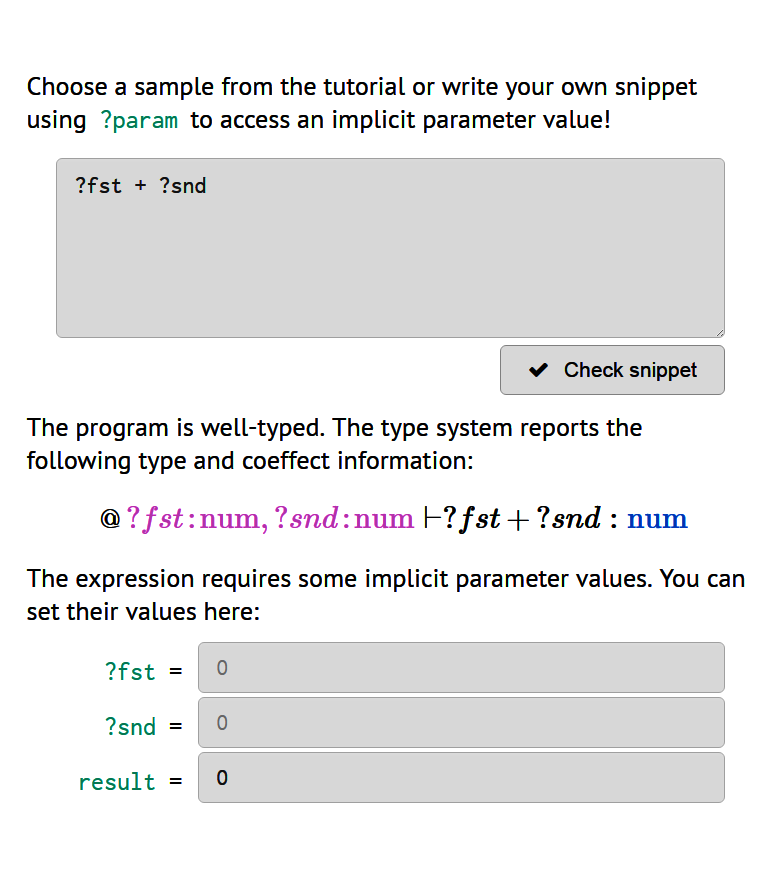
\includegraphics[width=16em]{images/eval1.png}}
\boxed{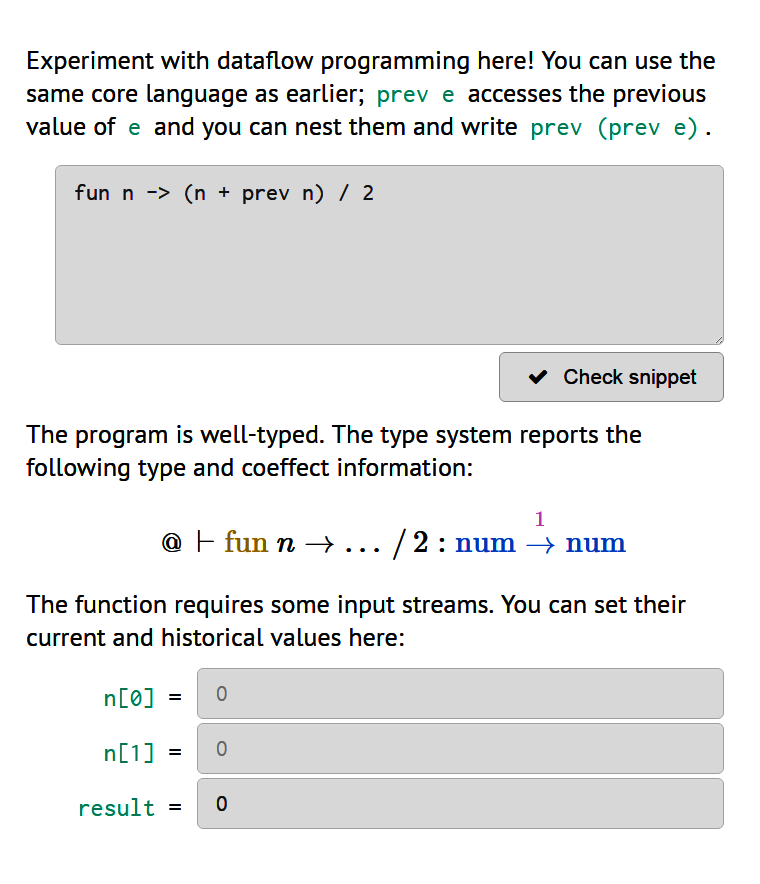
\includegraphics[width=16em]{images/eval2.png}}
\caption{Interactive evaluation of implicit parameters (left) and dataflow (right)}
\label{fig:essay-eval}
\end{figure}

% --------------------------------------------------------------------------------------------------

\section{Interactive essay}
\label{sec:impl-essay}

As explained in the introduction of this chapter, the purpose of the implementation presented in
this thesis is not to provide a real-world programming language, but to support the theory
discussed in the rest of the thesis. The goal is to explain the theory and inspire authors of
real-world programming languages to include support for context-aware programming, ideally using
coeffects as a sound foundation. For this reason, the implementation needs to be:

\begin{itemize}
\item {\sc Accessible.}  Anyone interested should be able to experiment with the implemented languages
  without downloading the source code and compiling it and without installing specialized software.

\item {\sc Explorable.}  It should be possible to explore the inner workings -- how is the typing
  derived, how is the source code translated to the target language and how is it evaluated.
\end{itemize}

\noindent
To make the work \emph{accessible}, we implement sample context-aware languages in a way that makes it
possible to use them in any standard web browser with JavaScript support (Section~\ref{sec:impl-essay-tech})
without requiring any server-side component. Following the idea that ``the medium is the message'' \cite{essay-medium},
we choose a medium that encourages \emph{exploration} and make the implementation available not just
as source code that can be compiled and run locally, but also in the format of
an interactive essay (Section~\ref{sec:impl-essay-features}). The live version of the essay can be
found at: \url{http://tomasp.net/coeffects}.

% --------------------------------------------------------------------------------------------------

\begin{figure}[t]
\boxed{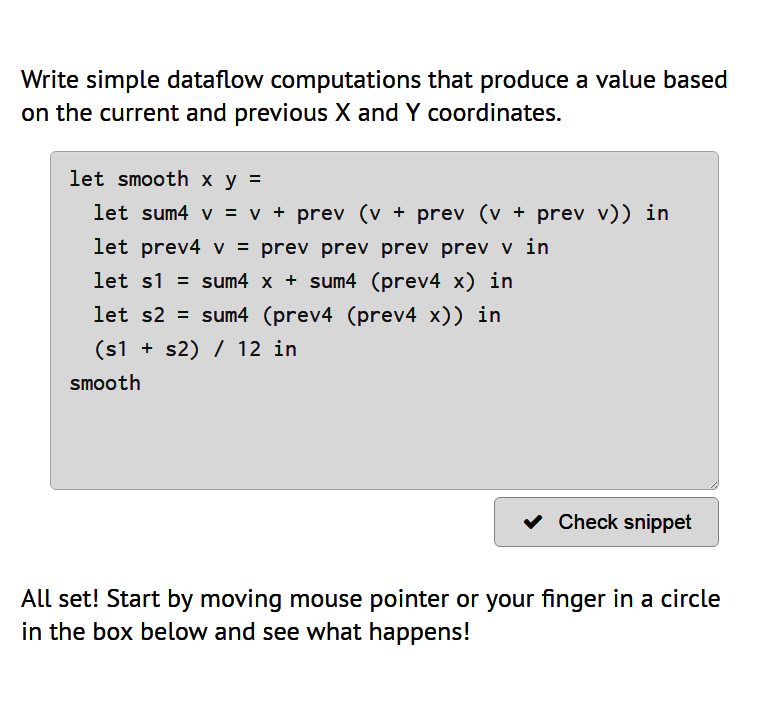
\includegraphics[width=16em]{images/df1.png}}
\boxed{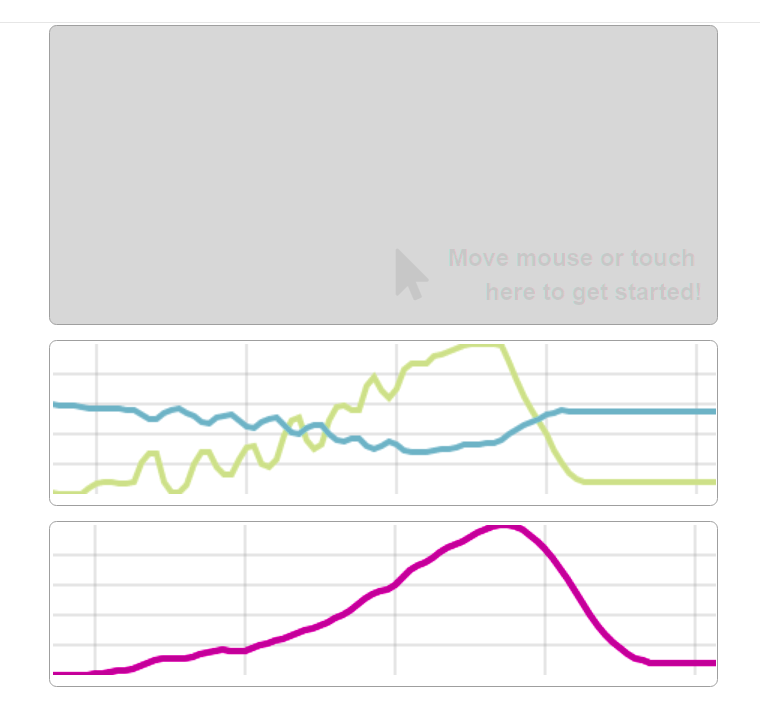
\includegraphics[width=16em]{images/df2.png}}
\caption{Function smoothing the X coordinate (left) with a sample run (right).}
\label{fig:essay-df}
\end{figure}

% --------------------------------------------------------------------------------------------------

\subsection{Explorable language implementation}
\label{sec:impl-essay-features}

The interactive essay format used of the implementation is based on Bret Victor's work on
\emph{explorable explanations} \cite{essay-explorable}. Bret Victor describes what the interactivity
enables as follows:
%
\begin{quote}
\emph{Do our reading environments encourage active reading? Or do they utterly oppose it? A
  typical reading tool, such as a book or website, displays the author's argument, and nothing
  else. The reader's line of thought remains internal and invisible, vague and speculative. We
  form questions, but can't answer them. We consider alternatives, but can't explore them. We
  question assumptions, but can't verify them. And so, in the end, we blindly trust, or blindly
  don't, and we miss the deep understanding that comes from dialogue and exploration.}
\end{quote}
%
The interactive essay we present encourages active reading in the sense summarized in Victor's quote.
We show the reader an example (program, typing derivation or translation), but the reader is
encouraged to modify it and see how the explanation in the essay adapts.

The idea of active reading is older and has been encouraged in the context of art Josef Albers'
classic 1963 work on color \cite{essay-albers} (which was turned into an interactive essay
60 years later \cite{essay-albers-app}). More recently, similar formats have been used to explain
topics in areas such as signal processing \cite{essay-seeing} (explaining Fourier transformations)
and sociology \cite{essay-polygons} (visualizing and explaining game theoretical model of segregation
in the society \cite{essay-segregation}). To our best knowledge, the format has not previously
been used in the area of programming language theory and so we briefly outline some of the
interesting features that our essay provides in order to encourage active reading.

\paragraph{Interactive program execution.}

After providing the practical motivation for coeffects (based on Chapter~\ref{ch:intro}), the
interactive essay shows the reader the two sample context-aware programming languages. Readers can
write code in a panel that type checks the input, generates user interface for entering the
required context and runs the sample code.

The panels for implicit parameters and for dataflow computations are shown in Figure~\ref{fig:essay-eval}.
The sample code on the left adds two implicit parameters and the generated UI lets the user
enter implicit parameter values as required by the context in the typing judgement. The sample on
the right calculates the average of the current and past value in a dataflow; the UI lets the user
enter past values required by the type of the function.

The essay guides the readers through a number of programs (shown in Section~\ref{sec:impl-case-typing})
and encourages them to run and try modifying them. For implicit parameters, this includes the case
where an implicit parameter is available at both declaration site and call site (showing that the
declaration site value is captured). For dataflow, the examples include the comparison between the
inferred type when using flat and structural type systems.

% --------------------------------------------------------------------------------------------------

\begin{figure}[t]
\boxed{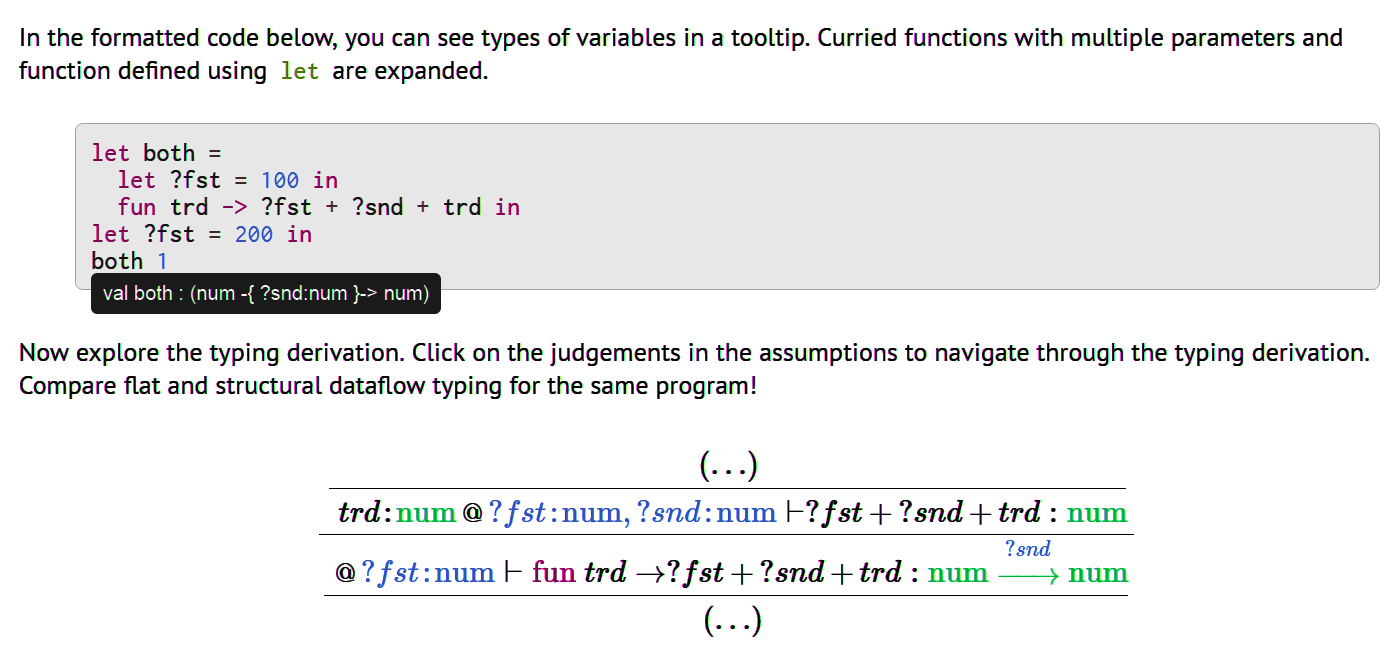
\includegraphics[width=32em]{images/types.png}}
\caption{Source code with type information and explorable typing derivation.}
\label{fig:essay-typing}
\end{figure}

% --------------------------------------------------------------------------------------------------

\paragraph{Reactive dataflow.}

The interactive program execution lets the reader run sample programs, but not in a particularly realistic
context. To show a more real-world scenario, the essay includes a widget shown in Figure~\ref{fig:essay-df}.
This lets the user write a function taking a stream of X and Y coordinates and calculate value
based on the current and past values of the mouse pointer. The X and Y values, together with the
result are plotted using a live chart.

In the example run shown above, the sample program calculates the average of the last 12 values
of the X coordinate (green line in Figure~\ref{fig:essay-df}). The example also illustrates one
practical use of the coeffect type system -- when running, the widget keeps the coordinates in a
pre-allocated fixed-size array, because the coeffect type system guarantees that at most 12 past
values will be accessed.

\paragraph{Explorable typing derivations.}

Perhaps the most important aspect of the implemented context aware programming languages is their
coeffect and type system. In a conventional implementation, the functioning of the type system
would remain mostly hidden -- we would get an ``OK'' message for a well-typed program and a type
error for invalid program (likely not very informative, given that reporting good error messages
for type errors is a notoriously hard problem even for mature language implementations).

The presented interactive essay provides two features to help the reader understand and explore
typing derivations. First, when reading code samples in the text, tooltips show the typing of
individual identifiers, most interestingly functions (Figure~\ref{fig:essay-typing}, above).

Second, a later part of the essay provides a type checker that lets the user enter a source code
in a context aware programming language and produces an explorable typing derivation for the
program. The output (shown in Figure~\ref{fig:essay-typing}, below) displays a typing judgement
with assumptions and conclusions and lets the reader navigate through the typing derivation by
clicking on the assumptions or conclusions. This way, the reader can see how is the final typing
derivation obtained, exploring interesting aspects, such as the abstraction rule (shown in
Figure~\ref{fig:essay-typing}).

\paragraph{Comonadically-inspired translation.}

The last interactive element of the essay lets the reader explore the translation of source
context aware language to a target simple functional language (Section~\ref{sec:impl-theory-transl}).
Compared with the monadic ``do'' notation \cite{other-haskell98}, the comonadic translation is more
complex for two reasons.

First, it merges all variables into a single (comonadic) value representing
the context. Second, there is a flat and structural variation of the system. For these two reasons,
understanding the translation based just on the rules is harder than for monads. The essay lets
readers see translation for carefully chosen case studies that illustrate the key aspects of the
translation (some discussed in Section~\ref{sec:impl-case-transl}), but also for their own
programs encouraging \emph{active reading}. Sample input and output are shown in
Figure~\ref{fig:essay-transl}.

% --------------------------------------------------------------------------------------------------

\begin{figure}[t]
\boxed{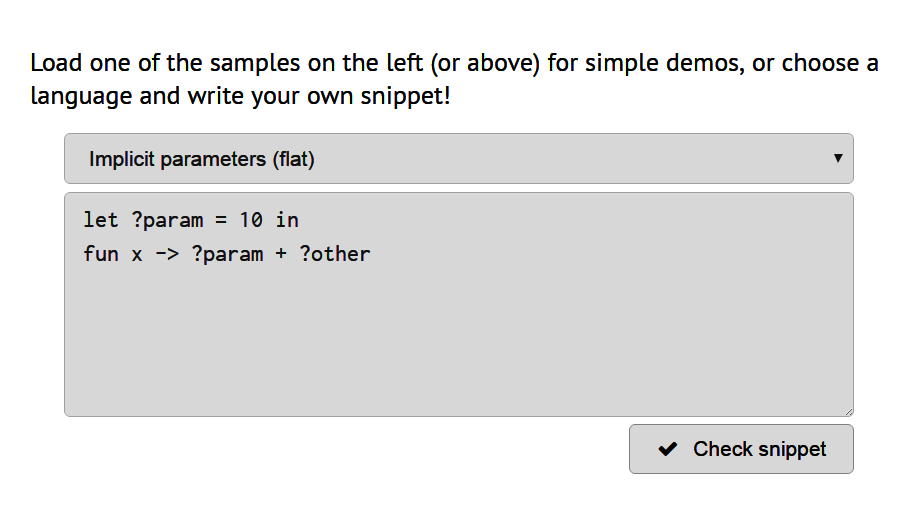
\includegraphics[width=16em]{images/transl1.png}}
\boxed{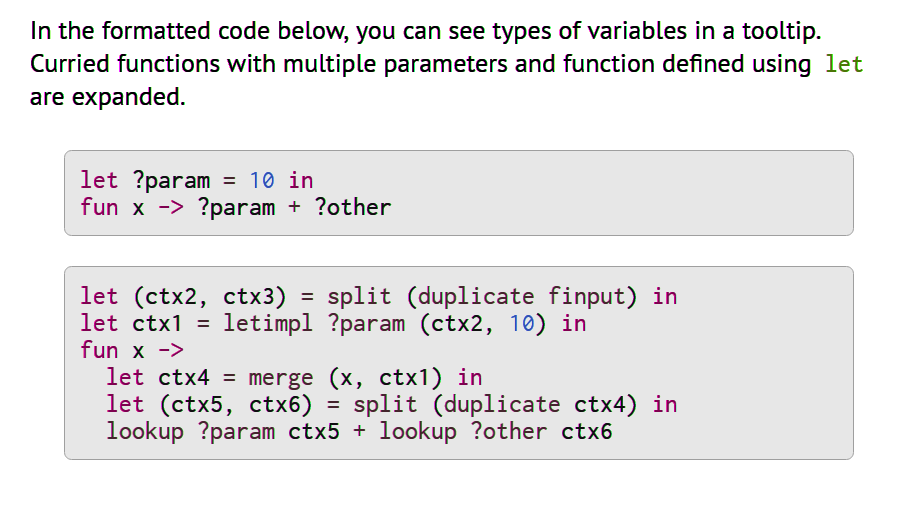
\includegraphics[width=16em]{images/transl2.png}}
\caption{Source code with comonadically-inspired translation}
\label{fig:essay-transl}
\end{figure}

% --------------------------------------------------------------------------------------------------

\subsection{Implementation overview}
\label{sec:impl-essay-tech}

The core part of our implementation mostly follows standard techniques for implementing type
checkers and interpreters for statically-typed functional programming languages. Two interesting
aspects that are worth discussing is the JavaScript targetting (for running the language
implementation in a web browser) and integration with client-side (JavaScript) libraries for
building the user interface. The full source code can be obtained from
\url{https://github.com/coeffects/coeffects-playground}. It is structured as follows:
%
\begin{itemize}
\item Parsing is implemented using a simple parser combinator library; \strf{ast.fs} defines the
  abstract syntax tree for the languages; \strf{parsec.fs} implements the parser combinators
  and \strf{lexer.fs} with \strf{parser.fs} parse the source code by first tokenizing
  the input and then parsing the stream of tokens.

\item The type checking is implemented by \strf{typechecker.fs}, which annotates an untyped AST
  with types and generates set of type and coeffect constraints. The constraints are later solved
  (using domain-specific algorithms for each of the languages) in \strf{solver.fs}.

\item Type-checked programs in context-aware languages are translated to simple target
  functional subset of the language in \strf{translation.fs}; \strf{evaluation.fs} then interprets
  programs in the target language. The interpretation does not handle the source
  language and so programs containing context-aware constructs cannot be interpreted directly.

\item The user interface of the interactive essay (Section~\ref{sec:impl-essay-features})
  is implemented partly in F\# and partly in JavaScript. The two most important components include
  a pretty-printer \strf{pretty.fs} which formats source code (with type tooltips) and typing
  derivations and \strf{gui.fs} that implements user interaction (e.g.~navigation in explorable
  typing derivations).
\end{itemize}

\noindent
As discussed in Section~\ref{sec:impl-theory-ext}, the implementation can be easily extended to
support additional context-aware programming languages. This is due to the fact that it is based
on the unified theory of coeffects. In practice, adding support for liveness tracking would
require adding a domain-specific constraint solver in \strf{solver.fs} and extending the
interpreter in \strf{evaluation.fs} with a new kind of comonadically-inspired data type
(indexed maybe comonad) with its associated operations.

\section{Related work}
\label{sec:impl-related}

To our best knowledge, combining Bret Victor's idea of explorable explanations with programming
language theory (as discussed in Section~\ref{sec:impl-essay}) is a novel contribution of our work.
On the technical side, we build on a number of standard methods.

\paragraph{Parsing and type checking.} The implementation of the parser, type checker and
interpreter follows standard techniques for implementing functional programming languages.
In order to be able to compile the implementation to JavaScript (see below), we built a
small parser combinator library \cite{monad-parsing} rather than using one of the already
available libraries \cite{other-fparsec}.

\paragraph{Targetting JavaScript.} In order to make the implementation accessible to a broad
audience, it can be executed in a web browser. This is achieved by automatically translating the
implementation from F\# to JavaScript. We use an F\# library called FunScript \cite{other-funscript}
(which is a more recent incarnation of the idea developed by the author \cite{app-fsharp-webtools}).
We choose F\#, but similar tools exist for other functional languages such as OCaml \cite{other-js-ocaml}.
It is worth noting that FunScript is implemented as a \emph{library} rather than as a compiler
extension. This is done using the meta-programming capabilities of F\# \cite{app-fsharp-metaprog}.

\paragraph{Client-side library integration.} An interesting aspect of the interactive essay
user interface is the integration with third-party JavaScript libraries. We use a number of
libraries including JQuery (for web browser DOM manipulation) and MathJax \cite{essay-mathjax}
(for rendering of typing derivation). In order to call those from F\# code, we use a number
of mapping methods described in \cite{app-age-of-web}. For example, the following F\# declaration
is used to invoke the \ident{Queue} function in MathJax:
%
\begin{equation*}
\begin{array}{l}
\lbrack\langle\ident{JSEmitInline}(\str{MathJax.Hub.Queue(\{0\});})\rangle\rbrack\\[-0.25em]
\kvd{let}~\ident{queueAction}~(\ident{f}:\ident{unit}~\rightarrow~\ident{unit}):\ident{unit}~=~\ident{failwith}~\str{JS only!}
\end{array}
\end{equation*}
%
The \ident{JSEmitInline} syntax on the first line is an attribute that instructs FunScript
to compile all invocations of the \ident{queueAction} function into the JavaScript literal
specified in the attribute (with \strf{\{0\}} replaced by the argument).


% ==================================================================================================
%
%     #####
%    #     # #    # #    # #    #   ##   #####  #   #
%    #       #    # ##  ## ##  ##  #  #  #    #  # #
%     #####  #    # # ## # # ## # #    # #    #   #
%          # #    # #    # #    # ###### #####    #
%    #     # #    # #    # #    # #    # #   #    #
%     #####   ####  #    # #    # #    # #    #   #
%
% ==================================================================================================

~

\section{Summary}

This chapter supplements the theory of coeffects presented in the previous three chapters with
a prototype implementation. We implemented three simple context-aware programming languages that
track implicit parameters and past values in dataflow computations, the latter both in flat
(per-context) and structural (per-variable) way.

The implementation discussed in this chapter provides an evidence for our claim that the
theory of coeffects can be used as a basis for a wide range of sound context-aware programming
languages. Our implementation consists of a shared coeffect framework (handling type checking and
translation). Each context-aware language then adds a domain-specific rule for choosing a unique
typing derivation, an interpretation of comonadically-inspired primitives and (optionally)
domain-specific primitives such as the \kvd{prev} construct for dataflow.

We make the implementation available in the usual form (as source code that can be downloaded,
compiled and executed), but we also present it in the form of interactive essay. This encourages
\emph{active reading} and lets the reader explore a number of aspects of the implementation
including the type checking (through explorable typing derivations) and the translation. The key
contribution of this thesis is that it provides a unified way for \emph{thinking} about context in
programming languages and the interactive presentation of the implementation is aligned with this
goal. Programming languages of the future will need a mechanism akin to coeffects and we aim to
provide a convincing argument supported by a prototype implementation.

% ==================================================================================================

\chapter{Implementation}
\label{ch:impl}

In the previous three chapters, we presented the theory of coeffects consisting of type system
and comonadically inspired semantics of two parameterized coeffect calculi. The theory provides
a framework that simplifies the implementation of safe context-aware programming languages. To
support this claim, this chapter presents a prototype implementation of three coeffect languages --
language with implicit parameters and both flat and structural versions of a data-flow language.

The implementation directly follows the thoery presented in the previous three chapters. It
consists of a common framework that provides type checking and translation to a simple functional
target language with comonadically-inspired primitives. Each concrete context-aware language then
adds a domain-specific rule for choosing unique typing derivation (as discussed in
Section~\ref{sec:flat-unique}) together with a domain-specific definition of the
comonadically-inspired primitives that define the runtime semantics (see Section~\ref{sec:semantics-proofs}).

The main goal of the implementation is to show that the theory is practically useful and to present it
in a more practical way. However, we do not intend to build a complete real-world programming language.
For this reason, the implementation is available primarilly as an interactive web-based essay, though
it can be also downloaded and run locally.

\paragraph{Chapter structure and contributions}

\begin{itemize}
\item We discuss how the implementation follows from the theory presented earlier (Section~\ref{sec:impl-theory}).
  This applies to the implementation of the \emph{type checker} and the implementation of the \emph{translation}
  to a simple target langauge that is then iterpereted. We also discuss how the common framework makes it
  easy to implement additional context-aware languages (Section~\ref{sec:impl-theory-ext}).

\item We consider a number of case studies (Section~\ref{sec:impl-case}) that illustrate interesting
  aspects of the theories discussed earlier. This includes the typing of lambda abstraction and the
  difference between flat and structural systems (Section~\ref{sec:impl-case-typing}) and the
  comonadically-inspired translation (Section~\ref{sec:impl-case-transl}).

\item The implementation is available not just as downloadable code, but also in the format of
  interactive web-based essay (Section~\ref{sec:impl-essay}), which aims to make coeffects
  accessible to a broader audience. We discuss the most interesting aspects of the essay format and
  briefly discuss some of the interesting implementation detail (Section~\ref{sec:impl-essay-tech}).
\end{itemize}


% ==================================================================================================
%
%    #######
%       #    #    # ######  ####  #####  #   #
%       #    #    # #      #    # #    #  # #
%       #    ###### #####  #    # #    #   #
%       #    #    # #      #    # #####    #
%       #    #    # #      #    # #   #    #
%       #    #    # ######  ####  #    #   #
%
% ==================================================================================================

\section{From theory to implementation}
\label{sec:impl-theory}

The theory discussed so far provides the two key components of the implementation. In
Chapter~\ref{ch:flat}, we discussed the type checking of context-aware programs and
Chapter~\ref{ch:semantics} models the execution of context-aware programs (in terms of
translation and operational semantics). For structural coeffects, the same components are discussed
in Chapter~\ref{ch:structural}. In this section, we discuss how those provide foundation for the
implementation.

% --------------------------------------------------------------------------------------------------

\subsection{Type checking and inference}
\label{sec:impl-theory-typing}

To simplify the writing of context-aware programs, the implementation provides a limited form of
type inference (Section~\ref{sec:impl-tech}). This is available just for convenience and so we do
not claim any completeness or complexity result about the algorithm and we do not present full
formalization. However, it is worth noting how the domain-specific procedures for choosing a unique
type derivation (Section~\ref{sec:flat-unique}) are adapted.

The type inference works in the standard way \cite{types-mlessence,types-inference} by generating
type constraints and solving them. Solving of type constraints is done in the standard way, but we
additionally collect and solve \emph{coeffect constraints}. In order to obtain unique type
derivation, we generate additional coeffect constraints in lambda abstraction of each flat
coeffect language.

\paragraph{Flat implicit parameters.}

As discussed in Section~\ref{sec:flat-unique}, when choosing unique typing derivation for
implicit parameters, we keep track of the implicit parameters available in lexical scope
(written as $\cclrd{\Delta}$). In lambda abstraction rule, the implicit parameters required by
the body (tracked by $\ccclrd{r}$) are split so that all parameters available in lexical scope
are captured and only the remaining parameters ($\cclrd{r}\setminus\cclrd{\Delta}$) are required
from the caller of the function.

From the presentation in Section~\ref{sec:flat-unique}, it might appear that resolving the ambiguity
related to lambda abstraction for implicit parameters requires a type system different from
the core flat coeffect type system shown earlier in Section ~\ref{sec:flat-calculus-types}.
This is not the case.

We track implicit parameters in scope $\cclrd{\Delta}$, but the rest of the (\emph{abs}) rule from
the implementation only generates an additional coeffect constraint. Writing
$\coctx{\Gamma}{\cclrd{t}} \vdash e : \tau ~|~ C}$ for a judgement that generates coeffect
constraints $C$, the (\emph{abs}) rule used for implicit parameters looks as follows:
%
\begin{equation*}
\tyrule{abs}
  {\coctx{\Gamma, x\!:\!\tau_1;\cclrd{\Delta}}{\cclrd{t}} \vdash e : \tau_2 ~|~ C}
  {\coctx{\Gamma;\cclrd{\Delta}}{\cclrd{r}} \vdash \lambda x\!:\!\tau_1.e : \tau_1 \xrightarrow{\cclrd{s}} \tau_2 ~|~
    C\cup\{\cclrd{t}=\cclrd{r} \,\czip\, \cclrd{s}, \cclrd{r}=\cclrd{\Delta} \}}
\end{equation*}
%
Given a typing derivation for the body that produced constraints $C$, we generate an additional
constraint that restricts $\cclrd{r}$ (declaration-site demands) to those available in the
current static scope $\cclrd{\Delta}$. It is not necessary to generate a constraint for the
coeffect $\cclrd{s}$, because our constraint satisfaction algorithm finds
the minimal set $\cclrd{s}$ which is $\cclrd{t}\cclrd{\setminus \Delta}$.

\paragraph{Flat data-flow.}
In context-aware language for data-flow (and in language with liveness tracking), the inherent
ambiguity of the (\emph{abs}) rule is resolved by duplicating the context requirements of the body.
In Section~\ref{sec:flat-unique}, this was defined by replacing the standard coeffect (\emph{abs})
rule with a rule (\emph{idabs}) that uses an annotation $\cclrd{r}$ for the body of the function,
declaration-site coeffect and call-site coeffect.

As with implicit parameters, the implementation does not require changing the core (\emph{abs})
typing rule of the flat coeffect system. Instead, the unique resulution is obtained by generating
additional coeffect constraints:
%
\begin{equation*}
\tyrule{abs}
  {\coctx{\Gamma, x\!:\!\tau_1}{\cclrd{t}} \vdash e : \tau_2 ~|~ C}
  {\coctx{\Gamma}{\cclrd{s}} \vdash \lambda x\!:\!\tau_1.e : \tau_1 \xrightarrow{\cclrd{t}} \tau_2 ~|~
    C\cup\{\cclrd{t}=\cclrd{r} \,\czip\, \cclrd{s}, \cclrd{r}=\cclrd{t}, \cclrd{s}=\cclrd{t} \}}
\end{equation*}
%
Here, the two additional constraints restrict both $\cclrd{r}$ and $\cclrd{s}$ to be equal to the
coeffect of the body $\cclrd{t}$ and so the only possible resolution is the one specified by
(\emph{idabs}).

% --------------------------------------------------------------------------------------------------

\subsection{Execution of context-aware programs}
\label{sec:impl-theory-transl}

Context-aware programs are executed by translating the source program into a simple functional
target language. For simplicity, programs in the simple target language are then interpreted, but
they could equally be compiled using standard techniques for compiling functional code. The
translation follows the rules defined in Section~\ref{sec:semantics-translation} (for flat coeffect
languages) and Section~X (for structural coeffect languages). The result of the translation is a
program that consists of the following:

\begin{itemize}
\item {\sc Functional constructs.} Those include binary operations, tuples, let binding,
  constants, variables, function abstraction and application. The interpreter keeps a map of
  assignments for variables in scope and recursively evaluates the expression.

\item {\sc Comonadic operations.} Those are the comonadic primitives provided by indexed comonads --
  \ident{cobind}, \ident{counit} together with \ident{merge} and \ident{split} for flat coeffects
  or \ident{merge} and \ident{choose} for structural coeffects. The translation that produces these
  is shared by all context-aware languages, but their definition in the interpreter is
  domain-specific.

\item {\sc Domain-specific operations.} Each context-aware language may additionally include
  operations that model domain-specific operations. For data-flow, this is \ident{prev} (accessing
  past values) and for implicit parameters, this is \ident{letimpl} and \ident{lookup} for implicit
  parameter binding and access, respectively.
\end{itemize}

\noindent
The fact that the prototype implementation is based on the theoretical framework provided by
coeffect calculi means that it has the desirable properties proved in Section~\ref{sec:semantics-proofs}
and Section~X. In particular, evaluating a well-typed context-aware program in a context that
provides sufficient contextual capabilities will not cause an error.

In the interactive essay (Section~\ref{sec:impl-essay}), we further use the coeffects to
automatically generate a user interface that requires the user to provide the required contextual
capabilities (past values for individual variables, or values for implicit parameters).

Another benefit of using the common framework is that the implementation can be easily extended
to support additional context-aware languages.

% --------------------------------------------------------------------------------------------------

\subsection{Supporting additional context-aware languages}
\label{sec:impl-theory-ext}

The prototype implementation supports two of the context-aware languages discussed in this thesis:
implicit parameters and data-flow. The remaining examples are calculus for tracking variable
liveness (of ordinary variables) and the structural language based on bounded reuse (counting
number of times values are used). However, the prototype implementation is based on the
common coeffect framework and makes it easy to add support for these and also for other context
aware languages based on coeffects.

In order to extend the implementation with support for liveness or bounded reuse tracking (or
other context-aware language), the following 4 additions are required:

\begin{enumerate}
\item A domain-specific function abstraction rule that resolves the ambiguity in the general
  (\emph{abs}) rule of the flat coeffect calculus. For liveness, the handling would be the same
  as for data-flow, but for other flat coeffect systems, another resolution mechanism might be used
  instead.

\item A domain-specific instance of coeffect algebra needs to be provided. In order to support
  the type inference in the prototype implementation, the constraint solver needs to be extended
  to solve constraint using the coeffect algebra. For liveness, this would be solving simple
  two-point lattice constraints.

\item For evaluation, a new kind of comonadic values needs to be added. For liveness, this would be
  an option value that may or may not contain a value. The semantics of comonadic operations on the
  values needs to be defined.

\item For context-aware languages that have additional primitives (such as \kvd{prev} or \ident{?param}),
  the parser and AST needs to be extended, custom type-checking and translation rules added and
  domain-specific primitive operations (with their semantics) provided. Liveness and bounded reuse
  do not have additional custom syntax and so supporting these would not require this step.
\end{enumerate}

\noindent
The list mirrors a list of steps that need to be done when supporting a new effectful computation
in a language that supports monadic do-notation. The step (3) corresponds to implementing a new
monad and (4) corresponds to adding monad-specific effectful operations. The step (2) applies when
using indexing to track effects more precisely \cite{effects-embedding}. The only step that does not
have effectful/monadic counterpart is (1).

When adding a new context-aware programming language support, much of the existing infrastructure
can be reused. This includes the implementation of the core coeffect and type checking rules and
also the translation for standard language constructs as well as the interpreter for the target
language.


% ==================================================================================================
%
%     #####
%    #     #   ##    ####  ######     ####  ##### #    # #####  # ######  ####
%    #        #  #  #      #         #        #   #    # #    # # #      #
%    #       #    #  ####  #####      ####    #   #    # #    # # #####   ####
%    #       ######      # #              #   #   #    # #    # # #           #
%    #     # #    # #    # #         #    #   #   #    # #    # # #      #    #
%     #####  #    #  ####  ######     ####    #    ####  #####  # ######  ####
%
% ==================================================================================================

\section{Case studies}
\label{sec:impl-case}

The prototype implementation illustrates a number of interesting aspects of coeffect systems.
Those appear as examples in the interactive essay (discussed in Section~\ref{sec:impl-essay}), but
we briefly review them in this section.

% --------------------------------------------------------------------------------------------------

\subsection{Typing context-aware programs}
\label{sec:impl-case-typing}

We first consider two case studies of how coeffect type checking works. The first one exposes the
resolution of the ambiguity in typing for implicit parameters and the second one exposes the
difference between flat and structural system for data-flow.

\paragraph{Abstraction for implicit parameters.}
As discussed in Section~\ref{sec:impl-theory-typing}, the implementation of the language with
implicit parameters resolves the ambiguity in the lambda abstraction by generating a coeffect
constraint that restricts the set of parameters required from the declaration-site to those that
are lexically available. Remaining parameters are required from the call-site. This is illustrated
by the following example:
%
\begin{equation*}
\begin{array}{l}
\kvd{let}~\ident{both}~=\\[-0.25em]
\quad \kvd{let}~\ident{?fst}~=~100~\kvd{in}\\[-0.25em]
\quad \kvd{fun}~\ident{trd}~\rightarrow~\ident{?fst}~+~\ident{?snd}~+~\ident{trd}~\kvd{in}\\[-0.25em]
\kvd{let}~\ident{?fst}~=~200~\kvd{in}\\[-0.25em]
\ident{both}~1
\end{array}
\end{equation*}
%
In this expression, the lambda function on line 3 requires implicit parameters \ident{?fst} and
\ident{?snd}. Since \ident{?fst} is available in scope, the type of \ident{both} is a function that
requires only \ident{?snd}. In the text-based notation used in the prototype, the type of the
function \ident{both} is: {\tt num -\{?snd:num\}-> num}.

\paragraph{Flat and structural data-flow.}
In flat data-flow, the context requirements of the body is required from both the declaration-site
and from the call-site. In structural data-flow, the context requirements are tracked separately
for each variable, which provides a more precise type. Consider the following two examples (the
\kvd{let} keyword is used to define a curried function of two arguments):
%
\begin{equation*}
\begin{array}{l}
\kvd{let}~\ident{oldy}~\ident{x}~\ident{y}~=~\ident{x}~+~\kvd{prev}~\ident{y}~\kvd{in}\\[-0.25em]
\ident{oldy}
\end{array}
\end{equation*}
%
When type checking the expression using the flat system, the type of \ident{oldy} is inferred as {\tt num -\{1\}-> num -\{1\}-> num},
but when using the structural system, the type becomes {\tt num -\{0\}-> num -\{1\}-> num}.

This illustrates the difference between the two - the flat system keeps only one annotation
for the whole body (which requires 1 past value). In lambda abstraction (or function declaration
written using \kvd{let}), this requirement is duplicated. The structural system keeps information
per-variable and so the resulting type reflects the fact that only the variable \idnet{y} appears
inside \kvd{prev}.

% --------------------------------------------------------------------------------------------------

\subsection{Comonadically-inspired translation}
\label{sec:impl-case-transl}

In addition to running coeffect programs, the implementation can also print the result of the
translation to the simple functional target language with comonadically-inspired primitives.
The following two case studies illustrate important aspects of the translation for flat coeffect
systems (Section~\ref{sec:semantics-translation}) and structural coeffect systems (Section~?).

\paragraph{Merging implicit parameter contexts.}

The following example illustrates the lambda abstraction for implicit parameters.
It defines a parameter \ident{?param} and then returns a function value that captures it, but
also requires an implicit parameter \ident{?other}:
%
\begin{equation*}
\begin{array}{l}
\kvd{let}~\ident{?param} ~=~ \num{10}~\kvd{in}\\[-0.25em]
\kvd{fun}~\ident{x}~\rightarrow~\ident{?param} ~+~ \ident{?other}
\end{array}
\end{equation*}
%
Translating the code to the target language produces the code below. The reader is encouraged to
view the translation in the interactive essay (Section~\ref{sec:impl-essay}), which displays the
types and coeffect annotations of the individual values and primitives. As in the theory, the
comonadically-inspired primitives are families of operations indexed by the coeffects (we
omit the annotations here):
%
\begin{equation*}
\begin{array}{l}
\kvd{let}~(\ident{ctx2}, \ident{ctx3}) ~=~ \ident{split}~(\ident{duplicate}~\kvd{finput})~\kvd{in}\\[-0.25em]
\kvd{let}~\ident{ctx1} ~=~ \ident{letimpl}_{\ident{?param}}~(\ident{ctx2}, \num{10})~\kvd{in}\\[-0.25em]
\kvd{fun}~\ident{x}~\rightarrow\\[-0.25em]
\quad \kvd{let}~\ident{ctx4} ~=~ \ident{merge}~(\ident{x}, \ident{ctx1})~\kvd{in}\\[-0.25em]
\quad \kvd{let}~(\ident{ctx5}, \ident{ctx6}) ~=~ \ident{split}~(\ident{duplicate}~\ident{ctx4})~\kvd{in}\\[-0.25em]
\quad \ident{lookup}_{\ident{?param}}~\ident{ctx5} ~+~ \ident{lookup}_{\ident{?other}}~\ident{ctx6}
\end{array}
\end{equation*}
%
The \kvd{finput} value on the first line represents an empty context in which the expression is
evaluated and is of type $\ctyp{\czero}{\ident{unit}}$. The context is duplicated; \ident{ctx3}
is not needed, because $\num{10}$ is a constant; \ident{ctx2} is passed to \ident{letimpl}, which
assigns an implicit parameter value in the newly returned context \ident{ctx1} of type
$\ctyp{\cclrd{\{\ident{?param}\}}}{\ident{unit}}$ (this now carries the implicit parameter value, but
it does not represent any ordinary variables, thus the \ident{unit} type representing an empty
tuple).

In the body of the function, the context \ident{ctx1} is merged with the context provided by the
variable \ident{x}. The type of \ident{ctx4} is $\ctyp{\ccrld{\{\ident{?param},\ident{?other}\}}}{(\ident{num}\times\ident{unit})}$.
This is then split into two parts that contain just one of the implicit parameters and those are
then accessed using \ident{lookup}.

\paragraph{Composition in structural data-flow.}

In structural coeffect systems, the translation works differently in that the context passed to
a sub-expression contains only assignments for the variables used in the sub-expression (in the
flat version, we always duplicated the variable context before using \ident{split}). To illustrate
this, consider the following simple function:
%
\begin{equation*}
\begin{array}{l}
\kvd{fun}~\ident{x} \rightarrow \kvd{fun}~\ident{y} \rightarrow \kvd{prev}~\ident{x}
\end{array}
\end{equation*}
%
In structural coeffect systems, the comonadic value is annotated with a vector of coeffect
annotations that correspond to individual variables. The initial structural input \kvd{sinput}
is a value of type $\ctyp{\cclrd{[]}}{()}$ containing no variables (we write $()$ rather than
\ident{unit} to make that more explicit). The translated code then looks as follows:
%
\begin{equation*}
\begin{array}{l}
\kvd{fun}~\ident{x} \rightarrow\\[-0.25em]
\quad \kvd{let}~\ident{ctx1} ~=~ \ident{merge}~(\ident{x}, \kvd{sinput}) \kvd{in}\\[-0.25em]
\quad (\kvd{fun}~\ident{y} \rightarrow\\[-0.25em]
\quad \quad \kvd{let}~\ident{ctx2} ~=~ \ident{merge}~(\ident{y}, \ident{ctx1})~\kvd{in}\\[-0.25em]
\quad \quad \ident{counit}~(\ident{prev}~(\ident{choose}_{\langle 0,1\rangle}~\ident{ctx2}))
\end{array}
\end{equation*}
%
The two variables are merged with the initial context, obtaining a value \ident{ctx2} of type
$\ctyp{\cclrd{[0, 1]}}{\ident{num}\times\ident{num}}$ that contains two values with 0 and 1 past
values, respectively.

For simplicity, the implementation does not use the \ident{split}/\ident{merge} pair of operations
of the structural coeffects to obtain the correct subset of variables. This can be done, but it
would make the translated code longer and more cumbersome. Instead, we use a higher-level operation
\ident{choose} (which can be expressed in terms of \ident{split}/\ident{merge}) that projects the
variable subset as specified by the index. Here, $\langle 0, 1\rangle$ means that the first variable
should be dropped an the second one should be kept.

The resulting single-variable context is then passed to \ident{prev} (to shift the stream by one)
and then to \ident{counit} to obtain the current value.


% ==================================================================================================
%
%    #######
%    #        ####   ####    ##   #   #
%    #       #      #       #  #   # #
%    #####    ####   ####  #    #   #
%    #            #      # ######   #
%    #       #    # #    # #    #   #
%    #######  ####   ####  #    #   #
%
% ==================================================================================================

\section{Interactive essay}
\label{sec:impl-essay}

As explained in the introduction of this chapter, the purpose of the implementation presented in
this thesis is not to provide a real-world programming language, but to support the theory
discussed in the rest of the thesis. The goal is to explain the theory and inspire authors of
real-world programming langauges to include support for context-aware programming, ideally using
coeffects as a sound foundation. For this reason, the implementation needs to be:

\begin{itemize}
\item {\sc Accessible.}  Anyone interested should be able to use the implemented langauges without
  downloading the source code and compiling it and without installing specialized software.

\item {\sc Explorable.}  It should be possible to explore the inner workings -- how is the typing
  derived, how is the source code translated to the target language and how is it evaluated.
\end{itemize}

\noindent
To make the work \emph{accessible}, we implement sample context-aware languages in a way that makes it
possible to use them in any standard web browser with JavaScript support (Section~\ref{sec:impl-essay-tech})
without requiring any server-side component. Following the idea that ``the medium is the message'' \cite{essay-medium},
we choose medium that encourages \emph{exploration} and make the implementation available not just
as source code that can be compiled and run locally, but also in the format of
interactive essay (Section~\ref{sec:impl-essay-features}). The live version of the essay can be
found at: \url{http://tomasp.net/coeffects}.

% --------------------------------------------------------------------------------------------------

\begin{figure}[t]
\boxed{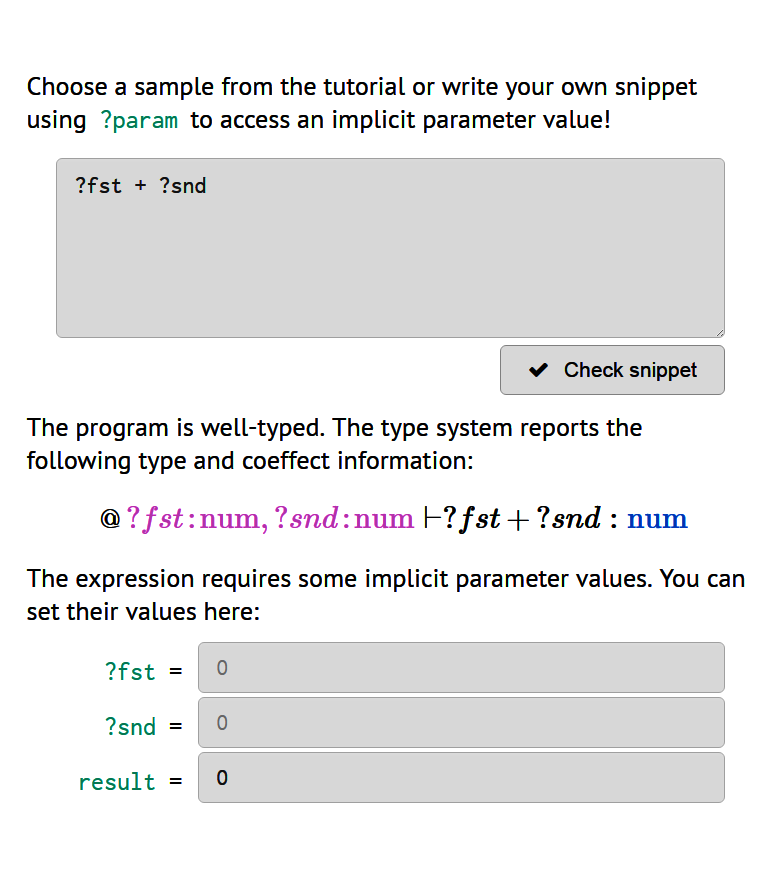
\includegraphics[width=16em]{images/eval1.png}}
\boxed{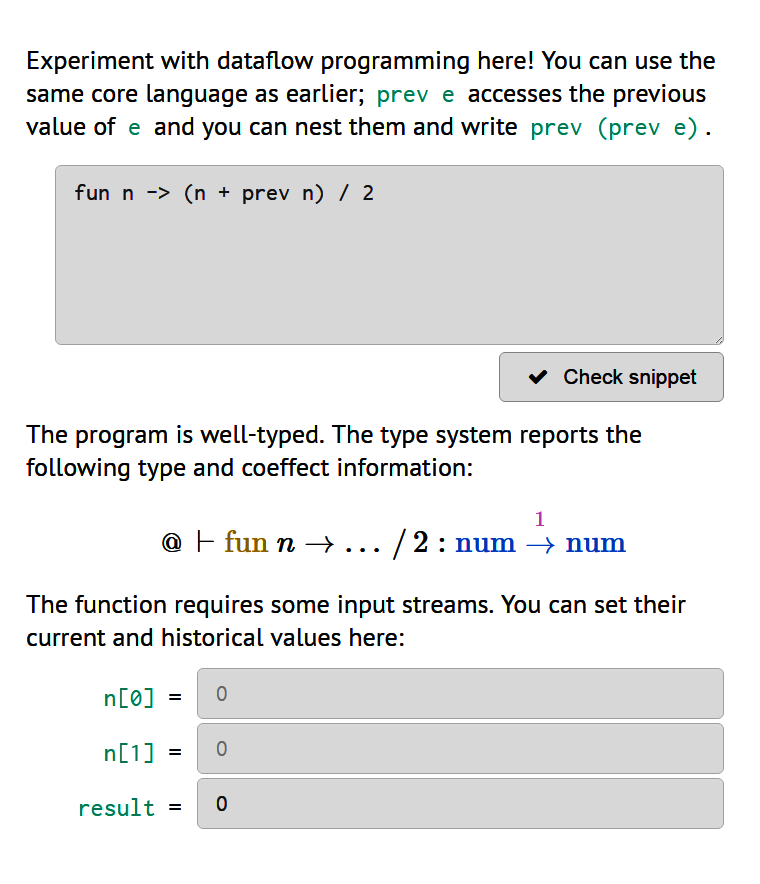
\includegraphics[width=16em]{images/eval2.png}}
\caption{Interactive evaluation of implicit parameters (left) and data-flow (right)}
\label{fig:essay-eval}
\end{figure}

% --------------------------------------------------------------------------------------------------

\subsection{Explorable language implementation}
\label{sec:impl-essay-features}

The interactive essay format used of the implementation is inspired by Bret Victor's work on
\emph{explorable explanations} \cite{essay-explorable}:
%
\begin{quote}
\emph{Do our reading environments encourage active reading? Or do they utterly oppose it? A
  typical reading tool, such as a book or website, displays the author's argument, and nothing
  else. The reader's line of thought remains internal and invisible, vague and speculative. We
  form questions, but can't answer them. We consider alternatives, but can't explore them. We
  question assumptions, but can't verify them. And so, in the end, we blindly trust, or blindly
  don't, and we miss the deep understanding that comes from dialogue and exploration.}
\end{quote}
%
The interactive essay we present encourages active reading in the sense summarized in Victor's quote.
We show the reader an example (program, typing derivation or translation), but the reader is
encouraged to modify it and see how the explanation in the essay adapts.

The idea of active reading is older and has been encouraged in the context of art Josef Albers'
classic 1963 work on color \cite{essay-albers} (which has been turned into an interactive essay
60 years later \cite{essay-albers-app}). More recently, similar formats have been used to explain
topics in areas such as signal processing \cite{essay-seeing} (explaining Fourrier transformations)
and sociology \cite{essay-polygons} (visualizing and explaining game theoretical model of segregation
in the society \cite{essay-segregation}). To our best knowledge, no such work exists in the area
of programming language theory and so we briefly outline some of the interesting features that
our essay provides in order to encourage active reading.

\paragraph{Interactive program excution.}

After providing the practical motivation for coeffects (based on Chapter~\ref{ch:intro}), the
interactive essay shows the reader the two sample context-aware programming languages. Readers can
write code in a panel that type checks the input, generates user interface for entering the
required context and runs the sample code.

The panels for implicit parameters and for data-flow computations are shown in Figure~\ref{fig:essay-eval}.
The sample code on the left adds two implicit parameters and the generated UI lets the user
enter implicit parameter values as required by the context in the typing judgement. The sample on
the right calculates the average of the current and past value in a data-flow; the UI lets the user
enter past values required by the type of the function.

The essay guides the readers through a number of interesting programs (shown in Section~\ref{sec:impl-case-typing})
and encourages them to run and try modifying them. For implicit parameters, this includes the case
where an implicit parameter is available at both declaration-site and call-site (showing that the
declaration-site value is captured). For data-flow, the examples include the comparison between the
inferred type when using flat and structural type systems.

% --------------------------------------------------------------------------------------------------

\begin{figure}[t]
\boxed{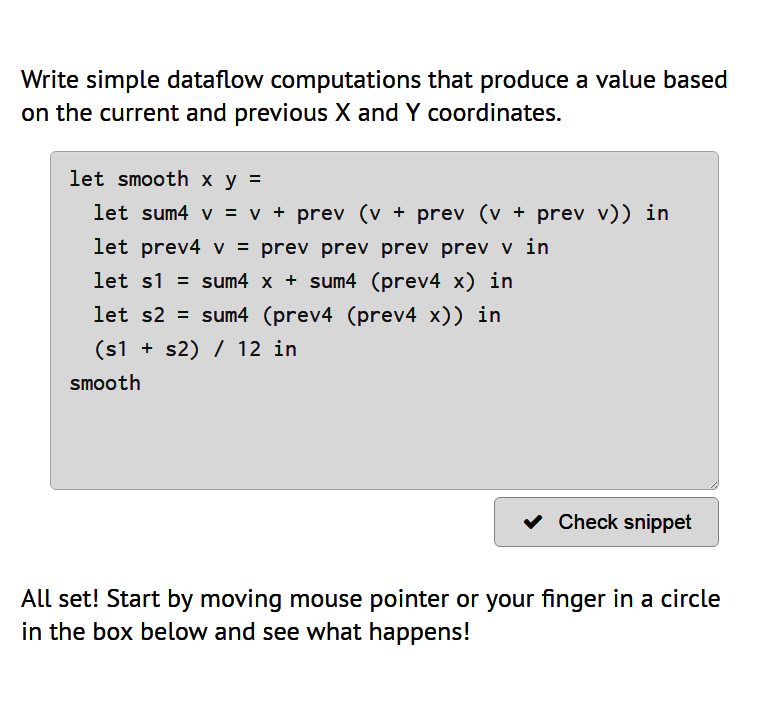
\includegraphics[width=16em]{images/df1.png}}
\boxed{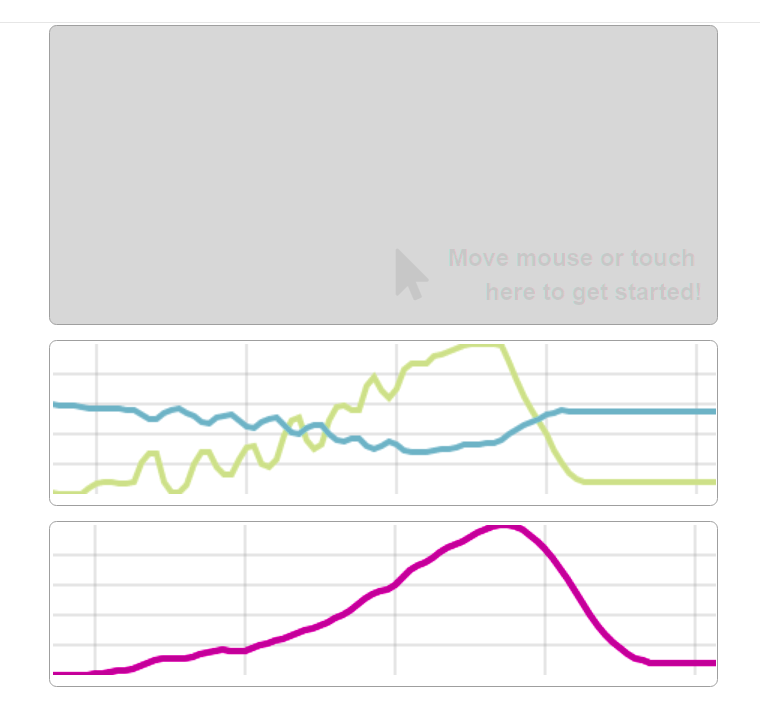
\includegraphics[width=16em]{images/df2.png}}
\caption{Function smoothing the X coordinate (left) with a sample run (right).}
\label{fig:essay-df}
\end{figure}

% --------------------------------------------------------------------------------------------------

\paragraph{Reactive data-flow.}

The interactive program execution lets the reader run sample programs, but not in a realistic
context. To show a more real-world scenario, the essay includes a widget shown in Figure~\ref{fig:essay-df}.
This lets the user write a function taking a stream of X and Y coordinates and calculate value
based on the current and past values of the mouse pointer. The X and Y values, together with the
result are plotted using a live chart.

In the example run shown above, the sample program calculates the average of the last 12 values
of the X coordinate (green line in Figure~\ref{fig:essay-df}). The example also illustrates one
practical use of the coeffect type system -- when running, the widget keeps the coordinates in a
pre-allocated fixed-size array, because the coeffect type system guarantees that at most 12 past
values will be accessed.

% --------------------------------------------------------------------------------------------------

\begin{figure}[t]
\boxed{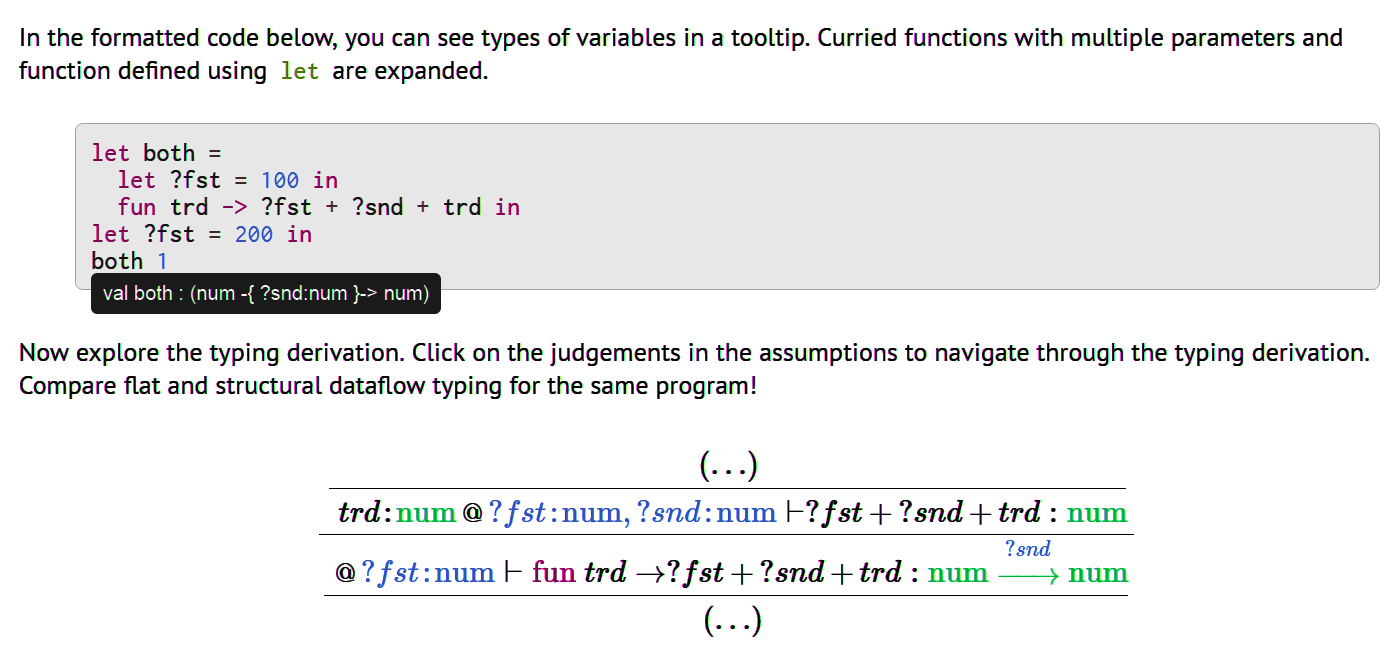
\includegraphics[width=32em]{images/types.png}}
\caption{Source code with type information and explorable typing derivation.}
\label{fig:essay-typing}
\end{figure}

% --------------------------------------------------------------------------------------------------

\paragraph{Explorable typing derivations.}

Perhaps the most important aspect of the implemented context aware programming languages is their
coeffect and type system. In a conventional implementation, the functioning of the type system
would remain mostly hidden -- we would get an ``OK'' message for a well-typed program and a type
error for invalid program (likely not very informative, given that reporting good error messages
for type errors is a notoriously hard problem even for mature language implementations).

The presented interactive essay provides two features to help the reader understand and explore
typing derivations. First, when reading code samples in the text, tooltips show the typing of
individual identifiers, most interestingly functions (Figure~\ref{fig:essay-typing}, above).

Second, a later part of the essay provides a type checker that lets the user enter a source code
in a context aware programming language and produces an explorable typing derivation for the
program. The output (shown in Figure~\ref{fig:essay-typing}, below) displays a typing judgement
with assumptions and conclusions and lets the reader navigate through the typing derivation by
clicking on the assumptions or conclusions. This way, the reader can see how is the final typing
derivation obtained, exploring interesting aspects, such as the abstraction rule (shown in
Figure~\ref{fig:essay-typing}).

\paragraph{Comonadically-inspired translation.}

The last interactive element of the essay lets the reader explore the translation of source
context aware language to a target simple functional language (Section~\ref{sec:impl-theory-transl}).
Compared with the monadic do-notation \cite{other-haskell98}, the comonadic translation is more
complex for two reasons. First, it merges all variables into a single (comonadic) value representing
the context. Second, there is a flat and structural variation of the system. For these two reasons,
understanding the translation based just on the rules is harder than for monads. The essay lets
readers see translation for carefuly chosen case studies that illustrate the key aspects of the
translation (some discussed in Section~\ref{sec:impl-case-transl}), but also for their own
programs encouraging \emph{active reading}. Sample input and output are shown in
Figure~\ref{fig:essay-transl}.


% --------------------------------------------------------------------------------------------------

\begin{figure}[t]
\boxed{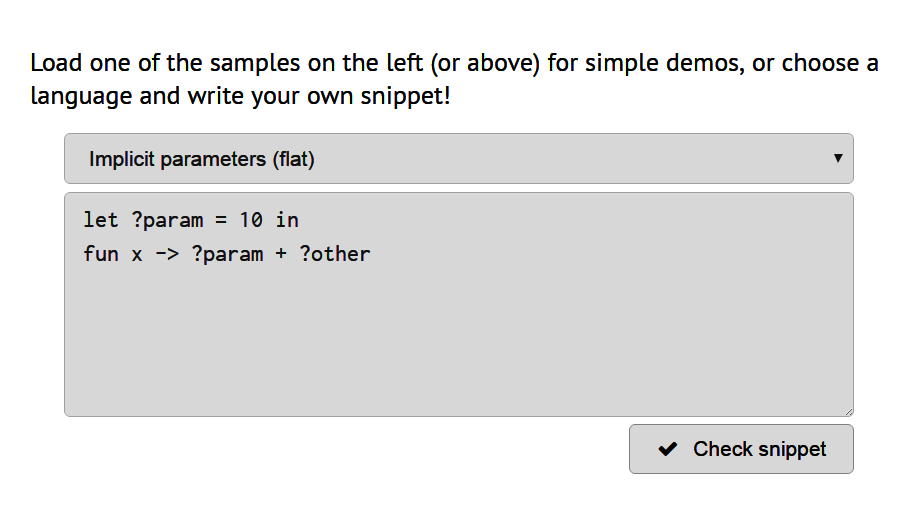
\includegraphics[width=16em]{images/transl1.png}}
\boxed{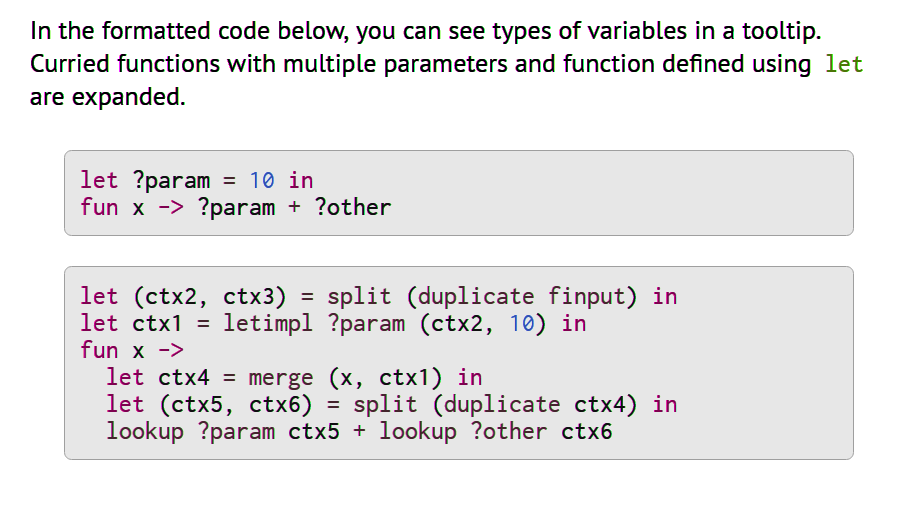
\includegraphics[width=16em]{images/transl2.png}}
\caption{TBD}
\label{fig:essay-transl}
\end{figure}

% --------------------------------------------------------------------------------------------------

\subsection{Implementation overview}
\label{sec:impl-essay-tech}

The core part of our implementation mostly follows standard techniques for implementing type
checkers and interpreters for statically-typed functional programming langauges. Two interesting
aspects that are worth discussing is the JavaScript targetting (for running the langauge
implementation in a web browser) and integration with client-side (JavaScript) libraries for
building the user interface. The full source code can be obtained from
\url{https://github.com/coeffects/coeffects-playground} and is structured as follows:
%
\begin{itemize}
\item Parsing is implemented using smple parser combinator library; \strf{ast.fs} defines the
  abstract syntax tree for the languages; \strf{parsec.fs} implements a small parser combinator
  library and \strf{lexer.fs} with \strf{parser.fs} parse the source code by first tokenizing
  the input and then parsing the stream of tokens.

\item The type checking is implemented by \strf{typechecker.fs}, which annotates an untyped AST
  with types and generates set of type and coeffect constraints. The constraints are later solved
  (using domain-specific algorithms for each of the languages) in \strf{solver.fs}.

\item Type-checked programs in context-aware languages are translated to simple target
  functional subset of the language in \strf{translation.fs}; \strf{evaluation.fs} then interprets
  programs in the target language. The interpretation does not handle the source
  language and so programs containing context-aware contstructs cannot be interpreted directly.

\item The user interface of the interactive essay discussed in Section~\ref{sec:impl-essay-features}
  is implemented partly in F\# and partly in JavaScript. The two most important components include
  a pretty-printer \strf{pretty.fs} which formats source code (with type tooltips) and typing
  derivations and \strf{gui.fs} that implements user interaction (e.g.~navigation in explorable
  typing derivations).
\end{itemize}

\noindent
As discussed in Section~\ref{sec:impl-theory-ext}, the implementation can be easily extended to
support additional context-aware programming languages. This is due to the fact that it is based
on the unified theory of coeffects. In practice, adding support for liveness tracking would
require adding a domain-specific constraint solver in \strf{solver.fs} and extending the
interpreter in \strf{evaluation.fs} with a new kind of comonadically-inspired data type
(indexed maybe comonad) with its associated operations.

\section{Related work}
\label{sec:impl-related}

To our best knowledge, combining Bret Victor's idea of explorable explanations with programming
language theory (as discussed in Section~\ref{sec:impl-essay}) is a novel contribution of our work.
On the technical side, we build on a number of standard methods.

\paragraph{Parsing and type checking.} The implementation of the parser, type checker and
interpreter follows standard techniques for implementing functional programming languages.
In order to be able to compile the implementation to JavaScript (see below), we built a
small parser combinator library \cite{monad-parsing} rather than using one of the already
available libraries \cite{other-fparsec}.

\paragraph{Targetting JavaScript.} In order to make the implementation accessible to a broad
audience, it can be executed in a web browser. This is achieved by automatically translating the
implementation from F\# to JavaScript. We use an F\# library called FunScript \cite{other-funscript}
(which is a more recent incarnation of the idea developed by the author \cite{app-fsharp-webtools}).
We choose F\#, but similar tools exist for other functional languages such as OCaml \cite{other-js-ocaml}.
It is worth noting that FunScript is implemented as a \emph{library} rather than as a compiler
extension. This is done using the meta-programming capabilities of F\# \cite{app-fsharp-metaprog}.

\paragraph{Client-side library integration.} An interesting aspect of the interactive essay
user interface is the integration with third-party JavaScript libraries. We use a number of
libraries including JQuery (for web browser DOM manipulation) and MathJax \cite{essay-mathjax}
(for rendering of typing derivation). In order to call those from F\# code, we use a number
of mapping methods described in \cite{app-age-of-web}. For example, the following F\# declaration
is used to invoke the \ident{Queue} function in MathJax:
%
\begin{equation*}
\begin{array}{l}
\lbrack\langle\ident{JSEmitInline}(\str{MathJax.Hub.Queue(\{0\});})\rangle\rbrack\\[-0.25em]
\kvd{let}~\ident{queueAction}~(\ident{f}:\ident{unit}~\rightarrow~\ident{unit}):\ident{unit}~=~\ident{failwith}~\str{JS only!}
\end{array}
\end{equation*}
%
The \ident{JSEmitInline} syntax on the first line is an attribute that instructs FunScript
to compile all invocations of the \ident{queueAction} function into the JavaScript literal
specified in the attribute (with \strf{\{0\}} replaced by the argument).


% ==================================================================================================
%
%     #####
%    #     # #    # #    # #    #   ##   #####  #   #
%    #       #    # ##  ## ##  ##  #  #  #    #  # #
%     #####  #    # # ## # # ## # #    # #    #   #
%          # #    # #    # #    # ###### #####    #
%    #     # #    # #    # #    # #    # #   #    #
%     #####   ####  #    # #    # #    # #    #   #
%
% ==================================================================================================

\section{Summary}

This chapter supplements the theory of coeffects presented in the previous three chapters with
a prototype implementation. We implemented three simple context-aware programming langauges that
track implicit parameters and past values in dataflow computations (in flat and structural way).

The implementation discussed in this chapter provides an evidence for our claim that the
theory of coeffects can be used as a basis for a wide range of sound context-aware programming
languages. Our implementation consists of a shared coeffect framework (handling type checking and
translation). Each context-aware language then adds a domain-specific rule for choosing a unique
typing derivation, an interpretation of comonadically-inspired primitives and (optionally)
domain-specific primitives such as the \kvd{prev} construct for dataflow.

We make the implementation available in the usual form (as source code that can be downloaded,
compiled and executed), but we also present it in the form of interactive essay. This encourages
\emph{active reading} and lets the reader explore a number of aspects of the implementation
including the type checking (through explorable typing derivations) and the translation. The key
contribution of this thesis is that it provides a unified way for \emph{thinking} about context in
programming langauges and the interactive presentation of the implementation is aligned with this
goal. Programming languages of the future will need a mechanism akin to coeffects and we aim to
provide a convincing argument supported by a prototype implementation.

\chapter{Conclusions and further work} 
\label{ch:conclusions}

Some of the most fundamental academic work is not the one solving hard research problems, but the
one that changes how we understand the world. Some philosophers argue that \emph{language} is the
key for understanding how we think, while in science the dominant thinking is determined by
\emph{paradigms} \cite{philosophy-kuhn} or \emph{research programmes} \cite{philosophy-lakatos}.
In a way, programming languages play a similar role for computer science and software development.

This thesis aims to change how developers and programming language designers think about
\emph{context} or \emph{execution environments} of programs. Such context or execution environment
has numerous forms -- mobile applications access network, GPS location or user's personal data;
journalists obtain information published on the web or through open government data initiatives;
in data-flow programming, we have access to past values of expressions.
This thesis aims to change our understanding of \emph{context} so that the above examples are
viewed uniformly through a single programming language abstraction, which we call \emph{coeffects},
rather than as disjoint cases.

In this chapter, we give a brief summary of the technical development completed in this thesis
(Section~\ref{sec:conc-summary}). The thesis looks at two kinds of context-dependence, identifies
common patterns and captures those using three \emph{coeffect calculi}. Next, we give an overview
of further work (Section~\ref{sec:conc-further}), often referring to longer discussion in earlier
chapters. Finally, Section~\ref{sec:conc-conclusions} concludes the thesis.


% ==================================================================================================
%
%       ###
%      #   #
%      #      #   #  ## #   ## #    ###   # ##   #   #
%       ###   #   #  # # #  # # #      #  ##  #  #   #
%          #  #   #  # # #  # # #   ####  #      #  ##
%      #   #  #  ##  # # #  # # #  #   #  #       ## #
%       ###    ## #  #   #  #   #   ####  #          #
%                                                #   #
%                                                 ###
% =================================================================================================

\section{Summary}
\label{sec:conc-summary}

Modern computer programs run in rich and diverse environments or \emph{contexts}. The richness means
that environments provides additional resources and capabilities that may be accessed by the program.
The diversity means that programs often need to run in multiple different environments, such as mobile
phones, servers, web browsers or even on the GPU. In this thesis, we present the foundations for
building programming languages that simplify writing software for such rich and diverse environments.

% --------------------------------------------------------------------------------------------------

\paragraph{Notions of context.}

In $\lambda$-calculus, the term \emph{context} is usually refers to the free-variable context.
However, other programming language features are also related to context or program's
execution environment. In Chapter~\ref{ch:applications}, we revisit many of such features --
including resource tracking in distributed computing, cross-platform development, data-flow
programming and liveness analysis, but also Haskell's implicit parameters.

The main contribution of the chapter is that it presents the disjoint language features in a
unified way. We show type systems and semantics for many of the languages, illuminating
the fact that they are closely related.

Considering applications is one way of approaching the theory of coeffects introduced in this thesis.
Other pathways to coeffects are discussed in Chapter~\ref{ch:pathways}, which looks at theoretical
developments leading to coeffects, including the work on effect systems, comonadic semantics and
linear logics.

% --------------------------------------------------------------------------------------------------

\paragraph{Flat coeffect calculus.}

The applications discussed in Chapter~\ref{ch:applications} fall into two categories. In the first
category (Section~\ref{sec:applications-flat}), the additional contextual information are
\emph{whole-context} properties. They either capture properties of the execution environment or
affect the whole free-variable context.

In Chapter~\ref{ch:flat}, we develop a \emph{flat coeffect calculus} which gives us an unified way
of tracking \emph{whole-context} properties. The calculus is parameterized by a \emph{flat coeffect
algebra} that captures the algebraic properties of contextual information. Concrete
instances of flat coeffects include Haskell's implicit parameters, whole-context liveness and
whole-context data-flow.

Our focus is on the syntactic properties of the calculus -- we give a type system
(Section~\ref{sec:flat-calculus}) and discuss equational theory of the calculus (Section~\ref{sec:flat-syntax}).
In the flat coeffect calculus, $\beta$-reduction and $\eta$-expansion do not generally preserve
the type of an expression, but we identify two conditions when this is the case -- this gives us
a basis for operational semantics of our calculi for liveness and implicit parameters.

The design of the type system is further validated by categorical semantics
(Section~\ref{sec:flat-semantics}) which models flat coeffect calculus in terms of
\emph{flat indexed comonad} -- a structure based on a categorical dual of monads.

% --------------------------------------------------------------------------------------------------

\paragraph{Structural coeffect calculus.}

~ The second category of context-aware systems discussed in Section~\ref{sec:applications-structural}
captures \emph{per-variable} contextual properties. The systems discussed here resemble substructural
logics, but rather than \emph{restricting} variable use, they \emph{track} how the variables are used.

We unify systems with \emph{per-variable} contextual properties in Chapter~\ref{ch:structural},
which describes our \emph{structural coeffect calculus} (Section~\ref{sec:struct-calculus}).
Similarly to the flat variant, the calculus is parameterized by a \emph{structural coeffect algebra}.
Concrete instances of the calculus track bounded variable use (\ie~how many times is a variable
accessed), data-flow properties (how many past values are needed) and liveness (\ie~can variable
be accessed).

The structural coeffect calculus has desirable equational properties (Section~\ref{sec:struct-syntax}).
In particular, type preservation for $\beta$-reduction and $\eta$-expansion holds for all instances of the
structural coeffect calculus. This follows from the fact that structural coeffect
associates contextual requirements with individual variables and preserves the connection by
including explicit structural rules (weakening, exchange and contraction).

% --------------------------------------------------------------------------------------------------

\paragraph{Unified calculus.}

The Chapters~\ref{ch:flat} and \ref{ch:structural} present the main novel technical contributions of this
thesis. In Chapter~\ref{ch:unified}, we discuss the similarities and differences between the two.
Although the calculi are worth considering separately (as they have different equational properties),
they can be presented in a uniform way. In Section~\ref{sec:unified-unified}, we present the
\emph{unified coeffect calculus}, which can be instantiate to track both per-variable and
whole-context properties. The key trick is to parameterize the calculus by the \emph{shape} of
a context, which can be a vector (corresponding to the vector of free variables) or a singleton
container (attaching one annotation to the whole context).

% =================================================================================================
%
% 	 #####                 #     #                                                #
% 	 #                     #     #                                                #
% 	 #      #   #  # ##   ####   # ##    ###   # ##          #   #   ###   # ##   #   #
% 	 ####   #   #  ##  #   #     ##  #  #   #  ##  #         #   #  #   #  ##  #  #  #
% 	 #      #   #  #       #     #   #  #####  #             # # #  #   #  #      ###
% 	 #      #  ##  #       #  #  #   #  #      #             # # #  #   #  #      #  #
% 	 #       ## #  #        ##   #   #   ###   #              # #    ###   #      #   #
%
% =================================================================================================

\section{Further work}
\label{sec:conc-further}

Most of the further work has been discussed throughout the thesis, so this section
serves mainly as an overview. We follow the same structure as when discussing pathways to
coeffects (Chapter~\ref{ch:pathways}). We consider further work related to syntactic approach
to coeffect systems, categorical semantics of coeffects, and connections with substructural type
systems and bunched logics.

% -------------------------------------------------------------------------------------------------

\paragraph{Syntactic coeffect systems.}
The coeffect calculi presented in this thesis are based on a simple $\lambda$-calculus, comprising
variables, lambda abstraction, application and let-binding. This lets us focus on fundamental
properties of coeffect systems (and explain how coeffect system differ from better-known effect
systems), but it is hardly sufficient for a realistic programming language.

Further work is to extend the coeffect systems presented here to a full programming language. A
useful reference is the work of Nielson and Nielson~\cite{effects-nielson} who consider a
similar development for effect systems, adding conditionals, recursion and polymorphism.

Coeffect annotations in context-aware programming languages can contain significant amount
of information. Thus, the programming language also needs a form of type inference that can propagate
such information. This has been done for effect systems \cite{effects-polymorphic}. For
\emph{flat coeffects}, type inference is complicated by the non-determinism in the typing rule
for lambda abstraction, but the problem is simpler for \emph{structural coeffects}. In addition
to the \emph{algebra providers} (discussed in Section~\ref{sec:unified-impl-types}), it would also
be worth developing a bidirectional type system \cite{types-bidirectional} for coeffects, where
\emph{some} annotations are required, but most types and coeffects are reconstructed automatically.

% -------------------------------------------------------------------------------------------------

\paragraph{Language semantics.}

As discussed in Section~\ref{sec:path-sem}, comonads can be used to define the semantics of a
programming language in two ways. The first, ``language semantics'', approach is to use a
single comonad to describe the semantics of a specific context-aware property. The second,
``meta-language'' approach is to extend the language with explicit constructs representing the
operations of the underlying comonad.

The categorical semantics in this thesis used the ``language semantics'' style, but mainly as a
guide for the development of the type systems. Further work includes more precise treatment of
the categorical structure of indexed comonads. This has partly been done for flat coeffects by
Orchard~\cite{comonads-dom-thesis}. A joint work with Orchard~\cite{coeffects-icfp14} shows the
first steps for structural systems. As discussed in Section~\ref{sec:unified-semantics}, further
work is to develop a similar categorical model for the unified coeffect calculus, possibly using
the categorical notion of containers \cite{types-containers}.

We briefly outlined a calculus based on the ``meta-language'' approach in Section~\ref{sec:unified-meta}.
Developing this technique further could unify coeffect systems with the work on Contextual Modal
Type-Theory (CMTT) \cite{logic-cmtt} and allow other interesting applications of coeffects such
as meta-programming \cite{logic-cmtt} and distributed computing with explicit modalities \cite{app-distributed-ml5}.

% -------------------------------------------------------------------------------------------------

\paragraph{Substructural and bunched logics.}

In the \emph{flat} and \emph{structural} coeffect calculi, we attach annotations to the \emph{entire
context} and to \emph{individual variables}, respectively. We later unified the two systems
in Section~\ref{sec:unified-unified}.

An intriguing question is whether coeffects can generalize \emph{bunched typing} \cite{substruct-bunched},
which uses a tree-like structure of variable contexts (also discussed in Section~\ref{sec:path-logic}).
The definition of the \emph{unified coeffect calculus} is likely not expressive enough -- bunched
typing requires tree-like variable context, while we use a vector. Furthermore, bunched typing
annotates internal nodes of the tree (sub-contexts are combined using ``;'' or using ``,'') rather
than just variables. Finding a simple coeffect system that is capable of capturing bunched typing
is thus an interesting further work. Indeed, this could lead to numerous uses of coeffects as
bunched typing is the basis for widely-used separation logic \cite{substruct-separation-logic}.

% -------------------------------------------------------------------------------------------------

\paragraph{Applications.}
The last direction for further development is developing practical programming languages or
libraries based on the theory presented in this thesis. We believe that the most useful approach
is to extend programming languages with a reusable coeffect system and allow library developers
define their own coeffect algebras. This option has been discussed in Section~\ref{sec:unified-impl}.
For languages like Haskell, this can be done through a light-weight syntactic sugar akin to the
``do'' notation.

Another option is to use coeffects just as the underlying theory of a single-purpose programming
language feature. When discussing why context-aware programming matters (Section~\ref{sec:intro-whymatters}),
we covered a number of concrete problems that developers are facing today. Each of those would
presents an important further work. The most important practical challenges are cross-compilation
(often solved using complex $\prepk{\#if}$ pre-processor rules) and tracking of provenance
and security properties.



% =================================================================================================
%
% 	  ###                         ##                    #
% 	 #   #                         #
% 	 #       ###   # ##    ###     #    #   #   ###    ##     ###   # ##    ###
% 	 #      #   #  ##  #  #   #    #    #   #  #        #    #   #  ##  #  #
% 	 #      #   #  #   #  #        #    #   #   ###     #    #   #  #   #   ###
% 	 #   #  #   #  #   #  #   #    #    #  ##      #    #    #   #  #   #      #
% 	  ###    ###   #   #   ###    ###    ## #  ####    ###    ###   #   #  ####
%
% =================================================================================================

\section{Summary}
\label{sec:conc-conclusions}

We believe that understanding what programs \emph{require} from the world is equally important as
how programs \emph{affect} the world.

The latter has been uniformly captured by effect systems and monads. Those provide not just
technical tools for defining semantics and designing type systems, but they also \emph{shape}
our thinking -- they let us view seemingly unrelated programming language features (exceptions,
state, I/O) as instances of the same concept and thus reduce the number of distinct language
features that developers need to understand.

This thesis aims to provide a similar unifying theory and tools for capturing context-dependence
in programming languages. We showed that programming language features (liveness, data-flow,
implicit parameters, etc.) that were previously treated separately can be captured by a common
framework developed in this thesis. The main technical contribution of this thesis is that it
provides the necessary tools for programming language designers -- including parameterized type
systems, categorical semantics based on indexed comonads and equational theory.

If there is a one thing that the reader should remember from this thesis, it is the fact that
there is a unified notion of \emph{context}, capturing many common scenarios in programming.


% ==================================================================================================

\cleardoublepage
% Bibliography

\label{app:bibliography} % Reference the bibliography elsewhere with \autoref{app:bibliography}

\manualmark
\markboth{\spacedlowsmallcaps{\bibname}}{\spacedlowsmallcaps{\bibname}} 
\refstepcounter{dummy}

\addtocontents{toc}{\protect\vspace{\beforebibskip}} % Place the bibliography slightly below the rest of the document content in the table of contents
\addcontentsline{toc}{chapter}{\tocEntry{\bibname}}

\bibliographystyle{abbrv}

\bibliography{Bibliography}

% --------------------------------------------------------------------------------------------------

\appendix
%!TEX root = ../main.tex

\chapter{Appendix A} 
\label{ch:appendix} 

%---------------------------------------------------------------------------------------------------

\section{Internalized substitution}

\subsection{First transformation}

\begin{equation*}
(\kvd{glet}~x=e_1~\kvd{in}~e_2)~e_3 \leadsto \kvd{glet}~x=e_1~\kvd{in}~(e_2~e_3)
\end{equation*}

\begin{equation*}
\tyrule{app}
  { \tyrule{glet}
      { \coctx{\Gamma}{\cclrd{s}} \vdash e_1 : \tau_1 &
        \coctx{\Gamma, x\!:\!\tau_1}{\cclrd{r}} \vdash e_2 : \tau_3 \xrightarrow{\cclrd{t}} \tau_2 }
      { \coctx{\Gamma}{\cclrd{r}\;\cpar\;({\cclrd{s}\,\cseq\,\cclrd{r})}} \vdash \kvd{glet}~x=e_1~\kvd{in}~e_2 : \tau_3 \xrightarrow{\cclrd{t}} \tau_2 } &
    \coctx{\Gamma}{\cclrd{u}} \vdash e_3 : \tau_3  }
  { \coctx{\Gamma}{(\cclrd{r}\;\cpar\;(\cclrd{s}\,\cseq\,\cclrd{r})) \;\cpar\; (\cclrd{u}\,\cseq\,\cclrd{t}) } \vdash (\kvd{glet}~x=e_1~\kvd{in}~e_2)~e_3 : \tau_2 }
\end{equation*}

to

\begin{equation*}
\tyrule{glet}
  { \coctx{\Gamma}{\cclrd{s}} \vdash e_1 : \tau_1 &
    \tyrule{app}
      { \coctx{\Gamma, x\!:\!\tau_1}{\cclrd{r}} \vdash e_2 : \tau_3 \xrightarrow{\cclrd{t}} \tau_2 & 
        \coctx{\Gamma}{\cclrd{u}} \vdash e_3 : \tau_3 }
      { \coctx{\Gamma}{\cclrd{r}\;\cpar\;(\cclrd{u}\,\cseq\,\cclrd{t})} \vdash e_2~e_3 : \tau_2 } }
  { \coctx{\Gamma}{ (\cclrd{r}\;\cpar\;(\cclrd{u}\,\cseq\,\cclrd{t})) \;\cpar\; (\cclrd{s}\,\cseq\,(\cclrd{r}\;\cpar\;(\cclrd{u}\,\cseq\,\cclrd{t})))  }
      \vdash \kvd{glet}~x=e_1~\kvd{in}~(e_2~e_3) : \tau_2 }
\end{equation*}

meaning
\begin{equation*}
\begin{array}{l}
(\cclrd{r}\;\cpar\;(\cclrd{s}\,\cseq\,\cclrd{r})) \;\cpar\; (\cclrd{u}\,\cseq\,\cclrd{t}) =
\end{array}
\end{equation*}

\subsection{Second transformation}


Second transformation

\begin{equation*}
\tyrule{glet}
  { \coctx{\Gamma}{\cclrd{s}} \vdash e_s : \tau_s &
    \coctx{\Gamma, x\!:\!\tau_1}{\cclrd{r}} \vdash e_r : \tau_r &
    \coctx{\Gamma, x\!:\!\tau_1}{\cclrd{t}} \vdash e_t : \tau_t }
  { \coctx{\Gamma}{
      \cclrd{t}
      \;\cpar\;
      (  (\cclrd{r}\;\cpar\;(\cclrd{s}\,\cseq\,\cclrd{r}))
         \,\cseq\, 
         \cclrd{t} )
    } 
    \vdash \kvd{glet}~x_r=(\kvd{glet}~x_s=e_s~\kvd{in}~e_r)~\kvd{in}~e_t : \tau_t }
\end{equation*}

or

\begin{equation*}
\tyrule{glet}
  { \coctx{\Gamma}{\cclrd{s}} \vdash e_s : \tau_s &
    \coctx{\Gamma, x\!:\!\tau_1}{\cclrd{r}} \vdash e_r : \tau_r &
    \coctx{\Gamma, x\!:\!\tau_1}{\cclrd{t}} \vdash e_t : \tau_t }
  { \coctx{\Gamma}{
      (\cclrd{t}\;\cpar\;(\cclrd{r}\,\cseq\,\cclrd{t})) 
      \;\cpar\;
      (  \cclrd{s}
         \,\cseq\, 
         (\cclrd{t}\;\cpar\;(\cclrd{r}\,\cseq\,\cclrd{t})) )
    } 
    \vdash \kvd{glet}~x_s=e_s~\kvd{in}~(\kvd{glet}~x_r=e_r~\kvd{in}~e_t) : \tau_t }
\end{equation*}


\begin{equation*}
\begin{array}{l}
  \cclrd{t}
  \;\cpar\;
  (  (\cclrd{r}\;\cpar\;(\cclrd{s}\,\cseq\,\cclrd{r}))
     \,\cseq\, 
     \cclrd{t} ) = 
\\
  \cclrd{t}
  \;\cpar\;
  (\cclrd{r}\,\cseq\, \cclrd{t})
  \;\cpar\;
  (\cclrd{s}\,\cseq\,\cclrd{r}\,\cseq\, \cclrd{t}) = 
\\
  \cclrd{s}\,\cseq\,\cclrd{r}\,\cseq\, \cclrd{t} 
\end{array}
\end{equation*}

\begin{equation*}
\begin{array}{l}
  (\cclrd{t}\;\cpar\;(\cclrd{r}\,\cseq\,\cclrd{t})) 
  \;\cpar\;
  (  \cclrd{s}
     \,\cseq\, 
     (\cclrd{t}\;\cpar\;(\cclrd{r}\,\cseq\,\cclrd{t})) ) = 
\\     
  \cclrd{t}\;\cpar\;(\cclrd{r}\,\cseq\,\cclrd{t})
  \;\cpar\;
  (\cclrd{s} \,\cseq\, \cclrd{t})
  \;\cpar\;
  (\cclrd{s} \,\cseq\, \cclrd{r}\,\cseq\,\cclrd{t})  = 
\\     
  \cclrd{s} \,\cseq\, \cclrd{r}\,\cseq\,\cclrd{t}
\end{array}
\end{equation*}

require

\begin{equation*}
\cclrd{r}\;\cpar\;(\cclrd{r} \,\cseq\, \cclrd{s}) = \cclrd{r} \,\cseq\, \cclrd{s}
\end{equation*}

%!TEX root = ../main.tex

\chapter{Appendix B} 
\label{ch:appendix} 

This appendix provides additional details for some of the proofs for equational theory
of flat coeffect calculus from Chapter~\ref{ch:flat} and structural coeffect calculus
from Chapter~\ref{ch:structural}.



% =================================================================================================
%
%      #####   ##            #    
%      #        #            #    
%      #        #     ###   ####  
%      ####     #        #   #    
%      #        #     ####   #    
%      #        #    #   #   #  # 
%      #       ###    ####    ##  
%                               
% =================================================================================================

\section{Substitution for flat coeffects}
\label{sec:appendix-flat-cbn}
In Section~\ref{sec:flat-syntax-cbn}, we stated that, for a bottom-pointed flat coeffect
algebra (\ie~$\forall r \in \C \;.\; r \,\cgeq\, \cunit $), the call-by-name substitution 
preserves type if all operators of the flat coeffect algebra coincide (Lemma~\ref{thm:cbn-substitution-bot}).
This section provides the corresponding proof.

\begin{lemma*}[Bottom-pointed substitution]
In a bottom-pointed flat coeffect calculus with an algebra $(\C, \cseq, \cpar, \czip, \cunit, \czero, \cleq)$ 
where $\czip = \cseq = \cpar$ and the operation is also idempotent and commutative and
$\cclrd{r}\,\cleq\,\cclrd{r'} \Rightarrow \forall\cclrd{s}.\cclrd{r}\,\cseq\,\cclrd{s}\;\cleq\;\cclrd{r'}\,\cseq\,\cclrd{s}$ then:
%
\begin{equation*}
\begin{array}{l}
 \coctx{\Gamma}{\cclrd{S}} \vdash e_s : \tau_s \;\; \wedge \;\; 
 \coctx{\Gamma_1,  x : \tau_s, \Gamma_2}{ \cclrd{r}  } \vdash e_r : \tau_r\\
\quad \Rightarrow \;\; \coctx{\Gamma_1,\Gamma,\Gamma_2}{ \cclrd{r} \,\cseq\, \cclrd{S} } \vdash \subst{e_r}{x}{e_s} : \tau_r
\end{array}
\end{equation*}

\end{lemma*}
\begin{proof}
Assume that $\coctx{\Gamma}{\cclrd{S}} \vdash e_s : \tau_s$ and we are substituting a term $e_s$ for 
a variable $x$. Note that we use upper-case $\cclrd{S}$ to distinguish the coeffect of the expression
that is being substituted into an expression. Using structural induction over $\vdash$:

\paragraph{(var)} Given the following derivation using (\emph{var}):
\[
\inference
  { }
  {\coctx{\Gamma_1, y:\tau, \Gamma_2}{\cunit} \vdash y : \tau }
\]
There are two cases depending on whether $y$ is the variable $x$ or not:
\begin{itemize}
\item If $y=x$ then also $\tau = \tau_s$ and thus $\subst{y}{x}{e_s} = e_s$. Using the assumption,
implicit weakening and the fact that $\cunit$ is a unit of $\cseq$:
\[
\inference
 {\inference 
  {\coctx{\Gamma}{\cclrd{S}} \vdash \subst{y}{x}{e_s} : \tau_s }
  {\coctx{\Gamma_1, \Gamma, \Gamma_2}{\cclrd{S}} \vdash \subst{y}{x}{e_s} : \tau } }
 {\coctx{\Gamma_1, \Gamma, \Gamma_2}{\cunit\,\cseq\,\cclrd{S}} \vdash \subst{y}{x}{e_s} : \tau } 
\]
\item If $y\neq x$ then $\subst{y}{x}{e_s} = y$. Using the fact that $\cunit$ is the bottom element
and subcoeffecting:
\[
\inference
  {\coctx{\Gamma_1, y:\tau, \Gamma_2}{\cunit} \vdash y : \tau }
  {\coctx{\Gamma_1, y:\tau, \Gamma_2}{\cunit\,\cseq\,\cclrd{S}} \vdash y : \tau }
\]
\end{itemize}

\paragraph{(const)} Similar to the (\emph{var}) case when the variable is not substituted.

\paragraph{(sub)} Given the following typing derivation using (\emph{sub}):
\[
\inference
  {\coctx{\Gamma_1,x:\tau_s,\Gamma_2}{\cclrd{r'}} \vdash e : \tau }
  {\coctx{\Gamma_1,x:\tau_s,\Gamma_2}{\cclrd{r}} \vdash e : \tau }\quad\quad(\cclrd{r'} \cleq \cclrd{r})
\]
From the induction hypothesis, we have that
$\coctx{\Gamma_1,\Gamma,\Gamma_2}{\cclrd{r'}\,\cseq\,\cclrd{S}} \vdash \subst{e}{x}{e_s} : \tau$.
The condition on $\cleq$ means that $\cclrd{r'}\,\cseq\,\cclrd{S}\;\cleq\;\cclrd{r}\,\cseq\,\cclrd{S}$
and so we can apply the (\emph{sub}) rule to obtain
$\coctx{\Gamma_1,\Gamma,\Gamma_2}{\cclrd{r}\,\cseq\,\cclrd{S}} \vdash \subst{e}{x}{e_s} : \tau$.

\paragraph{(abs)} Given the following typing derivation using (\emph{abs}):
\[
\inference
  {\coctx{\Gamma_1,x:\tau_s,\Gamma_2, y:\tau_1}{\cclrd{r}\;\czip\;\cclrd{s}} \vdash e : \tau_2}
  {\coctx{\Gamma_1,x:\tau_s,\Gamma_2}{\cclrd{r}} \vdash \lambda y.e : \tau_1 \xrightarrow{\cclrd{s}} \tau_2 }
\]
Assume w.l.o.g. that $x\neq y$. From the induction hypothesis, we have that:
\[
\coctx{\Gamma_1,\Gamma,\Gamma_2, y:\tau_1}{ \cclrd{r} \,\cseq\, \cclrd{s} } \vdash \subst{e}{x}{e_s} : \tau_2
\]
Now using the fact that $\czip\,=\,\cseq$, associativity and commutativity and (\emph{abs}):
\[
\inference
 {\inference
  {\coctx{\Gamma_1,\Gamma,\Gamma_2, y:\tau_1}{ (\cclrd{r} \,\czip\, \cclrd{s})\,\cseq\,\cclrd{S} } \vdash \subst{e}{x}{e_s} : \tau_2}
  {\coctx{\Gamma_1,\Gamma,\Gamma_2, y:\tau_1}{ (\cclrd{r} \,\cseq\, \cclrd{S})\,\czip\,\cclrd{s} } \vdash \subst{e}{x}{e_s} : \tau_2}}
 {\inference
  {\coctx{\Gamma_1,\Gamma,\Gamma_2}{\cclrd{r} \,\cseq\, \cclrd{S}} \vdash \lambda y.(\subst{e}{x}{e_s}) : \tau_1 \xrightarrow{\cclrd{s}} \tau_2}
  {\coctx{\Gamma_1,\Gamma,\Gamma_2}{\cclrd{r} \,\cseq\, \cclrd{S}} \vdash \subst{(\lambda y.e)}{x}{e_s} : \tau_1 \xrightarrow{\cclrd{s}} \tau_2} }
\]

\paragraph{(app)} Given the following typing derivation using (\emph{app}):
\[
\inference
  {\coctx{\Gamma_1,x:\tau_s,\Gamma_2}{\cclrd{r}} \vdash e_1 : \tau_1 \xrightarrow{\cclrd{t}} \tau_2 &
   \coctx{\Gamma_1,x:\tau_s,\Gamma_2}{\cclrd{s}} \vdash e_2 : \tau_1 }
  {\coctx{\Gamma_1,x:\tau_s,\Gamma_2}{\cclrd{r} \;\cpar\; (\cclrd{s} \,\cseq\, \cclrd{t})} \vdash e_1~e_2 : \tau_2}
\]
From the induction hypothesis, we have that:
\[
\begin{array}{l}
 \coctx{\Gamma_1, \Gamma, \Gamma_2}{\cclrd{r}\,\cseq\,\cclrd{S}} \vdash \subst{e_1}{x}{e_s} : \tau_1 \xrightarrow{\cclrd{t}} \tau_2 \\
 \coctx{\Gamma_1, \Gamma, \Gamma_2}{\cclrd{s}\,\cseq\,\cclrd{S}} \vdash \subst{e_2}{x}{e_s} : \tau_1
\end{array}\quad(*)
\]
Now using the (\emph{app}) rule and the fact that $\cpar\,=\,\cseq$, associativity, commutativity and idempotence
(note that all three properties are needed):
\[
\inference
 { (*) }
 {\inference
   { \coctx{\Gamma_1,\Gamma,\Gamma_2}{(\cclrd{r}\,\cseq\,\cclrd{S}) \;\cpar\; ((\cclrd{s}\,\cseq\,\cclrd{S}) \,\cseq\, \cclrd{t})} 
       \vdash \subst{e_1}{x}{e_s}~\subst{e_2}{x}{e_s} : \tau_2}
   { \coctx{\Gamma_1,\Gamma,\Gamma_2}{(\cclrd{r} \;\cpar\; (\cclrd{s} \,\cseq\, \cclrd{t}))\;\cseq\;\cclrd{S}} 
       \vdash \subst{(e_1~e_2)}{x}{e_s} : \tau_2} }
\]

\paragraph{(let)} Given the following typing derivation using (\emph{let}):
\[
\inference
  { \coctx{\Gamma_1,x:\tau_s,\Gamma_2}{\cclrd{r}} \vdash e_1 : \tau_1 &
    \coctx{\Gamma_1,x:\tau_s,\Gamma_2, y:\tau_1}{\cclrd{s}} \vdash e_2 : \tau_2}
  {\coctx{\Gamma_1,x:\tau_s,\Gamma_2}{\cclrd{s} \;\cpar\; (\cclrd{s} \,\cseq\, \cclrd{r})} \vdash \kvd{let}~y=e_1~\kvd{in}~e_2 : \tau_2 }
\]
From the induction hypothesis, we have that:
\[
\begin{array}{l}
 \coctx{\Gamma_1, \Gamma, \Gamma_2}{\cclrd{r}\,\cseq\,\cclrd{S}} \vdash \subst{e_1}{x}{e_s} : \tau_1 \\
 \coctx{\Gamma_1, \Gamma, \Gamma_2, y:\tau_1}{\cclrd{s}\,\cseq\,\cclrd{S}} \vdash \subst{e_2}{x}{e_s} : \tau_2
\end{array}\quad(\dagger)
\]
Now using the (\emph{let}) rule and similarly to the (\emph{app}) case:
\[
\hspace{-2em}
\inference
 { (\dagger) }
 { \inference
   { \coctx{\Gamma_1, \Gamma, \Gamma_2}{(\cclrd{s}\,\cseq\,\cclrd{S}) \;\cpar\; ((\cclrd{s}\,\cseq\,\cclrd{S}) \,\cseq\, (\cclrd{r}\,\cseq\,\cclrd{S}))} 
         \vdash \kvd{let}~y=\subst{e_1}{x}{e_s}~\kvd{in}~\subst{e_2}{x}{e_s} : \tau_2 } 
   { \coctx{\Gamma_1, \Gamma, \Gamma_2}{(\cclrd{s} \;\cpar\; (\cclrd{s} \,\cseq\, \cclrd{r})) \,\cseq\, \cclrd{S}} 
         \vdash \subst{(\kvd{let}~y=e_1~\kvd{in}~e_2)}{x}{e_s} : \tau_2 } }
\]
\end{proof}
\newpage



% =================================================================================================
%                                                                      
%     ###    #                           #                           ##   
%    #   #   #                           #                            #   
%    #      ####   # ##   #   #   ###   ####   #   #  # ##    ###     #   
%     ###    #     ##  #  #   #  #   #   #     #   #  ##  #      #    #   
%        #   #     #      #   #  #       #     #   #  #       ####    #   
%    #   #   #  #  #      #  ##  #   #   #  #  #  ##  #      #   #    #   
%     ###     ##   #       ## #   ###     ##    ## #  #       ####   ###  
%
% =================================================================================================


\section{Substitution for structural coeffects}
\label{sec:appendix-struct-cbn}

In order to prove that $\beta$-reduction and $\eta$-expansion preserve the type of an expression
in Section~\ref{sec:struct-syntactic-subst}, we required a multi-nary form of the substitution 
lemma (Lemma~\ref{thm:structural-substitution}). This section provides the corresponding proof.

\begin{lemma*}[Multi-nary substitution]
Given an expression with multiple holes filled by variables $x_{Ti}\!:\!\tau_{Ti}$ with coeffects $\cclrd{s_k}$:
%
\begin{equation*}
\coctx{\Gamma}{\aclrd{\textbf{r}}}~[\,\coctx{x_{T1}\!:\!\tau_{T1}}{\alift{\cclrd{s_1}}} \,|\, \ldots \,|\,
  \coctx{x_{Tk}\!:\!\tau_{Tk}}{\alift{\cclrd{s_k}}}\,] \vdash e_r : \tau_r
\end{equation*}
%
and a expressions $e_{Ti}$ with free-variable contexts $\Gamma_{Ti}$ annotated with $\aclrd{\mathbf{T_i}}$:
%
\begin{equation*}
\coctx{\Gamma_1}{\aclrd{\mathbf{T_1}}} \vdash e_{T1} : \tau_{T1}
\quad \ldots \quad
\coctx{\Gamma_k}{\aclrd{\mathbf{T_k}}} \vdash e_{Tk} : \tau_{Tk}
\end{equation*}
%
then substituting the expressions $e_{Ti}$ for variables $x_{Ti}$ results in an expression with a context
where the original holes are filled by contexts $\Gamma_{Ti}$ with coeffects $\cclrd{s_i} \aseq \aclrd{\mathbf{T_i}}$:
%
\begin{equation*}
\coctx{\Gamma}{\aclrd{\textbf{r}}}~[\,\coctx{\Gamma_{T1}}{\cclrd{s_1}\aseq\,\aclrd{\textbf{T}_1}} \,|\, \ldots \,|\, 
  \coctx{\Gamma_{Tk}}{\cclrd{s_k}\aseq\,\aclrd{\textbf{T}_k}}\,] \vdash \subst{\subst{e_r}{x_{T1}}{e_{T1}}\ldots}{x_{Tk}}{e_{Tk}} : \tau_r
\end{equation*}
\end{lemma*}
\begin{proof}
Assume that $\coctx{\Gamma}{\aclrd{\mathbf{T_i}}} \vdash e_{Ti} : \tau_{Ti}$ and we are substituting terms $e_{Ti}$ for 
variables $x_{Ti}$. Furthermore, we assume that are variables that are being substituted for actually appear in the original 
term (which means that $k$ is at most the number of variables). Note that we use upper-case $\aclrd{\textbf{T}}$ to distinguish 
the coeffect of the expression that is being substituted into an expression. Using structural induction over $\vdash$:


% -------------------------------------------------------------------------------------------------

\paragraph{Syntax-driven typing rules}
\paragraph{(var)} Given the following derivation using (\emph{var}):
\[
\inference
  { }
  {\coctx{y:\tau}{\alift{\cunit}} \vdash y : \tau }
\]
Here, the context contains exactly one variable and so $k=1$. There are two cases depending on whether $y$ is 
the (only substituted) variables $x_{T1}$ or not:
\begin{itemize}
\item If $y=x_{T1}$ then also $\tau = \tau_{T1}$ and thus $\subst{y}{x_{T1}}{e_{T_1}} = e_{T1}$. 
In this case, the context contains only a single hole $\coctx{\Gamma}{\aclrd{\mathbf{r}}} = \coctx{-}{-}$. Using the
assumption and the fact that $\cunit$ is a unit of $\cseq$:
\[
\inference
 { \inference 
   {\coctx{\Gamma_{T1}}{\aclrd{\mathbf{T_i}}} \vdash \subst{y}{x_{T1}}{e_{T1}} : \tau_r }
   {\coctx{\Gamma}{\aclrd{\mathbf{r}}}~[\,\coctx{\Gamma_{T1}}{\aclrd{\mathbf{T_i}}}\,] \vdash \subst{y}{x_{T1}}{e_{T1}} : \tau_r } }
 { \coctx{\Gamma}{\aclrd{\mathbf{r}}}~[\,\coctx{\Gamma_{T1}}{\cunit\,\aseq\,\aclrd{\mathbf{T_i}}}\,] \vdash \subst{y}{x_{T1}}{e_{T1}} : \tau_r }   
\]
\item If $y\neq x_{T1}$ then there is no substitution that could be performed ($y$ does not 
appear in the context) and so (trivially):
\[
\coctx{\Gamma}{\aclrd{\mathbf{r}}}~[\,] \vdash y : \tau_r
\]
\end{itemize}

\paragraph{(const)} Similar to the (\emph{var}) case when the variable is not substituted.

\paragraph{(app)} In the (\emph{app}) rule, the context $\Gamma$ is obtained as a tensor product $\Gamma_1, \Gamma_2$.
  Given $\Gamma$ of length $k$, we assume that $\Gamma_1$ has length $l$ and $\Gamma_2$ has length $k-l$. 
  Now, given the following typing derivation using (\emph{app}):
\[
\inference
  {\coctx{\Gamma_1}{\aclrd{\mathbf{s_1}}} 
   [\,\coctx{x_{T1}}{\alift{\cclrd{s_1}}} \,|\, \ldots \,|\, \coctx{x_{Tl}}{\alift{\cclrd{s_l}}}\,] 
      \vdash e_1 : \tau_1 \xrightarrow{\cclrd{t}} \tau_2 \\
   \coctx{\Gamma_2}{\aclrd{\mathbf{s_2}}} 
   [\,\coctx{x_{Tl+1}}{\alift{\cclrd{s_{l+1}}}} \,|\, \ldots \,|\, \coctx{x_{Tk}}{\alift{\cclrd{s_k}}}\,]
      \vdash e_2 : \tau_1 }
  { \begin{array}{l}
    \coctx{\Gamma_1, \Gamma_2}{\aclrd{\mathbf{s_1}\;\atimes\;(\cclrd{t} \,\aseq\, \aclrd{\mathbf{s_2}})}}~
     [\,\coctx{x_{T1}}{\alift{\cclrd{s_1}}} \,|\, \ldots \,|\, \coctx{x_{Tl}}{\alift{\cclrd{s_l}}}, \\[-0.35em] \hspace{9.3em}
       \coctx{x_{Tl+1}}{\alift{\cclrd{t} \,\cseq\, \cclrd{s_{l+1}}}} \,|\, \ldots \,|\, 
          \coctx{x_{Tk}}{\alift{\cclrd{t} \,\cseq\, \cclrd{s_k}}}\,] \vdash e_1~e_2 : \tau_2 
    \end{array} }
\]
Here, we use $\cclrd{t}\;\aseq\;\aclrd{\mathbf{s_2}}$ as a pointwise extension of $\czip$ that is additionally
applied to holes such that $\cclrd{t}\;\czip\; - = -$. That is, a hole in the context remains a hole and so
the second part of the context is filled with $\cclrd{t} \,\cseq\, \cclrd{s_i}$ for all $i \in \{ l+1 \ldots k \}$.
Next, from the induction hypothesis, we have that:
\[
\begin{array}{l}
 \coctx{\Gamma_1}{\aclrd{\mathbf{s_1}}} 
   [\,\coctx{\Gamma_{T1}}{\cclrd{s_1}\,\aseq\,\aclrd{\mathbf{T_1}}} \,|\, \ldots \,|\, \coctx{\Gamma_{Tl}}{\cclrd{s_l}\aseq\,\aclrd{\mathbf{T_l}}}\,] 
   \vdash e_1~[\,\ldots\,] : \tau_1 \xrightarrow{\cclrd{t}} \tau_2 \\
 \coctx{\Gamma_2}{\aclrd{\mathbf{s_{2}}}} 
   [\,\coctx{\Gamma_{Tl+1}}{\cclrd{s_{l+1}}\aseq\,\aclrd{\mathbf{T}_{l+1}}} \,|\, \ldots \,|\, \coctx{\Gamma_{Tk}}{\cclrd{s_k}\aseq\,\aclrd{\mathbf{T_k}}}\,]
   \vdash e_2~[\,\ldots\,] : \tau_1
\end{array}\quad(*)
\]
Now using the (\emph{app}) rule in the first step and associativity of $\cseq$ on the second part of the context in the second step:
\[
\hspace{-2em}
\inference 
 { \inference
   { (*) }
   { \begin{array}{l}
      \coctx{\Gamma_1, \Gamma_2}{\aclrd{\mathbf{s_1}\;\atimes\;(\cclrd{t} \,\aseq\, \aclrd{\mathbf{s_2}})}} ~~
       [\,\coctx{\Gamma_{T1}}{ \cclrd{s_1}\,\aseq\,\aclrd{\mathbf{T_1}} } \,|\, \ldots \,|\, 
          \coctx{\Gamma_{Tl}}{ \cclrd{s_l}\,\aseq\,\aclrd{\mathbf{T_l}} }, 
         \\[-0.35em] \qquad
         \coctx{\Gamma_{Tl+1}}{\cclrd{t} \,\aseq\, (\cclrd{s_{l+1}}\,\aseq\,\aclrd{\mathbf{T_{l+1}}}) } \,|\, \ldots \,|\,
         \coctx{\Gamma_{Tk}}{\cclrd{t} \,\aseq\, (\cclrd{s_k}\,\aseq\,\aclrd{\mathbf{T_k}})}\,] \vdash (e_1~e_2)~[\,\ldots\,] : \tau_2 
      \end{array} } }
 { \begin{array}{l}
    \coctx{\Gamma_1, \Gamma_2}{\aclrd{\mathbf{s_1}\;\atimes\;(\cclrd{t} \,\aseq\, \aclrd{\mathbf{s_2}})}} ~~
     [\,\coctx{\Gamma_{T1}}{ \cclrd{s_1}\,\aseq\,\aclrd{\mathbf{T_1}} } \,|\, \ldots \,|\, 
        \coctx{\Gamma_{Tl}}{ \cclrd{s_l}\,\aseq\,\aclrd{\mathbf{T_l}} }, 
       \\[-0.35em] \qquad
       \coctx{\Gamma_{Tl+1}}{(\cclrd{t} \,\cseq\, \cclrd{s_{l+1}})\,\aseq\,\aclrd{\mathbf{T_{l+1}}} } \,|\, \ldots \,|\,
       \coctx{\Gamma_{Tk}}{(\cclrd{t} \,\cseq\, \cclrd{s_k})\,\aseq\,\aclrd{\mathbf{T_k}}}\,] \vdash (e_1~e_2)~[\,\ldots\,] : \tau_2 
    \end{array} }
\]

\paragraph{(abs)} Without the loss of generality, we can assume that the bound variable is 
not one of the variables being substituted. Thus, the last variable (and the corresponding coeffect)
are not holes. The typing derivation using (\emph{abs}) then looks as follows:
\[
\inference
  {\coctx{\Gamma, x\!:\!\tau_1}{\aclrd{\textbf{r}}\,\atimes\,\alift{\cclrd{s}}} 
   ~[\,\coctx{x_{T1}\!:\!\tau_{T1}}{\alift{\cclrd{s_1}}} \,|\, \ldots \,|\, \coctx{x_{Tk}\!:\!\tau_{Tk}}{\alift{\cclrd{s_k}}}\,]
    \vdash e : \tau_2}
  {\coctx{\Gamma}{\aclrd{\textbf{r}}} 
   ~[\,\coctx{x_{T1}\!:\!\tau_{T1}}{\alift{\cclrd{s_1}}} \,|\, \ldots \,|\, \coctx{x_{Tk}\!:\!\tau_{Tk}}{\alift{\cclrd{s_k}}}\,]
    \vdash \lambda x.e : \tau_1 \xrightarrow{\cclrd{s}} \tau_2 }
\]
From the induction hypothesis, we have that:
\[
\coctx{\Gamma, x\!:\!\tau_1}{\aclrd{\textbf{r}}\,\atimes\,\alift{\cclrd{s}}}~
 [\,\coctx{\Gamma_{T1}}{\cclrd{s_1}\aseq\,\aclrd{\textbf{T}_1}} \,|\, \ldots \,|\, 
    \coctx{\Gamma_{Tk}}{\cclrd{s_k}\aseq\,\aclrd{\textbf{T}_k}}\,] \vdash e~[\,\ldots\,] : \tau_2
\]
Because the last position in the vector of variables is an actual variable rather than a hole, we
just need to apply the (\emph{abs}) rule:
\[
\inference 
 { \coctx{\Gamma, x\!:\!\tau_1}{\aclrd{\textbf{r}}\,\atimes\,\alift{\cclrd{s}}}~
   [\,\coctx{\Gamma_{T1}}{\cclrd{s_1}\aseq\,\aclrd{\textbf{T}_1}} \,|\, \ldots \,|\, 
      \coctx{\Gamma_{Tk}}{\cclrd{s_k}\aseq\,\aclrd{\textbf{T}_k}}\,] \vdash e~[\,\ldots\,] : \tau_2 }
 { \coctx{\Gamma}{\aclrd{\textbf{r}}}~
   [\,\coctx{\Gamma_{T1}}{\cclrd{s_1}\aseq\,\aclrd{\textbf{T}_1}} \,|\, \ldots \,|\, 
      \coctx{\Gamma_{Tk}}{\cclrd{s_k}\aseq\,\aclrd{\textbf{T}_k}}\,] \vdash \lambda x.e~[\,\ldots\,] : \tau_1 \xrightarrow{\cclrd{s}} \tau_2 }
\]

\paragraph{(let)} In the structural coeffect calculus let-binding can be viewed as a syntactic
sugar for abstraction/application and so the case follows from (\emph{abs}) and (\emph{app}).

\vspace{0.75em}
\noindent
Compared to the similar proof for the flat coeffect calculus, the proof for the structural system
requires fewer properties of the coeffect algebra. In particular, we only needed associativity of 
$\cseq$ in the (\emph{app}) rule the fact that $\cunit$ is a unit of $\cseq$ in (\emph{var}).


% -------------------------------------------------------------------------------------------------

\paragraph{Structural rules}

\paragraph{(contr)} In case of contraction, we can assume that the two variables to be contracted
(in the assumption) are not the variables that are being substituted. However, the resulting
variable  (in the conclusion) can be one of the variables being substituted for.

\begin{itemize}
\item Assuming that $x \neq x_{Ti}$ for all $i$, the original derivation is:
\[
\inference
  {{ \begin{array}{l}
     \coctx{\Gamma_1,y\!:\!\tau_1,z\!:\!\tau_1,\Gamma_2}{\aclrd{\textbf{r}} \atimes \alift{\cclrd{s},\cclrd{t}} \atimes \aclrd{\textbf{q}}} 
     \\[-0.35em] \hspace{4em}
     [\,\coctx{x_{T1}\!:\!\tau_{T1}}{\alift{\cclrd{s_1}}} \,|\, \ldots \,|\, \coctx{x_{Tk}\!:\!\tau_{Tk}}{\alift{\cclrd{s_k}}}\,]
    \vdash e : \tau
    \end{array} }}
  { \begin{array}{l}
    \coctx{\Gamma_1,x\!:\!\tau_1,\Gamma_2}{\aclrd{\textbf{r}} \atimes \alift{\cclrd{s} \,\cpar\, \cclrd{t}} \atimes \aclrd{\textbf{q}}} 
    \\[-0.35em] \quad
    [\,\coctx{x_{T1}\!:\!\tau_{T1}}{\alift{\cclrd{s_1}}} \,|\, \ldots \,|\, \coctx{x_{Tk}\!:\!\tau_{Tk}}{\alift{\cclrd{s_k}}}\,]
    \vdash \subst{e}{z,y}{x} : \tau
    \end{array} }
\]
Applying (\emph{contr}) to the induction hypothesis gives the required result:
\[
\inference
  {{ \begin{array}{l}
     \coctx{\Gamma_1,y\!:\!\tau_1,z\!:\!\tau_1,\Gamma_2}{\aclrd{\textbf{r}} \atimes \alift{\cclrd{s},\cclrd{t}} \atimes \aclrd{\textbf{q}}} 
     \\[-0.35em] \hspace{4em}
     [\,\coctx{\Gamma_{T1}}{\cclrd{s_1}\aseq\,\aclrd{\textbf{T}_1}} \,|\, \ldots \,|\, \coctx{\Gamma_{Tk}}{\cclrd{s_k}\aseq\,\aclrd{\textbf{T}_k}}\,]
    \vdash e~[\,\ldots\,] : \tau
    \end{array} }}
  { \begin{array}{l}
    \coctx{\Gamma_1,x\!:\!\tau_1,\Gamma_2}{\aclrd{\textbf{r}} \atimes \alift{\cclrd{s} \,\cpar\, \cclrd{t}} \atimes \aclrd{\textbf{q}}} 
    \\[-0.35em] \quad
    [\,\coctx{\Gamma_{T1}}{\cclrd{s_1}\aseq\,\aclrd{\textbf{T}_1}} \,|\, \ldots \,|\, \coctx{\Gamma_{Tk}}{\cclrd{s_k}\aseq\,\aclrd{\textbf{T}_k}}\,]
    \vdash \subst{e}{z,y}{x}[\,\ldots\,] : \tau
    \end{array} }
\]

\item In the other case, $x=x_{Ti}$ for some $i$. The original typing is:
\[
\inference
  {{ \begin{array}{l}
     \coctx{\Gamma_1,-,-,\Gamma_2}{\aclrd{\textbf{r}} \atimes \alift{-,-} \atimes \aclrd{\textbf{q}}}~
         [\,\coctx{x_{T1}\!:\!\tau_{T1}}{\alift{\cclrd{s_1}}} \,|\, \ldots \,|\,
     \\[-0.35em] \hspace{4em}
     \coctx{y\!:\!\tau_1}{\alift{\cclrd{s}}} \,|\,
     \coctx{z\!:\!\tau_1}{\alift{\cclrd{t}}}
     \,|\, \ldots \,|\, \coctx{x_{Tk}\!:\!\tau_{Tk}}{\alift{\cclrd{s_k}}}\,]
    \vdash e : \tau
    \end{array} }}
  { \begin{array}{l}
    \coctx{\Gamma_1,-,\Gamma_2}{\aclrd{\textbf{r}} \atimes \alift{-} \atimes \aclrd{\textbf{q}}}~
        [\,\coctx{x_{T1}\!:\!\tau_{T1}}{\alift{\cclrd{s_1}}} \,|\, \ldots \,|\,
     \\[-0.35em] \quad
     \coctx{x\!:\!\tau_1}{ \alift{\cclrd{s} \,\cpar\, \cclrd{t}} }
     \,|\, \ldots \,|\, \coctx{x_{Tk}\!:\!\tau_{Tk}}{\alift{\cclrd{s_k}}}\,]
    \vdash \subst{e}{z,y}{x} : \tau
    \end{array} }
\]
Applying (\emph{contr}) to the induction hypothesis gives the following result:
\[
\inference
  {{ \begin{array}{l}
     \coctx{\Gamma_1,-,-,\Gamma_2}{\aclrd{\textbf{r}} \atimes \alift{-,-} \atimes \aclrd{\textbf{q}}}~
         [\,\coctx{\Gamma_{T1}}{\cclrd{s_1}\aseq\,\aclrd{\textbf{T}_1}} \,|\, \ldots \,|\,
     \\[-0.35em] \quad
     \coctx{\Gamma_{Ti}}{\cclrd{s}\,\aseq\,\aclrd{\mathbf{T_k}} } \,|\,
     \coctx{\Gamma_{Ti}}{\cclrd{t}\,\aseq\,\aclrd{\mathbf{T_k}} }
     \,|\, \ldots \,|\, \coctx{\Gamma_{Tk}}{\cclrd{s_k}\aseq\,\aclrd{\textbf{T}_k}}\,]
    \vdash e~[\,\ldots\,] : \tau
    \end{array} }}
  {{ \begin{array}{l}
     \coctx{\Gamma_1,-,\Gamma_2}{\aclrd{\textbf{r}} \atimes \alift{-} \atimes \aclrd{\textbf{q}}}~
         [\,\coctx{\Gamma_{T1}}{\cclrd{s_1}\aseq\,\aclrd{\textbf{T}_1}} \,|\, \ldots \,|\,
     \\[-0.35em] \quad
     \coctx{\Gamma_{Ti}}{ (\cclrd{s}\,\aseq\,\aclrd{\mathbf{T_k}}) \aparstr (\cclrd{t}\,\aseq\,\aclrd{\mathbf{T_k}})}
     \,|\, \ldots \,|\, \coctx{\Gamma_{Tk}}{\cclrd{s_k}\aseq\,\aclrd{\textbf{T}_k}}\,]
    \vdash e~[\,\ldots\,] : \tau
    \end{array} }}
\]
Here the $\aparstr$ operation represents a pointwise extension of $\cpar$. Thus for $i^{\textit{th}}$ 
substituted coeffect, we have $(\cclrd{s}\,\cseq\,\cclrd{T_i})\;\cpar\;(\cclrd{t}\,\cseq\,\cclrd{T_i})$.
Using the distributivity law of structural coeffect algebra, we obtain the required structure:
$(\cclrd{s}\,\cpar\,\cclrd{t})\;\cseq\;\cclrd{T_i}$.

\paragraph{(sub)} As in the (\emph{contr}) case, in the (\emph{sub}) case we distinguish two situations.
If the subcoeffecting is applied to variable that is \emph{not} being substituted for, then the case is
easy (subcoeffecting does not interact with substitution), so we only consider the case when $x$ is one
of the variables being substituted for:
\[
\inference
  {{\begin{array}{l}
   \coctx{\Gamma_1,-,\Gamma_2}{\aclrd{\textbf{r}} \atimes \alift{-} \atimes \aclrd{\textbf{q}}} ~
   [\,\coctx{x_{T1}\!:\!\tau_{T1}}{\alift{\cclrd{s_1}}} \,|\, \ldots \,|\,
     \\[-0.35em] \qquad
     \coctx{x\!:\!\tau_1}{\alift{\cclrd{s'}}}
     \,|\, \ldots \,|\, \coctx{x_{Tk}\!:\!\tau_{Tk}}{\alift{\cclrd{s_k}}}\,]
   \vdash e : \tau
   \end{array}}}
  {{\begin{array}{l}
   \coctx{\Gamma_1,-,\Gamma_2}{\aclrd{\textbf{r}} \atimes \alift{-} \atimes \aclrd{\textbf{q}}} ~
   [\,\coctx{x_{T1}\!:\!\tau_{T1}}{\alift{\cclrd{s_1}}} \,|\, \ldots \,|\,
     \\[-0.35em] \qquad
     \coctx{x\!:\!\tau_1}{\alift{\cclrd{s}}}
     \,|\, \ldots \,|\, \coctx{x_{Tk}\!:\!\tau_{Tk}}{\alift{\cclrd{s_k}}}\,]
   \vdash e : \tau
   \end{array}}}
\quad(\cclrd{s'}\;\cleq\;\cclrd{s})   
\]
From the induction hypothesis, we have the following:
\[
  {{\begin{array}{l}
   \coctx{\Gamma_1,-,\Gamma_2}{\aclrd{\textbf{r}} \atimes \alift{-} \atimes \aclrd{\textbf{q}}} ~
   [\,\coctx{\Gamma_{T1}}{\cclrd{s_1}\aseq\,\aclrd{\textbf{T}_1}} \,|\, \ldots \,|\,
     \\[-0.35em] \qquad
     \coctx{\Gamma_{Ti}}{\cclrd{s'}\aseq\,\aclrd{\mathbf{T_k}} }
     \,|\, \ldots \,|\, \coctx{\Gamma_{Tk}}{\cclrd{s_k}\aseq\,\aclrd{\textbf{T}_k}}\,]
   \vdash e : \tau
   \end{array}}}
\]
To complete the case, we need to apply (\emph{sub}) repeatedly on each of the variables in 
$\Gamma_{Ti}$. For $i^{\textit{th}}$ variable $x_i$, the coeffect annotation is $\cclrd{s'}\cseq\,\cclrd{T_i}$.
Using the fact that combining coeffects with $\cseq$ preserves the ordering, we get that 
$(\cclrd{s'}\cseq\,\cclrd{T_i}) \cleq (\cclrd{s}\,\cseq\,\cclrd{T_i})$ and so the conditions
of (\emph{sub}) are satisfied.

\paragraph{(weak)} We again need to consider whether the removed variable is 
one of the variables that are being substituted for. If this is not the case,
the proof is easy, so we only look at the other case:
\[
\inference
  {\coctx{\Gamma}{ \aclrd{\textbf{r}} }~
   [\,\coctx{x_{T1}\!:\!\tau_{T1}}{\alift{\cclrd{s_1}}} \,|\, \ldots \,|\, \coctx{x_{Tk}\!:\!\tau_{Tk}}{\alift{\cclrd{s_k}}}\,]
   \vdash e : \tau}
  {\coctx{\Gamma, -}{\aclrd{\textbf{r}} \atimes \alift{ - }}~
   [\,\coctx{x_{T1}\!:\!\tau_{T1}}{\alift{\cclrd{s_1}}} \,|\, \ldots \,|\, \coctx{x_{Tk}\!:\!\tau_{Tk}}{\alift{\cclrd{s_k}}}\,|\,\coctx{x\!:\!\tau_1}{\czero}\,]
   \vdash e : \tau} 
\]
Now, we use the induction hypothesis, apply the (\emph{weak}) rule and use properties of the
structural coeffect algebra:
\[
\inference
  {{ \begin{array}{l}
    \coctx{\Gamma}{ \aclrd{\textbf{r}} }~
    [\,\coctx{\Gamma_{T1}}{\cclrd{s_1}\aseq\,\aclrd{\textbf{T}_1}} \,|\, \ldots \,|\, 
     \\[-0.35em] \qquad
     \coctx{\Gamma_{Tk-1}}{\cclrd{s_{k-1}}\aseq\,\aclrd{\textbf{T}_{k-1}}}\,]
   \vdash e~[\,\ldots\,] : \tau 
   \end{array} }}
{\tyrule{sub}
 {{\begin{array}{l}
   \coctx{\Gamma, -}{\aclrd{\textbf{r}} \atimes \alift{ - }}~
   [\,\coctx{\Gamma_{T1}}{\cclrd{s_1}\aseq\,\aclrd{\textbf{T}_1}} \,|\, \ldots \,|\, 
    \\[-0.35em] \qquad
    \coctx{\Gamma_{Tk-1}}{\cclrd{s_{k-1}}\aseq\,\aclrd{\textbf{T}_{k-1}}}
      \,|\,\coctx{x\!:\!\tau_1}{\czero}\,]
   \vdash e~[\,\ldots\,] : \tau
   \end{array} }} 
 {{\begin{array}{l}
   \coctx{\Gamma, -}{\aclrd{\textbf{r}} \atimes \alift{ - }}~
   [\,\coctx{\Gamma_{T1}}{\cclrd{s_1}\aseq\,\aclrd{\textbf{T}_1}} \,|\, \ldots \,|\, 
    \\[-0.35em] \qquad
    \coctx{\Gamma_{Tk-1}}{\cclrd{s_{k-1}}\aseq\,\aclrd{\textbf{T}_{k-1}}}
      \,|\,\coctx{x\!:\!\tau_1}{\czero \aseq\,\aclrd{\textbf{T}_k} }\,]
   \vdash e~[\,\ldots\,] : \tau
   \end{array} }}  }
\]
The derivation first applies the standard (\emph{weak}) rule and then uses subcoeffecting
rule and the property $\czero\;\cleq\;(\czero\,\cseq\,\cclrd{r})$ to obtain conclusion of the required form.

\paragraph{(exch)} In the (\emph{exch}) case, the property follows directly from the 
induction hypothesis. The required conclusion is obtained by applying (\emph{exch}) 
repeatedly (as we now need to exchange not just two individual variables, but two 
contexts, possibly containing multiple variables).

\end{itemize}
\end{proof}




\end{document}
